\documentclass[twoside]{book}

% Packages required by doxygen
\usepackage{fixltx2e}
\usepackage{calc}
\usepackage{doxygen}
\usepackage[export]{adjustbox} % also loads graphicx
\usepackage{graphicx}
\usepackage[utf8]{inputenc}
\usepackage{makeidx}
\usepackage{multicol}
\usepackage{multirow}
\PassOptionsToPackage{warn}{textcomp}
\usepackage{textcomp}
\usepackage[nointegrals]{wasysym}
\usepackage[table]{xcolor}

% Font selection
\usepackage[T1]{fontenc}
\usepackage[scaled=.90]{helvet}
\usepackage{courier}
\usepackage{amssymb}
\usepackage{sectsty}
\renewcommand{\familydefault}{\sfdefault}
\allsectionsfont{%
  \fontseries{bc}\selectfont%
  \color{darkgray}%
}
\renewcommand{\DoxyLabelFont}{%
  \fontseries{bc}\selectfont%
  \color{darkgray}%
}
\newcommand{\+}{\discretionary{\mbox{\scriptsize$\hookleftarrow$}}{}{}}

% Page & text layout
\usepackage{geometry}
\geometry{%
  a4paper,%
  top=2.5cm,%
  bottom=2.5cm,%
  left=2.5cm,%
  right=2.5cm%
}
\tolerance=750
\hfuzz=15pt
\hbadness=750
\setlength{\emergencystretch}{15pt}
\setlength{\parindent}{0cm}
\setlength{\parskip}{3ex plus 2ex minus 2ex}
\makeatletter
\renewcommand{\paragraph}{%
  \@startsection{paragraph}{4}{0ex}{-1.0ex}{1.0ex}{%
    \normalfont\normalsize\bfseries\SS@parafont%
  }%
}
\renewcommand{\subparagraph}{%
  \@startsection{subparagraph}{5}{0ex}{-1.0ex}{1.0ex}{%
    \normalfont\normalsize\bfseries\SS@subparafont%
  }%
}
\makeatother

% Headers & footers
\usepackage{fancyhdr}
\pagestyle{fancyplain}
\fancyhead[LE]{\fancyplain{}{\bfseries\thepage}}
\fancyhead[CE]{\fancyplain{}{}}
\fancyhead[RE]{\fancyplain{}{\bfseries\leftmark}}
\fancyhead[LO]{\fancyplain{}{\bfseries\rightmark}}
\fancyhead[CO]{\fancyplain{}{}}
\fancyhead[RO]{\fancyplain{}{\bfseries\thepage}}
\fancyfoot[LE]{\fancyplain{}{}}
\fancyfoot[CE]{\fancyplain{}{}}
\fancyfoot[RE]{\fancyplain{}{\bfseries\scriptsize 制作者 Doxygen }}
\fancyfoot[LO]{\fancyplain{}{\bfseries\scriptsize 制作者 Doxygen }}
\fancyfoot[CO]{\fancyplain{}{}}
\fancyfoot[RO]{\fancyplain{}{}}
\renewcommand{\footrulewidth}{0.4pt}
\renewcommand{\chaptermark}[1]{%
  \markboth{#1}{}%
}
\renewcommand{\sectionmark}[1]{%
  \markright{\thesection\ #1}%
}

% Indices & bibliography
\usepackage{natbib}
\usepackage[titles]{tocloft}
\setcounter{tocdepth}{3}
\setcounter{secnumdepth}{5}
\makeindex

% Hyperlinks (required, but should be loaded last)
\usepackage{ifpdf}
\ifpdf
  \usepackage[pdftex,pagebackref=true]{hyperref}
\else
  \usepackage[ps2pdf,pagebackref=true]{hyperref}
\fi
\hypersetup{%
  colorlinks=true,%
  linkcolor=blue,%
  citecolor=blue,%
  unicode%
}

% Custom commands
\newcommand{\clearemptydoublepage}{%
  \newpage{\pagestyle{empty}\cleardoublepage}%
}

\usepackage{caption}
\captionsetup{labelsep=space,justification=centering,font={bf},singlelinecheck=off,skip=4pt,position=top}

%===== C O N T E N T S =====

\begin{document}

% Titlepage & ToC
\hypersetup{pageanchor=false,
             bookmarksnumbered=true,
             pdfencoding=unicode
            }
\pagenumbering{alph}
\begin{titlepage}
\vspace*{7cm}
\begin{center}%
{\Large X\+C\+L\+Net\+Tools \\[1ex]\large \hyperlink{namespace_x_c_l_net_tools}{X\+C\+L\+Net\+Tools} 2.\+7 }\\
\vspace*{1cm}
{\large 制作者 Doxygen 1.8.13}\\
\end{center}
\end{titlepage}
\clearemptydoublepage
\pagenumbering{roman}
\tableofcontents
\clearemptydoublepage
\pagenumbering{arabic}
\hypersetup{pageanchor=true}

%--- Begin generated contents ---
\chapter{命名空间索引}
\section{包}
这里列出所有的包,附带简要说明(如果有的话)\-:\begin{DoxyCompactList}
\item\contentsline{section}{\hyperlink{namespace_system}{System} }{\pageref{namespace_system}}{}
\item\contentsline{section}{\hyperlink{namespace_system_1_1_runtime}{System.\-Runtime} }{\pageref{namespace_system_1_1_runtime}}{}
\item\contentsline{section}{\hyperlink{namespace_system_1_1_runtime_1_1_compiler_services}{System.\-Runtime.\-Compiler\-Services} }{\pageref{namespace_system_1_1_runtime_1_1_compiler_services}}{}
\item\contentsline{section}{\hyperlink{namespace_x_c_l_net_tools}{X\-C\-L\-Net\-Tools} }{\pageref{namespace_x_c_l_net_tools}}{}
\item\contentsline{section}{\hyperlink{namespace_x_c_l_net_tools_1_1_cache}{X\-C\-L\-Net\-Tools.\-Cache} }{\pageref{namespace_x_c_l_net_tools_1_1_cache}}{}
\item\contentsline{section}{\hyperlink{namespace_x_c_l_net_tools_1_1_common}{X\-C\-L\-Net\-Tools.\-Common} }{\pageref{namespace_x_c_l_net_tools_1_1_common}}{}
\item\contentsline{section}{\hyperlink{namespace_x_c_l_net_tools_1_1_control}{X\-C\-L\-Net\-Tools.\-Control} }{\pageref{namespace_x_c_l_net_tools_1_1_control}}{}
\item\contentsline{section}{\hyperlink{namespace_x_c_l_net_tools_1_1_control_1_1_html_control}{X\-C\-L\-Net\-Tools.\-Control.\-Html\-Control} }{\pageref{namespace_x_c_l_net_tools_1_1_control_1_1_html_control}}{}
\item\contentsline{section}{\hyperlink{namespace_x_c_l_net_tools_1_1_control_1_1_mx_graph}{X\-C\-L\-Net\-Tools.\-Control.\-Mx\-Graph} }{\pageref{namespace_x_c_l_net_tools_1_1_control_1_1_mx_graph}}{}
\item\contentsline{section}{\hyperlink{namespace_x_c_l_net_tools_1_1_control_1_1_pagination}{X\-C\-L\-Net\-Tools.\-Control.\-Pagination} }{\pageref{namespace_x_c_l_net_tools_1_1_control_1_1_pagination}}{}
\item\contentsline{section}{\hyperlink{namespace_x_c_l_net_tools_1_1_control_1_1_server_control}{X\-C\-L\-Net\-Tools.\-Control.\-Server\-Control} }{\pageref{namespace_x_c_l_net_tools_1_1_control_1_1_server_control}}{}
\item\contentsline{section}{\hyperlink{namespace_x_c_l_net_tools_1_1_data_base}{X\-C\-L\-Net\-Tools.\-Data\-Base} }{\pageref{namespace_x_c_l_net_tools_1_1_data_base}}{}
\item\contentsline{section}{\hyperlink{namespace_x_c_l_net_tools_1_1_data_base_1_1_access}{X\-C\-L\-Net\-Tools.\-Data\-Base.\-Access} }{\pageref{namespace_x_c_l_net_tools_1_1_data_base_1_1_access}}{}
\item\contentsline{section}{\hyperlink{namespace_x_c_l_net_tools_1_1_data_base_1_1_m_s_s_q_l}{X\-C\-L\-Net\-Tools.\-Data\-Base.\-M\-S\-S\-Q\-L} }{\pageref{namespace_x_c_l_net_tools_1_1_data_base_1_1_m_s_s_q_l}}{}
\item\contentsline{section}{\hyperlink{namespace_x_c_l_net_tools_1_1_data_base_1_1_redis}{X\-C\-L\-Net\-Tools.\-Data\-Base.\-Redis} }{\pageref{namespace_x_c_l_net_tools_1_1_data_base_1_1_redis}}{}
\item\contentsline{section}{\hyperlink{namespace_x_c_l_net_tools_1_1_data_base_1_1_s_q_lite}{X\-C\-L\-Net\-Tools.\-Data\-Base.\-S\-Q\-Lite} }{\pageref{namespace_x_c_l_net_tools_1_1_data_base_1_1_s_q_lite}}{}
\item\contentsline{section}{\hyperlink{namespace_x_c_l_net_tools_1_1_data_handler}{X\-C\-L\-Net\-Tools.\-Data\-Handler} }{\pageref{namespace_x_c_l_net_tools_1_1_data_handler}}{}
\item\contentsline{section}{\hyperlink{namespace_x_c_l_net_tools_1_1_encode}{X\-C\-L\-Net\-Tools.\-Encode} }{\pageref{namespace_x_c_l_net_tools_1_1_encode}}{}
\item\contentsline{section}{\hyperlink{namespace_x_c_l_net_tools_1_1_encrypt}{X\-C\-L\-Net\-Tools.\-Encrypt} }{\pageref{namespace_x_c_l_net_tools_1_1_encrypt}}{}
\item\contentsline{section}{\hyperlink{namespace_x_c_l_net_tools_1_1_entity}{X\-C\-L\-Net\-Tools.\-Entity} }{\pageref{namespace_x_c_l_net_tools_1_1_entity}}{}
\item\contentsline{section}{\hyperlink{namespace_x_c_l_net_tools_1_1_entity_1_1_data_handler}{X\-C\-L\-Net\-Tools.\-Entity.\-Data\-Handler} }{\pageref{namespace_x_c_l_net_tools_1_1_entity_1_1_data_handler}}{}
\item\contentsline{section}{\hyperlink{namespace_x_c_l_net_tools_1_1_entity_1_1_easy_u_i}{X\-C\-L\-Net\-Tools.\-Entity.\-Easy\-U\-I} }{\pageref{namespace_x_c_l_net_tools_1_1_entity_1_1_easy_u_i}}{}
\item\contentsline{section}{\hyperlink{namespace_x_c_l_net_tools_1_1_entity_1_1_enum}{X\-C\-L\-Net\-Tools.\-Entity.\-Enum} }{\pageref{namespace_x_c_l_net_tools_1_1_entity_1_1_enum}}{}
\item\contentsline{section}{\hyperlink{namespace_x_c_l_net_tools_1_1_entity_1_1_http}{X\-C\-L\-Net\-Tools.\-Entity.\-Http} }{\pageref{namespace_x_c_l_net_tools_1_1_entity_1_1_http}}{}
\item\contentsline{section}{\hyperlink{namespace_x_c_l_net_tools_1_1_entity_1_1_message}{X\-C\-L\-Net\-Tools.\-Entity.\-Message} }{\pageref{namespace_x_c_l_net_tools_1_1_entity_1_1_message}}{}
\item\contentsline{section}{\hyperlink{namespace_x_c_l_net_tools_1_1_enum}{X\-C\-L\-Net\-Tools.\-Enum} }{\pageref{namespace_x_c_l_net_tools_1_1_enum}}{}
\item\contentsline{section}{\hyperlink{namespace_x_c_l_net_tools_1_1_file_handler}{X\-C\-L\-Net\-Tools.\-File\-Handler} }{\pageref{namespace_x_c_l_net_tools_1_1_file_handler}}{}
\item\contentsline{section}{\hyperlink{namespace_x_c_l_net_tools_1_1_f_t_p}{X\-C\-L\-Net\-Tools.\-F\-T\-P} }{\pageref{namespace_x_c_l_net_tools_1_1_f_t_p}}{}
\item\contentsline{section}{\hyperlink{namespace_x_c_l_net_tools_1_1_generic}{X\-C\-L\-Net\-Tools.\-Generic} }{\pageref{namespace_x_c_l_net_tools_1_1_generic}}{}
\item\contentsline{section}{\hyperlink{namespace_x_c_l_net_tools_1_1_http}{X\-C\-L\-Net\-Tools.\-Http} }{\pageref{namespace_x_c_l_net_tools_1_1_http}}{}
\item\contentsline{section}{\hyperlink{namespace_x_c_l_net_tools_1_1_javascript}{X\-C\-L\-Net\-Tools.\-Javascript} }{\pageref{namespace_x_c_l_net_tools_1_1_javascript}}{}
\item\contentsline{section}{\hyperlink{namespace_x_c_l_net_tools_1_1_language}{X\-C\-L\-Net\-Tools.\-Language} }{\pageref{namespace_x_c_l_net_tools_1_1_language}}{}
\item\contentsline{section}{\hyperlink{namespace_x_c_l_net_tools_1_1_message}{X\-C\-L\-Net\-Tools.\-Message} }{\pageref{namespace_x_c_l_net_tools_1_1_message}}{}
\item\contentsline{section}{\hyperlink{namespace_x_c_l_net_tools_1_1_message_1_1_error}{X\-C\-L\-Net\-Tools.\-Message.\-Error} }{\pageref{namespace_x_c_l_net_tools_1_1_message_1_1_error}}{}
\item\contentsline{section}{\hyperlink{namespace_x_c_l_net_tools_1_1_m_v_c}{X\-C\-L\-Net\-Tools.\-M\-V\-C} }{\pageref{namespace_x_c_l_net_tools_1_1_m_v_c}}{}
\item\contentsline{section}{\hyperlink{namespace_x_c_l_net_tools_1_1_serialize}{X\-C\-L\-Net\-Tools.\-Serialize} }{\pageref{namespace_x_c_l_net_tools_1_1_serialize}}{}
\item\contentsline{section}{\hyperlink{namespace_x_c_l_net_tools_1_1_string_hander}{X\-C\-L\-Net\-Tools.\-String\-Hander} }{\pageref{namespace_x_c_l_net_tools_1_1_string_hander}}{}
\item\contentsline{section}{\hyperlink{namespace_x_c_l_net_tools_1_1_x_m_l}{X\-C\-L\-Net\-Tools.\-X\-M\-L} }{\pageref{namespace_x_c_l_net_tools_1_1_x_m_l}}{}
\end{DoxyCompactList}

\chapter{继承关系索引}
\section{类继承关系}
此继承关系列表按字典顺序粗略的排序\+: \begin{DoxyCompactList}
\item \contentsline{section}{X\+C\+L\+Net\+Tools.\+Data\+Base.\+Access.\+Access\+Helper}{\pageref{class_x_c_l_net_tools_1_1_data_base_1_1_access_1_1_access_helper}}{}
\item \contentsline{section}{X\+C\+L\+Net\+Tools.\+Encrypt.\+A\+E\+S\+Encrypt}{\pageref{class_x_c_l_net_tools_1_1_encrypt_1_1_a_e_s_encrypt}}{}
\item Attribute\begin{DoxyCompactList}
\item \contentsline{section}{System.\+Runtime.\+Compiler\+Services.\+Extension\+Attribute}{\pageref{class_system_1_1_runtime_1_1_compiler_services_1_1_extension_attribute}}{}
\end{DoxyCompactList}
\item \contentsline{section}{X\+C\+L\+Net\+Tools.\+Encode.\+Base64}{\pageref{class_x_c_l_net_tools_1_1_encode_1_1_base64}}{}
\item \contentsline{section}{X\+C\+L\+Net\+Tools.\+Control.\+Pagination.\+Base\+Pagination$<$ T $>$}{\pageref{class_x_c_l_net_tools_1_1_control_1_1_pagination_1_1_base_pagination}}{}
\item \contentsline{section}{X\+C\+L\+Net\+Tools.\+Control.\+Pagination.\+Base\+Pagination$<$ Wuqi.\+Webdiyer.\+Asp\+Net\+Pager $>$}{\pageref{class_x_c_l_net_tools_1_1_control_1_1_pagination_1_1_base_pagination}}{}
\begin{DoxyCompactList}
\item \contentsline{section}{X\+C\+L\+Net\+Tools.\+Control.\+Pagination.\+Asp\+Net\+Pager\+Info}{\pageref{class_x_c_l_net_tools_1_1_control_1_1_pagination_1_1_asp_net_pager_info}}{}
\end{DoxyCompactList}
\item \contentsline{section}{X\+C\+L\+Net\+Tools.\+File\+Handler.\+Bookmark}{\pageref{class_x_c_l_net_tools_1_1_file_handler_1_1_bookmark}}{}
\item \contentsline{section}{X\+C\+L\+Net\+Tools.\+Entity.\+Bookmark\+Entity}{\pageref{class_x_c_l_net_tools_1_1_entity_1_1_bookmark_entity}}{}
\item \contentsline{section}{X\+C\+L\+Net\+Tools.\+Cache.\+Cache\+Class}{\pageref{class_x_c_l_net_tools_1_1_cache_1_1_cache_class}}{}
\item \contentsline{section}{X\+C\+L\+Net\+Tools.\+Language.\+CN}{\pageref{class_x_c_l_net_tools_1_1_language_1_1_c_n}}{}
\item \contentsline{section}{X\+C\+L\+Net\+Tools.\+File\+Handler.\+Com\+File}{\pageref{class_x_c_l_net_tools_1_1_file_handler_1_1_com_file}}{}
\item \contentsline{section}{X\+C\+L\+Net\+Tools.\+String\+Hander.\+Common}{\pageref{class_x_c_l_net_tools_1_1_string_hander_1_1_common}}{}
\item \contentsline{section}{X\+C\+L\+Net\+Tools.\+Enum.\+Common\+Enum}{\pageref{class_x_c_l_net_tools_1_1_enum_1_1_common_enum}}{}
\item \contentsline{section}{X\+C\+L\+Net\+Tools.\+X\+M\+L.\+Config\+Class}{\pageref{class_x_c_l_net_tools_1_1_x_m_l_1_1_config_class}}{}
\item \contentsline{section}{X\+C\+L\+Net\+Tools.\+Common.\+Consts}{\pageref{class_x_c_l_net_tools_1_1_common_1_1_consts}}{}
\item \contentsline{section}{X\+C\+L\+Net\+Tools.\+Data\+Source.\+Data\+Set\+Helper}{\pageref{class_x_c_l_net_tools_1_1_data_source_1_1_data_set_helper}}{}
\item \contentsline{section}{X\+C\+L\+Net\+Tools.\+Data\+Source.\+Data\+Table\+Helper}{\pageref{class_x_c_l_net_tools_1_1_data_source_1_1_data_table_helper}}{}
\item \contentsline{section}{X\+C\+L\+Net\+Tools.\+Office.\+Excel\+Handler.\+Data\+To\+Excel}{\pageref{class_x_c_l_net_tools_1_1_office_1_1_excel_handler_1_1_data_to_excel}}{}
\item \contentsline{section}{X\+C\+L\+Net\+Tools.\+Common.\+Data\+Type\+Convert}{\pageref{class_x_c_l_net_tools_1_1_common_1_1_data_type_convert}}{}
\item \contentsline{section}{X\+C\+L\+Net\+Tools.\+Encrypt.\+D\+E\+S\+Encrypt}{\pageref{class_x_c_l_net_tools_1_1_encrypt_1_1_d_e_s_encrypt}}{}
\item \contentsline{section}{X\+C\+L\+Net\+Tools.\+Entity.\+Enum.\+Enum\+Field\+Model}{\pageref{class_x_c_l_net_tools_1_1_entity_1_1_enum_1_1_enum_field_model}}{}
\item \contentsline{section}{X\+C\+L\+Net\+Tools.\+Entity.\+Enum.\+Enum\+Field\+T\+Model$<$ T $>$}{\pageref{class_x_c_l_net_tools_1_1_entity_1_1_enum_1_1_enum_field_t_model}}{}
\item \contentsline{section}{X\+C\+L\+Net\+Tools.\+Enum.\+Enum\+Helper}{\pageref{class_x_c_l_net_tools_1_1_enum_1_1_enum_helper}}{}
\item Event\+Args\begin{DoxyCompactList}
\item \contentsline{section}{X\+C\+L\+Net\+Tools.\+File\+Handler.\+Download\+Event\+Args}{\pageref{class_x_c_l_net_tools_1_1_file_handler_1_1_download_event_args}}{}
\item \contentsline{section}{X\+C\+L\+Net\+Tools.\+File\+Handler.\+Upload\+Event\+Args}{\pageref{class_x_c_l_net_tools_1_1_file_handler_1_1_upload_event_args}}{}
\end{DoxyCompactList}
\item \contentsline{section}{X\+C\+L\+Net\+Tools.\+Office.\+Excel\+Handler.\+Excel\+Helper}{\pageref{class_x_c_l_net_tools_1_1_office_1_1_excel_handler_1_1_excel_helper}}{}
\item \contentsline{section}{X\+C\+L\+Net\+Tools.\+Office.\+Excel\+Handler.\+Excel\+To\+Data}{\pageref{class_x_c_l_net_tools_1_1_office_1_1_excel_handler_1_1_excel_to_data}}{}
\item \contentsline{section}{X\+C\+L\+Net\+Tools.\+File\+Handler.\+File\+Directory}{\pageref{class_x_c_l_net_tools_1_1_file_handler_1_1_file_directory}}{}
\item \contentsline{section}{X\+C\+L\+Net\+Tools.\+Entity.\+File\+Info\+Entity}{\pageref{class_x_c_l_net_tools_1_1_entity_1_1_file_info_entity}}{}
\item \contentsline{section}{X\+C\+L\+Net\+Tools.\+String\+Hander.\+Form\+Helper}{\pageref{class_x_c_l_net_tools_1_1_string_hander_1_1_form_helper}}{}
\item \contentsline{section}{X\+C\+L\+Net\+Tools.\+F\+T\+P.\+F\+T\+P\+Client}{\pageref{class_x_c_l_net_tools_1_1_f_t_p_1_1_f_t_p_client}}{}
\item \contentsline{section}{X\+C\+L\+Net\+Tools.\+Common.\+G\+Zip\+Helper}{\pageref{class_x_c_l_net_tools_1_1_common_1_1_g_zip_helper}}{}
\item \contentsline{section}{X\+C\+L\+Net\+Tools.\+Encrypt.\+Hash\+Encode}{\pageref{class_x_c_l_net_tools_1_1_encrypt_1_1_hash_encode}}{}
\item \contentsline{section}{X\+C\+L\+Net\+Tools.\+Encode.\+Hex}{\pageref{class_x_c_l_net_tools_1_1_encode_1_1_hex}}{}
\item \contentsline{section}{X\+C\+L\+Net\+Tools.\+Http.\+Http\+Helper}{\pageref{class_x_c_l_net_tools_1_1_http_1_1_http_helper}}{}
\item \contentsline{section}{X\+C\+L\+Net\+Tools.\+Entity.\+Http.\+Http\+Item}{\pageref{class_x_c_l_net_tools_1_1_entity_1_1_http_1_1_http_item}}{}
\item \contentsline{section}{X\+C\+L\+Net\+Tools.\+Entity.\+Http.\+Http\+Result}{\pageref{class_x_c_l_net_tools_1_1_entity_1_1_http_1_1_http_result}}{}
\item I\+Http\+Module\begin{DoxyCompactList}
\item \contentsline{section}{X\+C\+L\+Net\+Tools.\+Message.\+Error.\+Error\+Http\+Module}{\pageref{class_x_c_l_net_tools_1_1_message_1_1_error_1_1_error_http_module}}{}
\end{DoxyCompactList}
\item \contentsline{section}{X\+C\+L\+Net\+Tools.\+File\+Handler.\+Img\+Lib}{\pageref{class_x_c_l_net_tools_1_1_file_handler_1_1_img_lib}}{}
\item \contentsline{section}{X\+C\+L\+Net\+Tools.\+File\+Handler.\+I\+N\+I\+File}{\pageref{class_x_c_l_net_tools_1_1_file_handler_1_1_i_n_i_file}}{}
\item \contentsline{section}{X\+C\+L\+Net\+Tools.\+Common.\+I\+P\+Helper}{\pageref{class_x_c_l_net_tools_1_1_common_1_1_i_p_helper}}{}
\item \contentsline{section}{X\+C\+L\+Net\+Tools.\+Javascript.\+Jscript}{\pageref{class_x_c_l_net_tools_1_1_javascript_1_1_jscript}}{}
\item \contentsline{section}{X\+C\+L\+Net\+Tools.\+Serialize.\+J\+S\+ON}{\pageref{class_x_c_l_net_tools_1_1_serialize_1_1_j_s_o_n}}{}
\item \contentsline{section}{X\+C\+L\+Net\+Tools.\+Entity.\+Message.\+Json\+Msg}{\pageref{class_x_c_l_net_tools_1_1_entity_1_1_message_1_1_json_msg}}{}
\item \contentsline{section}{X\+C\+L\+Net\+Tools.\+Entity.\+Message.\+Json\+Msg\+Body}{\pageref{class_x_c_l_net_tools_1_1_entity_1_1_message_1_1_json_msg_body}}{}
\item \contentsline{section}{X\+C\+L\+Net\+Tools.\+Entity.\+Message.\+Json\+Msg\+Head}{\pageref{class_x_c_l_net_tools_1_1_entity_1_1_message_1_1_json_msg_head}}{}
\item Json\+Result\begin{DoxyCompactList}
\item \contentsline{section}{X\+C\+L\+Net\+Tools.\+M\+V\+C.\+Json\+Result\+Format}{\pageref{class_x_c_l_net_tools_1_1_m_v_c_1_1_json_result_format}}{}
\end{DoxyCompactList}
\item \contentsline{section}{X\+C\+L\+Net\+Tools.\+Entity.\+Key\+Value}{\pageref{class_x_c_l_net_tools_1_1_entity_1_1_key_value}}{}
\item \contentsline{section}{X\+C\+L\+Net\+Tools.\+Serialize.\+Lib}{\pageref{class_x_c_l_net_tools_1_1_serialize_1_1_lib}}{}
\item \contentsline{section}{X\+C\+L\+Net\+Tools.\+Control.\+Server\+Control.\+Lib}{\pageref{class_x_c_l_net_tools_1_1_control_1_1_server_control_1_1_lib}}{}
\item \contentsline{section}{X\+C\+L\+Net\+Tools.\+Encode.\+Lib}{\pageref{class_x_c_l_net_tools_1_1_encode_1_1_lib}}{}
\item \contentsline{section}{X\+C\+L\+Net\+Tools.\+Control.\+Html\+Control.\+Lib}{\pageref{class_x_c_l_net_tools_1_1_control_1_1_html_control_1_1_lib}}{}
\item \contentsline{section}{X\+C\+L\+Net\+Tools.\+Control.\+Mx\+Graph.\+Lib}{\pageref{class_x_c_l_net_tools_1_1_control_1_1_mx_graph_1_1_lib}}{}
\item \contentsline{section}{X\+C\+L\+Net\+Tools.\+Generic.\+List\+Helper}{\pageref{class_x_c_l_net_tools_1_1_generic_1_1_list_helper}}{}
\item \contentsline{section}{X\+C\+L\+Net\+Tools.\+Serialize.\+Lit\+Json}{\pageref{class_x_c_l_net_tools_1_1_serialize_1_1_lit_json}}{}
\item \contentsline{section}{X\+C\+L\+Net\+Tools.\+Message.\+Log}{\pageref{class_x_c_l_net_tools_1_1_message_1_1_log}}{}
\item \contentsline{section}{X\+C\+L\+Net\+Tools.\+Encrypt.\+M\+D5}{\pageref{class_x_c_l_net_tools_1_1_encrypt_1_1_m_d5}}{}
\item \contentsline{section}{X\+C\+L\+Net\+Tools.\+Message.\+Message\+Model}{\pageref{class_x_c_l_net_tools_1_1_message_1_1_message_model}}{}
\item \contentsline{section}{X\+C\+L\+Net\+Tools.\+Entity.\+Method\+Result$<$ T\+Result, T\+Data $>$}{\pageref{class_x_c_l_net_tools_1_1_entity_1_1_method_result}}{}
\item \contentsline{section}{X\+C\+L\+Net\+Tools.\+Entity.\+Method\+Result$<$ T\+Result $>$}{\pageref{class_x_c_l_net_tools_1_1_entity_1_1_method_result}}{}
\item \contentsline{section}{X\+C\+L\+Net\+Tools.\+File\+Handler.\+Multipart\+Form}{\pageref{class_x_c_l_net_tools_1_1_file_handler_1_1_multipart_form}}{}
\item \contentsline{section}{X\+C\+L\+Net\+Tools.\+Entity.\+Office.\+Excel\+Handler.\+Out\+Put\+Class}{\pageref{class_x_c_l_net_tools_1_1_entity_1_1_office_1_1_excel_handler_1_1_out_put_class}}{}
\item \contentsline{section}{X\+C\+L\+Net\+Tools.\+Entity.\+Office.\+Excel\+Handler.\+Out\+Put\+Field}{\pageref{class_x_c_l_net_tools_1_1_entity_1_1_office_1_1_excel_handler_1_1_out_put_field}}{}
\item \contentsline{section}{X\+C\+L\+Net\+Tools.\+Entity.\+Office.\+Excel\+Handler.\+Out\+Put\+Param\+Class}{\pageref{class_x_c_l_net_tools_1_1_entity_1_1_office_1_1_excel_handler_1_1_out_put_param_class}}{}
\item \contentsline{section}{X\+C\+L\+Net\+Tools.\+Entity.\+Pager\+Info}{\pageref{class_x_c_l_net_tools_1_1_entity_1_1_pager_info}}{}
\item \contentsline{section}{X\+C\+L\+Net\+Tools.\+Entity.\+Pager\+Info\+Simple}{\pageref{class_x_c_l_net_tools_1_1_entity_1_1_pager_info_simple}}{}
\item \contentsline{section}{X\+C\+L\+Net\+Tools.\+String\+Hander.\+Page\+Valid}{\pageref{class_x_c_l_net_tools_1_1_string_hander_1_1_page_valid}}{}
\item \contentsline{section}{X\+C\+L\+Net\+Tools.\+String\+Hander.\+Random\+Helper}{\pageref{class_x_c_l_net_tools_1_1_string_hander_1_1_random_helper}}{}
\item \contentsline{section}{X\+C\+L\+Net\+Tools.\+Data\+Base.\+Redis.\+Redis\+Helper}{\pageref{class_x_c_l_net_tools_1_1_data_base_1_1_redis_1_1_redis_helper}}{}
\item \contentsline{section}{X\+C\+L\+Net\+Tools.\+String\+Hander.\+Rmb}{\pageref{class_x_c_l_net_tools_1_1_string_hander_1_1_rmb}}{}
\item \contentsline{section}{X\+C\+L\+Net\+Tools.\+Encrypt.\+R\+S\+A\+Cryption}{\pageref{class_x_c_l_net_tools_1_1_encrypt_1_1_r_s_a_cryption}}{}
\item \contentsline{section}{X\+C\+L\+Net\+Tools.\+Entity.\+Set\+Option\+Entity}{\pageref{class_x_c_l_net_tools_1_1_entity_1_1_set_option_entity}}{}
\item \contentsline{section}{X\+C\+L\+Net\+Tools.\+Data\+Base.\+M\+S\+S\+Q\+L.\+Sql\+Helper}{\pageref{class_x_c_l_net_tools_1_1_data_base_1_1_m_s_s_q_l_1_1_sql_helper}}{}
\item \contentsline{section}{X\+C\+L\+Net\+Tools.\+Data\+Base.\+M\+S\+S\+Q\+L.\+Sql\+Helper\+Parameter\+Cache}{\pageref{class_x_c_l_net_tools_1_1_data_base_1_1_m_s_s_q_l_1_1_sql_helper_parameter_cache}}{}
\item \contentsline{section}{X\+C\+L\+Net\+Tools.\+Data\+Base.\+S\+Q\+Lite.\+S\+Q\+Lite\+Helper}{\pageref{class_x_c_l_net_tools_1_1_data_base_1_1_s_q_lite_1_1_s_q_lite_helper}}{}
\item \contentsline{section}{X\+C\+L\+Net\+Tools.\+Data\+Base.\+S\+Q\+L\+Library}{\pageref{class_x_c_l_net_tools_1_1_data_base_1_1_s_q_l_library}}{}
\item \contentsline{section}{X\+C\+L\+Net\+Tools.\+Entity.\+Static\+Resource}{\pageref{class_x_c_l_net_tools_1_1_entity_1_1_static_resource}}{}
\item \contentsline{section}{X\+C\+L\+Net\+Tools.\+Entity.\+Static\+Resource\+Config}{\pageref{class_x_c_l_net_tools_1_1_entity_1_1_static_resource_config}}{}
\item \contentsline{section}{X\+C\+L\+Net\+Tools.\+Entity.\+Sub\+Time}{\pageref{class_x_c_l_net_tools_1_1_entity_1_1_sub_time}}{}
\item \contentsline{section}{X\+C\+L\+Net\+Tools.\+Entity.\+Text\+Value}{\pageref{class_x_c_l_net_tools_1_1_entity_1_1_text_value}}{}
\item \contentsline{section}{X\+C\+L\+Net\+Tools.\+Entity.\+Easy\+U\+I.\+Tree\+Item}{\pageref{class_x_c_l_net_tools_1_1_entity_1_1_easy_u_i_1_1_tree_item}}{}
\item \contentsline{section}{X\+C\+L\+Net\+Tools.\+Encode.\+Unicode}{\pageref{class_x_c_l_net_tools_1_1_encode_1_1_unicode}}{}
\item \contentsline{section}{X\+C\+L\+Net\+Tools.\+String\+Hander.\+Url\+Oper}{\pageref{class_x_c_l_net_tools_1_1_string_hander_1_1_url_oper}}{}
\item \contentsline{section}{X\+C\+L\+Net\+Tools.\+File\+Handler.\+Verification\+Code}{\pageref{class_x_c_l_net_tools_1_1_file_handler_1_1_verification_code}}{}
\item \contentsline{section}{X\+C\+L\+Net\+Tools.\+File\+Handler.\+Web\+Client}{\pageref{class_x_c_l_net_tools_1_1_file_handler_1_1_web_client}}{}
\item \contentsline{section}{X\+C\+L\+Net\+Tools.\+Serialize.\+X\+ML}{\pageref{class_x_c_l_net_tools_1_1_serialize_1_1_x_m_l}}{}
\item \contentsline{section}{X\+C\+L\+Net\+Tools.\+X\+M\+L.\+X\+M\+L\+Helper}{\pageref{class_x_c_l_net_tools_1_1_x_m_l_1_1_x_m_l_helper}}{}
\item \contentsline{section}{X\+C\+L\+Net\+Tools.\+File\+Handler.\+Zip\+Helper}{\pageref{class_x_c_l_net_tools_1_1_file_handler_1_1_zip_helper}}{}
\end{DoxyCompactList}

\chapter{类索引}
\section{类列表}
这里列出了所有类、结构、联合以及接口定义等,并附带简要说明\+:\begin{DoxyCompactList}
\item\contentsline{section}{\hyperlink{class_x_c_l_net_tools_1_1_data_base_1_1_access_1_1_access_helper}{X\+C\+L\+Net\+Tools.\+Data\+Base.\+Access.\+Access\+Helper} \\*Access数据库操作类 }{\pageref{class_x_c_l_net_tools_1_1_data_base_1_1_access_1_1_access_helper}}{}
\item\contentsline{section}{\hyperlink{class_x_c_l_net_tools_1_1_encrypt_1_1_a_e_s_encrypt}{X\+C\+L\+Net\+Tools.\+Encrypt.\+A\+E\+S\+Encrypt} \\*A\+E\+S加密解密类 }{\pageref{class_x_c_l_net_tools_1_1_encrypt_1_1_a_e_s_encrypt}}{}
\item\contentsline{section}{\hyperlink{class_x_c_l_net_tools_1_1_control_1_1_pagination_1_1_asp_net_pager_info}{X\+C\+L\+Net\+Tools.\+Control.\+Pagination.\+Asp\+Net\+Pager\+Info} \\*Asp\+Net\+Pager分页 分页控件来源:http\+://www.webdiyer.\+com/aspnetpager/ }{\pageref{class_x_c_l_net_tools_1_1_control_1_1_pagination_1_1_asp_net_pager_info}}{}
\item\contentsline{section}{\hyperlink{class_x_c_l_net_tools_1_1_encode_1_1_base64}{X\+C\+L\+Net\+Tools.\+Encode.\+Base64} \\*base64相关 }{\pageref{class_x_c_l_net_tools_1_1_encode_1_1_base64}}{}
\item\contentsline{section}{\hyperlink{class_x_c_l_net_tools_1_1_control_1_1_pagination_1_1_base_pagination}{X\+C\+L\+Net\+Tools.\+Control.\+Pagination.\+Base\+Pagination$<$ T $>$} \\*分页抽象类 }{\pageref{class_x_c_l_net_tools_1_1_control_1_1_pagination_1_1_base_pagination}}{}
\item\contentsline{section}{\hyperlink{class_x_c_l_net_tools_1_1_file_handler_1_1_bookmark}{X\+C\+L\+Net\+Tools.\+File\+Handler.\+Bookmark} \\*浏览器书签文件操作类 }{\pageref{class_x_c_l_net_tools_1_1_file_handler_1_1_bookmark}}{}
\item\contentsline{section}{\hyperlink{class_x_c_l_net_tools_1_1_entity_1_1_bookmark_entity}{X\+C\+L\+Net\+Tools.\+Entity.\+Bookmark\+Entity} \\*浏览器书签实体 }{\pageref{class_x_c_l_net_tools_1_1_entity_1_1_bookmark_entity}}{}
\item\contentsline{section}{\hyperlink{class_x_c_l_net_tools_1_1_cache_1_1_cache_class}{X\+C\+L\+Net\+Tools.\+Cache.\+Cache\+Class} \\*缓存相关的操作类 }{\pageref{class_x_c_l_net_tools_1_1_cache_1_1_cache_class}}{}
\item\contentsline{section}{\hyperlink{class_x_c_l_net_tools_1_1_language_1_1_c_n}{X\+C\+L\+Net\+Tools.\+Language.\+CN} \\*中文处理 }{\pageref{class_x_c_l_net_tools_1_1_language_1_1_c_n}}{}
\item\contentsline{section}{\hyperlink{class_x_c_l_net_tools_1_1_file_handler_1_1_com_file}{X\+C\+L\+Net\+Tools.\+File\+Handler.\+Com\+File} \\*文件操作公共类 }{\pageref{class_x_c_l_net_tools_1_1_file_handler_1_1_com_file}}{}
\item\contentsline{section}{\hyperlink{class_x_c_l_net_tools_1_1_string_hander_1_1_common}{X\+C\+L\+Net\+Tools.\+String\+Hander.\+Common} \\*公用类 }{\pageref{class_x_c_l_net_tools_1_1_string_hander_1_1_common}}{}
\item\contentsline{section}{\hyperlink{class_x_c_l_net_tools_1_1_enum_1_1_common_enum}{X\+C\+L\+Net\+Tools.\+Enum.\+Common\+Enum} \\*常用枚举常量 }{\pageref{class_x_c_l_net_tools_1_1_enum_1_1_common_enum}}{}
\item\contentsline{section}{\hyperlink{class_x_c_l_net_tools_1_1_x_m_l_1_1_config_class}{X\+C\+L\+Net\+Tools.\+X\+M\+L.\+Config\+Class} \\*Web.\+config 操作类 }{\pageref{class_x_c_l_net_tools_1_1_x_m_l_1_1_config_class}}{}
\item\contentsline{section}{\hyperlink{class_x_c_l_net_tools_1_1_common_1_1_consts}{X\+C\+L\+Net\+Tools.\+Common.\+Consts} \\*常量 }{\pageref{class_x_c_l_net_tools_1_1_common_1_1_consts}}{}
\item\contentsline{section}{\hyperlink{class_x_c_l_net_tools_1_1_data_source_1_1_data_set_helper}{X\+C\+L\+Net\+Tools.\+Data\+Source.\+Data\+Set\+Helper} \\*dataset相关 }{\pageref{class_x_c_l_net_tools_1_1_data_source_1_1_data_set_helper}}{}
\item\contentsline{section}{\hyperlink{class_x_c_l_net_tools_1_1_data_source_1_1_data_table_helper}{X\+C\+L\+Net\+Tools.\+Data\+Source.\+Data\+Table\+Helper} \\*datatable相关 }{\pageref{class_x_c_l_net_tools_1_1_data_source_1_1_data_table_helper}}{}
\item\contentsline{section}{\hyperlink{class_x_c_l_net_tools_1_1_office_1_1_excel_handler_1_1_data_to_excel}{X\+C\+L\+Net\+Tools.\+Office.\+Excel\+Handler.\+Data\+To\+Excel} \\*操作\+E\+X\+C\+E\+L导出数据报表的类 }{\pageref{class_x_c_l_net_tools_1_1_office_1_1_excel_handler_1_1_data_to_excel}}{}
\item\contentsline{section}{\hyperlink{class_x_c_l_net_tools_1_1_common_1_1_data_type_convert}{X\+C\+L\+Net\+Tools.\+Common.\+Data\+Type\+Convert} \\*C\+::数据类型转换 }{\pageref{class_x_c_l_net_tools_1_1_common_1_1_data_type_convert}}{}
\item\contentsline{section}{\hyperlink{class_x_c_l_net_tools_1_1_encrypt_1_1_d_e_s_encrypt}{X\+C\+L\+Net\+Tools.\+Encrypt.\+D\+E\+S\+Encrypt} \\*D\+E\+S加密/解密类。 }{\pageref{class_x_c_l_net_tools_1_1_encrypt_1_1_d_e_s_encrypt}}{}
\item\contentsline{section}{\hyperlink{class_x_c_l_net_tools_1_1_file_handler_1_1_download_event_args}{X\+C\+L\+Net\+Tools.\+File\+Handler.\+Download\+Event\+Args} \\*下载数据参数 }{\pageref{class_x_c_l_net_tools_1_1_file_handler_1_1_download_event_args}}{}
\item\contentsline{section}{\hyperlink{class_x_c_l_net_tools_1_1_entity_1_1_enum_1_1_enum_field_model}{X\+C\+L\+Net\+Tools.\+Entity.\+Enum.\+Enum\+Field\+Model} \\*Enum项model }{\pageref{class_x_c_l_net_tools_1_1_entity_1_1_enum_1_1_enum_field_model}}{}
\item\contentsline{section}{\hyperlink{class_x_c_l_net_tools_1_1_entity_1_1_enum_1_1_enum_field_t_model}{X\+C\+L\+Net\+Tools.\+Entity.\+Enum.\+Enum\+Field\+T\+Model$<$ T $>$} \\*枚举model }{\pageref{class_x_c_l_net_tools_1_1_entity_1_1_enum_1_1_enum_field_t_model}}{}
\item\contentsline{section}{\hyperlink{class_x_c_l_net_tools_1_1_enum_1_1_enum_helper}{X\+C\+L\+Net\+Tools.\+Enum.\+Enum\+Helper} \\*枚举帮助类 }{\pageref{class_x_c_l_net_tools_1_1_enum_1_1_enum_helper}}{}
\item\contentsline{section}{\hyperlink{class_x_c_l_net_tools_1_1_message_1_1_error_1_1_error_http_module}{X\+C\+L\+Net\+Tools.\+Message.\+Error.\+Error\+Http\+Module} \\*异常处理 }{\pageref{class_x_c_l_net_tools_1_1_message_1_1_error_1_1_error_http_module}}{}
\item\contentsline{section}{\hyperlink{class_x_c_l_net_tools_1_1_office_1_1_excel_handler_1_1_excel_helper}{X\+C\+L\+Net\+Tools.\+Office.\+Excel\+Handler.\+Excel\+Helper} \\*旧版的excel操作(基于excel.\+dll),建议不要使用此类(用aspose.\+cells) }{\pageref{class_x_c_l_net_tools_1_1_office_1_1_excel_handler_1_1_excel_helper}}{}
\item\contentsline{section}{\hyperlink{class_x_c_l_net_tools_1_1_office_1_1_excel_handler_1_1_excel_to_data}{X\+C\+L\+Net\+Tools.\+Office.\+Excel\+Handler.\+Excel\+To\+Data} \\*excel读取类 }{\pageref{class_x_c_l_net_tools_1_1_office_1_1_excel_handler_1_1_excel_to_data}}{}
\item\contentsline{section}{\hyperlink{class_system_1_1_runtime_1_1_compiler_services_1_1_extension_attribute}{System.\+Runtime.\+Compiler\+Services.\+Extension\+Attribute} }{\pageref{class_system_1_1_runtime_1_1_compiler_services_1_1_extension_attribute}}{}
\item\contentsline{section}{\hyperlink{class_x_c_l_net_tools_1_1_file_handler_1_1_file_directory}{X\+C\+L\+Net\+Tools.\+File\+Handler.\+File\+Directory} \\*文件目录操作类 }{\pageref{class_x_c_l_net_tools_1_1_file_handler_1_1_file_directory}}{}
\item\contentsline{section}{\hyperlink{class_x_c_l_net_tools_1_1_entity_1_1_file_info_entity}{X\+C\+L\+Net\+Tools.\+Entity.\+File\+Info\+Entity} \\*文件信息实体 }{\pageref{class_x_c_l_net_tools_1_1_entity_1_1_file_info_entity}}{}
\item\contentsline{section}{\hyperlink{class_x_c_l_net_tools_1_1_string_hander_1_1_form_helper}{X\+C\+L\+Net\+Tools.\+String\+Hander.\+Form\+Helper} \\*form表单相关 }{\pageref{class_x_c_l_net_tools_1_1_string_hander_1_1_form_helper}}{}
\item\contentsline{section}{\hyperlink{class_x_c_l_net_tools_1_1_f_t_p_1_1_f_t_p_client}{X\+C\+L\+Net\+Tools.\+F\+T\+P.\+F\+T\+P\+Client} \\*F\+T\+P操作客户端类 \begin{DoxySeeAlso}{参见}
http\+://www.\+cnblogs.\+com/sufei/archive/2012/12/09/2810197.\+html


\end{DoxySeeAlso}
}{\pageref{class_x_c_l_net_tools_1_1_f_t_p_1_1_f_t_p_client}}{}
\item\contentsline{section}{\hyperlink{class_x_c_l_net_tools_1_1_common_1_1_g_zip_helper}{X\+C\+L\+Net\+Tools.\+Common.\+G\+Zip\+Helper} \\*gzip相关 }{\pageref{class_x_c_l_net_tools_1_1_common_1_1_g_zip_helper}}{}
\item\contentsline{section}{\hyperlink{class_x_c_l_net_tools_1_1_encrypt_1_1_hash_encode}{X\+C\+L\+Net\+Tools.\+Encrypt.\+Hash\+Encode} \\*得到随机安全码(哈希加密)。 }{\pageref{class_x_c_l_net_tools_1_1_encrypt_1_1_hash_encode}}{}
\item\contentsline{section}{\hyperlink{class_x_c_l_net_tools_1_1_encode_1_1_hex}{X\+C\+L\+Net\+Tools.\+Encode.\+Hex} \\*十六进制处理 }{\pageref{class_x_c_l_net_tools_1_1_encode_1_1_hex}}{}
\item\contentsline{section}{\hyperlink{class_x_c_l_net_tools_1_1_http_1_1_http_helper}{X\+C\+L\+Net\+Tools.\+Http.\+Http\+Helper} \\*Http连接操作帮助类 }{\pageref{class_x_c_l_net_tools_1_1_http_1_1_http_helper}}{}
\item\contentsline{section}{\hyperlink{class_x_c_l_net_tools_1_1_entity_1_1_http_1_1_http_item}{X\+C\+L\+Net\+Tools.\+Entity.\+Http.\+Http\+Item} \\*Http请求参考类 }{\pageref{class_x_c_l_net_tools_1_1_entity_1_1_http_1_1_http_item}}{}
\item\contentsline{section}{\hyperlink{class_x_c_l_net_tools_1_1_entity_1_1_http_1_1_http_result}{X\+C\+L\+Net\+Tools.\+Entity.\+Http.\+Http\+Result} \\*Http返回参数类 }{\pageref{class_x_c_l_net_tools_1_1_entity_1_1_http_1_1_http_result}}{}
\item\contentsline{section}{\hyperlink{class_x_c_l_net_tools_1_1_file_handler_1_1_img_lib}{X\+C\+L\+Net\+Tools.\+File\+Handler.\+Img\+Lib} \\*图片相关 }{\pageref{class_x_c_l_net_tools_1_1_file_handler_1_1_img_lib}}{}
\item\contentsline{section}{\hyperlink{class_x_c_l_net_tools_1_1_file_handler_1_1_i_n_i_file}{X\+C\+L\+Net\+Tools.\+File\+Handler.\+I\+N\+I\+File} \\*I\+N\+I文件读写类。 }{\pageref{class_x_c_l_net_tools_1_1_file_handler_1_1_i_n_i_file}}{}
\item\contentsline{section}{\hyperlink{class_x_c_l_net_tools_1_1_common_1_1_i_p_helper}{X\+C\+L\+Net\+Tools.\+Common.\+I\+P\+Helper} \\*I\+P处理 }{\pageref{class_x_c_l_net_tools_1_1_common_1_1_i_p_helper}}{}
\item\contentsline{section}{\hyperlink{class_x_c_l_net_tools_1_1_javascript_1_1_jscript}{X\+C\+L\+Net\+Tools.\+Javascript.\+Jscript} \\*一些常用的\+Js调用 }{\pageref{class_x_c_l_net_tools_1_1_javascript_1_1_jscript}}{}
\item\contentsline{section}{\hyperlink{class_x_c_l_net_tools_1_1_serialize_1_1_j_s_o_n}{X\+C\+L\+Net\+Tools.\+Serialize.\+J\+S\+ON} \\*J\+S\+O\+N序列化相关 }{\pageref{class_x_c_l_net_tools_1_1_serialize_1_1_j_s_o_n}}{}
\item\contentsline{section}{\hyperlink{class_x_c_l_net_tools_1_1_entity_1_1_message_1_1_json_msg}{X\+C\+L\+Net\+Tools.\+Entity.\+Message.\+Json\+Msg} \\*json消息信息 }{\pageref{class_x_c_l_net_tools_1_1_entity_1_1_message_1_1_json_msg}}{}
\item\contentsline{section}{\hyperlink{class_x_c_l_net_tools_1_1_entity_1_1_message_1_1_json_msg_body}{X\+C\+L\+Net\+Tools.\+Entity.\+Message.\+Json\+Msg\+Body} \\*json消息正文信息 }{\pageref{class_x_c_l_net_tools_1_1_entity_1_1_message_1_1_json_msg_body}}{}
\item\contentsline{section}{\hyperlink{class_x_c_l_net_tools_1_1_entity_1_1_message_1_1_json_msg_head}{X\+C\+L\+Net\+Tools.\+Entity.\+Message.\+Json\+Msg\+Head} \\*json消息头信息 }{\pageref{class_x_c_l_net_tools_1_1_entity_1_1_message_1_1_json_msg_head}}{}
\item\contentsline{section}{\hyperlink{class_x_c_l_net_tools_1_1_m_v_c_1_1_json_result_format}{X\+C\+L\+Net\+Tools.\+M\+V\+C.\+Json\+Result\+Format} \\*带时间格式的json\+Result }{\pageref{class_x_c_l_net_tools_1_1_m_v_c_1_1_json_result_format}}{}
\item\contentsline{section}{\hyperlink{class_x_c_l_net_tools_1_1_entity_1_1_key_value}{X\+C\+L\+Net\+Tools.\+Entity.\+Key\+Value} \\*键值类 }{\pageref{class_x_c_l_net_tools_1_1_entity_1_1_key_value}}{}
\item\contentsline{section}{\hyperlink{class_x_c_l_net_tools_1_1_serialize_1_1_lib}{X\+C\+L\+Net\+Tools.\+Serialize.\+Lib} \\*其它对象序列化相关 }{\pageref{class_x_c_l_net_tools_1_1_serialize_1_1_lib}}{}
\item\contentsline{section}{\hyperlink{class_x_c_l_net_tools_1_1_control_1_1_server_control_1_1_lib}{X\+C\+L\+Net\+Tools.\+Control.\+Server\+Control.\+Lib} \\*服务器控件操作相关 }{\pageref{class_x_c_l_net_tools_1_1_control_1_1_server_control_1_1_lib}}{}
\item\contentsline{section}{\hyperlink{class_x_c_l_net_tools_1_1_encode_1_1_lib}{X\+C\+L\+Net\+Tools.\+Encode.\+Lib} \\*其它相关 }{\pageref{class_x_c_l_net_tools_1_1_encode_1_1_lib}}{}
\item\contentsline{section}{\hyperlink{class_x_c_l_net_tools_1_1_control_1_1_html_control_1_1_lib}{X\+C\+L\+Net\+Tools.\+Control.\+Html\+Control.\+Lib} \\*原生html控件操作类 }{\pageref{class_x_c_l_net_tools_1_1_control_1_1_html_control_1_1_lib}}{}
\item\contentsline{section}{\hyperlink{class_x_c_l_net_tools_1_1_control_1_1_mx_graph_1_1_lib}{X\+C\+L\+Net\+Tools.\+Control.\+Mx\+Graph.\+Lib} \\*Mx\+Graph操作类 }{\pageref{class_x_c_l_net_tools_1_1_control_1_1_mx_graph_1_1_lib}}{}
\item\contentsline{section}{\hyperlink{class_x_c_l_net_tools_1_1_generic_1_1_list_helper}{X\+C\+L\+Net\+Tools.\+Generic.\+List\+Helper} \\*List操作类 }{\pageref{class_x_c_l_net_tools_1_1_generic_1_1_list_helper}}{}
\item\contentsline{section}{\hyperlink{class_x_c_l_net_tools_1_1_serialize_1_1_lit_json}{X\+C\+L\+Net\+Tools.\+Serialize.\+Lit\+Json} \\*Lit\+Json帮助类 }{\pageref{class_x_c_l_net_tools_1_1_serialize_1_1_lit_json}}{}
\item\contentsline{section}{\hyperlink{class_x_c_l_net_tools_1_1_message_1_1_log}{X\+C\+L\+Net\+Tools.\+Message.\+Log} \\*消息日志 }{\pageref{class_x_c_l_net_tools_1_1_message_1_1_log}}{}
\item\contentsline{section}{\hyperlink{class_x_c_l_net_tools_1_1_encrypt_1_1_m_d5}{X\+C\+L\+Net\+Tools.\+Encrypt.\+M\+D5} \\*md5相关 }{\pageref{class_x_c_l_net_tools_1_1_encrypt_1_1_m_d5}}{}
\item\contentsline{section}{\hyperlink{class_x_c_l_net_tools_1_1_message_1_1_message_model}{X\+C\+L\+Net\+Tools.\+Message.\+Message\+Model} \\*消息提示实体类(用于json属性) }{\pageref{class_x_c_l_net_tools_1_1_message_1_1_message_model}}{}
\item\contentsline{section}{\hyperlink{class_x_c_l_net_tools_1_1_entity_1_1_method_result}{X\+C\+L\+Net\+Tools.\+Entity.\+Method\+Result$<$ T\+Result, T\+Data $>$} \\*方法返回值实体,主要是方便一个方法输出多个信息时使用,同时也减少使用out返回结果信息 }{\pageref{class_x_c_l_net_tools_1_1_entity_1_1_method_result}}{}
\item\contentsline{section}{\hyperlink{class_x_c_l_net_tools_1_1_entity_1_1_method_result}{X\+C\+L\+Net\+Tools.\+Entity.\+Method\+Result$<$ T\+Result $>$} \\*方法返回值实体,主要是方便一个方法输出多个信息时使用,同时也减少使用out返回结果信息 }{\pageref{class_x_c_l_net_tools_1_1_entity_1_1_method_result}}{}
\item\contentsline{section}{\hyperlink{class_x_c_l_net_tools_1_1_file_handler_1_1_multipart_form}{X\+C\+L\+Net\+Tools.\+File\+Handler.\+Multipart\+Form} \\*对文件和文本数据进行\+Multipart形式的编码 }{\pageref{class_x_c_l_net_tools_1_1_file_handler_1_1_multipart_form}}{}
\item\contentsline{section}{\hyperlink{class_x_c_l_net_tools_1_1_entity_1_1_office_1_1_excel_handler_1_1_out_put_class}{X\+C\+L\+Net\+Tools.\+Entity.\+Office.\+Excel\+Handler.\+Out\+Put\+Class} \\*导出字段实体类 (主要是便于在所有导出信息字段类中查询到要导出的记录的字段对应信息) }{\pageref{class_x_c_l_net_tools_1_1_entity_1_1_office_1_1_excel_handler_1_1_out_put_class}}{}
\item\contentsline{section}{\hyperlink{class_x_c_l_net_tools_1_1_entity_1_1_office_1_1_excel_handler_1_1_out_put_field}{X\+C\+L\+Net\+Tools.\+Entity.\+Office.\+Excel\+Handler.\+Out\+Put\+Field} \\*要导出的字段类 }{\pageref{class_x_c_l_net_tools_1_1_entity_1_1_office_1_1_excel_handler_1_1_out_put_field}}{}
\item\contentsline{section}{\hyperlink{class_x_c_l_net_tools_1_1_entity_1_1_office_1_1_excel_handler_1_1_out_put_param_class}{X\+C\+L\+Net\+Tools.\+Entity.\+Office.\+Excel\+Handler.\+Out\+Put\+Param\+Class} \\*导出参数类 }{\pageref{class_x_c_l_net_tools_1_1_entity_1_1_office_1_1_excel_handler_1_1_out_put_param_class}}{}
\item\contentsline{section}{\hyperlink{class_x_c_l_net_tools_1_1_entity_1_1_pager_info}{X\+C\+L\+Net\+Tools.\+Entity.\+Pager\+Info} \\*分页信息model }{\pageref{class_x_c_l_net_tools_1_1_entity_1_1_pager_info}}{}
\item\contentsline{section}{\hyperlink{class_x_c_l_net_tools_1_1_entity_1_1_pager_info_simple}{X\+C\+L\+Net\+Tools.\+Entity.\+Pager\+Info\+Simple} \\*分页信息简易model }{\pageref{class_x_c_l_net_tools_1_1_entity_1_1_pager_info_simple}}{}
\item\contentsline{section}{\hyperlink{class_x_c_l_net_tools_1_1_string_hander_1_1_page_valid}{X\+C\+L\+Net\+Tools.\+String\+Hander.\+Page\+Valid} \\*页面数据校验类 }{\pageref{class_x_c_l_net_tools_1_1_string_hander_1_1_page_valid}}{}
\item\contentsline{section}{\hyperlink{class_x_c_l_net_tools_1_1_string_hander_1_1_random_helper}{X\+C\+L\+Net\+Tools.\+String\+Hander.\+Random\+Helper} \\*随机数操作类 }{\pageref{class_x_c_l_net_tools_1_1_string_hander_1_1_random_helper}}{}
\item\contentsline{section}{\hyperlink{class_x_c_l_net_tools_1_1_data_base_1_1_redis_1_1_redis_helper}{X\+C\+L\+Net\+Tools.\+Data\+Base.\+Redis.\+Redis\+Helper} \\*Redis帮助类 }{\pageref{class_x_c_l_net_tools_1_1_data_base_1_1_redis_1_1_redis_helper}}{}
\item\contentsline{section}{\hyperlink{class_x_c_l_net_tools_1_1_string_hander_1_1_rmb}{X\+C\+L\+Net\+Tools.\+String\+Hander.\+Rmb} \\*\hyperlink{class_x_c_l_net_tools_1_1_string_hander_1_1_rmb}{Rmb} 的摘要说明。 }{\pageref{class_x_c_l_net_tools_1_1_string_hander_1_1_rmb}}{}
\item\contentsline{section}{\hyperlink{class_x_c_l_net_tools_1_1_encrypt_1_1_r_s_a_cryption}{X\+C\+L\+Net\+Tools.\+Encrypt.\+R\+S\+A\+Cryption} \\*R\+S\+A加密解密及\+R\+S\+A签名和验证 }{\pageref{class_x_c_l_net_tools_1_1_encrypt_1_1_r_s_a_cryption}}{}
\item\contentsline{section}{\hyperlink{class_x_c_l_net_tools_1_1_entity_1_1_set_option_entity}{X\+C\+L\+Net\+Tools.\+Entity.\+Set\+Option\+Entity} \\*生成select的option时的选项 }{\pageref{class_x_c_l_net_tools_1_1_entity_1_1_set_option_entity}}{}
\item\contentsline{section}{\hyperlink{class_x_c_l_net_tools_1_1_data_base_1_1_m_s_s_q_l_1_1_sql_helper}{X\+C\+L\+Net\+Tools.\+Data\+Base.\+M\+S\+S\+Q\+L.\+Sql\+Helper} \\*微软\+S\+Q\+L\+Helper }{\pageref{class_x_c_l_net_tools_1_1_data_base_1_1_m_s_s_q_l_1_1_sql_helper}}{}
\item\contentsline{section}{\hyperlink{class_x_c_l_net_tools_1_1_data_base_1_1_m_s_s_q_l_1_1_sql_helper_parameter_cache}{X\+C\+L\+Net\+Tools.\+Data\+Base.\+M\+S\+S\+Q\+L.\+Sql\+Helper\+Parameter\+Cache} \\*Sql\+Helper\+Parameter\+Cache提供缓存存储过程参数,并能够在运行时从存储过程中探索参数. }{\pageref{class_x_c_l_net_tools_1_1_data_base_1_1_m_s_s_q_l_1_1_sql_helper_parameter_cache}}{}
\item\contentsline{section}{\hyperlink{class_x_c_l_net_tools_1_1_data_base_1_1_s_q_lite_1_1_s_q_lite_helper}{X\+C\+L\+Net\+Tools.\+Data\+Base.\+S\+Q\+Lite.\+S\+Q\+Lite\+Helper} \\*\hyperlink{namespace_x_c_l_net_tools_1_1_data_base_1_1_s_q_lite}{S\+Q\+Lite} 公共库 }{\pageref{class_x_c_l_net_tools_1_1_data_base_1_1_s_q_lite_1_1_s_q_lite_helper}}{}
\item\contentsline{section}{\hyperlink{class_x_c_l_net_tools_1_1_data_base_1_1_s_q_l_library}{X\+C\+L\+Net\+Tools.\+Data\+Base.\+S\+Q\+L\+Library} \\*sql处理类 }{\pageref{class_x_c_l_net_tools_1_1_data_base_1_1_s_q_l_library}}{}
\item\contentsline{section}{\hyperlink{class_x_c_l_net_tools_1_1_entity_1_1_static_resource}{X\+C\+L\+Net\+Tools.\+Entity.\+Static\+Resource} \\*静态资源model }{\pageref{class_x_c_l_net_tools_1_1_entity_1_1_static_resource}}{}
\item\contentsline{section}{\hyperlink{class_x_c_l_net_tools_1_1_entity_1_1_static_resource_config}{X\+C\+L\+Net\+Tools.\+Entity.\+Static\+Resource\+Config} \\*静态文件配置 }{\pageref{class_x_c_l_net_tools_1_1_entity_1_1_static_resource_config}}{}
\item\contentsline{section}{\hyperlink{class_x_c_l_net_tools_1_1_entity_1_1_sub_time}{X\+C\+L\+Net\+Tools.\+Entity.\+Sub\+Time} \\*时间差的类 }{\pageref{class_x_c_l_net_tools_1_1_entity_1_1_sub_time}}{}
\item\contentsline{section}{\hyperlink{class_x_c_l_net_tools_1_1_entity_1_1_text_value}{X\+C\+L\+Net\+Tools.\+Entity.\+Text\+Value} \\*键值类 }{\pageref{class_x_c_l_net_tools_1_1_entity_1_1_text_value}}{}
\item\contentsline{section}{\hyperlink{class_x_c_l_net_tools_1_1_entity_1_1_easy_u_i_1_1_tree_item}{X\+C\+L\+Net\+Tools.\+Entity.\+Easy\+U\+I.\+Tree\+Item} \\*tree的每项(注意大小写,此js插件中是小写) }{\pageref{class_x_c_l_net_tools_1_1_entity_1_1_easy_u_i_1_1_tree_item}}{}
\item\contentsline{section}{\hyperlink{class_x_c_l_net_tools_1_1_encode_1_1_unicode}{X\+C\+L\+Net\+Tools.\+Encode.\+Unicode} \\*Unicode相关 }{\pageref{class_x_c_l_net_tools_1_1_encode_1_1_unicode}}{}
\item\contentsline{section}{\hyperlink{class_x_c_l_net_tools_1_1_file_handler_1_1_upload_event_args}{X\+C\+L\+Net\+Tools.\+File\+Handler.\+Upload\+Event\+Args} \\*上传数据参数 }{\pageref{class_x_c_l_net_tools_1_1_file_handler_1_1_upload_event_args}}{}
\item\contentsline{section}{\hyperlink{class_x_c_l_net_tools_1_1_string_hander_1_1_url_oper}{X\+C\+L\+Net\+Tools.\+String\+Hander.\+Url\+Oper} \\*U\+R\+L的操作类 }{\pageref{class_x_c_l_net_tools_1_1_string_hander_1_1_url_oper}}{}
\item\contentsline{section}{\hyperlink{class_x_c_l_net_tools_1_1_file_handler_1_1_verification_code}{X\+C\+L\+Net\+Tools.\+File\+Handler.\+Verification\+Code} \\*验证码相关 }{\pageref{class_x_c_l_net_tools_1_1_file_handler_1_1_verification_code}}{}
\item\contentsline{section}{\hyperlink{class_x_c_l_net_tools_1_1_file_handler_1_1_web_client}{X\+C\+L\+Net\+Tools.\+File\+Handler.\+Web\+Client} \\*\hyperlink{class_x_c_l_net_tools_1_1_file_handler_1_1_web_client}{Web\+Client} }{\pageref{class_x_c_l_net_tools_1_1_file_handler_1_1_web_client}}{}
\item\contentsline{section}{\hyperlink{class_x_c_l_net_tools_1_1_serialize_1_1_x_m_l}{X\+C\+L\+Net\+Tools.\+Serialize.\+X\+ML} \\*xml序列化相关 }{\pageref{class_x_c_l_net_tools_1_1_serialize_1_1_x_m_l}}{}
\item\contentsline{section}{\hyperlink{class_x_c_l_net_tools_1_1_x_m_l_1_1_x_m_l_helper}{X\+C\+L\+Net\+Tools.\+X\+M\+L.\+X\+M\+L\+Helper} \\*\hyperlink{class_x_c_l_net_tools_1_1_x_m_l_1_1_x_m_l_helper}{X\+M\+L\+Helper} X\+M\+L文档操作管理器 }{\pageref{class_x_c_l_net_tools_1_1_x_m_l_1_1_x_m_l_helper}}{}
\item\contentsline{section}{\hyperlink{class_x_c_l_net_tools_1_1_file_handler_1_1_zip_helper}{X\+C\+L\+Net\+Tools.\+File\+Handler.\+Zip\+Helper} \\*文件的压缩与解压缩 }{\pageref{class_x_c_l_net_tools_1_1_file_handler_1_1_zip_helper}}{}
\end{DoxyCompactList}

\chapter{文件索引}
\section{文件列表}
这里列出了所有文件,并附带简要说明\+:\begin{DoxyCompactList}
\item\contentsline{section}{D\+:/\+My\+Data/\+Git\+Hub/\+X\+C\+L\+Net\+Tools/\+X\+C\+L\+Net\+Tools/\+Cache/\hyperlink{_cache_class_8cs}{Cache\+Class.\+cs} }{\pageref{_cache_class_8cs}}{}
\item\contentsline{section}{D\+:/\+My\+Data/\+Git\+Hub/\+X\+C\+L\+Net\+Tools/\+X\+C\+L\+Net\+Tools/\+Common/\hyperlink{_consts_8cs}{Consts.\+cs} }{\pageref{_consts_8cs}}{}
\item\contentsline{section}{D\+:/\+My\+Data/\+Git\+Hub/\+X\+C\+L\+Net\+Tools/\+X\+C\+L\+Net\+Tools/\+Common/\hyperlink{_data_type_convert_8cs}{Data\+Type\+Convert.\+cs} }{\pageref{_data_type_convert_8cs}}{}
\item\contentsline{section}{D\+:/\+My\+Data/\+Git\+Hub/\+X\+C\+L\+Net\+Tools/\+X\+C\+L\+Net\+Tools/\+Common/\hyperlink{_g_zip_helper_8cs}{G\+Zip\+Helper.\+cs} }{\pageref{_g_zip_helper_8cs}}{}
\item\contentsline{section}{D\+:/\+My\+Data/\+Git\+Hub/\+X\+C\+L\+Net\+Tools/\+X\+C\+L\+Net\+Tools/\+Common/\hyperlink{_i_p_helper_8cs}{I\+P\+Helper.\+cs} }{\pageref{_i_p_helper_8cs}}{}
\item\contentsline{section}{D\+:/\+My\+Data/\+Git\+Hub/\+X\+C\+L\+Net\+Tools/\+X\+C\+L\+Net\+Tools/\+Common/\hyperlink{_switch_control_8cs}{Switch\+Control.\+cs} }{\pageref{_switch_control_8cs}}{}
\item\contentsline{section}{D\+:/\+My\+Data/\+Git\+Hub/\+X\+C\+L\+Net\+Tools/\+X\+C\+L\+Net\+Tools/\+Control/\+Html\+Control/\hyperlink{_control_2_html_control_2_lib_8cs}{Lib.\+cs} }{\pageref{_control_2_html_control_2_lib_8cs}}{}
\item\contentsline{section}{D\+:/\+My\+Data/\+Git\+Hub/\+X\+C\+L\+Net\+Tools/\+X\+C\+L\+Net\+Tools/\+Control/\+Mx\+Graph/\hyperlink{_control_2_mx_graph_2_lib_8cs}{Lib.\+cs} }{\pageref{_control_2_mx_graph_2_lib_8cs}}{}
\item\contentsline{section}{D\+:/\+My\+Data/\+Git\+Hub/\+X\+C\+L\+Net\+Tools/\+X\+C\+L\+Net\+Tools/\+Control/\+Pagination/\hyperlink{_asp_net_pager_info_8cs}{Asp\+Net\+Pager\+Info.\+cs} }{\pageref{_asp_net_pager_info_8cs}}{}
\item\contentsline{section}{D\+:/\+My\+Data/\+Git\+Hub/\+X\+C\+L\+Net\+Tools/\+X\+C\+L\+Net\+Tools/\+Control/\+Pagination/\hyperlink{_base_pagination_8cs}{Base\+Pagination.\+cs} }{\pageref{_base_pagination_8cs}}{}
\item\contentsline{section}{D\+:/\+My\+Data/\+Git\+Hub/\+X\+C\+L\+Net\+Tools/\+X\+C\+L\+Net\+Tools/\+Control/\+Server\+Control/\hyperlink{_control_2_server_control_2_lib_8cs}{Lib.\+cs} }{\pageref{_control_2_server_control_2_lib_8cs}}{}
\item\contentsline{section}{D\+:/\+My\+Data/\+Git\+Hub/\+X\+C\+L\+Net\+Tools/\+X\+C\+L\+Net\+Tools/\+Data\+Base/\hyperlink{_s_q_l_library_8cs}{S\+Q\+L\+Library.\+cs} }{\pageref{_s_q_l_library_8cs}}{}
\item\contentsline{section}{D\+:/\+My\+Data/\+Git\+Hub/\+X\+C\+L\+Net\+Tools/\+X\+C\+L\+Net\+Tools/\+Data\+Base/\+Access/\hyperlink{_access_helper_8cs}{Access\+Helper.\+cs} }{\pageref{_access_helper_8cs}}{}
\item\contentsline{section}{D\+:/\+My\+Data/\+Git\+Hub/\+X\+C\+L\+Net\+Tools/\+X\+C\+L\+Net\+Tools/\+Data\+Base/\+M\+S\+S\+Q\+L/\hyperlink{_sql_helper_8cs}{Sql\+Helper.\+cs} }{\pageref{_sql_helper_8cs}}{}
\item\contentsline{section}{D\+:/\+My\+Data/\+Git\+Hub/\+X\+C\+L\+Net\+Tools/\+X\+C\+L\+Net\+Tools/\+Data\+Base/\+M\+S\+S\+Q\+L/\hyperlink{_sql_helper_parameter_cache_8cs}{Sql\+Helper\+Parameter\+Cache.\+cs} }{\pageref{_sql_helper_parameter_cache_8cs}}{}
\item\contentsline{section}{D\+:/\+My\+Data/\+Git\+Hub/\+X\+C\+L\+Net\+Tools/\+X\+C\+L\+Net\+Tools/\+Data\+Base/\+Redis/\hyperlink{_redis_helper_8cs}{Redis\+Helper.\+cs} }{\pageref{_redis_helper_8cs}}{}
\item\contentsline{section}{D\+:/\+My\+Data/\+Git\+Hub/\+X\+C\+L\+Net\+Tools/\+X\+C\+L\+Net\+Tools/\+Data\+Base/\+S\+Q\+Lite/\hyperlink{_s_q_lite_helper_8cs}{S\+Q\+Lite\+Helper.\+cs} }{\pageref{_s_q_lite_helper_8cs}}{}
\item\contentsline{section}{D\+:/\+My\+Data/\+Git\+Hub/\+X\+C\+L\+Net\+Tools/\+X\+C\+L\+Net\+Tools/\+Data\+Source/\hyperlink{_data_reader_helper_8cs}{Data\+Reader\+Helper.\+cs} }{\pageref{_data_reader_helper_8cs}}{}
\item\contentsline{section}{D\+:/\+My\+Data/\+Git\+Hub/\+X\+C\+L\+Net\+Tools/\+X\+C\+L\+Net\+Tools/\+Data\+Source/\hyperlink{_data_table_helper_8cs}{Data\+Table\+Helper.\+cs} }{\pageref{_data_table_helper_8cs}}{}
\item\contentsline{section}{D\+:/\+My\+Data/\+Git\+Hub/\+X\+C\+L\+Net\+Tools/\+X\+C\+L\+Net\+Tools/\+Encode/\hyperlink{_base64_8cs}{Base64.\+cs} }{\pageref{_base64_8cs}}{}
\item\contentsline{section}{D\+:/\+My\+Data/\+Git\+Hub/\+X\+C\+L\+Net\+Tools/\+X\+C\+L\+Net\+Tools/\+Encode/\hyperlink{_hex_8cs}{Hex.\+cs} }{\pageref{_hex_8cs}}{}
\item\contentsline{section}{D\+:/\+My\+Data/\+Git\+Hub/\+X\+C\+L\+Net\+Tools/\+X\+C\+L\+Net\+Tools/\+Encode/\hyperlink{_encode_2_lib_8cs}{Lib.\+cs} }{\pageref{_encode_2_lib_8cs}}{}
\item\contentsline{section}{D\+:/\+My\+Data/\+Git\+Hub/\+X\+C\+L\+Net\+Tools/\+X\+C\+L\+Net\+Tools/\+Encode/\hyperlink{_unicode_8cs}{Unicode.\+cs} }{\pageref{_unicode_8cs}}{}
\item\contentsline{section}{D\+:/\+My\+Data/\+Git\+Hub/\+X\+C\+L\+Net\+Tools/\+X\+C\+L\+Net\+Tools/\+Encrypt/\hyperlink{_a_e_s_encrypt_8cs}{A\+E\+S\+Encrypt.\+cs} }{\pageref{_a_e_s_encrypt_8cs}}{}
\item\contentsline{section}{D\+:/\+My\+Data/\+Git\+Hub/\+X\+C\+L\+Net\+Tools/\+X\+C\+L\+Net\+Tools/\+Encrypt/\hyperlink{_d_e_s_encrypt_8cs}{D\+E\+S\+Encrypt.\+cs} }{\pageref{_d_e_s_encrypt_8cs}}{}
\item\contentsline{section}{D\+:/\+My\+Data/\+Git\+Hub/\+X\+C\+L\+Net\+Tools/\+X\+C\+L\+Net\+Tools/\+Encrypt/\hyperlink{_hash_encode_8cs}{Hash\+Encode.\+cs} }{\pageref{_hash_encode_8cs}}{}
\item\contentsline{section}{D\+:/\+My\+Data/\+Git\+Hub/\+X\+C\+L\+Net\+Tools/\+X\+C\+L\+Net\+Tools/\+Encrypt/\hyperlink{_m_d5_8cs}{M\+D5.\+cs} }{\pageref{_m_d5_8cs}}{}
\item\contentsline{section}{D\+:/\+My\+Data/\+Git\+Hub/\+X\+C\+L\+Net\+Tools/\+X\+C\+L\+Net\+Tools/\+Encrypt/\hyperlink{_r_s_a_cryption_8cs}{R\+S\+A\+Cryption.\+cs} }{\pageref{_r_s_a_cryption_8cs}}{}
\item\contentsline{section}{D\+:/\+My\+Data/\+Git\+Hub/\+X\+C\+L\+Net\+Tools/\+X\+C\+L\+Net\+Tools/\+Entity/\hyperlink{_bookmark_entity_8cs}{Bookmark\+Entity.\+cs} }{\pageref{_bookmark_entity_8cs}}{}
\item\contentsline{section}{D\+:/\+My\+Data/\+Git\+Hub/\+X\+C\+L\+Net\+Tools/\+X\+C\+L\+Net\+Tools/\+Entity/\hyperlink{_file_info_entity_8cs}{File\+Info\+Entity.\+cs} }{\pageref{_file_info_entity_8cs}}{}
\item\contentsline{section}{D\+:/\+My\+Data/\+Git\+Hub/\+X\+C\+L\+Net\+Tools/\+X\+C\+L\+Net\+Tools/\+Entity/\hyperlink{_key_value_8cs}{Key\+Value.\+cs} }{\pageref{_key_value_8cs}}{}
\item\contentsline{section}{D\+:/\+My\+Data/\+Git\+Hub/\+X\+C\+L\+Net\+Tools/\+X\+C\+L\+Net\+Tools/\+Entity/\hyperlink{_method_result_8cs}{Method\+Result.\+cs} }{\pageref{_method_result_8cs}}{}
\item\contentsline{section}{D\+:/\+My\+Data/\+Git\+Hub/\+X\+C\+L\+Net\+Tools/\+X\+C\+L\+Net\+Tools/\+Entity/\hyperlink{_pager_info_8cs}{Pager\+Info.\+cs} }{\pageref{_pager_info_8cs}}{}
\item\contentsline{section}{D\+:/\+My\+Data/\+Git\+Hub/\+X\+C\+L\+Net\+Tools/\+X\+C\+L\+Net\+Tools/\+Entity/\hyperlink{_set_option_entity_8cs}{Set\+Option\+Entity.\+cs} }{\pageref{_set_option_entity_8cs}}{}
\item\contentsline{section}{D\+:/\+My\+Data/\+Git\+Hub/\+X\+C\+L\+Net\+Tools/\+X\+C\+L\+Net\+Tools/\+Entity/\hyperlink{_sql_pager_condition_entity_8cs}{Sql\+Pager\+Condition\+Entity.\+cs} }{\pageref{_sql_pager_condition_entity_8cs}}{}
\item\contentsline{section}{D\+:/\+My\+Data/\+Git\+Hub/\+X\+C\+L\+Net\+Tools/\+X\+C\+L\+Net\+Tools/\+Entity/\hyperlink{_static_resource_8cs}{Static\+Resource.\+cs} }{\pageref{_static_resource_8cs}}{}
\item\contentsline{section}{D\+:/\+My\+Data/\+Git\+Hub/\+X\+C\+L\+Net\+Tools/\+X\+C\+L\+Net\+Tools/\+Entity/\hyperlink{_sub_time_8cs}{Sub\+Time.\+cs} }{\pageref{_sub_time_8cs}}{}
\item\contentsline{section}{D\+:/\+My\+Data/\+Git\+Hub/\+X\+C\+L\+Net\+Tools/\+X\+C\+L\+Net\+Tools/\+Entity/\hyperlink{_text_value_8cs}{Text\+Value.\+cs} }{\pageref{_text_value_8cs}}{}
\item\contentsline{section}{D\+:/\+My\+Data/\+Git\+Hub/\+X\+C\+L\+Net\+Tools/\+X\+C\+L\+Net\+Tools/\+Entity/\+Easy\+U\+I/\hyperlink{_tree_item_8cs}{Tree\+Item.\+cs} }{\pageref{_tree_item_8cs}}{}
\item\contentsline{section}{D\+:/\+My\+Data/\+Git\+Hub/\+X\+C\+L\+Net\+Tools/\+X\+C\+L\+Net\+Tools/\+Entity/\+Enum/\hyperlink{_enum_field_model_8cs}{Enum\+Field\+Model.\+cs} }{\pageref{_enum_field_model_8cs}}{}
\item\contentsline{section}{D\+:/\+My\+Data/\+Git\+Hub/\+X\+C\+L\+Net\+Tools/\+X\+C\+L\+Net\+Tools/\+Entity/\+Enum/\hyperlink{_enum_field_t_model_8cs}{Enum\+Field\+T\+Model.\+cs} }{\pageref{_enum_field_t_model_8cs}}{}
\item\contentsline{section}{D\+:/\+My\+Data/\+Git\+Hub/\+X\+C\+L\+Net\+Tools/\+X\+C\+L\+Net\+Tools/\+Entity/\+Http/\hyperlink{_http_item_8cs}{Http\+Item.\+cs} }{\pageref{_http_item_8cs}}{}
\item\contentsline{section}{D\+:/\+My\+Data/\+Git\+Hub/\+X\+C\+L\+Net\+Tools/\+X\+C\+L\+Net\+Tools/\+Entity/\+Http/\hyperlink{_http_result_8cs}{Http\+Result.\+cs} }{\pageref{_http_result_8cs}}{}
\item\contentsline{section}{D\+:/\+My\+Data/\+Git\+Hub/\+X\+C\+L\+Net\+Tools/\+X\+C\+L\+Net\+Tools/\+Entity/\+Message/\hyperlink{_json_msg_8cs}{Json\+Msg.\+cs} }{\pageref{_json_msg_8cs}}{}
\item\contentsline{section}{D\+:/\+My\+Data/\+Git\+Hub/\+X\+C\+L\+Net\+Tools/\+X\+C\+L\+Net\+Tools/\+Entity/\+Message/\hyperlink{_json_msg_body_8cs}{Json\+Msg\+Body.\+cs} }{\pageref{_json_msg_body_8cs}}{}
\item\contentsline{section}{D\+:/\+My\+Data/\+Git\+Hub/\+X\+C\+L\+Net\+Tools/\+X\+C\+L\+Net\+Tools/\+Entity/\+Message/\hyperlink{_json_msg_head_8cs}{Json\+Msg\+Head.\+cs} }{\pageref{_json_msg_head_8cs}}{}
\item\contentsline{section}{D\+:/\+My\+Data/\+Git\+Hub/\+X\+C\+L\+Net\+Tools/\+X\+C\+L\+Net\+Tools/\+Entity/\+Office/\+Excel\+Handler/\hyperlink{_out_put_class_8cs}{Out\+Put\+Class.\+cs} }{\pageref{_out_put_class_8cs}}{}
\item\contentsline{section}{D\+:/\+My\+Data/\+Git\+Hub/\+X\+C\+L\+Net\+Tools/\+X\+C\+L\+Net\+Tools/\+Entity/\+Office/\+Excel\+Handler/\hyperlink{_out_put_field_8cs}{Out\+Put\+Field.\+cs} }{\pageref{_out_put_field_8cs}}{}
\item\contentsline{section}{D\+:/\+My\+Data/\+Git\+Hub/\+X\+C\+L\+Net\+Tools/\+X\+C\+L\+Net\+Tools/\+Entity/\+Office/\+Excel\+Handler/\hyperlink{_out_put_param_class_8cs}{Out\+Put\+Param\+Class.\+cs} }{\pageref{_out_put_param_class_8cs}}{}
\item\contentsline{section}{D\+:/\+My\+Data/\+Git\+Hub/\+X\+C\+L\+Net\+Tools/\+X\+C\+L\+Net\+Tools/\+Enum/\hyperlink{_common_enum_8cs}{Common\+Enum.\+cs} }{\pageref{_common_enum_8cs}}{}
\item\contentsline{section}{D\+:/\+My\+Data/\+Git\+Hub/\+X\+C\+L\+Net\+Tools/\+X\+C\+L\+Net\+Tools/\+Enum/\hyperlink{_enum_helper_8cs}{Enum\+Helper.\+cs} }{\pageref{_enum_helper_8cs}}{}
\item\contentsline{section}{D\+:/\+My\+Data/\+Git\+Hub/\+X\+C\+L\+Net\+Tools/\+X\+C\+L\+Net\+Tools/\+File\+Handler/\hyperlink{_bookmark_8cs}{Bookmark.\+cs} }{\pageref{_bookmark_8cs}}{}
\item\contentsline{section}{D\+:/\+My\+Data/\+Git\+Hub/\+X\+C\+L\+Net\+Tools/\+X\+C\+L\+Net\+Tools/\+File\+Handler/\hyperlink{_com_file_8cs}{Com\+File.\+cs} }{\pageref{_com_file_8cs}}{}
\item\contentsline{section}{D\+:/\+My\+Data/\+Git\+Hub/\+X\+C\+L\+Net\+Tools/\+X\+C\+L\+Net\+Tools/\+File\+Handler/\hyperlink{_file_directory_8cs}{File\+Directory.\+cs} }{\pageref{_file_directory_8cs}}{}
\item\contentsline{section}{D\+:/\+My\+Data/\+Git\+Hub/\+X\+C\+L\+Net\+Tools/\+X\+C\+L\+Net\+Tools/\+File\+Handler/\hyperlink{_http_proc_8cs}{Http\+Proc.\+cs} }{\pageref{_http_proc_8cs}}{}
\item\contentsline{section}{D\+:/\+My\+Data/\+Git\+Hub/\+X\+C\+L\+Net\+Tools/\+X\+C\+L\+Net\+Tools/\+File\+Handler/\hyperlink{_img_lib_8cs}{Img\+Lib.\+cs} }{\pageref{_img_lib_8cs}}{}
\item\contentsline{section}{D\+:/\+My\+Data/\+Git\+Hub/\+X\+C\+L\+Net\+Tools/\+X\+C\+L\+Net\+Tools/\+File\+Handler/\hyperlink{_i_n_i_file_8cs}{I\+N\+I\+File.\+cs} }{\pageref{_i_n_i_file_8cs}}{}
\item\contentsline{section}{D\+:/\+My\+Data/\+Git\+Hub/\+X\+C\+L\+Net\+Tools/\+X\+C\+L\+Net\+Tools/\+File\+Handler/\hyperlink{_verification_code_8cs}{Verification\+Code.\+cs} }{\pageref{_verification_code_8cs}}{}
\item\contentsline{section}{D\+:/\+My\+Data/\+Git\+Hub/\+X\+C\+L\+Net\+Tools/\+X\+C\+L\+Net\+Tools/\+File\+Handler/\hyperlink{_zip_helper_8cs}{Zip\+Helper.\+cs} }{\pageref{_zip_helper_8cs}}{}
\item\contentsline{section}{D\+:/\+My\+Data/\+Git\+Hub/\+X\+C\+L\+Net\+Tools/\+X\+C\+L\+Net\+Tools/\+F\+T\+P/\hyperlink{_f_t_p_client_8cs}{F\+T\+P\+Client.\+cs} }{\pageref{_f_t_p_client_8cs}}{}
\item\contentsline{section}{D\+:/\+My\+Data/\+Git\+Hub/\+X\+C\+L\+Net\+Tools/\+X\+C\+L\+Net\+Tools/\+Generic/\hyperlink{_extension_8cs}{Extension.\+cs} }{\pageref{_extension_8cs}}{}
\item\contentsline{section}{D\+:/\+My\+Data/\+Git\+Hub/\+X\+C\+L\+Net\+Tools/\+X\+C\+L\+Net\+Tools/\+Generic/\hyperlink{_list_helper_8cs}{List\+Helper.\+cs} }{\pageref{_list_helper_8cs}}{}
\item\contentsline{section}{D\+:/\+My\+Data/\+Git\+Hub/\+X\+C\+L\+Net\+Tools/\+X\+C\+L\+Net\+Tools/\+Http/\hyperlink{_cookie_helper_8cs}{Cookie\+Helper.\+cs} }{\pageref{_cookie_helper_8cs}}{}
\item\contentsline{section}{D\+:/\+My\+Data/\+Git\+Hub/\+X\+C\+L\+Net\+Tools/\+X\+C\+L\+Net\+Tools/\+Http/\hyperlink{_http_helper_8cs}{Http\+Helper.\+cs} }{\pageref{_http_helper_8cs}}{}
\item\contentsline{section}{D\+:/\+My\+Data/\+Git\+Hub/\+X\+C\+L\+Net\+Tools/\+X\+C\+L\+Net\+Tools/\+Javascript/\hyperlink{_jscript_8cs}{Jscript.\+cs} }{\pageref{_jscript_8cs}}{}
\item\contentsline{section}{D\+:/\+My\+Data/\+Git\+Hub/\+X\+C\+L\+Net\+Tools/\+X\+C\+L\+Net\+Tools/\+Language/\hyperlink{_c_n_8cs}{C\+N.\+cs} }{\pageref{_c_n_8cs}}{}
\item\contentsline{section}{D\+:/\+My\+Data/\+Git\+Hub/\+X\+C\+L\+Net\+Tools/\+X\+C\+L\+Net\+Tools/\+Message/\hyperlink{_log_8cs}{Log.\+cs} }{\pageref{_log_8cs}}{}
\item\contentsline{section}{D\+:/\+My\+Data/\+Git\+Hub/\+X\+C\+L\+Net\+Tools/\+X\+C\+L\+Net\+Tools/\+Message/\hyperlink{_message_model_8cs}{Message\+Model.\+cs} }{\pageref{_message_model_8cs}}{}
\item\contentsline{section}{D\+:/\+My\+Data/\+Git\+Hub/\+X\+C\+L\+Net\+Tools/\+X\+C\+L\+Net\+Tools/\+Modules/\hyperlink{_error_http_module_8cs}{Error\+Http\+Module.\+cs} }{\pageref{_error_http_module_8cs}}{}
\item\contentsline{section}{D\+:/\+My\+Data/\+Git\+Hub/\+X\+C\+L\+Net\+Tools/\+X\+C\+L\+Net\+Tools/\+M\+V\+C/\hyperlink{_json_result_format_8cs}{Json\+Result\+Format.\+cs} }{\pageref{_json_result_format_8cs}}{}
\item\contentsline{section}{D\+:/\+My\+Data/\+Git\+Hub/\+X\+C\+L\+Net\+Tools/\+X\+C\+L\+Net\+Tools/\+Office/\+Excel\+Handler/\hyperlink{_data_to_excel_8cs}{Data\+To\+Excel.\+cs} }{\pageref{_data_to_excel_8cs}}{}
\item\contentsline{section}{D\+:/\+My\+Data/\+Git\+Hub/\+X\+C\+L\+Net\+Tools/\+X\+C\+L\+Net\+Tools/\+Office/\+Excel\+Handler/\hyperlink{_excel_helper_8cs}{Excel\+Helper.\+cs} }{\pageref{_excel_helper_8cs}}{}
\item\contentsline{section}{D\+:/\+My\+Data/\+Git\+Hub/\+X\+C\+L\+Net\+Tools/\+X\+C\+L\+Net\+Tools/\+Office/\+Excel\+Handler/\hyperlink{_excel_to_data_8cs}{Excel\+To\+Data.\+cs} }{\pageref{_excel_to_data_8cs}}{}
\item\contentsline{section}{D\+:/\+My\+Data/\+Git\+Hub/\+X\+C\+L\+Net\+Tools/\+X\+C\+L\+Net\+Tools/\+Properties/\hyperlink{_assembly_info_8cs}{Assembly\+Info.\+cs} }{\pageref{_assembly_info_8cs}}{}
\item\contentsline{section}{D\+:/\+My\+Data/\+Git\+Hub/\+X\+C\+L\+Net\+Tools/\+X\+C\+L\+Net\+Tools/\+Serialize/\hyperlink{_j_s_o_n_8cs}{J\+S\+O\+N.\+cs} }{\pageref{_j_s_o_n_8cs}}{}
\item\contentsline{section}{D\+:/\+My\+Data/\+Git\+Hub/\+X\+C\+L\+Net\+Tools/\+X\+C\+L\+Net\+Tools/\+Serialize/\hyperlink{_serialize_2_lib_8cs}{Lib.\+cs} }{\pageref{_serialize_2_lib_8cs}}{}
\item\contentsline{section}{D\+:/\+My\+Data/\+Git\+Hub/\+X\+C\+L\+Net\+Tools/\+X\+C\+L\+Net\+Tools/\+Serialize/\hyperlink{_lit_json_8cs}{Lit\+Json.\+cs} }{\pageref{_lit_json_8cs}}{}
\item\contentsline{section}{D\+:/\+My\+Data/\+Git\+Hub/\+X\+C\+L\+Net\+Tools/\+X\+C\+L\+Net\+Tools/\+Serialize/\hyperlink{_x_m_l_8cs}{X\+M\+L.\+cs} }{\pageref{_x_m_l_8cs}}{}
\item\contentsline{section}{D\+:/\+My\+Data/\+Git\+Hub/\+X\+C\+L\+Net\+Tools/\+X\+C\+L\+Net\+Tools/\+String\+Hander/\hyperlink{_common_8cs}{Common.\+cs} }{\pageref{_common_8cs}}{}
\item\contentsline{section}{D\+:/\+My\+Data/\+Git\+Hub/\+X\+C\+L\+Net\+Tools/\+X\+C\+L\+Net\+Tools/\+String\+Hander/\hyperlink{_date_helper_8cs}{Date\+Helper.\+cs} }{\pageref{_date_helper_8cs}}{}
\item\contentsline{section}{D\+:/\+My\+Data/\+Git\+Hub/\+X\+C\+L\+Net\+Tools/\+X\+C\+L\+Net\+Tools/\+String\+Hander/\hyperlink{_form_helper_8cs}{Form\+Helper.\+cs} }{\pageref{_form_helper_8cs}}{}
\item\contentsline{section}{D\+:/\+My\+Data/\+Git\+Hub/\+X\+C\+L\+Net\+Tools/\+X\+C\+L\+Net\+Tools/\+String\+Hander/\hyperlink{_page_valid_8cs}{Page\+Valid.\+cs} }{\pageref{_page_valid_8cs}}{}
\item\contentsline{section}{D\+:/\+My\+Data/\+Git\+Hub/\+X\+C\+L\+Net\+Tools/\+X\+C\+L\+Net\+Tools/\+String\+Hander/\hyperlink{_random_helper_8cs}{Random\+Helper.\+cs} }{\pageref{_random_helper_8cs}}{}
\item\contentsline{section}{D\+:/\+My\+Data/\+Git\+Hub/\+X\+C\+L\+Net\+Tools/\+X\+C\+L\+Net\+Tools/\+String\+Hander/\hyperlink{_r_m_b_8cs}{R\+M\+B.\+cs} }{\pageref{_r_m_b_8cs}}{}
\item\contentsline{section}{D\+:/\+My\+Data/\+Git\+Hub/\+X\+C\+L\+Net\+Tools/\+X\+C\+L\+Net\+Tools/\+String\+Hander/\hyperlink{_url_oper_8cs}{Url\+Oper.\+cs} }{\pageref{_url_oper_8cs}}{}
\item\contentsline{section}{D\+:/\+My\+Data/\+Git\+Hub/\+X\+C\+L\+Net\+Tools/\+X\+C\+L\+Net\+Tools/\+X\+M\+L/\hyperlink{_config_class_8cs}{Config\+Class.\+cs} }{\pageref{_config_class_8cs}}{}
\item\contentsline{section}{D\+:/\+My\+Data/\+Git\+Hub/\+X\+C\+L\+Net\+Tools/\+X\+C\+L\+Net\+Tools/\+X\+M\+L/\hyperlink{_x_m_l_helper_8cs}{X\+M\+L\+Helper.\+cs} }{\pageref{_x_m_l_helper_8cs}}{}
\end{DoxyCompactList}

\chapter{命名空间文档}
\hypertarget{namespace_system}{}\section{System 命名空间参考}
\label{namespace_system}\index{System@{System}}
\subsection*{命名空间}
\begin{DoxyCompactItemize}
\item 
namespace \hyperlink{namespace_system_1_1_runtime}{Runtime}
\end{DoxyCompactItemize}

\hypertarget{namespace_system_1_1_runtime}{\section{包 System.\-Runtime}
\label{namespace_system_1_1_runtime}\index{System.\-Runtime@{System.\-Runtime}}
}
\subsection*{命名空间}
\begin{DoxyCompactItemize}
\item 
package \hyperlink{namespace_system_1_1_runtime_1_1_compiler_services}{Compiler\-Services}
\end{DoxyCompactItemize}

\hypertarget{namespace_system_1_1_runtime_1_1_compiler_services}{\section{包 System.\-Runtime.\-Compiler\-Services}
\label{namespace_system_1_1_runtime_1_1_compiler_services}\index{System.\-Runtime.\-Compiler\-Services@{System.\-Runtime.\-Compiler\-Services}}
}
\subsection*{类}
\begin{DoxyCompactItemize}
\item 
class \hyperlink{class_system_1_1_runtime_1_1_compiler_services_1_1_extension_attribute}{Extension\-Attribute}
\end{DoxyCompactItemize}

\hypertarget{namespace_x_c_l_net_tools}{}\section{X\+C\+L\+Net\+Tools 命名空间参考}
\label{namespace_x_c_l_net_tools}\index{X\+C\+L\+Net\+Tools@{X\+C\+L\+Net\+Tools}}
\subsection*{命名空间}
\begin{DoxyCompactItemize}
\item 
namespace \hyperlink{namespace_x_c_l_net_tools_1_1_cache}{Cache}
\item 
namespace \hyperlink{namespace_x_c_l_net_tools_1_1_common}{Common}
\item 
namespace \hyperlink{namespace_x_c_l_net_tools_1_1_control}{Control}
\item 
namespace \hyperlink{namespace_x_c_l_net_tools_1_1_data_base}{Data\+Base}
\item 
namespace \hyperlink{namespace_x_c_l_net_tools_1_1_data_source}{Data\+Source}
\item 
namespace \hyperlink{namespace_x_c_l_net_tools_1_1_encode}{Encode}
\item 
namespace \hyperlink{namespace_x_c_l_net_tools_1_1_encrypt}{Encrypt}
\item 
namespace \hyperlink{namespace_x_c_l_net_tools_1_1_entity}{Entity}
\item 
namespace \hyperlink{namespace_x_c_l_net_tools_1_1_enum}{Enum}
\item 
namespace \hyperlink{namespace_x_c_l_net_tools_1_1_file_handler}{File\+Handler}
\item 
namespace \hyperlink{namespace_x_c_l_net_tools_1_1_f_t_p}{F\+TP}
\item 
namespace \hyperlink{namespace_x_c_l_net_tools_1_1_generic}{Generic}
\item 
namespace \hyperlink{namespace_x_c_l_net_tools_1_1_http}{Http}
\item 
namespace \hyperlink{namespace_x_c_l_net_tools_1_1_javascript}{Javascript}
\item 
namespace \hyperlink{namespace_x_c_l_net_tools_1_1_language}{Language}
\item 
namespace \hyperlink{namespace_x_c_l_net_tools_1_1_message}{Message}
\item 
namespace \hyperlink{namespace_x_c_l_net_tools_1_1_m_v_c}{M\+VC}
\item 
namespace \hyperlink{namespace_x_c_l_net_tools_1_1_office}{Office}
\item 
namespace \hyperlink{namespace_x_c_l_net_tools_1_1_serialize}{Serialize}
\item 
namespace \hyperlink{namespace_x_c_l_net_tools_1_1_string_hander}{String\+Hander}
\item 
namespace \hyperlink{namespace_x_c_l_net_tools_1_1_x_m_l}{X\+ML}
\end{DoxyCompactItemize}

\hypertarget{namespace_x_c_l_net_tools_1_1_cache}{\section{包 X\-C\-L\-Net\-Tools.\-Cache}
\label{namespace_x_c_l_net_tools_1_1_cache}\index{X\-C\-L\-Net\-Tools.\-Cache@{X\-C\-L\-Net\-Tools.\-Cache}}
}
\subsection*{类}
\begin{DoxyCompactItemize}
\item 
class \hyperlink{class_x_c_l_net_tools_1_1_cache_1_1_cache_class}{Cache\-Class}
\begin{DoxyCompactList}\small\item\em 缓存相关的操作类 \end{DoxyCompactList}\end{DoxyCompactItemize}

\hypertarget{namespace_x_c_l_net_tools_1_1_common}{}\section{X\+C\+L\+Net\+Tools.\+Common 命名空间参考}
\label{namespace_x_c_l_net_tools_1_1_common}\index{X\+C\+L\+Net\+Tools.\+Common@{X\+C\+L\+Net\+Tools.\+Common}}
\subsection*{类}
\begin{DoxyCompactItemize}
\item 
class \hyperlink{class_x_c_l_net_tools_1_1_common_1_1_consts}{Consts}
\begin{DoxyCompactList}\small\item\em 常量 \end{DoxyCompactList}\item 
class \hyperlink{class_x_c_l_net_tools_1_1_common_1_1_data_type_convert}{Data\+Type\+Convert}
\begin{DoxyCompactList}\small\item\em C\+::数据类型转换 \end{DoxyCompactList}\item 
class \hyperlink{class_x_c_l_net_tools_1_1_common_1_1_g_zip_helper}{G\+Zip\+Helper}
\begin{DoxyCompactList}\small\item\em gzip相关 \end{DoxyCompactList}\item 
class \hyperlink{class_x_c_l_net_tools_1_1_common_1_1_i_p_helper}{I\+P\+Helper}
\begin{DoxyCompactList}\small\item\em I\+P处理 \end{DoxyCompactList}\end{DoxyCompactItemize}

\hypertarget{namespace_x_c_l_net_tools_1_1_control}{}\section{X\+C\+L\+Net\+Tools.\+Control 命名空间参考}
\label{namespace_x_c_l_net_tools_1_1_control}\index{X\+C\+L\+Net\+Tools.\+Control@{X\+C\+L\+Net\+Tools.\+Control}}
\subsection*{命名空间}
\begin{DoxyCompactItemize}
\item 
namespace \hyperlink{namespace_x_c_l_net_tools_1_1_control_1_1_html_control}{Html\+Control}
\item 
namespace \hyperlink{namespace_x_c_l_net_tools_1_1_control_1_1_mx_graph}{Mx\+Graph}
\item 
namespace \hyperlink{namespace_x_c_l_net_tools_1_1_control_1_1_pagination}{Pagination}
\item 
namespace \hyperlink{namespace_x_c_l_net_tools_1_1_control_1_1_server_control}{Server\+Control}
\end{DoxyCompactItemize}

\hypertarget{namespace_x_c_l_net_tools_1_1_control_1_1_html_control}{\section{包 X\-C\-L\-Net\-Tools.\-Control.\-Html\-Control}
\label{namespace_x_c_l_net_tools_1_1_control_1_1_html_control}\index{X\-C\-L\-Net\-Tools.\-Control.\-Html\-Control@{X\-C\-L\-Net\-Tools.\-Control.\-Html\-Control}}
}
\subsection*{类}
\begin{DoxyCompactItemize}
\item 
class \hyperlink{class_x_c_l_net_tools_1_1_control_1_1_html_control_1_1_lib}{Lib}
\begin{DoxyCompactList}\small\item\em 原生html控件操作类 \end{DoxyCompactList}\end{DoxyCompactItemize}

\hypertarget{namespace_x_c_l_net_tools_1_1_control_1_1_mx_graph}{}\section{X\+C\+L\+Net\+Tools.\+Control.\+Mx\+Graph 命名空间参考}
\label{namespace_x_c_l_net_tools_1_1_control_1_1_mx_graph}\index{X\+C\+L\+Net\+Tools.\+Control.\+Mx\+Graph@{X\+C\+L\+Net\+Tools.\+Control.\+Mx\+Graph}}
\subsection*{类}
\begin{DoxyCompactItemize}
\item 
class {\bfseries Lib}
\begin{DoxyCompactList}\small\item\em Mx\+Graph操作类 \end{DoxyCompactList}\end{DoxyCompactItemize}

\hypertarget{namespace_x_c_l_net_tools_1_1_control_1_1_pagination}{}\section{X\+C\+L\+Net\+Tools.\+Control.\+Pagination 命名空间参考}
\label{namespace_x_c_l_net_tools_1_1_control_1_1_pagination}\index{X\+C\+L\+Net\+Tools.\+Control.\+Pagination@{X\+C\+L\+Net\+Tools.\+Control.\+Pagination}}
\subsection*{类}
\begin{DoxyCompactItemize}
\item 
class \hyperlink{class_x_c_l_net_tools_1_1_control_1_1_pagination_1_1_asp_net_pager_info}{Asp\+Net\+Pager\+Info}
\begin{DoxyCompactList}\small\item\em Asp\+Net\+Pager分页 分页控件来源:http\+://www.webdiyer.\+com/aspnetpager/ \end{DoxyCompactList}\item 
class \hyperlink{class_x_c_l_net_tools_1_1_control_1_1_pagination_1_1_base_pagination}{Base\+Pagination}
\begin{DoxyCompactList}\small\item\em 分页抽象类 \end{DoxyCompactList}\end{DoxyCompactItemize}

\hypertarget{namespace_x_c_l_net_tools_1_1_control_1_1_server_control}{}\section{X\+C\+L\+Net\+Tools.\+Control.\+Server\+Control 命名空间参考}
\label{namespace_x_c_l_net_tools_1_1_control_1_1_server_control}\index{X\+C\+L\+Net\+Tools.\+Control.\+Server\+Control@{X\+C\+L\+Net\+Tools.\+Control.\+Server\+Control}}
\subsection*{类}
\begin{DoxyCompactItemize}
\item 
class {\bfseries Lib}
\begin{DoxyCompactList}\small\item\em 服务器控件操作相关 \end{DoxyCompactList}\end{DoxyCompactItemize}

\hypertarget{namespace_x_c_l_net_tools_1_1_data_base}{}\section{X\+C\+L\+Net\+Tools.\+Data\+Base 命名空间参考}
\label{namespace_x_c_l_net_tools_1_1_data_base}\index{X\+C\+L\+Net\+Tools.\+Data\+Base@{X\+C\+L\+Net\+Tools.\+Data\+Base}}
\subsection*{命名空间}
\begin{DoxyCompactItemize}
\item 
namespace \hyperlink{namespace_x_c_l_net_tools_1_1_data_base_1_1_access}{Access}
\item 
namespace \hyperlink{namespace_x_c_l_net_tools_1_1_data_base_1_1_m_s_s_q_l}{M\+S\+S\+QL}
\item 
namespace \hyperlink{namespace_x_c_l_net_tools_1_1_data_base_1_1_redis}{Redis}
\item 
namespace \hyperlink{namespace_x_c_l_net_tools_1_1_data_base_1_1_s_q_lite}{S\+Q\+Lite}
\end{DoxyCompactItemize}

\hypertarget{namespace_x_c_l_net_tools_1_1_data_base_1_1_access}{}\section{X\+C\+L\+Net\+Tools.\+Data\+Base.\+Access 命名空间参考}
\label{namespace_x_c_l_net_tools_1_1_data_base_1_1_access}\index{X\+C\+L\+Net\+Tools.\+Data\+Base.\+Access@{X\+C\+L\+Net\+Tools.\+Data\+Base.\+Access}}
\subsection*{类}
\begin{DoxyCompactItemize}
\item 
class \hyperlink{class_x_c_l_net_tools_1_1_data_base_1_1_access_1_1_access_helper}{Access\+Helper}
\begin{DoxyCompactList}\small\item\em Access数据库操作类 \end{DoxyCompactList}\end{DoxyCompactItemize}

\hypertarget{namespace_x_c_l_net_tools_1_1_data_base_1_1_m_s_s_q_l}{}\section{X\+C\+L\+Net\+Tools.\+Data\+Base.\+M\+S\+S\+QL 命名空间参考}
\label{namespace_x_c_l_net_tools_1_1_data_base_1_1_m_s_s_q_l}\index{X\+C\+L\+Net\+Tools.\+Data\+Base.\+M\+S\+S\+QL@{X\+C\+L\+Net\+Tools.\+Data\+Base.\+M\+S\+S\+QL}}
\subsection*{类}
\begin{DoxyCompactItemize}
\item 
class \hyperlink{class_x_c_l_net_tools_1_1_data_base_1_1_m_s_s_q_l_1_1_sql_helper}{Sql\+Helper}
\begin{DoxyCompactList}\small\item\em 微软\+S\+Q\+L\+Helper \end{DoxyCompactList}\item 
class \hyperlink{class_x_c_l_net_tools_1_1_data_base_1_1_m_s_s_q_l_1_1_sql_helper_parameter_cache}{Sql\+Helper\+Parameter\+Cache}
\begin{DoxyCompactList}\small\item\em Sql\+Helper\+Parameter\+Cache提供缓存存储过程参数,并能够在运行时从存储过程中探索参数. \end{DoxyCompactList}\end{DoxyCompactItemize}

\hypertarget{namespace_x_c_l_net_tools_1_1_data_base_1_1_redis}{}\section{X\+C\+L\+Net\+Tools.\+Data\+Base.\+Redis 命名空间参考}
\label{namespace_x_c_l_net_tools_1_1_data_base_1_1_redis}\index{X\+C\+L\+Net\+Tools.\+Data\+Base.\+Redis@{X\+C\+L\+Net\+Tools.\+Data\+Base.\+Redis}}
\subsection*{类}
\begin{DoxyCompactItemize}
\item 
class \hyperlink{class_x_c_l_net_tools_1_1_data_base_1_1_redis_1_1_redis_helper}{Redis\+Helper}
\begin{DoxyCompactList}\small\item\em Redis帮助类 \end{DoxyCompactList}\end{DoxyCompactItemize}

\hypertarget{namespace_x_c_l_net_tools_1_1_data_base_1_1_s_q_lite}{\section{包 X\-C\-L\-Net\-Tools.\-Data\-Base.\-S\-Q\-Lite}
\label{namespace_x_c_l_net_tools_1_1_data_base_1_1_s_q_lite}\index{X\-C\-L\-Net\-Tools.\-Data\-Base.\-S\-Q\-Lite@{X\-C\-L\-Net\-Tools.\-Data\-Base.\-S\-Q\-Lite}}
}
\subsection*{类}
\begin{DoxyCompactItemize}
\item 
class \hyperlink{class_x_c_l_net_tools_1_1_data_base_1_1_s_q_lite_1_1_s_q_lite_helper}{S\-Q\-Lite\-Helper}
\begin{DoxyCompactList}\small\item\em \hyperlink{namespace_x_c_l_net_tools_1_1_data_base_1_1_s_q_lite}{S\-Q\-Lite} 公共库 \end{DoxyCompactList}\end{DoxyCompactItemize}

\hypertarget{namespace_x_c_l_net_tools_1_1_data_source}{\section{包 X\-C\-L\-Net\-Tools.\-Data\-Source}
\label{namespace_x_c_l_net_tools_1_1_data_source}\index{X\-C\-L\-Net\-Tools.\-Data\-Source@{X\-C\-L\-Net\-Tools.\-Data\-Source}}
}
\subsection*{类}
\begin{DoxyCompactItemize}
\item 
class \hyperlink{class_x_c_l_net_tools_1_1_data_source_1_1_data_set_helper}{Data\-Set\-Helper}
\begin{DoxyCompactList}\small\item\em dataset相关 \end{DoxyCompactList}\item 
class \hyperlink{class_x_c_l_net_tools_1_1_data_source_1_1_data_table_helper}{Data\-Table\-Helper}
\begin{DoxyCompactList}\small\item\em datatable相关 \end{DoxyCompactList}\end{DoxyCompactItemize}

\hypertarget{namespace_x_c_l_net_tools_1_1_encode}{\section{包 X\-C\-L\-Net\-Tools.\-Encode}
\label{namespace_x_c_l_net_tools_1_1_encode}\index{X\-C\-L\-Net\-Tools.\-Encode@{X\-C\-L\-Net\-Tools.\-Encode}}
}
\subsection*{类}
\begin{DoxyCompactItemize}
\item 
class \hyperlink{class_x_c_l_net_tools_1_1_encode_1_1_base64}{Base64}
\begin{DoxyCompactList}\small\item\em base64相关 \end{DoxyCompactList}\item 
class \hyperlink{class_x_c_l_net_tools_1_1_encode_1_1_hex}{Hex}
\begin{DoxyCompactList}\small\item\em 十六进制处理 \end{DoxyCompactList}\item 
class \hyperlink{class_x_c_l_net_tools_1_1_encode_1_1_lib}{Lib}
\begin{DoxyCompactList}\small\item\em 其它相关 \end{DoxyCompactList}\item 
class \hyperlink{class_x_c_l_net_tools_1_1_encode_1_1_unicode}{Unicode}
\begin{DoxyCompactList}\small\item\em Unicode相关 \end{DoxyCompactList}\end{DoxyCompactItemize}

\hypertarget{namespace_x_c_l_net_tools_1_1_encrypt}{\section{包 X\-C\-L\-Net\-Tools.\-Encrypt}
\label{namespace_x_c_l_net_tools_1_1_encrypt}\index{X\-C\-L\-Net\-Tools.\-Encrypt@{X\-C\-L\-Net\-Tools.\-Encrypt}}
}
\subsection*{类}
\begin{DoxyCompactItemize}
\item 
class \hyperlink{class_x_c_l_net_tools_1_1_encrypt_1_1_a_e_s_encrypt}{A\-E\-S\-Encrypt}
\begin{DoxyCompactList}\small\item\em A\-E\-S加密解密类 \end{DoxyCompactList}\item 
class \hyperlink{class_x_c_l_net_tools_1_1_encrypt_1_1_d_e_s_encrypt}{D\-E\-S\-Encrypt}
\begin{DoxyCompactList}\small\item\em D\-E\-S加密/解密类。 \end{DoxyCompactList}\item 
class \hyperlink{class_x_c_l_net_tools_1_1_encrypt_1_1_hash_encode}{Hash\-Encode}
\begin{DoxyCompactList}\small\item\em 得到随机安全码(哈希加密)。 \end{DoxyCompactList}\item 
class \hyperlink{class_x_c_l_net_tools_1_1_encrypt_1_1_m_d5}{M\-D5}
\begin{DoxyCompactList}\small\item\em md5相关 \end{DoxyCompactList}\item 
class \hyperlink{class_x_c_l_net_tools_1_1_encrypt_1_1_r_s_a_cryption}{R\-S\-A\-Cryption}
\begin{DoxyCompactList}\small\item\em R\-S\-A加密解密及\-R\-S\-A签名和验证 \end{DoxyCompactList}\end{DoxyCompactItemize}

\hypertarget{namespace_x_c_l_net_tools_1_1_entity}{}\section{X\+C\+L\+Net\+Tools.\+Entity 命名空间参考}
\label{namespace_x_c_l_net_tools_1_1_entity}\index{X\+C\+L\+Net\+Tools.\+Entity@{X\+C\+L\+Net\+Tools.\+Entity}}
\subsection*{命名空间}
\begin{DoxyCompactItemize}
\item 
namespace \hyperlink{namespace_x_c_l_net_tools_1_1_entity_1_1_easy_u_i}{Easy\+UI}
\item 
namespace \hyperlink{namespace_x_c_l_net_tools_1_1_entity_1_1_enum}{Enum}
\item 
namespace \hyperlink{namespace_x_c_l_net_tools_1_1_entity_1_1_http}{Http}
\item 
namespace \hyperlink{namespace_x_c_l_net_tools_1_1_entity_1_1_message}{Message}
\item 
namespace \hyperlink{namespace_x_c_l_net_tools_1_1_entity_1_1_office}{Office}
\end{DoxyCompactItemize}
\subsection*{类}
\begin{DoxyCompactItemize}
\item 
class \hyperlink{class_x_c_l_net_tools_1_1_entity_1_1_bookmark_entity}{Bookmark\+Entity}
\begin{DoxyCompactList}\small\item\em 浏览器书签实体 \end{DoxyCompactList}\item 
class \hyperlink{class_x_c_l_net_tools_1_1_entity_1_1_file_info_entity}{File\+Info\+Entity}
\begin{DoxyCompactList}\small\item\em 文件信息实体 \end{DoxyCompactList}\item 
class \hyperlink{class_x_c_l_net_tools_1_1_entity_1_1_key_value}{Key\+Value}
\begin{DoxyCompactList}\small\item\em 键值类 \end{DoxyCompactList}\item 
class \hyperlink{class_x_c_l_net_tools_1_1_entity_1_1_method_result}{Method\+Result}
\begin{DoxyCompactList}\small\item\em 方法返回值实体,主要是方便一个方法输出多个信息时使用,同时也减少使用out返回结果信息 \end{DoxyCompactList}\item 
class \hyperlink{class_x_c_l_net_tools_1_1_entity_1_1_pager_info}{Pager\+Info}
\begin{DoxyCompactList}\small\item\em 分页信息model \end{DoxyCompactList}\item 
class \hyperlink{class_x_c_l_net_tools_1_1_entity_1_1_pager_info_simple}{Pager\+Info\+Simple}
\begin{DoxyCompactList}\small\item\em 分页信息简易model \end{DoxyCompactList}\item 
class \hyperlink{class_x_c_l_net_tools_1_1_entity_1_1_set_option_entity}{Set\+Option\+Entity}
\begin{DoxyCompactList}\small\item\em 生成select的option时的选项 \end{DoxyCompactList}\item 
class \hyperlink{class_x_c_l_net_tools_1_1_entity_1_1_static_resource}{Static\+Resource}
\begin{DoxyCompactList}\small\item\em 静态资源model \end{DoxyCompactList}\item 
class \hyperlink{class_x_c_l_net_tools_1_1_entity_1_1_static_resource_config}{Static\+Resource\+Config}
\begin{DoxyCompactList}\small\item\em 静态文件配置 \end{DoxyCompactList}\item 
class \hyperlink{class_x_c_l_net_tools_1_1_entity_1_1_sub_time}{Sub\+Time}
\begin{DoxyCompactList}\small\item\em 时间差的类 \end{DoxyCompactList}\item 
class \hyperlink{class_x_c_l_net_tools_1_1_entity_1_1_text_value}{Text\+Value}
\begin{DoxyCompactList}\small\item\em 键值类 \end{DoxyCompactList}\end{DoxyCompactItemize}

\hypertarget{namespace_x_c_l_net_tools_1_1_entity_1_1_easy_u_i}{}\section{X\+C\+L\+Net\+Tools.\+Entity.\+Easy\+UI 命名空间参考}
\label{namespace_x_c_l_net_tools_1_1_entity_1_1_easy_u_i}\index{X\+C\+L\+Net\+Tools.\+Entity.\+Easy\+UI@{X\+C\+L\+Net\+Tools.\+Entity.\+Easy\+UI}}
\subsection*{类}
\begin{DoxyCompactItemize}
\item 
class \hyperlink{class_x_c_l_net_tools_1_1_entity_1_1_easy_u_i_1_1_tree_item}{Tree\+Item}
\begin{DoxyCompactList}\small\item\em tree的每项(注意大小写,此js插件中是小写) \end{DoxyCompactList}\end{DoxyCompactItemize}

\hypertarget{namespace_x_c_l_net_tools_1_1_entity_1_1_enum}{\section{包 X\-C\-L\-Net\-Tools.\-Entity.\-Enum}
\label{namespace_x_c_l_net_tools_1_1_entity_1_1_enum}\index{X\-C\-L\-Net\-Tools.\-Entity.\-Enum@{X\-C\-L\-Net\-Tools.\-Entity.\-Enum}}
}
\subsection*{类}
\begin{DoxyCompactItemize}
\item 
class \hyperlink{class_x_c_l_net_tools_1_1_entity_1_1_enum_1_1_enum_field_model}{Enum\-Field\-Model}
\begin{DoxyCompactList}\small\item\em Enum项model \end{DoxyCompactList}\item 
class \hyperlink{class_x_c_l_net_tools_1_1_entity_1_1_enum_1_1_enum_field_t_model_3_01_t_01_4}{Enum\-Field\-T\-Model$<$ T $>$}
\begin{DoxyCompactList}\small\item\em 枚举model \end{DoxyCompactList}\end{DoxyCompactItemize}

\hypertarget{namespace_x_c_l_net_tools_1_1_entity_1_1_http}{}\section{X\+C\+L\+Net\+Tools.\+Entity.\+Http 命名空间参考}
\label{namespace_x_c_l_net_tools_1_1_entity_1_1_http}\index{X\+C\+L\+Net\+Tools.\+Entity.\+Http@{X\+C\+L\+Net\+Tools.\+Entity.\+Http}}
\subsection*{类}
\begin{DoxyCompactItemize}
\item 
class \hyperlink{class_x_c_l_net_tools_1_1_entity_1_1_http_1_1_http_item}{Http\+Item}
\begin{DoxyCompactList}\small\item\em Http请求参考类 \end{DoxyCompactList}\item 
class \hyperlink{class_x_c_l_net_tools_1_1_entity_1_1_http_1_1_http_result}{Http\+Result}
\begin{DoxyCompactList}\small\item\em Http返回参数类 \end{DoxyCompactList}\end{DoxyCompactItemize}

\hypertarget{namespace_x_c_l_net_tools_1_1_entity_1_1_message}{\section{包 X\-C\-L\-Net\-Tools.\-Entity.\-Message}
\label{namespace_x_c_l_net_tools_1_1_entity_1_1_message}\index{X\-C\-L\-Net\-Tools.\-Entity.\-Message@{X\-C\-L\-Net\-Tools.\-Entity.\-Message}}
}
\subsection*{类}
\begin{DoxyCompactItemize}
\item 
class \hyperlink{class_x_c_l_net_tools_1_1_entity_1_1_message_1_1_json_msg}{Json\-Msg}
\begin{DoxyCompactList}\small\item\em json消息信息 \end{DoxyCompactList}\item 
class \hyperlink{class_x_c_l_net_tools_1_1_entity_1_1_message_1_1_json_msg_body}{Json\-Msg\-Body}
\begin{DoxyCompactList}\small\item\em json消息正文信息 \end{DoxyCompactList}\item 
class \hyperlink{class_x_c_l_net_tools_1_1_entity_1_1_message_1_1_json_msg_head}{Json\-Msg\-Head}
\begin{DoxyCompactList}\small\item\em json消息头信息 \end{DoxyCompactList}\end{DoxyCompactItemize}

\hypertarget{namespace_x_c_l_net_tools_1_1_entity_1_1_office}{}\section{X\+C\+L\+Net\+Tools.\+Entity.\+Office 命名空间参考}
\label{namespace_x_c_l_net_tools_1_1_entity_1_1_office}\index{X\+C\+L\+Net\+Tools.\+Entity.\+Office@{X\+C\+L\+Net\+Tools.\+Entity.\+Office}}
\subsection*{命名空间}
\begin{DoxyCompactItemize}
\item 
namespace \hyperlink{namespace_x_c_l_net_tools_1_1_entity_1_1_office_1_1_excel_handler}{Excel\+Handler}
\end{DoxyCompactItemize}

\hypertarget{namespace_x_c_l_net_tools_1_1_entity_1_1_office_1_1_excel_handler}{\section{包 X\-C\-L\-Net\-Tools.\-Entity.\-Office.\-Excel\-Handler}
\label{namespace_x_c_l_net_tools_1_1_entity_1_1_office_1_1_excel_handler}\index{X\-C\-L\-Net\-Tools.\-Entity.\-Office.\-Excel\-Handler@{X\-C\-L\-Net\-Tools.\-Entity.\-Office.\-Excel\-Handler}}
}
\subsection*{类}
\begin{DoxyCompactItemize}
\item 
class \hyperlink{class_x_c_l_net_tools_1_1_entity_1_1_office_1_1_excel_handler_1_1_out_put_class}{Out\-Put\-Class}
\begin{DoxyCompactList}\small\item\em 导出字段实体类 (主要是便于在所有导出信息字段类中查询到要导出的记录的字段对应信息) \end{DoxyCompactList}\item 
class \hyperlink{class_x_c_l_net_tools_1_1_entity_1_1_office_1_1_excel_handler_1_1_out_put_field}{Out\-Put\-Field}
\begin{DoxyCompactList}\small\item\em 要导出的字段类 \end{DoxyCompactList}\item 
class \hyperlink{class_x_c_l_net_tools_1_1_entity_1_1_office_1_1_excel_handler_1_1_out_put_param_class}{Out\-Put\-Param\-Class}
\begin{DoxyCompactList}\small\item\em 导出参数类 \end{DoxyCompactList}\end{DoxyCompactItemize}

\hypertarget{namespace_x_c_l_net_tools_1_1_enum}{}\section{X\+C\+L\+Net\+Tools.\+Enum 命名空间参考}
\label{namespace_x_c_l_net_tools_1_1_enum}\index{X\+C\+L\+Net\+Tools.\+Enum@{X\+C\+L\+Net\+Tools.\+Enum}}
\subsection*{类}
\begin{DoxyCompactItemize}
\item 
class \hyperlink{class_x_c_l_net_tools_1_1_enum_1_1_common_enum}{Common\+Enum}
\begin{DoxyCompactList}\small\item\em 常用枚举常量 \end{DoxyCompactList}\item 
class \hyperlink{class_x_c_l_net_tools_1_1_enum_1_1_enum_helper}{Enum\+Helper}
\begin{DoxyCompactList}\small\item\em 枚举帮助类 \end{DoxyCompactList}\end{DoxyCompactItemize}

\hypertarget{namespace_x_c_l_net_tools_1_1_file_handler}{}\section{X\+C\+L\+Net\+Tools.\+File\+Handler 命名空间参考}
\label{namespace_x_c_l_net_tools_1_1_file_handler}\index{X\+C\+L\+Net\+Tools.\+File\+Handler@{X\+C\+L\+Net\+Tools.\+File\+Handler}}
\subsection*{类}
\begin{DoxyCompactItemize}
\item 
class {\bfseries Bookmark}
\begin{DoxyCompactList}\small\item\em 浏览器书签文件操作类 \end{DoxyCompactList}\item 
class {\bfseries Com\+File}
\begin{DoxyCompactList}\small\item\em 文件操作公共类 \end{DoxyCompactList}\item 
class \hyperlink{class_x_c_l_net_tools_1_1_file_handler_1_1_download_event_args}{Download\+Event\+Args}
\begin{DoxyCompactList}\small\item\em 下载数据参数 \end{DoxyCompactList}\item 
class {\bfseries File\+Directory}
\begin{DoxyCompactList}\small\item\em 文件目录操作类 \end{DoxyCompactList}\item 
class {\bfseries Img\+Lib}
\begin{DoxyCompactList}\small\item\em 图片相关 \end{DoxyCompactList}\item 
class \hyperlink{class_x_c_l_net_tools_1_1_file_handler_1_1_i_n_i_file}{I\+N\+I\+File}
\begin{DoxyCompactList}\small\item\em I\+N\+I文件读写类。 \end{DoxyCompactList}\item 
class \hyperlink{class_x_c_l_net_tools_1_1_file_handler_1_1_multipart_form}{Multipart\+Form}
\begin{DoxyCompactList}\small\item\em 对文件和文本数据进行\+Multipart形式的编码 \end{DoxyCompactList}\item 
class \hyperlink{class_x_c_l_net_tools_1_1_file_handler_1_1_upload_event_args}{Upload\+Event\+Args}
\begin{DoxyCompactList}\small\item\em 上传数据参数 \end{DoxyCompactList}\item 
class {\bfseries Verification\+Code}
\begin{DoxyCompactList}\small\item\em 验证码相关 \end{DoxyCompactList}\item 
class \hyperlink{class_x_c_l_net_tools_1_1_file_handler_1_1_web_client}{Web\+Client}
\begin{DoxyCompactList}\small\item\em \hyperlink{class_x_c_l_net_tools_1_1_file_handler_1_1_web_client}{Web\+Client} \end{DoxyCompactList}\item 
class {\bfseries Zip\+Helper}
\begin{DoxyCompactList}\small\item\em 文件的压缩与解压缩 \end{DoxyCompactList}\end{DoxyCompactItemize}

\hypertarget{namespace_x_c_l_net_tools_1_1_f_t_p}{}\section{X\+C\+L\+Net\+Tools.\+F\+TP 命名空间参考}
\label{namespace_x_c_l_net_tools_1_1_f_t_p}\index{X\+C\+L\+Net\+Tools.\+F\+TP@{X\+C\+L\+Net\+Tools.\+F\+TP}}
\subsection*{类}
\begin{DoxyCompactItemize}
\item 
class \hyperlink{class_x_c_l_net_tools_1_1_f_t_p_1_1_f_t_p_client}{F\+T\+P\+Client}
\begin{DoxyCompactList}\small\item\em F\+T\+P操作客户端类 \end{DoxyCompactList}\end{DoxyCompactItemize}

\hypertarget{namespace_x_c_l_net_tools_1_1_generic}{}\section{X\+C\+L\+Net\+Tools.\+Generic 命名空间参考}
\label{namespace_x_c_l_net_tools_1_1_generic}\index{X\+C\+L\+Net\+Tools.\+Generic@{X\+C\+L\+Net\+Tools.\+Generic}}
\subsection*{类}
\begin{DoxyCompactItemize}
\item 
class {\bfseries Extension}
\begin{DoxyCompactList}\small\item\em 泛型扩展方法 \end{DoxyCompactList}\item 
class \hyperlink{class_x_c_l_net_tools_1_1_generic_1_1_list_helper}{List\+Helper}
\begin{DoxyCompactList}\small\item\em List操作类 \end{DoxyCompactList}\end{DoxyCompactItemize}

\hypertarget{namespace_x_c_l_net_tools_1_1_http}{}\section{X\+C\+L\+Net\+Tools.\+Http 命名空间参考}
\label{namespace_x_c_l_net_tools_1_1_http}\index{X\+C\+L\+Net\+Tools.\+Http@{X\+C\+L\+Net\+Tools.\+Http}}
\subsection*{类}
\begin{DoxyCompactItemize}
\item 
class {\bfseries Cookie\+Helper}
\begin{DoxyCompactList}\small\item\em Cookie操作帮助类 \end{DoxyCompactList}\item 
class \hyperlink{class_x_c_l_net_tools_1_1_http_1_1_http_helper}{Http\+Helper}
\begin{DoxyCompactList}\small\item\em Http连接操作帮助类 \end{DoxyCompactList}\end{DoxyCompactItemize}
\subsection*{枚举}
\begin{DoxyCompactItemize}
\item 
enum \hyperlink{namespace_x_c_l_net_tools_1_1_http_a3216524397972f7d0c5733b123216e9e}{Result\+Type} \{ \hyperlink{namespace_x_c_l_net_tools_1_1_http_a3216524397972f7d0c5733b123216e9ea27118326006d3829667a400ad23d5d98}{Result\+Type.\+String}, 
\hyperlink{namespace_x_c_l_net_tools_1_1_http_a3216524397972f7d0c5733b123216e9eaa245c3230debe5c956484ecc6fa93877}{Result\+Type.\+Byte}
 \}\begin{DoxyCompactList}\small\item\em 返回类型 \end{DoxyCompactList}
\item 
enum \hyperlink{namespace_x_c_l_net_tools_1_1_http_ad73fffd49af2087d4f5c0a954d15d08c}{Post\+Data\+Type} \{ \hyperlink{namespace_x_c_l_net_tools_1_1_http_ad73fffd49af2087d4f5c0a954d15d08ca27118326006d3829667a400ad23d5d98}{Post\+Data\+Type.\+String}, 
\hyperlink{namespace_x_c_l_net_tools_1_1_http_ad73fffd49af2087d4f5c0a954d15d08caa245c3230debe5c956484ecc6fa93877}{Post\+Data\+Type.\+Byte}, 
\hyperlink{namespace_x_c_l_net_tools_1_1_http_ad73fffd49af2087d4f5c0a954d15d08ca2fb403e71d8ade2ba79af3f6c4695d09}{Post\+Data\+Type.\+File\+Path}
 \}\begin{DoxyCompactList}\small\item\em Post的数据格式默认为string \end{DoxyCompactList}
\end{DoxyCompactItemize}


\subsection{枚举类型说明}
\mbox{\Hypertarget{namespace_x_c_l_net_tools_1_1_http_ad73fffd49af2087d4f5c0a954d15d08c}\label{namespace_x_c_l_net_tools_1_1_http_ad73fffd49af2087d4f5c0a954d15d08c}} 
\index{X\+C\+L\+Net\+Tools\+::\+Http@{X\+C\+L\+Net\+Tools\+::\+Http}!Post\+Data\+Type@{Post\+Data\+Type}}
\index{Post\+Data\+Type@{Post\+Data\+Type}!X\+C\+L\+Net\+Tools\+::\+Http@{X\+C\+L\+Net\+Tools\+::\+Http}}
\subsubsection{\texorpdfstring{Post\+Data\+Type}{PostDataType}}
{\footnotesize\ttfamily enum \hyperlink{namespace_x_c_l_net_tools_1_1_http_ad73fffd49af2087d4f5c0a954d15d08c}{X\+C\+L\+Net\+Tools.\+Http.\+Post\+Data\+Type}\hspace{0.3cm}{\ttfamily [strong]}}



Post的数据格式默认为string 

\begin{DoxyEnumFields}{枚举值}
\raisebox{\heightof{T}}[0pt][0pt]{\index{String@{String}!X\+C\+L\+Net\+Tools\+::\+Http@{X\+C\+L\+Net\+Tools\+::\+Http}}\index{X\+C\+L\+Net\+Tools\+::\+Http@{X\+C\+L\+Net\+Tools\+::\+Http}!String@{String}}}\mbox{\Hypertarget{namespace_x_c_l_net_tools_1_1_http_ad73fffd49af2087d4f5c0a954d15d08ca27118326006d3829667a400ad23d5d98}\label{namespace_x_c_l_net_tools_1_1_http_ad73fffd49af2087d4f5c0a954d15d08ca27118326006d3829667a400ad23d5d98}} 
String&字符串类型,这时编码\+Encoding可不设置 \\
\hline

\raisebox{\heightof{T}}[0pt][0pt]{\index{Byte@{Byte}!X\+C\+L\+Net\+Tools\+::\+Http@{X\+C\+L\+Net\+Tools\+::\+Http}}\index{X\+C\+L\+Net\+Tools\+::\+Http@{X\+C\+L\+Net\+Tools\+::\+Http}!Byte@{Byte}}}\mbox{\Hypertarget{namespace_x_c_l_net_tools_1_1_http_ad73fffd49af2087d4f5c0a954d15d08caa245c3230debe5c956484ecc6fa93877}\label{namespace_x_c_l_net_tools_1_1_http_ad73fffd49af2087d4f5c0a954d15d08caa245c3230debe5c956484ecc6fa93877}} 
Byte&Byte类型,需要设置\+Postdata\+Byte参数的值编码\+Encoding可设置为空 \\
\hline

\raisebox{\heightof{T}}[0pt][0pt]{\index{File\+Path@{File\+Path}!X\+C\+L\+Net\+Tools\+::\+Http@{X\+C\+L\+Net\+Tools\+::\+Http}}\index{X\+C\+L\+Net\+Tools\+::\+Http@{X\+C\+L\+Net\+Tools\+::\+Http}!File\+Path@{File\+Path}}}\mbox{\Hypertarget{namespace_x_c_l_net_tools_1_1_http_ad73fffd49af2087d4f5c0a954d15d08ca2fb403e71d8ade2ba79af3f6c4695d09}\label{namespace_x_c_l_net_tools_1_1_http_ad73fffd49af2087d4f5c0a954d15d08ca2fb403e71d8ade2ba79af3f6c4695d09}} 
File\+Path&传文件,\+Postdata必须设置为文件的绝对路径,必须设置\+Encoding的值 \\
\hline

\end{DoxyEnumFields}


在文件 Http\+Helper.\+cs 第 361 行定义.

\mbox{\Hypertarget{namespace_x_c_l_net_tools_1_1_http_a3216524397972f7d0c5733b123216e9e}\label{namespace_x_c_l_net_tools_1_1_http_a3216524397972f7d0c5733b123216e9e}} 
\index{X\+C\+L\+Net\+Tools\+::\+Http@{X\+C\+L\+Net\+Tools\+::\+Http}!Result\+Type@{Result\+Type}}
\index{Result\+Type@{Result\+Type}!X\+C\+L\+Net\+Tools\+::\+Http@{X\+C\+L\+Net\+Tools\+::\+Http}}
\subsubsection{\texorpdfstring{Result\+Type}{ResultType}}
{\footnotesize\ttfamily enum \hyperlink{namespace_x_c_l_net_tools_1_1_http_a3216524397972f7d0c5733b123216e9e}{X\+C\+L\+Net\+Tools.\+Http.\+Result\+Type}\hspace{0.3cm}{\ttfamily [strong]}}



返回类型 

\begin{DoxyEnumFields}{枚举值}
\raisebox{\heightof{T}}[0pt][0pt]{\index{String@{String}!X\+C\+L\+Net\+Tools\+::\+Http@{X\+C\+L\+Net\+Tools\+::\+Http}}\index{X\+C\+L\+Net\+Tools\+::\+Http@{X\+C\+L\+Net\+Tools\+::\+Http}!String@{String}}}\mbox{\Hypertarget{namespace_x_c_l_net_tools_1_1_http_a3216524397972f7d0c5733b123216e9ea27118326006d3829667a400ad23d5d98}\label{namespace_x_c_l_net_tools_1_1_http_a3216524397972f7d0c5733b123216e9ea27118326006d3829667a400ad23d5d98}} 
String&表示只返回字符串 只有\+Html有数据 \\
\hline

\raisebox{\heightof{T}}[0pt][0pt]{\index{Byte@{Byte}!X\+C\+L\+Net\+Tools\+::\+Http@{X\+C\+L\+Net\+Tools\+::\+Http}}\index{X\+C\+L\+Net\+Tools\+::\+Http@{X\+C\+L\+Net\+Tools\+::\+Http}!Byte@{Byte}}}\mbox{\Hypertarget{namespace_x_c_l_net_tools_1_1_http_a3216524397972f7d0c5733b123216e9eaa245c3230debe5c956484ecc6fa93877}\label{namespace_x_c_l_net_tools_1_1_http_a3216524397972f7d0c5733b123216e9eaa245c3230debe5c956484ecc6fa93877}} 
Byte&表示返回字符串和字节流 Result\+Byte和\+Html都有数据返回 \\
\hline

\end{DoxyEnumFields}


在文件 Http\+Helper.\+cs 第 345 行定义.


\hypertarget{namespace_x_c_l_net_tools_1_1_javascript}{}\section{X\+C\+L\+Net\+Tools.\+Javascript 命名空间参考}
\label{namespace_x_c_l_net_tools_1_1_javascript}\index{X\+C\+L\+Net\+Tools.\+Javascript@{X\+C\+L\+Net\+Tools.\+Javascript}}
\subsection*{类}
\begin{DoxyCompactItemize}
\item 
class {\bfseries Jscript}
\begin{DoxyCompactList}\small\item\em 一些常用的\+Js调用 \end{DoxyCompactList}\end{DoxyCompactItemize}

\hypertarget{namespace_x_c_l_net_tools_1_1_language}{}\section{X\+C\+L\+Net\+Tools.\+Language 命名空间参考}
\label{namespace_x_c_l_net_tools_1_1_language}\index{X\+C\+L\+Net\+Tools.\+Language@{X\+C\+L\+Net\+Tools.\+Language}}
\subsection*{类}
\begin{DoxyCompactItemize}
\item 
class {\bfseries CN}
\begin{DoxyCompactList}\small\item\em 中文处理 \end{DoxyCompactList}\end{DoxyCompactItemize}

\hypertarget{namespace_x_c_l_net_tools_1_1_message}{\section{包 X\-C\-L\-Net\-Tools.\-Message}
\label{namespace_x_c_l_net_tools_1_1_message}\index{X\-C\-L\-Net\-Tools.\-Message@{X\-C\-L\-Net\-Tools.\-Message}}
}
\subsection*{命名空间}
\begin{DoxyCompactItemize}
\item 
package \hyperlink{namespace_x_c_l_net_tools_1_1_message_1_1_error}{Error}
\end{DoxyCompactItemize}
\subsection*{类}
\begin{DoxyCompactItemize}
\item 
class \hyperlink{class_x_c_l_net_tools_1_1_message_1_1_log}{Log}
\begin{DoxyCompactList}\small\item\em 消息日志 \end{DoxyCompactList}\item 
class \hyperlink{class_x_c_l_net_tools_1_1_message_1_1_message_model}{Message\-Model}
\begin{DoxyCompactList}\small\item\em 消息提示实体类(用于json属性) \end{DoxyCompactList}\end{DoxyCompactItemize}
\subsection*{枚举}
\begin{DoxyCompactItemize}
\item 
enum \hyperlink{namespace_x_c_l_net_tools_1_1_message_a7f19b509275317a7b01e7dc5cb615095}{Redirect\-Target\-Enum} \{ \hyperlink{namespace_x_c_l_net_tools_1_1_message_a7f19b509275317a7b01e7dc5cb615095a6adf97f83acf6453d4a6a4b1070f3754}{Redirect\-Target\-Enum.\-None} = 0, 
\hyperlink{namespace_x_c_l_net_tools_1_1_message_a7f19b509275317a7b01e7dc5cb615095aa9453646c9602d8a4f00d42b7c9844ab}{Redirect\-Target\-Enum.\-New\-Blank} = 1
 \}
\begin{DoxyCompactList}\small\item\em 跳转方式 \end{DoxyCompactList}\end{DoxyCompactItemize}


\subsection{枚举类型说明}
\hypertarget{namespace_x_c_l_net_tools_1_1_message_a7f19b509275317a7b01e7dc5cb615095}{\index{X\-C\-L\-Net\-Tools\-::\-Message@{X\-C\-L\-Net\-Tools\-::\-Message}!Redirect\-Target\-Enum@{Redirect\-Target\-Enum}}
\index{Redirect\-Target\-Enum@{Redirect\-Target\-Enum}!XCLNetTools::Message@{X\-C\-L\-Net\-Tools\-::\-Message}}
\subsubsection[{Redirect\-Target\-Enum}]{\setlength{\rightskip}{0pt plus 5cm}enum {\bf X\-C\-L\-Net\-Tools.\-Message.\-Redirect\-Target\-Enum}}}\label{namespace_x_c_l_net_tools_1_1_message_a7f19b509275317a7b01e7dc5cb615095}


跳转方式 

\begin{Desc}
\item[枚举值]\par
\begin{description}
\index{None@{None}!X\-C\-L\-Net\-Tools\-::\-Message@{X\-C\-L\-Net\-Tools\-::\-Message}}\index{X\-C\-L\-Net\-Tools\-::\-Message@{X\-C\-L\-Net\-Tools\-::\-Message}!None@{None}}\item[{\em 
\hypertarget{namespace_x_c_l_net_tools_1_1_message_a7f19b509275317a7b01e7dc5cb615095a6adf97f83acf6453d4a6a4b1070f3754}{None}\label{namespace_x_c_l_net_tools_1_1_message_a7f19b509275317a7b01e7dc5cb615095a6adf97f83acf6453d4a6a4b1070f3754}
}]在当前页打开 \index{New\-Blank@{New\-Blank}!X\-C\-L\-Net\-Tools\-::\-Message@{X\-C\-L\-Net\-Tools\-::\-Message}}\index{X\-C\-L\-Net\-Tools\-::\-Message@{X\-C\-L\-Net\-Tools\-::\-Message}!New\-Blank@{New\-Blank}}\item[{\em 
\hypertarget{namespace_x_c_l_net_tools_1_1_message_a7f19b509275317a7b01e7dc5cb615095aa9453646c9602d8a4f00d42b7c9844ab}{New\-Blank}\label{namespace_x_c_l_net_tools_1_1_message_a7f19b509275317a7b01e7dc5cb615095aa9453646c9602d8a4f00d42b7c9844ab}
}]新窗口打开 \end{description}
\end{Desc}


在文件 Message\-Model.\-cs 第 120 行定义.


\hypertarget{namespace_x_c_l_net_tools_1_1_modules}{}\section{X\+C\+L\+Net\+Tools.\+Modules 命名空间参考}
\label{namespace_x_c_l_net_tools_1_1_modules}\index{X\+C\+L\+Net\+Tools.\+Modules@{X\+C\+L\+Net\+Tools.\+Modules}}
\subsection*{类}
\begin{DoxyCompactItemize}
\item 
class \hyperlink{class_x_c_l_net_tools_1_1_modules_1_1_error_http_module}{Error\+Http\+Module}
\begin{DoxyCompactList}\small\item\em 异常处理 \end{DoxyCompactList}\end{DoxyCompactItemize}

\hypertarget{namespace_x_c_l_net_tools_1_1_m_v_c}{}\section{X\+C\+L\+Net\+Tools.\+M\+VC 命名空间参考}
\label{namespace_x_c_l_net_tools_1_1_m_v_c}\index{X\+C\+L\+Net\+Tools.\+M\+VC@{X\+C\+L\+Net\+Tools.\+M\+VC}}
\subsection*{类}
\begin{DoxyCompactItemize}
\item 
class \hyperlink{class_x_c_l_net_tools_1_1_m_v_c_1_1_json_result_format}{Json\+Result\+Format}
\begin{DoxyCompactList}\small\item\em 带时间格式的json\+Result \end{DoxyCompactList}\end{DoxyCompactItemize}

\hypertarget{namespace_x_c_l_net_tools_1_1_office}{\section{包 X\-C\-L\-Net\-Tools.\-Office}
\label{namespace_x_c_l_net_tools_1_1_office}\index{X\-C\-L\-Net\-Tools.\-Office@{X\-C\-L\-Net\-Tools.\-Office}}
}
\subsection*{命名空间}
\begin{DoxyCompactItemize}
\item 
package \hyperlink{namespace_x_c_l_net_tools_1_1_office_1_1_excel_handler}{Excel\-Handler}
\end{DoxyCompactItemize}

\hypertarget{namespace_x_c_l_net_tools_1_1_office_1_1_excel_handler}{}\section{X\+C\+L\+Net\+Tools.\+Office.\+Excel\+Handler 命名空间参考}
\label{namespace_x_c_l_net_tools_1_1_office_1_1_excel_handler}\index{X\+C\+L\+Net\+Tools.\+Office.\+Excel\+Handler@{X\+C\+L\+Net\+Tools.\+Office.\+Excel\+Handler}}
\subsection*{类}
\begin{DoxyCompactItemize}
\item 
class {\bfseries Data\+To\+Excel}
\begin{DoxyCompactList}\small\item\em 操作\+E\+X\+C\+E\+L导出数据报表的类 \end{DoxyCompactList}\item 
class \hyperlink{class_x_c_l_net_tools_1_1_office_1_1_excel_handler_1_1_excel_helper}{Excel\+Helper}
\begin{DoxyCompactList}\small\item\em 旧版的excel操作(基于excel.\+dll),建议不要使用此类(用aspose.\+cells) \end{DoxyCompactList}\item 
class {\bfseries Excel\+To\+Data}
\begin{DoxyCompactList}\small\item\em excel读取类 \end{DoxyCompactList}\end{DoxyCompactItemize}

\hypertarget{namespace_x_c_l_net_tools_1_1_serialize}{}\section{X\+C\+L\+Net\+Tools.\+Serialize 命名空间参考}
\label{namespace_x_c_l_net_tools_1_1_serialize}\index{X\+C\+L\+Net\+Tools.\+Serialize@{X\+C\+L\+Net\+Tools.\+Serialize}}
\subsection*{类}
\begin{DoxyCompactItemize}
\item 
class \hyperlink{class_x_c_l_net_tools_1_1_serialize_1_1_j_s_o_n}{J\+S\+ON}
\begin{DoxyCompactList}\small\item\em J\+S\+O\+N序列化相关 \end{DoxyCompactList}\item 
class \hyperlink{class_x_c_l_net_tools_1_1_serialize_1_1_lib}{Lib}
\begin{DoxyCompactList}\small\item\em 其它对象序列化相关 \end{DoxyCompactList}\item 
class \hyperlink{class_x_c_l_net_tools_1_1_serialize_1_1_lit_json}{Lit\+Json}
\begin{DoxyCompactList}\small\item\em Lit\+Json帮助类 \end{DoxyCompactList}\item 
class \hyperlink{class_x_c_l_net_tools_1_1_serialize_1_1_x_m_l}{X\+ML}
\begin{DoxyCompactList}\small\item\em xml序列化相关 \end{DoxyCompactList}\end{DoxyCompactItemize}

\hypertarget{namespace_x_c_l_net_tools_1_1_string_hander}{}\section{X\+C\+L\+Net\+Tools.\+String\+Hander 命名空间参考}
\label{namespace_x_c_l_net_tools_1_1_string_hander}\index{X\+C\+L\+Net\+Tools.\+String\+Hander@{X\+C\+L\+Net\+Tools.\+String\+Hander}}
\subsection*{类}
\begin{DoxyCompactItemize}
\item 
class {\bfseries Common}
\begin{DoxyCompactList}\small\item\em 公用类 \end{DoxyCompactList}\item 
class {\bfseries Data\+Check}
\begin{DoxyCompactList}\small\item\em 页面数据校验类 \end{DoxyCompactList}\item 
class {\bfseries Date\+Helper}
\begin{DoxyCompactList}\small\item\em 日期时间处理相关 \end{DoxyCompactList}\item 
class {\bfseries Form\+Helper}
\begin{DoxyCompactList}\small\item\em form表单相关 \end{DoxyCompactList}\item 
class {\bfseries Random\+Helper}
\begin{DoxyCompactList}\small\item\em 随机数操作类 \end{DoxyCompactList}\item 
class {\bfseries Rmb}
\begin{DoxyCompactList}\small\item\em Rmb 的摘要说明。 \end{DoxyCompactList}\item 
class {\bfseries Url\+Oper}
\begin{DoxyCompactList}\small\item\em U\+R\+L的操作类 \end{DoxyCompactList}\end{DoxyCompactItemize}

\hypertarget{namespace_x_c_l_net_tools_1_1_x_m_l}{\section{包 X\-C\-L\-Net\-Tools.\-X\-M\-L}
\label{namespace_x_c_l_net_tools_1_1_x_m_l}\index{X\-C\-L\-Net\-Tools.\-X\-M\-L@{X\-C\-L\-Net\-Tools.\-X\-M\-L}}
}
\subsection*{类}
\begin{DoxyCompactItemize}
\item 
class \hyperlink{class_x_c_l_net_tools_1_1_x_m_l_1_1_config_class}{Config\-Class}
\begin{DoxyCompactList}\small\item\em Web.\-config 操作类 \end{DoxyCompactList}\item 
class \hyperlink{class_x_c_l_net_tools_1_1_x_m_l_1_1_x_m_l_helper}{X\-M\-L\-Helper}
\begin{DoxyCompactList}\small\item\em \hyperlink{class_x_c_l_net_tools_1_1_x_m_l_1_1_x_m_l_helper}{X\-M\-L\-Helper} X\-M\-L文档操作管理器 \end{DoxyCompactList}\end{DoxyCompactItemize}

\chapter{类说明}
\hypertarget{class_x_c_l_net_tools_1_1_data_base_1_1_access_1_1_access_helper}{}\section{X\+C\+L\+Net\+Tools.\+Data\+Base.\+Access.\+Access\+Helper类 参考}
\label{class_x_c_l_net_tools_1_1_data_base_1_1_access_1_1_access_helper}\index{X\+C\+L\+Net\+Tools.\+Data\+Base.\+Access.\+Access\+Helper@{X\+C\+L\+Net\+Tools.\+Data\+Base.\+Access.\+Access\+Helper}}


Access数据库操作类  


\subsection*{静态 Public 成员函数}
\begin{DoxyCompactItemize}
\item 
static void \hyperlink{class_x_c_l_net_tools_1_1_data_base_1_1_access_1_1_access_helper_acb4489fbc85621f6b27e51328e60ba40}{Excute\+Sql} (string sqlstr)
\begin{DoxyCompactList}\small\item\em 执行sql语句 \end{DoxyCompactList}\item 
static Ole\+Db\+Data\+Reader \hyperlink{class_x_c_l_net_tools_1_1_data_base_1_1_access_1_1_access_helper_ac0a538c45b918a7f8d2f3e2f5a7eab30}{Data\+Reader} (string sqlstr)
\begin{DoxyCompactList}\small\item\em 返回指定sql语句的\+Ole\+Db\+Data\+Reader对象,使用时请注意关闭这个对象。 \end{DoxyCompactList}\item 
static void \hyperlink{class_x_c_l_net_tools_1_1_data_base_1_1_access_1_1_access_helper_a1eb9b1ca36a5bd3ea1a3b28d3196f826}{Data\+Reader} (string sqlstr, ref Ole\+Db\+Data\+Reader dr)
\begin{DoxyCompactList}\small\item\em 返回指定sql语句的\+Ole\+Db\+Data\+Reader对象,使用时请注意关闭 \end{DoxyCompactList}\item 
static Data\+Set \hyperlink{class_x_c_l_net_tools_1_1_data_base_1_1_access_1_1_access_helper_a0dbb31f7f093f7bffa5e3ea1e599941e}{Data\+Set} (string sqlstr)
\begin{DoxyCompactList}\small\item\em 返回指定sql语句的dataset \end{DoxyCompactList}\item 
static void \hyperlink{class_x_c_l_net_tools_1_1_data_base_1_1_access_1_1_access_helper_aa66ad22b5bfc24c630e34a62a085995f}{Data\+Set} (string sqlstr, ref Data\+Set ds)
\begin{DoxyCompactList}\small\item\em 返回指定sql语句的dataset \end{DoxyCompactList}\item 
static Data\+Table \hyperlink{class_x_c_l_net_tools_1_1_data_base_1_1_access_1_1_access_helper_aec0d16c3a29668e1298500b0f87d0f6e}{Data\+Table} (string sqlstr)
\begin{DoxyCompactList}\small\item\em 返回指定sql语句的datatable \end{DoxyCompactList}\item 
static void \hyperlink{class_x_c_l_net_tools_1_1_data_base_1_1_access_1_1_access_helper_a4ee3cbd4a9212d6df954c2228c2ff2f4}{Data\+Table} (string sqlstr, ref Data\+Table dt)
\begin{DoxyCompactList}\small\item\em 返回指定sql语句的datatable \end{DoxyCompactList}\item 
static Data\+View \hyperlink{class_x_c_l_net_tools_1_1_data_base_1_1_access_1_1_access_helper_a3979a6d17790d9ecc1cc9c4bcf56de84}{Data\+View} (string sqlstr)
\begin{DoxyCompactList}\small\item\em 返回指定sql语句的dataview \end{DoxyCompactList}\end{DoxyCompactItemize}


\subsection{详细描述}
Access数据库操作类 



在文件 Access\+Helper.\+cs 第 20 行定义.



\subsection{成员函数说明}
\index{X\+C\+L\+Net\+Tools\+::\+Data\+Base\+::\+Access\+::\+Access\+Helper@{X\+C\+L\+Net\+Tools\+::\+Data\+Base\+::\+Access\+::\+Access\+Helper}!Data\+Reader@{Data\+Reader}}
\index{Data\+Reader@{Data\+Reader}!X\+C\+L\+Net\+Tools\+::\+Data\+Base\+::\+Access\+::\+Access\+Helper@{X\+C\+L\+Net\+Tools\+::\+Data\+Base\+::\+Access\+::\+Access\+Helper}}
\subsubsection[{\texorpdfstring{Data\+Reader(string sqlstr)}{DataReader(string sqlstr)}}]{\setlength{\rightskip}{0pt plus 5cm}static Ole\+Db\+Data\+Reader X\+C\+L\+Net\+Tools.\+Data\+Base.\+Access.\+Access\+Helper.\+Data\+Reader (
\begin{DoxyParamCaption}
\item[{string}]{sqlstr}
\end{DoxyParamCaption}
)\hspace{0.3cm}{\ttfamily [static]}}\hypertarget{class_x_c_l_net_tools_1_1_data_base_1_1_access_1_1_access_helper_ac0a538c45b918a7f8d2f3e2f5a7eab30}{}\label{class_x_c_l_net_tools_1_1_data_base_1_1_access_1_1_access_helper_ac0a538c45b918a7f8d2f3e2f5a7eab30}


返回指定sql语句的\+Ole\+Db\+Data\+Reader对象,使用时请注意关闭这个对象。 


\begin{DoxyParams}{参数}
{\em sqlstr} & \\
\hline
\end{DoxyParams}
\begin{DoxyReturn}{返回}

\end{DoxyReturn}


在文件 Access\+Helper.\+cs 第 96 行定义.

\index{X\+C\+L\+Net\+Tools\+::\+Data\+Base\+::\+Access\+::\+Access\+Helper@{X\+C\+L\+Net\+Tools\+::\+Data\+Base\+::\+Access\+::\+Access\+Helper}!Data\+Reader@{Data\+Reader}}
\index{Data\+Reader@{Data\+Reader}!X\+C\+L\+Net\+Tools\+::\+Data\+Base\+::\+Access\+::\+Access\+Helper@{X\+C\+L\+Net\+Tools\+::\+Data\+Base\+::\+Access\+::\+Access\+Helper}}
\subsubsection[{\texorpdfstring{Data\+Reader(string sqlstr, ref Ole\+Db\+Data\+Reader dr)}{DataReader(string sqlstr, ref OleDbDataReader dr)}}]{\setlength{\rightskip}{0pt plus 5cm}static void X\+C\+L\+Net\+Tools.\+Data\+Base.\+Access.\+Access\+Helper.\+Data\+Reader (
\begin{DoxyParamCaption}
\item[{string}]{sqlstr, }
\item[{ref Ole\+Db\+Data\+Reader}]{dr}
\end{DoxyParamCaption}
)\hspace{0.3cm}{\ttfamily [static]}}\hypertarget{class_x_c_l_net_tools_1_1_data_base_1_1_access_1_1_access_helper_a1eb9b1ca36a5bd3ea1a3b28d3196f826}{}\label{class_x_c_l_net_tools_1_1_data_base_1_1_access_1_1_access_helper_a1eb9b1ca36a5bd3ea1a3b28d3196f826}


返回指定sql语句的\+Ole\+Db\+Data\+Reader对象,使用时请注意关闭 


\begin{DoxyParams}{参数}
{\em sqlstr} & \\
\hline
{\em dr} & \\
\hline
\end{DoxyParams}


在文件 Access\+Helper.\+cs 第 124 行定义.

\index{X\+C\+L\+Net\+Tools\+::\+Data\+Base\+::\+Access\+::\+Access\+Helper@{X\+C\+L\+Net\+Tools\+::\+Data\+Base\+::\+Access\+::\+Access\+Helper}!Data\+Set@{Data\+Set}}
\index{Data\+Set@{Data\+Set}!X\+C\+L\+Net\+Tools\+::\+Data\+Base\+::\+Access\+::\+Access\+Helper@{X\+C\+L\+Net\+Tools\+::\+Data\+Base\+::\+Access\+::\+Access\+Helper}}
\subsubsection[{\texorpdfstring{Data\+Set(string sqlstr)}{DataSet(string sqlstr)}}]{\setlength{\rightskip}{0pt plus 5cm}static Data\+Set X\+C\+L\+Net\+Tools.\+Data\+Base.\+Access.\+Access\+Helper.\+Data\+Set (
\begin{DoxyParamCaption}
\item[{string}]{sqlstr}
\end{DoxyParamCaption}
)\hspace{0.3cm}{\ttfamily [static]}}\hypertarget{class_x_c_l_net_tools_1_1_data_base_1_1_access_1_1_access_helper_a0dbb31f7f093f7bffa5e3ea1e599941e}{}\label{class_x_c_l_net_tools_1_1_data_base_1_1_access_1_1_access_helper_a0dbb31f7f093f7bffa5e3ea1e599941e}


返回指定sql语句的dataset 


\begin{DoxyParams}{参数}
{\em sqlstr} & \\
\hline
\end{DoxyParams}
\begin{DoxyReturn}{返回}

\end{DoxyReturn}


在文件 Access\+Helper.\+cs 第 155 行定义.

\index{X\+C\+L\+Net\+Tools\+::\+Data\+Base\+::\+Access\+::\+Access\+Helper@{X\+C\+L\+Net\+Tools\+::\+Data\+Base\+::\+Access\+::\+Access\+Helper}!Data\+Set@{Data\+Set}}
\index{Data\+Set@{Data\+Set}!X\+C\+L\+Net\+Tools\+::\+Data\+Base\+::\+Access\+::\+Access\+Helper@{X\+C\+L\+Net\+Tools\+::\+Data\+Base\+::\+Access\+::\+Access\+Helper}}
\subsubsection[{\texorpdfstring{Data\+Set(string sqlstr, ref Data\+Set ds)}{DataSet(string sqlstr, ref DataSet ds)}}]{\setlength{\rightskip}{0pt plus 5cm}static void X\+C\+L\+Net\+Tools.\+Data\+Base.\+Access.\+Access\+Helper.\+Data\+Set (
\begin{DoxyParamCaption}
\item[{string}]{sqlstr, }
\item[{ref Data\+Set}]{ds}
\end{DoxyParamCaption}
)\hspace{0.3cm}{\ttfamily [static]}}\hypertarget{class_x_c_l_net_tools_1_1_data_base_1_1_access_1_1_access_helper_aa66ad22b5bfc24c630e34a62a085995f}{}\label{class_x_c_l_net_tools_1_1_data_base_1_1_access_1_1_access_helper_aa66ad22b5bfc24c630e34a62a085995f}


返回指定sql语句的dataset 


\begin{DoxyParams}{参数}
{\em sqlstr} & \\
\hline
{\em ds} & \\
\hline
\end{DoxyParams}


在文件 Access\+Helper.\+cs 第 183 行定义.

\index{X\+C\+L\+Net\+Tools\+::\+Data\+Base\+::\+Access\+::\+Access\+Helper@{X\+C\+L\+Net\+Tools\+::\+Data\+Base\+::\+Access\+::\+Access\+Helper}!Data\+Table@{Data\+Table}}
\index{Data\+Table@{Data\+Table}!X\+C\+L\+Net\+Tools\+::\+Data\+Base\+::\+Access\+::\+Access\+Helper@{X\+C\+L\+Net\+Tools\+::\+Data\+Base\+::\+Access\+::\+Access\+Helper}}
\subsubsection[{\texorpdfstring{Data\+Table(string sqlstr)}{DataTable(string sqlstr)}}]{\setlength{\rightskip}{0pt plus 5cm}static Data\+Table X\+C\+L\+Net\+Tools.\+Data\+Base.\+Access.\+Access\+Helper.\+Data\+Table (
\begin{DoxyParamCaption}
\item[{string}]{sqlstr}
\end{DoxyParamCaption}
)\hspace{0.3cm}{\ttfamily [static]}}\hypertarget{class_x_c_l_net_tools_1_1_data_base_1_1_access_1_1_access_helper_aec0d16c3a29668e1298500b0f87d0f6e}{}\label{class_x_c_l_net_tools_1_1_data_base_1_1_access_1_1_access_helper_aec0d16c3a29668e1298500b0f87d0f6e}


返回指定sql语句的datatable 


\begin{DoxyParams}{参数}
{\em sqlstr} & \\
\hline
\end{DoxyParams}
\begin{DoxyReturn}{返回}

\end{DoxyReturn}


在文件 Access\+Helper.\+cs 第 209 行定义.

\index{X\+C\+L\+Net\+Tools\+::\+Data\+Base\+::\+Access\+::\+Access\+Helper@{X\+C\+L\+Net\+Tools\+::\+Data\+Base\+::\+Access\+::\+Access\+Helper}!Data\+Table@{Data\+Table}}
\index{Data\+Table@{Data\+Table}!X\+C\+L\+Net\+Tools\+::\+Data\+Base\+::\+Access\+::\+Access\+Helper@{X\+C\+L\+Net\+Tools\+::\+Data\+Base\+::\+Access\+::\+Access\+Helper}}
\subsubsection[{\texorpdfstring{Data\+Table(string sqlstr, ref Data\+Table dt)}{DataTable(string sqlstr, ref DataTable dt)}}]{\setlength{\rightskip}{0pt plus 5cm}static void X\+C\+L\+Net\+Tools.\+Data\+Base.\+Access.\+Access\+Helper.\+Data\+Table (
\begin{DoxyParamCaption}
\item[{string}]{sqlstr, }
\item[{ref Data\+Table}]{dt}
\end{DoxyParamCaption}
)\hspace{0.3cm}{\ttfamily [static]}}\hypertarget{class_x_c_l_net_tools_1_1_data_base_1_1_access_1_1_access_helper_a4ee3cbd4a9212d6df954c2228c2ff2f4}{}\label{class_x_c_l_net_tools_1_1_data_base_1_1_access_1_1_access_helper_a4ee3cbd4a9212d6df954c2228c2ff2f4}


返回指定sql语句的datatable 


\begin{DoxyParams}{参数}
{\em sqlstr} & \\
\hline
{\em dt} & \\
\hline
\end{DoxyParams}


在文件 Access\+Helper.\+cs 第 237 行定义.

\index{X\+C\+L\+Net\+Tools\+::\+Data\+Base\+::\+Access\+::\+Access\+Helper@{X\+C\+L\+Net\+Tools\+::\+Data\+Base\+::\+Access\+::\+Access\+Helper}!Data\+View@{Data\+View}}
\index{Data\+View@{Data\+View}!X\+C\+L\+Net\+Tools\+::\+Data\+Base\+::\+Access\+::\+Access\+Helper@{X\+C\+L\+Net\+Tools\+::\+Data\+Base\+::\+Access\+::\+Access\+Helper}}
\subsubsection[{\texorpdfstring{Data\+View(string sqlstr)}{DataView(string sqlstr)}}]{\setlength{\rightskip}{0pt plus 5cm}static Data\+View X\+C\+L\+Net\+Tools.\+Data\+Base.\+Access.\+Access\+Helper.\+Data\+View (
\begin{DoxyParamCaption}
\item[{string}]{sqlstr}
\end{DoxyParamCaption}
)\hspace{0.3cm}{\ttfamily [static]}}\hypertarget{class_x_c_l_net_tools_1_1_data_base_1_1_access_1_1_access_helper_a3979a6d17790d9ecc1cc9c4bcf56de84}{}\label{class_x_c_l_net_tools_1_1_data_base_1_1_access_1_1_access_helper_a3979a6d17790d9ecc1cc9c4bcf56de84}


返回指定sql语句的dataview 


\begin{DoxyParams}{参数}
{\em sqlstr} & \\
\hline
\end{DoxyParams}
\begin{DoxyReturn}{返回}

\end{DoxyReturn}


在文件 Access\+Helper.\+cs 第 263 行定义.

\index{X\+C\+L\+Net\+Tools\+::\+Data\+Base\+::\+Access\+::\+Access\+Helper@{X\+C\+L\+Net\+Tools\+::\+Data\+Base\+::\+Access\+::\+Access\+Helper}!Excute\+Sql@{Excute\+Sql}}
\index{Excute\+Sql@{Excute\+Sql}!X\+C\+L\+Net\+Tools\+::\+Data\+Base\+::\+Access\+::\+Access\+Helper@{X\+C\+L\+Net\+Tools\+::\+Data\+Base\+::\+Access\+::\+Access\+Helper}}
\subsubsection[{\texorpdfstring{Excute\+Sql(string sqlstr)}{ExcuteSql(string sqlstr)}}]{\setlength{\rightskip}{0pt plus 5cm}static void X\+C\+L\+Net\+Tools.\+Data\+Base.\+Access.\+Access\+Helper.\+Excute\+Sql (
\begin{DoxyParamCaption}
\item[{string}]{sqlstr}
\end{DoxyParamCaption}
)\hspace{0.3cm}{\ttfamily [static]}}\hypertarget{class_x_c_l_net_tools_1_1_data_base_1_1_access_1_1_access_helper_acb4489fbc85621f6b27e51328e60ba40}{}\label{class_x_c_l_net_tools_1_1_data_base_1_1_access_1_1_access_helper_acb4489fbc85621f6b27e51328e60ba40}


执行sql语句 


\begin{DoxyParams}{参数}
{\em sqlstr} & \\
\hline
\end{DoxyParams}


在文件 Access\+Helper.\+cs 第 74 行定义.



该类的文档由以下文件生成\+:\begin{DoxyCompactItemize}
\item 
E\+:/\+Git\+Hub/\+X\+C\+L\+Net\+Tools/\+X\+C\+L\+Net\+Tools/\+Data\+Base/\+Access/\hyperlink{_access_helper_8cs}{Access\+Helper.\+cs}\end{DoxyCompactItemize}

\hypertarget{class_x_c_l_net_tools_1_1_encrypt_1_1_a_e_s_encrypt}{\section{X\-C\-L\-Net\-Tools.\-Encrypt.\-A\-E\-S\-Encrypt类 参考}
\label{class_x_c_l_net_tools_1_1_encrypt_1_1_a_e_s_encrypt}\index{X\-C\-L\-Net\-Tools.\-Encrypt.\-A\-E\-S\-Encrypt@{X\-C\-L\-Net\-Tools.\-Encrypt.\-A\-E\-S\-Encrypt}}
}


A\-E\-S加密解密类  


\subsection*{Public 成员函数}
\begin{DoxyCompactItemize}
\item 
\hyperlink{class_x_c_l_net_tools_1_1_encrypt_1_1_a_e_s_encrypt_a5fb828cbf3cf36b59138650043c2a559}{A\-E\-S\-Encrypt} ()
\begin{DoxyCompactList}\small\item\em 构造方法 \end{DoxyCompactList}\item 
\hyperlink{class_x_c_l_net_tools_1_1_encrypt_1_1_a_e_s_encrypt_a1c8a3b1284f7846bae3a273cc1ccc055}{A\-E\-S\-Encrypt} (bool contain\-Key)
\begin{DoxyCompactList}\small\item\em 构造方法 \end{DoxyCompactList}\item 
string \hyperlink{class_x_c_l_net_tools_1_1_encrypt_1_1_a_e_s_encrypt_af5664c832b91bec53e4f5ede0ac04afb}{Encrypt} (string s\-\_\-crypto, string s\-\_\-key)
\begin{DoxyCompactList}\small\item\em 指定密钥对明文进行\-A\-E\-S加密 \end{DoxyCompactList}\item 
string \hyperlink{class_x_c_l_net_tools_1_1_encrypt_1_1_a_e_s_encrypt_a7c3fb0d592414659abd08468847c374f}{Encrypt} (string s\-\_\-crypto)
\begin{DoxyCompactList}\small\item\em 动态生成密钥,并对明文进行\-A\-E\-S加密 \end{DoxyCompactList}\item 
string \hyperlink{class_x_c_l_net_tools_1_1_encrypt_1_1_a_e_s_encrypt_ac8c024479b061e0d7d1a83308a2cbe99}{Decrypt} (string s\-\_\-encrypted)
\begin{DoxyCompactList}\small\item\em 从密文中解析出密钥,并对密文进行解密 \end{DoxyCompactList}\item 
string \hyperlink{class_x_c_l_net_tools_1_1_encrypt_1_1_a_e_s_encrypt_ab7e79827a218ac4ac89893b1fde2df4c}{Decrypt} (string s\-\_\-encrypted, string s\-\_\-key)
\begin{DoxyCompactList}\small\item\em 指定密钥,并对密文进行解密 \end{DoxyCompactList}\end{DoxyCompactItemize}
\subsection*{属性}
\begin{DoxyCompactItemize}
\item 
bool \hyperlink{class_x_c_l_net_tools_1_1_encrypt_1_1_a_e_s_encrypt_aff7c2c090ff50543aa60c0c5895b8a1e}{Contain\-Key}\hspace{0.3cm}{\ttfamily  \mbox{[}get, set\mbox{]}}
\begin{DoxyCompactList}\small\item\em True:密文中包含密钥 False:密文中不包含密钥 \end{DoxyCompactList}\end{DoxyCompactItemize}


\subsection{详细描述}
A\-E\-S加密解密类 



在文件 A\-E\-S\-Encrypt.\-cs 第 18 行定义.



\subsection{构造及析构函数说明}
\hypertarget{class_x_c_l_net_tools_1_1_encrypt_1_1_a_e_s_encrypt_a5fb828cbf3cf36b59138650043c2a559}{\index{X\-C\-L\-Net\-Tools\-::\-Encrypt\-::\-A\-E\-S\-Encrypt@{X\-C\-L\-Net\-Tools\-::\-Encrypt\-::\-A\-E\-S\-Encrypt}!A\-E\-S\-Encrypt@{A\-E\-S\-Encrypt}}
\index{A\-E\-S\-Encrypt@{A\-E\-S\-Encrypt}!XCLNetTools::Encrypt::AESEncrypt@{X\-C\-L\-Net\-Tools\-::\-Encrypt\-::\-A\-E\-S\-Encrypt}}
\subsubsection[{A\-E\-S\-Encrypt}]{\setlength{\rightskip}{0pt plus 5cm}X\-C\-L\-Net\-Tools.\-Encrypt.\-A\-E\-S\-Encrypt.\-A\-E\-S\-Encrypt (
\begin{DoxyParamCaption}
{}
\end{DoxyParamCaption}
)}}\label{class_x_c_l_net_tools_1_1_encrypt_1_1_a_e_s_encrypt_a5fb828cbf3cf36b59138650043c2a559}


构造方法 



在文件 A\-E\-S\-Encrypt.\-cs 第 41 行定义.

\hypertarget{class_x_c_l_net_tools_1_1_encrypt_1_1_a_e_s_encrypt_a1c8a3b1284f7846bae3a273cc1ccc055}{\index{X\-C\-L\-Net\-Tools\-::\-Encrypt\-::\-A\-E\-S\-Encrypt@{X\-C\-L\-Net\-Tools\-::\-Encrypt\-::\-A\-E\-S\-Encrypt}!A\-E\-S\-Encrypt@{A\-E\-S\-Encrypt}}
\index{A\-E\-S\-Encrypt@{A\-E\-S\-Encrypt}!XCLNetTools::Encrypt::AESEncrypt@{X\-C\-L\-Net\-Tools\-::\-Encrypt\-::\-A\-E\-S\-Encrypt}}
\subsubsection[{A\-E\-S\-Encrypt}]{\setlength{\rightskip}{0pt plus 5cm}X\-C\-L\-Net\-Tools.\-Encrypt.\-A\-E\-S\-Encrypt.\-A\-E\-S\-Encrypt (
\begin{DoxyParamCaption}
\item[{bool}]{contain\-Key}
\end{DoxyParamCaption}
)}}\label{class_x_c_l_net_tools_1_1_encrypt_1_1_a_e_s_encrypt_a1c8a3b1284f7846bae3a273cc1ccc055}


构造方法 


\begin{DoxyParams}{参数}
{\em contain\-Key} & 密文中是否包含密钥\\
\hline
\end{DoxyParams}


在文件 A\-E\-S\-Encrypt.\-cs 第 51 行定义.



\subsection{成员函数说明}
\hypertarget{class_x_c_l_net_tools_1_1_encrypt_1_1_a_e_s_encrypt_ac8c024479b061e0d7d1a83308a2cbe99}{\index{X\-C\-L\-Net\-Tools\-::\-Encrypt\-::\-A\-E\-S\-Encrypt@{X\-C\-L\-Net\-Tools\-::\-Encrypt\-::\-A\-E\-S\-Encrypt}!Decrypt@{Decrypt}}
\index{Decrypt@{Decrypt}!XCLNetTools::Encrypt::AESEncrypt@{X\-C\-L\-Net\-Tools\-::\-Encrypt\-::\-A\-E\-S\-Encrypt}}
\subsubsection[{Decrypt}]{\setlength{\rightskip}{0pt plus 5cm}string X\-C\-L\-Net\-Tools.\-Encrypt.\-A\-E\-S\-Encrypt.\-Decrypt (
\begin{DoxyParamCaption}
\item[{string}]{s\-\_\-encrypted}
\end{DoxyParamCaption}
)}}\label{class_x_c_l_net_tools_1_1_encrypt_1_1_a_e_s_encrypt_ac8c024479b061e0d7d1a83308a2cbe99}


从密文中解析出密钥,并对密文进行解密 


\begin{DoxyParams}{参数}
{\em s\-\_\-encrypted} & 密文\\
\hline
\end{DoxyParams}
\begin{DoxyReturn}{返回}
明文
\end{DoxyReturn}


在文件 A\-E\-S\-Encrypt.\-cs 第 102 行定义.

\hypertarget{class_x_c_l_net_tools_1_1_encrypt_1_1_a_e_s_encrypt_ab7e79827a218ac4ac89893b1fde2df4c}{\index{X\-C\-L\-Net\-Tools\-::\-Encrypt\-::\-A\-E\-S\-Encrypt@{X\-C\-L\-Net\-Tools\-::\-Encrypt\-::\-A\-E\-S\-Encrypt}!Decrypt@{Decrypt}}
\index{Decrypt@{Decrypt}!XCLNetTools::Encrypt::AESEncrypt@{X\-C\-L\-Net\-Tools\-::\-Encrypt\-::\-A\-E\-S\-Encrypt}}
\subsubsection[{Decrypt}]{\setlength{\rightskip}{0pt plus 5cm}string X\-C\-L\-Net\-Tools.\-Encrypt.\-A\-E\-S\-Encrypt.\-Decrypt (
\begin{DoxyParamCaption}
\item[{string}]{s\-\_\-encrypted, }
\item[{string}]{s\-\_\-key}
\end{DoxyParamCaption}
)}}\label{class_x_c_l_net_tools_1_1_encrypt_1_1_a_e_s_encrypt_ab7e79827a218ac4ac89893b1fde2df4c}


指定密钥,并对密文进行解密 


\begin{DoxyParams}{参数}
{\em s\-\_\-encrypted} & 密文\\
\hline
{\em s\-\_\-key} & 密钥\\
\hline
\end{DoxyParams}
\begin{DoxyReturn}{返回}
明文
\end{DoxyReturn}


在文件 A\-E\-S\-Encrypt.\-cs 第 127 行定义.

\hypertarget{class_x_c_l_net_tools_1_1_encrypt_1_1_a_e_s_encrypt_af5664c832b91bec53e4f5ede0ac04afb}{\index{X\-C\-L\-Net\-Tools\-::\-Encrypt\-::\-A\-E\-S\-Encrypt@{X\-C\-L\-Net\-Tools\-::\-Encrypt\-::\-A\-E\-S\-Encrypt}!Encrypt@{Encrypt}}
\index{Encrypt@{Encrypt}!XCLNetTools::Encrypt::AESEncrypt@{X\-C\-L\-Net\-Tools\-::\-Encrypt\-::\-A\-E\-S\-Encrypt}}
\subsubsection[{Encrypt}]{\setlength{\rightskip}{0pt plus 5cm}string X\-C\-L\-Net\-Tools.\-Encrypt.\-A\-E\-S\-Encrypt.\-Encrypt (
\begin{DoxyParamCaption}
\item[{string}]{s\-\_\-crypto, }
\item[{string}]{s\-\_\-key}
\end{DoxyParamCaption}
)}}\label{class_x_c_l_net_tools_1_1_encrypt_1_1_a_e_s_encrypt_af5664c832b91bec53e4f5ede0ac04afb}


指定密钥对明文进行\-A\-E\-S加密 


\begin{DoxyParams}{参数}
{\em s\-\_\-crypto} & 明文\\
\hline
{\em s\-\_\-key} & 加密密钥\\
\hline
\end{DoxyParams}
\begin{DoxyReturn}{返回}
密文
\end{DoxyReturn}


在文件 A\-E\-S\-Encrypt.\-cs 第 63 行定义.

\hypertarget{class_x_c_l_net_tools_1_1_encrypt_1_1_a_e_s_encrypt_a7c3fb0d592414659abd08468847c374f}{\index{X\-C\-L\-Net\-Tools\-::\-Encrypt\-::\-A\-E\-S\-Encrypt@{X\-C\-L\-Net\-Tools\-::\-Encrypt\-::\-A\-E\-S\-Encrypt}!Encrypt@{Encrypt}}
\index{Encrypt@{Encrypt}!XCLNetTools::Encrypt::AESEncrypt@{X\-C\-L\-Net\-Tools\-::\-Encrypt\-::\-A\-E\-S\-Encrypt}}
\subsubsection[{Encrypt}]{\setlength{\rightskip}{0pt plus 5cm}string X\-C\-L\-Net\-Tools.\-Encrypt.\-A\-E\-S\-Encrypt.\-Encrypt (
\begin{DoxyParamCaption}
\item[{string}]{s\-\_\-crypto}
\end{DoxyParamCaption}
)}}\label{class_x_c_l_net_tools_1_1_encrypt_1_1_a_e_s_encrypt_a7c3fb0d592414659abd08468847c374f}


动态生成密钥,并对明文进行\-A\-E\-S加密 


\begin{DoxyParams}{参数}
{\em s\-\_\-crypto} & 明文\\
\hline
\end{DoxyParams}
\begin{DoxyReturn}{返回}
密文
\end{DoxyReturn}


在文件 A\-E\-S\-Encrypt.\-cs 第 88 行定义.



\subsection{属性说明}
\hypertarget{class_x_c_l_net_tools_1_1_encrypt_1_1_a_e_s_encrypt_aff7c2c090ff50543aa60c0c5895b8a1e}{\index{X\-C\-L\-Net\-Tools\-::\-Encrypt\-::\-A\-E\-S\-Encrypt@{X\-C\-L\-Net\-Tools\-::\-Encrypt\-::\-A\-E\-S\-Encrypt}!Contain\-Key@{Contain\-Key}}
\index{Contain\-Key@{Contain\-Key}!XCLNetTools::Encrypt::AESEncrypt@{X\-C\-L\-Net\-Tools\-::\-Encrypt\-::\-A\-E\-S\-Encrypt}}
\subsubsection[{Contain\-Key}]{\setlength{\rightskip}{0pt plus 5cm}bool X\-C\-L\-Net\-Tools.\-Encrypt.\-A\-E\-S\-Encrypt.\-Contain\-Key\hspace{0.3cm}{\ttfamily [get]}, {\ttfamily [set]}}}\label{class_x_c_l_net_tools_1_1_encrypt_1_1_a_e_s_encrypt_aff7c2c090ff50543aa60c0c5895b8a1e}


True:密文中包含密钥 False:密文中不包含密钥 



在文件 A\-E\-S\-Encrypt.\-cs 第 33 行定义.



该类的文档由以下文件生成\-:\begin{DoxyCompactItemize}
\item 
D\-:/\-My\-Data/\-My\-Git/\-Git\-Hub/\-X\-C\-L\-Net\-Tools/\-X\-C\-L\-Net\-Tools/\-Encrypt/\hyperlink{_a_e_s_encrypt_8cs}{A\-E\-S\-Encrypt.\-cs}\end{DoxyCompactItemize}

\hypertarget{class_x_c_l_net_tools_1_1_control_1_1_pagination_1_1_asp_net_pager_info}{\section{X\-C\-L\-Net\-Tools.\-Control.\-Pagination.\-Asp\-Net\-Pager\-Info类 参考}
\label{class_x_c_l_net_tools_1_1_control_1_1_pagination_1_1_asp_net_pager_info}\index{X\-C\-L\-Net\-Tools.\-Control.\-Pagination.\-Asp\-Net\-Pager\-Info@{X\-C\-L\-Net\-Tools.\-Control.\-Pagination.\-Asp\-Net\-Pager\-Info}}
}


Asp\-Net\-Pager分页 分页控件来源:http\-://www.webdiyer.\-com/aspnetpager/  


类 X\-C\-L\-Net\-Tools.\-Control.\-Pagination.\-Asp\-Net\-Pager\-Info 继承关系图\-:\begin{figure}[H]
\begin{center}
\leavevmode
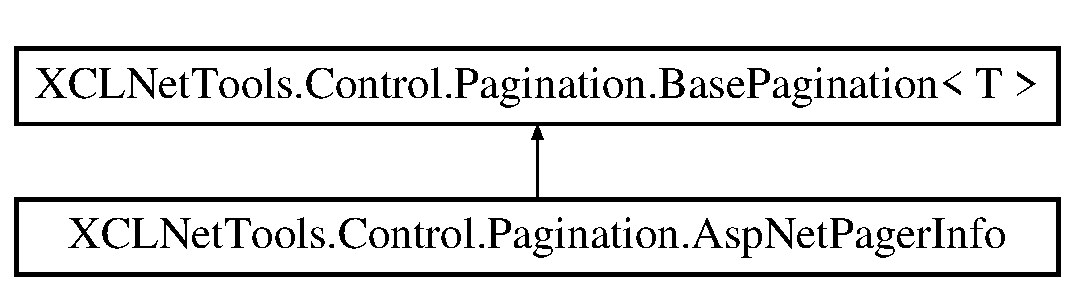
\includegraphics[height=2.000000cm]{class_x_c_l_net_tools_1_1_control_1_1_pagination_1_1_asp_net_pager_info}
\end{center}
\end{figure}
\subsection*{Public 成员函数}
\begin{DoxyCompactItemize}
\item 
\hyperlink{class_x_c_l_net_tools_1_1_control_1_1_pagination_1_1_asp_net_pager_info_aef75d024dd66cc9d75cd61d4dddcb27b}{Asp\-Net\-Pager\-Info} (Wuqi.\-Webdiyer.\-Asp\-Net\-Pager pager, int page\-Index, int page\-Size, int record\-Count)
\begin{DoxyCompactList}\small\item\em 构造函数 \end{DoxyCompactList}\item 
override void \hyperlink{class_x_c_l_net_tools_1_1_control_1_1_pagination_1_1_asp_net_pager_info_a46b208799b1d020c45571657c707ddf0}{Init\-Pager} ()
\begin{DoxyCompactList}\small\item\em 分页控件初始化 \end{DoxyCompactList}\end{DoxyCompactItemize}
\subsection*{额外继承的成员函数}


\subsection{详细描述}
Asp\-Net\-Pager分页 分页控件来源:http\-://www.webdiyer.\-com/aspnetpager/ 



在文件 Asp\-Net\-Pager\-Info.\-cs 第 15 行定义.



\subsection{构造及析构函数说明}
\hypertarget{class_x_c_l_net_tools_1_1_control_1_1_pagination_1_1_asp_net_pager_info_aef75d024dd66cc9d75cd61d4dddcb27b}{\index{X\-C\-L\-Net\-Tools\-::\-Control\-::\-Pagination\-::\-Asp\-Net\-Pager\-Info@{X\-C\-L\-Net\-Tools\-::\-Control\-::\-Pagination\-::\-Asp\-Net\-Pager\-Info}!Asp\-Net\-Pager\-Info@{Asp\-Net\-Pager\-Info}}
\index{Asp\-Net\-Pager\-Info@{Asp\-Net\-Pager\-Info}!XCLNetTools::Control::Pagination::AspNetPagerInfo@{X\-C\-L\-Net\-Tools\-::\-Control\-::\-Pagination\-::\-Asp\-Net\-Pager\-Info}}
\subsubsection[{Asp\-Net\-Pager\-Info}]{\setlength{\rightskip}{0pt plus 5cm}X\-C\-L\-Net\-Tools.\-Control.\-Pagination.\-Asp\-Net\-Pager\-Info.\-Asp\-Net\-Pager\-Info (
\begin{DoxyParamCaption}
\item[{Wuqi.\-Webdiyer.\-Asp\-Net\-Pager}]{pager, }
\item[{int}]{page\-Index, }
\item[{int}]{page\-Size, }
\item[{int}]{record\-Count}
\end{DoxyParamCaption}
)}}\label{class_x_c_l_net_tools_1_1_control_1_1_pagination_1_1_asp_net_pager_info_aef75d024dd66cc9d75cd61d4dddcb27b}


构造函数 


\begin{DoxyParams}{参数}
{\em pager} & 分页控件对象\\
\hline
{\em page\-Index} & 当前页码\\
\hline
{\em page\-Size} & 每页最多显示的记录数\\
\hline
{\em record\-Count} & 记录总数\\
\hline
\end{DoxyParams}


在文件 Asp\-Net\-Pager\-Info.\-cs 第 24 行定义.



\subsection{成员函数说明}
\hypertarget{class_x_c_l_net_tools_1_1_control_1_1_pagination_1_1_asp_net_pager_info_a46b208799b1d020c45571657c707ddf0}{\index{X\-C\-L\-Net\-Tools\-::\-Control\-::\-Pagination\-::\-Asp\-Net\-Pager\-Info@{X\-C\-L\-Net\-Tools\-::\-Control\-::\-Pagination\-::\-Asp\-Net\-Pager\-Info}!Init\-Pager@{Init\-Pager}}
\index{Init\-Pager@{Init\-Pager}!XCLNetTools::Control::Pagination::AspNetPagerInfo@{X\-C\-L\-Net\-Tools\-::\-Control\-::\-Pagination\-::\-Asp\-Net\-Pager\-Info}}
\subsubsection[{Init\-Pager}]{\setlength{\rightskip}{0pt plus 5cm}override void X\-C\-L\-Net\-Tools.\-Control.\-Pagination.\-Asp\-Net\-Pager\-Info.\-Init\-Pager (
\begin{DoxyParamCaption}
{}
\end{DoxyParamCaption}
)\hspace{0.3cm}{\ttfamily [virtual]}}}\label{class_x_c_l_net_tools_1_1_control_1_1_pagination_1_1_asp_net_pager_info_a46b208799b1d020c45571657c707ddf0}


分页控件初始化 



重载 \hyperlink{class_x_c_l_net_tools_1_1_control_1_1_pagination_1_1_base_pagination_3_01_t_01_4_ab3485196d5422f857f29f96bfbb2faa9}{X\-C\-L\-Net\-Tools.\-Control.\-Pagination.\-Base\-Pagination$<$ T $>$} .



在文件 Asp\-Net\-Pager\-Info.\-cs 第 32 行定义.



该类的文档由以下文件生成\-:\begin{DoxyCompactItemize}
\item 
D\-:/\-My\-Data/\-My\-Git/\-Git\-Hub/\-X\-C\-L\-Net\-Tools/\-X\-C\-L\-Net\-Tools/\-Control/\-Pagination/\hyperlink{_asp_net_pager_info_8cs}{Asp\-Net\-Pager\-Info.\-cs}\end{DoxyCompactItemize}

\hypertarget{class_x_c_l_net_tools_1_1_control_1_1_pagination_1_1_base_pagination}{}\section{X\+C\+L\+Net\+Tools.\+Control.\+Pagination.\+Base\+Pagination$<$ T $>$ 模板类 参考}
\label{class_x_c_l_net_tools_1_1_control_1_1_pagination_1_1_base_pagination}\index{X\+C\+L\+Net\+Tools.\+Control.\+Pagination.\+Base\+Pagination$<$ T $>$@{X\+C\+L\+Net\+Tools.\+Control.\+Pagination.\+Base\+Pagination$<$ T $>$}}


分页抽象类  


\subsection*{Public 成员函数}
\begin{DoxyCompactItemize}
\item 
\hyperlink{class_x_c_l_net_tools_1_1_control_1_1_pagination_1_1_base_pagination_ae9e336c1452804e7d4de12ea9fa3ddde}{Base\+Pagination} (T pager, int page\+Index, int page\+Size, int record\+Count)
\begin{DoxyCompactList}\small\item\em 构造函数 \end{DoxyCompactList}\item 
virtual void \hyperlink{class_x_c_l_net_tools_1_1_control_1_1_pagination_1_1_base_pagination_ab3485196d5422f857f29f96bfbb2faa9}{Init\+Pager} ()
\begin{DoxyCompactList}\small\item\em 分页初始化 \end{DoxyCompactList}\end{DoxyCompactItemize}
\subsection*{属性}
\begin{DoxyCompactItemize}
\item 
T \hyperlink{class_x_c_l_net_tools_1_1_control_1_1_pagination_1_1_base_pagination_ae0cfdba3ea23387da4b851c4d695d0a0}{Pager}\hspace{0.3cm}{\ttfamily  \mbox{[}get, set\mbox{]}}
\begin{DoxyCompactList}\small\item\em 当前分页控件 \end{DoxyCompactList}\item 
\hyperlink{class_x_c_l_net_tools_1_1_entity_1_1_pager_info}{X\+C\+L\+Net\+Tools.\+Entity.\+Pager\+Info} \hyperlink{class_x_c_l_net_tools_1_1_control_1_1_pagination_1_1_base_pagination_ae27d645cd692bb7471bc6236c59496a3}{Pager\+Info}\hspace{0.3cm}{\ttfamily  \mbox{[}get, set\mbox{]}}
\begin{DoxyCompactList}\small\item\em 分页信息 \end{DoxyCompactList}\end{DoxyCompactItemize}


\subsection{详细描述}
分页抽象类 



在文件 Base\+Pagination.\+cs 第 14 行定义.



\subsection{构造及析构函数说明}
\index{X\+C\+L\+Net\+Tools\+::\+Control\+::\+Pagination\+::\+Base\+Pagination@{X\+C\+L\+Net\+Tools\+::\+Control\+::\+Pagination\+::\+Base\+Pagination}!Base\+Pagination@{Base\+Pagination}}
\index{Base\+Pagination@{Base\+Pagination}!X\+C\+L\+Net\+Tools\+::\+Control\+::\+Pagination\+::\+Base\+Pagination@{X\+C\+L\+Net\+Tools\+::\+Control\+::\+Pagination\+::\+Base\+Pagination}}
\subsubsection[{\texorpdfstring{Base\+Pagination(\+T pager, int page\+Index, int page\+Size, int record\+Count)}{BasePagination(T pager, int pageIndex, int pageSize, int recordCount)}}]{\setlength{\rightskip}{0pt plus 5cm}{\bf X\+C\+L\+Net\+Tools.\+Control.\+Pagination.\+Base\+Pagination}$<$ T $>$.{\bf Base\+Pagination} (
\begin{DoxyParamCaption}
\item[{T}]{pager, }
\item[{int}]{page\+Index, }
\item[{int}]{page\+Size, }
\item[{int}]{record\+Count}
\end{DoxyParamCaption}
)}\hypertarget{class_x_c_l_net_tools_1_1_control_1_1_pagination_1_1_base_pagination_ae9e336c1452804e7d4de12ea9fa3ddde}{}\label{class_x_c_l_net_tools_1_1_control_1_1_pagination_1_1_base_pagination_ae9e336c1452804e7d4de12ea9fa3ddde}


构造函数 


\begin{DoxyParams}{参数}
{\em pager} & 分页控件对象\\
\hline
{\em page\+Index} & 当前页码\\
\hline
{\em page\+Size} & 每页最多显示的记录数\\
\hline
{\em record\+Count} & 记录总数\\
\hline
\end{DoxyParams}


在文件 Base\+Pagination.\+cs 第 27 行定义.



\subsection{成员函数说明}
\index{X\+C\+L\+Net\+Tools\+::\+Control\+::\+Pagination\+::\+Base\+Pagination@{X\+C\+L\+Net\+Tools\+::\+Control\+::\+Pagination\+::\+Base\+Pagination}!Init\+Pager@{Init\+Pager}}
\index{Init\+Pager@{Init\+Pager}!X\+C\+L\+Net\+Tools\+::\+Control\+::\+Pagination\+::\+Base\+Pagination@{X\+C\+L\+Net\+Tools\+::\+Control\+::\+Pagination\+::\+Base\+Pagination}}
\subsubsection[{\texorpdfstring{Init\+Pager()}{InitPager()}}]{\setlength{\rightskip}{0pt plus 5cm}virtual void {\bf X\+C\+L\+Net\+Tools.\+Control.\+Pagination.\+Base\+Pagination}$<$ T $>$.Init\+Pager (
\begin{DoxyParamCaption}
{}
\end{DoxyParamCaption}
)\hspace{0.3cm}{\ttfamily [virtual]}}\hypertarget{class_x_c_l_net_tools_1_1_control_1_1_pagination_1_1_base_pagination_ab3485196d5422f857f29f96bfbb2faa9}{}\label{class_x_c_l_net_tools_1_1_control_1_1_pagination_1_1_base_pagination_ab3485196d5422f857f29f96bfbb2faa9}


分页初始化 



被 \hyperlink{class_x_c_l_net_tools_1_1_control_1_1_pagination_1_1_asp_net_pager_info_a46b208799b1d020c45571657c707ddf0}{X\+C\+L\+Net\+Tools.\+Control.\+Pagination.\+Asp\+Net\+Pager\+Info} 重载.



在文件 Base\+Pagination.\+cs 第 47 行定义.



\subsection{属性说明}
\index{X\+C\+L\+Net\+Tools\+::\+Control\+::\+Pagination\+::\+Base\+Pagination@{X\+C\+L\+Net\+Tools\+::\+Control\+::\+Pagination\+::\+Base\+Pagination}!Pager@{Pager}}
\index{Pager@{Pager}!X\+C\+L\+Net\+Tools\+::\+Control\+::\+Pagination\+::\+Base\+Pagination@{X\+C\+L\+Net\+Tools\+::\+Control\+::\+Pagination\+::\+Base\+Pagination}}
\subsubsection[{\texorpdfstring{Pager}{Pager}}]{\setlength{\rightskip}{0pt plus 5cm}T {\bf X\+C\+L\+Net\+Tools.\+Control.\+Pagination.\+Base\+Pagination}$<$ T $>$.Pager\hspace{0.3cm}{\ttfamily [get]}, {\ttfamily [set]}}\hypertarget{class_x_c_l_net_tools_1_1_control_1_1_pagination_1_1_base_pagination_ae0cfdba3ea23387da4b851c4d695d0a0}{}\label{class_x_c_l_net_tools_1_1_control_1_1_pagination_1_1_base_pagination_ae0cfdba3ea23387da4b851c4d695d0a0}


当前分页控件 



在文件 Base\+Pagination.\+cs 第 37 行定义.

\index{X\+C\+L\+Net\+Tools\+::\+Control\+::\+Pagination\+::\+Base\+Pagination@{X\+C\+L\+Net\+Tools\+::\+Control\+::\+Pagination\+::\+Base\+Pagination}!Pager\+Info@{Pager\+Info}}
\index{Pager\+Info@{Pager\+Info}!X\+C\+L\+Net\+Tools\+::\+Control\+::\+Pagination\+::\+Base\+Pagination@{X\+C\+L\+Net\+Tools\+::\+Control\+::\+Pagination\+::\+Base\+Pagination}}
\subsubsection[{\texorpdfstring{Pager\+Info}{PagerInfo}}]{\setlength{\rightskip}{0pt plus 5cm}{\bf X\+C\+L\+Net\+Tools.\+Entity.\+Pager\+Info} {\bf X\+C\+L\+Net\+Tools.\+Control.\+Pagination.\+Base\+Pagination}$<$ T $>$.Pager\+Info\hspace{0.3cm}{\ttfamily [get]}, {\ttfamily [set]}}\hypertarget{class_x_c_l_net_tools_1_1_control_1_1_pagination_1_1_base_pagination_ae27d645cd692bb7471bc6236c59496a3}{}\label{class_x_c_l_net_tools_1_1_control_1_1_pagination_1_1_base_pagination_ae27d645cd692bb7471bc6236c59496a3}


分页信息 



在文件 Base\+Pagination.\+cs 第 42 行定义.



该类的文档由以下文件生成\+:\begin{DoxyCompactItemize}
\item 
E\+:/\+Git\+Hub/\+X\+C\+L\+Net\+Tools/\+X\+C\+L\+Net\+Tools/\+Control/\+Pagination/\hyperlink{_base_pagination_8cs}{Base\+Pagination.\+cs}\end{DoxyCompactItemize}

\hypertarget{class_x_c_l_net_tools_1_1_entity_1_1_bookmark_entity}{}\section{X\+C\+L\+Net\+Tools.\+Entity.\+Bookmark\+Entity类 参考}
\label{class_x_c_l_net_tools_1_1_entity_1_1_bookmark_entity}\index{X\+C\+L\+Net\+Tools.\+Entity.\+Bookmark\+Entity@{X\+C\+L\+Net\+Tools.\+Entity.\+Bookmark\+Entity}}


浏览器书签实体  


\subsection*{属性}
\begin{DoxyCompactItemize}
\item 
int \hyperlink{class_x_c_l_net_tools_1_1_entity_1_1_bookmark_entity_a827314c81aad0801f464f7359509baec}{Id}\hspace{0.3cm}{\ttfamily  \mbox{[}get, set\mbox{]}}
\begin{DoxyCompactList}\small\item\em 编号 \end{DoxyCompactList}\item 
int \hyperlink{class_x_c_l_net_tools_1_1_entity_1_1_bookmark_entity_afd3c2002aa8d5edeac06f6ef32ba7454}{Parent\+Id}\hspace{0.3cm}{\ttfamily  \mbox{[}get, set\mbox{]}}
\begin{DoxyCompactList}\small\item\em 父id \end{DoxyCompactList}\item 
bool \hyperlink{class_x_c_l_net_tools_1_1_entity_1_1_bookmark_entity_a025f1606c5b38103058567b3e08afe03}{Is\+Folder}\hspace{0.3cm}{\ttfamily  \mbox{[}get, set\mbox{]}}
\begin{DoxyCompactList}\small\item\em 是否为文件夹 \end{DoxyCompactList}\item 
string \hyperlink{class_x_c_l_net_tools_1_1_entity_1_1_bookmark_entity_a89ccb517e285bfdd17981a72f590bc1c}{Name}\hspace{0.3cm}{\ttfamily  \mbox{[}get, set\mbox{]}}
\begin{DoxyCompactList}\small\item\em 书签名称 \end{DoxyCompactList}\item 
string \hyperlink{class_x_c_l_net_tools_1_1_entity_1_1_bookmark_entity_af370dbfd32e8cde501e305c6999c077b}{Ico\+U\+RL}\hspace{0.3cm}{\ttfamily  \mbox{[}get, set\mbox{]}}
\begin{DoxyCompactList}\small\item\em ico图标地址 \end{DoxyCompactList}\item 
string \hyperlink{class_x_c_l_net_tools_1_1_entity_1_1_bookmark_entity_a88ebfe2441fd5804a82f5eaee1ce3232}{Url}\hspace{0.3cm}{\ttfamily  \mbox{[}get, set\mbox{]}}
\begin{DoxyCompactList}\small\item\em 书签链接 \end{DoxyCompactList}\end{DoxyCompactItemize}


\subsection{详细描述}
浏览器书签实体 



在文件 Bookmark\+Entity.\+cs 第 17 行定义.



\subsection{属性说明}
\index{X\+C\+L\+Net\+Tools\+::\+Entity\+::\+Bookmark\+Entity@{X\+C\+L\+Net\+Tools\+::\+Entity\+::\+Bookmark\+Entity}!Ico\+U\+RL@{Ico\+U\+RL}}
\index{Ico\+U\+RL@{Ico\+U\+RL}!X\+C\+L\+Net\+Tools\+::\+Entity\+::\+Bookmark\+Entity@{X\+C\+L\+Net\+Tools\+::\+Entity\+::\+Bookmark\+Entity}}
\subsubsection[{\texorpdfstring{Ico\+U\+RL}{IcoURL}}]{\setlength{\rightskip}{0pt plus 5cm}string X\+C\+L\+Net\+Tools.\+Entity.\+Bookmark\+Entity.\+Ico\+U\+RL\hspace{0.3cm}{\ttfamily [get]}, {\ttfamily [set]}}\hypertarget{class_x_c_l_net_tools_1_1_entity_1_1_bookmark_entity_af370dbfd32e8cde501e305c6999c077b}{}\label{class_x_c_l_net_tools_1_1_entity_1_1_bookmark_entity_af370dbfd32e8cde501e305c6999c077b}


ico图标地址 



在文件 Bookmark\+Entity.\+cs 第 42 行定义.

\index{X\+C\+L\+Net\+Tools\+::\+Entity\+::\+Bookmark\+Entity@{X\+C\+L\+Net\+Tools\+::\+Entity\+::\+Bookmark\+Entity}!Id@{Id}}
\index{Id@{Id}!X\+C\+L\+Net\+Tools\+::\+Entity\+::\+Bookmark\+Entity@{X\+C\+L\+Net\+Tools\+::\+Entity\+::\+Bookmark\+Entity}}
\subsubsection[{\texorpdfstring{Id}{Id}}]{\setlength{\rightskip}{0pt plus 5cm}int X\+C\+L\+Net\+Tools.\+Entity.\+Bookmark\+Entity.\+Id\hspace{0.3cm}{\ttfamily [get]}, {\ttfamily [set]}}\hypertarget{class_x_c_l_net_tools_1_1_entity_1_1_bookmark_entity_a827314c81aad0801f464f7359509baec}{}\label{class_x_c_l_net_tools_1_1_entity_1_1_bookmark_entity_a827314c81aad0801f464f7359509baec}


编号 



在文件 Bookmark\+Entity.\+cs 第 22 行定义.

\index{X\+C\+L\+Net\+Tools\+::\+Entity\+::\+Bookmark\+Entity@{X\+C\+L\+Net\+Tools\+::\+Entity\+::\+Bookmark\+Entity}!Is\+Folder@{Is\+Folder}}
\index{Is\+Folder@{Is\+Folder}!X\+C\+L\+Net\+Tools\+::\+Entity\+::\+Bookmark\+Entity@{X\+C\+L\+Net\+Tools\+::\+Entity\+::\+Bookmark\+Entity}}
\subsubsection[{\texorpdfstring{Is\+Folder}{IsFolder}}]{\setlength{\rightskip}{0pt plus 5cm}bool X\+C\+L\+Net\+Tools.\+Entity.\+Bookmark\+Entity.\+Is\+Folder\hspace{0.3cm}{\ttfamily [get]}, {\ttfamily [set]}}\hypertarget{class_x_c_l_net_tools_1_1_entity_1_1_bookmark_entity_a025f1606c5b38103058567b3e08afe03}{}\label{class_x_c_l_net_tools_1_1_entity_1_1_bookmark_entity_a025f1606c5b38103058567b3e08afe03}


是否为文件夹 



在文件 Bookmark\+Entity.\+cs 第 32 行定义.

\index{X\+C\+L\+Net\+Tools\+::\+Entity\+::\+Bookmark\+Entity@{X\+C\+L\+Net\+Tools\+::\+Entity\+::\+Bookmark\+Entity}!Name@{Name}}
\index{Name@{Name}!X\+C\+L\+Net\+Tools\+::\+Entity\+::\+Bookmark\+Entity@{X\+C\+L\+Net\+Tools\+::\+Entity\+::\+Bookmark\+Entity}}
\subsubsection[{\texorpdfstring{Name}{Name}}]{\setlength{\rightskip}{0pt plus 5cm}string X\+C\+L\+Net\+Tools.\+Entity.\+Bookmark\+Entity.\+Name\hspace{0.3cm}{\ttfamily [get]}, {\ttfamily [set]}}\hypertarget{class_x_c_l_net_tools_1_1_entity_1_1_bookmark_entity_a89ccb517e285bfdd17981a72f590bc1c}{}\label{class_x_c_l_net_tools_1_1_entity_1_1_bookmark_entity_a89ccb517e285bfdd17981a72f590bc1c}


书签名称 



在文件 Bookmark\+Entity.\+cs 第 37 行定义.

\index{X\+C\+L\+Net\+Tools\+::\+Entity\+::\+Bookmark\+Entity@{X\+C\+L\+Net\+Tools\+::\+Entity\+::\+Bookmark\+Entity}!Parent\+Id@{Parent\+Id}}
\index{Parent\+Id@{Parent\+Id}!X\+C\+L\+Net\+Tools\+::\+Entity\+::\+Bookmark\+Entity@{X\+C\+L\+Net\+Tools\+::\+Entity\+::\+Bookmark\+Entity}}
\subsubsection[{\texorpdfstring{Parent\+Id}{ParentId}}]{\setlength{\rightskip}{0pt plus 5cm}int X\+C\+L\+Net\+Tools.\+Entity.\+Bookmark\+Entity.\+Parent\+Id\hspace{0.3cm}{\ttfamily [get]}, {\ttfamily [set]}}\hypertarget{class_x_c_l_net_tools_1_1_entity_1_1_bookmark_entity_afd3c2002aa8d5edeac06f6ef32ba7454}{}\label{class_x_c_l_net_tools_1_1_entity_1_1_bookmark_entity_afd3c2002aa8d5edeac06f6ef32ba7454}


父id 



在文件 Bookmark\+Entity.\+cs 第 27 行定义.

\index{X\+C\+L\+Net\+Tools\+::\+Entity\+::\+Bookmark\+Entity@{X\+C\+L\+Net\+Tools\+::\+Entity\+::\+Bookmark\+Entity}!Url@{Url}}
\index{Url@{Url}!X\+C\+L\+Net\+Tools\+::\+Entity\+::\+Bookmark\+Entity@{X\+C\+L\+Net\+Tools\+::\+Entity\+::\+Bookmark\+Entity}}
\subsubsection[{\texorpdfstring{Url}{Url}}]{\setlength{\rightskip}{0pt plus 5cm}string X\+C\+L\+Net\+Tools.\+Entity.\+Bookmark\+Entity.\+Url\hspace{0.3cm}{\ttfamily [get]}, {\ttfamily [set]}}\hypertarget{class_x_c_l_net_tools_1_1_entity_1_1_bookmark_entity_a88ebfe2441fd5804a82f5eaee1ce3232}{}\label{class_x_c_l_net_tools_1_1_entity_1_1_bookmark_entity_a88ebfe2441fd5804a82f5eaee1ce3232}


书签链接 



在文件 Bookmark\+Entity.\+cs 第 47 行定义.



该类的文档由以下文件生成\+:\begin{DoxyCompactItemize}
\item 
E\+:/\+Git\+Hub/\+X\+C\+L\+Net\+Tools/\+X\+C\+L\+Net\+Tools/\+Entity/\hyperlink{_bookmark_entity_8cs}{Bookmark\+Entity.\+cs}\end{DoxyCompactItemize}

\hypertarget{class_x_c_l_net_tools_1_1_file_handler_1_1_download_event_args}{}\section{X\+C\+L\+Net\+Tools.\+File\+Handler.\+Download\+Event\+Args类 参考}
\label{class_x_c_l_net_tools_1_1_file_handler_1_1_download_event_args}\index{X\+C\+L\+Net\+Tools.\+File\+Handler.\+Download\+Event\+Args@{X\+C\+L\+Net\+Tools.\+File\+Handler.\+Download\+Event\+Args}}


下载数据参数  


类 X\+C\+L\+Net\+Tools.\+File\+Handler.\+Download\+Event\+Args 继承关系图\+:\begin{figure}[H]
\begin{center}
\leavevmode
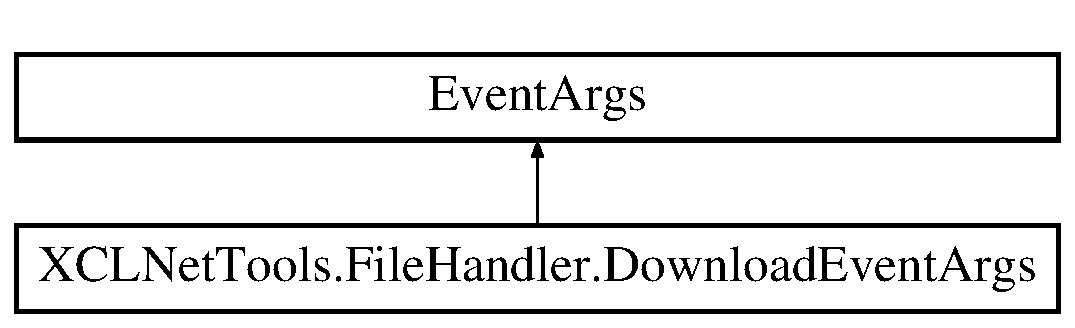
\includegraphics[height=2.000000cm]{class_x_c_l_net_tools_1_1_file_handler_1_1_download_event_args}
\end{center}
\end{figure}
\subsection*{属性}
\begin{DoxyCompactItemize}
\item 
int \hyperlink{class_x_c_l_net_tools_1_1_file_handler_1_1_download_event_args_a1ea772d1ec4b2e0f1f3001fe069bac42}{Bytes\+Received}\hspace{0.3cm}{\ttfamily  \mbox{[}get, set\mbox{]}}
\begin{DoxyCompactList}\small\item\em 已接收的字节数 \end{DoxyCompactList}\item 
int \hyperlink{class_x_c_l_net_tools_1_1_file_handler_1_1_download_event_args_a344cbcca5a213a50ecd25b90340be816}{Total\+Bytes}\hspace{0.3cm}{\ttfamily  \mbox{[}get, set\mbox{]}}
\begin{DoxyCompactList}\small\item\em 总字节数 \end{DoxyCompactList}\item 
byte\mbox{[}$\,$\mbox{]} \hyperlink{class_x_c_l_net_tools_1_1_file_handler_1_1_download_event_args_ae080073b3629650c3befb398e9d7c2e8}{Received\+Data}\hspace{0.3cm}{\ttfamily  \mbox{[}get, set\mbox{]}}
\begin{DoxyCompactList}\small\item\em 当前缓冲区接收的数据 \end{DoxyCompactList}\end{DoxyCompactItemize}


\subsection{详细描述}
下载数据参数 



在文件 Http\+Proc.\+cs 第 50 行定义.



\subsection{属性说明}
\index{X\+C\+L\+Net\+Tools\+::\+File\+Handler\+::\+Download\+Event\+Args@{X\+C\+L\+Net\+Tools\+::\+File\+Handler\+::\+Download\+Event\+Args}!Bytes\+Received@{Bytes\+Received}}
\index{Bytes\+Received@{Bytes\+Received}!X\+C\+L\+Net\+Tools\+::\+File\+Handler\+::\+Download\+Event\+Args@{X\+C\+L\+Net\+Tools\+::\+File\+Handler\+::\+Download\+Event\+Args}}
\subsubsection[{\texorpdfstring{Bytes\+Received}{BytesReceived}}]{\setlength{\rightskip}{0pt plus 5cm}int X\+C\+L\+Net\+Tools.\+File\+Handler.\+Download\+Event\+Args.\+Bytes\+Received\hspace{0.3cm}{\ttfamily [get]}, {\ttfamily [set]}}\hypertarget{class_x_c_l_net_tools_1_1_file_handler_1_1_download_event_args_a1ea772d1ec4b2e0f1f3001fe069bac42}{}\label{class_x_c_l_net_tools_1_1_file_handler_1_1_download_event_args_a1ea772d1ec4b2e0f1f3001fe069bac42}


已接收的字节数 



在文件 Http\+Proc.\+cs 第 60 行定义.

\index{X\+C\+L\+Net\+Tools\+::\+File\+Handler\+::\+Download\+Event\+Args@{X\+C\+L\+Net\+Tools\+::\+File\+Handler\+::\+Download\+Event\+Args}!Received\+Data@{Received\+Data}}
\index{Received\+Data@{Received\+Data}!X\+C\+L\+Net\+Tools\+::\+File\+Handler\+::\+Download\+Event\+Args@{X\+C\+L\+Net\+Tools\+::\+File\+Handler\+::\+Download\+Event\+Args}}
\subsubsection[{\texorpdfstring{Received\+Data}{ReceivedData}}]{\setlength{\rightskip}{0pt plus 5cm}byte \mbox{[}$\,$\mbox{]} X\+C\+L\+Net\+Tools.\+File\+Handler.\+Download\+Event\+Args.\+Received\+Data\hspace{0.3cm}{\ttfamily [get]}, {\ttfamily [set]}}\hypertarget{class_x_c_l_net_tools_1_1_file_handler_1_1_download_event_args_ae080073b3629650c3befb398e9d7c2e8}{}\label{class_x_c_l_net_tools_1_1_file_handler_1_1_download_event_args_ae080073b3629650c3befb398e9d7c2e8}


当前缓冲区接收的数据 



在文件 Http\+Proc.\+cs 第 78 行定义.

\index{X\+C\+L\+Net\+Tools\+::\+File\+Handler\+::\+Download\+Event\+Args@{X\+C\+L\+Net\+Tools\+::\+File\+Handler\+::\+Download\+Event\+Args}!Total\+Bytes@{Total\+Bytes}}
\index{Total\+Bytes@{Total\+Bytes}!X\+C\+L\+Net\+Tools\+::\+File\+Handler\+::\+Download\+Event\+Args@{X\+C\+L\+Net\+Tools\+::\+File\+Handler\+::\+Download\+Event\+Args}}
\subsubsection[{\texorpdfstring{Total\+Bytes}{TotalBytes}}]{\setlength{\rightskip}{0pt plus 5cm}int X\+C\+L\+Net\+Tools.\+File\+Handler.\+Download\+Event\+Args.\+Total\+Bytes\hspace{0.3cm}{\ttfamily [get]}, {\ttfamily [set]}}\hypertarget{class_x_c_l_net_tools_1_1_file_handler_1_1_download_event_args_a344cbcca5a213a50ecd25b90340be816}{}\label{class_x_c_l_net_tools_1_1_file_handler_1_1_download_event_args_a344cbcca5a213a50ecd25b90340be816}


总字节数 



在文件 Http\+Proc.\+cs 第 69 行定义.



该类的文档由以下文件生成\+:\begin{DoxyCompactItemize}
\item 
E\+:/\+Git\+Hub/\+X\+C\+L\+Net\+Tools/\+X\+C\+L\+Net\+Tools/\+File\+Handler/\hyperlink{_http_proc_8cs}{Http\+Proc.\+cs}\end{DoxyCompactItemize}

\hypertarget{class_x_c_l_net_tools_1_1_entity_1_1_enum_1_1_enum_field_model}{\section{X\-C\-L\-Net\-Tools.\-Entity.\-Enum.\-Enum\-Field\-Model类 参考}
\label{class_x_c_l_net_tools_1_1_entity_1_1_enum_1_1_enum_field_model}\index{X\-C\-L\-Net\-Tools.\-Entity.\-Enum.\-Enum\-Field\-Model@{X\-C\-L\-Net\-Tools.\-Entity.\-Enum.\-Enum\-Field\-Model}}
}


Enum项model  


\subsection*{属性}
\begin{DoxyCompactItemize}
\item 
string \hyperlink{class_x_c_l_net_tools_1_1_entity_1_1_enum_1_1_enum_field_model_afba0a6a9289087c382b5d8050ff4dcd0}{Text}\hspace{0.3cm}{\ttfamily  \mbox{[}get, set\mbox{]}}
\begin{DoxyCompactList}\small\item\em text值 \end{DoxyCompactList}\item 
string \hyperlink{class_x_c_l_net_tools_1_1_entity_1_1_enum_1_1_enum_field_model_aa2c519a0507eff410068ee108e7ed845}{Value}\hspace{0.3cm}{\ttfamily  \mbox{[}get, set\mbox{]}}
\begin{DoxyCompactList}\small\item\em value值 \end{DoxyCompactList}\item 
string \hyperlink{class_x_c_l_net_tools_1_1_entity_1_1_enum_1_1_enum_field_model_aac9ea6b895da17a78a261f2721a6da08}{Description}\hspace{0.3cm}{\ttfamily  \mbox{[}get, set\mbox{]}}
\begin{DoxyCompactList}\small\item\em description特性 \end{DoxyCompactList}\end{DoxyCompactItemize}


\subsection{详细描述}
Enum项model 



在文件 Enum\-Field\-Model.\-cs 第 33 行定义.



\subsection{属性说明}
\hypertarget{class_x_c_l_net_tools_1_1_entity_1_1_enum_1_1_enum_field_model_aac9ea6b895da17a78a261f2721a6da08}{\index{X\-C\-L\-Net\-Tools\-::\-Entity\-::\-Enum\-::\-Enum\-Field\-Model@{X\-C\-L\-Net\-Tools\-::\-Entity\-::\-Enum\-::\-Enum\-Field\-Model}!Description@{Description}}
\index{Description@{Description}!XCLNetTools::Entity::Enum::EnumFieldModel@{X\-C\-L\-Net\-Tools\-::\-Entity\-::\-Enum\-::\-Enum\-Field\-Model}}
\subsubsection[{Description}]{\setlength{\rightskip}{0pt plus 5cm}string X\-C\-L\-Net\-Tools.\-Entity.\-Enum.\-Enum\-Field\-Model.\-Description\hspace{0.3cm}{\ttfamily [get]}, {\ttfamily [set]}}}\label{class_x_c_l_net_tools_1_1_entity_1_1_enum_1_1_enum_field_model_aac9ea6b895da17a78a261f2721a6da08}


description特性 



在文件 Enum\-Field\-Model.\-cs 第 48 行定义.

\hypertarget{class_x_c_l_net_tools_1_1_entity_1_1_enum_1_1_enum_field_model_afba0a6a9289087c382b5d8050ff4dcd0}{\index{X\-C\-L\-Net\-Tools\-::\-Entity\-::\-Enum\-::\-Enum\-Field\-Model@{X\-C\-L\-Net\-Tools\-::\-Entity\-::\-Enum\-::\-Enum\-Field\-Model}!Text@{Text}}
\index{Text@{Text}!XCLNetTools::Entity::Enum::EnumFieldModel@{X\-C\-L\-Net\-Tools\-::\-Entity\-::\-Enum\-::\-Enum\-Field\-Model}}
\subsubsection[{Text}]{\setlength{\rightskip}{0pt plus 5cm}string X\-C\-L\-Net\-Tools.\-Entity.\-Enum.\-Enum\-Field\-Model.\-Text\hspace{0.3cm}{\ttfamily [get]}, {\ttfamily [set]}}}\label{class_x_c_l_net_tools_1_1_entity_1_1_enum_1_1_enum_field_model_afba0a6a9289087c382b5d8050ff4dcd0}


text值 



在文件 Enum\-Field\-Model.\-cs 第 38 行定义.

\hypertarget{class_x_c_l_net_tools_1_1_entity_1_1_enum_1_1_enum_field_model_aa2c519a0507eff410068ee108e7ed845}{\index{X\-C\-L\-Net\-Tools\-::\-Entity\-::\-Enum\-::\-Enum\-Field\-Model@{X\-C\-L\-Net\-Tools\-::\-Entity\-::\-Enum\-::\-Enum\-Field\-Model}!Value@{Value}}
\index{Value@{Value}!XCLNetTools::Entity::Enum::EnumFieldModel@{X\-C\-L\-Net\-Tools\-::\-Entity\-::\-Enum\-::\-Enum\-Field\-Model}}
\subsubsection[{Value}]{\setlength{\rightskip}{0pt plus 5cm}string X\-C\-L\-Net\-Tools.\-Entity.\-Enum.\-Enum\-Field\-Model.\-Value\hspace{0.3cm}{\ttfamily [get]}, {\ttfamily [set]}}}\label{class_x_c_l_net_tools_1_1_entity_1_1_enum_1_1_enum_field_model_aa2c519a0507eff410068ee108e7ed845}


value值 



在文件 Enum\-Field\-Model.\-cs 第 43 行定义.



该类的文档由以下文件生成\-:\begin{DoxyCompactItemize}
\item 
D\-:/\-My\-Data/\-My\-Git/\-Git\-Hub/\-X\-C\-L\-Net\-Tools/\-X\-C\-L\-Net\-Tools/\-Entity/\-Enum/\hyperlink{_enum_field_model_8cs}{Enum\-Field\-Model.\-cs}\end{DoxyCompactItemize}

\hypertarget{class_x_c_l_net_tools_1_1_entity_1_1_enum_1_1_enum_field_t_model}{}\section{X\+C\+L\+Net\+Tools.\+Entity.\+Enum.\+Enum\+Field\+T\+Model$<$ T $>$ 模板类 参考}
\label{class_x_c_l_net_tools_1_1_entity_1_1_enum_1_1_enum_field_t_model}\index{X\+C\+L\+Net\+Tools.\+Entity.\+Enum.\+Enum\+Field\+T\+Model$<$ T $>$@{X\+C\+L\+Net\+Tools.\+Entity.\+Enum.\+Enum\+Field\+T\+Model$<$ T $>$}}


枚举model  


\subsection*{属性}
\begin{DoxyCompactItemize}
\item 
string \hyperlink{class_x_c_l_net_tools_1_1_entity_1_1_enum_1_1_enum_field_t_model_a19570f5fcd9bb314ca1e7e8f3b8f44b1}{Text}\hspace{0.3cm}{\ttfamily  \mbox{[}get, set\mbox{]}}
\begin{DoxyCompactList}\small\item\em text值 \end{DoxyCompactList}\item 
T \hyperlink{class_x_c_l_net_tools_1_1_entity_1_1_enum_1_1_enum_field_t_model_a0b6e9efa5eb3b809fdc2bbb675a4e8e3}{Value}\hspace{0.3cm}{\ttfamily  \mbox{[}get, set\mbox{]}}
\begin{DoxyCompactList}\small\item\em value值 \end{DoxyCompactList}\item 
string \hyperlink{class_x_c_l_net_tools_1_1_entity_1_1_enum_1_1_enum_field_t_model_a6702736fc7d4f0f7cfefb74722f9c2ba}{Description}\hspace{0.3cm}{\ttfamily  \mbox{[}get, set\mbox{]}}
\begin{DoxyCompactList}\small\item\em description特性 \end{DoxyCompactList}\end{DoxyCompactItemize}


\subsection{详细描述}
枚举model 


\begin{DoxyTemplParams}{Template Parameters}
{\em T} & 枚举value值类型(可为byte、sbyte、short、ushort、int、uint、long 或 ulong。)\\
\hline
\end{DoxyTemplParams}


在文件 Enum\+Field\+T\+Model.\+cs 第 18 行定义.



\subsection{属性说明}
\mbox{\Hypertarget{class_x_c_l_net_tools_1_1_entity_1_1_enum_1_1_enum_field_t_model_a6702736fc7d4f0f7cfefb74722f9c2ba}\label{class_x_c_l_net_tools_1_1_entity_1_1_enum_1_1_enum_field_t_model_a6702736fc7d4f0f7cfefb74722f9c2ba}} 
\index{X\+C\+L\+Net\+Tools\+::\+Entity\+::\+Enum\+::\+Enum\+Field\+T\+Model@{X\+C\+L\+Net\+Tools\+::\+Entity\+::\+Enum\+::\+Enum\+Field\+T\+Model}!Description@{Description}}
\index{Description@{Description}!X\+C\+L\+Net\+Tools\+::\+Entity\+::\+Enum\+::\+Enum\+Field\+T\+Model@{X\+C\+L\+Net\+Tools\+::\+Entity\+::\+Enum\+::\+Enum\+Field\+T\+Model}}
\subsubsection{\texorpdfstring{Description}{Description}}
{\footnotesize\ttfamily string \hyperlink{class_x_c_l_net_tools_1_1_entity_1_1_enum_1_1_enum_field_t_model}{X\+C\+L\+Net\+Tools.\+Entity.\+Enum.\+Enum\+Field\+T\+Model}$<$ T $>$.Description\hspace{0.3cm}{\ttfamily [get]}, {\ttfamily [set]}}



description特性 



在文件 Enum\+Field\+T\+Model.\+cs 第 33 行定义.

\mbox{\Hypertarget{class_x_c_l_net_tools_1_1_entity_1_1_enum_1_1_enum_field_t_model_a19570f5fcd9bb314ca1e7e8f3b8f44b1}\label{class_x_c_l_net_tools_1_1_entity_1_1_enum_1_1_enum_field_t_model_a19570f5fcd9bb314ca1e7e8f3b8f44b1}} 
\index{X\+C\+L\+Net\+Tools\+::\+Entity\+::\+Enum\+::\+Enum\+Field\+T\+Model@{X\+C\+L\+Net\+Tools\+::\+Entity\+::\+Enum\+::\+Enum\+Field\+T\+Model}!Text@{Text}}
\index{Text@{Text}!X\+C\+L\+Net\+Tools\+::\+Entity\+::\+Enum\+::\+Enum\+Field\+T\+Model@{X\+C\+L\+Net\+Tools\+::\+Entity\+::\+Enum\+::\+Enum\+Field\+T\+Model}}
\subsubsection{\texorpdfstring{Text}{Text}}
{\footnotesize\ttfamily string \hyperlink{class_x_c_l_net_tools_1_1_entity_1_1_enum_1_1_enum_field_t_model}{X\+C\+L\+Net\+Tools.\+Entity.\+Enum.\+Enum\+Field\+T\+Model}$<$ T $>$.Text\hspace{0.3cm}{\ttfamily [get]}, {\ttfamily [set]}}



text值 



在文件 Enum\+Field\+T\+Model.\+cs 第 23 行定义.

\mbox{\Hypertarget{class_x_c_l_net_tools_1_1_entity_1_1_enum_1_1_enum_field_t_model_a0b6e9efa5eb3b809fdc2bbb675a4e8e3}\label{class_x_c_l_net_tools_1_1_entity_1_1_enum_1_1_enum_field_t_model_a0b6e9efa5eb3b809fdc2bbb675a4e8e3}} 
\index{X\+C\+L\+Net\+Tools\+::\+Entity\+::\+Enum\+::\+Enum\+Field\+T\+Model@{X\+C\+L\+Net\+Tools\+::\+Entity\+::\+Enum\+::\+Enum\+Field\+T\+Model}!Value@{Value}}
\index{Value@{Value}!X\+C\+L\+Net\+Tools\+::\+Entity\+::\+Enum\+::\+Enum\+Field\+T\+Model@{X\+C\+L\+Net\+Tools\+::\+Entity\+::\+Enum\+::\+Enum\+Field\+T\+Model}}
\subsubsection{\texorpdfstring{Value}{Value}}
{\footnotesize\ttfamily T \hyperlink{class_x_c_l_net_tools_1_1_entity_1_1_enum_1_1_enum_field_t_model}{X\+C\+L\+Net\+Tools.\+Entity.\+Enum.\+Enum\+Field\+T\+Model}$<$ T $>$.Value\hspace{0.3cm}{\ttfamily [get]}, {\ttfamily [set]}}



value值 



在文件 Enum\+Field\+T\+Model.\+cs 第 28 行定义.



该类的文档由以下文件生成\+:\begin{DoxyCompactItemize}
\item 
D\+:/\+My\+Data/\+Git\+Hub/\+X\+C\+L\+Net\+Tools/\+X\+C\+L\+Net\+Tools/\+Entity/\+Enum/\hyperlink{_enum_field_t_model_8cs}{Enum\+Field\+T\+Model.\+cs}\end{DoxyCompactItemize}

\hypertarget{class_x_c_l_net_tools_1_1_modules_1_1_error_http_module}{}\section{X\+C\+L\+Net\+Tools.\+Modules.\+Error\+Http\+Module类 参考}
\label{class_x_c_l_net_tools_1_1_modules_1_1_error_http_module}\index{X\+C\+L\+Net\+Tools.\+Modules.\+Error\+Http\+Module@{X\+C\+L\+Net\+Tools.\+Modules.\+Error\+Http\+Module}}


异常处理  


类 X\+C\+L\+Net\+Tools.\+Modules.\+Error\+Http\+Module 继承关系图\+:\begin{figure}[H]
\begin{center}
\leavevmode
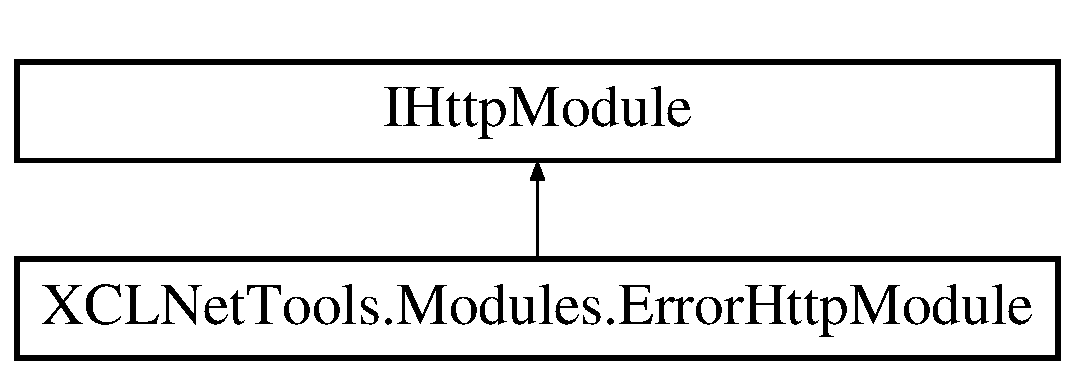
\includegraphics[height=2.000000cm]{class_x_c_l_net_tools_1_1_modules_1_1_error_http_module}
\end{center}
\end{figure}
\subsection*{Public 成员函数}
\begin{DoxyCompactItemize}
\item 
void \hyperlink{class_x_c_l_net_tools_1_1_modules_1_1_error_http_module_a54025f294511e299dd7d5b5c2f33e8ce}{Init} (Http\+Application context)
\begin{DoxyCompactList}\small\item\em 初始化 \end{DoxyCompactList}\item 
void \hyperlink{class_x_c_l_net_tools_1_1_modules_1_1_error_http_module_a86a6bafb14f79ec0551a632f07e90e6d}{Dispose} ()
\begin{DoxyCompactList}\small\item\em Dispose \end{DoxyCompactList}\end{DoxyCompactItemize}


\subsection{详细描述}
异常处理 



在文件 Error\+Http\+Module.\+cs 第 19 行定义.



\subsection{成员函数说明}
\mbox{\Hypertarget{class_x_c_l_net_tools_1_1_modules_1_1_error_http_module_a86a6bafb14f79ec0551a632f07e90e6d}\label{class_x_c_l_net_tools_1_1_modules_1_1_error_http_module_a86a6bafb14f79ec0551a632f07e90e6d}} 
\index{X\+C\+L\+Net\+Tools\+::\+Modules\+::\+Error\+Http\+Module@{X\+C\+L\+Net\+Tools\+::\+Modules\+::\+Error\+Http\+Module}!Dispose@{Dispose}}
\index{Dispose@{Dispose}!X\+C\+L\+Net\+Tools\+::\+Modules\+::\+Error\+Http\+Module@{X\+C\+L\+Net\+Tools\+::\+Modules\+::\+Error\+Http\+Module}}
\subsubsection{\texorpdfstring{Dispose()}{Dispose()}}
{\footnotesize\ttfamily void X\+C\+L\+Net\+Tools.\+Modules.\+Error\+Http\+Module.\+Dispose (\begin{DoxyParamCaption}{ }\end{DoxyParamCaption})}



Dispose 



在文件 Error\+Http\+Module.\+cs 第 78 行定义.

\mbox{\Hypertarget{class_x_c_l_net_tools_1_1_modules_1_1_error_http_module_a54025f294511e299dd7d5b5c2f33e8ce}\label{class_x_c_l_net_tools_1_1_modules_1_1_error_http_module_a54025f294511e299dd7d5b5c2f33e8ce}} 
\index{X\+C\+L\+Net\+Tools\+::\+Modules\+::\+Error\+Http\+Module@{X\+C\+L\+Net\+Tools\+::\+Modules\+::\+Error\+Http\+Module}!Init@{Init}}
\index{Init@{Init}!X\+C\+L\+Net\+Tools\+::\+Modules\+::\+Error\+Http\+Module@{X\+C\+L\+Net\+Tools\+::\+Modules\+::\+Error\+Http\+Module}}
\subsubsection{\texorpdfstring{Init()}{Init()}}
{\footnotesize\ttfamily void X\+C\+L\+Net\+Tools.\+Modules.\+Error\+Http\+Module.\+Init (\begin{DoxyParamCaption}\item[{Http\+Application}]{context }\end{DoxyParamCaption})}



初始化 



在文件 Error\+Http\+Module.\+cs 第 26 行定义.



该类的文档由以下文件生成\+:\begin{DoxyCompactItemize}
\item 
D\+:/\+My\+Data/\+Git\+Hub/\+X\+C\+L\+Net\+Tools/\+X\+C\+L\+Net\+Tools/\+Modules/\hyperlink{_error_http_module_8cs}{Error\+Http\+Module.\+cs}\end{DoxyCompactItemize}

\hypertarget{class_x_c_l_net_tools_1_1_office_1_1_excel_handler_1_1_excel_helper}{}\section{X\+C\+L\+Net\+Tools.\+Office.\+Excel\+Handler.\+Excel\+Helper类 参考}
\label{class_x_c_l_net_tools_1_1_office_1_1_excel_handler_1_1_excel_helper}\index{X\+C\+L\+Net\+Tools.\+Office.\+Excel\+Handler.\+Excel\+Helper@{X\+C\+L\+Net\+Tools.\+Office.\+Excel\+Handler.\+Excel\+Helper}}


旧版的excel操作(基于excel.\+dll),建议不要使用此类(用aspose.\+cells)  


\subsection*{Public 成员函数}
\begin{DoxyCompactItemize}
\item 
\hyperlink{class_x_c_l_net_tools_1_1_office_1_1_excel_handler_1_1_excel_helper_a12c422938f2054941e10baa671676383}{Excel\+Helper} (string templet\+File\+Path, string output\+File\+Path)
\begin{DoxyCompactList}\small\item\em 构造函数,将一个已有\+Excel工作簿作为模板,并指定输出路径 \end{DoxyCompactList}\item 
\hyperlink{class_x_c_l_net_tools_1_1_office_1_1_excel_handler_1_1_excel_helper_a92dad5cbd48287b013aa81ca90d02fb6}{Excel\+Helper} (string file\+Name)
\begin{DoxyCompactList}\small\item\em 构造函数,打开一个已有的工作簿 \end{DoxyCompactList}\item 
\hyperlink{class_x_c_l_net_tools_1_1_office_1_1_excel_handler_1_1_excel_helper_ab7738aab96d5a2ebc7d5c8a72899edf1}{Excel\+Helper} ()
\begin{DoxyCompactList}\small\item\em 构造函数,新建一个工作簿 \end{DoxyCompactList}\item 
void \hyperlink{class_x_c_l_net_tools_1_1_office_1_1_excel_handler_1_1_excel_helper_aff2b9ad2316d2acf6908da2929b5a103}{Data\+Table\+To\+Excel} (Data\+Table dt, int rows, int top, int left)
\begin{DoxyCompactList}\small\item\em 将\+Data\+Table数据写入\+Excel文件(自动分页) \end{DoxyCompactList}\item 
void \hyperlink{class_x_c_l_net_tools_1_1_office_1_1_excel_handler_1_1_excel_helper_ad8dc84e458463633d1027acdfadc5d2c}{Data\+Table\+To\+Excel} (Data\+Table dt, int top, int left)
\begin{DoxyCompactList}\small\item\em 将\+Data\+Table数据写入\+Excel文件(不分页) \end{DoxyCompactList}\item 
void \hyperlink{class_x_c_l_net_tools_1_1_office_1_1_excel_handler_1_1_excel_helper_a0d9c977adcc92c1e57560f1d713f74be}{Data\+Table\+To\+Excel} (Data\+Table dt, int rows, int top, int left, int merge\+Column\+Index)
\begin{DoxyCompactList}\small\item\em 将\+Data\+Table数据写入\+Excel文件(自动分页,并指定要合并的列索引) \end{DoxyCompactList}\item 
void \hyperlink{class_x_c_l_net_tools_1_1_office_1_1_excel_handler_1_1_excel_helper_a030afbe0c22736247a4d56571d511d35}{Array\+To\+Excel} (string\mbox{[},\mbox{]} arr, int rows, int top, int left)
\begin{DoxyCompactList}\small\item\em 将二维数组数据写入\+Excel文件(自动分页) \end{DoxyCompactList}\item 
void \hyperlink{class_x_c_l_net_tools_1_1_office_1_1_excel_handler_1_1_excel_helper_a14572a6f3b54ae9c79abf8bceafdb899}{Array\+To\+Excel} (string\mbox{[},\mbox{]} arr, int top, int left)
\begin{DoxyCompactList}\small\item\em 将二维数组数据写入\+Excel文件(不分页) \end{DoxyCompactList}\item 
void \hyperlink{class_x_c_l_net_tools_1_1_office_1_1_excel_handler_1_1_excel_helper_af7ddc4bd7a68d157487f83a4b4525e96}{Array\+To\+Excel} (string\mbox{[},\mbox{]} arr, int top, int left, bool is\+Formula)
\begin{DoxyCompactList}\small\item\em 将二维数组数据写入\+Excel文件(不分页) \end{DoxyCompactList}\item 
void \hyperlink{class_x_c_l_net_tools_1_1_office_1_1_excel_handler_1_1_excel_helper_ae1ee324469dc2bc11d537cad8a18edab}{Array\+To\+Excel} (string\mbox{[},\mbox{]} arr, int top, int left, bool is\+Formula, int merge\+Column\+Index)
\begin{DoxyCompactList}\small\item\em 将二维数组数据写入\+Excel文件(不分页),合并指定列的相同行 \end{DoxyCompactList}\item 
void \hyperlink{class_x_c_l_net_tools_1_1_office_1_1_excel_handler_1_1_excel_helper_aad9f026e5f7ec6d4307f5755a44030f8}{Array\+To\+Excel} (int sheet\+Index, string\mbox{[},\mbox{]} arr, int top, int left)
\begin{DoxyCompactList}\small\item\em 将二维数组数据写入\+Excel文件(不分页) \end{DoxyCompactList}\item 
void \hyperlink{class_x_c_l_net_tools_1_1_office_1_1_excel_handler_1_1_excel_helper_a6d9aebcdcfc00873fa4ee3cff1b7db5f}{Array\+To\+Excel} (string\mbox{[},\mbox{]} arr, int rows, int top, int left, int merge\+Column\+Index)
\begin{DoxyCompactList}\small\item\em 将二维数组数据写入\+Excel文件(自动分页,并指定要合并的列索引) \end{DoxyCompactList}\item 
void \hyperlink{class_x_c_l_net_tools_1_1_office_1_1_excel_handler_1_1_excel_helper_a626d1643db6d20fb63ba1166043dbc31}{Change\+Current\+Work\+Sheet} (int sheet\+Index)
\begin{DoxyCompactList}\small\item\em 改变当前工作表 \end{DoxyCompactList}\item 
void \hyperlink{class_x_c_l_net_tools_1_1_office_1_1_excel_handler_1_1_excel_helper_a9aaab80ccb46c62132165fd20790e3d0}{Hidden\+Work\+Sheet} (string sheet\+Name)
\begin{DoxyCompactList}\small\item\em 隐藏指定名称的工作表 \end{DoxyCompactList}\item 
void \hyperlink{class_x_c_l_net_tools_1_1_office_1_1_excel_handler_1_1_excel_helper_a96b25f831723c0a7b3522447af7c4336}{Hidden\+Work\+Sheet} (int sheet\+Index)
\begin{DoxyCompactList}\small\item\em 隐藏指定索引的工作表 \end{DoxyCompactList}\item 
void \hyperlink{class_x_c_l_net_tools_1_1_office_1_1_excel_handler_1_1_excel_helper_a628ecdd26ecf5c685ad7c2ab076cf36b}{Copy\+Work\+Sheets} (string sheet\+Name, int sheet\+Count)
\begin{DoxyCompactList}\small\item\em 在指定名称的工作表后面拷贝指定个数的该工作表的副本,并重命名 \end{DoxyCompactList}\item 
void \hyperlink{class_x_c_l_net_tools_1_1_office_1_1_excel_handler_1_1_excel_helper_a730eefd07f0b338d62000d58b6791ca1}{Copy\+Work\+Sheet} (int src\+Sheet\+Index, int aim\+Sheet\+Index, string new\+Sheet\+Name)
\begin{DoxyCompactList}\small\item\em 将一个工作表拷贝到另一个工作表后面,并重命名 \end{DoxyCompactList}\item 
void \hyperlink{class_x_c_l_net_tools_1_1_office_1_1_excel_handler_1_1_excel_helper_adc2bee7e717436f8bc586c5a0d149d3e}{Delete\+Work\+Sheet} (string sheet\+Name)
\begin{DoxyCompactList}\small\item\em 根据名称删除工作表 \end{DoxyCompactList}\item 
void \hyperlink{class_x_c_l_net_tools_1_1_office_1_1_excel_handler_1_1_excel_helper_abbd230c249186909fa47978177315cc5}{Delete\+Work\+Sheet} (int sheet\+Index)
\begin{DoxyCompactList}\small\item\em 根据索引删除工作表 \end{DoxyCompactList}\item 
void \hyperlink{class_x_c_l_net_tools_1_1_office_1_1_excel_handler_1_1_excel_helper_a5ae2a9cc10bd517ae122b9f74608d28f}{Set\+Text\+Box} (string textbox\+Name, string text)
\begin{DoxyCompactList}\small\item\em 向指定文本框写入数据,对每个\+Work\+Sheet操作 \end{DoxyCompactList}\item 
void \hyperlink{class_x_c_l_net_tools_1_1_office_1_1_excel_handler_1_1_excel_helper_ae6999962417a5ac284af99ef3305c14e}{Set\+Text\+Box} (int sheet\+Index, string textbox\+Name, string text)
\begin{DoxyCompactList}\small\item\em 向指定文本框写入数据,对指定\+Work\+Sheet操作 \end{DoxyCompactList}\item 
void \hyperlink{class_x_c_l_net_tools_1_1_office_1_1_excel_handler_1_1_excel_helper_abb6a218200a17f2be52b999e5d458df5}{Set\+Text\+Boxes} (Hashtable ht)
\begin{DoxyCompactList}\small\item\em 向文本框写入数据,对每个\+Work\+Sheet操作 \end{DoxyCompactList}\item 
void \hyperlink{class_x_c_l_net_tools_1_1_office_1_1_excel_handler_1_1_excel_helper_afcac92ace2a349e193920ad28101dd0e}{Set\+Text\+Boxes} (int sheet\+Index, Hashtable ht)
\begin{DoxyCompactList}\small\item\em 向文本框写入数据,对指定\+Work\+Sheet操作 \end{DoxyCompactList}\item 
void \hyperlink{class_x_c_l_net_tools_1_1_office_1_1_excel_handler_1_1_excel_helper_ad69661f169802e75d2ff920d5935f99e}{Set\+Cells} (int row\+Index, int column\+Index, string text)
\begin{DoxyCompactList}\small\item\em 向单元格写入数据,对当前\+Work\+Sheet操作 \end{DoxyCompactList}\item 
void \hyperlink{class_x_c_l_net_tools_1_1_office_1_1_excel_handler_1_1_excel_helper_a8344816c7157ec0b4a2d4c7ca9e3bd4c}{Set\+Cells} (int sheet\+Index, int row\+Index, int column\+Index, string text)
\begin{DoxyCompactList}\small\item\em 向单元格写入数据,对指定\+Work\+Sheet操作 \end{DoxyCompactList}\item 
void \hyperlink{class_x_c_l_net_tools_1_1_office_1_1_excel_handler_1_1_excel_helper_acd5e584cc8280620cd132f2e92a2c464}{Set\+Cells} (Hashtable ht)
\begin{DoxyCompactList}\small\item\em 向单元格写入数据,对每个\+Work\+Sheet操作 \end{DoxyCompactList}\item 
void \hyperlink{class_x_c_l_net_tools_1_1_office_1_1_excel_handler_1_1_excel_helper_a3f5cd938e43939ab228512488ee5c843}{Set\+Cells} (int sheet\+Index, Hashtable ht)
\begin{DoxyCompactList}\small\item\em 向单元格写入数据,对指定\+Work\+Sheet操作 \end{DoxyCompactList}\item 
void \hyperlink{class_x_c_l_net_tools_1_1_office_1_1_excel_handler_1_1_excel_helper_adc471403ad84fed9a9cadbc25eda8ecf}{Set\+Cells} (int sheet\+Index, string\mbox{[}$\,$\mbox{]} arr)
\begin{DoxyCompactList}\small\item\em 设置单元格为可计算的 \end{DoxyCompactList}\item 
void \hyperlink{class_x_c_l_net_tools_1_1_office_1_1_excel_handler_1_1_excel_helper_a252fb1aa0a592429ffa639943ef6752f}{Set\+Cells} (string sheet\+Name, Hashtable ht)
\begin{DoxyCompactList}\small\item\em 向单元格写入数据,对指定\+Work\+Sheet操作 \end{DoxyCompactList}\item 
void \hyperlink{class_x_c_l_net_tools_1_1_office_1_1_excel_handler_1_1_excel_helper_a7602a33dbb3ee6cfbbf4a66e6106bd78}{Merge\+Cells} (int begin\+Row\+Index, int begin\+Column\+Index, int end\+Row\+Index, int end\+Column\+Index, string text)
\begin{DoxyCompactList}\small\item\em 合并单元格,并赋值,对每个\+Work\+Sheet操作 \end{DoxyCompactList}\item 
void \hyperlink{class_x_c_l_net_tools_1_1_office_1_1_excel_handler_1_1_excel_helper_a6285e410acdeec87d53f8720b1366d2a}{Merge\+Cells} (int sheet\+Index, int begin\+Row\+Index, int begin\+Column\+Index, int end\+Row\+Index, int end\+Column\+Index, string text)
\begin{DoxyCompactList}\small\item\em 合并单元格,并赋值,对指定\+Work\+Sheet操作 \end{DoxyCompactList}\item 
void \hyperlink{class_x_c_l_net_tools_1_1_office_1_1_excel_handler_1_1_excel_helper_a6e130b3596ed54ce811fa500ff4df20b}{Merge\+Rows} (int column\+Index, int begin\+Row\+Index, int end\+Row\+Index)
\begin{DoxyCompactList}\small\item\em 将指定索引列的数据相同的行合并,对每个\+Work\+Sheet操作 \end{DoxyCompactList}\item 
void \hyperlink{class_x_c_l_net_tools_1_1_office_1_1_excel_handler_1_1_excel_helper_acbca99c07c2d2b210e1709660d383b97}{Merge\+Rows} (int sheet\+Index, int column\+Index, int begin\+Row\+Index, int end\+Row\+Index)
\begin{DoxyCompactList}\small\item\em 将指定索引列的数据相同的行合并,对指定\+Work\+Sheet操作 \end{DoxyCompactList}\item 
void \hyperlink{class_x_c_l_net_tools_1_1_office_1_1_excel_handler_1_1_excel_helper_a2d4906537fdb886329ba5dbdfe82ed18}{Insert\+Rows} (int row\+Index, int count)
\begin{DoxyCompactList}\small\item\em 插行(在指定行上面插入指定数量行) \end{DoxyCompactList}\item 
void \hyperlink{class_x_c_l_net_tools_1_1_office_1_1_excel_handler_1_1_excel_helper_ae52b03c158a2db80aa61b3db05e9298c}{Insert\+Rows} (int sheet\+Index, int row\+Index, int count)
\begin{DoxyCompactList}\small\item\em 插行(在指定\+Work\+Sheet指定行上面插入指定数量行) \end{DoxyCompactList}\item 
void \hyperlink{class_x_c_l_net_tools_1_1_office_1_1_excel_handler_1_1_excel_helper_a7e024058407b8033da3728d18a100dc1}{Copy\+Rows} (int row\+Index, int count)
\begin{DoxyCompactList}\small\item\em 复制行(在指定行下面复制指定数量行) \end{DoxyCompactList}\item 
void \hyperlink{class_x_c_l_net_tools_1_1_office_1_1_excel_handler_1_1_excel_helper_ae5ca11d360518bfcf0ec30506120adfb}{Copy\+Rows} (int sheet\+Index, int row\+Index, int count)
\begin{DoxyCompactList}\small\item\em 复制行(在指定\+Work\+Sheet指定行下面复制指定数量行) \end{DoxyCompactList}\item 
void \hyperlink{class_x_c_l_net_tools_1_1_office_1_1_excel_handler_1_1_excel_helper_a04ebe281303c12b0bba570dfc1fb72b5}{Delete\+Rows} (int row\+Index, int count)
\begin{DoxyCompactList}\small\item\em 删除行 \end{DoxyCompactList}\item 
void \hyperlink{class_x_c_l_net_tools_1_1_office_1_1_excel_handler_1_1_excel_helper_a7018591050a42c4e7cfa2d63a76bd519}{Delete\+Rows} (int sheet\+Index, int row\+Index, int count)
\begin{DoxyCompactList}\small\item\em 删除行 \end{DoxyCompactList}\item 
void \hyperlink{class_x_c_l_net_tools_1_1_office_1_1_excel_handler_1_1_excel_helper_acaa208b7a203148f775abaf3bf2e4a06}{Insert\+Columns} (int column\+Index, int count)
\begin{DoxyCompactList}\small\item\em 插列(在指定列右边插入指定数量列) \end{DoxyCompactList}\item 
void \hyperlink{class_x_c_l_net_tools_1_1_office_1_1_excel_handler_1_1_excel_helper_abd72f2dee77fe7ba5e035dac8ef2bc3f}{Insert\+Columns} (int sheet\+Index, int column\+Index, int count)
\begin{DoxyCompactList}\small\item\em 插列(在指定\+Work\+Sheet指定列右边插入指定数量列) \end{DoxyCompactList}\item 
void \hyperlink{class_x_c_l_net_tools_1_1_office_1_1_excel_handler_1_1_excel_helper_a8755580f71c387120cc4e84260ac22dc}{Copy\+Columns} (int column\+Index, int count)
\begin{DoxyCompactList}\small\item\em 复制列(在指定列右边复制指定数量列) \end{DoxyCompactList}\item 
void \hyperlink{class_x_c_l_net_tools_1_1_office_1_1_excel_handler_1_1_excel_helper_a1bc9267c12dd24363a9de2c39550c761}{Copy\+Columns} (int sheet\+Index, int column\+Index, int count)
\begin{DoxyCompactList}\small\item\em 复制列(在指定\+Work\+Sheet指定列右边复制指定数量列) \end{DoxyCompactList}\item 
void \hyperlink{class_x_c_l_net_tools_1_1_office_1_1_excel_handler_1_1_excel_helper_ac7aaa8ea8f54115213a89c1aecaf4063}{Delete\+Columns} (int column\+Index, int count)
\begin{DoxyCompactList}\small\item\em 删除列 \end{DoxyCompactList}\item 
void \hyperlink{class_x_c_l_net_tools_1_1_office_1_1_excel_handler_1_1_excel_helper_ace21012f5684de3daa81e9869ddf2183}{Delete\+Columns} (int sheet\+Index, int column\+Index, int count)
\begin{DoxyCompactList}\small\item\em 删除列 \end{DoxyCompactList}\item 
void \hyperlink{class_x_c_l_net_tools_1_1_office_1_1_excel_handler_1_1_excel_helper_aad980390731bd9f89b354593431c90af}{Range\+Copy} (int sheet\+Index, string start\+Cell, string end\+Cell, string target\+Cell)
\begin{DoxyCompactList}\small\item\em 将指定范围区域拷贝到目标区域 \end{DoxyCompactList}\item 
void \hyperlink{class_x_c_l_net_tools_1_1_office_1_1_excel_handler_1_1_excel_helper_a5bb84e8bacd04617b991c45e6dbd9edc}{Range\+Copy} (string sheet\+Name, string start\+Cell, string end\+Cell, string target\+Cell)
\begin{DoxyCompactList}\small\item\em 将指定范围区域拷贝到目标区域 \end{DoxyCompactList}\item 
void \hyperlink{class_x_c_l_net_tools_1_1_office_1_1_excel_handler_1_1_excel_helper_a22547178f56c46f8d2feda22046e685b}{Rang\+Auto\+Fill} ()
\begin{DoxyCompactList}\small\item\em 自动填充 \end{DoxyCompactList}\item 
void \hyperlink{class_x_c_l_net_tools_1_1_office_1_1_excel_handler_1_1_excel_helper_af2d165d931af0110263a12fcbb0c5cb2}{Apply\+Style} ()
\begin{DoxyCompactList}\small\item\em 应用样式 \end{DoxyCompactList}\item 
int \hyperlink{class_x_c_l_net_tools_1_1_office_1_1_excel_handler_1_1_excel_helper_ad9a762e98014d248246dc38122cdea64}{Letter\+To\+Int} (string letter)
\begin{DoxyCompactList}\small\item\em 将\+Excel列的字母索引值转换成整数索引值 \end{DoxyCompactList}\item 
string \hyperlink{class_x_c_l_net_tools_1_1_office_1_1_excel_handler_1_1_excel_helper_a836d286d62fb23c00f87b81fd197e006}{Int\+To\+Letter} (int n)
\begin{DoxyCompactList}\small\item\em 将\+Excel列的整数索引值转换为字符索引值 \end{DoxyCompactList}\item 
void \hyperlink{class_x_c_l_net_tools_1_1_office_1_1_excel_handler_1_1_excel_helper_a4eefc84b1fe60281333eb6e1a3e9c4eb}{Output\+Excel\+File} ()
\begin{DoxyCompactList}\small\item\em 输出\+Excel文件并退出 \end{DoxyCompactList}\item 
void \hyperlink{class_x_c_l_net_tools_1_1_office_1_1_excel_handler_1_1_excel_helper_ad562788e030ea85104763082c228fa23}{Output\+File} (string format)
\begin{DoxyCompactList}\small\item\em 输出指定格式的文件(支持格式:\+H\+T\+M\+L,\+C\+S\+V,\+T\+E\+X\+T,\+E\+X\+C\+E\+L) \end{DoxyCompactList}\item 
void \hyperlink{class_x_c_l_net_tools_1_1_office_1_1_excel_handler_1_1_excel_helper_a85e4eb3e29066ce7d82fab75fcb713ab}{Save\+File} ()
\begin{DoxyCompactList}\small\item\em 保存文件 \end{DoxyCompactList}\item 
void \hyperlink{class_x_c_l_net_tools_1_1_office_1_1_excel_handler_1_1_excel_helper_ae17970792f4828d10ae35f6f0deefcba}{Save\+As\+File} ()
\begin{DoxyCompactList}\small\item\em 另存文件 \end{DoxyCompactList}\item 
void \hyperlink{class_x_c_l_net_tools_1_1_office_1_1_excel_handler_1_1_excel_helper_a26e058e269d771b774e4419ea5df46b6}{Save\+As\+File} (string format)
\begin{DoxyCompactList}\small\item\em 将\+Excel文件另存为指定格式 \end{DoxyCompactList}\item 
void \hyperlink{class_x_c_l_net_tools_1_1_office_1_1_excel_handler_1_1_excel_helper_a742f97d7ca4451c93efcfe05be0e7235}{Save\+File} (string file\+Name)
\begin{DoxyCompactList}\small\item\em 另存文件 \end{DoxyCompactList}\item 
void \hyperlink{class_x_c_l_net_tools_1_1_office_1_1_excel_handler_1_1_excel_helper_a3d543e54860a7a9d7fca6abd2adff0db}{Save\+As\+File} (string file\+Name, string format)
\begin{DoxyCompactList}\small\item\em 将\+Excel文件另存为指定格式 \end{DoxyCompactList}\item 
int \hyperlink{class_x_c_l_net_tools_1_1_office_1_1_excel_handler_1_1_excel_helper_a3192422a44e6781c0242c76afaafa1a6}{Get\+Sheet\+Count} (int row\+Count, int rows)
\begin{DoxyCompactList}\small\item\em 计算\+Work\+Sheet数量 \end{DoxyCompactList}\item 
void \hyperlink{class_x_c_l_net_tools_1_1_office_1_1_excel_handler_1_1_excel_helper_a2796fbae8cdad3f7740bd6f28cef5956}{Kill\+Excel\+Process} ()
\begin{DoxyCompactList}\small\item\em 结束\+Excel进程 \end{DoxyCompactList}\end{DoxyCompactItemize}
\subsection*{属性}
\begin{DoxyCompactItemize}
\item 
string \hyperlink{class_x_c_l_net_tools_1_1_office_1_1_excel_handler_1_1_excel_helper_afa37d1f7b1b3cbb06dcacffc908fbcb6}{Sheet\+Prefix\+Name}\hspace{0.3cm}{\ttfamily  \mbox{[}set\mbox{]}}
\begin{DoxyCompactList}\small\item\em Work\+Sheet前缀名,比如:前缀名为“页”,那么\+Work\+Sheet名称依次为“页-\/1,页-\/2...” \end{DoxyCompactList}\item 
int \hyperlink{class_x_c_l_net_tools_1_1_office_1_1_excel_handler_1_1_excel_helper_a2354740ddfdb8dbef974f91258c672e0}{Work\+Sheet\+Count}\hspace{0.3cm}{\ttfamily  \mbox{[}get\mbox{]}}
\begin{DoxyCompactList}\small\item\em Work\+Sheet数量 \end{DoxyCompactList}\item 
string \hyperlink{class_x_c_l_net_tools_1_1_office_1_1_excel_handler_1_1_excel_helper_a5ea43ea5bce7424c7ad90335ddeb09bd}{Templet\+File\+Path}\hspace{0.3cm}{\ttfamily  \mbox{[}set\mbox{]}}
\begin{DoxyCompactList}\small\item\em Excel模板文件路径 \end{DoxyCompactList}\item 
string \hyperlink{class_x_c_l_net_tools_1_1_office_1_1_excel_handler_1_1_excel_helper_a208fdf6acc1a32a42377d798020aeee3}{Output\+File\+Path}\hspace{0.3cm}{\ttfamily  \mbox{[}set\mbox{]}}
\begin{DoxyCompactList}\small\item\em 输出\+Excel文件路径 \end{DoxyCompactList}\end{DoxyCompactItemize}


\subsection{详细描述}
旧版的excel操作(基于excel.\+dll),建议不要使用此类(用aspose.\+cells) 



在文件 Excel\+Helper.\+cs 第 22 行定义.



\subsection{构造及析构函数说明}
\mbox{\Hypertarget{class_x_c_l_net_tools_1_1_office_1_1_excel_handler_1_1_excel_helper_a12c422938f2054941e10baa671676383}\label{class_x_c_l_net_tools_1_1_office_1_1_excel_handler_1_1_excel_helper_a12c422938f2054941e10baa671676383}} 
\index{X\+C\+L\+Net\+Tools\+::\+Office\+::\+Excel\+Handler\+::\+Excel\+Helper@{X\+C\+L\+Net\+Tools\+::\+Office\+::\+Excel\+Handler\+::\+Excel\+Helper}!Excel\+Helper@{Excel\+Helper}}
\index{Excel\+Helper@{Excel\+Helper}!X\+C\+L\+Net\+Tools\+::\+Office\+::\+Excel\+Handler\+::\+Excel\+Helper@{X\+C\+L\+Net\+Tools\+::\+Office\+::\+Excel\+Handler\+::\+Excel\+Helper}}
\subsubsection{\texorpdfstring{Excel\+Helper()}{ExcelHelper()}\hspace{0.1cm}{\footnotesize\ttfamily [1/3]}}
{\footnotesize\ttfamily X\+C\+L\+Net\+Tools.\+Office.\+Excel\+Handler.\+Excel\+Helper.\+Excel\+Helper (\begin{DoxyParamCaption}\item[{string}]{templet\+File\+Path,  }\item[{string}]{output\+File\+Path }\end{DoxyParamCaption})}



构造函数,将一个已有\+Excel工作簿作为模板,并指定输出路径 


\begin{DoxyParams}{参数}
{\em templet\+File\+Path} & Excel模板文件路径\\
\hline
{\em output\+File\+Path} & 输出\+Excel文件路径\\
\hline
\end{DoxyParams}


在文件 Excel\+Helper.\+cs 第 88 行定义.

\mbox{\Hypertarget{class_x_c_l_net_tools_1_1_office_1_1_excel_handler_1_1_excel_helper_a92dad5cbd48287b013aa81ca90d02fb6}\label{class_x_c_l_net_tools_1_1_office_1_1_excel_handler_1_1_excel_helper_a92dad5cbd48287b013aa81ca90d02fb6}} 
\index{X\+C\+L\+Net\+Tools\+::\+Office\+::\+Excel\+Handler\+::\+Excel\+Helper@{X\+C\+L\+Net\+Tools\+::\+Office\+::\+Excel\+Handler\+::\+Excel\+Helper}!Excel\+Helper@{Excel\+Helper}}
\index{Excel\+Helper@{Excel\+Helper}!X\+C\+L\+Net\+Tools\+::\+Office\+::\+Excel\+Handler\+::\+Excel\+Helper@{X\+C\+L\+Net\+Tools\+::\+Office\+::\+Excel\+Handler\+::\+Excel\+Helper}}
\subsubsection{\texorpdfstring{Excel\+Helper()}{ExcelHelper()}\hspace{0.1cm}{\footnotesize\ttfamily [2/3]}}
{\footnotesize\ttfamily X\+C\+L\+Net\+Tools.\+Office.\+Excel\+Handler.\+Excel\+Helper.\+Excel\+Helper (\begin{DoxyParamCaption}\item[{string}]{file\+Name }\end{DoxyParamCaption})}



构造函数,打开一个已有的工作簿 


\begin{DoxyParams}{参数}
{\em file\+Name} & Excel文件名\\
\hline
\end{DoxyParams}


在文件 Excel\+Helper.\+cs 第 120 行定义.

\mbox{\Hypertarget{class_x_c_l_net_tools_1_1_office_1_1_excel_handler_1_1_excel_helper_ab7738aab96d5a2ebc7d5c8a72899edf1}\label{class_x_c_l_net_tools_1_1_office_1_1_excel_handler_1_1_excel_helper_ab7738aab96d5a2ebc7d5c8a72899edf1}} 
\index{X\+C\+L\+Net\+Tools\+::\+Office\+::\+Excel\+Handler\+::\+Excel\+Helper@{X\+C\+L\+Net\+Tools\+::\+Office\+::\+Excel\+Handler\+::\+Excel\+Helper}!Excel\+Helper@{Excel\+Helper}}
\index{Excel\+Helper@{Excel\+Helper}!X\+C\+L\+Net\+Tools\+::\+Office\+::\+Excel\+Handler\+::\+Excel\+Helper@{X\+C\+L\+Net\+Tools\+::\+Office\+::\+Excel\+Handler\+::\+Excel\+Helper}}
\subsubsection{\texorpdfstring{Excel\+Helper()}{ExcelHelper()}\hspace{0.1cm}{\footnotesize\ttfamily [3/3]}}
{\footnotesize\ttfamily X\+C\+L\+Net\+Tools.\+Office.\+Excel\+Handler.\+Excel\+Helper.\+Excel\+Helper (\begin{DoxyParamCaption}{ }\end{DoxyParamCaption})}



构造函数,新建一个工作簿 



在文件 Excel\+Helper.\+cs 第 144 行定义.



\subsection{成员函数说明}
\mbox{\Hypertarget{class_x_c_l_net_tools_1_1_office_1_1_excel_handler_1_1_excel_helper_af2d165d931af0110263a12fcbb0c5cb2}\label{class_x_c_l_net_tools_1_1_office_1_1_excel_handler_1_1_excel_helper_af2d165d931af0110263a12fcbb0c5cb2}} 
\index{X\+C\+L\+Net\+Tools\+::\+Office\+::\+Excel\+Handler\+::\+Excel\+Helper@{X\+C\+L\+Net\+Tools\+::\+Office\+::\+Excel\+Handler\+::\+Excel\+Helper}!Apply\+Style@{Apply\+Style}}
\index{Apply\+Style@{Apply\+Style}!X\+C\+L\+Net\+Tools\+::\+Office\+::\+Excel\+Handler\+::\+Excel\+Helper@{X\+C\+L\+Net\+Tools\+::\+Office\+::\+Excel\+Handler\+::\+Excel\+Helper}}
\subsubsection{\texorpdfstring{Apply\+Style()}{ApplyStyle()}}
{\footnotesize\ttfamily void X\+C\+L\+Net\+Tools.\+Office.\+Excel\+Handler.\+Excel\+Helper.\+Apply\+Style (\begin{DoxyParamCaption}{ }\end{DoxyParamCaption})}



应用样式 



在文件 Excel\+Helper.\+cs 第 1731 行定义.

\mbox{\Hypertarget{class_x_c_l_net_tools_1_1_office_1_1_excel_handler_1_1_excel_helper_a030afbe0c22736247a4d56571d511d35}\label{class_x_c_l_net_tools_1_1_office_1_1_excel_handler_1_1_excel_helper_a030afbe0c22736247a4d56571d511d35}} 
\index{X\+C\+L\+Net\+Tools\+::\+Office\+::\+Excel\+Handler\+::\+Excel\+Helper@{X\+C\+L\+Net\+Tools\+::\+Office\+::\+Excel\+Handler\+::\+Excel\+Helper}!Array\+To\+Excel@{Array\+To\+Excel}}
\index{Array\+To\+Excel@{Array\+To\+Excel}!X\+C\+L\+Net\+Tools\+::\+Office\+::\+Excel\+Handler\+::\+Excel\+Helper@{X\+C\+L\+Net\+Tools\+::\+Office\+::\+Excel\+Handler\+::\+Excel\+Helper}}
\subsubsection{\texorpdfstring{Array\+To\+Excel()}{ArrayToExcel()}\hspace{0.1cm}{\footnotesize\ttfamily [1/6]}}
{\footnotesize\ttfamily void X\+C\+L\+Net\+Tools.\+Office.\+Excel\+Handler.\+Excel\+Helper.\+Array\+To\+Excel (\begin{DoxyParamCaption}\item[{string}]{arr\mbox{[},\mbox{]},  }\item[{int}]{rows,  }\item[{int}]{top,  }\item[{int}]{left }\end{DoxyParamCaption})}



将二维数组数据写入\+Excel文件(自动分页) 


\begin{DoxyParams}{参数}
{\em arr} & 二维数组\\
\hline
{\em rows} & 每个\+Work\+Sheet写入多少行数据\\
\hline
{\em top} & 行索引\\
\hline
{\em left} & 列索引\\
\hline
\end{DoxyParams}


在文件 Excel\+Helper.\+cs 第 349 行定义.

\mbox{\Hypertarget{class_x_c_l_net_tools_1_1_office_1_1_excel_handler_1_1_excel_helper_a14572a6f3b54ae9c79abf8bceafdb899}\label{class_x_c_l_net_tools_1_1_office_1_1_excel_handler_1_1_excel_helper_a14572a6f3b54ae9c79abf8bceafdb899}} 
\index{X\+C\+L\+Net\+Tools\+::\+Office\+::\+Excel\+Handler\+::\+Excel\+Helper@{X\+C\+L\+Net\+Tools\+::\+Office\+::\+Excel\+Handler\+::\+Excel\+Helper}!Array\+To\+Excel@{Array\+To\+Excel}}
\index{Array\+To\+Excel@{Array\+To\+Excel}!X\+C\+L\+Net\+Tools\+::\+Office\+::\+Excel\+Handler\+::\+Excel\+Helper@{X\+C\+L\+Net\+Tools\+::\+Office\+::\+Excel\+Handler\+::\+Excel\+Helper}}
\subsubsection{\texorpdfstring{Array\+To\+Excel()}{ArrayToExcel()}\hspace{0.1cm}{\footnotesize\ttfamily [2/6]}}
{\footnotesize\ttfamily void X\+C\+L\+Net\+Tools.\+Office.\+Excel\+Handler.\+Excel\+Helper.\+Array\+To\+Excel (\begin{DoxyParamCaption}\item[{string}]{arr\mbox{[},\mbox{]},  }\item[{int}]{top,  }\item[{int}]{left }\end{DoxyParamCaption})}



将二维数组数据写入\+Excel文件(不分页) 


\begin{DoxyParams}{参数}
{\em arr} & 二维数组\\
\hline
{\em top} & 行索引\\
\hline
{\em left} & 列索引\\
\hline
\end{DoxyParams}


在文件 Excel\+Helper.\+cs 第 409 行定义.

\mbox{\Hypertarget{class_x_c_l_net_tools_1_1_office_1_1_excel_handler_1_1_excel_helper_af7ddc4bd7a68d157487f83a4b4525e96}\label{class_x_c_l_net_tools_1_1_office_1_1_excel_handler_1_1_excel_helper_af7ddc4bd7a68d157487f83a4b4525e96}} 
\index{X\+C\+L\+Net\+Tools\+::\+Office\+::\+Excel\+Handler\+::\+Excel\+Helper@{X\+C\+L\+Net\+Tools\+::\+Office\+::\+Excel\+Handler\+::\+Excel\+Helper}!Array\+To\+Excel@{Array\+To\+Excel}}
\index{Array\+To\+Excel@{Array\+To\+Excel}!X\+C\+L\+Net\+Tools\+::\+Office\+::\+Excel\+Handler\+::\+Excel\+Helper@{X\+C\+L\+Net\+Tools\+::\+Office\+::\+Excel\+Handler\+::\+Excel\+Helper}}
\subsubsection{\texorpdfstring{Array\+To\+Excel()}{ArrayToExcel()}\hspace{0.1cm}{\footnotesize\ttfamily [3/6]}}
{\footnotesize\ttfamily void X\+C\+L\+Net\+Tools.\+Office.\+Excel\+Handler.\+Excel\+Helper.\+Array\+To\+Excel (\begin{DoxyParamCaption}\item[{string}]{arr\mbox{[},\mbox{]},  }\item[{int}]{top,  }\item[{int}]{left,  }\item[{bool}]{is\+Formula }\end{DoxyParamCaption})}



将二维数组数据写入\+Excel文件(不分页) 


\begin{DoxyParams}{参数}
{\em arr} & 二维数组\\
\hline
{\em top} & 行索引\\
\hline
{\em left} & 列索引\\
\hline
{\em is\+Formula} & 填充的数据是否需要计算\\
\hline
\end{DoxyParams}


在文件 Excel\+Helper.\+cs 第 426 行定义.

\mbox{\Hypertarget{class_x_c_l_net_tools_1_1_office_1_1_excel_handler_1_1_excel_helper_ae1ee324469dc2bc11d537cad8a18edab}\label{class_x_c_l_net_tools_1_1_office_1_1_excel_handler_1_1_excel_helper_ae1ee324469dc2bc11d537cad8a18edab}} 
\index{X\+C\+L\+Net\+Tools\+::\+Office\+::\+Excel\+Handler\+::\+Excel\+Helper@{X\+C\+L\+Net\+Tools\+::\+Office\+::\+Excel\+Handler\+::\+Excel\+Helper}!Array\+To\+Excel@{Array\+To\+Excel}}
\index{Array\+To\+Excel@{Array\+To\+Excel}!X\+C\+L\+Net\+Tools\+::\+Office\+::\+Excel\+Handler\+::\+Excel\+Helper@{X\+C\+L\+Net\+Tools\+::\+Office\+::\+Excel\+Handler\+::\+Excel\+Helper}}
\subsubsection{\texorpdfstring{Array\+To\+Excel()}{ArrayToExcel()}\hspace{0.1cm}{\footnotesize\ttfamily [4/6]}}
{\footnotesize\ttfamily void X\+C\+L\+Net\+Tools.\+Office.\+Excel\+Handler.\+Excel\+Helper.\+Array\+To\+Excel (\begin{DoxyParamCaption}\item[{string}]{arr\mbox{[},\mbox{]},  }\item[{int}]{top,  }\item[{int}]{left,  }\item[{bool}]{is\+Formula,  }\item[{int}]{merge\+Column\+Index }\end{DoxyParamCaption})}



将二维数组数据写入\+Excel文件(不分页),合并指定列的相同行 


\begin{DoxyParams}{参数}
{\em arr} & 二维数组\\
\hline
{\em top} & 行索引\\
\hline
{\em left} & 列索引\\
\hline
{\em is\+Formula} & 填充的数据是否需要计算\\
\hline
{\em merge\+Column\+Index} & 需要合并行的列索引\\
\hline
\end{DoxyParams}


在文件 Excel\+Helper.\+cs 第 449 行定义.

\mbox{\Hypertarget{class_x_c_l_net_tools_1_1_office_1_1_excel_handler_1_1_excel_helper_aad9f026e5f7ec6d4307f5755a44030f8}\label{class_x_c_l_net_tools_1_1_office_1_1_excel_handler_1_1_excel_helper_aad9f026e5f7ec6d4307f5755a44030f8}} 
\index{X\+C\+L\+Net\+Tools\+::\+Office\+::\+Excel\+Handler\+::\+Excel\+Helper@{X\+C\+L\+Net\+Tools\+::\+Office\+::\+Excel\+Handler\+::\+Excel\+Helper}!Array\+To\+Excel@{Array\+To\+Excel}}
\index{Array\+To\+Excel@{Array\+To\+Excel}!X\+C\+L\+Net\+Tools\+::\+Office\+::\+Excel\+Handler\+::\+Excel\+Helper@{X\+C\+L\+Net\+Tools\+::\+Office\+::\+Excel\+Handler\+::\+Excel\+Helper}}
\subsubsection{\texorpdfstring{Array\+To\+Excel()}{ArrayToExcel()}\hspace{0.1cm}{\footnotesize\ttfamily [5/6]}}
{\footnotesize\ttfamily void X\+C\+L\+Net\+Tools.\+Office.\+Excel\+Handler.\+Excel\+Helper.\+Array\+To\+Excel (\begin{DoxyParamCaption}\item[{int}]{sheet\+Index,  }\item[{string}]{arr\mbox{[},\mbox{]},  }\item[{int}]{top,  }\item[{int}]{left }\end{DoxyParamCaption})}



将二维数组数据写入\+Excel文件(不分页) 


\begin{DoxyParams}{参数}
{\em sheet\+Index} & 工作表索引\\
\hline
{\em arr} & 二维数组\\
\hline
{\em top} & 行索引\\
\hline
{\em left} & 列索引\\
\hline
\end{DoxyParams}


在文件 Excel\+Helper.\+cs 第 473 行定义.

\mbox{\Hypertarget{class_x_c_l_net_tools_1_1_office_1_1_excel_handler_1_1_excel_helper_a6d9aebcdcfc00873fa4ee3cff1b7db5f}\label{class_x_c_l_net_tools_1_1_office_1_1_excel_handler_1_1_excel_helper_a6d9aebcdcfc00873fa4ee3cff1b7db5f}} 
\index{X\+C\+L\+Net\+Tools\+::\+Office\+::\+Excel\+Handler\+::\+Excel\+Helper@{X\+C\+L\+Net\+Tools\+::\+Office\+::\+Excel\+Handler\+::\+Excel\+Helper}!Array\+To\+Excel@{Array\+To\+Excel}}
\index{Array\+To\+Excel@{Array\+To\+Excel}!X\+C\+L\+Net\+Tools\+::\+Office\+::\+Excel\+Handler\+::\+Excel\+Helper@{X\+C\+L\+Net\+Tools\+::\+Office\+::\+Excel\+Handler\+::\+Excel\+Helper}}
\subsubsection{\texorpdfstring{Array\+To\+Excel()}{ArrayToExcel()}\hspace{0.1cm}{\footnotesize\ttfamily [6/6]}}
{\footnotesize\ttfamily void X\+C\+L\+Net\+Tools.\+Office.\+Excel\+Handler.\+Excel\+Helper.\+Array\+To\+Excel (\begin{DoxyParamCaption}\item[{string}]{arr\mbox{[},\mbox{]},  }\item[{int}]{rows,  }\item[{int}]{top,  }\item[{int}]{left,  }\item[{int}]{merge\+Column\+Index }\end{DoxyParamCaption})}



将二维数组数据写入\+Excel文件(自动分页,并指定要合并的列索引) 


\begin{DoxyParams}{参数}
{\em arr} & 二维数组\\
\hline
{\em rows} & 每个\+Work\+Sheet写入多少行数据\\
\hline
{\em top} & 行索引\\
\hline
{\em left} & 列索引\\
\hline
{\em merge\+Column\+Index} & 数组的二维索引,相当于\+Data\+Table的列索引,索引从0开始\\
\hline
\end{DoxyParams}


在文件 Excel\+Helper.\+cs 第 501 行定义.

\mbox{\Hypertarget{class_x_c_l_net_tools_1_1_office_1_1_excel_handler_1_1_excel_helper_a626d1643db6d20fb63ba1166043dbc31}\label{class_x_c_l_net_tools_1_1_office_1_1_excel_handler_1_1_excel_helper_a626d1643db6d20fb63ba1166043dbc31}} 
\index{X\+C\+L\+Net\+Tools\+::\+Office\+::\+Excel\+Handler\+::\+Excel\+Helper@{X\+C\+L\+Net\+Tools\+::\+Office\+::\+Excel\+Handler\+::\+Excel\+Helper}!Change\+Current\+Work\+Sheet@{Change\+Current\+Work\+Sheet}}
\index{Change\+Current\+Work\+Sheet@{Change\+Current\+Work\+Sheet}!X\+C\+L\+Net\+Tools\+::\+Office\+::\+Excel\+Handler\+::\+Excel\+Helper@{X\+C\+L\+Net\+Tools\+::\+Office\+::\+Excel\+Handler\+::\+Excel\+Helper}}
\subsubsection{\texorpdfstring{Change\+Current\+Work\+Sheet()}{ChangeCurrentWorkSheet()}}
{\footnotesize\ttfamily void X\+C\+L\+Net\+Tools.\+Office.\+Excel\+Handler.\+Excel\+Helper.\+Change\+Current\+Work\+Sheet (\begin{DoxyParamCaption}\item[{int}]{sheet\+Index }\end{DoxyParamCaption})}



改变当前工作表 


\begin{DoxyParams}{参数}
{\em sheet\+Index} & 工作表索引\\
\hline
\end{DoxyParams}


在文件 Excel\+Helper.\+cs 第 566 行定义.

\mbox{\Hypertarget{class_x_c_l_net_tools_1_1_office_1_1_excel_handler_1_1_excel_helper_a8755580f71c387120cc4e84260ac22dc}\label{class_x_c_l_net_tools_1_1_office_1_1_excel_handler_1_1_excel_helper_a8755580f71c387120cc4e84260ac22dc}} 
\index{X\+C\+L\+Net\+Tools\+::\+Office\+::\+Excel\+Handler\+::\+Excel\+Helper@{X\+C\+L\+Net\+Tools\+::\+Office\+::\+Excel\+Handler\+::\+Excel\+Helper}!Copy\+Columns@{Copy\+Columns}}
\index{Copy\+Columns@{Copy\+Columns}!X\+C\+L\+Net\+Tools\+::\+Office\+::\+Excel\+Handler\+::\+Excel\+Helper@{X\+C\+L\+Net\+Tools\+::\+Office\+::\+Excel\+Handler\+::\+Excel\+Helper}}
\subsubsection{\texorpdfstring{Copy\+Columns()}{CopyColumns()}\hspace{0.1cm}{\footnotesize\ttfamily [1/2]}}
{\footnotesize\ttfamily void X\+C\+L\+Net\+Tools.\+Office.\+Excel\+Handler.\+Excel\+Helper.\+Copy\+Columns (\begin{DoxyParamCaption}\item[{int}]{column\+Index,  }\item[{int}]{count }\end{DoxyParamCaption})}



复制列(在指定列右边复制指定数量列) 


\begin{DoxyParams}{参数}
{\em column\+Index} & \\
\hline
{\em count} & \\
\hline
\end{DoxyParams}


在文件 Excel\+Helper.\+cs 第 1502 行定义.

\mbox{\Hypertarget{class_x_c_l_net_tools_1_1_office_1_1_excel_handler_1_1_excel_helper_a1bc9267c12dd24363a9de2c39550c761}\label{class_x_c_l_net_tools_1_1_office_1_1_excel_handler_1_1_excel_helper_a1bc9267c12dd24363a9de2c39550c761}} 
\index{X\+C\+L\+Net\+Tools\+::\+Office\+::\+Excel\+Handler\+::\+Excel\+Helper@{X\+C\+L\+Net\+Tools\+::\+Office\+::\+Excel\+Handler\+::\+Excel\+Helper}!Copy\+Columns@{Copy\+Columns}}
\index{Copy\+Columns@{Copy\+Columns}!X\+C\+L\+Net\+Tools\+::\+Office\+::\+Excel\+Handler\+::\+Excel\+Helper@{X\+C\+L\+Net\+Tools\+::\+Office\+::\+Excel\+Handler\+::\+Excel\+Helper}}
\subsubsection{\texorpdfstring{Copy\+Columns()}{CopyColumns()}\hspace{0.1cm}{\footnotesize\ttfamily [2/2]}}
{\footnotesize\ttfamily void X\+C\+L\+Net\+Tools.\+Office.\+Excel\+Handler.\+Excel\+Helper.\+Copy\+Columns (\begin{DoxyParamCaption}\item[{int}]{sheet\+Index,  }\item[{int}]{column\+Index,  }\item[{int}]{count }\end{DoxyParamCaption})}



复制列(在指定\+Work\+Sheet指定列右边复制指定数量列) 


\begin{DoxyParams}{参数}
{\em sheet\+Index} & \\
\hline
{\em column\+Index} & \\
\hline
{\em count} & \\
\hline
\end{DoxyParams}


在文件 Excel\+Helper.\+cs 第 1533 行定义.

\mbox{\Hypertarget{class_x_c_l_net_tools_1_1_office_1_1_excel_handler_1_1_excel_helper_a7e024058407b8033da3728d18a100dc1}\label{class_x_c_l_net_tools_1_1_office_1_1_excel_handler_1_1_excel_helper_a7e024058407b8033da3728d18a100dc1}} 
\index{X\+C\+L\+Net\+Tools\+::\+Office\+::\+Excel\+Handler\+::\+Excel\+Helper@{X\+C\+L\+Net\+Tools\+::\+Office\+::\+Excel\+Handler\+::\+Excel\+Helper}!Copy\+Rows@{Copy\+Rows}}
\index{Copy\+Rows@{Copy\+Rows}!X\+C\+L\+Net\+Tools\+::\+Office\+::\+Excel\+Handler\+::\+Excel\+Helper@{X\+C\+L\+Net\+Tools\+::\+Office\+::\+Excel\+Handler\+::\+Excel\+Helper}}
\subsubsection{\texorpdfstring{Copy\+Rows()}{CopyRows()}\hspace{0.1cm}{\footnotesize\ttfamily [1/2]}}
{\footnotesize\ttfamily void X\+C\+L\+Net\+Tools.\+Office.\+Excel\+Handler.\+Excel\+Helper.\+Copy\+Rows (\begin{DoxyParamCaption}\item[{int}]{row\+Index,  }\item[{int}]{count }\end{DoxyParamCaption})}



复制行(在指定行下面复制指定数量行) 


\begin{DoxyParams}{参数}
{\em row\+Index} & \\
\hline
{\em count} & \\
\hline
\end{DoxyParams}


在文件 Excel\+Helper.\+cs 第 1322 行定义.

\mbox{\Hypertarget{class_x_c_l_net_tools_1_1_office_1_1_excel_handler_1_1_excel_helper_ae5ca11d360518bfcf0ec30506120adfb}\label{class_x_c_l_net_tools_1_1_office_1_1_excel_handler_1_1_excel_helper_ae5ca11d360518bfcf0ec30506120adfb}} 
\index{X\+C\+L\+Net\+Tools\+::\+Office\+::\+Excel\+Handler\+::\+Excel\+Helper@{X\+C\+L\+Net\+Tools\+::\+Office\+::\+Excel\+Handler\+::\+Excel\+Helper}!Copy\+Rows@{Copy\+Rows}}
\index{Copy\+Rows@{Copy\+Rows}!X\+C\+L\+Net\+Tools\+::\+Office\+::\+Excel\+Handler\+::\+Excel\+Helper@{X\+C\+L\+Net\+Tools\+::\+Office\+::\+Excel\+Handler\+::\+Excel\+Helper}}
\subsubsection{\texorpdfstring{Copy\+Rows()}{CopyRows()}\hspace{0.1cm}{\footnotesize\ttfamily [2/2]}}
{\footnotesize\ttfamily void X\+C\+L\+Net\+Tools.\+Office.\+Excel\+Handler.\+Excel\+Helper.\+Copy\+Rows (\begin{DoxyParamCaption}\item[{int}]{sheet\+Index,  }\item[{int}]{row\+Index,  }\item[{int}]{count }\end{DoxyParamCaption})}



复制行(在指定\+Work\+Sheet指定行下面复制指定数量行) 


\begin{DoxyParams}{参数}
{\em sheet\+Index} & \\
\hline
{\em row\+Index} & \\
\hline
{\em count} & \\
\hline
\end{DoxyParams}


在文件 Excel\+Helper.\+cs 第 1351 行定义.

\mbox{\Hypertarget{class_x_c_l_net_tools_1_1_office_1_1_excel_handler_1_1_excel_helper_a730eefd07f0b338d62000d58b6791ca1}\label{class_x_c_l_net_tools_1_1_office_1_1_excel_handler_1_1_excel_helper_a730eefd07f0b338d62000d58b6791ca1}} 
\index{X\+C\+L\+Net\+Tools\+::\+Office\+::\+Excel\+Handler\+::\+Excel\+Helper@{X\+C\+L\+Net\+Tools\+::\+Office\+::\+Excel\+Handler\+::\+Excel\+Helper}!Copy\+Work\+Sheet@{Copy\+Work\+Sheet}}
\index{Copy\+Work\+Sheet@{Copy\+Work\+Sheet}!X\+C\+L\+Net\+Tools\+::\+Office\+::\+Excel\+Handler\+::\+Excel\+Helper@{X\+C\+L\+Net\+Tools\+::\+Office\+::\+Excel\+Handler\+::\+Excel\+Helper}}
\subsubsection{\texorpdfstring{Copy\+Work\+Sheet()}{CopyWorkSheet()}}
{\footnotesize\ttfamily void X\+C\+L\+Net\+Tools.\+Office.\+Excel\+Handler.\+Excel\+Helper.\+Copy\+Work\+Sheet (\begin{DoxyParamCaption}\item[{int}]{src\+Sheet\+Index,  }\item[{int}]{aim\+Sheet\+Index,  }\item[{string}]{new\+Sheet\+Name }\end{DoxyParamCaption})}



将一个工作表拷贝到另一个工作表后面,并重命名 


\begin{DoxyParams}{参数}
{\em src\+Sheet\+Index} & 拷贝源工作表索引\\
\hline
{\em aim\+Sheet\+Index} & 参照位置工作表索引,新工作表拷贝在该工作表后面\\
\hline
{\em new\+Sheet\+Name} & \\
\hline
\end{DoxyParams}


在文件 Excel\+Helper.\+cs 第 693 行定义.

\mbox{\Hypertarget{class_x_c_l_net_tools_1_1_office_1_1_excel_handler_1_1_excel_helper_a628ecdd26ecf5c685ad7c2ab076cf36b}\label{class_x_c_l_net_tools_1_1_office_1_1_excel_handler_1_1_excel_helper_a628ecdd26ecf5c685ad7c2ab076cf36b}} 
\index{X\+C\+L\+Net\+Tools\+::\+Office\+::\+Excel\+Handler\+::\+Excel\+Helper@{X\+C\+L\+Net\+Tools\+::\+Office\+::\+Excel\+Handler\+::\+Excel\+Helper}!Copy\+Work\+Sheets@{Copy\+Work\+Sheets}}
\index{Copy\+Work\+Sheets@{Copy\+Work\+Sheets}!X\+C\+L\+Net\+Tools\+::\+Office\+::\+Excel\+Handler\+::\+Excel\+Helper@{X\+C\+L\+Net\+Tools\+::\+Office\+::\+Excel\+Handler\+::\+Excel\+Helper}}
\subsubsection{\texorpdfstring{Copy\+Work\+Sheets()}{CopyWorkSheets()}}
{\footnotesize\ttfamily void X\+C\+L\+Net\+Tools.\+Office.\+Excel\+Handler.\+Excel\+Helper.\+Copy\+Work\+Sheets (\begin{DoxyParamCaption}\item[{string}]{sheet\+Name,  }\item[{int}]{sheet\+Count }\end{DoxyParamCaption})}



在指定名称的工作表后面拷贝指定个数的该工作表的副本,并重命名 


\begin{DoxyParams}{参数}
{\em sheet\+Name} & 工作表名称\\
\hline
{\em sheet\+Count} & 工作表个数\\
\hline
\end{DoxyParams}


在文件 Excel\+Helper.\+cs 第 642 行定义.

\mbox{\Hypertarget{class_x_c_l_net_tools_1_1_office_1_1_excel_handler_1_1_excel_helper_aff2b9ad2316d2acf6908da2929b5a103}\label{class_x_c_l_net_tools_1_1_office_1_1_excel_handler_1_1_excel_helper_aff2b9ad2316d2acf6908da2929b5a103}} 
\index{X\+C\+L\+Net\+Tools\+::\+Office\+::\+Excel\+Handler\+::\+Excel\+Helper@{X\+C\+L\+Net\+Tools\+::\+Office\+::\+Excel\+Handler\+::\+Excel\+Helper}!Data\+Table\+To\+Excel@{Data\+Table\+To\+Excel}}
\index{Data\+Table\+To\+Excel@{Data\+Table\+To\+Excel}!X\+C\+L\+Net\+Tools\+::\+Office\+::\+Excel\+Handler\+::\+Excel\+Helper@{X\+C\+L\+Net\+Tools\+::\+Office\+::\+Excel\+Handler\+::\+Excel\+Helper}}
\subsubsection{\texorpdfstring{Data\+Table\+To\+Excel()}{DataTableToExcel()}\hspace{0.1cm}{\footnotesize\ttfamily [1/3]}}
{\footnotesize\ttfamily void X\+C\+L\+Net\+Tools.\+Office.\+Excel\+Handler.\+Excel\+Helper.\+Data\+Table\+To\+Excel (\begin{DoxyParamCaption}\item[{Data\+Table}]{dt,  }\item[{int}]{rows,  }\item[{int}]{top,  }\item[{int}]{left }\end{DoxyParamCaption})}



将\+Data\+Table数据写入\+Excel文件(自动分页) 


\begin{DoxyParams}{参数}
{\em dt} & Data\+Table\\
\hline
{\em rows} & 每个\+Work\+Sheet写入多少行数据\\
\hline
{\em top} & 表格数据起始行索引\\
\hline
{\em left} & 表格数据起始列索引\\
\hline
\end{DoxyParams}


在文件 Excel\+Helper.\+cs 第 170 行定义.

\mbox{\Hypertarget{class_x_c_l_net_tools_1_1_office_1_1_excel_handler_1_1_excel_helper_ad8dc84e458463633d1027acdfadc5d2c}\label{class_x_c_l_net_tools_1_1_office_1_1_excel_handler_1_1_excel_helper_ad8dc84e458463633d1027acdfadc5d2c}} 
\index{X\+C\+L\+Net\+Tools\+::\+Office\+::\+Excel\+Handler\+::\+Excel\+Helper@{X\+C\+L\+Net\+Tools\+::\+Office\+::\+Excel\+Handler\+::\+Excel\+Helper}!Data\+Table\+To\+Excel@{Data\+Table\+To\+Excel}}
\index{Data\+Table\+To\+Excel@{Data\+Table\+To\+Excel}!X\+C\+L\+Net\+Tools\+::\+Office\+::\+Excel\+Handler\+::\+Excel\+Helper@{X\+C\+L\+Net\+Tools\+::\+Office\+::\+Excel\+Handler\+::\+Excel\+Helper}}
\subsubsection{\texorpdfstring{Data\+Table\+To\+Excel()}{DataTableToExcel()}\hspace{0.1cm}{\footnotesize\ttfamily [2/3]}}
{\footnotesize\ttfamily void X\+C\+L\+Net\+Tools.\+Office.\+Excel\+Handler.\+Excel\+Helper.\+Data\+Table\+To\+Excel (\begin{DoxyParamCaption}\item[{Data\+Table}]{dt,  }\item[{int}]{top,  }\item[{int}]{left }\end{DoxyParamCaption})}



将\+Data\+Table数据写入\+Excel文件(不分页) 


\begin{DoxyParams}{参数}
{\em dt} & Data\+Table\\
\hline
{\em top} & 表格数据起始行索引\\
\hline
{\em left} & 表格数据起始列索引\\
\hline
\end{DoxyParams}


在文件 Excel\+Helper.\+cs 第 252 行定义.

\mbox{\Hypertarget{class_x_c_l_net_tools_1_1_office_1_1_excel_handler_1_1_excel_helper_a0d9c977adcc92c1e57560f1d713f74be}\label{class_x_c_l_net_tools_1_1_office_1_1_excel_handler_1_1_excel_helper_a0d9c977adcc92c1e57560f1d713f74be}} 
\index{X\+C\+L\+Net\+Tools\+::\+Office\+::\+Excel\+Handler\+::\+Excel\+Helper@{X\+C\+L\+Net\+Tools\+::\+Office\+::\+Excel\+Handler\+::\+Excel\+Helper}!Data\+Table\+To\+Excel@{Data\+Table\+To\+Excel}}
\index{Data\+Table\+To\+Excel@{Data\+Table\+To\+Excel}!X\+C\+L\+Net\+Tools\+::\+Office\+::\+Excel\+Handler\+::\+Excel\+Helper@{X\+C\+L\+Net\+Tools\+::\+Office\+::\+Excel\+Handler\+::\+Excel\+Helper}}
\subsubsection{\texorpdfstring{Data\+Table\+To\+Excel()}{DataTableToExcel()}\hspace{0.1cm}{\footnotesize\ttfamily [3/3]}}
{\footnotesize\ttfamily void X\+C\+L\+Net\+Tools.\+Office.\+Excel\+Handler.\+Excel\+Helper.\+Data\+Table\+To\+Excel (\begin{DoxyParamCaption}\item[{Data\+Table}]{dt,  }\item[{int}]{rows,  }\item[{int}]{top,  }\item[{int}]{left,  }\item[{int}]{merge\+Column\+Index }\end{DoxyParamCaption})}



将\+Data\+Table数据写入\+Excel文件(自动分页,并指定要合并的列索引) 


\begin{DoxyParams}{参数}
{\em dt} & Data\+Table\\
\hline
{\em rows} & 每个\+Work\+Sheet写入多少行数据\\
\hline
{\em top} & 表格数据起始行索引\\
\hline
{\em left} & 表格数据起始列索引\\
\hline
{\em merge\+Column\+Index} & Data\+Table中要合并相同行的列索引,从0开始\\
\hline
\end{DoxyParams}


在文件 Excel\+Helper.\+cs 第 285 行定义.

\mbox{\Hypertarget{class_x_c_l_net_tools_1_1_office_1_1_excel_handler_1_1_excel_helper_ac7aaa8ea8f54115213a89c1aecaf4063}\label{class_x_c_l_net_tools_1_1_office_1_1_excel_handler_1_1_excel_helper_ac7aaa8ea8f54115213a89c1aecaf4063}} 
\index{X\+C\+L\+Net\+Tools\+::\+Office\+::\+Excel\+Handler\+::\+Excel\+Helper@{X\+C\+L\+Net\+Tools\+::\+Office\+::\+Excel\+Handler\+::\+Excel\+Helper}!Delete\+Columns@{Delete\+Columns}}
\index{Delete\+Columns@{Delete\+Columns}!X\+C\+L\+Net\+Tools\+::\+Office\+::\+Excel\+Handler\+::\+Excel\+Helper@{X\+C\+L\+Net\+Tools\+::\+Office\+::\+Excel\+Handler\+::\+Excel\+Helper}}
\subsubsection{\texorpdfstring{Delete\+Columns()}{DeleteColumns()}\hspace{0.1cm}{\footnotesize\ttfamily [1/2]}}
{\footnotesize\ttfamily void X\+C\+L\+Net\+Tools.\+Office.\+Excel\+Handler.\+Excel\+Helper.\+Delete\+Columns (\begin{DoxyParamCaption}\item[{int}]{column\+Index,  }\item[{int}]{count }\end{DoxyParamCaption})}



删除列 


\begin{DoxyParams}{参数}
{\em column\+Index} & \\
\hline
{\em count} & \\
\hline
\end{DoxyParams}


在文件 Excel\+Helper.\+cs 第 1566 行定义.

\mbox{\Hypertarget{class_x_c_l_net_tools_1_1_office_1_1_excel_handler_1_1_excel_helper_ace21012f5684de3daa81e9869ddf2183}\label{class_x_c_l_net_tools_1_1_office_1_1_excel_handler_1_1_excel_helper_ace21012f5684de3daa81e9869ddf2183}} 
\index{X\+C\+L\+Net\+Tools\+::\+Office\+::\+Excel\+Handler\+::\+Excel\+Helper@{X\+C\+L\+Net\+Tools\+::\+Office\+::\+Excel\+Handler\+::\+Excel\+Helper}!Delete\+Columns@{Delete\+Columns}}
\index{Delete\+Columns@{Delete\+Columns}!X\+C\+L\+Net\+Tools\+::\+Office\+::\+Excel\+Handler\+::\+Excel\+Helper@{X\+C\+L\+Net\+Tools\+::\+Office\+::\+Excel\+Handler\+::\+Excel\+Helper}}
\subsubsection{\texorpdfstring{Delete\+Columns()}{DeleteColumns()}\hspace{0.1cm}{\footnotesize\ttfamily [2/2]}}
{\footnotesize\ttfamily void X\+C\+L\+Net\+Tools.\+Office.\+Excel\+Handler.\+Excel\+Helper.\+Delete\+Columns (\begin{DoxyParamCaption}\item[{int}]{sheet\+Index,  }\item[{int}]{column\+Index,  }\item[{int}]{count }\end{DoxyParamCaption})}



删除列 


\begin{DoxyParams}{参数}
{\em sheet\+Index} & \\
\hline
{\em column\+Index} & \\
\hline
{\em count} & \\
\hline
\end{DoxyParams}


在文件 Excel\+Helper.\+cs 第 1594 行定义.

\mbox{\Hypertarget{class_x_c_l_net_tools_1_1_office_1_1_excel_handler_1_1_excel_helper_a04ebe281303c12b0bba570dfc1fb72b5}\label{class_x_c_l_net_tools_1_1_office_1_1_excel_handler_1_1_excel_helper_a04ebe281303c12b0bba570dfc1fb72b5}} 
\index{X\+C\+L\+Net\+Tools\+::\+Office\+::\+Excel\+Handler\+::\+Excel\+Helper@{X\+C\+L\+Net\+Tools\+::\+Office\+::\+Excel\+Handler\+::\+Excel\+Helper}!Delete\+Rows@{Delete\+Rows}}
\index{Delete\+Rows@{Delete\+Rows}!X\+C\+L\+Net\+Tools\+::\+Office\+::\+Excel\+Handler\+::\+Excel\+Helper@{X\+C\+L\+Net\+Tools\+::\+Office\+::\+Excel\+Handler\+::\+Excel\+Helper}}
\subsubsection{\texorpdfstring{Delete\+Rows()}{DeleteRows()}\hspace{0.1cm}{\footnotesize\ttfamily [1/2]}}
{\footnotesize\ttfamily void X\+C\+L\+Net\+Tools.\+Office.\+Excel\+Handler.\+Excel\+Helper.\+Delete\+Rows (\begin{DoxyParamCaption}\item[{int}]{row\+Index,  }\item[{int}]{count }\end{DoxyParamCaption})}



删除行 


\begin{DoxyParams}{参数}
{\em row\+Index} & \\
\hline
{\em count} & \\
\hline
\end{DoxyParams}


在文件 Excel\+Helper.\+cs 第 1382 行定义.

\mbox{\Hypertarget{class_x_c_l_net_tools_1_1_office_1_1_excel_handler_1_1_excel_helper_a7018591050a42c4e7cfa2d63a76bd519}\label{class_x_c_l_net_tools_1_1_office_1_1_excel_handler_1_1_excel_helper_a7018591050a42c4e7cfa2d63a76bd519}} 
\index{X\+C\+L\+Net\+Tools\+::\+Office\+::\+Excel\+Handler\+::\+Excel\+Helper@{X\+C\+L\+Net\+Tools\+::\+Office\+::\+Excel\+Handler\+::\+Excel\+Helper}!Delete\+Rows@{Delete\+Rows}}
\index{Delete\+Rows@{Delete\+Rows}!X\+C\+L\+Net\+Tools\+::\+Office\+::\+Excel\+Handler\+::\+Excel\+Helper@{X\+C\+L\+Net\+Tools\+::\+Office\+::\+Excel\+Handler\+::\+Excel\+Helper}}
\subsubsection{\texorpdfstring{Delete\+Rows()}{DeleteRows()}\hspace{0.1cm}{\footnotesize\ttfamily [2/2]}}
{\footnotesize\ttfamily void X\+C\+L\+Net\+Tools.\+Office.\+Excel\+Handler.\+Excel\+Helper.\+Delete\+Rows (\begin{DoxyParamCaption}\item[{int}]{sheet\+Index,  }\item[{int}]{row\+Index,  }\item[{int}]{count }\end{DoxyParamCaption})}



删除行 


\begin{DoxyParams}{参数}
{\em sheet\+Index} & \\
\hline
{\em row\+Index} & \\
\hline
{\em count} & \\
\hline
\end{DoxyParams}


在文件 Excel\+Helper.\+cs 第 1410 行定义.

\mbox{\Hypertarget{class_x_c_l_net_tools_1_1_office_1_1_excel_handler_1_1_excel_helper_adc2bee7e717436f8bc586c5a0d149d3e}\label{class_x_c_l_net_tools_1_1_office_1_1_excel_handler_1_1_excel_helper_adc2bee7e717436f8bc586c5a0d149d3e}} 
\index{X\+C\+L\+Net\+Tools\+::\+Office\+::\+Excel\+Handler\+::\+Excel\+Helper@{X\+C\+L\+Net\+Tools\+::\+Office\+::\+Excel\+Handler\+::\+Excel\+Helper}!Delete\+Work\+Sheet@{Delete\+Work\+Sheet}}
\index{Delete\+Work\+Sheet@{Delete\+Work\+Sheet}!X\+C\+L\+Net\+Tools\+::\+Office\+::\+Excel\+Handler\+::\+Excel\+Helper@{X\+C\+L\+Net\+Tools\+::\+Office\+::\+Excel\+Handler\+::\+Excel\+Helper}}
\subsubsection{\texorpdfstring{Delete\+Work\+Sheet()}{DeleteWorkSheet()}\hspace{0.1cm}{\footnotesize\ttfamily [1/2]}}
{\footnotesize\ttfamily void X\+C\+L\+Net\+Tools.\+Office.\+Excel\+Handler.\+Excel\+Helper.\+Delete\+Work\+Sheet (\begin{DoxyParamCaption}\item[{string}]{sheet\+Name }\end{DoxyParamCaption})}



根据名称删除工作表 


\begin{DoxyParams}{参数}
{\em sheet\+Name} & \\
\hline
\end{DoxyParams}


在文件 Excel\+Helper.\+cs 第 723 行定义.

\mbox{\Hypertarget{class_x_c_l_net_tools_1_1_office_1_1_excel_handler_1_1_excel_helper_abbd230c249186909fa47978177315cc5}\label{class_x_c_l_net_tools_1_1_office_1_1_excel_handler_1_1_excel_helper_abbd230c249186909fa47978177315cc5}} 
\index{X\+C\+L\+Net\+Tools\+::\+Office\+::\+Excel\+Handler\+::\+Excel\+Helper@{X\+C\+L\+Net\+Tools\+::\+Office\+::\+Excel\+Handler\+::\+Excel\+Helper}!Delete\+Work\+Sheet@{Delete\+Work\+Sheet}}
\index{Delete\+Work\+Sheet@{Delete\+Work\+Sheet}!X\+C\+L\+Net\+Tools\+::\+Office\+::\+Excel\+Handler\+::\+Excel\+Helper@{X\+C\+L\+Net\+Tools\+::\+Office\+::\+Excel\+Handler\+::\+Excel\+Helper}}
\subsubsection{\texorpdfstring{Delete\+Work\+Sheet()}{DeleteWorkSheet()}\hspace{0.1cm}{\footnotesize\ttfamily [2/2]}}
{\footnotesize\ttfamily void X\+C\+L\+Net\+Tools.\+Office.\+Excel\+Handler.\+Excel\+Helper.\+Delete\+Work\+Sheet (\begin{DoxyParamCaption}\item[{int}]{sheet\+Index }\end{DoxyParamCaption})}



根据索引删除工作表 


\begin{DoxyParams}{参数}
{\em sheet\+Index} & \\
\hline
\end{DoxyParams}


在文件 Excel\+Helper.\+cs 第 761 行定义.

\mbox{\Hypertarget{class_x_c_l_net_tools_1_1_office_1_1_excel_handler_1_1_excel_helper_a3192422a44e6781c0242c76afaafa1a6}\label{class_x_c_l_net_tools_1_1_office_1_1_excel_handler_1_1_excel_helper_a3192422a44e6781c0242c76afaafa1a6}} 
\index{X\+C\+L\+Net\+Tools\+::\+Office\+::\+Excel\+Handler\+::\+Excel\+Helper@{X\+C\+L\+Net\+Tools\+::\+Office\+::\+Excel\+Handler\+::\+Excel\+Helper}!Get\+Sheet\+Count@{Get\+Sheet\+Count}}
\index{Get\+Sheet\+Count@{Get\+Sheet\+Count}!X\+C\+L\+Net\+Tools\+::\+Office\+::\+Excel\+Handler\+::\+Excel\+Helper@{X\+C\+L\+Net\+Tools\+::\+Office\+::\+Excel\+Handler\+::\+Excel\+Helper}}
\subsubsection{\texorpdfstring{Get\+Sheet\+Count()}{GetSheetCount()}}
{\footnotesize\ttfamily int X\+C\+L\+Net\+Tools.\+Office.\+Excel\+Handler.\+Excel\+Helper.\+Get\+Sheet\+Count (\begin{DoxyParamCaption}\item[{int}]{row\+Count,  }\item[{int}]{rows }\end{DoxyParamCaption})}



计算\+Work\+Sheet数量 


\begin{DoxyParams}{参数}
{\em row\+Count} & 记录总行数\\
\hline
{\em rows} & 每\+Work\+Sheet行数\\
\hline
\end{DoxyParams}


在文件 Excel\+Helper.\+cs 第 2151 行定义.

\mbox{\Hypertarget{class_x_c_l_net_tools_1_1_office_1_1_excel_handler_1_1_excel_helper_a9aaab80ccb46c62132165fd20790e3d0}\label{class_x_c_l_net_tools_1_1_office_1_1_excel_handler_1_1_excel_helper_a9aaab80ccb46c62132165fd20790e3d0}} 
\index{X\+C\+L\+Net\+Tools\+::\+Office\+::\+Excel\+Handler\+::\+Excel\+Helper@{X\+C\+L\+Net\+Tools\+::\+Office\+::\+Excel\+Handler\+::\+Excel\+Helper}!Hidden\+Work\+Sheet@{Hidden\+Work\+Sheet}}
\index{Hidden\+Work\+Sheet@{Hidden\+Work\+Sheet}!X\+C\+L\+Net\+Tools\+::\+Office\+::\+Excel\+Handler\+::\+Excel\+Helper@{X\+C\+L\+Net\+Tools\+::\+Office\+::\+Excel\+Handler\+::\+Excel\+Helper}}
\subsubsection{\texorpdfstring{Hidden\+Work\+Sheet()}{HiddenWorkSheet()}\hspace{0.1cm}{\footnotesize\ttfamily [1/2]}}
{\footnotesize\ttfamily void X\+C\+L\+Net\+Tools.\+Office.\+Excel\+Handler.\+Excel\+Helper.\+Hidden\+Work\+Sheet (\begin{DoxyParamCaption}\item[{string}]{sheet\+Name }\end{DoxyParamCaption})}



隐藏指定名称的工作表 


\begin{DoxyParams}{参数}
{\em sheet\+Name} & 工作表名称\\
\hline
\end{DoxyParams}


在文件 Excel\+Helper.\+cs 第 582 行定义.

\mbox{\Hypertarget{class_x_c_l_net_tools_1_1_office_1_1_excel_handler_1_1_excel_helper_a96b25f831723c0a7b3522447af7c4336}\label{class_x_c_l_net_tools_1_1_office_1_1_excel_handler_1_1_excel_helper_a96b25f831723c0a7b3522447af7c4336}} 
\index{X\+C\+L\+Net\+Tools\+::\+Office\+::\+Excel\+Handler\+::\+Excel\+Helper@{X\+C\+L\+Net\+Tools\+::\+Office\+::\+Excel\+Handler\+::\+Excel\+Helper}!Hidden\+Work\+Sheet@{Hidden\+Work\+Sheet}}
\index{Hidden\+Work\+Sheet@{Hidden\+Work\+Sheet}!X\+C\+L\+Net\+Tools\+::\+Office\+::\+Excel\+Handler\+::\+Excel\+Helper@{X\+C\+L\+Net\+Tools\+::\+Office\+::\+Excel\+Handler\+::\+Excel\+Helper}}
\subsubsection{\texorpdfstring{Hidden\+Work\+Sheet()}{HiddenWorkSheet()}\hspace{0.1cm}{\footnotesize\ttfamily [2/2]}}
{\footnotesize\ttfamily void X\+C\+L\+Net\+Tools.\+Office.\+Excel\+Handler.\+Excel\+Helper.\+Hidden\+Work\+Sheet (\begin{DoxyParamCaption}\item[{int}]{sheet\+Index }\end{DoxyParamCaption})}



隐藏指定索引的工作表 


\begin{DoxyParams}{参数}
{\em sheet\+Index} & \\
\hline
\end{DoxyParams}


在文件 Excel\+Helper.\+cs 第 615 行定义.

\mbox{\Hypertarget{class_x_c_l_net_tools_1_1_office_1_1_excel_handler_1_1_excel_helper_acaa208b7a203148f775abaf3bf2e4a06}\label{class_x_c_l_net_tools_1_1_office_1_1_excel_handler_1_1_excel_helper_acaa208b7a203148f775abaf3bf2e4a06}} 
\index{X\+C\+L\+Net\+Tools\+::\+Office\+::\+Excel\+Handler\+::\+Excel\+Helper@{X\+C\+L\+Net\+Tools\+::\+Office\+::\+Excel\+Handler\+::\+Excel\+Helper}!Insert\+Columns@{Insert\+Columns}}
\index{Insert\+Columns@{Insert\+Columns}!X\+C\+L\+Net\+Tools\+::\+Office\+::\+Excel\+Handler\+::\+Excel\+Helper@{X\+C\+L\+Net\+Tools\+::\+Office\+::\+Excel\+Handler\+::\+Excel\+Helper}}
\subsubsection{\texorpdfstring{Insert\+Columns()}{InsertColumns()}\hspace{0.1cm}{\footnotesize\ttfamily [1/2]}}
{\footnotesize\ttfamily void X\+C\+L\+Net\+Tools.\+Office.\+Excel\+Handler.\+Excel\+Helper.\+Insert\+Columns (\begin{DoxyParamCaption}\item[{int}]{column\+Index,  }\item[{int}]{count }\end{DoxyParamCaption})}



插列(在指定列右边插入指定数量列) 


\begin{DoxyParams}{参数}
{\em column\+Index} & \\
\hline
{\em count} & \\
\hline
\end{DoxyParams}


在文件 Excel\+Helper.\+cs 第 1444 行定义.

\mbox{\Hypertarget{class_x_c_l_net_tools_1_1_office_1_1_excel_handler_1_1_excel_helper_abd72f2dee77fe7ba5e035dac8ef2bc3f}\label{class_x_c_l_net_tools_1_1_office_1_1_excel_handler_1_1_excel_helper_abd72f2dee77fe7ba5e035dac8ef2bc3f}} 
\index{X\+C\+L\+Net\+Tools\+::\+Office\+::\+Excel\+Handler\+::\+Excel\+Helper@{X\+C\+L\+Net\+Tools\+::\+Office\+::\+Excel\+Handler\+::\+Excel\+Helper}!Insert\+Columns@{Insert\+Columns}}
\index{Insert\+Columns@{Insert\+Columns}!X\+C\+L\+Net\+Tools\+::\+Office\+::\+Excel\+Handler\+::\+Excel\+Helper@{X\+C\+L\+Net\+Tools\+::\+Office\+::\+Excel\+Handler\+::\+Excel\+Helper}}
\subsubsection{\texorpdfstring{Insert\+Columns()}{InsertColumns()}\hspace{0.1cm}{\footnotesize\ttfamily [2/2]}}
{\footnotesize\ttfamily void X\+C\+L\+Net\+Tools.\+Office.\+Excel\+Handler.\+Excel\+Helper.\+Insert\+Columns (\begin{DoxyParamCaption}\item[{int}]{sheet\+Index,  }\item[{int}]{column\+Index,  }\item[{int}]{count }\end{DoxyParamCaption})}



插列(在指定\+Work\+Sheet指定列右边插入指定数量列) 


\begin{DoxyParams}{参数}
{\em sheet\+Index} & \\
\hline
{\em column\+Index} & \\
\hline
{\em count} & \\
\hline
\end{DoxyParams}


在文件 Excel\+Helper.\+cs 第 1472 行定义.

\mbox{\Hypertarget{class_x_c_l_net_tools_1_1_office_1_1_excel_handler_1_1_excel_helper_a2d4906537fdb886329ba5dbdfe82ed18}\label{class_x_c_l_net_tools_1_1_office_1_1_excel_handler_1_1_excel_helper_a2d4906537fdb886329ba5dbdfe82ed18}} 
\index{X\+C\+L\+Net\+Tools\+::\+Office\+::\+Excel\+Handler\+::\+Excel\+Helper@{X\+C\+L\+Net\+Tools\+::\+Office\+::\+Excel\+Handler\+::\+Excel\+Helper}!Insert\+Rows@{Insert\+Rows}}
\index{Insert\+Rows@{Insert\+Rows}!X\+C\+L\+Net\+Tools\+::\+Office\+::\+Excel\+Handler\+::\+Excel\+Helper@{X\+C\+L\+Net\+Tools\+::\+Office\+::\+Excel\+Handler\+::\+Excel\+Helper}}
\subsubsection{\texorpdfstring{Insert\+Rows()}{InsertRows()}\hspace{0.1cm}{\footnotesize\ttfamily [1/2]}}
{\footnotesize\ttfamily void X\+C\+L\+Net\+Tools.\+Office.\+Excel\+Handler.\+Excel\+Helper.\+Insert\+Rows (\begin{DoxyParamCaption}\item[{int}]{row\+Index,  }\item[{int}]{count }\end{DoxyParamCaption})}



插行(在指定行上面插入指定数量行) 


\begin{DoxyParams}{参数}
{\em row\+Index} & \\
\hline
{\em count} & \\
\hline
\end{DoxyParams}


在文件 Excel\+Helper.\+cs 第 1264 行定义.

\mbox{\Hypertarget{class_x_c_l_net_tools_1_1_office_1_1_excel_handler_1_1_excel_helper_ae52b03c158a2db80aa61b3db05e9298c}\label{class_x_c_l_net_tools_1_1_office_1_1_excel_handler_1_1_excel_helper_ae52b03c158a2db80aa61b3db05e9298c}} 
\index{X\+C\+L\+Net\+Tools\+::\+Office\+::\+Excel\+Handler\+::\+Excel\+Helper@{X\+C\+L\+Net\+Tools\+::\+Office\+::\+Excel\+Handler\+::\+Excel\+Helper}!Insert\+Rows@{Insert\+Rows}}
\index{Insert\+Rows@{Insert\+Rows}!X\+C\+L\+Net\+Tools\+::\+Office\+::\+Excel\+Handler\+::\+Excel\+Helper@{X\+C\+L\+Net\+Tools\+::\+Office\+::\+Excel\+Handler\+::\+Excel\+Helper}}
\subsubsection{\texorpdfstring{Insert\+Rows()}{InsertRows()}\hspace{0.1cm}{\footnotesize\ttfamily [2/2]}}
{\footnotesize\ttfamily void X\+C\+L\+Net\+Tools.\+Office.\+Excel\+Handler.\+Excel\+Helper.\+Insert\+Rows (\begin{DoxyParamCaption}\item[{int}]{sheet\+Index,  }\item[{int}]{row\+Index,  }\item[{int}]{count }\end{DoxyParamCaption})}



插行(在指定\+Work\+Sheet指定行上面插入指定数量行) 


\begin{DoxyParams}{参数}
{\em sheet\+Index} & \\
\hline
{\em row\+Index} & \\
\hline
{\em count} & \\
\hline
\end{DoxyParams}


在文件 Excel\+Helper.\+cs 第 1292 行定义.

\mbox{\Hypertarget{class_x_c_l_net_tools_1_1_office_1_1_excel_handler_1_1_excel_helper_a836d286d62fb23c00f87b81fd197e006}\label{class_x_c_l_net_tools_1_1_office_1_1_excel_handler_1_1_excel_helper_a836d286d62fb23c00f87b81fd197e006}} 
\index{X\+C\+L\+Net\+Tools\+::\+Office\+::\+Excel\+Handler\+::\+Excel\+Helper@{X\+C\+L\+Net\+Tools\+::\+Office\+::\+Excel\+Handler\+::\+Excel\+Helper}!Int\+To\+Letter@{Int\+To\+Letter}}
\index{Int\+To\+Letter@{Int\+To\+Letter}!X\+C\+L\+Net\+Tools\+::\+Office\+::\+Excel\+Handler\+::\+Excel\+Helper@{X\+C\+L\+Net\+Tools\+::\+Office\+::\+Excel\+Handler\+::\+Excel\+Helper}}
\subsubsection{\texorpdfstring{Int\+To\+Letter()}{IntToLetter()}}
{\footnotesize\ttfamily string X\+C\+L\+Net\+Tools.\+Office.\+Excel\+Handler.\+Excel\+Helper.\+Int\+To\+Letter (\begin{DoxyParamCaption}\item[{int}]{n }\end{DoxyParamCaption})}



将\+Excel列的整数索引值转换为字符索引值 


\begin{DoxyParams}{参数}
{\em n} & \\
\hline
\end{DoxyParams}
\begin{DoxyReturn}{返回}

\end{DoxyReturn}


在文件 Excel\+Helper.\+cs 第 1818 行定义.

\mbox{\Hypertarget{class_x_c_l_net_tools_1_1_office_1_1_excel_handler_1_1_excel_helper_a2796fbae8cdad3f7740bd6f28cef5956}\label{class_x_c_l_net_tools_1_1_office_1_1_excel_handler_1_1_excel_helper_a2796fbae8cdad3f7740bd6f28cef5956}} 
\index{X\+C\+L\+Net\+Tools\+::\+Office\+::\+Excel\+Handler\+::\+Excel\+Helper@{X\+C\+L\+Net\+Tools\+::\+Office\+::\+Excel\+Handler\+::\+Excel\+Helper}!Kill\+Excel\+Process@{Kill\+Excel\+Process}}
\index{Kill\+Excel\+Process@{Kill\+Excel\+Process}!X\+C\+L\+Net\+Tools\+::\+Office\+::\+Excel\+Handler\+::\+Excel\+Helper@{X\+C\+L\+Net\+Tools\+::\+Office\+::\+Excel\+Handler\+::\+Excel\+Helper}}
\subsubsection{\texorpdfstring{Kill\+Excel\+Process()}{KillExcelProcess()}}
{\footnotesize\ttfamily void X\+C\+L\+Net\+Tools.\+Office.\+Excel\+Handler.\+Excel\+Helper.\+Kill\+Excel\+Process (\begin{DoxyParamCaption}{ }\end{DoxyParamCaption})}



结束\+Excel进程 



在文件 Excel\+Helper.\+cs 第 2164 行定义.

\mbox{\Hypertarget{class_x_c_l_net_tools_1_1_office_1_1_excel_handler_1_1_excel_helper_ad9a762e98014d248246dc38122cdea64}\label{class_x_c_l_net_tools_1_1_office_1_1_excel_handler_1_1_excel_helper_ad9a762e98014d248246dc38122cdea64}} 
\index{X\+C\+L\+Net\+Tools\+::\+Office\+::\+Excel\+Handler\+::\+Excel\+Helper@{X\+C\+L\+Net\+Tools\+::\+Office\+::\+Excel\+Handler\+::\+Excel\+Helper}!Letter\+To\+Int@{Letter\+To\+Int}}
\index{Letter\+To\+Int@{Letter\+To\+Int}!X\+C\+L\+Net\+Tools\+::\+Office\+::\+Excel\+Handler\+::\+Excel\+Helper@{X\+C\+L\+Net\+Tools\+::\+Office\+::\+Excel\+Handler\+::\+Excel\+Helper}}
\subsubsection{\texorpdfstring{Letter\+To\+Int()}{LetterToInt()}}
{\footnotesize\ttfamily int X\+C\+L\+Net\+Tools.\+Office.\+Excel\+Handler.\+Excel\+Helper.\+Letter\+To\+Int (\begin{DoxyParamCaption}\item[{string}]{letter }\end{DoxyParamCaption})}



将\+Excel列的字母索引值转换成整数索引值 


\begin{DoxyParams}{参数}
{\em letter} & \\
\hline
\end{DoxyParams}
\begin{DoxyReturn}{返回}

\end{DoxyReturn}


在文件 Excel\+Helper.\+cs 第 1767 行定义.

\mbox{\Hypertarget{class_x_c_l_net_tools_1_1_office_1_1_excel_handler_1_1_excel_helper_a7602a33dbb3ee6cfbbf4a66e6106bd78}\label{class_x_c_l_net_tools_1_1_office_1_1_excel_handler_1_1_excel_helper_a7602a33dbb3ee6cfbbf4a66e6106bd78}} 
\index{X\+C\+L\+Net\+Tools\+::\+Office\+::\+Excel\+Handler\+::\+Excel\+Helper@{X\+C\+L\+Net\+Tools\+::\+Office\+::\+Excel\+Handler\+::\+Excel\+Helper}!Merge\+Cells@{Merge\+Cells}}
\index{Merge\+Cells@{Merge\+Cells}!X\+C\+L\+Net\+Tools\+::\+Office\+::\+Excel\+Handler\+::\+Excel\+Helper@{X\+C\+L\+Net\+Tools\+::\+Office\+::\+Excel\+Handler\+::\+Excel\+Helper}}
\subsubsection{\texorpdfstring{Merge\+Cells()}{MergeCells()}\hspace{0.1cm}{\footnotesize\ttfamily [1/2]}}
{\footnotesize\ttfamily void X\+C\+L\+Net\+Tools.\+Office.\+Excel\+Handler.\+Excel\+Helper.\+Merge\+Cells (\begin{DoxyParamCaption}\item[{int}]{begin\+Row\+Index,  }\item[{int}]{begin\+Column\+Index,  }\item[{int}]{end\+Row\+Index,  }\item[{int}]{end\+Column\+Index,  }\item[{string}]{text }\end{DoxyParamCaption})}



合并单元格,并赋值,对每个\+Work\+Sheet操作 


\begin{DoxyParams}{参数}
{\em begin\+Row\+Index} & 开始行索引\\
\hline
{\em begin\+Column\+Index} & 开始列索引\\
\hline
{\em end\+Row\+Index} & 结束行索引\\
\hline
{\em end\+Column\+Index} & 结束列索引\\
\hline
{\em text} & 合并后\+Range的值\\
\hline
\end{DoxyParams}


在文件 Excel\+Helper.\+cs 第 1119 行定义.

\mbox{\Hypertarget{class_x_c_l_net_tools_1_1_office_1_1_excel_handler_1_1_excel_helper_a6285e410acdeec87d53f8720b1366d2a}\label{class_x_c_l_net_tools_1_1_office_1_1_excel_handler_1_1_excel_helper_a6285e410acdeec87d53f8720b1366d2a}} 
\index{X\+C\+L\+Net\+Tools\+::\+Office\+::\+Excel\+Handler\+::\+Excel\+Helper@{X\+C\+L\+Net\+Tools\+::\+Office\+::\+Excel\+Handler\+::\+Excel\+Helper}!Merge\+Cells@{Merge\+Cells}}
\index{Merge\+Cells@{Merge\+Cells}!X\+C\+L\+Net\+Tools\+::\+Office\+::\+Excel\+Handler\+::\+Excel\+Helper@{X\+C\+L\+Net\+Tools\+::\+Office\+::\+Excel\+Handler\+::\+Excel\+Helper}}
\subsubsection{\texorpdfstring{Merge\+Cells()}{MergeCells()}\hspace{0.1cm}{\footnotesize\ttfamily [2/2]}}
{\footnotesize\ttfamily void X\+C\+L\+Net\+Tools.\+Office.\+Excel\+Handler.\+Excel\+Helper.\+Merge\+Cells (\begin{DoxyParamCaption}\item[{int}]{sheet\+Index,  }\item[{int}]{begin\+Row\+Index,  }\item[{int}]{begin\+Column\+Index,  }\item[{int}]{end\+Row\+Index,  }\item[{int}]{end\+Column\+Index,  }\item[{string}]{text }\end{DoxyParamCaption})}



合并单元格,并赋值,对指定\+Work\+Sheet操作 


\begin{DoxyParams}{参数}
{\em sheet\+Index} & Work\+Sheet索引\\
\hline
{\em begin\+Row\+Index} & 开始行索引\\
\hline
{\em begin\+Column\+Index} & 开始列索引\\
\hline
{\em end\+Row\+Index} & 结束行索引\\
\hline
{\em end\+Column\+Index} & 结束列索引\\
\hline
{\em text} & 合并后\+Range的值\\
\hline
\end{DoxyParams}


在文件 Excel\+Helper.\+cs 第 1143 行定义.

\mbox{\Hypertarget{class_x_c_l_net_tools_1_1_office_1_1_excel_handler_1_1_excel_helper_a6e130b3596ed54ce811fa500ff4df20b}\label{class_x_c_l_net_tools_1_1_office_1_1_excel_handler_1_1_excel_helper_a6e130b3596ed54ce811fa500ff4df20b}} 
\index{X\+C\+L\+Net\+Tools\+::\+Office\+::\+Excel\+Handler\+::\+Excel\+Helper@{X\+C\+L\+Net\+Tools\+::\+Office\+::\+Excel\+Handler\+::\+Excel\+Helper}!Merge\+Rows@{Merge\+Rows}}
\index{Merge\+Rows@{Merge\+Rows}!X\+C\+L\+Net\+Tools\+::\+Office\+::\+Excel\+Handler\+::\+Excel\+Helper@{X\+C\+L\+Net\+Tools\+::\+Office\+::\+Excel\+Handler\+::\+Excel\+Helper}}
\subsubsection{\texorpdfstring{Merge\+Rows()}{MergeRows()}\hspace{0.1cm}{\footnotesize\ttfamily [1/2]}}
{\footnotesize\ttfamily void X\+C\+L\+Net\+Tools.\+Office.\+Excel\+Handler.\+Excel\+Helper.\+Merge\+Rows (\begin{DoxyParamCaption}\item[{int}]{column\+Index,  }\item[{int}]{begin\+Row\+Index,  }\item[{int}]{end\+Row\+Index }\end{DoxyParamCaption})}



将指定索引列的数据相同的行合并,对每个\+Work\+Sheet操作 


\begin{DoxyParams}{参数}
{\em column\+Index} & 列索引\\
\hline
{\em begin\+Row\+Index} & 开始行索引\\
\hline
{\em end\+Row\+Index} & 结束行索引\\
\hline
\end{DoxyParams}


在文件 Excel\+Helper.\+cs 第 1171 行定义.

\mbox{\Hypertarget{class_x_c_l_net_tools_1_1_office_1_1_excel_handler_1_1_excel_helper_acbca99c07c2d2b210e1709660d383b97}\label{class_x_c_l_net_tools_1_1_office_1_1_excel_handler_1_1_excel_helper_acbca99c07c2d2b210e1709660d383b97}} 
\index{X\+C\+L\+Net\+Tools\+::\+Office\+::\+Excel\+Handler\+::\+Excel\+Helper@{X\+C\+L\+Net\+Tools\+::\+Office\+::\+Excel\+Handler\+::\+Excel\+Helper}!Merge\+Rows@{Merge\+Rows}}
\index{Merge\+Rows@{Merge\+Rows}!X\+C\+L\+Net\+Tools\+::\+Office\+::\+Excel\+Handler\+::\+Excel\+Helper@{X\+C\+L\+Net\+Tools\+::\+Office\+::\+Excel\+Handler\+::\+Excel\+Helper}}
\subsubsection{\texorpdfstring{Merge\+Rows()}{MergeRows()}\hspace{0.1cm}{\footnotesize\ttfamily [2/2]}}
{\footnotesize\ttfamily void X\+C\+L\+Net\+Tools.\+Office.\+Excel\+Handler.\+Excel\+Helper.\+Merge\+Rows (\begin{DoxyParamCaption}\item[{int}]{sheet\+Index,  }\item[{int}]{column\+Index,  }\item[{int}]{begin\+Row\+Index,  }\item[{int}]{end\+Row\+Index }\end{DoxyParamCaption})}



将指定索引列的数据相同的行合并,对指定\+Work\+Sheet操作 


\begin{DoxyParams}{参数}
{\em sheet\+Index} & Work\+Sheet索引\\
\hline
{\em column\+Index} & 列索引\\
\hline
{\em begin\+Row\+Index} & 开始行索引\\
\hline
{\em end\+Row\+Index} & 结束行索引\\
\hline
\end{DoxyParams}


在文件 Excel\+Helper.\+cs 第 1217 行定义.

\mbox{\Hypertarget{class_x_c_l_net_tools_1_1_office_1_1_excel_handler_1_1_excel_helper_a4eefc84b1fe60281333eb6e1a3e9c4eb}\label{class_x_c_l_net_tools_1_1_office_1_1_excel_handler_1_1_excel_helper_a4eefc84b1fe60281333eb6e1a3e9c4eb}} 
\index{X\+C\+L\+Net\+Tools\+::\+Office\+::\+Excel\+Handler\+::\+Excel\+Helper@{X\+C\+L\+Net\+Tools\+::\+Office\+::\+Excel\+Handler\+::\+Excel\+Helper}!Output\+Excel\+File@{Output\+Excel\+File}}
\index{Output\+Excel\+File@{Output\+Excel\+File}!X\+C\+L\+Net\+Tools\+::\+Office\+::\+Excel\+Handler\+::\+Excel\+Helper@{X\+C\+L\+Net\+Tools\+::\+Office\+::\+Excel\+Handler\+::\+Excel\+Helper}}
\subsubsection{\texorpdfstring{Output\+Excel\+File()}{OutputExcelFile()}}
{\footnotesize\ttfamily void X\+C\+L\+Net\+Tools.\+Office.\+Excel\+Handler.\+Excel\+Helper.\+Output\+Excel\+File (\begin{DoxyParamCaption}{ }\end{DoxyParamCaption})}



输出\+Excel文件并退出 



在文件 Excel\+Helper.\+cs 第 1844 行定义.

\mbox{\Hypertarget{class_x_c_l_net_tools_1_1_office_1_1_excel_handler_1_1_excel_helper_ad562788e030ea85104763082c228fa23}\label{class_x_c_l_net_tools_1_1_office_1_1_excel_handler_1_1_excel_helper_ad562788e030ea85104763082c228fa23}} 
\index{X\+C\+L\+Net\+Tools\+::\+Office\+::\+Excel\+Handler\+::\+Excel\+Helper@{X\+C\+L\+Net\+Tools\+::\+Office\+::\+Excel\+Handler\+::\+Excel\+Helper}!Output\+File@{Output\+File}}
\index{Output\+File@{Output\+File}!X\+C\+L\+Net\+Tools\+::\+Office\+::\+Excel\+Handler\+::\+Excel\+Helper@{X\+C\+L\+Net\+Tools\+::\+Office\+::\+Excel\+Handler\+::\+Excel\+Helper}}
\subsubsection{\texorpdfstring{Output\+File()}{OutputFile()}}
{\footnotesize\ttfamily void X\+C\+L\+Net\+Tools.\+Office.\+Excel\+Handler.\+Excel\+Helper.\+Output\+File (\begin{DoxyParamCaption}\item[{string}]{format }\end{DoxyParamCaption})}



输出指定格式的文件(支持格式:\+H\+T\+M\+L,\+C\+S\+V,\+T\+E\+X\+T,\+E\+X\+C\+E\+L) 


\begin{DoxyParams}{参数}
{\em format} & H\+T\+M\+L,\+C\+S\+V,\+T\+E\+X\+T,\+E\+X\+C\+E\+L,\+X\+ML\\
\hline
\end{DoxyParams}


在文件 Excel\+Helper.\+cs 第 1867 行定义.

\mbox{\Hypertarget{class_x_c_l_net_tools_1_1_office_1_1_excel_handler_1_1_excel_helper_a22547178f56c46f8d2feda22046e685b}\label{class_x_c_l_net_tools_1_1_office_1_1_excel_handler_1_1_excel_helper_a22547178f56c46f8d2feda22046e685b}} 
\index{X\+C\+L\+Net\+Tools\+::\+Office\+::\+Excel\+Handler\+::\+Excel\+Helper@{X\+C\+L\+Net\+Tools\+::\+Office\+::\+Excel\+Handler\+::\+Excel\+Helper}!Rang\+Auto\+Fill@{Rang\+Auto\+Fill}}
\index{Rang\+Auto\+Fill@{Rang\+Auto\+Fill}!X\+C\+L\+Net\+Tools\+::\+Office\+::\+Excel\+Handler\+::\+Excel\+Helper@{X\+C\+L\+Net\+Tools\+::\+Office\+::\+Excel\+Handler\+::\+Excel\+Helper}}
\subsubsection{\texorpdfstring{Rang\+Auto\+Fill()}{RangAutoFill()}}
{\footnotesize\ttfamily void X\+C\+L\+Net\+Tools.\+Office.\+Excel\+Handler.\+Excel\+Helper.\+Rang\+Auto\+Fill (\begin{DoxyParamCaption}{ }\end{DoxyParamCaption})}



自动填充 



在文件 Excel\+Helper.\+cs 第 1702 行定义.

\mbox{\Hypertarget{class_x_c_l_net_tools_1_1_office_1_1_excel_handler_1_1_excel_helper_aad980390731bd9f89b354593431c90af}\label{class_x_c_l_net_tools_1_1_office_1_1_excel_handler_1_1_excel_helper_aad980390731bd9f89b354593431c90af}} 
\index{X\+C\+L\+Net\+Tools\+::\+Office\+::\+Excel\+Handler\+::\+Excel\+Helper@{X\+C\+L\+Net\+Tools\+::\+Office\+::\+Excel\+Handler\+::\+Excel\+Helper}!Range\+Copy@{Range\+Copy}}
\index{Range\+Copy@{Range\+Copy}!X\+C\+L\+Net\+Tools\+::\+Office\+::\+Excel\+Handler\+::\+Excel\+Helper@{X\+C\+L\+Net\+Tools\+::\+Office\+::\+Excel\+Handler\+::\+Excel\+Helper}}
\subsubsection{\texorpdfstring{Range\+Copy()}{RangeCopy()}\hspace{0.1cm}{\footnotesize\ttfamily [1/2]}}
{\footnotesize\ttfamily void X\+C\+L\+Net\+Tools.\+Office.\+Excel\+Handler.\+Excel\+Helper.\+Range\+Copy (\begin{DoxyParamCaption}\item[{int}]{sheet\+Index,  }\item[{string}]{start\+Cell,  }\item[{string}]{end\+Cell,  }\item[{string}]{target\+Cell }\end{DoxyParamCaption})}



将指定范围区域拷贝到目标区域 


\begin{DoxyParams}{参数}
{\em sheet\+Index} & Work\+Sheet索引\\
\hline
{\em start\+Cell} & 要拷贝区域的开始\+Cell位置(比如:\+A10)\\
\hline
{\em end\+Cell} & 要拷贝区域的结束\+Cell位置(比如:\+F20)\\
\hline
{\em target\+Cell} & 目标区域的开始\+Cell位置(比如:\+H10)\\
\hline
\end{DoxyParams}


在文件 Excel\+Helper.\+cs 第 1630 行定义.

\mbox{\Hypertarget{class_x_c_l_net_tools_1_1_office_1_1_excel_handler_1_1_excel_helper_a5bb84e8bacd04617b991c45e6dbd9edc}\label{class_x_c_l_net_tools_1_1_office_1_1_excel_handler_1_1_excel_helper_a5bb84e8bacd04617b991c45e6dbd9edc}} 
\index{X\+C\+L\+Net\+Tools\+::\+Office\+::\+Excel\+Handler\+::\+Excel\+Helper@{X\+C\+L\+Net\+Tools\+::\+Office\+::\+Excel\+Handler\+::\+Excel\+Helper}!Range\+Copy@{Range\+Copy}}
\index{Range\+Copy@{Range\+Copy}!X\+C\+L\+Net\+Tools\+::\+Office\+::\+Excel\+Handler\+::\+Excel\+Helper@{X\+C\+L\+Net\+Tools\+::\+Office\+::\+Excel\+Handler\+::\+Excel\+Helper}}
\subsubsection{\texorpdfstring{Range\+Copy()}{RangeCopy()}\hspace{0.1cm}{\footnotesize\ttfamily [2/2]}}
{\footnotesize\ttfamily void X\+C\+L\+Net\+Tools.\+Office.\+Excel\+Handler.\+Excel\+Helper.\+Range\+Copy (\begin{DoxyParamCaption}\item[{string}]{sheet\+Name,  }\item[{string}]{start\+Cell,  }\item[{string}]{end\+Cell,  }\item[{string}]{target\+Cell }\end{DoxyParamCaption})}



将指定范围区域拷贝到目标区域 


\begin{DoxyParams}{参数}
{\em sheet\+Name} & Work\+Sheet名称\\
\hline
{\em start\+Cell} & 要拷贝区域的开始\+Cell位置(比如:\+A10)\\
\hline
{\em end\+Cell} & 要拷贝区域的结束\+Cell位置(比如:\+F20)\\
\hline
{\em target\+Cell} & 目标区域的开始\+Cell位置(比如:\+H10)\\
\hline
\end{DoxyParams}


在文件 Excel\+Helper.\+cs 第 1660 行定义.

\mbox{\Hypertarget{class_x_c_l_net_tools_1_1_office_1_1_excel_handler_1_1_excel_helper_ae17970792f4828d10ae35f6f0deefcba}\label{class_x_c_l_net_tools_1_1_office_1_1_excel_handler_1_1_excel_helper_ae17970792f4828d10ae35f6f0deefcba}} 
\index{X\+C\+L\+Net\+Tools\+::\+Office\+::\+Excel\+Handler\+::\+Excel\+Helper@{X\+C\+L\+Net\+Tools\+::\+Office\+::\+Excel\+Handler\+::\+Excel\+Helper}!Save\+As\+File@{Save\+As\+File}}
\index{Save\+As\+File@{Save\+As\+File}!X\+C\+L\+Net\+Tools\+::\+Office\+::\+Excel\+Handler\+::\+Excel\+Helper@{X\+C\+L\+Net\+Tools\+::\+Office\+::\+Excel\+Handler\+::\+Excel\+Helper}}
\subsubsection{\texorpdfstring{Save\+As\+File()}{SaveAsFile()}\hspace{0.1cm}{\footnotesize\ttfamily [1/3]}}
{\footnotesize\ttfamily void X\+C\+L\+Net\+Tools.\+Office.\+Excel\+Handler.\+Excel\+Helper.\+Save\+As\+File (\begin{DoxyParamCaption}{ }\end{DoxyParamCaption})}



另存文件 



在文件 Excel\+Helper.\+cs 第 1938 行定义.

\mbox{\Hypertarget{class_x_c_l_net_tools_1_1_office_1_1_excel_handler_1_1_excel_helper_a26e058e269d771b774e4419ea5df46b6}\label{class_x_c_l_net_tools_1_1_office_1_1_excel_handler_1_1_excel_helper_a26e058e269d771b774e4419ea5df46b6}} 
\index{X\+C\+L\+Net\+Tools\+::\+Office\+::\+Excel\+Handler\+::\+Excel\+Helper@{X\+C\+L\+Net\+Tools\+::\+Office\+::\+Excel\+Handler\+::\+Excel\+Helper}!Save\+As\+File@{Save\+As\+File}}
\index{Save\+As\+File@{Save\+As\+File}!X\+C\+L\+Net\+Tools\+::\+Office\+::\+Excel\+Handler\+::\+Excel\+Helper@{X\+C\+L\+Net\+Tools\+::\+Office\+::\+Excel\+Handler\+::\+Excel\+Helper}}
\subsubsection{\texorpdfstring{Save\+As\+File()}{SaveAsFile()}\hspace{0.1cm}{\footnotesize\ttfamily [2/3]}}
{\footnotesize\ttfamily void X\+C\+L\+Net\+Tools.\+Office.\+Excel\+Handler.\+Excel\+Helper.\+Save\+As\+File (\begin{DoxyParamCaption}\item[{string}]{format }\end{DoxyParamCaption})}



将\+Excel文件另存为指定格式 


\begin{DoxyParams}{参数}
{\em format} & H\+T\+M\+L,\+C\+S\+V,\+T\+E\+X\+T,\+E\+X\+C\+E\+L,\+X\+ML\\
\hline
\end{DoxyParams}


在文件 Excel\+Helper.\+cs 第 1960 行定义.

\mbox{\Hypertarget{class_x_c_l_net_tools_1_1_office_1_1_excel_handler_1_1_excel_helper_a3d543e54860a7a9d7fca6abd2adff0db}\label{class_x_c_l_net_tools_1_1_office_1_1_excel_handler_1_1_excel_helper_a3d543e54860a7a9d7fca6abd2adff0db}} 
\index{X\+C\+L\+Net\+Tools\+::\+Office\+::\+Excel\+Handler\+::\+Excel\+Helper@{X\+C\+L\+Net\+Tools\+::\+Office\+::\+Excel\+Handler\+::\+Excel\+Helper}!Save\+As\+File@{Save\+As\+File}}
\index{Save\+As\+File@{Save\+As\+File}!X\+C\+L\+Net\+Tools\+::\+Office\+::\+Excel\+Handler\+::\+Excel\+Helper@{X\+C\+L\+Net\+Tools\+::\+Office\+::\+Excel\+Handler\+::\+Excel\+Helper}}
\subsubsection{\texorpdfstring{Save\+As\+File()}{SaveAsFile()}\hspace{0.1cm}{\footnotesize\ttfamily [3/3]}}
{\footnotesize\ttfamily void X\+C\+L\+Net\+Tools.\+Office.\+Excel\+Handler.\+Excel\+Helper.\+Save\+As\+File (\begin{DoxyParamCaption}\item[{string}]{file\+Name,  }\item[{string}]{format }\end{DoxyParamCaption})}



将\+Excel文件另存为指定格式 


\begin{DoxyParams}{参数}
{\em file\+Name} & 文件名\\
\hline
{\em format} & H\+T\+M\+L,\+C\+S\+V,\+T\+E\+X\+T,\+E\+X\+C\+E\+L,\+X\+ML\\
\hline
\end{DoxyParams}


在文件 Excel\+Helper.\+cs 第 2033 行定义.

\mbox{\Hypertarget{class_x_c_l_net_tools_1_1_office_1_1_excel_handler_1_1_excel_helper_a85e4eb3e29066ce7d82fab75fcb713ab}\label{class_x_c_l_net_tools_1_1_office_1_1_excel_handler_1_1_excel_helper_a85e4eb3e29066ce7d82fab75fcb713ab}} 
\index{X\+C\+L\+Net\+Tools\+::\+Office\+::\+Excel\+Handler\+::\+Excel\+Helper@{X\+C\+L\+Net\+Tools\+::\+Office\+::\+Excel\+Handler\+::\+Excel\+Helper}!Save\+File@{Save\+File}}
\index{Save\+File@{Save\+File}!X\+C\+L\+Net\+Tools\+::\+Office\+::\+Excel\+Handler\+::\+Excel\+Helper@{X\+C\+L\+Net\+Tools\+::\+Office\+::\+Excel\+Handler\+::\+Excel\+Helper}}
\subsubsection{\texorpdfstring{Save\+File()}{SaveFile()}\hspace{0.1cm}{\footnotesize\ttfamily [1/2]}}
{\footnotesize\ttfamily void X\+C\+L\+Net\+Tools.\+Office.\+Excel\+Handler.\+Excel\+Helper.\+Save\+File (\begin{DoxyParamCaption}{ }\end{DoxyParamCaption})}



保存文件 



在文件 Excel\+Helper.\+cs 第 1919 行定义.

\mbox{\Hypertarget{class_x_c_l_net_tools_1_1_office_1_1_excel_handler_1_1_excel_helper_a742f97d7ca4451c93efcfe05be0e7235}\label{class_x_c_l_net_tools_1_1_office_1_1_excel_handler_1_1_excel_helper_a742f97d7ca4451c93efcfe05be0e7235}} 
\index{X\+C\+L\+Net\+Tools\+::\+Office\+::\+Excel\+Handler\+::\+Excel\+Helper@{X\+C\+L\+Net\+Tools\+::\+Office\+::\+Excel\+Handler\+::\+Excel\+Helper}!Save\+File@{Save\+File}}
\index{Save\+File@{Save\+File}!X\+C\+L\+Net\+Tools\+::\+Office\+::\+Excel\+Handler\+::\+Excel\+Helper@{X\+C\+L\+Net\+Tools\+::\+Office\+::\+Excel\+Handler\+::\+Excel\+Helper}}
\subsubsection{\texorpdfstring{Save\+File()}{SaveFile()}\hspace{0.1cm}{\footnotesize\ttfamily [2/2]}}
{\footnotesize\ttfamily void X\+C\+L\+Net\+Tools.\+Office.\+Excel\+Handler.\+Excel\+Helper.\+Save\+File (\begin{DoxyParamCaption}\item[{string}]{file\+Name }\end{DoxyParamCaption})}



另存文件 


\begin{DoxyParams}{参数}
{\em file\+Name} & 文件名\\
\hline
\end{DoxyParams}


在文件 Excel\+Helper.\+cs 第 2012 行定义.

\mbox{\Hypertarget{class_x_c_l_net_tools_1_1_office_1_1_excel_handler_1_1_excel_helper_ad69661f169802e75d2ff920d5935f99e}\label{class_x_c_l_net_tools_1_1_office_1_1_excel_handler_1_1_excel_helper_ad69661f169802e75d2ff920d5935f99e}} 
\index{X\+C\+L\+Net\+Tools\+::\+Office\+::\+Excel\+Handler\+::\+Excel\+Helper@{X\+C\+L\+Net\+Tools\+::\+Office\+::\+Excel\+Handler\+::\+Excel\+Helper}!Set\+Cells@{Set\+Cells}}
\index{Set\+Cells@{Set\+Cells}!X\+C\+L\+Net\+Tools\+::\+Office\+::\+Excel\+Handler\+::\+Excel\+Helper@{X\+C\+L\+Net\+Tools\+::\+Office\+::\+Excel\+Handler\+::\+Excel\+Helper}}
\subsubsection{\texorpdfstring{Set\+Cells()}{SetCells()}\hspace{0.1cm}{\footnotesize\ttfamily [1/6]}}
{\footnotesize\ttfamily void X\+C\+L\+Net\+Tools.\+Office.\+Excel\+Handler.\+Excel\+Helper.\+Set\+Cells (\begin{DoxyParamCaption}\item[{int}]{row\+Index,  }\item[{int}]{column\+Index,  }\item[{string}]{text }\end{DoxyParamCaption})}



向单元格写入数据,对当前\+Work\+Sheet操作 


\begin{DoxyParams}{参数}
{\em row\+Index} & 行索引\\
\hline
{\em column\+Index} & 列索引\\
\hline
{\em text} & 要写入的文本值\\
\hline
\end{DoxyParams}


在文件 Excel\+Helper.\+cs 第 902 行定义.

\mbox{\Hypertarget{class_x_c_l_net_tools_1_1_office_1_1_excel_handler_1_1_excel_helper_a8344816c7157ec0b4a2d4c7ca9e3bd4c}\label{class_x_c_l_net_tools_1_1_office_1_1_excel_handler_1_1_excel_helper_a8344816c7157ec0b4a2d4c7ca9e3bd4c}} 
\index{X\+C\+L\+Net\+Tools\+::\+Office\+::\+Excel\+Handler\+::\+Excel\+Helper@{X\+C\+L\+Net\+Tools\+::\+Office\+::\+Excel\+Handler\+::\+Excel\+Helper}!Set\+Cells@{Set\+Cells}}
\index{Set\+Cells@{Set\+Cells}!X\+C\+L\+Net\+Tools\+::\+Office\+::\+Excel\+Handler\+::\+Excel\+Helper@{X\+C\+L\+Net\+Tools\+::\+Office\+::\+Excel\+Handler\+::\+Excel\+Helper}}
\subsubsection{\texorpdfstring{Set\+Cells()}{SetCells()}\hspace{0.1cm}{\footnotesize\ttfamily [2/6]}}
{\footnotesize\ttfamily void X\+C\+L\+Net\+Tools.\+Office.\+Excel\+Handler.\+Excel\+Helper.\+Set\+Cells (\begin{DoxyParamCaption}\item[{int}]{sheet\+Index,  }\item[{int}]{row\+Index,  }\item[{int}]{column\+Index,  }\item[{string}]{text }\end{DoxyParamCaption})}



向单元格写入数据,对指定\+Work\+Sheet操作 


\begin{DoxyParams}{参数}
{\em sheet\+Index} & 工作表索引\\
\hline
{\em row\+Index} & 行索引\\
\hline
{\em column\+Index} & 列索引\\
\hline
{\em text} & 要写入的文本值\\
\hline
\end{DoxyParams}


在文件 Excel\+Helper.\+cs 第 922 行定义.

\mbox{\Hypertarget{class_x_c_l_net_tools_1_1_office_1_1_excel_handler_1_1_excel_helper_acd5e584cc8280620cd132f2e92a2c464}\label{class_x_c_l_net_tools_1_1_office_1_1_excel_handler_1_1_excel_helper_acd5e584cc8280620cd132f2e92a2c464}} 
\index{X\+C\+L\+Net\+Tools\+::\+Office\+::\+Excel\+Handler\+::\+Excel\+Helper@{X\+C\+L\+Net\+Tools\+::\+Office\+::\+Excel\+Handler\+::\+Excel\+Helper}!Set\+Cells@{Set\+Cells}}
\index{Set\+Cells@{Set\+Cells}!X\+C\+L\+Net\+Tools\+::\+Office\+::\+Excel\+Handler\+::\+Excel\+Helper@{X\+C\+L\+Net\+Tools\+::\+Office\+::\+Excel\+Handler\+::\+Excel\+Helper}}
\subsubsection{\texorpdfstring{Set\+Cells()}{SetCells()}\hspace{0.1cm}{\footnotesize\ttfamily [3/6]}}
{\footnotesize\ttfamily void X\+C\+L\+Net\+Tools.\+Office.\+Excel\+Handler.\+Excel\+Helper.\+Set\+Cells (\begin{DoxyParamCaption}\item[{Hashtable}]{ht }\end{DoxyParamCaption})}



向单元格写入数据,对每个\+Work\+Sheet操作 


\begin{DoxyParams}{参数}
{\em ht} & Hashtable的键值对保存单元格的位置索引(行索引和列索引用“,”隔开)和数据\\
\hline
\end{DoxyParams}


在文件 Excel\+Helper.\+cs 第 940 行定义.

\mbox{\Hypertarget{class_x_c_l_net_tools_1_1_office_1_1_excel_handler_1_1_excel_helper_a3f5cd938e43939ab228512488ee5c843}\label{class_x_c_l_net_tools_1_1_office_1_1_excel_handler_1_1_excel_helper_a3f5cd938e43939ab228512488ee5c843}} 
\index{X\+C\+L\+Net\+Tools\+::\+Office\+::\+Excel\+Handler\+::\+Excel\+Helper@{X\+C\+L\+Net\+Tools\+::\+Office\+::\+Excel\+Handler\+::\+Excel\+Helper}!Set\+Cells@{Set\+Cells}}
\index{Set\+Cells@{Set\+Cells}!X\+C\+L\+Net\+Tools\+::\+Office\+::\+Excel\+Handler\+::\+Excel\+Helper@{X\+C\+L\+Net\+Tools\+::\+Office\+::\+Excel\+Handler\+::\+Excel\+Helper}}
\subsubsection{\texorpdfstring{Set\+Cells()}{SetCells()}\hspace{0.1cm}{\footnotesize\ttfamily [4/6]}}
{\footnotesize\ttfamily void X\+C\+L\+Net\+Tools.\+Office.\+Excel\+Handler.\+Excel\+Helper.\+Set\+Cells (\begin{DoxyParamCaption}\item[{int}]{sheet\+Index,  }\item[{Hashtable}]{ht }\end{DoxyParamCaption})}



向单元格写入数据,对指定\+Work\+Sheet操作 


\begin{DoxyParams}{参数}
{\em ht} & Hashtable的键值对保存单元格的位置索引(行索引和列索引用“,”隔开)和数据\\
\hline
\end{DoxyParams}


在文件 Excel\+Helper.\+cs 第 975 行定义.

\mbox{\Hypertarget{class_x_c_l_net_tools_1_1_office_1_1_excel_handler_1_1_excel_helper_adc471403ad84fed9a9cadbc25eda8ecf}\label{class_x_c_l_net_tools_1_1_office_1_1_excel_handler_1_1_excel_helper_adc471403ad84fed9a9cadbc25eda8ecf}} 
\index{X\+C\+L\+Net\+Tools\+::\+Office\+::\+Excel\+Handler\+::\+Excel\+Helper@{X\+C\+L\+Net\+Tools\+::\+Office\+::\+Excel\+Handler\+::\+Excel\+Helper}!Set\+Cells@{Set\+Cells}}
\index{Set\+Cells@{Set\+Cells}!X\+C\+L\+Net\+Tools\+::\+Office\+::\+Excel\+Handler\+::\+Excel\+Helper@{X\+C\+L\+Net\+Tools\+::\+Office\+::\+Excel\+Handler\+::\+Excel\+Helper}}
\subsubsection{\texorpdfstring{Set\+Cells()}{SetCells()}\hspace{0.1cm}{\footnotesize\ttfamily [5/6]}}
{\footnotesize\ttfamily void X\+C\+L\+Net\+Tools.\+Office.\+Excel\+Handler.\+Excel\+Helper.\+Set\+Cells (\begin{DoxyParamCaption}\item[{int}]{sheet\+Index,  }\item[{string \mbox{[}$\,$\mbox{]}}]{arr }\end{DoxyParamCaption})}



设置单元格为可计算的 

如果\+Excel的单元格格式设置为数字,日期或者其他类型时,需要设置这些单元格的\+Formula\+R1\+C1属性, 否则写到这些单元格的数据将不会按照预先设定的格式显示 


\begin{DoxyParams}{参数}
{\em arr} & 保存单元格的位置索引(行索引和列索引用“,”隔开)和数据\\
\hline
\end{DoxyParams}


在文件 Excel\+Helper.\+cs 第 1017 行定义.

\mbox{\Hypertarget{class_x_c_l_net_tools_1_1_office_1_1_excel_handler_1_1_excel_helper_a252fb1aa0a592429ffa639943ef6752f}\label{class_x_c_l_net_tools_1_1_office_1_1_excel_handler_1_1_excel_helper_a252fb1aa0a592429ffa639943ef6752f}} 
\index{X\+C\+L\+Net\+Tools\+::\+Office\+::\+Excel\+Handler\+::\+Excel\+Helper@{X\+C\+L\+Net\+Tools\+::\+Office\+::\+Excel\+Handler\+::\+Excel\+Helper}!Set\+Cells@{Set\+Cells}}
\index{Set\+Cells@{Set\+Cells}!X\+C\+L\+Net\+Tools\+::\+Office\+::\+Excel\+Handler\+::\+Excel\+Helper@{X\+C\+L\+Net\+Tools\+::\+Office\+::\+Excel\+Handler\+::\+Excel\+Helper}}
\subsubsection{\texorpdfstring{Set\+Cells()}{SetCells()}\hspace{0.1cm}{\footnotesize\ttfamily [6/6]}}
{\footnotesize\ttfamily void X\+C\+L\+Net\+Tools.\+Office.\+Excel\+Handler.\+Excel\+Helper.\+Set\+Cells (\begin{DoxyParamCaption}\item[{string}]{sheet\+Name,  }\item[{Hashtable}]{ht }\end{DoxyParamCaption})}



向单元格写入数据,对指定\+Work\+Sheet操作 


\begin{DoxyParams}{参数}
{\em ht} & Hashtable的键值对保存单元格的位置索引(行索引和列索引用“,”隔开)和数据\\
\hline
\end{DoxyParams}


在文件 Excel\+Helper.\+cs 第 1056 行定义.

\mbox{\Hypertarget{class_x_c_l_net_tools_1_1_office_1_1_excel_handler_1_1_excel_helper_a5ae2a9cc10bd517ae122b9f74608d28f}\label{class_x_c_l_net_tools_1_1_office_1_1_excel_handler_1_1_excel_helper_a5ae2a9cc10bd517ae122b9f74608d28f}} 
\index{X\+C\+L\+Net\+Tools\+::\+Office\+::\+Excel\+Handler\+::\+Excel\+Helper@{X\+C\+L\+Net\+Tools\+::\+Office\+::\+Excel\+Handler\+::\+Excel\+Helper}!Set\+Text\+Box@{Set\+Text\+Box}}
\index{Set\+Text\+Box@{Set\+Text\+Box}!X\+C\+L\+Net\+Tools\+::\+Office\+::\+Excel\+Handler\+::\+Excel\+Helper@{X\+C\+L\+Net\+Tools\+::\+Office\+::\+Excel\+Handler\+::\+Excel\+Helper}}
\subsubsection{\texorpdfstring{Set\+Text\+Box()}{SetTextBox()}\hspace{0.1cm}{\footnotesize\ttfamily [1/2]}}
{\footnotesize\ttfamily void X\+C\+L\+Net\+Tools.\+Office.\+Excel\+Handler.\+Excel\+Helper.\+Set\+Text\+Box (\begin{DoxyParamCaption}\item[{string}]{textbox\+Name,  }\item[{string}]{text }\end{DoxyParamCaption})}



向指定文本框写入数据,对每个\+Work\+Sheet操作 


\begin{DoxyParams}{参数}
{\em textbox\+Name} & 文本框名称\\
\hline
{\em text} & 要写入的文本\\
\hline
\end{DoxyParams}


在文件 Excel\+Helper.\+cs 第 792 行定义.

\mbox{\Hypertarget{class_x_c_l_net_tools_1_1_office_1_1_excel_handler_1_1_excel_helper_ae6999962417a5ac284af99ef3305c14e}\label{class_x_c_l_net_tools_1_1_office_1_1_excel_handler_1_1_excel_helper_ae6999962417a5ac284af99ef3305c14e}} 
\index{X\+C\+L\+Net\+Tools\+::\+Office\+::\+Excel\+Handler\+::\+Excel\+Helper@{X\+C\+L\+Net\+Tools\+::\+Office\+::\+Excel\+Handler\+::\+Excel\+Helper}!Set\+Text\+Box@{Set\+Text\+Box}}
\index{Set\+Text\+Box@{Set\+Text\+Box}!X\+C\+L\+Net\+Tools\+::\+Office\+::\+Excel\+Handler\+::\+Excel\+Helper@{X\+C\+L\+Net\+Tools\+::\+Office\+::\+Excel\+Handler\+::\+Excel\+Helper}}
\subsubsection{\texorpdfstring{Set\+Text\+Box()}{SetTextBox()}\hspace{0.1cm}{\footnotesize\ttfamily [2/2]}}
{\footnotesize\ttfamily void X\+C\+L\+Net\+Tools.\+Office.\+Excel\+Handler.\+Excel\+Helper.\+Set\+Text\+Box (\begin{DoxyParamCaption}\item[{int}]{sheet\+Index,  }\item[{string}]{textbox\+Name,  }\item[{string}]{text }\end{DoxyParamCaption})}



向指定文本框写入数据,对指定\+Work\+Sheet操作 


\begin{DoxyParams}{参数}
{\em sheet\+Index} & 工作表索引\\
\hline
{\em textbox\+Name} & 文本框名称\\
\hline
{\em text} & 要写入的文本\\
\hline
\end{DoxyParams}


在文件 Excel\+Helper.\+cs 第 817 行定义.

\mbox{\Hypertarget{class_x_c_l_net_tools_1_1_office_1_1_excel_handler_1_1_excel_helper_abb6a218200a17f2be52b999e5d458df5}\label{class_x_c_l_net_tools_1_1_office_1_1_excel_handler_1_1_excel_helper_abb6a218200a17f2be52b999e5d458df5}} 
\index{X\+C\+L\+Net\+Tools\+::\+Office\+::\+Excel\+Handler\+::\+Excel\+Helper@{X\+C\+L\+Net\+Tools\+::\+Office\+::\+Excel\+Handler\+::\+Excel\+Helper}!Set\+Text\+Boxes@{Set\+Text\+Boxes}}
\index{Set\+Text\+Boxes@{Set\+Text\+Boxes}!X\+C\+L\+Net\+Tools\+::\+Office\+::\+Excel\+Handler\+::\+Excel\+Helper@{X\+C\+L\+Net\+Tools\+::\+Office\+::\+Excel\+Handler\+::\+Excel\+Helper}}
\subsubsection{\texorpdfstring{Set\+Text\+Boxes()}{SetTextBoxes()}\hspace{0.1cm}{\footnotesize\ttfamily [1/2]}}
{\footnotesize\ttfamily void X\+C\+L\+Net\+Tools.\+Office.\+Excel\+Handler.\+Excel\+Helper.\+Set\+Text\+Boxes (\begin{DoxyParamCaption}\item[{Hashtable}]{ht }\end{DoxyParamCaption})}



向文本框写入数据,对每个\+Work\+Sheet操作 


\begin{DoxyParams}{参数}
{\em ht} & Hashtable的键值对保存文本框的\+I\+D和数据\\
\hline
\end{DoxyParams}


在文件 Excel\+Helper.\+cs 第 837 行定义.

\mbox{\Hypertarget{class_x_c_l_net_tools_1_1_office_1_1_excel_handler_1_1_excel_helper_afcac92ace2a349e193920ad28101dd0e}\label{class_x_c_l_net_tools_1_1_office_1_1_excel_handler_1_1_excel_helper_afcac92ace2a349e193920ad28101dd0e}} 
\index{X\+C\+L\+Net\+Tools\+::\+Office\+::\+Excel\+Handler\+::\+Excel\+Helper@{X\+C\+L\+Net\+Tools\+::\+Office\+::\+Excel\+Handler\+::\+Excel\+Helper}!Set\+Text\+Boxes@{Set\+Text\+Boxes}}
\index{Set\+Text\+Boxes@{Set\+Text\+Boxes}!X\+C\+L\+Net\+Tools\+::\+Office\+::\+Excel\+Handler\+::\+Excel\+Helper@{X\+C\+L\+Net\+Tools\+::\+Office\+::\+Excel\+Handler\+::\+Excel\+Helper}}
\subsubsection{\texorpdfstring{Set\+Text\+Boxes()}{SetTextBoxes()}\hspace{0.1cm}{\footnotesize\ttfamily [2/2]}}
{\footnotesize\ttfamily void X\+C\+L\+Net\+Tools.\+Office.\+Excel\+Handler.\+Excel\+Helper.\+Set\+Text\+Boxes (\begin{DoxyParamCaption}\item[{int}]{sheet\+Index,  }\item[{Hashtable}]{ht }\end{DoxyParamCaption})}



向文本框写入数据,对指定\+Work\+Sheet操作 


\begin{DoxyParams}{参数}
{\em ht} & Hashtable的键值对保存文本框的\+I\+D和数据\\
\hline
\end{DoxyParams}


在文件 Excel\+Helper.\+cs 第 865 行定义.



\subsection{属性说明}
\mbox{\Hypertarget{class_x_c_l_net_tools_1_1_office_1_1_excel_handler_1_1_excel_helper_a208fdf6acc1a32a42377d798020aeee3}\label{class_x_c_l_net_tools_1_1_office_1_1_excel_handler_1_1_excel_helper_a208fdf6acc1a32a42377d798020aeee3}} 
\index{X\+C\+L\+Net\+Tools\+::\+Office\+::\+Excel\+Handler\+::\+Excel\+Helper@{X\+C\+L\+Net\+Tools\+::\+Office\+::\+Excel\+Handler\+::\+Excel\+Helper}!Output\+File\+Path@{Output\+File\+Path}}
\index{Output\+File\+Path@{Output\+File\+Path}!X\+C\+L\+Net\+Tools\+::\+Office\+::\+Excel\+Handler\+::\+Excel\+Helper@{X\+C\+L\+Net\+Tools\+::\+Office\+::\+Excel\+Handler\+::\+Excel\+Helper}}
\subsubsection{\texorpdfstring{Output\+File\+Path}{OutputFilePath}}
{\footnotesize\ttfamily string X\+C\+L\+Net\+Tools.\+Office.\+Excel\+Handler.\+Excel\+Helper.\+Output\+File\+Path\hspace{0.3cm}{\ttfamily [set]}}



输出\+Excel文件路径 



在文件 Excel\+Helper.\+cs 第 73 行定义.

\mbox{\Hypertarget{class_x_c_l_net_tools_1_1_office_1_1_excel_handler_1_1_excel_helper_afa37d1f7b1b3cbb06dcacffc908fbcb6}\label{class_x_c_l_net_tools_1_1_office_1_1_excel_handler_1_1_excel_helper_afa37d1f7b1b3cbb06dcacffc908fbcb6}} 
\index{X\+C\+L\+Net\+Tools\+::\+Office\+::\+Excel\+Handler\+::\+Excel\+Helper@{X\+C\+L\+Net\+Tools\+::\+Office\+::\+Excel\+Handler\+::\+Excel\+Helper}!Sheet\+Prefix\+Name@{Sheet\+Prefix\+Name}}
\index{Sheet\+Prefix\+Name@{Sheet\+Prefix\+Name}!X\+C\+L\+Net\+Tools\+::\+Office\+::\+Excel\+Handler\+::\+Excel\+Helper@{X\+C\+L\+Net\+Tools\+::\+Office\+::\+Excel\+Handler\+::\+Excel\+Helper}}
\subsubsection{\texorpdfstring{Sheet\+Prefix\+Name}{SheetPrefixName}}
{\footnotesize\ttfamily string X\+C\+L\+Net\+Tools.\+Office.\+Excel\+Handler.\+Excel\+Helper.\+Sheet\+Prefix\+Name\hspace{0.3cm}{\ttfamily [set]}}



Work\+Sheet前缀名,比如:前缀名为“页”,那么\+Work\+Sheet名称依次为“页-\/1,页-\/2...” 



在文件 Excel\+Helper.\+cs 第 49 行定义.

\mbox{\Hypertarget{class_x_c_l_net_tools_1_1_office_1_1_excel_handler_1_1_excel_helper_a5ea43ea5bce7424c7ad90335ddeb09bd}\label{class_x_c_l_net_tools_1_1_office_1_1_excel_handler_1_1_excel_helper_a5ea43ea5bce7424c7ad90335ddeb09bd}} 
\index{X\+C\+L\+Net\+Tools\+::\+Office\+::\+Excel\+Handler\+::\+Excel\+Helper@{X\+C\+L\+Net\+Tools\+::\+Office\+::\+Excel\+Handler\+::\+Excel\+Helper}!Templet\+File\+Path@{Templet\+File\+Path}}
\index{Templet\+File\+Path@{Templet\+File\+Path}!X\+C\+L\+Net\+Tools\+::\+Office\+::\+Excel\+Handler\+::\+Excel\+Helper@{X\+C\+L\+Net\+Tools\+::\+Office\+::\+Excel\+Handler\+::\+Excel\+Helper}}
\subsubsection{\texorpdfstring{Templet\+File\+Path}{TempletFilePath}}
{\footnotesize\ttfamily string X\+C\+L\+Net\+Tools.\+Office.\+Excel\+Handler.\+Excel\+Helper.\+Templet\+File\+Path\hspace{0.3cm}{\ttfamily [set]}}



Excel模板文件路径 



在文件 Excel\+Helper.\+cs 第 65 行定义.

\mbox{\Hypertarget{class_x_c_l_net_tools_1_1_office_1_1_excel_handler_1_1_excel_helper_a2354740ddfdb8dbef974f91258c672e0}\label{class_x_c_l_net_tools_1_1_office_1_1_excel_handler_1_1_excel_helper_a2354740ddfdb8dbef974f91258c672e0}} 
\index{X\+C\+L\+Net\+Tools\+::\+Office\+::\+Excel\+Handler\+::\+Excel\+Helper@{X\+C\+L\+Net\+Tools\+::\+Office\+::\+Excel\+Handler\+::\+Excel\+Helper}!Work\+Sheet\+Count@{Work\+Sheet\+Count}}
\index{Work\+Sheet\+Count@{Work\+Sheet\+Count}!X\+C\+L\+Net\+Tools\+::\+Office\+::\+Excel\+Handler\+::\+Excel\+Helper@{X\+C\+L\+Net\+Tools\+::\+Office\+::\+Excel\+Handler\+::\+Excel\+Helper}}
\subsubsection{\texorpdfstring{Work\+Sheet\+Count}{WorkSheetCount}}
{\footnotesize\ttfamily int X\+C\+L\+Net\+Tools.\+Office.\+Excel\+Handler.\+Excel\+Helper.\+Work\+Sheet\+Count\hspace{0.3cm}{\ttfamily [get]}}



Work\+Sheet数量 



在文件 Excel\+Helper.\+cs 第 57 行定义.



该类的文档由以下文件生成\+:\begin{DoxyCompactItemize}
\item 
D\+:/\+My\+Data/\+Git\+Hub/\+X\+C\+L\+Net\+Tools/\+X\+C\+L\+Net\+Tools/\+Office/\+Excel\+Handler/\hyperlink{_excel_helper_8cs}{Excel\+Helper.\+cs}\end{DoxyCompactItemize}

\hypertarget{class_system_1_1_runtime_1_1_compiler_services_1_1_extension_attribute}{\section{System.\-Runtime.\-Compiler\-Services.\-Extension\-Attribute类 参考}
\label{class_system_1_1_runtime_1_1_compiler_services_1_1_extension_attribute}\index{System.\-Runtime.\-Compiler\-Services.\-Extension\-Attribute@{System.\-Runtime.\-Compiler\-Services.\-Extension\-Attribute}}
}
类 System.\-Runtime.\-Compiler\-Services.\-Extension\-Attribute 继承关系图\-:\begin{figure}[H]
\begin{center}
\leavevmode
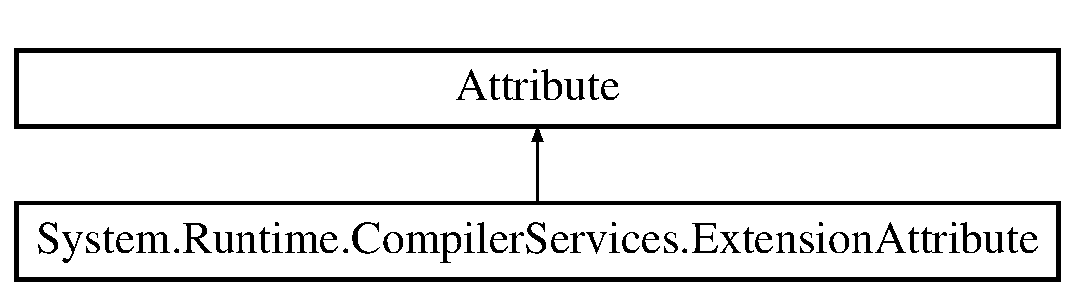
\includegraphics[height=2.000000cm]{class_system_1_1_runtime_1_1_compiler_services_1_1_extension_attribute}
\end{center}
\end{figure}


\subsection{详细描述}


在文件 Tree\-Item.\-cs 第 34 行定义.



该类的文档由以下文件生成\-:\begin{DoxyCompactItemize}
\item 
D\-:/\-My\-Data/\-My\-Git/\-Git\-Hub/\-X\-C\-L\-Net\-Tools/\-X\-C\-L\-Net\-Tools/\-Entity/\-Easy\-U\-I/\hyperlink{_tree_item_8cs}{Tree\-Item.\-cs}\end{DoxyCompactItemize}

\hypertarget{class_x_c_l_net_tools_1_1_entity_1_1_file_info_entity}{}\section{X\+C\+L\+Net\+Tools.\+Entity.\+File\+Info\+Entity类 参考}
\label{class_x_c_l_net_tools_1_1_entity_1_1_file_info_entity}\index{X\+C\+L\+Net\+Tools.\+Entity.\+File\+Info\+Entity@{X\+C\+L\+Net\+Tools.\+Entity.\+File\+Info\+Entity}}


文件信息实体  


\subsection*{属性}
\begin{DoxyCompactItemize}
\item 
int \hyperlink{class_x_c_l_net_tools_1_1_entity_1_1_file_info_entity_a150f26081f12badeea9a2255bbea6faf}{ID}\hspace{0.3cm}{\ttfamily  \mbox{[}get, set\mbox{]}}
\begin{DoxyCompactList}\small\item\em 标识\+ID \end{DoxyCompactList}\item 
bool \hyperlink{class_x_c_l_net_tools_1_1_entity_1_1_file_info_entity_ad945716535742c01f83dffc2766c0987}{Is\+Folder}\hspace{0.3cm}{\ttfamily  \mbox{[}get, set\mbox{]}}
\begin{DoxyCompactList}\small\item\em 是否为文件夹 \end{DoxyCompactList}\item 
string \hyperlink{class_x_c_l_net_tools_1_1_entity_1_1_file_info_entity_a15a2bb6c738c32250f00604b6636cae4}{Name}\hspace{0.3cm}{\ttfamily  \mbox{[}get, set\mbox{]}}
\begin{DoxyCompactList}\small\item\em 文件名 \end{DoxyCompactList}\item 
string \hyperlink{class_x_c_l_net_tools_1_1_entity_1_1_file_info_entity_a46ccaf5dbcc1154782c0227c83eb54e4}{Ext\+Name}\hspace{0.3cm}{\ttfamily  \mbox{[}get, set\mbox{]}}
\begin{DoxyCompactList}\small\item\em 扩展名(不含小圆点) \end{DoxyCompactList}\item 
string \hyperlink{class_x_c_l_net_tools_1_1_entity_1_1_file_info_entity_a6ef4c659747c605379a43168ae1d64f6}{Root\+Path}\hspace{0.3cm}{\ttfamily  \mbox{[}get, set\mbox{]}}
\begin{DoxyCompactList}\small\item\em 根物理路径 \end{DoxyCompactList}\item 
string \hyperlink{class_x_c_l_net_tools_1_1_entity_1_1_file_info_entity_a67f485c1a1af6205351305756d515e98}{Path}\hspace{0.3cm}{\ttfamily  \mbox{[}get, set\mbox{]}}
\begin{DoxyCompactList}\small\item\em 该文件或文件夹的物理路径 \end{DoxyCompactList}\item 
string \hyperlink{class_x_c_l_net_tools_1_1_entity_1_1_file_info_entity_ab93bd802770bb40cc0abdfd35d2fbbc6}{Web\+Path}\hspace{0.3cm}{\ttfamily  \mbox{[}get, set\mbox{]}}
\begin{DoxyCompactList}\small\item\em 该文件或文件夹的web路径 \end{DoxyCompactList}\item 
string \hyperlink{class_x_c_l_net_tools_1_1_entity_1_1_file_info_entity_a795982d186fa2d1ef0e3fb51705f36b2}{Relative\+Path}\hspace{0.3cm}{\ttfamily  \mbox{[}get, set\mbox{]}}
\begin{DoxyCompactList}\small\item\em 该文件或文件夹相对于\+Root\+Path的相对路径 \end{DoxyCompactList}\item 
long \hyperlink{class_x_c_l_net_tools_1_1_entity_1_1_file_info_entity_a7447a43994e75793388e160a626ba346}{Size}\hspace{0.3cm}{\ttfamily  \mbox{[}get, set\mbox{]}}
\begin{DoxyCompactList}\small\item\em 大小(byte) \end{DoxyCompactList}\item 
Date\+Time \hyperlink{class_x_c_l_net_tools_1_1_entity_1_1_file_info_entity_a64c6633bec7e4d547632c122dbaad9f8}{Modify\+Time}\hspace{0.3cm}{\ttfamily  \mbox{[}get, set\mbox{]}}
\begin{DoxyCompactList}\small\item\em 修改时间 \end{DoxyCompactList}\item 
Date\+Time \hyperlink{class_x_c_l_net_tools_1_1_entity_1_1_file_info_entity_a93fc7b2a3119885d9449d1817e7306ca}{Create\+Time}\hspace{0.3cm}{\ttfamily  \mbox{[}get, set\mbox{]}}
\begin{DoxyCompactList}\small\item\em 创建时间 \end{DoxyCompactList}\end{DoxyCompactItemize}


\subsection{详细描述}
文件信息实体 



在文件 File\+Info\+Entity.\+cs 第 17 行定义.



\subsection{属性说明}
\index{X\+C\+L\+Net\+Tools\+::\+Entity\+::\+File\+Info\+Entity@{X\+C\+L\+Net\+Tools\+::\+Entity\+::\+File\+Info\+Entity}!Create\+Time@{Create\+Time}}
\index{Create\+Time@{Create\+Time}!X\+C\+L\+Net\+Tools\+::\+Entity\+::\+File\+Info\+Entity@{X\+C\+L\+Net\+Tools\+::\+Entity\+::\+File\+Info\+Entity}}
\subsubsection[{\texorpdfstring{Create\+Time}{CreateTime}}]{\setlength{\rightskip}{0pt plus 5cm}Date\+Time X\+C\+L\+Net\+Tools.\+Entity.\+File\+Info\+Entity.\+Create\+Time\hspace{0.3cm}{\ttfamily [get]}, {\ttfamily [set]}}\hypertarget{class_x_c_l_net_tools_1_1_entity_1_1_file_info_entity_a93fc7b2a3119885d9449d1817e7306ca}{}\label{class_x_c_l_net_tools_1_1_entity_1_1_file_info_entity_a93fc7b2a3119885d9449d1817e7306ca}


创建时间 



在文件 File\+Info\+Entity.\+cs 第 72 行定义.

\index{X\+C\+L\+Net\+Tools\+::\+Entity\+::\+File\+Info\+Entity@{X\+C\+L\+Net\+Tools\+::\+Entity\+::\+File\+Info\+Entity}!Ext\+Name@{Ext\+Name}}
\index{Ext\+Name@{Ext\+Name}!X\+C\+L\+Net\+Tools\+::\+Entity\+::\+File\+Info\+Entity@{X\+C\+L\+Net\+Tools\+::\+Entity\+::\+File\+Info\+Entity}}
\subsubsection[{\texorpdfstring{Ext\+Name}{ExtName}}]{\setlength{\rightskip}{0pt plus 5cm}string X\+C\+L\+Net\+Tools.\+Entity.\+File\+Info\+Entity.\+Ext\+Name\hspace{0.3cm}{\ttfamily [get]}, {\ttfamily [set]}}\hypertarget{class_x_c_l_net_tools_1_1_entity_1_1_file_info_entity_a46ccaf5dbcc1154782c0227c83eb54e4}{}\label{class_x_c_l_net_tools_1_1_entity_1_1_file_info_entity_a46ccaf5dbcc1154782c0227c83eb54e4}


扩展名(不含小圆点) 



在文件 File\+Info\+Entity.\+cs 第 37 行定义.

\index{X\+C\+L\+Net\+Tools\+::\+Entity\+::\+File\+Info\+Entity@{X\+C\+L\+Net\+Tools\+::\+Entity\+::\+File\+Info\+Entity}!ID@{ID}}
\index{ID@{ID}!X\+C\+L\+Net\+Tools\+::\+Entity\+::\+File\+Info\+Entity@{X\+C\+L\+Net\+Tools\+::\+Entity\+::\+File\+Info\+Entity}}
\subsubsection[{\texorpdfstring{ID}{ID}}]{\setlength{\rightskip}{0pt plus 5cm}int X\+C\+L\+Net\+Tools.\+Entity.\+File\+Info\+Entity.\+ID\hspace{0.3cm}{\ttfamily [get]}, {\ttfamily [set]}}\hypertarget{class_x_c_l_net_tools_1_1_entity_1_1_file_info_entity_a150f26081f12badeea9a2255bbea6faf}{}\label{class_x_c_l_net_tools_1_1_entity_1_1_file_info_entity_a150f26081f12badeea9a2255bbea6faf}


标识\+ID 



在文件 File\+Info\+Entity.\+cs 第 22 行定义.

\index{X\+C\+L\+Net\+Tools\+::\+Entity\+::\+File\+Info\+Entity@{X\+C\+L\+Net\+Tools\+::\+Entity\+::\+File\+Info\+Entity}!Is\+Folder@{Is\+Folder}}
\index{Is\+Folder@{Is\+Folder}!X\+C\+L\+Net\+Tools\+::\+Entity\+::\+File\+Info\+Entity@{X\+C\+L\+Net\+Tools\+::\+Entity\+::\+File\+Info\+Entity}}
\subsubsection[{\texorpdfstring{Is\+Folder}{IsFolder}}]{\setlength{\rightskip}{0pt plus 5cm}bool X\+C\+L\+Net\+Tools.\+Entity.\+File\+Info\+Entity.\+Is\+Folder\hspace{0.3cm}{\ttfamily [get]}, {\ttfamily [set]}}\hypertarget{class_x_c_l_net_tools_1_1_entity_1_1_file_info_entity_ad945716535742c01f83dffc2766c0987}{}\label{class_x_c_l_net_tools_1_1_entity_1_1_file_info_entity_ad945716535742c01f83dffc2766c0987}


是否为文件夹 



在文件 File\+Info\+Entity.\+cs 第 27 行定义.

\index{X\+C\+L\+Net\+Tools\+::\+Entity\+::\+File\+Info\+Entity@{X\+C\+L\+Net\+Tools\+::\+Entity\+::\+File\+Info\+Entity}!Modify\+Time@{Modify\+Time}}
\index{Modify\+Time@{Modify\+Time}!X\+C\+L\+Net\+Tools\+::\+Entity\+::\+File\+Info\+Entity@{X\+C\+L\+Net\+Tools\+::\+Entity\+::\+File\+Info\+Entity}}
\subsubsection[{\texorpdfstring{Modify\+Time}{ModifyTime}}]{\setlength{\rightskip}{0pt plus 5cm}Date\+Time X\+C\+L\+Net\+Tools.\+Entity.\+File\+Info\+Entity.\+Modify\+Time\hspace{0.3cm}{\ttfamily [get]}, {\ttfamily [set]}}\hypertarget{class_x_c_l_net_tools_1_1_entity_1_1_file_info_entity_a64c6633bec7e4d547632c122dbaad9f8}{}\label{class_x_c_l_net_tools_1_1_entity_1_1_file_info_entity_a64c6633bec7e4d547632c122dbaad9f8}


修改时间 



在文件 File\+Info\+Entity.\+cs 第 67 行定义.

\index{X\+C\+L\+Net\+Tools\+::\+Entity\+::\+File\+Info\+Entity@{X\+C\+L\+Net\+Tools\+::\+Entity\+::\+File\+Info\+Entity}!Name@{Name}}
\index{Name@{Name}!X\+C\+L\+Net\+Tools\+::\+Entity\+::\+File\+Info\+Entity@{X\+C\+L\+Net\+Tools\+::\+Entity\+::\+File\+Info\+Entity}}
\subsubsection[{\texorpdfstring{Name}{Name}}]{\setlength{\rightskip}{0pt plus 5cm}string X\+C\+L\+Net\+Tools.\+Entity.\+File\+Info\+Entity.\+Name\hspace{0.3cm}{\ttfamily [get]}, {\ttfamily [set]}}\hypertarget{class_x_c_l_net_tools_1_1_entity_1_1_file_info_entity_a15a2bb6c738c32250f00604b6636cae4}{}\label{class_x_c_l_net_tools_1_1_entity_1_1_file_info_entity_a15a2bb6c738c32250f00604b6636cae4}


文件名 



在文件 File\+Info\+Entity.\+cs 第 32 行定义.

\index{X\+C\+L\+Net\+Tools\+::\+Entity\+::\+File\+Info\+Entity@{X\+C\+L\+Net\+Tools\+::\+Entity\+::\+File\+Info\+Entity}!Path@{Path}}
\index{Path@{Path}!X\+C\+L\+Net\+Tools\+::\+Entity\+::\+File\+Info\+Entity@{X\+C\+L\+Net\+Tools\+::\+Entity\+::\+File\+Info\+Entity}}
\subsubsection[{\texorpdfstring{Path}{Path}}]{\setlength{\rightskip}{0pt plus 5cm}string X\+C\+L\+Net\+Tools.\+Entity.\+File\+Info\+Entity.\+Path\hspace{0.3cm}{\ttfamily [get]}, {\ttfamily [set]}}\hypertarget{class_x_c_l_net_tools_1_1_entity_1_1_file_info_entity_a67f485c1a1af6205351305756d515e98}{}\label{class_x_c_l_net_tools_1_1_entity_1_1_file_info_entity_a67f485c1a1af6205351305756d515e98}


该文件或文件夹的物理路径 



在文件 File\+Info\+Entity.\+cs 第 47 行定义.

\index{X\+C\+L\+Net\+Tools\+::\+Entity\+::\+File\+Info\+Entity@{X\+C\+L\+Net\+Tools\+::\+Entity\+::\+File\+Info\+Entity}!Relative\+Path@{Relative\+Path}}
\index{Relative\+Path@{Relative\+Path}!X\+C\+L\+Net\+Tools\+::\+Entity\+::\+File\+Info\+Entity@{X\+C\+L\+Net\+Tools\+::\+Entity\+::\+File\+Info\+Entity}}
\subsubsection[{\texorpdfstring{Relative\+Path}{RelativePath}}]{\setlength{\rightskip}{0pt plus 5cm}string X\+C\+L\+Net\+Tools.\+Entity.\+File\+Info\+Entity.\+Relative\+Path\hspace{0.3cm}{\ttfamily [get]}, {\ttfamily [set]}}\hypertarget{class_x_c_l_net_tools_1_1_entity_1_1_file_info_entity_a795982d186fa2d1ef0e3fb51705f36b2}{}\label{class_x_c_l_net_tools_1_1_entity_1_1_file_info_entity_a795982d186fa2d1ef0e3fb51705f36b2}


该文件或文件夹相对于\+Root\+Path的相对路径 



在文件 File\+Info\+Entity.\+cs 第 57 行定义.

\index{X\+C\+L\+Net\+Tools\+::\+Entity\+::\+File\+Info\+Entity@{X\+C\+L\+Net\+Tools\+::\+Entity\+::\+File\+Info\+Entity}!Root\+Path@{Root\+Path}}
\index{Root\+Path@{Root\+Path}!X\+C\+L\+Net\+Tools\+::\+Entity\+::\+File\+Info\+Entity@{X\+C\+L\+Net\+Tools\+::\+Entity\+::\+File\+Info\+Entity}}
\subsubsection[{\texorpdfstring{Root\+Path}{RootPath}}]{\setlength{\rightskip}{0pt plus 5cm}string X\+C\+L\+Net\+Tools.\+Entity.\+File\+Info\+Entity.\+Root\+Path\hspace{0.3cm}{\ttfamily [get]}, {\ttfamily [set]}}\hypertarget{class_x_c_l_net_tools_1_1_entity_1_1_file_info_entity_a6ef4c659747c605379a43168ae1d64f6}{}\label{class_x_c_l_net_tools_1_1_entity_1_1_file_info_entity_a6ef4c659747c605379a43168ae1d64f6}


根物理路径 



在文件 File\+Info\+Entity.\+cs 第 42 行定义.

\index{X\+C\+L\+Net\+Tools\+::\+Entity\+::\+File\+Info\+Entity@{X\+C\+L\+Net\+Tools\+::\+Entity\+::\+File\+Info\+Entity}!Size@{Size}}
\index{Size@{Size}!X\+C\+L\+Net\+Tools\+::\+Entity\+::\+File\+Info\+Entity@{X\+C\+L\+Net\+Tools\+::\+Entity\+::\+File\+Info\+Entity}}
\subsubsection[{\texorpdfstring{Size}{Size}}]{\setlength{\rightskip}{0pt plus 5cm}long X\+C\+L\+Net\+Tools.\+Entity.\+File\+Info\+Entity.\+Size\hspace{0.3cm}{\ttfamily [get]}, {\ttfamily [set]}}\hypertarget{class_x_c_l_net_tools_1_1_entity_1_1_file_info_entity_a7447a43994e75793388e160a626ba346}{}\label{class_x_c_l_net_tools_1_1_entity_1_1_file_info_entity_a7447a43994e75793388e160a626ba346}


大小(byte) 



在文件 File\+Info\+Entity.\+cs 第 62 行定义.

\index{X\+C\+L\+Net\+Tools\+::\+Entity\+::\+File\+Info\+Entity@{X\+C\+L\+Net\+Tools\+::\+Entity\+::\+File\+Info\+Entity}!Web\+Path@{Web\+Path}}
\index{Web\+Path@{Web\+Path}!X\+C\+L\+Net\+Tools\+::\+Entity\+::\+File\+Info\+Entity@{X\+C\+L\+Net\+Tools\+::\+Entity\+::\+File\+Info\+Entity}}
\subsubsection[{\texorpdfstring{Web\+Path}{WebPath}}]{\setlength{\rightskip}{0pt plus 5cm}string X\+C\+L\+Net\+Tools.\+Entity.\+File\+Info\+Entity.\+Web\+Path\hspace{0.3cm}{\ttfamily [get]}, {\ttfamily [set]}}\hypertarget{class_x_c_l_net_tools_1_1_entity_1_1_file_info_entity_ab93bd802770bb40cc0abdfd35d2fbbc6}{}\label{class_x_c_l_net_tools_1_1_entity_1_1_file_info_entity_ab93bd802770bb40cc0abdfd35d2fbbc6}


该文件或文件夹的web路径 



在文件 File\+Info\+Entity.\+cs 第 52 行定义.



该类的文档由以下文件生成\+:\begin{DoxyCompactItemize}
\item 
E\+:/\+Git\+Hub/\+X\+C\+L\+Net\+Tools/\+X\+C\+L\+Net\+Tools/\+Entity/\hyperlink{_file_info_entity_8cs}{File\+Info\+Entity.\+cs}\end{DoxyCompactItemize}

\hypertarget{class_x_c_l_net_tools_1_1_f_t_p_1_1_f_t_p_client}{\section{X\-C\-L\-Net\-Tools.\-F\-T\-P.\-F\-T\-P\-Client类 参考}
\label{class_x_c_l_net_tools_1_1_f_t_p_1_1_f_t_p_client}\index{X\-C\-L\-Net\-Tools.\-F\-T\-P.\-F\-T\-P\-Client@{X\-C\-L\-Net\-Tools.\-F\-T\-P.\-F\-T\-P\-Client}}
}


F\-T\-P操作客户端类 \begin{DoxySeeAlso}{参见}
http\-://www.\-cnblogs.\-com/sufei/archive/2012/12/09/2810197.\-html


\end{DoxySeeAlso}
 


\subsection*{Public 类型}
\begin{DoxyCompactItemize}
\item 
enum \hyperlink{class_x_c_l_net_tools_1_1_f_t_p_1_1_f_t_p_client_adef28404af1c916d9bd2bfbfa924b707}{Transfer\-Type} \{ \hyperlink{class_x_c_l_net_tools_1_1_f_t_p_1_1_f_t_p_client_adef28404af1c916d9bd2bfbfa924b707a6ce976e8f061b2b5cfe4d0c50c3405dd}{Transfer\-Type.\-Binary}, 
\hyperlink{class_x_c_l_net_tools_1_1_f_t_p_1_1_f_t_p_client_adef28404af1c916d9bd2bfbfa924b707ad2cd8253361a9c732d21ca1d336599cc}{Transfer\-Type.\-A\-S\-C\-I\-I}
 \}
\begin{DoxyCompactList}\small\item\em 传输模式\-:二进制类型、\-A\-S\-C\-I\-I类型 \end{DoxyCompactList}\end{DoxyCompactItemize}
\subsection*{Public 成员函数}
\begin{DoxyCompactItemize}
\item 
\hyperlink{class_x_c_l_net_tools_1_1_f_t_p_1_1_f_t_p_client_a676653f395ab68c5da43f284bf06a18e}{F\-T\-P\-Client} ()
\begin{DoxyCompactList}\small\item\em 缺省构造函数 \end{DoxyCompactList}\item 
\hyperlink{class_x_c_l_net_tools_1_1_f_t_p_1_1_f_t_p_client_a8ce62cd58f4f1825fcb38503fffd664c}{F\-T\-P\-Client} (string remote\-Host, string remote\-Path, string remote\-User, string remote\-Pass, int remote\-Port)
\begin{DoxyCompactList}\small\item\em 构造函数 \end{DoxyCompactList}\item 
void \hyperlink{class_x_c_l_net_tools_1_1_f_t_p_1_1_f_t_p_client_a80b5588cccdbc0fc599da3b065c17824}{Connect} ()
\begin{DoxyCompactList}\small\item\em 建立连接 \end{DoxyCompactList}\item 
void \hyperlink{class_x_c_l_net_tools_1_1_f_t_p_1_1_f_t_p_client_a68ed147abe1a9c0425e7168b37519979}{Dis\-Connect} ()
\begin{DoxyCompactList}\small\item\em 关闭连接 \end{DoxyCompactList}\item 
void \hyperlink{class_x_c_l_net_tools_1_1_f_t_p_1_1_f_t_p_client_a34ec9858385eb10edb576ee871a0e02f}{Set\-Transfer\-Type} (\hyperlink{class_x_c_l_net_tools_1_1_f_t_p_1_1_f_t_p_client_adef28404af1c916d9bd2bfbfa924b707}{Transfer\-Type} tt\-Type)
\begin{DoxyCompactList}\small\item\em 设置传输模式 \end{DoxyCompactList}\item 
\hyperlink{class_x_c_l_net_tools_1_1_f_t_p_1_1_f_t_p_client_adef28404af1c916d9bd2bfbfa924b707}{Transfer\-Type} \hyperlink{class_x_c_l_net_tools_1_1_f_t_p_1_1_f_t_p_client_abc5c0e7353bbbf20f1dcc1ee2f5d5c3f}{Get\-Transfer\-Type} ()
\begin{DoxyCompactList}\small\item\em 获得传输模式 \end{DoxyCompactList}\item 
string\mbox{[}$\,$\mbox{]} \hyperlink{class_x_c_l_net_tools_1_1_f_t_p_1_1_f_t_p_client_a9563c1fa35e755073b9b279caaf7e354}{Dir} (string str\-Mask)
\begin{DoxyCompactList}\small\item\em 获得文件列表 \end{DoxyCompactList}\item 
void \hyperlink{class_x_c_l_net_tools_1_1_f_t_p_1_1_f_t_p_client_a502eb52b0575947170695c4fcbccc10a}{new\-Put\-By\-Guid} (string str\-File\-Name, string str\-Guid)
\item 
long \hyperlink{class_x_c_l_net_tools_1_1_f_t_p_1_1_f_t_p_client_a39be7d18214835a62484226fc12e2061}{Get\-File\-Size} (string str\-File\-Name)
\begin{DoxyCompactList}\small\item\em 获取文件大小 \end{DoxyCompactList}\item 
string \hyperlink{class_x_c_l_net_tools_1_1_f_t_p_1_1_f_t_p_client_abcdeced5a90923ad5788251d4012694f}{Get\-File\-Info} (string str\-File\-Name)
\begin{DoxyCompactList}\small\item\em 获取文件信息 \end{DoxyCompactList}\item 
void \hyperlink{class_x_c_l_net_tools_1_1_f_t_p_1_1_f_t_p_client_a1be296574d7342283c236d8b51ca2b04}{Delete} (string str\-File\-Name)
\begin{DoxyCompactList}\small\item\em 删除 \end{DoxyCompactList}\item 
void \hyperlink{class_x_c_l_net_tools_1_1_f_t_p_1_1_f_t_p_client_aaadb1ae86c64e8ec958e8333fc6b9bce}{Rename} (string str\-Old\-File\-Name, string str\-New\-File\-Name)
\begin{DoxyCompactList}\small\item\em 重命名(如果新文件名与已有文件重名,将覆盖已有文件) \end{DoxyCompactList}\item 
void \hyperlink{class_x_c_l_net_tools_1_1_f_t_p_1_1_f_t_p_client_a67852a51f561336c777b896af2e95990}{Get} (string str\-File\-Name\-Mask, string str\-Folder)
\begin{DoxyCompactList}\small\item\em 下载一批文件 \end{DoxyCompactList}\item 
void \hyperlink{class_x_c_l_net_tools_1_1_f_t_p_1_1_f_t_p_client_a87ce6305af9ccb5e04b0669bd0eac812}{Get} (string str\-Remote\-File\-Name, string str\-Folder, string str\-Local\-File\-Name)
\begin{DoxyCompactList}\small\item\em 下载一个文件 \end{DoxyCompactList}\item 
void \hyperlink{class_x_c_l_net_tools_1_1_f_t_p_1_1_f_t_p_client_a7648a7d3ce55e3332618aca711c3d6ea}{Get\-No\-Binary} (string str\-Remote\-File\-Name, string str\-Folder, string str\-Local\-File\-Name)
\begin{DoxyCompactList}\small\item\em 下载一个文件 \end{DoxyCompactList}\item 
void \hyperlink{class_x_c_l_net_tools_1_1_f_t_p_1_1_f_t_p_client_aa610dab6dd9699203f7d4da488b3ca20}{Put} (string str\-Folder, string str\-File\-Name\-Mask)
\begin{DoxyCompactList}\small\item\em 上传一批文件 \end{DoxyCompactList}\item 
void \hyperlink{class_x_c_l_net_tools_1_1_f_t_p_1_1_f_t_p_client_a0ce0fbef1a6c4a2c872315c104f8fd62}{Put} (string str\-File\-Name)
\begin{DoxyCompactList}\small\item\em 上传一个文件 \end{DoxyCompactList}\item 
void \hyperlink{class_x_c_l_net_tools_1_1_f_t_p_1_1_f_t_p_client_a9f333aedd5467c2fdc46d33298dc9dbb}{Put\-By\-Guid} (string str\-File\-Name, string str\-Guid)
\begin{DoxyCompactList}\small\item\em 上传一个文件 \end{DoxyCompactList}\item 
void \hyperlink{class_x_c_l_net_tools_1_1_f_t_p_1_1_f_t_p_client_aaf6ecfb2034736ffe5f88945ec873efe}{Mk\-Dir} (string str\-Dir\-Name)
\begin{DoxyCompactList}\small\item\em 创建目录 \end{DoxyCompactList}\item 
void \hyperlink{class_x_c_l_net_tools_1_1_f_t_p_1_1_f_t_p_client_a4c4167a6afd00ed6e1f5303e59555037}{Rm\-Dir} (string str\-Dir\-Name)
\begin{DoxyCompactList}\small\item\em 删除目录 \end{DoxyCompactList}\item 
void \hyperlink{class_x_c_l_net_tools_1_1_f_t_p_1_1_f_t_p_client_a6345c0af7cd414503395170157d0db3b}{Ch\-Dir} (string str\-Dir\-Name)
\begin{DoxyCompactList}\small\item\em 改变目录 \end{DoxyCompactList}\item 
void \hyperlink{class_x_c_l_net_tools_1_1_f_t_p_1_1_f_t_p_client_af99f1f4bd038882ec30bdf4e89d73d4a}{Send\-Command} (String str\-Command)
\begin{DoxyCompactList}\small\item\em 发送命令并获取应答码和最后一行应答字符串 \end{DoxyCompactList}\end{DoxyCompactItemize}
\subsection*{属性}
\begin{DoxyCompactItemize}
\item 
string \hyperlink{class_x_c_l_net_tools_1_1_f_t_p_1_1_f_t_p_client_a020891b3ab32deba2b8e2b2204349f1d}{Remote\-Host}\hspace{0.3cm}{\ttfamily  \mbox{[}get, set\mbox{]}}
\begin{DoxyCompactList}\small\item\em F\-T\-P服务器\-I\-P地址 \end{DoxyCompactList}\item 
int \hyperlink{class_x_c_l_net_tools_1_1_f_t_p_1_1_f_t_p_client_af47bf07406237f3bd179472debf9c84d}{Remote\-Port}\hspace{0.3cm}{\ttfamily  \mbox{[}get, set\mbox{]}}
\begin{DoxyCompactList}\small\item\em F\-T\-P服务器端口 \end{DoxyCompactList}\item 
string \hyperlink{class_x_c_l_net_tools_1_1_f_t_p_1_1_f_t_p_client_a6dd534c17624097f4c29442ce3e5a176}{Remote\-Path}\hspace{0.3cm}{\ttfamily  \mbox{[}get, set\mbox{]}}
\begin{DoxyCompactList}\small\item\em 当前服务器目录 \end{DoxyCompactList}\item 
string \hyperlink{class_x_c_l_net_tools_1_1_f_t_p_1_1_f_t_p_client_ab97c698dca9a54f44b1e69cb15c1126d}{Remote\-User}\hspace{0.3cm}{\ttfamily  \mbox{[}set\mbox{]}}
\begin{DoxyCompactList}\small\item\em 登录用户账号 \end{DoxyCompactList}\item 
string \hyperlink{class_x_c_l_net_tools_1_1_f_t_p_1_1_f_t_p_client_a89a0c18691dfde35bdb46696a0344bff}{Remote\-Pass}\hspace{0.3cm}{\ttfamily  \mbox{[}set\mbox{]}}
\begin{DoxyCompactList}\small\item\em 用户登录密码 \end{DoxyCompactList}\item 
bool \hyperlink{class_x_c_l_net_tools_1_1_f_t_p_1_1_f_t_p_client_af3e0775ddf1dc1530b82b5b0a6aa4d25}{Connected}\hspace{0.3cm}{\ttfamily  \mbox{[}get\mbox{]}}
\begin{DoxyCompactList}\small\item\em 是否登录 \end{DoxyCompactList}\end{DoxyCompactItemize}


\subsection{详细描述}
F\-T\-P操作客户端类 \begin{DoxySeeAlso}{参见}
http\-://www.\-cnblogs.\-com/sufei/archive/2012/12/09/2810197.\-html


\end{DoxySeeAlso}




在文件 F\-T\-P\-Client.\-cs 第 22 行定义.



\subsection{成员枚举类型说明}
\hypertarget{class_x_c_l_net_tools_1_1_f_t_p_1_1_f_t_p_client_adef28404af1c916d9bd2bfbfa924b707}{\index{X\-C\-L\-Net\-Tools\-::\-F\-T\-P\-::\-F\-T\-P\-Client@{X\-C\-L\-Net\-Tools\-::\-F\-T\-P\-::\-F\-T\-P\-Client}!Transfer\-Type@{Transfer\-Type}}
\index{Transfer\-Type@{Transfer\-Type}!XCLNetTools::FTP::FTPClient@{X\-C\-L\-Net\-Tools\-::\-F\-T\-P\-::\-F\-T\-P\-Client}}
\subsubsection[{Transfer\-Type}]{\setlength{\rightskip}{0pt plus 5cm}enum {\bf X\-C\-L\-Net\-Tools.\-F\-T\-P.\-F\-T\-P\-Client.\-Transfer\-Type}}}\label{class_x_c_l_net_tools_1_1_f_t_p_1_1_f_t_p_client_adef28404af1c916d9bd2bfbfa924b707}


传输模式\-:二进制类型、\-A\-S\-C\-I\-I类型 

\begin{Desc}
\item[枚举值]\par
\begin{description}
\index{Binary@{Binary}!X\-C\-L\-Net\-Tools\-::\-F\-T\-P\-::\-F\-T\-P\-Client@{X\-C\-L\-Net\-Tools\-::\-F\-T\-P\-::\-F\-T\-P\-Client}}\index{X\-C\-L\-Net\-Tools\-::\-F\-T\-P\-::\-F\-T\-P\-Client@{X\-C\-L\-Net\-Tools\-::\-F\-T\-P\-::\-F\-T\-P\-Client}!Binary@{Binary}}\item[{\em 
\hypertarget{class_x_c_l_net_tools_1_1_f_t_p_1_1_f_t_p_client_adef28404af1c916d9bd2bfbfa924b707a6ce976e8f061b2b5cfe4d0c50c3405dd}{Binary}\label{class_x_c_l_net_tools_1_1_f_t_p_1_1_f_t_p_client_adef28404af1c916d9bd2bfbfa924b707a6ce976e8f061b2b5cfe4d0c50c3405dd}
}]二进制类型 \index{A\-S\-C\-I\-I@{A\-S\-C\-I\-I}!X\-C\-L\-Net\-Tools\-::\-F\-T\-P\-::\-F\-T\-P\-Client@{X\-C\-L\-Net\-Tools\-::\-F\-T\-P\-::\-F\-T\-P\-Client}}\index{X\-C\-L\-Net\-Tools\-::\-F\-T\-P\-::\-F\-T\-P\-Client@{X\-C\-L\-Net\-Tools\-::\-F\-T\-P\-::\-F\-T\-P\-Client}!A\-S\-C\-I\-I@{A\-S\-C\-I\-I}}\item[{\em 
\hypertarget{class_x_c_l_net_tools_1_1_f_t_p_1_1_f_t_p_client_adef28404af1c916d9bd2bfbfa924b707ad2cd8253361a9c732d21ca1d336599cc}{A\-S\-C\-I\-I}\label{class_x_c_l_net_tools_1_1_f_t_p_1_1_f_t_p_client_adef28404af1c916d9bd2bfbfa924b707ad2cd8253361a9c732d21ca1d336599cc}
}]A\-S\-C\-I\-I类型 \end{description}
\end{Desc}


在文件 F\-T\-P\-Client.\-cs 第 253 行定义.



\subsection{构造及析构函数说明}
\hypertarget{class_x_c_l_net_tools_1_1_f_t_p_1_1_f_t_p_client_a676653f395ab68c5da43f284bf06a18e}{\index{X\-C\-L\-Net\-Tools\-::\-F\-T\-P\-::\-F\-T\-P\-Client@{X\-C\-L\-Net\-Tools\-::\-F\-T\-P\-::\-F\-T\-P\-Client}!F\-T\-P\-Client@{F\-T\-P\-Client}}
\index{F\-T\-P\-Client@{F\-T\-P\-Client}!XCLNetTools::FTP::FTPClient@{X\-C\-L\-Net\-Tools\-::\-F\-T\-P\-::\-F\-T\-P\-Client}}
\subsubsection[{F\-T\-P\-Client}]{\setlength{\rightskip}{0pt plus 5cm}X\-C\-L\-Net\-Tools.\-F\-T\-P.\-F\-T\-P\-Client.\-F\-T\-P\-Client (
\begin{DoxyParamCaption}
{}
\end{DoxyParamCaption}
)}}\label{class_x_c_l_net_tools_1_1_f_t_p_1_1_f_t_p_client_a676653f395ab68c5da43f284bf06a18e}


缺省构造函数 



在文件 F\-T\-P\-Client.\-cs 第 31 行定义.

\hypertarget{class_x_c_l_net_tools_1_1_f_t_p_1_1_f_t_p_client_a8ce62cd58f4f1825fcb38503fffd664c}{\index{X\-C\-L\-Net\-Tools\-::\-F\-T\-P\-::\-F\-T\-P\-Client@{X\-C\-L\-Net\-Tools\-::\-F\-T\-P\-::\-F\-T\-P\-Client}!F\-T\-P\-Client@{F\-T\-P\-Client}}
\index{F\-T\-P\-Client@{F\-T\-P\-Client}!XCLNetTools::FTP::FTPClient@{X\-C\-L\-Net\-Tools\-::\-F\-T\-P\-::\-F\-T\-P\-Client}}
\subsubsection[{F\-T\-P\-Client}]{\setlength{\rightskip}{0pt plus 5cm}X\-C\-L\-Net\-Tools.\-F\-T\-P.\-F\-T\-P\-Client.\-F\-T\-P\-Client (
\begin{DoxyParamCaption}
\item[{string}]{remote\-Host, }
\item[{string}]{remote\-Path, }
\item[{string}]{remote\-User, }
\item[{string}]{remote\-Pass, }
\item[{int}]{remote\-Port}
\end{DoxyParamCaption}
)}}\label{class_x_c_l_net_tools_1_1_f_t_p_1_1_f_t_p_client_a8ce62cd58f4f1825fcb38503fffd664c}


构造函数 



在文件 F\-T\-P\-Client.\-cs 第 44 行定义.



\subsection{成员函数说明}
\hypertarget{class_x_c_l_net_tools_1_1_f_t_p_1_1_f_t_p_client_a6345c0af7cd414503395170157d0db3b}{\index{X\-C\-L\-Net\-Tools\-::\-F\-T\-P\-::\-F\-T\-P\-Client@{X\-C\-L\-Net\-Tools\-::\-F\-T\-P\-::\-F\-T\-P\-Client}!Ch\-Dir@{Ch\-Dir}}
\index{Ch\-Dir@{Ch\-Dir}!XCLNetTools::FTP::FTPClient@{X\-C\-L\-Net\-Tools\-::\-F\-T\-P\-::\-F\-T\-P\-Client}}
\subsubsection[{Ch\-Dir}]{\setlength{\rightskip}{0pt plus 5cm}void X\-C\-L\-Net\-Tools.\-F\-T\-P.\-F\-T\-P\-Client.\-Ch\-Dir (
\begin{DoxyParamCaption}
\item[{string}]{str\-Dir\-Name}
\end{DoxyParamCaption}
)}}\label{class_x_c_l_net_tools_1_1_f_t_p_1_1_f_t_p_client_a6345c0af7cd414503395170157d0db3b}


改变目录 


\begin{DoxyParams}{参数}
{\em str\-Dir\-Name} & 新的工作目录名\\
\hline
\end{DoxyParams}


在文件 F\-T\-P\-Client.\-cs 第 756 行定义.

\hypertarget{class_x_c_l_net_tools_1_1_f_t_p_1_1_f_t_p_client_a80b5588cccdbc0fc599da3b065c17824}{\index{X\-C\-L\-Net\-Tools\-::\-F\-T\-P\-::\-F\-T\-P\-Client@{X\-C\-L\-Net\-Tools\-::\-F\-T\-P\-::\-F\-T\-P\-Client}!Connect@{Connect}}
\index{Connect@{Connect}!XCLNetTools::FTP::FTPClient@{X\-C\-L\-Net\-Tools\-::\-F\-T\-P\-::\-F\-T\-P\-Client}}
\subsubsection[{Connect}]{\setlength{\rightskip}{0pt plus 5cm}void X\-C\-L\-Net\-Tools.\-F\-T\-P.\-F\-T\-P\-Client.\-Connect (
\begin{DoxyParamCaption}
{}
\end{DoxyParamCaption}
)}}\label{class_x_c_l_net_tools_1_1_f_t_p_1_1_f_t_p_client_a80b5588cccdbc0fc599da3b065c17824}


建立连接 



在文件 F\-T\-P\-Client.\-cs 第 194 行定义.

\hypertarget{class_x_c_l_net_tools_1_1_f_t_p_1_1_f_t_p_client_a1be296574d7342283c236d8b51ca2b04}{\index{X\-C\-L\-Net\-Tools\-::\-F\-T\-P\-::\-F\-T\-P\-Client@{X\-C\-L\-Net\-Tools\-::\-F\-T\-P\-::\-F\-T\-P\-Client}!Delete@{Delete}}
\index{Delete@{Delete}!XCLNetTools::FTP::FTPClient@{X\-C\-L\-Net\-Tools\-::\-F\-T\-P\-::\-F\-T\-P\-Client}}
\subsubsection[{Delete}]{\setlength{\rightskip}{0pt plus 5cm}void X\-C\-L\-Net\-Tools.\-F\-T\-P.\-F\-T\-P\-Client.\-Delete (
\begin{DoxyParamCaption}
\item[{string}]{str\-File\-Name}
\end{DoxyParamCaption}
)}}\label{class_x_c_l_net_tools_1_1_f_t_p_1_1_f_t_p_client_a1be296574d7342283c236d8b51ca2b04}


删除 


\begin{DoxyParams}{参数}
{\em str\-File\-Name} & 待删除文件名\\
\hline
\end{DoxyParams}


在文件 F\-T\-P\-Client.\-cs 第 446 行定义.

\hypertarget{class_x_c_l_net_tools_1_1_f_t_p_1_1_f_t_p_client_a9563c1fa35e755073b9b279caaf7e354}{\index{X\-C\-L\-Net\-Tools\-::\-F\-T\-P\-::\-F\-T\-P\-Client@{X\-C\-L\-Net\-Tools\-::\-F\-T\-P\-::\-F\-T\-P\-Client}!Dir@{Dir}}
\index{Dir@{Dir}!XCLNetTools::FTP::FTPClient@{X\-C\-L\-Net\-Tools\-::\-F\-T\-P\-::\-F\-T\-P\-Client}}
\subsubsection[{Dir}]{\setlength{\rightskip}{0pt plus 5cm}string \mbox{[}$\,$\mbox{]} X\-C\-L\-Net\-Tools.\-F\-T\-P.\-F\-T\-P\-Client.\-Dir (
\begin{DoxyParamCaption}
\item[{string}]{str\-Mask}
\end{DoxyParamCaption}
)}}\label{class_x_c_l_net_tools_1_1_f_t_p_1_1_f_t_p_client_a9563c1fa35e755073b9b279caaf7e354}


获得文件列表 


\begin{DoxyParams}{参数}
{\em str\-Mask} & 文件名的匹配字符串\\
\hline
\end{DoxyParams}


在文件 F\-T\-P\-Client.\-cs 第 307 行定义.

\hypertarget{class_x_c_l_net_tools_1_1_f_t_p_1_1_f_t_p_client_a68ed147abe1a9c0425e7168b37519979}{\index{X\-C\-L\-Net\-Tools\-::\-F\-T\-P\-::\-F\-T\-P\-Client@{X\-C\-L\-Net\-Tools\-::\-F\-T\-P\-::\-F\-T\-P\-Client}!Dis\-Connect@{Dis\-Connect}}
\index{Dis\-Connect@{Dis\-Connect}!XCLNetTools::FTP::FTPClient@{X\-C\-L\-Net\-Tools\-::\-F\-T\-P\-::\-F\-T\-P\-Client}}
\subsubsection[{Dis\-Connect}]{\setlength{\rightskip}{0pt plus 5cm}void X\-C\-L\-Net\-Tools.\-F\-T\-P.\-F\-T\-P\-Client.\-Dis\-Connect (
\begin{DoxyParamCaption}
{}
\end{DoxyParamCaption}
)}}\label{class_x_c_l_net_tools_1_1_f_t_p_1_1_f_t_p_client_a68ed147abe1a9c0425e7168b37519979}


关闭连接 



在文件 F\-T\-P\-Client.\-cs 第 237 行定义.

\hypertarget{class_x_c_l_net_tools_1_1_f_t_p_1_1_f_t_p_client_a67852a51f561336c777b896af2e95990}{\index{X\-C\-L\-Net\-Tools\-::\-F\-T\-P\-::\-F\-T\-P\-Client@{X\-C\-L\-Net\-Tools\-::\-F\-T\-P\-::\-F\-T\-P\-Client}!Get@{Get}}
\index{Get@{Get}!XCLNetTools::FTP::FTPClient@{X\-C\-L\-Net\-Tools\-::\-F\-T\-P\-::\-F\-T\-P\-Client}}
\subsubsection[{Get}]{\setlength{\rightskip}{0pt plus 5cm}void X\-C\-L\-Net\-Tools.\-F\-T\-P.\-F\-T\-P\-Client.\-Get (
\begin{DoxyParamCaption}
\item[{string}]{str\-File\-Name\-Mask, }
\item[{string}]{str\-Folder}
\end{DoxyParamCaption}
)}}\label{class_x_c_l_net_tools_1_1_f_t_p_1_1_f_t_p_client_a67852a51f561336c777b896af2e95990}


下载一批文件 


\begin{DoxyParams}{参数}
{\em str\-File\-Name\-Mask} & 文件名的匹配字符串\\
\hline
{\em str\-Folder} & 本地目录(不得以\textbackslash{}结束)\\
\hline
\end{DoxyParams}


在文件 F\-T\-P\-Client.\-cs 第 492 行定义.

\hypertarget{class_x_c_l_net_tools_1_1_f_t_p_1_1_f_t_p_client_a87ce6305af9ccb5e04b0669bd0eac812}{\index{X\-C\-L\-Net\-Tools\-::\-F\-T\-P\-::\-F\-T\-P\-Client@{X\-C\-L\-Net\-Tools\-::\-F\-T\-P\-::\-F\-T\-P\-Client}!Get@{Get}}
\index{Get@{Get}!XCLNetTools::FTP::FTPClient@{X\-C\-L\-Net\-Tools\-::\-F\-T\-P\-::\-F\-T\-P\-Client}}
\subsubsection[{Get}]{\setlength{\rightskip}{0pt plus 5cm}void X\-C\-L\-Net\-Tools.\-F\-T\-P.\-F\-T\-P\-Client.\-Get (
\begin{DoxyParamCaption}
\item[{string}]{str\-Remote\-File\-Name, }
\item[{string}]{str\-Folder, }
\item[{string}]{str\-Local\-File\-Name}
\end{DoxyParamCaption}
)}}\label{class_x_c_l_net_tools_1_1_f_t_p_1_1_f_t_p_client_a87ce6305af9ccb5e04b0669bd0eac812}


下载一个文件 


\begin{DoxyParams}{参数}
{\em str\-Remote\-File\-Name} & 要下载的文件名\\
\hline
{\em str\-Folder} & 本地目录(不得以\textbackslash{}结束)\\
\hline
{\em str\-Local\-File\-Name} & 保存在本地时的文件名\\
\hline
\end{DoxyParams}


在文件 F\-T\-P\-Client.\-cs 第 514 行定义.

\hypertarget{class_x_c_l_net_tools_1_1_f_t_p_1_1_f_t_p_client_abcdeced5a90923ad5788251d4012694f}{\index{X\-C\-L\-Net\-Tools\-::\-F\-T\-P\-::\-F\-T\-P\-Client@{X\-C\-L\-Net\-Tools\-::\-F\-T\-P\-::\-F\-T\-P\-Client}!Get\-File\-Info@{Get\-File\-Info}}
\index{Get\-File\-Info@{Get\-File\-Info}!XCLNetTools::FTP::FTPClient@{X\-C\-L\-Net\-Tools\-::\-F\-T\-P\-::\-F\-T\-P\-Client}}
\subsubsection[{Get\-File\-Info}]{\setlength{\rightskip}{0pt plus 5cm}string X\-C\-L\-Net\-Tools.\-F\-T\-P.\-F\-T\-P\-Client.\-Get\-File\-Info (
\begin{DoxyParamCaption}
\item[{string}]{str\-File\-Name}
\end{DoxyParamCaption}
)}}\label{class_x_c_l_net_tools_1_1_f_t_p_1_1_f_t_p_client_abcdeced5a90923ad5788251d4012694f}


获取文件信息 


\begin{DoxyParams}{参数}
{\em str\-File\-Name} & 文件名\\
\hline
\end{DoxyParams}
\begin{DoxyReturn}{返回}
文件大小
\end{DoxyReturn}


在文件 F\-T\-P\-Client.\-cs 第 410 行定义.

\hypertarget{class_x_c_l_net_tools_1_1_f_t_p_1_1_f_t_p_client_a39be7d18214835a62484226fc12e2061}{\index{X\-C\-L\-Net\-Tools\-::\-F\-T\-P\-::\-F\-T\-P\-Client@{X\-C\-L\-Net\-Tools\-::\-F\-T\-P\-::\-F\-T\-P\-Client}!Get\-File\-Size@{Get\-File\-Size}}
\index{Get\-File\-Size@{Get\-File\-Size}!XCLNetTools::FTP::FTPClient@{X\-C\-L\-Net\-Tools\-::\-F\-T\-P\-::\-F\-T\-P\-Client}}
\subsubsection[{Get\-File\-Size}]{\setlength{\rightskip}{0pt plus 5cm}long X\-C\-L\-Net\-Tools.\-F\-T\-P.\-F\-T\-P\-Client.\-Get\-File\-Size (
\begin{DoxyParamCaption}
\item[{string}]{str\-File\-Name}
\end{DoxyParamCaption}
)}}\label{class_x_c_l_net_tools_1_1_f_t_p_1_1_f_t_p_client_a39be7d18214835a62484226fc12e2061}


获取文件大小 


\begin{DoxyParams}{参数}
{\em str\-File\-Name} & 文件名\\
\hline
\end{DoxyParams}
\begin{DoxyReturn}{返回}
文件大小
\end{DoxyReturn}


在文件 F\-T\-P\-Client.\-cs 第 386 行定义.

\hypertarget{class_x_c_l_net_tools_1_1_f_t_p_1_1_f_t_p_client_a7648a7d3ce55e3332618aca711c3d6ea}{\index{X\-C\-L\-Net\-Tools\-::\-F\-T\-P\-::\-F\-T\-P\-Client@{X\-C\-L\-Net\-Tools\-::\-F\-T\-P\-::\-F\-T\-P\-Client}!Get\-No\-Binary@{Get\-No\-Binary}}
\index{Get\-No\-Binary@{Get\-No\-Binary}!XCLNetTools::FTP::FTPClient@{X\-C\-L\-Net\-Tools\-::\-F\-T\-P\-::\-F\-T\-P\-Client}}
\subsubsection[{Get\-No\-Binary}]{\setlength{\rightskip}{0pt plus 5cm}void X\-C\-L\-Net\-Tools.\-F\-T\-P.\-F\-T\-P\-Client.\-Get\-No\-Binary (
\begin{DoxyParamCaption}
\item[{string}]{str\-Remote\-File\-Name, }
\item[{string}]{str\-Folder, }
\item[{string}]{str\-Local\-File\-Name}
\end{DoxyParamCaption}
)}}\label{class_x_c_l_net_tools_1_1_f_t_p_1_1_f_t_p_client_a7648a7d3ce55e3332618aca711c3d6ea}


下载一个文件 


\begin{DoxyParams}{参数}
{\em str\-Remote\-File\-Name} & 要下载的文件名\\
\hline
{\em str\-Folder} & 本地目录(不得以\textbackslash{}结束)\\
\hline
{\em str\-Local\-File\-Name} & 保存在本地时的文件名\\
\hline
\end{DoxyParams}


在文件 F\-T\-P\-Client.\-cs 第 573 行定义.

\hypertarget{class_x_c_l_net_tools_1_1_f_t_p_1_1_f_t_p_client_abc5c0e7353bbbf20f1dcc1ee2f5d5c3f}{\index{X\-C\-L\-Net\-Tools\-::\-F\-T\-P\-::\-F\-T\-P\-Client@{X\-C\-L\-Net\-Tools\-::\-F\-T\-P\-::\-F\-T\-P\-Client}!Get\-Transfer\-Type@{Get\-Transfer\-Type}}
\index{Get\-Transfer\-Type@{Get\-Transfer\-Type}!XCLNetTools::FTP::FTPClient@{X\-C\-L\-Net\-Tools\-::\-F\-T\-P\-::\-F\-T\-P\-Client}}
\subsubsection[{Get\-Transfer\-Type}]{\setlength{\rightskip}{0pt plus 5cm}{\bf Transfer\-Type} X\-C\-L\-Net\-Tools.\-F\-T\-P.\-F\-T\-P\-Client.\-Get\-Transfer\-Type (
\begin{DoxyParamCaption}
{}
\end{DoxyParamCaption}
)}}\label{class_x_c_l_net_tools_1_1_f_t_p_1_1_f_t_p_client_abc5c0e7353bbbf20f1dcc1ee2f5d5c3f}


获得传输模式 

\begin{DoxyReturn}{返回}
传输模式
\end{DoxyReturn}


在文件 F\-T\-P\-Client.\-cs 第 294 行定义.

\hypertarget{class_x_c_l_net_tools_1_1_f_t_p_1_1_f_t_p_client_aaf6ecfb2034736ffe5f88945ec873efe}{\index{X\-C\-L\-Net\-Tools\-::\-F\-T\-P\-::\-F\-T\-P\-Client@{X\-C\-L\-Net\-Tools\-::\-F\-T\-P\-::\-F\-T\-P\-Client}!Mk\-Dir@{Mk\-Dir}}
\index{Mk\-Dir@{Mk\-Dir}!XCLNetTools::FTP::FTPClient@{X\-C\-L\-Net\-Tools\-::\-F\-T\-P\-::\-F\-T\-P\-Client}}
\subsubsection[{Mk\-Dir}]{\setlength{\rightskip}{0pt plus 5cm}void X\-C\-L\-Net\-Tools.\-F\-T\-P.\-F\-T\-P\-Client.\-Mk\-Dir (
\begin{DoxyParamCaption}
\item[{string}]{str\-Dir\-Name}
\end{DoxyParamCaption}
)}}\label{class_x_c_l_net_tools_1_1_f_t_p_1_1_f_t_p_client_aaf6ecfb2034736ffe5f88945ec873efe}


创建目录 


\begin{DoxyParams}{参数}
{\em str\-Dir\-Name} & 目录名\\
\hline
\end{DoxyParams}


在文件 F\-T\-P\-Client.\-cs 第 722 行定义.

\hypertarget{class_x_c_l_net_tools_1_1_f_t_p_1_1_f_t_p_client_a502eb52b0575947170695c4fcbccc10a}{\index{X\-C\-L\-Net\-Tools\-::\-F\-T\-P\-::\-F\-T\-P\-Client@{X\-C\-L\-Net\-Tools\-::\-F\-T\-P\-::\-F\-T\-P\-Client}!new\-Put\-By\-Guid@{new\-Put\-By\-Guid}}
\index{new\-Put\-By\-Guid@{new\-Put\-By\-Guid}!XCLNetTools::FTP::FTPClient@{X\-C\-L\-Net\-Tools\-::\-F\-T\-P\-::\-F\-T\-P\-Client}}
\subsubsection[{new\-Put\-By\-Guid}]{\setlength{\rightskip}{0pt plus 5cm}void X\-C\-L\-Net\-Tools.\-F\-T\-P.\-F\-T\-P\-Client.\-new\-Put\-By\-Guid (
\begin{DoxyParamCaption}
\item[{string}]{str\-File\-Name, }
\item[{string}]{str\-Guid}
\end{DoxyParamCaption}
)}}\label{class_x_c_l_net_tools_1_1_f_t_p_1_1_f_t_p_client_a502eb52b0575947170695c4fcbccc10a}


在文件 F\-T\-P\-Client.\-cs 第 344 行定义.

\hypertarget{class_x_c_l_net_tools_1_1_f_t_p_1_1_f_t_p_client_aa610dab6dd9699203f7d4da488b3ca20}{\index{X\-C\-L\-Net\-Tools\-::\-F\-T\-P\-::\-F\-T\-P\-Client@{X\-C\-L\-Net\-Tools\-::\-F\-T\-P\-::\-F\-T\-P\-Client}!Put@{Put}}
\index{Put@{Put}!XCLNetTools::FTP::FTPClient@{X\-C\-L\-Net\-Tools\-::\-F\-T\-P\-::\-F\-T\-P\-Client}}
\subsubsection[{Put}]{\setlength{\rightskip}{0pt plus 5cm}void X\-C\-L\-Net\-Tools.\-F\-T\-P.\-F\-T\-P\-Client.\-Put (
\begin{DoxyParamCaption}
\item[{string}]{str\-Folder, }
\item[{string}]{str\-File\-Name\-Mask}
\end{DoxyParamCaption}
)}}\label{class_x_c_l_net_tools_1_1_f_t_p_1_1_f_t_p_client_aa610dab6dd9699203f7d4da488b3ca20}


上传一批文件 


\begin{DoxyParams}{参数}
{\em str\-Folder} & 本地目录(不得以\textbackslash{}结束)\\
\hline
{\em str\-File\-Name\-Mask} & 文件名匹配字符(可以包含$\ast$和?)\\
\hline
\end{DoxyParams}


在文件 F\-T\-P\-Client.\-cs 第 620 行定义.

\hypertarget{class_x_c_l_net_tools_1_1_f_t_p_1_1_f_t_p_client_a0ce0fbef1a6c4a2c872315c104f8fd62}{\index{X\-C\-L\-Net\-Tools\-::\-F\-T\-P\-::\-F\-T\-P\-Client@{X\-C\-L\-Net\-Tools\-::\-F\-T\-P\-::\-F\-T\-P\-Client}!Put@{Put}}
\index{Put@{Put}!XCLNetTools::FTP::FTPClient@{X\-C\-L\-Net\-Tools\-::\-F\-T\-P\-::\-F\-T\-P\-Client}}
\subsubsection[{Put}]{\setlength{\rightskip}{0pt plus 5cm}void X\-C\-L\-Net\-Tools.\-F\-T\-P.\-F\-T\-P\-Client.\-Put (
\begin{DoxyParamCaption}
\item[{string}]{str\-File\-Name}
\end{DoxyParamCaption}
)}}\label{class_x_c_l_net_tools_1_1_f_t_p_1_1_f_t_p_client_a0ce0fbef1a6c4a2c872315c104f8fd62}


上传一个文件 


\begin{DoxyParams}{参数}
{\em str\-File\-Name} & 本地文件名\\
\hline
\end{DoxyParams}


在文件 F\-T\-P\-Client.\-cs 第 633 行定义.

\hypertarget{class_x_c_l_net_tools_1_1_f_t_p_1_1_f_t_p_client_a9f333aedd5467c2fdc46d33298dc9dbb}{\index{X\-C\-L\-Net\-Tools\-::\-F\-T\-P\-::\-F\-T\-P\-Client@{X\-C\-L\-Net\-Tools\-::\-F\-T\-P\-::\-F\-T\-P\-Client}!Put\-By\-Guid@{Put\-By\-Guid}}
\index{Put\-By\-Guid@{Put\-By\-Guid}!XCLNetTools::FTP::FTPClient@{X\-C\-L\-Net\-Tools\-::\-F\-T\-P\-::\-F\-T\-P\-Client}}
\subsubsection[{Put\-By\-Guid}]{\setlength{\rightskip}{0pt plus 5cm}void X\-C\-L\-Net\-Tools.\-F\-T\-P.\-F\-T\-P\-Client.\-Put\-By\-Guid (
\begin{DoxyParamCaption}
\item[{string}]{str\-File\-Name, }
\item[{string}]{str\-Guid}
\end{DoxyParamCaption}
)}}\label{class_x_c_l_net_tools_1_1_f_t_p_1_1_f_t_p_client_a9f333aedd5467c2fdc46d33298dc9dbb}


上传一个文件 


\begin{DoxyParams}{参数}
{\em str\-File\-Name} & 本地文件名\\
\hline
\end{DoxyParams}


在文件 F\-T\-P\-Client.\-cs 第 675 行定义.

\hypertarget{class_x_c_l_net_tools_1_1_f_t_p_1_1_f_t_p_client_aaadb1ae86c64e8ec958e8333fc6b9bce}{\index{X\-C\-L\-Net\-Tools\-::\-F\-T\-P\-::\-F\-T\-P\-Client@{X\-C\-L\-Net\-Tools\-::\-F\-T\-P\-::\-F\-T\-P\-Client}!Rename@{Rename}}
\index{Rename@{Rename}!XCLNetTools::FTP::FTPClient@{X\-C\-L\-Net\-Tools\-::\-F\-T\-P\-::\-F\-T\-P\-Client}}
\subsubsection[{Rename}]{\setlength{\rightskip}{0pt plus 5cm}void X\-C\-L\-Net\-Tools.\-F\-T\-P.\-F\-T\-P\-Client.\-Rename (
\begin{DoxyParamCaption}
\item[{string}]{str\-Old\-File\-Name, }
\item[{string}]{str\-New\-File\-Name}
\end{DoxyParamCaption}
)}}\label{class_x_c_l_net_tools_1_1_f_t_p_1_1_f_t_p_client_aaadb1ae86c64e8ec958e8333fc6b9bce}


重命名(如果新文件名与已有文件重名,将覆盖已有文件) 


\begin{DoxyParams}{参数}
{\em str\-Old\-File\-Name} & 旧文件名\\
\hline
{\em str\-New\-File\-Name} & 新文件名\\
\hline
\end{DoxyParams}


在文件 F\-T\-P\-Client.\-cs 第 464 行定义.

\hypertarget{class_x_c_l_net_tools_1_1_f_t_p_1_1_f_t_p_client_a4c4167a6afd00ed6e1f5303e59555037}{\index{X\-C\-L\-Net\-Tools\-::\-F\-T\-P\-::\-F\-T\-P\-Client@{X\-C\-L\-Net\-Tools\-::\-F\-T\-P\-::\-F\-T\-P\-Client}!Rm\-Dir@{Rm\-Dir}}
\index{Rm\-Dir@{Rm\-Dir}!XCLNetTools::FTP::FTPClient@{X\-C\-L\-Net\-Tools\-::\-F\-T\-P\-::\-F\-T\-P\-Client}}
\subsubsection[{Rm\-Dir}]{\setlength{\rightskip}{0pt plus 5cm}void X\-C\-L\-Net\-Tools.\-F\-T\-P.\-F\-T\-P\-Client.\-Rm\-Dir (
\begin{DoxyParamCaption}
\item[{string}]{str\-Dir\-Name}
\end{DoxyParamCaption}
)}}\label{class_x_c_l_net_tools_1_1_f_t_p_1_1_f_t_p_client_a4c4167a6afd00ed6e1f5303e59555037}


删除目录 


\begin{DoxyParams}{参数}
{\em str\-Dir\-Name} & 目录名\\
\hline
\end{DoxyParams}


在文件 F\-T\-P\-Client.\-cs 第 739 行定义.

\hypertarget{class_x_c_l_net_tools_1_1_f_t_p_1_1_f_t_p_client_af99f1f4bd038882ec30bdf4e89d73d4a}{\index{X\-C\-L\-Net\-Tools\-::\-F\-T\-P\-::\-F\-T\-P\-Client@{X\-C\-L\-Net\-Tools\-::\-F\-T\-P\-::\-F\-T\-P\-Client}!Send\-Command@{Send\-Command}}
\index{Send\-Command@{Send\-Command}!XCLNetTools::FTP::FTPClient@{X\-C\-L\-Net\-Tools\-::\-F\-T\-P\-::\-F\-T\-P\-Client}}
\subsubsection[{Send\-Command}]{\setlength{\rightskip}{0pt plus 5cm}void X\-C\-L\-Net\-Tools.\-F\-T\-P.\-F\-T\-P\-Client.\-Send\-Command (
\begin{DoxyParamCaption}
\item[{String}]{str\-Command}
\end{DoxyParamCaption}
)}}\label{class_x_c_l_net_tools_1_1_f_t_p_1_1_f_t_p_client_af99f1f4bd038882ec30bdf4e89d73d4a}


发送命令并获取应答码和最后一行应答字符串 


\begin{DoxyParams}{参数}
{\em str\-Command} & 命令\\
\hline
\end{DoxyParams}


在文件 F\-T\-P\-Client.\-cs 第 898 行定义.

\hypertarget{class_x_c_l_net_tools_1_1_f_t_p_1_1_f_t_p_client_a34ec9858385eb10edb576ee871a0e02f}{\index{X\-C\-L\-Net\-Tools\-::\-F\-T\-P\-::\-F\-T\-P\-Client@{X\-C\-L\-Net\-Tools\-::\-F\-T\-P\-::\-F\-T\-P\-Client}!Set\-Transfer\-Type@{Set\-Transfer\-Type}}
\index{Set\-Transfer\-Type@{Set\-Transfer\-Type}!XCLNetTools::FTP::FTPClient@{X\-C\-L\-Net\-Tools\-::\-F\-T\-P\-::\-F\-T\-P\-Client}}
\subsubsection[{Set\-Transfer\-Type}]{\setlength{\rightskip}{0pt plus 5cm}void X\-C\-L\-Net\-Tools.\-F\-T\-P.\-F\-T\-P\-Client.\-Set\-Transfer\-Type (
\begin{DoxyParamCaption}
\item[{{\bf Transfer\-Type}}]{tt\-Type}
\end{DoxyParamCaption}
)}}\label{class_x_c_l_net_tools_1_1_f_t_p_1_1_f_t_p_client_a34ec9858385eb10edb576ee871a0e02f}


设置传输模式 


\begin{DoxyParams}{参数}
{\em tt\-Type} & 传输模式\\
\hline
\end{DoxyParams}


在文件 F\-T\-P\-Client.\-cs 第 270 行定义.



\subsection{属性说明}
\hypertarget{class_x_c_l_net_tools_1_1_f_t_p_1_1_f_t_p_client_af3e0775ddf1dc1530b82b5b0a6aa4d25}{\index{X\-C\-L\-Net\-Tools\-::\-F\-T\-P\-::\-F\-T\-P\-Client@{X\-C\-L\-Net\-Tools\-::\-F\-T\-P\-::\-F\-T\-P\-Client}!Connected@{Connected}}
\index{Connected@{Connected}!XCLNetTools::FTP::FTPClient@{X\-C\-L\-Net\-Tools\-::\-F\-T\-P\-::\-F\-T\-P\-Client}}
\subsubsection[{Connected}]{\setlength{\rightskip}{0pt plus 5cm}bool X\-C\-L\-Net\-Tools.\-F\-T\-P.\-F\-T\-P\-Client.\-Connected\hspace{0.3cm}{\ttfamily [get]}}}\label{class_x_c_l_net_tools_1_1_f_t_p_1_1_f_t_p_client_af3e0775ddf1dc1530b82b5b0a6aa4d25}


是否登录 



在文件 F\-T\-P\-Client.\-cs 第 180 行定义.

\hypertarget{class_x_c_l_net_tools_1_1_f_t_p_1_1_f_t_p_client_a020891b3ab32deba2b8e2b2204349f1d}{\index{X\-C\-L\-Net\-Tools\-::\-F\-T\-P\-::\-F\-T\-P\-Client@{X\-C\-L\-Net\-Tools\-::\-F\-T\-P\-::\-F\-T\-P\-Client}!Remote\-Host@{Remote\-Host}}
\index{Remote\-Host@{Remote\-Host}!XCLNetTools::FTP::FTPClient@{X\-C\-L\-Net\-Tools\-::\-F\-T\-P\-::\-F\-T\-P\-Client}}
\subsubsection[{Remote\-Host}]{\setlength{\rightskip}{0pt plus 5cm}string X\-C\-L\-Net\-Tools.\-F\-T\-P.\-F\-T\-P\-Client.\-Remote\-Host\hspace{0.3cm}{\ttfamily [get]}, {\ttfamily [set]}}}\label{class_x_c_l_net_tools_1_1_f_t_p_1_1_f_t_p_client_a020891b3ab32deba2b8e2b2204349f1d}


F\-T\-P服务器\-I\-P地址 



在文件 F\-T\-P\-Client.\-cs 第 113 行定义.

\hypertarget{class_x_c_l_net_tools_1_1_f_t_p_1_1_f_t_p_client_a89a0c18691dfde35bdb46696a0344bff}{\index{X\-C\-L\-Net\-Tools\-::\-F\-T\-P\-::\-F\-T\-P\-Client@{X\-C\-L\-Net\-Tools\-::\-F\-T\-P\-::\-F\-T\-P\-Client}!Remote\-Pass@{Remote\-Pass}}
\index{Remote\-Pass@{Remote\-Pass}!XCLNetTools::FTP::FTPClient@{X\-C\-L\-Net\-Tools\-::\-F\-T\-P\-::\-F\-T\-P\-Client}}
\subsubsection[{Remote\-Pass}]{\setlength{\rightskip}{0pt plus 5cm}string X\-C\-L\-Net\-Tools.\-F\-T\-P.\-F\-T\-P\-Client.\-Remote\-Pass\hspace{0.3cm}{\ttfamily [set]}}}\label{class_x_c_l_net_tools_1_1_f_t_p_1_1_f_t_p_client_a89a0c18691dfde35bdb46696a0344bff}


用户登录密码 



在文件 F\-T\-P\-Client.\-cs 第 169 行定义.

\hypertarget{class_x_c_l_net_tools_1_1_f_t_p_1_1_f_t_p_client_a6dd534c17624097f4c29442ce3e5a176}{\index{X\-C\-L\-Net\-Tools\-::\-F\-T\-P\-::\-F\-T\-P\-Client@{X\-C\-L\-Net\-Tools\-::\-F\-T\-P\-::\-F\-T\-P\-Client}!Remote\-Path@{Remote\-Path}}
\index{Remote\-Path@{Remote\-Path}!XCLNetTools::FTP::FTPClient@{X\-C\-L\-Net\-Tools\-::\-F\-T\-P\-::\-F\-T\-P\-Client}}
\subsubsection[{Remote\-Path}]{\setlength{\rightskip}{0pt plus 5cm}string X\-C\-L\-Net\-Tools.\-F\-T\-P.\-F\-T\-P\-Client.\-Remote\-Path\hspace{0.3cm}{\ttfamily [get]}, {\ttfamily [set]}}}\label{class_x_c_l_net_tools_1_1_f_t_p_1_1_f_t_p_client_a6dd534c17624097f4c29442ce3e5a176}


当前服务器目录 



在文件 F\-T\-P\-Client.\-cs 第 143 行定义.

\hypertarget{class_x_c_l_net_tools_1_1_f_t_p_1_1_f_t_p_client_af47bf07406237f3bd179472debf9c84d}{\index{X\-C\-L\-Net\-Tools\-::\-F\-T\-P\-::\-F\-T\-P\-Client@{X\-C\-L\-Net\-Tools\-::\-F\-T\-P\-::\-F\-T\-P\-Client}!Remote\-Port@{Remote\-Port}}
\index{Remote\-Port@{Remote\-Port}!XCLNetTools::FTP::FTPClient@{X\-C\-L\-Net\-Tools\-::\-F\-T\-P\-::\-F\-T\-P\-Client}}
\subsubsection[{Remote\-Port}]{\setlength{\rightskip}{0pt plus 5cm}int X\-C\-L\-Net\-Tools.\-F\-T\-P.\-F\-T\-P\-Client.\-Remote\-Port\hspace{0.3cm}{\ttfamily [get]}, {\ttfamily [set]}}}\label{class_x_c_l_net_tools_1_1_f_t_p_1_1_f_t_p_client_af47bf07406237f3bd179472debf9c84d}


F\-T\-P服务器端口 



在文件 F\-T\-P\-Client.\-cs 第 128 行定义.

\hypertarget{class_x_c_l_net_tools_1_1_f_t_p_1_1_f_t_p_client_ab97c698dca9a54f44b1e69cb15c1126d}{\index{X\-C\-L\-Net\-Tools\-::\-F\-T\-P\-::\-F\-T\-P\-Client@{X\-C\-L\-Net\-Tools\-::\-F\-T\-P\-::\-F\-T\-P\-Client}!Remote\-User@{Remote\-User}}
\index{Remote\-User@{Remote\-User}!XCLNetTools::FTP::FTPClient@{X\-C\-L\-Net\-Tools\-::\-F\-T\-P\-::\-F\-T\-P\-Client}}
\subsubsection[{Remote\-User}]{\setlength{\rightskip}{0pt plus 5cm}string X\-C\-L\-Net\-Tools.\-F\-T\-P.\-F\-T\-P\-Client.\-Remote\-User\hspace{0.3cm}{\ttfamily [set]}}}\label{class_x_c_l_net_tools_1_1_f_t_p_1_1_f_t_p_client_ab97c698dca9a54f44b1e69cb15c1126d}


登录用户账号 



在文件 F\-T\-P\-Client.\-cs 第 158 行定义.



该类的文档由以下文件生成\-:\begin{DoxyCompactItemize}
\item 
D\-:/\-My\-Data/\-My\-Git/\-Git\-Hub/\-X\-C\-L\-Net\-Tools/\-X\-C\-L\-Net\-Tools/\-F\-T\-P/\hyperlink{_f_t_p_client_8cs}{F\-T\-P\-Client.\-cs}\end{DoxyCompactItemize}

\hypertarget{class_x_c_l_net_tools_1_1_http_1_1_http_helper}{}\section{X\+C\+L\+Net\+Tools.\+Http.\+Http\+Helper类 参考}
\label{class_x_c_l_net_tools_1_1_http_1_1_http_helper}\index{X\+C\+L\+Net\+Tools.\+Http.\+Http\+Helper@{X\+C\+L\+Net\+Tools.\+Http.\+Http\+Helper}}


Http连接操作帮助类  


\subsection*{Public 成员函数}
\begin{DoxyCompactItemize}
\item 
\hyperlink{class_x_c_l_net_tools_1_1_entity_1_1_http_1_1_http_result}{Http\+Result} \hyperlink{class_x_c_l_net_tools_1_1_http_1_1_http_helper_a1115d0f405e29654961ad3bcd5272bdf}{Get\+Html} (\hyperlink{class_x_c_l_net_tools_1_1_entity_1_1_http_1_1_http_item}{Http\+Item} item)
\begin{DoxyCompactList}\small\item\em 根据相传入的数据,得到相应页面数据 \end{DoxyCompactList}\item 
bool \hyperlink{class_x_c_l_net_tools_1_1_http_1_1_http_helper_aed104c08e4f4e44e2f3b7529e85c2848}{Check\+Validation\+Result} (object sender, X509\+Certificate certificate, X509\+Chain chain, Ssl\+Policy\+Errors errors)
\begin{DoxyCompactList}\small\item\em 回调验证证书问题 \end{DoxyCompactList}\end{DoxyCompactItemize}


\subsection{详细描述}
Http连接操作帮助类 



在文件 Http\+Helper.\+cs 第 24 行定义.



\subsection{成员函数说明}
\index{X\+C\+L\+Net\+Tools\+::\+Http\+::\+Http\+Helper@{X\+C\+L\+Net\+Tools\+::\+Http\+::\+Http\+Helper}!Check\+Validation\+Result@{Check\+Validation\+Result}}
\index{Check\+Validation\+Result@{Check\+Validation\+Result}!X\+C\+L\+Net\+Tools\+::\+Http\+::\+Http\+Helper@{X\+C\+L\+Net\+Tools\+::\+Http\+::\+Http\+Helper}}
\subsubsection[{\texorpdfstring{Check\+Validation\+Result(object sender, X509\+Certificate certificate, X509\+Chain chain, Ssl\+Policy\+Errors errors)}{CheckValidationResult(object sender, X509Certificate certificate, X509Chain chain, SslPolicyErrors errors)}}]{\setlength{\rightskip}{0pt plus 5cm}bool X\+C\+L\+Net\+Tools.\+Http.\+Http\+Helper.\+Check\+Validation\+Result (
\begin{DoxyParamCaption}
\item[{object}]{sender, }
\item[{X509\+Certificate}]{certificate, }
\item[{X509\+Chain}]{chain, }
\item[{Ssl\+Policy\+Errors}]{errors}
\end{DoxyParamCaption}
)}\hypertarget{class_x_c_l_net_tools_1_1_http_1_1_http_helper_aed104c08e4f4e44e2f3b7529e85c2848}{}\label{class_x_c_l_net_tools_1_1_http_1_1_http_helper_aed104c08e4f4e44e2f3b7529e85c2848}


回调验证证书问题 


\begin{DoxyParams}{参数}
{\em sender} & 流对象\\
\hline
{\em certificate} & 证书\\
\hline
{\em chain} & X509\+Chain\\
\hline
{\em errors} & Ssl\+Policy\+Errors\\
\hline
\end{DoxyParams}
\begin{DoxyReturn}{返回}
bool
\end{DoxyReturn}


在文件 Http\+Helper.\+cs 第 334 行定义.

\index{X\+C\+L\+Net\+Tools\+::\+Http\+::\+Http\+Helper@{X\+C\+L\+Net\+Tools\+::\+Http\+::\+Http\+Helper}!Get\+Html@{Get\+Html}}
\index{Get\+Html@{Get\+Html}!X\+C\+L\+Net\+Tools\+::\+Http\+::\+Http\+Helper@{X\+C\+L\+Net\+Tools\+::\+Http\+::\+Http\+Helper}}
\subsubsection[{\texorpdfstring{Get\+Html(\+Http\+Item item)}{GetHtml(HttpItem item)}}]{\setlength{\rightskip}{0pt plus 5cm}{\bf Http\+Result} X\+C\+L\+Net\+Tools.\+Http.\+Http\+Helper.\+Get\+Html (
\begin{DoxyParamCaption}
\item[{{\bf Http\+Item}}]{item}
\end{DoxyParamCaption}
)}\hypertarget{class_x_c_l_net_tools_1_1_http_1_1_http_helper_a1115d0f405e29654961ad3bcd5272bdf}{}\label{class_x_c_l_net_tools_1_1_http_1_1_http_helper_a1115d0f405e29654961ad3bcd5272bdf}


根据相传入的数据,得到相应页面数据 


\begin{DoxyParams}{参数}
{\em item} & 参数类对象\\
\hline
\end{DoxyParams}
\begin{DoxyReturn}{返回}
返回\+Http\+Result类型
\end{DoxyReturn}


在文件 Http\+Helper.\+cs 第 45 行定义.



该类的文档由以下文件生成\+:\begin{DoxyCompactItemize}
\item 
E\+:/\+Git\+Hub/\+X\+C\+L\+Net\+Tools/\+X\+C\+L\+Net\+Tools/\+Http/\hyperlink{_http_helper_8cs}{Http\+Helper.\+cs}\end{DoxyCompactItemize}

\hypertarget{class_x_c_l_net_tools_1_1_entity_1_1_http_1_1_http_item}{\section{X\-C\-L\-Net\-Tools.\-Entity.\-Http.\-Http\-Item类 参考}
\label{class_x_c_l_net_tools_1_1_entity_1_1_http_1_1_http_item}\index{X\-C\-L\-Net\-Tools.\-Entity.\-Http.\-Http\-Item@{X\-C\-L\-Net\-Tools.\-Entity.\-Http.\-Http\-Item}}
}


Http请求参考类  


\subsection*{属性}
\begin{DoxyCompactItemize}
\item 
string \hyperlink{class_x_c_l_net_tools_1_1_entity_1_1_http_1_1_http_item_aaaa3a229c51a9c1dab14f61c0104b380}{U\-R\-L}\hspace{0.3cm}{\ttfamily  \mbox{[}get, set\mbox{]}}
\begin{DoxyCompactList}\small\item\em 请求\-U\-R\-L必须填写 \end{DoxyCompactList}\item 
string \hyperlink{class_x_c_l_net_tools_1_1_entity_1_1_http_1_1_http_item_a4c675d85e9d3864e5c5ad04c4a4ae3cd}{Method}\hspace{0.3cm}{\ttfamily  \mbox{[}get, set\mbox{]}}
\begin{DoxyCompactList}\small\item\em 请求方式默认为\-G\-E\-T方式,当为\-P\-O\-S\-T方式时必须设置\-Postdata的值 \end{DoxyCompactList}\item 
int \hyperlink{class_x_c_l_net_tools_1_1_entity_1_1_http_1_1_http_item_a186cca2bc3a89d6385862bdf9cdcc70d}{Timeout}\hspace{0.3cm}{\ttfamily  \mbox{[}get, set\mbox{]}}
\begin{DoxyCompactList}\small\item\em 默认请求超时时间 \end{DoxyCompactList}\item 
int \hyperlink{class_x_c_l_net_tools_1_1_entity_1_1_http_1_1_http_item_adfed36da49bce477ba004f8cf224633c}{Read\-Write\-Timeout}\hspace{0.3cm}{\ttfamily  \mbox{[}get, set\mbox{]}}
\begin{DoxyCompactList}\small\item\em 默认写入\-Post数据超时间 \end{DoxyCompactList}\item 
Boolean \hyperlink{class_x_c_l_net_tools_1_1_entity_1_1_http_1_1_http_item_ab28dbd38f5c220a2a59193f6a69c34e2}{Keep\-Alive}\hspace{0.3cm}{\ttfamily  \mbox{[}get, set\mbox{]}}
\begin{DoxyCompactList}\small\item\em 获取或设置一个值,该值指示是否与 Internet 资源建立持久性连接默认为true。 \end{DoxyCompactList}\item 
$\ast$$\ast$$<$/summary $>$ $\ast$string \hyperlink{class_x_c_l_net_tools_1_1_entity_1_1_http_1_1_http_item_a1e43938a270466cf6955b4e161cf25fc}{Accept}\hspace{0.3cm}{\ttfamily  \mbox{[}get, set\mbox{]}}
\begin{DoxyCompactList}\small\item\em 请求标头值 默认为text/html, application/xhtml+xml, \end{DoxyCompactList}\item 
string \hyperlink{class_x_c_l_net_tools_1_1_entity_1_1_http_1_1_http_item_af97df28ba0445d64b38abd7c3bb1a6be}{Content\-Type}\hspace{0.3cm}{\ttfamily  \mbox{[}get, set\mbox{]}}
\begin{DoxyCompactList}\small\item\em 请求返回类型默认 text/html \end{DoxyCompactList}\item 
string \hyperlink{class_x_c_l_net_tools_1_1_entity_1_1_http_1_1_http_item_af781edd22001f482ae8090b6cbee1cdb}{User\-Agent}\hspace{0.3cm}{\ttfamily  \mbox{[}get, set\mbox{]}}
\begin{DoxyCompactList}\small\item\em 客户端访问信息默认\-Mozilla/5.0 (compatible; M\-S\-I\-E 9.\-0; Windows N\-T 6.\-1; Trident/5.\-0) \end{DoxyCompactList}\item 
Encoding \hyperlink{class_x_c_l_net_tools_1_1_entity_1_1_http_1_1_http_item_aefaad52c96c7c2b692f3470b61cd75eb}{Encoding}\hspace{0.3cm}{\ttfamily  \mbox{[}get, set\mbox{]}}
\begin{DoxyCompactList}\small\item\em 返回数据编码默认为\-N\-Ull,可以自动识别,一般为utf-\/8,gbk,gb2312 \end{DoxyCompactList}\item 
\hyperlink{namespace_x_c_l_net_tools_1_1_http_ad73fffd49af2087d4f5c0a954d15d08c}{Post\-Data\-Type} \hyperlink{class_x_c_l_net_tools_1_1_entity_1_1_http_1_1_http_item_a4b06cbf69ce5d07151aa768f00bccdf2}{Post\-Data\-Type}\hspace{0.3cm}{\ttfamily  \mbox{[}get, set\mbox{]}}
\begin{DoxyCompactList}\small\item\em Post的数据类型 \end{DoxyCompactList}\item 
string \hyperlink{class_x_c_l_net_tools_1_1_entity_1_1_http_1_1_http_item_a9151cc1e4067ca0b035052ee0a8b3de9}{Postdata}\hspace{0.3cm}{\ttfamily  \mbox{[}get, set\mbox{]}}
\begin{DoxyCompactList}\small\item\em Post请求时要发送的字符串\-Post数据 \end{DoxyCompactList}\item 
byte\mbox{[}$\,$\mbox{]} \hyperlink{class_x_c_l_net_tools_1_1_entity_1_1_http_1_1_http_item_a49b2ba8771878dab0de105397ebc69de}{Postdata\-Byte}\hspace{0.3cm}{\ttfamily  \mbox{[}get, set\mbox{]}}
\begin{DoxyCompactList}\small\item\em Post请求时要发送的\-Byte类型的\-Post数据 \end{DoxyCompactList}\item 
Cookie\-Collection \hyperlink{class_x_c_l_net_tools_1_1_entity_1_1_http_1_1_http_item_a6130bb5eec4b2b63c195ee5ae2c9bbfd}{Cookie\-Collection}\hspace{0.3cm}{\ttfamily  \mbox{[}get, set\mbox{]}}
\begin{DoxyCompactList}\small\item\em Cookie对象集合 \end{DoxyCompactList}\item 
string \hyperlink{class_x_c_l_net_tools_1_1_entity_1_1_http_1_1_http_item_ad77662f721b534aa063629e91e98cdbc}{Cookie}\hspace{0.3cm}{\ttfamily  \mbox{[}get, set\mbox{]}}
\begin{DoxyCompactList}\small\item\em 请求时的\-Cookie \end{DoxyCompactList}\item 
string \hyperlink{class_x_c_l_net_tools_1_1_entity_1_1_http_1_1_http_item_a8fa227e3f6f7f0a925eb6cf2f1011ec3}{Referer}\hspace{0.3cm}{\ttfamily  \mbox{[}get, set\mbox{]}}
\begin{DoxyCompactList}\small\item\em 来源地址,上次访问地址 \end{DoxyCompactList}\item 
string \hyperlink{class_x_c_l_net_tools_1_1_entity_1_1_http_1_1_http_item_a21142bbbdda03289d1ee38410dbe6fda}{Cer\-Path}\hspace{0.3cm}{\ttfamily  \mbox{[}get, set\mbox{]}}
\begin{DoxyCompactList}\small\item\em 证书绝对路径 \end{DoxyCompactList}\item 
Boolean \hyperlink{class_x_c_l_net_tools_1_1_entity_1_1_http_1_1_http_item_a8b9e3149b03e7ca279e247817a2ef205}{Is\-To\-Lower}\hspace{0.3cm}{\ttfamily  \mbox{[}get, set\mbox{]}}
\begin{DoxyCompactList}\small\item\em 是否设置为全文小写,默认为不转化 \end{DoxyCompactList}\item 
Boolean \hyperlink{class_x_c_l_net_tools_1_1_entity_1_1_http_1_1_http_item_a798a94a9ff612d44e67b8d62b2b15758}{Allowautoredirect}\hspace{0.3cm}{\ttfamily  \mbox{[}get, set\mbox{]}}
\begin{DoxyCompactList}\small\item\em 支持跳转页面,查询结果将是跳转后的页面,默认是不跳转 \end{DoxyCompactList}\item 
int \hyperlink{class_x_c_l_net_tools_1_1_entity_1_1_http_1_1_http_item_af0502f773d88639113d1f71698039b0a}{Connectionlimit}\hspace{0.3cm}{\ttfamily  \mbox{[}get, set\mbox{]}}
\begin{DoxyCompactList}\small\item\em 最大连接数 \end{DoxyCompactList}\item 
string \hyperlink{class_x_c_l_net_tools_1_1_entity_1_1_http_1_1_http_item_a3805473e3ffc34dc8d52a8d577d987a9}{Proxy\-User\-Name}\hspace{0.3cm}{\ttfamily  \mbox{[}get, set\mbox{]}}
\begin{DoxyCompactList}\small\item\em 代理\-Proxy 服务器用户名 \end{DoxyCompactList}\item 
string \hyperlink{class_x_c_l_net_tools_1_1_entity_1_1_http_1_1_http_item_a5510717d2cace964bdc2a7450da2c4a3}{Proxy\-Pwd}\hspace{0.3cm}{\ttfamily  \mbox{[}get, set\mbox{]}}
\begin{DoxyCompactList}\small\item\em 代理 服务器密码 \end{DoxyCompactList}\item 
string \hyperlink{class_x_c_l_net_tools_1_1_entity_1_1_http_1_1_http_item_a596fad85d4a97f4b60e16ec7b1f90eaf}{Proxy\-Ip}\hspace{0.3cm}{\ttfamily  \mbox{[}get, set\mbox{]}}
\begin{DoxyCompactList}\small\item\em 代理 服务\-I\-P \end{DoxyCompactList}\item 
\hyperlink{namespace_x_c_l_net_tools_1_1_http_a3216524397972f7d0c5733b123216e9e}{Result\-Type} \hyperlink{class_x_c_l_net_tools_1_1_entity_1_1_http_1_1_http_item_a92ebe05dc80b03bfdee04ec390dc4c8e}{Result\-Type}\hspace{0.3cm}{\ttfamily  \mbox{[}get, set\mbox{]}}
\begin{DoxyCompactList}\small\item\em 设置返回类型\-String和\-Byte \end{DoxyCompactList}\item 
Web\-Header\-Collection \hyperlink{class_x_c_l_net_tools_1_1_entity_1_1_http_1_1_http_item_a803ddfa9179e1ad325783327db8273ac}{Header}\hspace{0.3cm}{\ttfamily  \mbox{[}get, set\mbox{]}}
\begin{DoxyCompactList}\small\item\em header对象 \end{DoxyCompactList}\item 
Version \hyperlink{class_x_c_l_net_tools_1_1_entity_1_1_http_1_1_http_item_abc953d2639ee034855449932ebc6c7bb}{Protocol\-Version}\hspace{0.3cm}{\ttfamily  \mbox{[}get, set\mbox{]}}
\begin{DoxyCompactList}\small\item\em 获取或设置用于请求的 H\-T\-T\-P 版本。返回结果\-:用于请求的 H\-T\-T\-P 版本。默认为 System.\-Net.\-Http\-Version.\-Version11。 \end{DoxyCompactList}\item 
Boolean \hyperlink{class_x_c_l_net_tools_1_1_entity_1_1_http_1_1_http_item_a378c7e8a43937807df263b1985c3b945}{Expect100\-Continue}\hspace{0.3cm}{\ttfamily  \mbox{[}get, set\mbox{]}}
\begin{DoxyCompactList}\small\item\em 获取或设置一个 System.\-Boolean 值,该值确定是否使用 100-\/\-Continue 行为。如果 P\-O\-S\-T 请求需要 100-\/\-Continue 响应,则为 true;否则为 false。默认值为 true。 \end{DoxyCompactList}\item 
X509\-Certificate\-Collection \hyperlink{class_x_c_l_net_tools_1_1_entity_1_1_http_1_1_http_item_a7f2e0b57b041174af1325324fe7e0f0d}{Clent\-Certificates}\hspace{0.3cm}{\ttfamily  \mbox{[}get, set\mbox{]}}
\begin{DoxyCompactList}\small\item\em 设置509证书集合 \end{DoxyCompactList}\item 
\hyperlink{class_x_c_l_net_tools_1_1_entity_1_1_http_1_1_http_item_aefaad52c96c7c2b692f3470b61cd75eb}{Encoding} \hyperlink{class_x_c_l_net_tools_1_1_entity_1_1_http_1_1_http_item_ab4d3010b05811df9360aa8651d02302a}{Post\-Encoding}\hspace{0.3cm}{\ttfamily  \mbox{[}get, set\mbox{]}}
\begin{DoxyCompactList}\small\item\em 设置或获取\-Post参数编码,默认的为\-Default编码 \end{DoxyCompactList}\end{DoxyCompactItemize}


\subsection{详细描述}
Http请求参考类 



在文件 Http\-Item.\-cs 第 36 行定义.



\subsection{属性说明}
\hypertarget{class_x_c_l_net_tools_1_1_entity_1_1_http_1_1_http_item_a1e43938a270466cf6955b4e161cf25fc}{\index{X\-C\-L\-Net\-Tools\-::\-Entity\-::\-Http\-::\-Http\-Item@{X\-C\-L\-Net\-Tools\-::\-Entity\-::\-Http\-::\-Http\-Item}!Accept@{Accept}}
\index{Accept@{Accept}!XCLNetTools::Entity::Http::HttpItem@{X\-C\-L\-Net\-Tools\-::\-Entity\-::\-Http\-::\-Http\-Item}}
\subsubsection[{Accept}]{\setlength{\rightskip}{0pt plus 5cm}$\ast$ $\ast$$<$/summary$>$ $\ast$ string X\-C\-L\-Net\-Tools.\-Entity.\-Http.\-Http\-Item.\-Accept\hspace{0.3cm}{\ttfamily [get]}, {\ttfamily [set]}}}\label{class_x_c_l_net_tools_1_1_entity_1_1_http_1_1_http_item_a1e43938a270466cf6955b4e161cf25fc}


请求标头值 默认为text/html, application/xhtml+xml, 



在文件 Http\-Item.\-cs 第 99 行定义.

\hypertarget{class_x_c_l_net_tools_1_1_entity_1_1_http_1_1_http_item_a798a94a9ff612d44e67b8d62b2b15758}{\index{X\-C\-L\-Net\-Tools\-::\-Entity\-::\-Http\-::\-Http\-Item@{X\-C\-L\-Net\-Tools\-::\-Entity\-::\-Http\-::\-Http\-Item}!Allowautoredirect@{Allowautoredirect}}
\index{Allowautoredirect@{Allowautoredirect}!XCLNetTools::Entity::Http::HttpItem@{X\-C\-L\-Net\-Tools\-::\-Entity\-::\-Http\-::\-Http\-Item}}
\subsubsection[{Allowautoredirect}]{\setlength{\rightskip}{0pt plus 5cm}Boolean X\-C\-L\-Net\-Tools.\-Entity.\-Http.\-Http\-Item.\-Allowautoredirect\hspace{0.3cm}{\ttfamily [get]}, {\ttfamily [set]}}}\label{class_x_c_l_net_tools_1_1_entity_1_1_http_1_1_http_item_a798a94a9ff612d44e67b8d62b2b15758}


支持跳转页面,查询结果将是跳转后的页面,默认是不跳转 



在文件 Http\-Item.\-cs 第 231 行定义.

\hypertarget{class_x_c_l_net_tools_1_1_entity_1_1_http_1_1_http_item_a21142bbbdda03289d1ee38410dbe6fda}{\index{X\-C\-L\-Net\-Tools\-::\-Entity\-::\-Http\-::\-Http\-Item@{X\-C\-L\-Net\-Tools\-::\-Entity\-::\-Http\-::\-Http\-Item}!Cer\-Path@{Cer\-Path}}
\index{Cer\-Path@{Cer\-Path}!XCLNetTools::Entity::Http::HttpItem@{X\-C\-L\-Net\-Tools\-::\-Entity\-::\-Http\-::\-Http\-Item}}
\subsubsection[{Cer\-Path}]{\setlength{\rightskip}{0pt plus 5cm}string X\-C\-L\-Net\-Tools.\-Entity.\-Http.\-Http\-Item.\-Cer\-Path\hspace{0.3cm}{\ttfamily [get]}, {\ttfamily [set]}}}\label{class_x_c_l_net_tools_1_1_entity_1_1_http_1_1_http_item_a21142bbbdda03289d1ee38410dbe6fda}


证书绝对路径 



在文件 Http\-Item.\-cs 第 209 行定义.

\hypertarget{class_x_c_l_net_tools_1_1_entity_1_1_http_1_1_http_item_a7f2e0b57b041174af1325324fe7e0f0d}{\index{X\-C\-L\-Net\-Tools\-::\-Entity\-::\-Http\-::\-Http\-Item@{X\-C\-L\-Net\-Tools\-::\-Entity\-::\-Http\-::\-Http\-Item}!Clent\-Certificates@{Clent\-Certificates}}
\index{Clent\-Certificates@{Clent\-Certificates}!XCLNetTools::Entity::Http::HttpItem@{X\-C\-L\-Net\-Tools\-::\-Entity\-::\-Http\-::\-Http\-Item}}
\subsubsection[{Clent\-Certificates}]{\setlength{\rightskip}{0pt plus 5cm}X509\-Certificate\-Collection X\-C\-L\-Net\-Tools.\-Entity.\-Http.\-Http\-Item.\-Clent\-Certificates\hspace{0.3cm}{\ttfamily [get]}, {\ttfamily [set]}}}\label{class_x_c_l_net_tools_1_1_entity_1_1_http_1_1_http_item_a7f2e0b57b041174af1325324fe7e0f0d}


设置509证书集合 



在文件 Http\-Item.\-cs 第 330 行定义.

\hypertarget{class_x_c_l_net_tools_1_1_entity_1_1_http_1_1_http_item_af0502f773d88639113d1f71698039b0a}{\index{X\-C\-L\-Net\-Tools\-::\-Entity\-::\-Http\-::\-Http\-Item@{X\-C\-L\-Net\-Tools\-::\-Entity\-::\-Http\-::\-Http\-Item}!Connectionlimit@{Connectionlimit}}
\index{Connectionlimit@{Connectionlimit}!XCLNetTools::Entity::Http::HttpItem@{X\-C\-L\-Net\-Tools\-::\-Entity\-::\-Http\-::\-Http\-Item}}
\subsubsection[{Connectionlimit}]{\setlength{\rightskip}{0pt plus 5cm}int X\-C\-L\-Net\-Tools.\-Entity.\-Http.\-Http\-Item.\-Connectionlimit\hspace{0.3cm}{\ttfamily [get]}, {\ttfamily [set]}}}\label{class_x_c_l_net_tools_1_1_entity_1_1_http_1_1_http_item_af0502f773d88639113d1f71698039b0a}


最大连接数 



在文件 Http\-Item.\-cs 第 242 行定义.

\hypertarget{class_x_c_l_net_tools_1_1_entity_1_1_http_1_1_http_item_af97df28ba0445d64b38abd7c3bb1a6be}{\index{X\-C\-L\-Net\-Tools\-::\-Entity\-::\-Http\-::\-Http\-Item@{X\-C\-L\-Net\-Tools\-::\-Entity\-::\-Http\-::\-Http\-Item}!Content\-Type@{Content\-Type}}
\index{Content\-Type@{Content\-Type}!XCLNetTools::Entity::Http::HttpItem@{X\-C\-L\-Net\-Tools\-::\-Entity\-::\-Http\-::\-Http\-Item}}
\subsubsection[{Content\-Type}]{\setlength{\rightskip}{0pt plus 5cm}string X\-C\-L\-Net\-Tools.\-Entity.\-Http.\-Http\-Item.\-Content\-Type\hspace{0.3cm}{\ttfamily [get]}, {\ttfamily [set]}}}\label{class_x_c_l_net_tools_1_1_entity_1_1_http_1_1_http_item_af97df28ba0445d64b38abd7c3bb1a6be}


请求返回类型默认 text/html 



在文件 Http\-Item.\-cs 第 110 行定义.

\hypertarget{class_x_c_l_net_tools_1_1_entity_1_1_http_1_1_http_item_ad77662f721b534aa063629e91e98cdbc}{\index{X\-C\-L\-Net\-Tools\-::\-Entity\-::\-Http\-::\-Http\-Item@{X\-C\-L\-Net\-Tools\-::\-Entity\-::\-Http\-::\-Http\-Item}!Cookie@{Cookie}}
\index{Cookie@{Cookie}!XCLNetTools::Entity::Http::HttpItem@{X\-C\-L\-Net\-Tools\-::\-Entity\-::\-Http\-::\-Http\-Item}}
\subsubsection[{Cookie}]{\setlength{\rightskip}{0pt plus 5cm}string X\-C\-L\-Net\-Tools.\-Entity.\-Http.\-Http\-Item.\-Cookie\hspace{0.3cm}{\ttfamily [get]}, {\ttfamily [set]}}}\label{class_x_c_l_net_tools_1_1_entity_1_1_http_1_1_http_item_ad77662f721b534aa063629e91e98cdbc}


请求时的\-Cookie 



在文件 Http\-Item.\-cs 第 187 行定义.

\hypertarget{class_x_c_l_net_tools_1_1_entity_1_1_http_1_1_http_item_a6130bb5eec4b2b63c195ee5ae2c9bbfd}{\index{X\-C\-L\-Net\-Tools\-::\-Entity\-::\-Http\-::\-Http\-Item@{X\-C\-L\-Net\-Tools\-::\-Entity\-::\-Http\-::\-Http\-Item}!Cookie\-Collection@{Cookie\-Collection}}
\index{Cookie\-Collection@{Cookie\-Collection}!XCLNetTools::Entity::Http::HttpItem@{X\-C\-L\-Net\-Tools\-::\-Entity\-::\-Http\-::\-Http\-Item}}
\subsubsection[{Cookie\-Collection}]{\setlength{\rightskip}{0pt plus 5cm}Cookie\-Collection X\-C\-L\-Net\-Tools.\-Entity.\-Http.\-Http\-Item.\-Cookie\-Collection\hspace{0.3cm}{\ttfamily [get]}, {\ttfamily [set]}}}\label{class_x_c_l_net_tools_1_1_entity_1_1_http_1_1_http_item_a6130bb5eec4b2b63c195ee5ae2c9bbfd}


Cookie对象集合 



在文件 Http\-Item.\-cs 第 176 行定义.

\hypertarget{class_x_c_l_net_tools_1_1_entity_1_1_http_1_1_http_item_aefaad52c96c7c2b692f3470b61cd75eb}{\index{X\-C\-L\-Net\-Tools\-::\-Entity\-::\-Http\-::\-Http\-Item@{X\-C\-L\-Net\-Tools\-::\-Entity\-::\-Http\-::\-Http\-Item}!Encoding@{Encoding}}
\index{Encoding@{Encoding}!XCLNetTools::Entity::Http::HttpItem@{X\-C\-L\-Net\-Tools\-::\-Entity\-::\-Http\-::\-Http\-Item}}
\subsubsection[{Encoding}]{\setlength{\rightskip}{0pt plus 5cm}Encoding X\-C\-L\-Net\-Tools.\-Entity.\-Http.\-Http\-Item.\-Encoding\hspace{0.3cm}{\ttfamily [get]}, {\ttfamily [set]}}}\label{class_x_c_l_net_tools_1_1_entity_1_1_http_1_1_http_item_aefaad52c96c7c2b692f3470b61cd75eb}


返回数据编码默认为\-N\-Ull,可以自动识别,一般为utf-\/8,gbk,gb2312 



在文件 Http\-Item.\-cs 第 132 行定义.

\hypertarget{class_x_c_l_net_tools_1_1_entity_1_1_http_1_1_http_item_a378c7e8a43937807df263b1985c3b945}{\index{X\-C\-L\-Net\-Tools\-::\-Entity\-::\-Http\-::\-Http\-Item@{X\-C\-L\-Net\-Tools\-::\-Entity\-::\-Http\-::\-Http\-Item}!Expect100\-Continue@{Expect100\-Continue}}
\index{Expect100\-Continue@{Expect100\-Continue}!XCLNetTools::Entity::Http::HttpItem@{X\-C\-L\-Net\-Tools\-::\-Entity\-::\-Http\-::\-Http\-Item}}
\subsubsection[{Expect100\-Continue}]{\setlength{\rightskip}{0pt plus 5cm}Boolean X\-C\-L\-Net\-Tools.\-Entity.\-Http.\-Http\-Item.\-Expect100\-Continue\hspace{0.3cm}{\ttfamily [get]}, {\ttfamily [set]}}}\label{class_x_c_l_net_tools_1_1_entity_1_1_http_1_1_http_item_a378c7e8a43937807df263b1985c3b945}


获取或设置一个 System.\-Boolean 值,该值确定是否使用 100-\/\-Continue 行为。如果 P\-O\-S\-T 请求需要 100-\/\-Continue 响应,则为 true;否则为 false。默认值为 true。 



在文件 Http\-Item.\-cs 第 319 行定义.

\hypertarget{class_x_c_l_net_tools_1_1_entity_1_1_http_1_1_http_item_a803ddfa9179e1ad325783327db8273ac}{\index{X\-C\-L\-Net\-Tools\-::\-Entity\-::\-Http\-::\-Http\-Item@{X\-C\-L\-Net\-Tools\-::\-Entity\-::\-Http\-::\-Http\-Item}!Header@{Header}}
\index{Header@{Header}!XCLNetTools::Entity::Http::HttpItem@{X\-C\-L\-Net\-Tools\-::\-Entity\-::\-Http\-::\-Http\-Item}}
\subsubsection[{Header}]{\setlength{\rightskip}{0pt plus 5cm}Web\-Header\-Collection X\-C\-L\-Net\-Tools.\-Entity.\-Http.\-Http\-Item.\-Header\hspace{0.3cm}{\ttfamily [get]}, {\ttfamily [set]}}}\label{class_x_c_l_net_tools_1_1_entity_1_1_http_1_1_http_item_a803ddfa9179e1ad325783327db8273ac}


header对象 



在文件 Http\-Item.\-cs 第 297 行定义.

\hypertarget{class_x_c_l_net_tools_1_1_entity_1_1_http_1_1_http_item_a8b9e3149b03e7ca279e247817a2ef205}{\index{X\-C\-L\-Net\-Tools\-::\-Entity\-::\-Http\-::\-Http\-Item@{X\-C\-L\-Net\-Tools\-::\-Entity\-::\-Http\-::\-Http\-Item}!Is\-To\-Lower@{Is\-To\-Lower}}
\index{Is\-To\-Lower@{Is\-To\-Lower}!XCLNetTools::Entity::Http::HttpItem@{X\-C\-L\-Net\-Tools\-::\-Entity\-::\-Http\-::\-Http\-Item}}
\subsubsection[{Is\-To\-Lower}]{\setlength{\rightskip}{0pt plus 5cm}Boolean X\-C\-L\-Net\-Tools.\-Entity.\-Http.\-Http\-Item.\-Is\-To\-Lower\hspace{0.3cm}{\ttfamily [get]}, {\ttfamily [set]}}}\label{class_x_c_l_net_tools_1_1_entity_1_1_http_1_1_http_item_a8b9e3149b03e7ca279e247817a2ef205}


是否设置为全文小写,默认为不转化 



在文件 Http\-Item.\-cs 第 220 行定义.

\hypertarget{class_x_c_l_net_tools_1_1_entity_1_1_http_1_1_http_item_ab28dbd38f5c220a2a59193f6a69c34e2}{\index{X\-C\-L\-Net\-Tools\-::\-Entity\-::\-Http\-::\-Http\-Item@{X\-C\-L\-Net\-Tools\-::\-Entity\-::\-Http\-::\-Http\-Item}!Keep\-Alive@{Keep\-Alive}}
\index{Keep\-Alive@{Keep\-Alive}!XCLNetTools::Entity::Http::HttpItem@{X\-C\-L\-Net\-Tools\-::\-Entity\-::\-Http\-::\-Http\-Item}}
\subsubsection[{Keep\-Alive}]{\setlength{\rightskip}{0pt plus 5cm}Boolean X\-C\-L\-Net\-Tools.\-Entity.\-Http.\-Http\-Item.\-Keep\-Alive\hspace{0.3cm}{\ttfamily [get]}, {\ttfamily [set]}}}\label{class_x_c_l_net_tools_1_1_entity_1_1_http_1_1_http_item_ab28dbd38f5c220a2a59193f6a69c34e2}


获取或设置一个值,该值指示是否与 Internet 资源建立持久性连接默认为true。 



在文件 Http\-Item.\-cs 第 88 行定义.

\hypertarget{class_x_c_l_net_tools_1_1_entity_1_1_http_1_1_http_item_a4c675d85e9d3864e5c5ad04c4a4ae3cd}{\index{X\-C\-L\-Net\-Tools\-::\-Entity\-::\-Http\-::\-Http\-Item@{X\-C\-L\-Net\-Tools\-::\-Entity\-::\-Http\-::\-Http\-Item}!Method@{Method}}
\index{Method@{Method}!XCLNetTools::Entity::Http::HttpItem@{X\-C\-L\-Net\-Tools\-::\-Entity\-::\-Http\-::\-Http\-Item}}
\subsubsection[{Method}]{\setlength{\rightskip}{0pt plus 5cm}string X\-C\-L\-Net\-Tools.\-Entity.\-Http.\-Http\-Item.\-Method\hspace{0.3cm}{\ttfamily [get]}, {\ttfamily [set]}}}\label{class_x_c_l_net_tools_1_1_entity_1_1_http_1_1_http_item_a4c675d85e9d3864e5c5ad04c4a4ae3cd}


请求方式默认为\-G\-E\-T方式,当为\-P\-O\-S\-T方式时必须设置\-Postdata的值 



在文件 Http\-Item.\-cs 第 55 行定义.

\hypertarget{class_x_c_l_net_tools_1_1_entity_1_1_http_1_1_http_item_a9151cc1e4067ca0b035052ee0a8b3de9}{\index{X\-C\-L\-Net\-Tools\-::\-Entity\-::\-Http\-::\-Http\-Item@{X\-C\-L\-Net\-Tools\-::\-Entity\-::\-Http\-::\-Http\-Item}!Postdata@{Postdata}}
\index{Postdata@{Postdata}!XCLNetTools::Entity::Http::HttpItem@{X\-C\-L\-Net\-Tools\-::\-Entity\-::\-Http\-::\-Http\-Item}}
\subsubsection[{Postdata}]{\setlength{\rightskip}{0pt plus 5cm}string X\-C\-L\-Net\-Tools.\-Entity.\-Http.\-Http\-Item.\-Postdata\hspace{0.3cm}{\ttfamily [get]}, {\ttfamily [set]}}}\label{class_x_c_l_net_tools_1_1_entity_1_1_http_1_1_http_item_a9151cc1e4067ca0b035052ee0a8b3de9}


Post请求时要发送的字符串\-Post数据 



在文件 Http\-Item.\-cs 第 154 行定义.

\hypertarget{class_x_c_l_net_tools_1_1_entity_1_1_http_1_1_http_item_a49b2ba8771878dab0de105397ebc69de}{\index{X\-C\-L\-Net\-Tools\-::\-Entity\-::\-Http\-::\-Http\-Item@{X\-C\-L\-Net\-Tools\-::\-Entity\-::\-Http\-::\-Http\-Item}!Postdata\-Byte@{Postdata\-Byte}}
\index{Postdata\-Byte@{Postdata\-Byte}!XCLNetTools::Entity::Http::HttpItem@{X\-C\-L\-Net\-Tools\-::\-Entity\-::\-Http\-::\-Http\-Item}}
\subsubsection[{Postdata\-Byte}]{\setlength{\rightskip}{0pt plus 5cm}byte \mbox{[}$\,$\mbox{]} X\-C\-L\-Net\-Tools.\-Entity.\-Http.\-Http\-Item.\-Postdata\-Byte\hspace{0.3cm}{\ttfamily [get]}, {\ttfamily [set]}}}\label{class_x_c_l_net_tools_1_1_entity_1_1_http_1_1_http_item_a49b2ba8771878dab0de105397ebc69de}


Post请求时要发送的\-Byte类型的\-Post数据 



在文件 Http\-Item.\-cs 第 165 行定义.

\hypertarget{class_x_c_l_net_tools_1_1_entity_1_1_http_1_1_http_item_a4b06cbf69ce5d07151aa768f00bccdf2}{\index{X\-C\-L\-Net\-Tools\-::\-Entity\-::\-Http\-::\-Http\-Item@{X\-C\-L\-Net\-Tools\-::\-Entity\-::\-Http\-::\-Http\-Item}!Post\-Data\-Type@{Post\-Data\-Type}}
\index{Post\-Data\-Type@{Post\-Data\-Type}!XCLNetTools::Entity::Http::HttpItem@{X\-C\-L\-Net\-Tools\-::\-Entity\-::\-Http\-::\-Http\-Item}}
\subsubsection[{Post\-Data\-Type}]{\setlength{\rightskip}{0pt plus 5cm}{\bf Post\-Data\-Type} X\-C\-L\-Net\-Tools.\-Entity.\-Http.\-Http\-Item.\-Post\-Data\-Type\hspace{0.3cm}{\ttfamily [get]}, {\ttfamily [set]}}}\label{class_x_c_l_net_tools_1_1_entity_1_1_http_1_1_http_item_a4b06cbf69ce5d07151aa768f00bccdf2}


Post的数据类型 



在文件 Http\-Item.\-cs 第 143 行定义.

\hypertarget{class_x_c_l_net_tools_1_1_entity_1_1_http_1_1_http_item_ab4d3010b05811df9360aa8651d02302a}{\index{X\-C\-L\-Net\-Tools\-::\-Entity\-::\-Http\-::\-Http\-Item@{X\-C\-L\-Net\-Tools\-::\-Entity\-::\-Http\-::\-Http\-Item}!Post\-Encoding@{Post\-Encoding}}
\index{Post\-Encoding@{Post\-Encoding}!XCLNetTools::Entity::Http::HttpItem@{X\-C\-L\-Net\-Tools\-::\-Entity\-::\-Http\-::\-Http\-Item}}
\subsubsection[{Post\-Encoding}]{\setlength{\rightskip}{0pt plus 5cm}{\bf Encoding} X\-C\-L\-Net\-Tools.\-Entity.\-Http.\-Http\-Item.\-Post\-Encoding\hspace{0.3cm}{\ttfamily [get]}, {\ttfamily [set]}}}\label{class_x_c_l_net_tools_1_1_entity_1_1_http_1_1_http_item_ab4d3010b05811df9360aa8651d02302a}


设置或获取\-Post参数编码,默认的为\-Default编码 



在文件 Http\-Item.\-cs 第 341 行定义.

\hypertarget{class_x_c_l_net_tools_1_1_entity_1_1_http_1_1_http_item_abc953d2639ee034855449932ebc6c7bb}{\index{X\-C\-L\-Net\-Tools\-::\-Entity\-::\-Http\-::\-Http\-Item@{X\-C\-L\-Net\-Tools\-::\-Entity\-::\-Http\-::\-Http\-Item}!Protocol\-Version@{Protocol\-Version}}
\index{Protocol\-Version@{Protocol\-Version}!XCLNetTools::Entity::Http::HttpItem@{X\-C\-L\-Net\-Tools\-::\-Entity\-::\-Http\-::\-Http\-Item}}
\subsubsection[{Protocol\-Version}]{\setlength{\rightskip}{0pt plus 5cm}Version X\-C\-L\-Net\-Tools.\-Entity.\-Http.\-Http\-Item.\-Protocol\-Version\hspace{0.3cm}{\ttfamily [get]}, {\ttfamily [set]}}}\label{class_x_c_l_net_tools_1_1_entity_1_1_http_1_1_http_item_abc953d2639ee034855449932ebc6c7bb}


获取或设置用于请求的 H\-T\-T\-P 版本。返回结果\-:用于请求的 H\-T\-T\-P 版本。默认为 System.\-Net.\-Http\-Version.\-Version11。 



在文件 Http\-Item.\-cs 第 308 行定义.

\hypertarget{class_x_c_l_net_tools_1_1_entity_1_1_http_1_1_http_item_a596fad85d4a97f4b60e16ec7b1f90eaf}{\index{X\-C\-L\-Net\-Tools\-::\-Entity\-::\-Http\-::\-Http\-Item@{X\-C\-L\-Net\-Tools\-::\-Entity\-::\-Http\-::\-Http\-Item}!Proxy\-Ip@{Proxy\-Ip}}
\index{Proxy\-Ip@{Proxy\-Ip}!XCLNetTools::Entity::Http::HttpItem@{X\-C\-L\-Net\-Tools\-::\-Entity\-::\-Http\-::\-Http\-Item}}
\subsubsection[{Proxy\-Ip}]{\setlength{\rightskip}{0pt plus 5cm}string X\-C\-L\-Net\-Tools.\-Entity.\-Http.\-Http\-Item.\-Proxy\-Ip\hspace{0.3cm}{\ttfamily [get]}, {\ttfamily [set]}}}\label{class_x_c_l_net_tools_1_1_entity_1_1_http_1_1_http_item_a596fad85d4a97f4b60e16ec7b1f90eaf}


代理 服务\-I\-P 



在文件 Http\-Item.\-cs 第 275 行定义.

\hypertarget{class_x_c_l_net_tools_1_1_entity_1_1_http_1_1_http_item_a5510717d2cace964bdc2a7450da2c4a3}{\index{X\-C\-L\-Net\-Tools\-::\-Entity\-::\-Http\-::\-Http\-Item@{X\-C\-L\-Net\-Tools\-::\-Entity\-::\-Http\-::\-Http\-Item}!Proxy\-Pwd@{Proxy\-Pwd}}
\index{Proxy\-Pwd@{Proxy\-Pwd}!XCLNetTools::Entity::Http::HttpItem@{X\-C\-L\-Net\-Tools\-::\-Entity\-::\-Http\-::\-Http\-Item}}
\subsubsection[{Proxy\-Pwd}]{\setlength{\rightskip}{0pt plus 5cm}string X\-C\-L\-Net\-Tools.\-Entity.\-Http.\-Http\-Item.\-Proxy\-Pwd\hspace{0.3cm}{\ttfamily [get]}, {\ttfamily [set]}}}\label{class_x_c_l_net_tools_1_1_entity_1_1_http_1_1_http_item_a5510717d2cace964bdc2a7450da2c4a3}


代理 服务器密码 



在文件 Http\-Item.\-cs 第 264 行定义.

\hypertarget{class_x_c_l_net_tools_1_1_entity_1_1_http_1_1_http_item_a3805473e3ffc34dc8d52a8d577d987a9}{\index{X\-C\-L\-Net\-Tools\-::\-Entity\-::\-Http\-::\-Http\-Item@{X\-C\-L\-Net\-Tools\-::\-Entity\-::\-Http\-::\-Http\-Item}!Proxy\-User\-Name@{Proxy\-User\-Name}}
\index{Proxy\-User\-Name@{Proxy\-User\-Name}!XCLNetTools::Entity::Http::HttpItem@{X\-C\-L\-Net\-Tools\-::\-Entity\-::\-Http\-::\-Http\-Item}}
\subsubsection[{Proxy\-User\-Name}]{\setlength{\rightskip}{0pt plus 5cm}string X\-C\-L\-Net\-Tools.\-Entity.\-Http.\-Http\-Item.\-Proxy\-User\-Name\hspace{0.3cm}{\ttfamily [get]}, {\ttfamily [set]}}}\label{class_x_c_l_net_tools_1_1_entity_1_1_http_1_1_http_item_a3805473e3ffc34dc8d52a8d577d987a9}


代理\-Proxy 服务器用户名 



在文件 Http\-Item.\-cs 第 253 行定义.

\hypertarget{class_x_c_l_net_tools_1_1_entity_1_1_http_1_1_http_item_adfed36da49bce477ba004f8cf224633c}{\index{X\-C\-L\-Net\-Tools\-::\-Entity\-::\-Http\-::\-Http\-Item@{X\-C\-L\-Net\-Tools\-::\-Entity\-::\-Http\-::\-Http\-Item}!Read\-Write\-Timeout@{Read\-Write\-Timeout}}
\index{Read\-Write\-Timeout@{Read\-Write\-Timeout}!XCLNetTools::Entity::Http::HttpItem@{X\-C\-L\-Net\-Tools\-::\-Entity\-::\-Http\-::\-Http\-Item}}
\subsubsection[{Read\-Write\-Timeout}]{\setlength{\rightskip}{0pt plus 5cm}int X\-C\-L\-Net\-Tools.\-Entity.\-Http.\-Http\-Item.\-Read\-Write\-Timeout\hspace{0.3cm}{\ttfamily [get]}, {\ttfamily [set]}}}\label{class_x_c_l_net_tools_1_1_entity_1_1_http_1_1_http_item_adfed36da49bce477ba004f8cf224633c}


默认写入\-Post数据超时间 



在文件 Http\-Item.\-cs 第 77 行定义.

\hypertarget{class_x_c_l_net_tools_1_1_entity_1_1_http_1_1_http_item_a8fa227e3f6f7f0a925eb6cf2f1011ec3}{\index{X\-C\-L\-Net\-Tools\-::\-Entity\-::\-Http\-::\-Http\-Item@{X\-C\-L\-Net\-Tools\-::\-Entity\-::\-Http\-::\-Http\-Item}!Referer@{Referer}}
\index{Referer@{Referer}!XCLNetTools::Entity::Http::HttpItem@{X\-C\-L\-Net\-Tools\-::\-Entity\-::\-Http\-::\-Http\-Item}}
\subsubsection[{Referer}]{\setlength{\rightskip}{0pt plus 5cm}string X\-C\-L\-Net\-Tools.\-Entity.\-Http.\-Http\-Item.\-Referer\hspace{0.3cm}{\ttfamily [get]}, {\ttfamily [set]}}}\label{class_x_c_l_net_tools_1_1_entity_1_1_http_1_1_http_item_a8fa227e3f6f7f0a925eb6cf2f1011ec3}


来源地址,上次访问地址 



在文件 Http\-Item.\-cs 第 198 行定义.

\hypertarget{class_x_c_l_net_tools_1_1_entity_1_1_http_1_1_http_item_a92ebe05dc80b03bfdee04ec390dc4c8e}{\index{X\-C\-L\-Net\-Tools\-::\-Entity\-::\-Http\-::\-Http\-Item@{X\-C\-L\-Net\-Tools\-::\-Entity\-::\-Http\-::\-Http\-Item}!Result\-Type@{Result\-Type}}
\index{Result\-Type@{Result\-Type}!XCLNetTools::Entity::Http::HttpItem@{X\-C\-L\-Net\-Tools\-::\-Entity\-::\-Http\-::\-Http\-Item}}
\subsubsection[{Result\-Type}]{\setlength{\rightskip}{0pt plus 5cm}{\bf Result\-Type} X\-C\-L\-Net\-Tools.\-Entity.\-Http.\-Http\-Item.\-Result\-Type\hspace{0.3cm}{\ttfamily [get]}, {\ttfamily [set]}}}\label{class_x_c_l_net_tools_1_1_entity_1_1_http_1_1_http_item_a92ebe05dc80b03bfdee04ec390dc4c8e}


设置返回类型\-String和\-Byte 



在文件 Http\-Item.\-cs 第 286 行定义.

\hypertarget{class_x_c_l_net_tools_1_1_entity_1_1_http_1_1_http_item_a186cca2bc3a89d6385862bdf9cdcc70d}{\index{X\-C\-L\-Net\-Tools\-::\-Entity\-::\-Http\-::\-Http\-Item@{X\-C\-L\-Net\-Tools\-::\-Entity\-::\-Http\-::\-Http\-Item}!Timeout@{Timeout}}
\index{Timeout@{Timeout}!XCLNetTools::Entity::Http::HttpItem@{X\-C\-L\-Net\-Tools\-::\-Entity\-::\-Http\-::\-Http\-Item}}
\subsubsection[{Timeout}]{\setlength{\rightskip}{0pt plus 5cm}int X\-C\-L\-Net\-Tools.\-Entity.\-Http.\-Http\-Item.\-Timeout\hspace{0.3cm}{\ttfamily [get]}, {\ttfamily [set]}}}\label{class_x_c_l_net_tools_1_1_entity_1_1_http_1_1_http_item_a186cca2bc3a89d6385862bdf9cdcc70d}


默认请求超时时间 



在文件 Http\-Item.\-cs 第 66 行定义.

\hypertarget{class_x_c_l_net_tools_1_1_entity_1_1_http_1_1_http_item_aaaa3a229c51a9c1dab14f61c0104b380}{\index{X\-C\-L\-Net\-Tools\-::\-Entity\-::\-Http\-::\-Http\-Item@{X\-C\-L\-Net\-Tools\-::\-Entity\-::\-Http\-::\-Http\-Item}!U\-R\-L@{U\-R\-L}}
\index{U\-R\-L@{U\-R\-L}!XCLNetTools::Entity::Http::HttpItem@{X\-C\-L\-Net\-Tools\-::\-Entity\-::\-Http\-::\-Http\-Item}}
\subsubsection[{U\-R\-L}]{\setlength{\rightskip}{0pt plus 5cm}string X\-C\-L\-Net\-Tools.\-Entity.\-Http.\-Http\-Item.\-U\-R\-L\hspace{0.3cm}{\ttfamily [get]}, {\ttfamily [set]}}}\label{class_x_c_l_net_tools_1_1_entity_1_1_http_1_1_http_item_aaaa3a229c51a9c1dab14f61c0104b380}


请求\-U\-R\-L必须填写 



在文件 Http\-Item.\-cs 第 44 行定义.

\hypertarget{class_x_c_l_net_tools_1_1_entity_1_1_http_1_1_http_item_af781edd22001f482ae8090b6cbee1cdb}{\index{X\-C\-L\-Net\-Tools\-::\-Entity\-::\-Http\-::\-Http\-Item@{X\-C\-L\-Net\-Tools\-::\-Entity\-::\-Http\-::\-Http\-Item}!User\-Agent@{User\-Agent}}
\index{User\-Agent@{User\-Agent}!XCLNetTools::Entity::Http::HttpItem@{X\-C\-L\-Net\-Tools\-::\-Entity\-::\-Http\-::\-Http\-Item}}
\subsubsection[{User\-Agent}]{\setlength{\rightskip}{0pt plus 5cm}string X\-C\-L\-Net\-Tools.\-Entity.\-Http.\-Http\-Item.\-User\-Agent\hspace{0.3cm}{\ttfamily [get]}, {\ttfamily [set]}}}\label{class_x_c_l_net_tools_1_1_entity_1_1_http_1_1_http_item_af781edd22001f482ae8090b6cbee1cdb}


客户端访问信息默认\-Mozilla/5.0 (compatible; M\-S\-I\-E 9.\-0; Windows N\-T 6.\-1; Trident/5.\-0) 



在文件 Http\-Item.\-cs 第 121 行定义.



该类的文档由以下文件生成\-:\begin{DoxyCompactItemize}
\item 
D\-:/\-My\-Data/\-My\-Git/\-Git\-Hub/\-X\-C\-L\-Net\-Tools/\-X\-C\-L\-Net\-Tools/\-Entity/\-Http/\hyperlink{_http_item_8cs}{Http\-Item.\-cs}\end{DoxyCompactItemize}

\hypertarget{class_x_c_l_net_tools_1_1_entity_1_1_http_1_1_http_result}{}\section{X\+C\+L\+Net\+Tools.\+Entity.\+Http.\+Http\+Result类 参考}
\label{class_x_c_l_net_tools_1_1_entity_1_1_http_1_1_http_result}\index{X\+C\+L\+Net\+Tools.\+Entity.\+Http.\+Http\+Result@{X\+C\+L\+Net\+Tools.\+Entity.\+Http.\+Http\+Result}}


Http返回参数类  


\subsection*{属性}
\begin{DoxyCompactItemize}
\item 
string \hyperlink{class_x_c_l_net_tools_1_1_entity_1_1_http_1_1_http_result_a08219bb78cf5eb91045b344c91e72fad}{Cookie}\hspace{0.3cm}{\ttfamily  \mbox{[}get, set\mbox{]}}
\begin{DoxyCompactList}\small\item\em Http请求返回的\+Cookie \end{DoxyCompactList}\item 
Cookie\+Collection \hyperlink{class_x_c_l_net_tools_1_1_entity_1_1_http_1_1_http_result_a30f5eb22081db0c17f2924ac0ee89156}{Cookie\+Collection}\hspace{0.3cm}{\ttfamily  \mbox{[}get, set\mbox{]}}
\begin{DoxyCompactList}\small\item\em Cookie对象集合 \end{DoxyCompactList}\item 
string \hyperlink{class_x_c_l_net_tools_1_1_entity_1_1_http_1_1_http_result_a9fc43bbbeb2f24faeeab16785cd7c402}{Html}\hspace{0.3cm}{\ttfamily  \mbox{[}get, set\mbox{]}}
\begin{DoxyCompactList}\small\item\em 返回的\+String类型数据 只有\+Result\+Type.\+String时才返回数据,其它情况为空 \end{DoxyCompactList}\item 
byte \mbox{[}$\,$\mbox{]} \hyperlink{class_x_c_l_net_tools_1_1_entity_1_1_http_1_1_http_result_aced655e4fc880e3123a3eb5c899a0085}{Result\+Byte}\hspace{0.3cm}{\ttfamily  \mbox{[}get, set\mbox{]}}
\begin{DoxyCompactList}\small\item\em 返回的\+Byte数组 只有\+Result\+Type.\+Byte时才返回数据,其它情况为空 \end{DoxyCompactList}\item 
Web\+Header\+Collection \hyperlink{class_x_c_l_net_tools_1_1_entity_1_1_http_1_1_http_result_af2f67a87b13cf52358900ff814f88f20}{Header}\hspace{0.3cm}{\ttfamily  \mbox{[}get, set\mbox{]}}
\begin{DoxyCompactList}\small\item\em header对象 \end{DoxyCompactList}\item 
string \hyperlink{class_x_c_l_net_tools_1_1_entity_1_1_http_1_1_http_result_ae52de9f66b0248b366ee38cc9eae5659}{Status\+Description}\hspace{0.3cm}{\ttfamily  \mbox{[}get, set\mbox{]}}
\begin{DoxyCompactList}\small\item\em 返回状态说明 \end{DoxyCompactList}\item 
Http\+Status\+Code \hyperlink{class_x_c_l_net_tools_1_1_entity_1_1_http_1_1_http_result_afa7d6f65074d0dc74bca65f6e7d79a79}{Status\+Code}\hspace{0.3cm}{\ttfamily  \mbox{[}get, set\mbox{]}}
\begin{DoxyCompactList}\small\item\em 返回状态码,默认为\+OK \end{DoxyCompactList}\end{DoxyCompactItemize}


\subsection{详细描述}
Http返回参数类 



在文件 Http\+Result.\+cs 第 16 行定义.



\subsection{属性说明}
\mbox{\Hypertarget{class_x_c_l_net_tools_1_1_entity_1_1_http_1_1_http_result_a08219bb78cf5eb91045b344c91e72fad}\label{class_x_c_l_net_tools_1_1_entity_1_1_http_1_1_http_result_a08219bb78cf5eb91045b344c91e72fad}} 
\index{X\+C\+L\+Net\+Tools\+::\+Entity\+::\+Http\+::\+Http\+Result@{X\+C\+L\+Net\+Tools\+::\+Entity\+::\+Http\+::\+Http\+Result}!Cookie@{Cookie}}
\index{Cookie@{Cookie}!X\+C\+L\+Net\+Tools\+::\+Entity\+::\+Http\+::\+Http\+Result@{X\+C\+L\+Net\+Tools\+::\+Entity\+::\+Http\+::\+Http\+Result}}
\subsubsection{\texorpdfstring{Cookie}{Cookie}}
{\footnotesize\ttfamily string X\+C\+L\+Net\+Tools.\+Entity.\+Http.\+Http\+Result.\+Cookie\hspace{0.3cm}{\ttfamily [get]}, {\ttfamily [set]}}



Http请求返回的\+Cookie 



在文件 Http\+Result.\+cs 第 24 行定义.

\mbox{\Hypertarget{class_x_c_l_net_tools_1_1_entity_1_1_http_1_1_http_result_a30f5eb22081db0c17f2924ac0ee89156}\label{class_x_c_l_net_tools_1_1_entity_1_1_http_1_1_http_result_a30f5eb22081db0c17f2924ac0ee89156}} 
\index{X\+C\+L\+Net\+Tools\+::\+Entity\+::\+Http\+::\+Http\+Result@{X\+C\+L\+Net\+Tools\+::\+Entity\+::\+Http\+::\+Http\+Result}!Cookie\+Collection@{Cookie\+Collection}}
\index{Cookie\+Collection@{Cookie\+Collection}!X\+C\+L\+Net\+Tools\+::\+Entity\+::\+Http\+::\+Http\+Result@{X\+C\+L\+Net\+Tools\+::\+Entity\+::\+Http\+::\+Http\+Result}}
\subsubsection{\texorpdfstring{Cookie\+Collection}{CookieCollection}}
{\footnotesize\ttfamily Cookie\+Collection X\+C\+L\+Net\+Tools.\+Entity.\+Http.\+Http\+Result.\+Cookie\+Collection\hspace{0.3cm}{\ttfamily [get]}, {\ttfamily [set]}}



Cookie对象集合 



在文件 Http\+Result.\+cs 第 35 行定义.

\mbox{\Hypertarget{class_x_c_l_net_tools_1_1_entity_1_1_http_1_1_http_result_af2f67a87b13cf52358900ff814f88f20}\label{class_x_c_l_net_tools_1_1_entity_1_1_http_1_1_http_result_af2f67a87b13cf52358900ff814f88f20}} 
\index{X\+C\+L\+Net\+Tools\+::\+Entity\+::\+Http\+::\+Http\+Result@{X\+C\+L\+Net\+Tools\+::\+Entity\+::\+Http\+::\+Http\+Result}!Header@{Header}}
\index{Header@{Header}!X\+C\+L\+Net\+Tools\+::\+Entity\+::\+Http\+::\+Http\+Result@{X\+C\+L\+Net\+Tools\+::\+Entity\+::\+Http\+::\+Http\+Result}}
\subsubsection{\texorpdfstring{Header}{Header}}
{\footnotesize\ttfamily Web\+Header\+Collection X\+C\+L\+Net\+Tools.\+Entity.\+Http.\+Http\+Result.\+Header\hspace{0.3cm}{\ttfamily [get]}, {\ttfamily [set]}}



header对象 



在文件 Http\+Result.\+cs 第 68 行定义.

\mbox{\Hypertarget{class_x_c_l_net_tools_1_1_entity_1_1_http_1_1_http_result_a9fc43bbbeb2f24faeeab16785cd7c402}\label{class_x_c_l_net_tools_1_1_entity_1_1_http_1_1_http_result_a9fc43bbbeb2f24faeeab16785cd7c402}} 
\index{X\+C\+L\+Net\+Tools\+::\+Entity\+::\+Http\+::\+Http\+Result@{X\+C\+L\+Net\+Tools\+::\+Entity\+::\+Http\+::\+Http\+Result}!Html@{Html}}
\index{Html@{Html}!X\+C\+L\+Net\+Tools\+::\+Entity\+::\+Http\+::\+Http\+Result@{X\+C\+L\+Net\+Tools\+::\+Entity\+::\+Http\+::\+Http\+Result}}
\subsubsection{\texorpdfstring{Html}{Html}}
{\footnotesize\ttfamily string X\+C\+L\+Net\+Tools.\+Entity.\+Http.\+Http\+Result.\+Html\hspace{0.3cm}{\ttfamily [get]}, {\ttfamily [set]}}



返回的\+String类型数据 只有\+Result\+Type.\+String时才返回数据,其它情况为空 



在文件 Http\+Result.\+cs 第 46 行定义.

\mbox{\Hypertarget{class_x_c_l_net_tools_1_1_entity_1_1_http_1_1_http_result_aced655e4fc880e3123a3eb5c899a0085}\label{class_x_c_l_net_tools_1_1_entity_1_1_http_1_1_http_result_aced655e4fc880e3123a3eb5c899a0085}} 
\index{X\+C\+L\+Net\+Tools\+::\+Entity\+::\+Http\+::\+Http\+Result@{X\+C\+L\+Net\+Tools\+::\+Entity\+::\+Http\+::\+Http\+Result}!Result\+Byte@{Result\+Byte}}
\index{Result\+Byte@{Result\+Byte}!X\+C\+L\+Net\+Tools\+::\+Entity\+::\+Http\+::\+Http\+Result@{X\+C\+L\+Net\+Tools\+::\+Entity\+::\+Http\+::\+Http\+Result}}
\subsubsection{\texorpdfstring{Result\+Byte}{ResultByte}}
{\footnotesize\ttfamily byte \mbox{[}$\,$\mbox{]} X\+C\+L\+Net\+Tools.\+Entity.\+Http.\+Http\+Result.\+Result\+Byte\hspace{0.3cm}{\ttfamily [get]}, {\ttfamily [set]}}



返回的\+Byte数组 只有\+Result\+Type.\+Byte时才返回数据,其它情况为空 



在文件 Http\+Result.\+cs 第 57 行定义.

\mbox{\Hypertarget{class_x_c_l_net_tools_1_1_entity_1_1_http_1_1_http_result_afa7d6f65074d0dc74bca65f6e7d79a79}\label{class_x_c_l_net_tools_1_1_entity_1_1_http_1_1_http_result_afa7d6f65074d0dc74bca65f6e7d79a79}} 
\index{X\+C\+L\+Net\+Tools\+::\+Entity\+::\+Http\+::\+Http\+Result@{X\+C\+L\+Net\+Tools\+::\+Entity\+::\+Http\+::\+Http\+Result}!Status\+Code@{Status\+Code}}
\index{Status\+Code@{Status\+Code}!X\+C\+L\+Net\+Tools\+::\+Entity\+::\+Http\+::\+Http\+Result@{X\+C\+L\+Net\+Tools\+::\+Entity\+::\+Http\+::\+Http\+Result}}
\subsubsection{\texorpdfstring{Status\+Code}{StatusCode}}
{\footnotesize\ttfamily Http\+Status\+Code X\+C\+L\+Net\+Tools.\+Entity.\+Http.\+Http\+Result.\+Status\+Code\hspace{0.3cm}{\ttfamily [get]}, {\ttfamily [set]}}



返回状态码,默认为\+OK 



在文件 Http\+Result.\+cs 第 90 行定义.

\mbox{\Hypertarget{class_x_c_l_net_tools_1_1_entity_1_1_http_1_1_http_result_ae52de9f66b0248b366ee38cc9eae5659}\label{class_x_c_l_net_tools_1_1_entity_1_1_http_1_1_http_result_ae52de9f66b0248b366ee38cc9eae5659}} 
\index{X\+C\+L\+Net\+Tools\+::\+Entity\+::\+Http\+::\+Http\+Result@{X\+C\+L\+Net\+Tools\+::\+Entity\+::\+Http\+::\+Http\+Result}!Status\+Description@{Status\+Description}}
\index{Status\+Description@{Status\+Description}!X\+C\+L\+Net\+Tools\+::\+Entity\+::\+Http\+::\+Http\+Result@{X\+C\+L\+Net\+Tools\+::\+Entity\+::\+Http\+::\+Http\+Result}}
\subsubsection{\texorpdfstring{Status\+Description}{StatusDescription}}
{\footnotesize\ttfamily string X\+C\+L\+Net\+Tools.\+Entity.\+Http.\+Http\+Result.\+Status\+Description\hspace{0.3cm}{\ttfamily [get]}, {\ttfamily [set]}}



返回状态说明 



在文件 Http\+Result.\+cs 第 79 行定义.



该类的文档由以下文件生成\+:\begin{DoxyCompactItemize}
\item 
D\+:/\+My\+Data/\+Git\+Hub/\+X\+C\+L\+Net\+Tools/\+X\+C\+L\+Net\+Tools/\+Entity/\+Http/\hyperlink{_http_result_8cs}{Http\+Result.\+cs}\end{DoxyCompactItemize}

\hypertarget{class_x_c_l_net_tools_1_1_file_handler_1_1_i_n_i_file}{}\section{X\+C\+L\+Net\+Tools.\+File\+Handler.\+I\+N\+I\+File类 参考}
\label{class_x_c_l_net_tools_1_1_file_handler_1_1_i_n_i_file}\index{X\+C\+L\+Net\+Tools.\+File\+Handler.\+I\+N\+I\+File@{X\+C\+L\+Net\+Tools.\+File\+Handler.\+I\+N\+I\+File}}


I\+N\+I文件读写类。  


\subsection*{Public 成员函数}
\begin{DoxyCompactItemize}
\item 
\hyperlink{class_x_c_l_net_tools_1_1_file_handler_1_1_i_n_i_file_a2a9b574a2a6b3d747e388d555daa674a}{I\+N\+I\+File} (string ini\+Path)
\begin{DoxyCompactList}\small\item\em 构造函数 \end{DoxyCompactList}\item 
void \hyperlink{class_x_c_l_net_tools_1_1_file_handler_1_1_i_n_i_file_a4c03c9b5934c36418e0f980c149bb270}{Ini\+Write\+Value} (string section, string key, string value)
\begin{DoxyCompactList}\small\item\em 写\+I\+N\+I文件 \end{DoxyCompactList}\item 
string \hyperlink{class_x_c_l_net_tools_1_1_file_handler_1_1_i_n_i_file_a7268434ca0a7510cd59a2fb374ea61c1}{Ini\+Read\+Value} (string section, string key)
\begin{DoxyCompactList}\small\item\em 读取\+I\+N\+I文件 \end{DoxyCompactList}\item 
byte \mbox{[}$\,$\mbox{]} \hyperlink{class_x_c_l_net_tools_1_1_file_handler_1_1_i_n_i_file_a10f550948e2fd9f5b0edaca05091e234}{Ini\+Read\+Values} (string section, string key)
\begin{DoxyCompactList}\small\item\em 读ini \end{DoxyCompactList}\item 
void \hyperlink{class_x_c_l_net_tools_1_1_file_handler_1_1_i_n_i_file_abbd02c3619b105f9cf2746110300c48d}{Clear\+All\+Section} ()
\begin{DoxyCompactList}\small\item\em 删除ini文件下所有段落 \end{DoxyCompactList}\item 
void \hyperlink{class_x_c_l_net_tools_1_1_file_handler_1_1_i_n_i_file_a2fbd0075aa561f98ff86705d168839bc}{Clear\+Section} (string section)
\begin{DoxyCompactList}\small\item\em 删除ini文件下section段落下的所有键 \end{DoxyCompactList}\end{DoxyCompactItemize}
\subsection*{属性}
\begin{DoxyCompactItemize}
\item 
string \hyperlink{class_x_c_l_net_tools_1_1_file_handler_1_1_i_n_i_file_ad8bccd635c5a32593aed15ee99671d67}{Path}\hspace{0.3cm}{\ttfamily  \mbox{[}get, set\mbox{]}}
\begin{DoxyCompactList}\small\item\em 文件路径 \end{DoxyCompactList}\end{DoxyCompactItemize}


\subsection{详细描述}
I\+N\+I文件读写类。 



在文件 I\+N\+I\+File.\+cs 第 18 行定义.



\subsection{构造及析构函数说明}
\mbox{\Hypertarget{class_x_c_l_net_tools_1_1_file_handler_1_1_i_n_i_file_a2a9b574a2a6b3d747e388d555daa674a}\label{class_x_c_l_net_tools_1_1_file_handler_1_1_i_n_i_file_a2a9b574a2a6b3d747e388d555daa674a}} 
\index{X\+C\+L\+Net\+Tools\+::\+File\+Handler\+::\+I\+N\+I\+File@{X\+C\+L\+Net\+Tools\+::\+File\+Handler\+::\+I\+N\+I\+File}!I\+N\+I\+File@{I\+N\+I\+File}}
\index{I\+N\+I\+File@{I\+N\+I\+File}!X\+C\+L\+Net\+Tools\+::\+File\+Handler\+::\+I\+N\+I\+File@{X\+C\+L\+Net\+Tools\+::\+File\+Handler\+::\+I\+N\+I\+File}}
\subsubsection{\texorpdfstring{I\+N\+I\+File()}{INIFile()}}
{\footnotesize\ttfamily X\+C\+L\+Net\+Tools.\+File\+Handler.\+I\+N\+I\+File.\+I\+N\+I\+File (\begin{DoxyParamCaption}\item[{string}]{ini\+Path }\end{DoxyParamCaption})}



构造函数 


\begin{DoxyParams}{参数}
{\em ini\+Path} & 文件路径\\
\hline
\end{DoxyParams}


在文件 I\+N\+I\+File.\+cs 第 28 行定义.



\subsection{成员函数说明}
\mbox{\Hypertarget{class_x_c_l_net_tools_1_1_file_handler_1_1_i_n_i_file_abbd02c3619b105f9cf2746110300c48d}\label{class_x_c_l_net_tools_1_1_file_handler_1_1_i_n_i_file_abbd02c3619b105f9cf2746110300c48d}} 
\index{X\+C\+L\+Net\+Tools\+::\+File\+Handler\+::\+I\+N\+I\+File@{X\+C\+L\+Net\+Tools\+::\+File\+Handler\+::\+I\+N\+I\+File}!Clear\+All\+Section@{Clear\+All\+Section}}
\index{Clear\+All\+Section@{Clear\+All\+Section}!X\+C\+L\+Net\+Tools\+::\+File\+Handler\+::\+I\+N\+I\+File@{X\+C\+L\+Net\+Tools\+::\+File\+Handler\+::\+I\+N\+I\+File}}
\subsubsection{\texorpdfstring{Clear\+All\+Section()}{ClearAllSection()}}
{\footnotesize\ttfamily void X\+C\+L\+Net\+Tools.\+File\+Handler.\+I\+N\+I\+File.\+Clear\+All\+Section (\begin{DoxyParamCaption}{ }\end{DoxyParamCaption})}



删除ini文件下所有段落 



在文件 I\+N\+I\+File.\+cs 第 84 行定义.

\mbox{\Hypertarget{class_x_c_l_net_tools_1_1_file_handler_1_1_i_n_i_file_a2fbd0075aa561f98ff86705d168839bc}\label{class_x_c_l_net_tools_1_1_file_handler_1_1_i_n_i_file_a2fbd0075aa561f98ff86705d168839bc}} 
\index{X\+C\+L\+Net\+Tools\+::\+File\+Handler\+::\+I\+N\+I\+File@{X\+C\+L\+Net\+Tools\+::\+File\+Handler\+::\+I\+N\+I\+File}!Clear\+Section@{Clear\+Section}}
\index{Clear\+Section@{Clear\+Section}!X\+C\+L\+Net\+Tools\+::\+File\+Handler\+::\+I\+N\+I\+File@{X\+C\+L\+Net\+Tools\+::\+File\+Handler\+::\+I\+N\+I\+File}}
\subsubsection{\texorpdfstring{Clear\+Section()}{ClearSection()}}
{\footnotesize\ttfamily void X\+C\+L\+Net\+Tools.\+File\+Handler.\+I\+N\+I\+File.\+Clear\+Section (\begin{DoxyParamCaption}\item[{string}]{section }\end{DoxyParamCaption})}



删除ini文件下section段落下的所有键 



在文件 I\+N\+I\+File.\+cs 第 92 行定义.

\mbox{\Hypertarget{class_x_c_l_net_tools_1_1_file_handler_1_1_i_n_i_file_a7268434ca0a7510cd59a2fb374ea61c1}\label{class_x_c_l_net_tools_1_1_file_handler_1_1_i_n_i_file_a7268434ca0a7510cd59a2fb374ea61c1}} 
\index{X\+C\+L\+Net\+Tools\+::\+File\+Handler\+::\+I\+N\+I\+File@{X\+C\+L\+Net\+Tools\+::\+File\+Handler\+::\+I\+N\+I\+File}!Ini\+Read\+Value@{Ini\+Read\+Value}}
\index{Ini\+Read\+Value@{Ini\+Read\+Value}!X\+C\+L\+Net\+Tools\+::\+File\+Handler\+::\+I\+N\+I\+File@{X\+C\+L\+Net\+Tools\+::\+File\+Handler\+::\+I\+N\+I\+File}}
\subsubsection{\texorpdfstring{Ini\+Read\+Value()}{IniReadValue()}}
{\footnotesize\ttfamily string X\+C\+L\+Net\+Tools.\+File\+Handler.\+I\+N\+I\+File.\+Ini\+Read\+Value (\begin{DoxyParamCaption}\item[{string}]{section,  }\item[{string}]{key }\end{DoxyParamCaption})}



读取\+I\+N\+I文件 


\begin{DoxyParams}{参数}
{\em section} & section\\
\hline
{\em key} & key\\
\hline
\end{DoxyParams}
\begin{DoxyReturn}{返回}
value值
\end{DoxyReturn}


在文件 I\+N\+I\+File.\+cs 第 61 行定义.

\mbox{\Hypertarget{class_x_c_l_net_tools_1_1_file_handler_1_1_i_n_i_file_a10f550948e2fd9f5b0edaca05091e234}\label{class_x_c_l_net_tools_1_1_file_handler_1_1_i_n_i_file_a10f550948e2fd9f5b0edaca05091e234}} 
\index{X\+C\+L\+Net\+Tools\+::\+File\+Handler\+::\+I\+N\+I\+File@{X\+C\+L\+Net\+Tools\+::\+File\+Handler\+::\+I\+N\+I\+File}!Ini\+Read\+Values@{Ini\+Read\+Values}}
\index{Ini\+Read\+Values@{Ini\+Read\+Values}!X\+C\+L\+Net\+Tools\+::\+File\+Handler\+::\+I\+N\+I\+File@{X\+C\+L\+Net\+Tools\+::\+File\+Handler\+::\+I\+N\+I\+File}}
\subsubsection{\texorpdfstring{Ini\+Read\+Values()}{IniReadValues()}}
{\footnotesize\ttfamily byte \mbox{[}$\,$\mbox{]} X\+C\+L\+Net\+Tools.\+File\+Handler.\+I\+N\+I\+File.\+Ini\+Read\+Values (\begin{DoxyParamCaption}\item[{string}]{section,  }\item[{string}]{key }\end{DoxyParamCaption})}



读ini 


\begin{DoxyParams}{参数}
{\em section} & section\\
\hline
{\em key} & key\\
\hline
\end{DoxyParams}
\begin{DoxyReturn}{返回}
结果byte\mbox{[}\mbox{]}
\end{DoxyReturn}


在文件 I\+N\+I\+File.\+cs 第 74 行定义.

\mbox{\Hypertarget{class_x_c_l_net_tools_1_1_file_handler_1_1_i_n_i_file_a4c03c9b5934c36418e0f980c149bb270}\label{class_x_c_l_net_tools_1_1_file_handler_1_1_i_n_i_file_a4c03c9b5934c36418e0f980c149bb270}} 
\index{X\+C\+L\+Net\+Tools\+::\+File\+Handler\+::\+I\+N\+I\+File@{X\+C\+L\+Net\+Tools\+::\+File\+Handler\+::\+I\+N\+I\+File}!Ini\+Write\+Value@{Ini\+Write\+Value}}
\index{Ini\+Write\+Value@{Ini\+Write\+Value}!X\+C\+L\+Net\+Tools\+::\+File\+Handler\+::\+I\+N\+I\+File@{X\+C\+L\+Net\+Tools\+::\+File\+Handler\+::\+I\+N\+I\+File}}
\subsubsection{\texorpdfstring{Ini\+Write\+Value()}{IniWriteValue()}}
{\footnotesize\ttfamily void X\+C\+L\+Net\+Tools.\+File\+Handler.\+I\+N\+I\+File.\+Ini\+Write\+Value (\begin{DoxyParamCaption}\item[{string}]{section,  }\item[{string}]{key,  }\item[{string}]{value }\end{DoxyParamCaption})}



写\+I\+N\+I文件 



在文件 I\+N\+I\+File.\+cs 第 50 行定义.



\subsection{属性说明}
\mbox{\Hypertarget{class_x_c_l_net_tools_1_1_file_handler_1_1_i_n_i_file_ad8bccd635c5a32593aed15ee99671d67}\label{class_x_c_l_net_tools_1_1_file_handler_1_1_i_n_i_file_ad8bccd635c5a32593aed15ee99671d67}} 
\index{X\+C\+L\+Net\+Tools\+::\+File\+Handler\+::\+I\+N\+I\+File@{X\+C\+L\+Net\+Tools\+::\+File\+Handler\+::\+I\+N\+I\+File}!Path@{Path}}
\index{Path@{Path}!X\+C\+L\+Net\+Tools\+::\+File\+Handler\+::\+I\+N\+I\+File@{X\+C\+L\+Net\+Tools\+::\+File\+Handler\+::\+I\+N\+I\+File}}
\subsubsection{\texorpdfstring{Path}{Path}}
{\footnotesize\ttfamily string X\+C\+L\+Net\+Tools.\+File\+Handler.\+I\+N\+I\+File.\+Path\hspace{0.3cm}{\ttfamily [get]}, {\ttfamily [set]}}



文件路径 



在文件 I\+N\+I\+File.\+cs 第 36 行定义.



该类的文档由以下文件生成\+:\begin{DoxyCompactItemize}
\item 
D\+:/\+My\+Data/\+Git\+Hub/\+X\+C\+L\+Net\+Tools/\+X\+C\+L\+Net\+Tools/\+File\+Handler/\hyperlink{_i_n_i_file_8cs}{I\+N\+I\+File.\+cs}\end{DoxyCompactItemize}

\hypertarget{class_x_c_l_net_tools_1_1_entity_1_1_message_1_1_json_msg}{\section{X\-C\-L\-Net\-Tools.\-Entity.\-Message.\-Json\-Msg类 参考}
\label{class_x_c_l_net_tools_1_1_entity_1_1_message_1_1_json_msg}\index{X\-C\-L\-Net\-Tools.\-Entity.\-Message.\-Json\-Msg@{X\-C\-L\-Net\-Tools.\-Entity.\-Message.\-Json\-Msg}}
}


json消息信息  


\subsection*{Public 成员函数}
\begin{DoxyCompactItemize}
\item 
\hyperlink{class_x_c_l_net_tools_1_1_entity_1_1_message_1_1_json_msg_ae2ac35179c067375a48b581b155a8763}{Json\-Msg} ()
\begin{DoxyCompactList}\small\item\em 构造函数,初始化head和body \end{DoxyCompactList}\end{DoxyCompactItemize}
\subsection*{属性}
\begin{DoxyCompactItemize}
\item 
\hyperlink{class_x_c_l_net_tools_1_1_entity_1_1_message_1_1_json_msg_head}{Json\-Msg\-Head} \hyperlink{class_x_c_l_net_tools_1_1_entity_1_1_message_1_1_json_msg_a563af2b66f8c22c04ff557cfe34f2479}{Head}\hspace{0.3cm}{\ttfamily  \mbox{[}get, set\mbox{]}}
\begin{DoxyCompactList}\small\item\em head \end{DoxyCompactList}\item 
\hyperlink{class_x_c_l_net_tools_1_1_entity_1_1_message_1_1_json_msg_body}{Json\-Msg\-Body} \hyperlink{class_x_c_l_net_tools_1_1_entity_1_1_message_1_1_json_msg_acf586e3003ee68f1b03a77a75b519ad3}{Body}\hspace{0.3cm}{\ttfamily  \mbox{[}get, set\mbox{]}}
\begin{DoxyCompactList}\small\item\em body \end{DoxyCompactList}\end{DoxyCompactItemize}


\subsection{详细描述}
json消息信息 



在文件 Json\-Msg.\-cs 第 17 行定义.



\subsection{构造及析构函数说明}
\hypertarget{class_x_c_l_net_tools_1_1_entity_1_1_message_1_1_json_msg_ae2ac35179c067375a48b581b155a8763}{\index{X\-C\-L\-Net\-Tools\-::\-Entity\-::\-Message\-::\-Json\-Msg@{X\-C\-L\-Net\-Tools\-::\-Entity\-::\-Message\-::\-Json\-Msg}!Json\-Msg@{Json\-Msg}}
\index{Json\-Msg@{Json\-Msg}!XCLNetTools::Entity::Message::JsonMsg@{X\-C\-L\-Net\-Tools\-::\-Entity\-::\-Message\-::\-Json\-Msg}}
\subsubsection[{Json\-Msg}]{\setlength{\rightskip}{0pt plus 5cm}X\-C\-L\-Net\-Tools.\-Entity.\-Message.\-Json\-Msg.\-Json\-Msg (
\begin{DoxyParamCaption}
{}
\end{DoxyParamCaption}
)}}\label{class_x_c_l_net_tools_1_1_entity_1_1_message_1_1_json_msg_ae2ac35179c067375a48b581b155a8763}


构造函数,初始化head和body 



在文件 Json\-Msg.\-cs 第 22 行定义.



\subsection{属性说明}
\hypertarget{class_x_c_l_net_tools_1_1_entity_1_1_message_1_1_json_msg_acf586e3003ee68f1b03a77a75b519ad3}{\index{X\-C\-L\-Net\-Tools\-::\-Entity\-::\-Message\-::\-Json\-Msg@{X\-C\-L\-Net\-Tools\-::\-Entity\-::\-Message\-::\-Json\-Msg}!Body@{Body}}
\index{Body@{Body}!XCLNetTools::Entity::Message::JsonMsg@{X\-C\-L\-Net\-Tools\-::\-Entity\-::\-Message\-::\-Json\-Msg}}
\subsubsection[{Body}]{\setlength{\rightskip}{0pt plus 5cm}{\bf Json\-Msg\-Body} X\-C\-L\-Net\-Tools.\-Entity.\-Message.\-Json\-Msg.\-Body\hspace{0.3cm}{\ttfamily [get]}, {\ttfamily [set]}}}\label{class_x_c_l_net_tools_1_1_entity_1_1_message_1_1_json_msg_acf586e3003ee68f1b03a77a75b519ad3}


body 



在文件 Json\-Msg.\-cs 第 36 行定义.

\hypertarget{class_x_c_l_net_tools_1_1_entity_1_1_message_1_1_json_msg_a563af2b66f8c22c04ff557cfe34f2479}{\index{X\-C\-L\-Net\-Tools\-::\-Entity\-::\-Message\-::\-Json\-Msg@{X\-C\-L\-Net\-Tools\-::\-Entity\-::\-Message\-::\-Json\-Msg}!Head@{Head}}
\index{Head@{Head}!XCLNetTools::Entity::Message::JsonMsg@{X\-C\-L\-Net\-Tools\-::\-Entity\-::\-Message\-::\-Json\-Msg}}
\subsubsection[{Head}]{\setlength{\rightskip}{0pt plus 5cm}{\bf Json\-Msg\-Head} X\-C\-L\-Net\-Tools.\-Entity.\-Message.\-Json\-Msg.\-Head\hspace{0.3cm}{\ttfamily [get]}, {\ttfamily [set]}}}\label{class_x_c_l_net_tools_1_1_entity_1_1_message_1_1_json_msg_a563af2b66f8c22c04ff557cfe34f2479}


head 



在文件 Json\-Msg.\-cs 第 31 行定义.



该类的文档由以下文件生成\-:\begin{DoxyCompactItemize}
\item 
D\-:/\-My\-Data/\-My\-Git/\-Git\-Hub/\-X\-C\-L\-Net\-Tools/\-X\-C\-L\-Net\-Tools/\-Entity/\-Message/\hyperlink{_json_msg_8cs}{Json\-Msg.\-cs}\end{DoxyCompactItemize}

\hypertarget{class_x_c_l_net_tools_1_1_entity_1_1_message_1_1_json_msg_body}{\section{X\-C\-L\-Net\-Tools.\-Entity.\-Message.\-Json\-Msg\-Body类 参考}
\label{class_x_c_l_net_tools_1_1_entity_1_1_message_1_1_json_msg_body}\index{X\-C\-L\-Net\-Tools.\-Entity.\-Message.\-Json\-Msg\-Body@{X\-C\-L\-Net\-Tools.\-Entity.\-Message.\-Json\-Msg\-Body}}
}


json消息正文信息  


\subsection*{属性}
\begin{DoxyCompactItemize}
\item 
object \hyperlink{class_x_c_l_net_tools_1_1_entity_1_1_message_1_1_json_msg_body_a8bf6d68ba33b65eac5431b4d2873e719}{Data}\hspace{0.3cm}{\ttfamily  \mbox{[}get, set\mbox{]}}
\begin{DoxyCompactList}\small\item\em 主数据 \end{DoxyCompactList}\item 
object \hyperlink{class_x_c_l_net_tools_1_1_entity_1_1_message_1_1_json_msg_body_a0382629d68979ea8a39383a1d9891ab7}{Extend\-Data}\hspace{0.3cm}{\ttfamily  \mbox{[}get, set\mbox{]}}
\begin{DoxyCompactList}\small\item\em 扩展数据 \end{DoxyCompactList}\end{DoxyCompactItemize}


\subsection{详细描述}
json消息正文信息 



在文件 Json\-Msg\-Body.\-cs 第 33 行定义.



\subsection{属性说明}
\hypertarget{class_x_c_l_net_tools_1_1_entity_1_1_message_1_1_json_msg_body_a8bf6d68ba33b65eac5431b4d2873e719}{\index{X\-C\-L\-Net\-Tools\-::\-Entity\-::\-Message\-::\-Json\-Msg\-Body@{X\-C\-L\-Net\-Tools\-::\-Entity\-::\-Message\-::\-Json\-Msg\-Body}!Data@{Data}}
\index{Data@{Data}!XCLNetTools::Entity::Message::JsonMsgBody@{X\-C\-L\-Net\-Tools\-::\-Entity\-::\-Message\-::\-Json\-Msg\-Body}}
\subsubsection[{Data}]{\setlength{\rightskip}{0pt plus 5cm}object X\-C\-L\-Net\-Tools.\-Entity.\-Message.\-Json\-Msg\-Body.\-Data\hspace{0.3cm}{\ttfamily [get]}, {\ttfamily [set]}}}\label{class_x_c_l_net_tools_1_1_entity_1_1_message_1_1_json_msg_body_a8bf6d68ba33b65eac5431b4d2873e719}


主数据 



在文件 Json\-Msg\-Body.\-cs 第 38 行定义.

\hypertarget{class_x_c_l_net_tools_1_1_entity_1_1_message_1_1_json_msg_body_a0382629d68979ea8a39383a1d9891ab7}{\index{X\-C\-L\-Net\-Tools\-::\-Entity\-::\-Message\-::\-Json\-Msg\-Body@{X\-C\-L\-Net\-Tools\-::\-Entity\-::\-Message\-::\-Json\-Msg\-Body}!Extend\-Data@{Extend\-Data}}
\index{Extend\-Data@{Extend\-Data}!XCLNetTools::Entity::Message::JsonMsgBody@{X\-C\-L\-Net\-Tools\-::\-Entity\-::\-Message\-::\-Json\-Msg\-Body}}
\subsubsection[{Extend\-Data}]{\setlength{\rightskip}{0pt plus 5cm}object X\-C\-L\-Net\-Tools.\-Entity.\-Message.\-Json\-Msg\-Body.\-Extend\-Data\hspace{0.3cm}{\ttfamily [get]}, {\ttfamily [set]}}}\label{class_x_c_l_net_tools_1_1_entity_1_1_message_1_1_json_msg_body_a0382629d68979ea8a39383a1d9891ab7}


扩展数据 



在文件 Json\-Msg\-Body.\-cs 第 43 行定义.



该类的文档由以下文件生成\-:\begin{DoxyCompactItemize}
\item 
D\-:/\-My\-Data/\-My\-Git/\-Git\-Hub/\-X\-C\-L\-Net\-Tools/\-X\-C\-L\-Net\-Tools/\-Entity/\-Message/\hyperlink{_json_msg_body_8cs}{Json\-Msg\-Body.\-cs}\end{DoxyCompactItemize}

\hypertarget{class_x_c_l_net_tools_1_1_entity_1_1_message_1_1_json_msg_head}{}\section{X\+C\+L\+Net\+Tools.\+Entity.\+Message.\+Json\+Msg\+Head类 参考}
\label{class_x_c_l_net_tools_1_1_entity_1_1_message_1_1_json_msg_head}\index{X\+C\+L\+Net\+Tools.\+Entity.\+Message.\+Json\+Msg\+Head@{X\+C\+L\+Net\+Tools.\+Entity.\+Message.\+Json\+Msg\+Head}}


json消息头信息  


\subsection*{属性}
\begin{DoxyCompactItemize}
\item 
string \hyperlink{class_x_c_l_net_tools_1_1_entity_1_1_message_1_1_json_msg_head_adb0f08c4bef6b6cfe41e6c20eb1e7762}{Title}\hspace{0.3cm}{\ttfamily  \mbox{[}get, set\mbox{]}}
\begin{DoxyCompactList}\small\item\em 提示标题 \end{DoxyCompactList}\item 
Date\+Time \hyperlink{class_x_c_l_net_tools_1_1_entity_1_1_message_1_1_json_msg_head_ae57b40b25eb4db28d428134d33358c90}{Date}\hspace{0.3cm}{\ttfamily  \mbox{[}get, set\mbox{]}}
\begin{DoxyCompactList}\small\item\em 消息提示时间 \end{DoxyCompactList}\item 
string \hyperlink{class_x_c_l_net_tools_1_1_entity_1_1_message_1_1_json_msg_head_ab27af8e8d3ca0ab58610c3602d869b5b}{Message}\hspace{0.3cm}{\ttfamily  \mbox{[}get, set\mbox{]}}
\begin{DoxyCompactList}\small\item\em 消息提示内容 \end{DoxyCompactList}\item 
string \hyperlink{class_x_c_l_net_tools_1_1_entity_1_1_message_1_1_json_msg_head_a5f65bd454c47d349a2a0fae291c73590}{Message\+More}\hspace{0.3cm}{\ttfamily  \mbox{[}get, set\mbox{]}}
\begin{DoxyCompactList}\small\item\em 消息详细信息 \end{DoxyCompactList}\item 
string \hyperlink{class_x_c_l_net_tools_1_1_entity_1_1_message_1_1_json_msg_head_a30c01b95d9a0854dec4af920541f3320}{Url}\hspace{0.3cm}{\ttfamily  \mbox{[}get, set\mbox{]}}
\begin{DoxyCompactList}\small\item\em 消息发生页地址 \end{DoxyCompactList}\item 
string \hyperlink{class_x_c_l_net_tools_1_1_entity_1_1_message_1_1_json_msg_head_a2dfa17c559a7e222e718fb4f68b6e199}{From\+Url}\hspace{0.3cm}{\ttfamily  \mbox{[}get, set\mbox{]}}
\begin{DoxyCompactList}\small\item\em 消息页来源地址(reffer) \end{DoxyCompactList}\item 
bool \hyperlink{class_x_c_l_net_tools_1_1_entity_1_1_message_1_1_json_msg_head_a5d71aad05ce4106a3da111667266f3d9}{Is\+Success}\hspace{0.3cm}{\ttfamily  \mbox{[}get, set\mbox{]}}
\begin{DoxyCompactList}\small\item\em 是否成功与失败的标识 \end{DoxyCompactList}\item 
bool \hyperlink{class_x_c_l_net_tools_1_1_entity_1_1_message_1_1_json_msg_head_a85badfa18d73101bd7038ad7a8bc70f0}{Is\+Refresh}\hspace{0.3cm}{\ttfamily  \mbox{[}get, set\mbox{]}}
\begin{DoxyCompactList}\small\item\em 是否需要刷新 \end{DoxyCompactList}\item 
string \hyperlink{class_x_c_l_net_tools_1_1_entity_1_1_message_1_1_json_msg_head_a95aa829e5dab2ac6f54c1ca56f933467}{Remark}\hspace{0.3cm}{\ttfamily  \mbox{[}get, set\mbox{]}}
\begin{DoxyCompactList}\small\item\em 备注信息 \end{DoxyCompactList}\item 
bool \hyperlink{class_x_c_l_net_tools_1_1_entity_1_1_message_1_1_json_msg_head_afc78f2a88e510206f023edef4b774f21}{Is\+Redirect}\hspace{0.3cm}{\ttfamily  \mbox{[}get, set\mbox{]}}
\begin{DoxyCompactList}\small\item\em 是否需要跳转 \end{DoxyCompactList}\item 
string \hyperlink{class_x_c_l_net_tools_1_1_entity_1_1_message_1_1_json_msg_head_aa3e8eb7bf16a7a3abea7e7797488685e}{Redirect\+U\+RL}\hspace{0.3cm}{\ttfamily  \mbox{[}get, set\mbox{]}}
\begin{DoxyCompactList}\small\item\em 要跳转的url \end{DoxyCompactList}\item 
bool \hyperlink{class_x_c_l_net_tools_1_1_entity_1_1_message_1_1_json_msg_head_adedb9cb59037071c879572360cebc574}{Is\+Ajax}\hspace{0.3cm}{\ttfamily  \mbox{[}get\mbox{]}}
\begin{DoxyCompactList}\small\item\em 当前请求是否为ajax请求 \end{DoxyCompactList}\item 
string \hyperlink{class_x_c_l_net_tools_1_1_entity_1_1_message_1_1_json_msg_head_a0f5effef61535ac1a2560f9c47eaea17}{Error\+Code}\hspace{0.3cm}{\ttfamily  \mbox{[}get, set\mbox{]}}
\begin{DoxyCompactList}\small\item\em 错误码 \end{DoxyCompactList}\end{DoxyCompactItemize}


\subsection{详细描述}
json消息头信息 



在文件 Json\+Msg\+Head.\+cs 第 17 行定义.



\subsection{属性说明}
\mbox{\Hypertarget{class_x_c_l_net_tools_1_1_entity_1_1_message_1_1_json_msg_head_ae57b40b25eb4db28d428134d33358c90}\label{class_x_c_l_net_tools_1_1_entity_1_1_message_1_1_json_msg_head_ae57b40b25eb4db28d428134d33358c90}} 
\index{X\+C\+L\+Net\+Tools\+::\+Entity\+::\+Message\+::\+Json\+Msg\+Head@{X\+C\+L\+Net\+Tools\+::\+Entity\+::\+Message\+::\+Json\+Msg\+Head}!Date@{Date}}
\index{Date@{Date}!X\+C\+L\+Net\+Tools\+::\+Entity\+::\+Message\+::\+Json\+Msg\+Head@{X\+C\+L\+Net\+Tools\+::\+Entity\+::\+Message\+::\+Json\+Msg\+Head}}
\subsubsection{\texorpdfstring{Date}{Date}}
{\footnotesize\ttfamily Date\+Time X\+C\+L\+Net\+Tools.\+Entity.\+Message.\+Json\+Msg\+Head.\+Date\hspace{0.3cm}{\ttfamily [get]}, {\ttfamily [set]}}



消息提示时间 



在文件 Json\+Msg\+Head.\+cs 第 27 行定义.

\mbox{\Hypertarget{class_x_c_l_net_tools_1_1_entity_1_1_message_1_1_json_msg_head_a0f5effef61535ac1a2560f9c47eaea17}\label{class_x_c_l_net_tools_1_1_entity_1_1_message_1_1_json_msg_head_a0f5effef61535ac1a2560f9c47eaea17}} 
\index{X\+C\+L\+Net\+Tools\+::\+Entity\+::\+Message\+::\+Json\+Msg\+Head@{X\+C\+L\+Net\+Tools\+::\+Entity\+::\+Message\+::\+Json\+Msg\+Head}!Error\+Code@{Error\+Code}}
\index{Error\+Code@{Error\+Code}!X\+C\+L\+Net\+Tools\+::\+Entity\+::\+Message\+::\+Json\+Msg\+Head@{X\+C\+L\+Net\+Tools\+::\+Entity\+::\+Message\+::\+Json\+Msg\+Head}}
\subsubsection{\texorpdfstring{Error\+Code}{ErrorCode}}
{\footnotesize\ttfamily string X\+C\+L\+Net\+Tools.\+Entity.\+Message.\+Json\+Msg\+Head.\+Error\+Code\hspace{0.3cm}{\ttfamily [get]}, {\ttfamily [set]}}



错误码 



在文件 Json\+Msg\+Head.\+cs 第 88 行定义.

\mbox{\Hypertarget{class_x_c_l_net_tools_1_1_entity_1_1_message_1_1_json_msg_head_a2dfa17c559a7e222e718fb4f68b6e199}\label{class_x_c_l_net_tools_1_1_entity_1_1_message_1_1_json_msg_head_a2dfa17c559a7e222e718fb4f68b6e199}} 
\index{X\+C\+L\+Net\+Tools\+::\+Entity\+::\+Message\+::\+Json\+Msg\+Head@{X\+C\+L\+Net\+Tools\+::\+Entity\+::\+Message\+::\+Json\+Msg\+Head}!From\+Url@{From\+Url}}
\index{From\+Url@{From\+Url}!X\+C\+L\+Net\+Tools\+::\+Entity\+::\+Message\+::\+Json\+Msg\+Head@{X\+C\+L\+Net\+Tools\+::\+Entity\+::\+Message\+::\+Json\+Msg\+Head}}
\subsubsection{\texorpdfstring{From\+Url}{FromUrl}}
{\footnotesize\ttfamily string X\+C\+L\+Net\+Tools.\+Entity.\+Message.\+Json\+Msg\+Head.\+From\+Url\hspace{0.3cm}{\ttfamily [get]}, {\ttfamily [set]}}



消息页来源地址(reffer) 



在文件 Json\+Msg\+Head.\+cs 第 47 行定义.

\mbox{\Hypertarget{class_x_c_l_net_tools_1_1_entity_1_1_message_1_1_json_msg_head_adedb9cb59037071c879572360cebc574}\label{class_x_c_l_net_tools_1_1_entity_1_1_message_1_1_json_msg_head_adedb9cb59037071c879572360cebc574}} 
\index{X\+C\+L\+Net\+Tools\+::\+Entity\+::\+Message\+::\+Json\+Msg\+Head@{X\+C\+L\+Net\+Tools\+::\+Entity\+::\+Message\+::\+Json\+Msg\+Head}!Is\+Ajax@{Is\+Ajax}}
\index{Is\+Ajax@{Is\+Ajax}!X\+C\+L\+Net\+Tools\+::\+Entity\+::\+Message\+::\+Json\+Msg\+Head@{X\+C\+L\+Net\+Tools\+::\+Entity\+::\+Message\+::\+Json\+Msg\+Head}}
\subsubsection{\texorpdfstring{Is\+Ajax}{IsAjax}}
{\footnotesize\ttfamily bool X\+C\+L\+Net\+Tools.\+Entity.\+Message.\+Json\+Msg\+Head.\+Is\+Ajax\hspace{0.3cm}{\ttfamily [get]}}



当前请求是否为ajax请求 



在文件 Json\+Msg\+Head.\+cs 第 78 行定义.

\mbox{\Hypertarget{class_x_c_l_net_tools_1_1_entity_1_1_message_1_1_json_msg_head_afc78f2a88e510206f023edef4b774f21}\label{class_x_c_l_net_tools_1_1_entity_1_1_message_1_1_json_msg_head_afc78f2a88e510206f023edef4b774f21}} 
\index{X\+C\+L\+Net\+Tools\+::\+Entity\+::\+Message\+::\+Json\+Msg\+Head@{X\+C\+L\+Net\+Tools\+::\+Entity\+::\+Message\+::\+Json\+Msg\+Head}!Is\+Redirect@{Is\+Redirect}}
\index{Is\+Redirect@{Is\+Redirect}!X\+C\+L\+Net\+Tools\+::\+Entity\+::\+Message\+::\+Json\+Msg\+Head@{X\+C\+L\+Net\+Tools\+::\+Entity\+::\+Message\+::\+Json\+Msg\+Head}}
\subsubsection{\texorpdfstring{Is\+Redirect}{IsRedirect}}
{\footnotesize\ttfamily bool X\+C\+L\+Net\+Tools.\+Entity.\+Message.\+Json\+Msg\+Head.\+Is\+Redirect\hspace{0.3cm}{\ttfamily [get]}, {\ttfamily [set]}}



是否需要跳转 



在文件 Json\+Msg\+Head.\+cs 第 67 行定义.

\mbox{\Hypertarget{class_x_c_l_net_tools_1_1_entity_1_1_message_1_1_json_msg_head_a85badfa18d73101bd7038ad7a8bc70f0}\label{class_x_c_l_net_tools_1_1_entity_1_1_message_1_1_json_msg_head_a85badfa18d73101bd7038ad7a8bc70f0}} 
\index{X\+C\+L\+Net\+Tools\+::\+Entity\+::\+Message\+::\+Json\+Msg\+Head@{X\+C\+L\+Net\+Tools\+::\+Entity\+::\+Message\+::\+Json\+Msg\+Head}!Is\+Refresh@{Is\+Refresh}}
\index{Is\+Refresh@{Is\+Refresh}!X\+C\+L\+Net\+Tools\+::\+Entity\+::\+Message\+::\+Json\+Msg\+Head@{X\+C\+L\+Net\+Tools\+::\+Entity\+::\+Message\+::\+Json\+Msg\+Head}}
\subsubsection{\texorpdfstring{Is\+Refresh}{IsRefresh}}
{\footnotesize\ttfamily bool X\+C\+L\+Net\+Tools.\+Entity.\+Message.\+Json\+Msg\+Head.\+Is\+Refresh\hspace{0.3cm}{\ttfamily [get]}, {\ttfamily [set]}}



是否需要刷新 



在文件 Json\+Msg\+Head.\+cs 第 57 行定义.

\mbox{\Hypertarget{class_x_c_l_net_tools_1_1_entity_1_1_message_1_1_json_msg_head_a5d71aad05ce4106a3da111667266f3d9}\label{class_x_c_l_net_tools_1_1_entity_1_1_message_1_1_json_msg_head_a5d71aad05ce4106a3da111667266f3d9}} 
\index{X\+C\+L\+Net\+Tools\+::\+Entity\+::\+Message\+::\+Json\+Msg\+Head@{X\+C\+L\+Net\+Tools\+::\+Entity\+::\+Message\+::\+Json\+Msg\+Head}!Is\+Success@{Is\+Success}}
\index{Is\+Success@{Is\+Success}!X\+C\+L\+Net\+Tools\+::\+Entity\+::\+Message\+::\+Json\+Msg\+Head@{X\+C\+L\+Net\+Tools\+::\+Entity\+::\+Message\+::\+Json\+Msg\+Head}}
\subsubsection{\texorpdfstring{Is\+Success}{IsSuccess}}
{\footnotesize\ttfamily bool X\+C\+L\+Net\+Tools.\+Entity.\+Message.\+Json\+Msg\+Head.\+Is\+Success\hspace{0.3cm}{\ttfamily [get]}, {\ttfamily [set]}}



是否成功与失败的标识 



在文件 Json\+Msg\+Head.\+cs 第 52 行定义.

\mbox{\Hypertarget{class_x_c_l_net_tools_1_1_entity_1_1_message_1_1_json_msg_head_ab27af8e8d3ca0ab58610c3602d869b5b}\label{class_x_c_l_net_tools_1_1_entity_1_1_message_1_1_json_msg_head_ab27af8e8d3ca0ab58610c3602d869b5b}} 
\index{X\+C\+L\+Net\+Tools\+::\+Entity\+::\+Message\+::\+Json\+Msg\+Head@{X\+C\+L\+Net\+Tools\+::\+Entity\+::\+Message\+::\+Json\+Msg\+Head}!Message@{Message}}
\index{Message@{Message}!X\+C\+L\+Net\+Tools\+::\+Entity\+::\+Message\+::\+Json\+Msg\+Head@{X\+C\+L\+Net\+Tools\+::\+Entity\+::\+Message\+::\+Json\+Msg\+Head}}
\subsubsection{\texorpdfstring{Message}{Message}}
{\footnotesize\ttfamily string X\+C\+L\+Net\+Tools.\+Entity.\+Message.\+Json\+Msg\+Head.\+Message\hspace{0.3cm}{\ttfamily [get]}, {\ttfamily [set]}}



消息提示内容 



在文件 Json\+Msg\+Head.\+cs 第 32 行定义.

\mbox{\Hypertarget{class_x_c_l_net_tools_1_1_entity_1_1_message_1_1_json_msg_head_a5f65bd454c47d349a2a0fae291c73590}\label{class_x_c_l_net_tools_1_1_entity_1_1_message_1_1_json_msg_head_a5f65bd454c47d349a2a0fae291c73590}} 
\index{X\+C\+L\+Net\+Tools\+::\+Entity\+::\+Message\+::\+Json\+Msg\+Head@{X\+C\+L\+Net\+Tools\+::\+Entity\+::\+Message\+::\+Json\+Msg\+Head}!Message\+More@{Message\+More}}
\index{Message\+More@{Message\+More}!X\+C\+L\+Net\+Tools\+::\+Entity\+::\+Message\+::\+Json\+Msg\+Head@{X\+C\+L\+Net\+Tools\+::\+Entity\+::\+Message\+::\+Json\+Msg\+Head}}
\subsubsection{\texorpdfstring{Message\+More}{MessageMore}}
{\footnotesize\ttfamily string X\+C\+L\+Net\+Tools.\+Entity.\+Message.\+Json\+Msg\+Head.\+Message\+More\hspace{0.3cm}{\ttfamily [get]}, {\ttfamily [set]}}



消息详细信息 



在文件 Json\+Msg\+Head.\+cs 第 37 行定义.

\mbox{\Hypertarget{class_x_c_l_net_tools_1_1_entity_1_1_message_1_1_json_msg_head_aa3e8eb7bf16a7a3abea7e7797488685e}\label{class_x_c_l_net_tools_1_1_entity_1_1_message_1_1_json_msg_head_aa3e8eb7bf16a7a3abea7e7797488685e}} 
\index{X\+C\+L\+Net\+Tools\+::\+Entity\+::\+Message\+::\+Json\+Msg\+Head@{X\+C\+L\+Net\+Tools\+::\+Entity\+::\+Message\+::\+Json\+Msg\+Head}!Redirect\+U\+RL@{Redirect\+U\+RL}}
\index{Redirect\+U\+RL@{Redirect\+U\+RL}!X\+C\+L\+Net\+Tools\+::\+Entity\+::\+Message\+::\+Json\+Msg\+Head@{X\+C\+L\+Net\+Tools\+::\+Entity\+::\+Message\+::\+Json\+Msg\+Head}}
\subsubsection{\texorpdfstring{Redirect\+U\+RL}{RedirectURL}}
{\footnotesize\ttfamily string X\+C\+L\+Net\+Tools.\+Entity.\+Message.\+Json\+Msg\+Head.\+Redirect\+U\+RL\hspace{0.3cm}{\ttfamily [get]}, {\ttfamily [set]}}



要跳转的url 



在文件 Json\+Msg\+Head.\+cs 第 72 行定义.

\mbox{\Hypertarget{class_x_c_l_net_tools_1_1_entity_1_1_message_1_1_json_msg_head_a95aa829e5dab2ac6f54c1ca56f933467}\label{class_x_c_l_net_tools_1_1_entity_1_1_message_1_1_json_msg_head_a95aa829e5dab2ac6f54c1ca56f933467}} 
\index{X\+C\+L\+Net\+Tools\+::\+Entity\+::\+Message\+::\+Json\+Msg\+Head@{X\+C\+L\+Net\+Tools\+::\+Entity\+::\+Message\+::\+Json\+Msg\+Head}!Remark@{Remark}}
\index{Remark@{Remark}!X\+C\+L\+Net\+Tools\+::\+Entity\+::\+Message\+::\+Json\+Msg\+Head@{X\+C\+L\+Net\+Tools\+::\+Entity\+::\+Message\+::\+Json\+Msg\+Head}}
\subsubsection{\texorpdfstring{Remark}{Remark}}
{\footnotesize\ttfamily string X\+C\+L\+Net\+Tools.\+Entity.\+Message.\+Json\+Msg\+Head.\+Remark\hspace{0.3cm}{\ttfamily [get]}, {\ttfamily [set]}}



备注信息 



在文件 Json\+Msg\+Head.\+cs 第 62 行定义.

\mbox{\Hypertarget{class_x_c_l_net_tools_1_1_entity_1_1_message_1_1_json_msg_head_adb0f08c4bef6b6cfe41e6c20eb1e7762}\label{class_x_c_l_net_tools_1_1_entity_1_1_message_1_1_json_msg_head_adb0f08c4bef6b6cfe41e6c20eb1e7762}} 
\index{X\+C\+L\+Net\+Tools\+::\+Entity\+::\+Message\+::\+Json\+Msg\+Head@{X\+C\+L\+Net\+Tools\+::\+Entity\+::\+Message\+::\+Json\+Msg\+Head}!Title@{Title}}
\index{Title@{Title}!X\+C\+L\+Net\+Tools\+::\+Entity\+::\+Message\+::\+Json\+Msg\+Head@{X\+C\+L\+Net\+Tools\+::\+Entity\+::\+Message\+::\+Json\+Msg\+Head}}
\subsubsection{\texorpdfstring{Title}{Title}}
{\footnotesize\ttfamily string X\+C\+L\+Net\+Tools.\+Entity.\+Message.\+Json\+Msg\+Head.\+Title\hspace{0.3cm}{\ttfamily [get]}, {\ttfamily [set]}}



提示标题 



在文件 Json\+Msg\+Head.\+cs 第 22 行定义.

\mbox{\Hypertarget{class_x_c_l_net_tools_1_1_entity_1_1_message_1_1_json_msg_head_a30c01b95d9a0854dec4af920541f3320}\label{class_x_c_l_net_tools_1_1_entity_1_1_message_1_1_json_msg_head_a30c01b95d9a0854dec4af920541f3320}} 
\index{X\+C\+L\+Net\+Tools\+::\+Entity\+::\+Message\+::\+Json\+Msg\+Head@{X\+C\+L\+Net\+Tools\+::\+Entity\+::\+Message\+::\+Json\+Msg\+Head}!Url@{Url}}
\index{Url@{Url}!X\+C\+L\+Net\+Tools\+::\+Entity\+::\+Message\+::\+Json\+Msg\+Head@{X\+C\+L\+Net\+Tools\+::\+Entity\+::\+Message\+::\+Json\+Msg\+Head}}
\subsubsection{\texorpdfstring{Url}{Url}}
{\footnotesize\ttfamily string X\+C\+L\+Net\+Tools.\+Entity.\+Message.\+Json\+Msg\+Head.\+Url\hspace{0.3cm}{\ttfamily [get]}, {\ttfamily [set]}}



消息发生页地址 



在文件 Json\+Msg\+Head.\+cs 第 42 行定义.



该类的文档由以下文件生成\+:\begin{DoxyCompactItemize}
\item 
D\+:/\+My\+Data/\+Git\+Hub/\+X\+C\+L\+Net\+Tools/\+X\+C\+L\+Net\+Tools/\+Entity/\+Message/\hyperlink{_json_msg_head_8cs}{Json\+Msg\+Head.\+cs}\end{DoxyCompactItemize}

\hypertarget{class_x_c_l_net_tools_1_1_m_v_c_1_1_json_result_format}{\section{X\-C\-L\-Net\-Tools.\-M\-V\-C.\-Json\-Result\-Format类 参考}
\label{class_x_c_l_net_tools_1_1_m_v_c_1_1_json_result_format}\index{X\-C\-L\-Net\-Tools.\-M\-V\-C.\-Json\-Result\-Format@{X\-C\-L\-Net\-Tools.\-M\-V\-C.\-Json\-Result\-Format}}
}


带时间格式的json\-Result  


类 X\-C\-L\-Net\-Tools.\-M\-V\-C.\-Json\-Result\-Format 继承关系图\-:\begin{figure}[H]
\begin{center}
\leavevmode
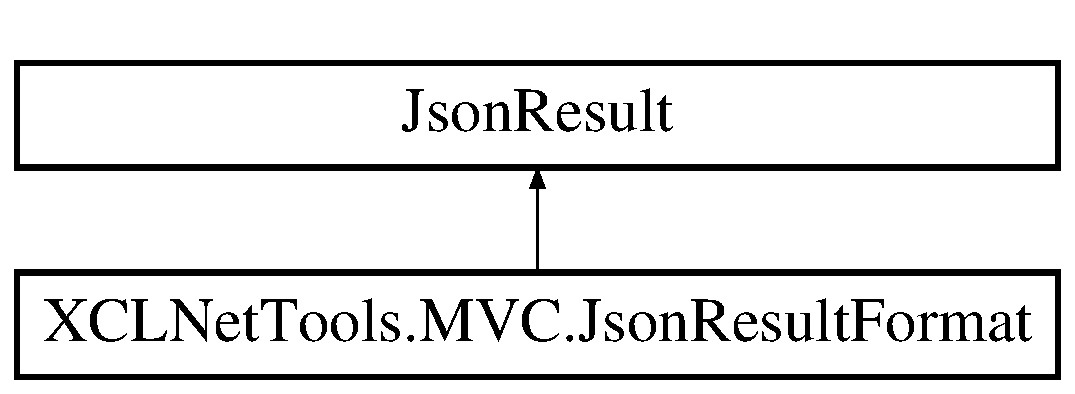
\includegraphics[height=2.000000cm]{class_x_c_l_net_tools_1_1_m_v_c_1_1_json_result_format}
\end{center}
\end{figure}
\subsection*{Public 成员函数}
\begin{DoxyCompactItemize}
\item 
override void \hyperlink{class_x_c_l_net_tools_1_1_m_v_c_1_1_json_result_format_aa8f3283c42c9130afd1aa8990876f413}{Execute\-Result} (Controller\-Context context)
\begin{DoxyCompactList}\small\item\em 重写执行视图 \end{DoxyCompactList}\end{DoxyCompactItemize}
\subsection*{属性}
\begin{DoxyCompactItemize}
\item 
string \hyperlink{class_x_c_l_net_tools_1_1_m_v_c_1_1_json_result_format_afc01b7cf2cd3f17c481c25ad70fcd4f6}{Date\-Format}\hspace{0.3cm}{\ttfamily  \mbox{[}get, set\mbox{]}}
\begin{DoxyCompactList}\small\item\em 格式化时间,默认值为\char`\"{}yyyy-\/\-M\-M-\/dd H\-H\-:mm\-:ss\char`\"{} \end{DoxyCompactList}\end{DoxyCompactItemize}


\subsection{详细描述}
带时间格式的json\-Result 



在文件 Json\-Result\-Format.\-cs 第 19 行定义.



\subsection{成员函数说明}
\hypertarget{class_x_c_l_net_tools_1_1_m_v_c_1_1_json_result_format_aa8f3283c42c9130afd1aa8990876f413}{\index{X\-C\-L\-Net\-Tools\-::\-M\-V\-C\-::\-Json\-Result\-Format@{X\-C\-L\-Net\-Tools\-::\-M\-V\-C\-::\-Json\-Result\-Format}!Execute\-Result@{Execute\-Result}}
\index{Execute\-Result@{Execute\-Result}!XCLNetTools::MVC::JsonResultFormat@{X\-C\-L\-Net\-Tools\-::\-M\-V\-C\-::\-Json\-Result\-Format}}
\subsubsection[{Execute\-Result}]{\setlength{\rightskip}{0pt plus 5cm}override void X\-C\-L\-Net\-Tools.\-M\-V\-C.\-Json\-Result\-Format.\-Execute\-Result (
\begin{DoxyParamCaption}
\item[{Controller\-Context}]{context}
\end{DoxyParamCaption}
)}}\label{class_x_c_l_net_tools_1_1_m_v_c_1_1_json_result_format_aa8f3283c42c9130afd1aa8990876f413}


重写执行视图 


\begin{DoxyParams}{参数}
{\em context} & 上下文\\
\hline
\end{DoxyParams}


在文件 Json\-Result\-Format.\-cs 第 36 行定义.



\subsection{属性说明}
\hypertarget{class_x_c_l_net_tools_1_1_m_v_c_1_1_json_result_format_afc01b7cf2cd3f17c481c25ad70fcd4f6}{\index{X\-C\-L\-Net\-Tools\-::\-M\-V\-C\-::\-Json\-Result\-Format@{X\-C\-L\-Net\-Tools\-::\-M\-V\-C\-::\-Json\-Result\-Format}!Date\-Format@{Date\-Format}}
\index{Date\-Format@{Date\-Format}!XCLNetTools::MVC::JsonResultFormat@{X\-C\-L\-Net\-Tools\-::\-M\-V\-C\-::\-Json\-Result\-Format}}
\subsubsection[{Date\-Format}]{\setlength{\rightskip}{0pt plus 5cm}string X\-C\-L\-Net\-Tools.\-M\-V\-C.\-Json\-Result\-Format.\-Date\-Format\hspace{0.3cm}{\ttfamily [get]}, {\ttfamily [set]}}}\label{class_x_c_l_net_tools_1_1_m_v_c_1_1_json_result_format_afc01b7cf2cd3f17c481c25ad70fcd4f6}


格式化时间,默认值为\char`\"{}yyyy-\/\-M\-M-\/dd H\-H\-:mm\-:ss\char`\"{} 



在文件 Json\-Result\-Format.\-cs 第 27 行定义.



该类的文档由以下文件生成\-:\begin{DoxyCompactItemize}
\item 
D\-:/\-My\-Data/\-My\-Git/\-Git\-Hub/\-X\-C\-L\-Net\-Tools/\-X\-C\-L\-Net\-Tools/\-M\-V\-C/\hyperlink{_json_result_format_8cs}{Json\-Result\-Format.\-cs}\end{DoxyCompactItemize}

\hypertarget{class_x_c_l_net_tools_1_1_entity_1_1_key_value}{}\section{X\+C\+L\+Net\+Tools.\+Entity.\+Key\+Value类 参考}
\label{class_x_c_l_net_tools_1_1_entity_1_1_key_value}\index{X\+C\+L\+Net\+Tools.\+Entity.\+Key\+Value@{X\+C\+L\+Net\+Tools.\+Entity.\+Key\+Value}}


键值类  


\subsection*{属性}
\begin{DoxyCompactItemize}
\item 
string \hyperlink{class_x_c_l_net_tools_1_1_entity_1_1_key_value_a33e2f7bfdcc6a1dce560304a4450cf08}{Key}\hspace{0.3cm}{\ttfamily  \mbox{[}get, set\mbox{]}}
\begin{DoxyCompactList}\small\item\em 键 \end{DoxyCompactList}\item 
string \hyperlink{class_x_c_l_net_tools_1_1_entity_1_1_key_value_a9ec3c76143930f64c1e0de2074514bae}{Value}\hspace{0.3cm}{\ttfamily  \mbox{[}get, set\mbox{]}}
\begin{DoxyCompactList}\small\item\em 值 \end{DoxyCompactList}\end{DoxyCompactItemize}


\subsection{详细描述}
键值类 



在文件 Key\+Value.\+cs 第 17 行定义.



\subsection{属性说明}
\mbox{\Hypertarget{class_x_c_l_net_tools_1_1_entity_1_1_key_value_a33e2f7bfdcc6a1dce560304a4450cf08}\label{class_x_c_l_net_tools_1_1_entity_1_1_key_value_a33e2f7bfdcc6a1dce560304a4450cf08}} 
\index{X\+C\+L\+Net\+Tools\+::\+Entity\+::\+Key\+Value@{X\+C\+L\+Net\+Tools\+::\+Entity\+::\+Key\+Value}!Key@{Key}}
\index{Key@{Key}!X\+C\+L\+Net\+Tools\+::\+Entity\+::\+Key\+Value@{X\+C\+L\+Net\+Tools\+::\+Entity\+::\+Key\+Value}}
\subsubsection{\texorpdfstring{Key}{Key}}
{\footnotesize\ttfamily string X\+C\+L\+Net\+Tools.\+Entity.\+Key\+Value.\+Key\hspace{0.3cm}{\ttfamily [get]}, {\ttfamily [set]}}



键 



在文件 Key\+Value.\+cs 第 22 行定义.

\mbox{\Hypertarget{class_x_c_l_net_tools_1_1_entity_1_1_key_value_a9ec3c76143930f64c1e0de2074514bae}\label{class_x_c_l_net_tools_1_1_entity_1_1_key_value_a9ec3c76143930f64c1e0de2074514bae}} 
\index{X\+C\+L\+Net\+Tools\+::\+Entity\+::\+Key\+Value@{X\+C\+L\+Net\+Tools\+::\+Entity\+::\+Key\+Value}!Value@{Value}}
\index{Value@{Value}!X\+C\+L\+Net\+Tools\+::\+Entity\+::\+Key\+Value@{X\+C\+L\+Net\+Tools\+::\+Entity\+::\+Key\+Value}}
\subsubsection{\texorpdfstring{Value}{Value}}
{\footnotesize\ttfamily string X\+C\+L\+Net\+Tools.\+Entity.\+Key\+Value.\+Value\hspace{0.3cm}{\ttfamily [get]}, {\ttfamily [set]}}



值 



在文件 Key\+Value.\+cs 第 27 行定义.



该类的文档由以下文件生成\+:\begin{DoxyCompactItemize}
\item 
D\+:/\+My\+Data/\+Git\+Hub/\+X\+C\+L\+Net\+Tools/\+X\+C\+L\+Net\+Tools/\+Entity/\hyperlink{_key_value_8cs}{Key\+Value.\+cs}\end{DoxyCompactItemize}

\hypertarget{class_x_c_l_net_tools_1_1_message_1_1_message_model}{}\section{X\+C\+L\+Net\+Tools.\+Message.\+Message\+Model类 参考}
\label{class_x_c_l_net_tools_1_1_message_1_1_message_model}\index{X\+C\+L\+Net\+Tools.\+Message.\+Message\+Model@{X\+C\+L\+Net\+Tools.\+Message.\+Message\+Model}}


消息提示实体类(用于json属性)  


\subsection*{属性}
\begin{DoxyCompactItemize}
\item 
virtual string \hyperlink{class_x_c_l_net_tools_1_1_message_1_1_message_model_a2347b5cf1ac7736de79aa94abd252d85}{Title}\hspace{0.3cm}{\ttfamily  \mbox{[}get, set\mbox{]}}
\begin{DoxyCompactList}\small\item\em 提示标题 \end{DoxyCompactList}\item 
virtual Date\+Time \hyperlink{class_x_c_l_net_tools_1_1_message_1_1_message_model_a04ede00490c3dbabea1fc01e6150715a}{Date}\hspace{0.3cm}{\ttfamily  \mbox{[}get, set\mbox{]}}
\begin{DoxyCompactList}\small\item\em 消息提示时间 \end{DoxyCompactList}\item 
virtual string \hyperlink{class_x_c_l_net_tools_1_1_message_1_1_message_model_a1fb1dde64c832e59d688d9a9fe944da5}{Message}\hspace{0.3cm}{\ttfamily  \mbox{[}get, set\mbox{]}}
\begin{DoxyCompactList}\small\item\em 消息提示内容 \end{DoxyCompactList}\item 
virtual string \hyperlink{class_x_c_l_net_tools_1_1_message_1_1_message_model_ae30c575345756a20443bb2f26ecdf1e9}{Message\+More}\hspace{0.3cm}{\ttfamily  \mbox{[}get, set\mbox{]}}
\begin{DoxyCompactList}\small\item\em 消息详细信息 \end{DoxyCompactList}\item 
virtual string \hyperlink{class_x_c_l_net_tools_1_1_message_1_1_message_model_a35cd14fdd9bbc8dea4c151c00d538755}{Url}\hspace{0.3cm}{\ttfamily  \mbox{[}get, set\mbox{]}}
\begin{DoxyCompactList}\small\item\em 消息发生页地址 \end{DoxyCompactList}\item 
virtual string \hyperlink{class_x_c_l_net_tools_1_1_message_1_1_message_model_a36e0a2784c189c86b33b76ceca539a28}{From\+Url}\hspace{0.3cm}{\ttfamily  \mbox{[}get, set\mbox{]}}
\begin{DoxyCompactList}\small\item\em 消息页来源地址(reffer) \end{DoxyCompactList}\item 
virtual bool \hyperlink{class_x_c_l_net_tools_1_1_message_1_1_message_model_a3881fb689ec30bfd21672b010a130675}{Is\+Success}\hspace{0.3cm}{\ttfamily  \mbox{[}get, set\mbox{]}}
\begin{DoxyCompactList}\small\item\em 是否成功与失败的标识 \end{DoxyCompactList}\item 
virtual bool \hyperlink{class_x_c_l_net_tools_1_1_message_1_1_message_model_a07c51819ac5836a7839b778c2cc62ba5}{Is\+Refresh}\hspace{0.3cm}{\ttfamily  \mbox{[}get, set\mbox{]}}
\begin{DoxyCompactList}\small\item\em 是否需要刷新 \end{DoxyCompactList}\item 
virtual string \hyperlink{class_x_c_l_net_tools_1_1_message_1_1_message_model_a933d98b3a93f2aefeaaf2d66940133a9}{Remark}\hspace{0.3cm}{\ttfamily  \mbox{[}get, set\mbox{]}}
\begin{DoxyCompactList}\small\item\em 备注信息 \end{DoxyCompactList}\item 
virtual bool \hyperlink{class_x_c_l_net_tools_1_1_message_1_1_message_model_af7a1590f9d2745c3db1486cb39edc070}{Is\+Redirect}\hspace{0.3cm}{\ttfamily  \mbox{[}get, set\mbox{]}}
\begin{DoxyCompactList}\small\item\em 是否需要跳转 \end{DoxyCompactList}\item 
virtual string \hyperlink{class_x_c_l_net_tools_1_1_message_1_1_message_model_a571c6e0204605733f900eb3f906e038d}{Redirect\+U\+RL}\hspace{0.3cm}{\ttfamily  \mbox{[}get, set\mbox{]}}
\begin{DoxyCompactList}\small\item\em 要跳转的url \end{DoxyCompactList}\item 
virtual \hyperlink{class_x_c_l_net_tools_1_1_enum_1_1_common_enum_a1cd31513e5ecf78c77d76be7954ae2f4}{X\+C\+L\+Net\+Tools.\+Enum.\+Common\+Enum.\+Redirect\+Target\+Enum} \hyperlink{class_x_c_l_net_tools_1_1_message_1_1_message_model_a318553f7c9db2b2c685e4944feb2901e}{Redirect\+Target}\hspace{0.3cm}{\ttfamily  \mbox{[}get, set\mbox{]}}
\begin{DoxyCompactList}\small\item\em 跳转方式 \end{DoxyCompactList}\item 
virtual bool \hyperlink{class_x_c_l_net_tools_1_1_message_1_1_message_model_a1ea24cc20f05516f6266af92cc06479a}{Is\+Ajax}\hspace{0.3cm}{\ttfamily  \mbox{[}get\mbox{]}}
\begin{DoxyCompactList}\small\item\em 当前请求是否为ajax请求 \end{DoxyCompactList}\item 
virtual string \hyperlink{class_x_c_l_net_tools_1_1_message_1_1_message_model_ab169d7bab20868e935d775459b72e625}{Error\+Code}\hspace{0.3cm}{\ttfamily  \mbox{[}get, set\mbox{]}}
\begin{DoxyCompactList}\small\item\em 错误码 \end{DoxyCompactList}\item 
virtual object \hyperlink{class_x_c_l_net_tools_1_1_message_1_1_message_model_a8065226d89965a09b9ff8e69ba9974ca}{Custom\+Object}\hspace{0.3cm}{\ttfamily  \mbox{[}get, set\mbox{]}}
\begin{DoxyCompactList}\small\item\em 自定义输出对象 \end{DoxyCompactList}\end{DoxyCompactItemize}


\subsection{详细描述}
消息提示实体类(用于json属性) 



在文件 Message\+Model.\+cs 第 19 行定义.



\subsection{属性说明}
\index{X\+C\+L\+Net\+Tools\+::\+Message\+::\+Message\+Model@{X\+C\+L\+Net\+Tools\+::\+Message\+::\+Message\+Model}!Custom\+Object@{Custom\+Object}}
\index{Custom\+Object@{Custom\+Object}!X\+C\+L\+Net\+Tools\+::\+Message\+::\+Message\+Model@{X\+C\+L\+Net\+Tools\+::\+Message\+::\+Message\+Model}}
\subsubsection[{\texorpdfstring{Custom\+Object}{CustomObject}}]{\setlength{\rightskip}{0pt plus 5cm}virtual object X\+C\+L\+Net\+Tools.\+Message.\+Message\+Model.\+Custom\+Object\hspace{0.3cm}{\ttfamily [get]}, {\ttfamily [set]}}\hypertarget{class_x_c_l_net_tools_1_1_message_1_1_message_model_a8065226d89965a09b9ff8e69ba9974ca}{}\label{class_x_c_l_net_tools_1_1_message_1_1_message_model_a8065226d89965a09b9ff8e69ba9974ca}


自定义输出对象 



在文件 Message\+Model.\+cs 第 115 行定义.

\index{X\+C\+L\+Net\+Tools\+::\+Message\+::\+Message\+Model@{X\+C\+L\+Net\+Tools\+::\+Message\+::\+Message\+Model}!Date@{Date}}
\index{Date@{Date}!X\+C\+L\+Net\+Tools\+::\+Message\+::\+Message\+Model@{X\+C\+L\+Net\+Tools\+::\+Message\+::\+Message\+Model}}
\subsubsection[{\texorpdfstring{Date}{Date}}]{\setlength{\rightskip}{0pt plus 5cm}virtual Date\+Time X\+C\+L\+Net\+Tools.\+Message.\+Message\+Model.\+Date\hspace{0.3cm}{\ttfamily [get]}, {\ttfamily [set]}}\hypertarget{class_x_c_l_net_tools_1_1_message_1_1_message_model_a04ede00490c3dbabea1fc01e6150715a}{}\label{class_x_c_l_net_tools_1_1_message_1_1_message_model_a04ede00490c3dbabea1fc01e6150715a}


消息提示时间 



在文件 Message\+Model.\+cs 第 31 行定义.

\index{X\+C\+L\+Net\+Tools\+::\+Message\+::\+Message\+Model@{X\+C\+L\+Net\+Tools\+::\+Message\+::\+Message\+Model}!Error\+Code@{Error\+Code}}
\index{Error\+Code@{Error\+Code}!X\+C\+L\+Net\+Tools\+::\+Message\+::\+Message\+Model@{X\+C\+L\+Net\+Tools\+::\+Message\+::\+Message\+Model}}
\subsubsection[{\texorpdfstring{Error\+Code}{ErrorCode}}]{\setlength{\rightskip}{0pt plus 5cm}virtual string X\+C\+L\+Net\+Tools.\+Message.\+Message\+Model.\+Error\+Code\hspace{0.3cm}{\ttfamily [get]}, {\ttfamily [set]}}\hypertarget{class_x_c_l_net_tools_1_1_message_1_1_message_model_ab169d7bab20868e935d775459b72e625}{}\label{class_x_c_l_net_tools_1_1_message_1_1_message_model_ab169d7bab20868e935d775459b72e625}


错误码 



在文件 Message\+Model.\+cs 第 109 行定义.

\index{X\+C\+L\+Net\+Tools\+::\+Message\+::\+Message\+Model@{X\+C\+L\+Net\+Tools\+::\+Message\+::\+Message\+Model}!From\+Url@{From\+Url}}
\index{From\+Url@{From\+Url}!X\+C\+L\+Net\+Tools\+::\+Message\+::\+Message\+Model@{X\+C\+L\+Net\+Tools\+::\+Message\+::\+Message\+Model}}
\subsubsection[{\texorpdfstring{From\+Url}{FromUrl}}]{\setlength{\rightskip}{0pt plus 5cm}virtual string X\+C\+L\+Net\+Tools.\+Message.\+Message\+Model.\+From\+Url\hspace{0.3cm}{\ttfamily [get]}, {\ttfamily [set]}}\hypertarget{class_x_c_l_net_tools_1_1_message_1_1_message_model_a36e0a2784c189c86b33b76ceca539a28}{}\label{class_x_c_l_net_tools_1_1_message_1_1_message_model_a36e0a2784c189c86b33b76ceca539a28}


消息页来源地址(reffer) 



在文件 Message\+Model.\+cs 第 55 行定义.

\index{X\+C\+L\+Net\+Tools\+::\+Message\+::\+Message\+Model@{X\+C\+L\+Net\+Tools\+::\+Message\+::\+Message\+Model}!Is\+Ajax@{Is\+Ajax}}
\index{Is\+Ajax@{Is\+Ajax}!X\+C\+L\+Net\+Tools\+::\+Message\+::\+Message\+Model@{X\+C\+L\+Net\+Tools\+::\+Message\+::\+Message\+Model}}
\subsubsection[{\texorpdfstring{Is\+Ajax}{IsAjax}}]{\setlength{\rightskip}{0pt plus 5cm}virtual bool X\+C\+L\+Net\+Tools.\+Message.\+Message\+Model.\+Is\+Ajax\hspace{0.3cm}{\ttfamily [get]}}\hypertarget{class_x_c_l_net_tools_1_1_message_1_1_message_model_a1ea24cc20f05516f6266af92cc06479a}{}\label{class_x_c_l_net_tools_1_1_message_1_1_message_model_a1ea24cc20f05516f6266af92cc06479a}


当前请求是否为ajax请求 



在文件 Message\+Model.\+cs 第 98 行定义.

\index{X\+C\+L\+Net\+Tools\+::\+Message\+::\+Message\+Model@{X\+C\+L\+Net\+Tools\+::\+Message\+::\+Message\+Model}!Is\+Redirect@{Is\+Redirect}}
\index{Is\+Redirect@{Is\+Redirect}!X\+C\+L\+Net\+Tools\+::\+Message\+::\+Message\+Model@{X\+C\+L\+Net\+Tools\+::\+Message\+::\+Message\+Model}}
\subsubsection[{\texorpdfstring{Is\+Redirect}{IsRedirect}}]{\setlength{\rightskip}{0pt plus 5cm}virtual bool X\+C\+L\+Net\+Tools.\+Message.\+Message\+Model.\+Is\+Redirect\hspace{0.3cm}{\ttfamily [get]}, {\ttfamily [set]}}\hypertarget{class_x_c_l_net_tools_1_1_message_1_1_message_model_af7a1590f9d2745c3db1486cb39edc070}{}\label{class_x_c_l_net_tools_1_1_message_1_1_message_model_af7a1590f9d2745c3db1486cb39edc070}


是否需要跳转 



在文件 Message\+Model.\+cs 第 79 行定义.

\index{X\+C\+L\+Net\+Tools\+::\+Message\+::\+Message\+Model@{X\+C\+L\+Net\+Tools\+::\+Message\+::\+Message\+Model}!Is\+Refresh@{Is\+Refresh}}
\index{Is\+Refresh@{Is\+Refresh}!X\+C\+L\+Net\+Tools\+::\+Message\+::\+Message\+Model@{X\+C\+L\+Net\+Tools\+::\+Message\+::\+Message\+Model}}
\subsubsection[{\texorpdfstring{Is\+Refresh}{IsRefresh}}]{\setlength{\rightskip}{0pt plus 5cm}virtual bool X\+C\+L\+Net\+Tools.\+Message.\+Message\+Model.\+Is\+Refresh\hspace{0.3cm}{\ttfamily [get]}, {\ttfamily [set]}}\hypertarget{class_x_c_l_net_tools_1_1_message_1_1_message_model_a07c51819ac5836a7839b778c2cc62ba5}{}\label{class_x_c_l_net_tools_1_1_message_1_1_message_model_a07c51819ac5836a7839b778c2cc62ba5}


是否需要刷新 



在文件 Message\+Model.\+cs 第 67 行定义.

\index{X\+C\+L\+Net\+Tools\+::\+Message\+::\+Message\+Model@{X\+C\+L\+Net\+Tools\+::\+Message\+::\+Message\+Model}!Is\+Success@{Is\+Success}}
\index{Is\+Success@{Is\+Success}!X\+C\+L\+Net\+Tools\+::\+Message\+::\+Message\+Model@{X\+C\+L\+Net\+Tools\+::\+Message\+::\+Message\+Model}}
\subsubsection[{\texorpdfstring{Is\+Success}{IsSuccess}}]{\setlength{\rightskip}{0pt plus 5cm}virtual bool X\+C\+L\+Net\+Tools.\+Message.\+Message\+Model.\+Is\+Success\hspace{0.3cm}{\ttfamily [get]}, {\ttfamily [set]}}\hypertarget{class_x_c_l_net_tools_1_1_message_1_1_message_model_a3881fb689ec30bfd21672b010a130675}{}\label{class_x_c_l_net_tools_1_1_message_1_1_message_model_a3881fb689ec30bfd21672b010a130675}


是否成功与失败的标识 



在文件 Message\+Model.\+cs 第 61 行定义.

\index{X\+C\+L\+Net\+Tools\+::\+Message\+::\+Message\+Model@{X\+C\+L\+Net\+Tools\+::\+Message\+::\+Message\+Model}!Message@{Message}}
\index{Message@{Message}!X\+C\+L\+Net\+Tools\+::\+Message\+::\+Message\+Model@{X\+C\+L\+Net\+Tools\+::\+Message\+::\+Message\+Model}}
\subsubsection[{\texorpdfstring{Message}{Message}}]{\setlength{\rightskip}{0pt plus 5cm}virtual string X\+C\+L\+Net\+Tools.\+Message.\+Message\+Model.\+Message\hspace{0.3cm}{\ttfamily [get]}, {\ttfamily [set]}}\hypertarget{class_x_c_l_net_tools_1_1_message_1_1_message_model_a1fb1dde64c832e59d688d9a9fe944da5}{}\label{class_x_c_l_net_tools_1_1_message_1_1_message_model_a1fb1dde64c832e59d688d9a9fe944da5}


消息提示内容 



在文件 Message\+Model.\+cs 第 37 行定义.

\index{X\+C\+L\+Net\+Tools\+::\+Message\+::\+Message\+Model@{X\+C\+L\+Net\+Tools\+::\+Message\+::\+Message\+Model}!Message\+More@{Message\+More}}
\index{Message\+More@{Message\+More}!X\+C\+L\+Net\+Tools\+::\+Message\+::\+Message\+Model@{X\+C\+L\+Net\+Tools\+::\+Message\+::\+Message\+Model}}
\subsubsection[{\texorpdfstring{Message\+More}{MessageMore}}]{\setlength{\rightskip}{0pt plus 5cm}virtual string X\+C\+L\+Net\+Tools.\+Message.\+Message\+Model.\+Message\+More\hspace{0.3cm}{\ttfamily [get]}, {\ttfamily [set]}}\hypertarget{class_x_c_l_net_tools_1_1_message_1_1_message_model_ae30c575345756a20443bb2f26ecdf1e9}{}\label{class_x_c_l_net_tools_1_1_message_1_1_message_model_ae30c575345756a20443bb2f26ecdf1e9}


消息详细信息 



在文件 Message\+Model.\+cs 第 43 行定义.

\index{X\+C\+L\+Net\+Tools\+::\+Message\+::\+Message\+Model@{X\+C\+L\+Net\+Tools\+::\+Message\+::\+Message\+Model}!Redirect\+Target@{Redirect\+Target}}
\index{Redirect\+Target@{Redirect\+Target}!X\+C\+L\+Net\+Tools\+::\+Message\+::\+Message\+Model@{X\+C\+L\+Net\+Tools\+::\+Message\+::\+Message\+Model}}
\subsubsection[{\texorpdfstring{Redirect\+Target}{RedirectTarget}}]{\setlength{\rightskip}{0pt plus 5cm}virtual {\bf X\+C\+L\+Net\+Tools.\+Enum.\+Common\+Enum.\+Redirect\+Target\+Enum} X\+C\+L\+Net\+Tools.\+Message.\+Message\+Model.\+Redirect\+Target\hspace{0.3cm}{\ttfamily [get]}, {\ttfamily [set]}}\hypertarget{class_x_c_l_net_tools_1_1_message_1_1_message_model_a318553f7c9db2b2c685e4944feb2901e}{}\label{class_x_c_l_net_tools_1_1_message_1_1_message_model_a318553f7c9db2b2c685e4944feb2901e}


跳转方式 



在文件 Message\+Model.\+cs 第 91 行定义.

\index{X\+C\+L\+Net\+Tools\+::\+Message\+::\+Message\+Model@{X\+C\+L\+Net\+Tools\+::\+Message\+::\+Message\+Model}!Redirect\+U\+RL@{Redirect\+U\+RL}}
\index{Redirect\+U\+RL@{Redirect\+U\+RL}!X\+C\+L\+Net\+Tools\+::\+Message\+::\+Message\+Model@{X\+C\+L\+Net\+Tools\+::\+Message\+::\+Message\+Model}}
\subsubsection[{\texorpdfstring{Redirect\+U\+RL}{RedirectURL}}]{\setlength{\rightskip}{0pt plus 5cm}virtual string X\+C\+L\+Net\+Tools.\+Message.\+Message\+Model.\+Redirect\+U\+RL\hspace{0.3cm}{\ttfamily [get]}, {\ttfamily [set]}}\hypertarget{class_x_c_l_net_tools_1_1_message_1_1_message_model_a571c6e0204605733f900eb3f906e038d}{}\label{class_x_c_l_net_tools_1_1_message_1_1_message_model_a571c6e0204605733f900eb3f906e038d}


要跳转的url 



在文件 Message\+Model.\+cs 第 85 行定义.

\index{X\+C\+L\+Net\+Tools\+::\+Message\+::\+Message\+Model@{X\+C\+L\+Net\+Tools\+::\+Message\+::\+Message\+Model}!Remark@{Remark}}
\index{Remark@{Remark}!X\+C\+L\+Net\+Tools\+::\+Message\+::\+Message\+Model@{X\+C\+L\+Net\+Tools\+::\+Message\+::\+Message\+Model}}
\subsubsection[{\texorpdfstring{Remark}{Remark}}]{\setlength{\rightskip}{0pt plus 5cm}virtual string X\+C\+L\+Net\+Tools.\+Message.\+Message\+Model.\+Remark\hspace{0.3cm}{\ttfamily [get]}, {\ttfamily [set]}}\hypertarget{class_x_c_l_net_tools_1_1_message_1_1_message_model_a933d98b3a93f2aefeaaf2d66940133a9}{}\label{class_x_c_l_net_tools_1_1_message_1_1_message_model_a933d98b3a93f2aefeaaf2d66940133a9}


备注信息 



在文件 Message\+Model.\+cs 第 73 行定义.

\index{X\+C\+L\+Net\+Tools\+::\+Message\+::\+Message\+Model@{X\+C\+L\+Net\+Tools\+::\+Message\+::\+Message\+Model}!Title@{Title}}
\index{Title@{Title}!X\+C\+L\+Net\+Tools\+::\+Message\+::\+Message\+Model@{X\+C\+L\+Net\+Tools\+::\+Message\+::\+Message\+Model}}
\subsubsection[{\texorpdfstring{Title}{Title}}]{\setlength{\rightskip}{0pt plus 5cm}virtual string X\+C\+L\+Net\+Tools.\+Message.\+Message\+Model.\+Title\hspace{0.3cm}{\ttfamily [get]}, {\ttfamily [set]}}\hypertarget{class_x_c_l_net_tools_1_1_message_1_1_message_model_a2347b5cf1ac7736de79aa94abd252d85}{}\label{class_x_c_l_net_tools_1_1_message_1_1_message_model_a2347b5cf1ac7736de79aa94abd252d85}


提示标题 



在文件 Message\+Model.\+cs 第 25 行定义.

\index{X\+C\+L\+Net\+Tools\+::\+Message\+::\+Message\+Model@{X\+C\+L\+Net\+Tools\+::\+Message\+::\+Message\+Model}!Url@{Url}}
\index{Url@{Url}!X\+C\+L\+Net\+Tools\+::\+Message\+::\+Message\+Model@{X\+C\+L\+Net\+Tools\+::\+Message\+::\+Message\+Model}}
\subsubsection[{\texorpdfstring{Url}{Url}}]{\setlength{\rightskip}{0pt plus 5cm}virtual string X\+C\+L\+Net\+Tools.\+Message.\+Message\+Model.\+Url\hspace{0.3cm}{\ttfamily [get]}, {\ttfamily [set]}}\hypertarget{class_x_c_l_net_tools_1_1_message_1_1_message_model_a35cd14fdd9bbc8dea4c151c00d538755}{}\label{class_x_c_l_net_tools_1_1_message_1_1_message_model_a35cd14fdd9bbc8dea4c151c00d538755}


消息发生页地址 



在文件 Message\+Model.\+cs 第 49 行定义.



该类的文档由以下文件生成\+:\begin{DoxyCompactItemize}
\item 
E\+:/\+Git\+Hub/\+X\+C\+L\+Net\+Tools/\+X\+C\+L\+Net\+Tools/\+Message/\hyperlink{_message_model_8cs}{Message\+Model.\+cs}\end{DoxyCompactItemize}

\hypertarget{class_x_c_l_net_tools_1_1_entity_1_1_method_result}{}\section{X\+C\+L\+Net\+Tools.\+Entity.\+Method\+Result$<$ T\+Result $>$ 模板类 参考}
\label{class_x_c_l_net_tools_1_1_entity_1_1_method_result}\index{X\+C\+L\+Net\+Tools.\+Entity.\+Method\+Result$<$ T\+Result $>$@{X\+C\+L\+Net\+Tools.\+Entity.\+Method\+Result$<$ T\+Result $>$}}


方法返回值实体,主要是方便一个方法输出多个信息时使用,同时也减少使用out返回结果信息  




\subsection{详细描述}
方法返回值实体,主要是方便一个方法输出多个信息时使用,同时也减少使用out返回结果信息 


\begin{DoxyTemplParams}{Template Parameters}
{\em T\+Result} & 方法返回的结果类型\\
\hline
\end{DoxyTemplParams}


在文件 Method\+Result.\+cs 第 18 行定义.



该类的文档由以下文件生成\+:\begin{DoxyCompactItemize}
\item 
E\+:/\+Git\+Hub/\+X\+C\+L\+Net\+Tools/\+X\+C\+L\+Net\+Tools/\+Entity/\hyperlink{_method_result_8cs}{Method\+Result.\+cs}\end{DoxyCompactItemize}

\hypertarget{class_x_c_l_net_tools_1_1_entity_1_1_method_result}{}\section{X\+C\+L\+Net\+Tools.\+Entity.\+Method\+Result$<$ T\+Result $>$ 模板类 参考}
\label{class_x_c_l_net_tools_1_1_entity_1_1_method_result}\index{X\+C\+L\+Net\+Tools.\+Entity.\+Method\+Result$<$ T\+Result $>$@{X\+C\+L\+Net\+Tools.\+Entity.\+Method\+Result$<$ T\+Result $>$}}


方法返回值实体,主要是方便一个方法输出多个信息时使用,同时也减少使用out返回结果信息  




\subsection{详细描述}
方法返回值实体,主要是方便一个方法输出多个信息时使用,同时也减少使用out返回结果信息 


\begin{DoxyTemplParams}{Template Parameters}
{\em T\+Result} & 方法返回的结果类型\\
\hline
\end{DoxyTemplParams}


在文件 Method\+Result.\+cs 第 18 行定义.



该类的文档由以下文件生成\+:\begin{DoxyCompactItemize}
\item 
E\+:/\+Git\+Hub/\+X\+C\+L\+Net\+Tools/\+X\+C\+L\+Net\+Tools/\+Entity/\hyperlink{_method_result_8cs}{Method\+Result.\+cs}\end{DoxyCompactItemize}

\hypertarget{class_x_c_l_net_tools_1_1_file_handler_1_1_multipart_form}{\section{X\-C\-L\-Net\-Tools.\-File\-Handler.\-Multipart\-Form类 参考}
\label{class_x_c_l_net_tools_1_1_file_handler_1_1_multipart_form}\index{X\-C\-L\-Net\-Tools.\-File\-Handler.\-Multipart\-Form@{X\-C\-L\-Net\-Tools.\-File\-Handler.\-Multipart\-Form}}
}


对文件和文本数据进行\-Multipart形式的编码  


\subsection*{Public 成员函数}
\begin{DoxyCompactItemize}
\item 
\hyperlink{class_x_c_l_net_tools_1_1_file_handler_1_1_multipart_form_ab1d1debcf1e0f5dc05e9758f72b4500d}{Multipart\-Form} ()
\begin{DoxyCompactList}\small\item\em 实例化 \end{DoxyCompactList}\item 
void \hyperlink{class_x_c_l_net_tools_1_1_file_handler_1_1_multipart_form_af2601517bb4cafc5c9648945ed3e5572}{Add\-Flie} (string name, string filename)
\begin{DoxyCompactList}\small\item\em 添加一个文件 \end{DoxyCompactList}\item 
void \hyperlink{class_x_c_l_net_tools_1_1_file_handler_1_1_multipart_form_a5b531d40e9baf9f5ca51260bd4403b00}{Add\-Flie} (string name, string filename, byte\mbox{[}$\,$\mbox{]} file\-Data, int data\-Length)
\begin{DoxyCompactList}\small\item\em 添加一个文件 \end{DoxyCompactList}\item 
void \hyperlink{class_x_c_l_net_tools_1_1_file_handler_1_1_multipart_form_ab791aa6797ff7253f448fbad17ec0841}{Add\-String} (string name, string value)
\begin{DoxyCompactList}\small\item\em 添加字符串 \end{DoxyCompactList}\end{DoxyCompactItemize}
\subsection*{属性}
\begin{DoxyCompactItemize}
\item 
byte\mbox{[}$\,$\mbox{]} \hyperlink{class_x_c_l_net_tools_1_1_file_handler_1_1_multipart_form_ad540886372239dbb4fcc975e694be5d9}{Form\-Data}\hspace{0.3cm}{\ttfamily  \mbox{[}get\mbox{]}}
\begin{DoxyCompactList}\small\item\em 获取编码后的字节数组 \end{DoxyCompactList}\item 
string \hyperlink{class_x_c_l_net_tools_1_1_file_handler_1_1_multipart_form_a634f22e875a4d7eb49a729dcb2903f86}{Content\-Type}\hspace{0.3cm}{\ttfamily  \mbox{[}get\mbox{]}}
\begin{DoxyCompactList}\small\item\em 获取此编码内容的类型 \end{DoxyCompactList}\item 
Encoding \hyperlink{class_x_c_l_net_tools_1_1_file_handler_1_1_multipart_form_ade83206c0e41ad24ba543ebd89e0281f}{String\-Encoding}\hspace{0.3cm}{\ttfamily  \mbox{[}get, set\mbox{]}}
\begin{DoxyCompactList}\small\item\em 获取或设置对字符串采用的编码类型 \end{DoxyCompactList}\end{DoxyCompactItemize}


\subsection{详细描述}
对文件和文本数据进行\-Multipart形式的编码 



在文件 Http\-Proc.\-cs 第 443 行定义.



\subsection{构造及析构函数说明}
\hypertarget{class_x_c_l_net_tools_1_1_file_handler_1_1_multipart_form_ab1d1debcf1e0f5dc05e9758f72b4500d}{\index{X\-C\-L\-Net\-Tools\-::\-File\-Handler\-::\-Multipart\-Form@{X\-C\-L\-Net\-Tools\-::\-File\-Handler\-::\-Multipart\-Form}!Multipart\-Form@{Multipart\-Form}}
\index{Multipart\-Form@{Multipart\-Form}!XCLNetTools::FileHandler::MultipartForm@{X\-C\-L\-Net\-Tools\-::\-File\-Handler\-::\-Multipart\-Form}}
\subsubsection[{Multipart\-Form}]{\setlength{\rightskip}{0pt plus 5cm}X\-C\-L\-Net\-Tools.\-File\-Handler.\-Multipart\-Form.\-Multipart\-Form (
\begin{DoxyParamCaption}
{}
\end{DoxyParamCaption}
)}}\label{class_x_c_l_net_tools_1_1_file_handler_1_1_multipart_form_ab1d1debcf1e0f5dc05e9758f72b4500d}


实例化 



在文件 Http\-Proc.\-cs 第 487 行定义.



\subsection{成员函数说明}
\hypertarget{class_x_c_l_net_tools_1_1_file_handler_1_1_multipart_form_af2601517bb4cafc5c9648945ed3e5572}{\index{X\-C\-L\-Net\-Tools\-::\-File\-Handler\-::\-Multipart\-Form@{X\-C\-L\-Net\-Tools\-::\-File\-Handler\-::\-Multipart\-Form}!Add\-Flie@{Add\-Flie}}
\index{Add\-Flie@{Add\-Flie}!XCLNetTools::FileHandler::MultipartForm@{X\-C\-L\-Net\-Tools\-::\-File\-Handler\-::\-Multipart\-Form}}
\subsubsection[{Add\-Flie}]{\setlength{\rightskip}{0pt plus 5cm}void X\-C\-L\-Net\-Tools.\-File\-Handler.\-Multipart\-Form.\-Add\-Flie (
\begin{DoxyParamCaption}
\item[{string}]{name, }
\item[{string}]{filename}
\end{DoxyParamCaption}
)}}\label{class_x_c_l_net_tools_1_1_file_handler_1_1_multipart_form_af2601517bb4cafc5c9648945ed3e5572}


添加一个文件 


\begin{DoxyParams}{参数}
{\em name} & 文件域名称\\
\hline
{\em filename} & 文件的完整路径\\
\hline
\end{DoxyParams}


在文件 Http\-Proc.\-cs 第 499 行定义.

\hypertarget{class_x_c_l_net_tools_1_1_file_handler_1_1_multipart_form_a5b531d40e9baf9f5ca51260bd4403b00}{\index{X\-C\-L\-Net\-Tools\-::\-File\-Handler\-::\-Multipart\-Form@{X\-C\-L\-Net\-Tools\-::\-File\-Handler\-::\-Multipart\-Form}!Add\-Flie@{Add\-Flie}}
\index{Add\-Flie@{Add\-Flie}!XCLNetTools::FileHandler::MultipartForm@{X\-C\-L\-Net\-Tools\-::\-File\-Handler\-::\-Multipart\-Form}}
\subsubsection[{Add\-Flie}]{\setlength{\rightskip}{0pt plus 5cm}void X\-C\-L\-Net\-Tools.\-File\-Handler.\-Multipart\-Form.\-Add\-Flie (
\begin{DoxyParamCaption}
\item[{string}]{name, }
\item[{string}]{filename, }
\item[{byte\mbox{[}$\,$\mbox{]}}]{file\-Data, }
\item[{int}]{data\-Length}
\end{DoxyParamCaption}
)}}\label{class_x_c_l_net_tools_1_1_file_handler_1_1_multipart_form_a5b531d40e9baf9f5ca51260bd4403b00}


添加一个文件 


\begin{DoxyParams}{参数}
{\em name} & 文件域名称\\
\hline
{\em filename} & 文件名\\
\hline
{\em file\-Data} & 文件二进制数据\\
\hline
{\em data\-Length} & 二进制数据大小\\
\hline
\end{DoxyParams}


在文件 Http\-Proc.\-cs 第 529 行定义.

\hypertarget{class_x_c_l_net_tools_1_1_file_handler_1_1_multipart_form_ab791aa6797ff7253f448fbad17ec0841}{\index{X\-C\-L\-Net\-Tools\-::\-File\-Handler\-::\-Multipart\-Form@{X\-C\-L\-Net\-Tools\-::\-File\-Handler\-::\-Multipart\-Form}!Add\-String@{Add\-String}}
\index{Add\-String@{Add\-String}!XCLNetTools::FileHandler::MultipartForm@{X\-C\-L\-Net\-Tools\-::\-File\-Handler\-::\-Multipart\-Form}}
\subsubsection[{Add\-String}]{\setlength{\rightskip}{0pt plus 5cm}void X\-C\-L\-Net\-Tools.\-File\-Handler.\-Multipart\-Form.\-Add\-String (
\begin{DoxyParamCaption}
\item[{string}]{name, }
\item[{string}]{value}
\end{DoxyParamCaption}
)}}\label{class_x_c_l_net_tools_1_1_file_handler_1_1_multipart_form_ab791aa6797ff7253f448fbad17ec0841}


添加字符串 


\begin{DoxyParams}{参数}
{\em name} & 文本域名称\\
\hline
{\em value} & 文本值\\
\hline
\end{DoxyParams}


在文件 Http\-Proc.\-cs 第 552 行定义.



\subsection{属性说明}
\hypertarget{class_x_c_l_net_tools_1_1_file_handler_1_1_multipart_form_a634f22e875a4d7eb49a729dcb2903f86}{\index{X\-C\-L\-Net\-Tools\-::\-File\-Handler\-::\-Multipart\-Form@{X\-C\-L\-Net\-Tools\-::\-File\-Handler\-::\-Multipart\-Form}!Content\-Type@{Content\-Type}}
\index{Content\-Type@{Content\-Type}!XCLNetTools::FileHandler::MultipartForm@{X\-C\-L\-Net\-Tools\-::\-File\-Handler\-::\-Multipart\-Form}}
\subsubsection[{Content\-Type}]{\setlength{\rightskip}{0pt plus 5cm}string X\-C\-L\-Net\-Tools.\-File\-Handler.\-Multipart\-Form.\-Content\-Type\hspace{0.3cm}{\ttfamily [get]}}}\label{class_x_c_l_net_tools_1_1_file_handler_1_1_multipart_form_a634f22e875a4d7eb49a729dcb2903f86}


获取此编码内容的类型 



在文件 Http\-Proc.\-cs 第 471 行定义.

\hypertarget{class_x_c_l_net_tools_1_1_file_handler_1_1_multipart_form_ad540886372239dbb4fcc975e694be5d9}{\index{X\-C\-L\-Net\-Tools\-::\-File\-Handler\-::\-Multipart\-Form@{X\-C\-L\-Net\-Tools\-::\-File\-Handler\-::\-Multipart\-Form}!Form\-Data@{Form\-Data}}
\index{Form\-Data@{Form\-Data}!XCLNetTools::FileHandler::MultipartForm@{X\-C\-L\-Net\-Tools\-::\-File\-Handler\-::\-Multipart\-Form}}
\subsubsection[{Form\-Data}]{\setlength{\rightskip}{0pt plus 5cm}byte \mbox{[}$\,$\mbox{]} X\-C\-L\-Net\-Tools.\-File\-Handler.\-Multipart\-Form.\-Form\-Data\hspace{0.3cm}{\ttfamily [get]}}}\label{class_x_c_l_net_tools_1_1_file_handler_1_1_multipart_form_ad540886372239dbb4fcc975e694be5d9}


获取编码后的字节数组 



在文件 Http\-Proc.\-cs 第 454 行定义.

\hypertarget{class_x_c_l_net_tools_1_1_file_handler_1_1_multipart_form_ade83206c0e41ad24ba543ebd89e0281f}{\index{X\-C\-L\-Net\-Tools\-::\-File\-Handler\-::\-Multipart\-Form@{X\-C\-L\-Net\-Tools\-::\-File\-Handler\-::\-Multipart\-Form}!String\-Encoding@{String\-Encoding}}
\index{String\-Encoding@{String\-Encoding}!XCLNetTools::FileHandler::MultipartForm@{X\-C\-L\-Net\-Tools\-::\-File\-Handler\-::\-Multipart\-Form}}
\subsubsection[{String\-Encoding}]{\setlength{\rightskip}{0pt plus 5cm}Encoding X\-C\-L\-Net\-Tools.\-File\-Handler.\-Multipart\-Form.\-String\-Encoding\hspace{0.3cm}{\ttfamily [get]}, {\ttfamily [set]}}}\label{class_x_c_l_net_tools_1_1_file_handler_1_1_multipart_form_ade83206c0e41ad24ba543ebd89e0281f}


获取或设置对字符串采用的编码类型 



在文件 Http\-Proc.\-cs 第 479 行定义.



该类的文档由以下文件生成\-:\begin{DoxyCompactItemize}
\item 
D\-:/\-My\-Data/\-My\-Git/\-Git\-Hub/\-X\-C\-L\-Net\-Tools/\-X\-C\-L\-Net\-Tools/\-File\-Handler/\hyperlink{_http_proc_8cs}{Http\-Proc.\-cs}\end{DoxyCompactItemize}

\hypertarget{class_x_c_l_net_tools_1_1_entity_1_1_office_1_1_excel_handler_1_1_out_put_class}{}\section{X\+C\+L\+Net\+Tools.\+Entity.\+Office.\+Excel\+Handler.\+Out\+Put\+Class类 参考}
\label{class_x_c_l_net_tools_1_1_entity_1_1_office_1_1_excel_handler_1_1_out_put_class}\index{X\+C\+L\+Net\+Tools.\+Entity.\+Office.\+Excel\+Handler.\+Out\+Put\+Class@{X\+C\+L\+Net\+Tools.\+Entity.\+Office.\+Excel\+Handler.\+Out\+Put\+Class}}


导出字段实体类 (主要是便于在所有导出信息字段类中查询到要导出的记录的字段对应信息)  


\subsection*{属性}
\begin{DoxyCompactItemize}
\item 
string \hyperlink{class_x_c_l_net_tools_1_1_entity_1_1_office_1_1_excel_handler_1_1_out_put_class_afdbc40e9ef162503cbf1ebea55728c59}{Table\+Name}\hspace{0.3cm}{\ttfamily  \mbox{[}get, set\mbox{]}}
\begin{DoxyCompactList}\small\item\em 表名 \end{DoxyCompactList}\item 
List$<$ \hyperlink{class_x_c_l_net_tools_1_1_entity_1_1_office_1_1_excel_handler_1_1_out_put_field}{Out\+Put\+Field} $>$ \hyperlink{class_x_c_l_net_tools_1_1_entity_1_1_office_1_1_excel_handler_1_1_out_put_class_a3efddb66ca15bab7aa2b15f80d59fa06}{Fields}\hspace{0.3cm}{\ttfamily  \mbox{[}get, set\mbox{]}}
\begin{DoxyCompactList}\small\item\em 字段列表 \end{DoxyCompactList}\end{DoxyCompactItemize}


\subsection{详细描述}
导出字段实体类 (主要是便于在所有导出信息字段类中查询到要导出的记录的字段对应信息) 



在文件 Out\+Put\+Class.\+cs 第 17 行定义.



\subsection{属性说明}
\index{X\+C\+L\+Net\+Tools\+::\+Entity\+::\+Office\+::\+Excel\+Handler\+::\+Out\+Put\+Class@{X\+C\+L\+Net\+Tools\+::\+Entity\+::\+Office\+::\+Excel\+Handler\+::\+Out\+Put\+Class}!Fields@{Fields}}
\index{Fields@{Fields}!X\+C\+L\+Net\+Tools\+::\+Entity\+::\+Office\+::\+Excel\+Handler\+::\+Out\+Put\+Class@{X\+C\+L\+Net\+Tools\+::\+Entity\+::\+Office\+::\+Excel\+Handler\+::\+Out\+Put\+Class}}
\subsubsection[{\texorpdfstring{Fields}{Fields}}]{\setlength{\rightskip}{0pt plus 5cm}List$<${\bf Out\+Put\+Field}$>$ X\+C\+L\+Net\+Tools.\+Entity.\+Office.\+Excel\+Handler.\+Out\+Put\+Class.\+Fields\hspace{0.3cm}{\ttfamily [get]}, {\ttfamily [set]}}\hypertarget{class_x_c_l_net_tools_1_1_entity_1_1_office_1_1_excel_handler_1_1_out_put_class_a3efddb66ca15bab7aa2b15f80d59fa06}{}\label{class_x_c_l_net_tools_1_1_entity_1_1_office_1_1_excel_handler_1_1_out_put_class_a3efddb66ca15bab7aa2b15f80d59fa06}


字段列表 



在文件 Out\+Put\+Class.\+cs 第 27 行定义.

\index{X\+C\+L\+Net\+Tools\+::\+Entity\+::\+Office\+::\+Excel\+Handler\+::\+Out\+Put\+Class@{X\+C\+L\+Net\+Tools\+::\+Entity\+::\+Office\+::\+Excel\+Handler\+::\+Out\+Put\+Class}!Table\+Name@{Table\+Name}}
\index{Table\+Name@{Table\+Name}!X\+C\+L\+Net\+Tools\+::\+Entity\+::\+Office\+::\+Excel\+Handler\+::\+Out\+Put\+Class@{X\+C\+L\+Net\+Tools\+::\+Entity\+::\+Office\+::\+Excel\+Handler\+::\+Out\+Put\+Class}}
\subsubsection[{\texorpdfstring{Table\+Name}{TableName}}]{\setlength{\rightskip}{0pt plus 5cm}string X\+C\+L\+Net\+Tools.\+Entity.\+Office.\+Excel\+Handler.\+Out\+Put\+Class.\+Table\+Name\hspace{0.3cm}{\ttfamily [get]}, {\ttfamily [set]}}\hypertarget{class_x_c_l_net_tools_1_1_entity_1_1_office_1_1_excel_handler_1_1_out_put_class_afdbc40e9ef162503cbf1ebea55728c59}{}\label{class_x_c_l_net_tools_1_1_entity_1_1_office_1_1_excel_handler_1_1_out_put_class_afdbc40e9ef162503cbf1ebea55728c59}


表名 



在文件 Out\+Put\+Class.\+cs 第 22 行定义.



该类的文档由以下文件生成\+:\begin{DoxyCompactItemize}
\item 
E\+:/\+Git\+Hub/\+X\+C\+L\+Net\+Tools/\+X\+C\+L\+Net\+Tools/\+Entity/\+Office/\+Excel\+Handler/\hyperlink{_out_put_class_8cs}{Out\+Put\+Class.\+cs}\end{DoxyCompactItemize}

\hypertarget{class_x_c_l_net_tools_1_1_entity_1_1_office_1_1_excel_handler_1_1_out_put_field}{\section{X\-C\-L\-Net\-Tools.\-Entity.\-Office.\-Excel\-Handler.\-Out\-Put\-Field类 参考}
\label{class_x_c_l_net_tools_1_1_entity_1_1_office_1_1_excel_handler_1_1_out_put_field}\index{X\-C\-L\-Net\-Tools.\-Entity.\-Office.\-Excel\-Handler.\-Out\-Put\-Field@{X\-C\-L\-Net\-Tools.\-Entity.\-Office.\-Excel\-Handler.\-Out\-Put\-Field}}
}


要导出的字段类  


\subsection*{属性}
\begin{DoxyCompactItemize}
\item 
string \hyperlink{class_x_c_l_net_tools_1_1_entity_1_1_office_1_1_excel_handler_1_1_out_put_field_a6f62cc17246410ac6f6a352cd04bc1a2}{old\-Name}\hspace{0.3cm}{\ttfamily  \mbox{[}get, set\mbox{]}}
\begin{DoxyCompactList}\small\item\em 该字段的原始名 \end{DoxyCompactList}\item 
string \hyperlink{class_x_c_l_net_tools_1_1_entity_1_1_office_1_1_excel_handler_1_1_out_put_field_a5889d2738a4a65d809b67457e37429fd}{new\-Name}\hspace{0.3cm}{\ttfamily  \mbox{[}get, set\mbox{]}}
\begin{DoxyCompactList}\small\item\em 导出后,该字段在\-E\-X\-C\-E\-L中的显示名 \end{DoxyCompactList}\end{DoxyCompactItemize}


\subsection{详细描述}
要导出的字段类 



在文件 Out\-Put\-Field.\-cs 第 14 行定义.



\subsection{属性说明}
\hypertarget{class_x_c_l_net_tools_1_1_entity_1_1_office_1_1_excel_handler_1_1_out_put_field_a5889d2738a4a65d809b67457e37429fd}{\index{X\-C\-L\-Net\-Tools\-::\-Entity\-::\-Office\-::\-Excel\-Handler\-::\-Out\-Put\-Field@{X\-C\-L\-Net\-Tools\-::\-Entity\-::\-Office\-::\-Excel\-Handler\-::\-Out\-Put\-Field}!new\-Name@{new\-Name}}
\index{new\-Name@{new\-Name}!XCLNetTools::Entity::Office::ExcelHandler::OutPutField@{X\-C\-L\-Net\-Tools\-::\-Entity\-::\-Office\-::\-Excel\-Handler\-::\-Out\-Put\-Field}}
\subsubsection[{new\-Name}]{\setlength{\rightskip}{0pt plus 5cm}string X\-C\-L\-Net\-Tools.\-Entity.\-Office.\-Excel\-Handler.\-Out\-Put\-Field.\-new\-Name\hspace{0.3cm}{\ttfamily [get]}, {\ttfamily [set]}}}\label{class_x_c_l_net_tools_1_1_entity_1_1_office_1_1_excel_handler_1_1_out_put_field_a5889d2738a4a65d809b67457e37429fd}


导出后,该字段在\-E\-X\-C\-E\-L中的显示名 



在文件 Out\-Put\-Field.\-cs 第 24 行定义.

\hypertarget{class_x_c_l_net_tools_1_1_entity_1_1_office_1_1_excel_handler_1_1_out_put_field_a6f62cc17246410ac6f6a352cd04bc1a2}{\index{X\-C\-L\-Net\-Tools\-::\-Entity\-::\-Office\-::\-Excel\-Handler\-::\-Out\-Put\-Field@{X\-C\-L\-Net\-Tools\-::\-Entity\-::\-Office\-::\-Excel\-Handler\-::\-Out\-Put\-Field}!old\-Name@{old\-Name}}
\index{old\-Name@{old\-Name}!XCLNetTools::Entity::Office::ExcelHandler::OutPutField@{X\-C\-L\-Net\-Tools\-::\-Entity\-::\-Office\-::\-Excel\-Handler\-::\-Out\-Put\-Field}}
\subsubsection[{old\-Name}]{\setlength{\rightskip}{0pt plus 5cm}string X\-C\-L\-Net\-Tools.\-Entity.\-Office.\-Excel\-Handler.\-Out\-Put\-Field.\-old\-Name\hspace{0.3cm}{\ttfamily [get]}, {\ttfamily [set]}}}\label{class_x_c_l_net_tools_1_1_entity_1_1_office_1_1_excel_handler_1_1_out_put_field_a6f62cc17246410ac6f6a352cd04bc1a2}


该字段的原始名 



在文件 Out\-Put\-Field.\-cs 第 19 行定义.



该类的文档由以下文件生成\-:\begin{DoxyCompactItemize}
\item 
D\-:/\-My\-Data/\-My\-Git/\-Git\-Hub/\-X\-C\-L\-Net\-Tools/\-X\-C\-L\-Net\-Tools/\-Entity/\-Office/\-Excel\-Handler/\hyperlink{_out_put_field_8cs}{Out\-Put\-Field.\-cs}\end{DoxyCompactItemize}

\hypertarget{class_x_c_l_net_tools_1_1_entity_1_1_office_1_1_excel_handler_1_1_out_put_param_class}{}\section{X\+C\+L\+Net\+Tools.\+Entity.\+Office.\+Excel\+Handler.\+Out\+Put\+Param\+Class类 参考}
\label{class_x_c_l_net_tools_1_1_entity_1_1_office_1_1_excel_handler_1_1_out_put_param_class}\index{X\+C\+L\+Net\+Tools.\+Entity.\+Office.\+Excel\+Handler.\+Out\+Put\+Param\+Class@{X\+C\+L\+Net\+Tools.\+Entity.\+Office.\+Excel\+Handler.\+Out\+Put\+Param\+Class}}


导出参数类  


\subsection*{属性}
\begin{DoxyCompactItemize}
\item 
string \mbox{[}$\,$\mbox{]} \hyperlink{class_x_c_l_net_tools_1_1_entity_1_1_office_1_1_excel_handler_1_1_out_put_param_class_a0a911a788ec6d71dd31abd3624400b67}{Table\+Name}\hspace{0.3cm}{\ttfamily  \mbox{[}get, set\mbox{]}}
\begin{DoxyCompactList}\small\item\em 表名(主要是便于在xml字段名list中找到该节点信息),对应data\+Set中的table \end{DoxyCompactList}\item 
List$<$ \hyperlink{class_x_c_l_net_tools_1_1_entity_1_1_office_1_1_excel_handler_1_1_out_put_class}{Out\+Put\+Class} $>$ \hyperlink{class_x_c_l_net_tools_1_1_entity_1_1_office_1_1_excel_handler_1_1_out_put_param_class_adc8f68c8e223e5653d29efabacc56b65}{Out\+Put\+Class}\hspace{0.3cm}{\ttfamily  \mbox{[}get, set\mbox{]}}
\begin{DoxyCompactList}\small\item\em 导出类,包含新旧字段名(为null时,则保持ds中的相应的列名) \end{DoxyCompactList}\item 
Data\+Set \hyperlink{class_x_c_l_net_tools_1_1_entity_1_1_office_1_1_excel_handler_1_1_out_put_param_class_a3f2d60db6c0602122169dd392caed6c0}{Ds}\hspace{0.3cm}{\ttfamily  \mbox{[}get, set\mbox{]}}
\begin{DoxyCompactList}\small\item\em 要导出的\+Data\+Set \end{DoxyCompactList}\item 
string \hyperlink{class_x_c_l_net_tools_1_1_entity_1_1_office_1_1_excel_handler_1_1_out_put_param_class_a9825b6c0aa98a7e758376b5de8af1991}{File\+Title}\hspace{0.3cm}{\ttfamily  \mbox{[}get, set\mbox{]}}
\begin{DoxyCompactList}\small\item\em 导出的\+E\+X\+C\+E\+L文件的名字 \end{DoxyCompactList}\item 
string \mbox{[}$\,$\mbox{]} \hyperlink{class_x_c_l_net_tools_1_1_entity_1_1_office_1_1_excel_handler_1_1_out_put_param_class_a0acbd053010430b65a37f7c0b28e122e}{Con\+Title}\hspace{0.3cm}{\ttfamily  \mbox{[}get, set\mbox{]}}
\begin{DoxyCompactList}\small\item\em excel中第一行的标题 \end{DoxyCompactList}\item 
bool \hyperlink{class_x_c_l_net_tools_1_1_entity_1_1_office_1_1_excel_handler_1_1_out_put_param_class_a31974296d52728900508e02b4ad040b8}{Auto\+Down\+Load}\hspace{0.3cm}{\ttfamily  \mbox{[}get, set\mbox{]}}
\begin{DoxyCompactList}\small\item\em 是否自动下载 \end{DoxyCompactList}\item 
string \hyperlink{class_x_c_l_net_tools_1_1_entity_1_1_office_1_1_excel_handler_1_1_out_put_param_class_a764a7f2a435a3b3ab61c02ff7fc0d942}{Custom\+File\+Name}\hspace{0.3cm}{\ttfamily  \mbox{[}get, set\mbox{]}}
\begin{DoxyCompactList}\small\item\em 自定义文件名(保存后的完整路径名) \end{DoxyCompactList}\item 
Aspose.\+Cells.\+Save\+Format \hyperlink{class_x_c_l_net_tools_1_1_entity_1_1_office_1_1_excel_handler_1_1_out_put_param_class_a9ceabce939de783bbe5ee3774183db8e}{Save\+Format}\hspace{0.3cm}{\ttfamily  \mbox{[}get, set\mbox{]}}
\begin{DoxyCompactList}\small\item\em 自定义保存时,文件保存的格式 \end{DoxyCompactList}\item 
int \hyperlink{class_x_c_l_net_tools_1_1_entity_1_1_office_1_1_excel_handler_1_1_out_put_param_class_acd2e964c33b831d1cbd69e003ccd0311}{First\+Row\+Index}\hspace{0.3cm}{\ttfamily  \mbox{[}get, set\mbox{]}}
\begin{DoxyCompactList}\small\item\em 填充的数据起始行索引号(0为第一行) \end{DoxyCompactList}\item 
int \hyperlink{class_x_c_l_net_tools_1_1_entity_1_1_office_1_1_excel_handler_1_1_out_put_param_class_aac59845922cfe83121fa7ffb39e8564b}{First\+Column\+Index}\hspace{0.3cm}{\ttfamily  \mbox{[}get, set\mbox{]}}
\begin{DoxyCompactList}\small\item\em 填充的数据起始列索引号(0为第一行) \end{DoxyCompactList}\item 
bool \hyperlink{class_x_c_l_net_tools_1_1_entity_1_1_office_1_1_excel_handler_1_1_out_put_param_class_a6fca02e4b0654506b9bcc19b690a3ed8}{Is\+Show\+Custom\+Line}\hspace{0.3cm}{\ttfamily  \mbox{[}get, set\mbox{]}}
\begin{DoxyCompactList}\small\item\em 是否显示自定义文字行(就是第一行的导出信息) \end{DoxyCompactList}\item 
bool \hyperlink{class_x_c_l_net_tools_1_1_entity_1_1_office_1_1_excel_handler_1_1_out_put_param_class_a6003391938fd21744be4f6bb16cf89d9}{Is\+Show\+Field\+Line}\hspace{0.3cm}{\ttfamily  \mbox{[}get, set\mbox{]}}
\begin{DoxyCompactList}\small\item\em 是否显示字段行 \end{DoxyCompactList}\item 
string \hyperlink{class_x_c_l_net_tools_1_1_entity_1_1_office_1_1_excel_handler_1_1_out_put_param_class_a5b29724ec341728c000b509ec1a5e5bc}{Work\+Book\+File\+Path}\hspace{0.3cm}{\ttfamily  \mbox{[}get, set\mbox{]}}
\begin{DoxyCompactList}\small\item\em 指定被操作的工作薄文件 (用于向已有文件中写入数据并导出的情况) \end{DoxyCompactList}\item 
Workbook \hyperlink{class_x_c_l_net_tools_1_1_entity_1_1_office_1_1_excel_handler_1_1_out_put_param_class_a953f3019c51e0fff8f6ec14dbe3cc10d}{Get\+Work\+Book}\hspace{0.3cm}{\ttfamily  \mbox{[}get, set\mbox{]}}
\begin{DoxyCompactList}\small\item\em 获取当前正在操作的\+Work\+Book \end{DoxyCompactList}\end{DoxyCompactItemize}


\subsection{详细描述}
导出参数类 



在文件 Out\+Put\+Param\+Class.\+cs 第 18 行定义.



\subsection{属性说明}
\mbox{\Hypertarget{class_x_c_l_net_tools_1_1_entity_1_1_office_1_1_excel_handler_1_1_out_put_param_class_a31974296d52728900508e02b4ad040b8}\label{class_x_c_l_net_tools_1_1_entity_1_1_office_1_1_excel_handler_1_1_out_put_param_class_a31974296d52728900508e02b4ad040b8}} 
\index{X\+C\+L\+Net\+Tools\+::\+Entity\+::\+Office\+::\+Excel\+Handler\+::\+Out\+Put\+Param\+Class@{X\+C\+L\+Net\+Tools\+::\+Entity\+::\+Office\+::\+Excel\+Handler\+::\+Out\+Put\+Param\+Class}!Auto\+Down\+Load@{Auto\+Down\+Load}}
\index{Auto\+Down\+Load@{Auto\+Down\+Load}!X\+C\+L\+Net\+Tools\+::\+Entity\+::\+Office\+::\+Excel\+Handler\+::\+Out\+Put\+Param\+Class@{X\+C\+L\+Net\+Tools\+::\+Entity\+::\+Office\+::\+Excel\+Handler\+::\+Out\+Put\+Param\+Class}}
\subsubsection{\texorpdfstring{Auto\+Down\+Load}{AutoDownLoad}}
{\footnotesize\ttfamily bool X\+C\+L\+Net\+Tools.\+Entity.\+Office.\+Excel\+Handler.\+Out\+Put\+Param\+Class.\+Auto\+Down\+Load\hspace{0.3cm}{\ttfamily [get]}, {\ttfamily [set]}}



是否自动下载 



在文件 Out\+Put\+Param\+Class.\+cs 第 51 行定义.

\mbox{\Hypertarget{class_x_c_l_net_tools_1_1_entity_1_1_office_1_1_excel_handler_1_1_out_put_param_class_a0acbd053010430b65a37f7c0b28e122e}\label{class_x_c_l_net_tools_1_1_entity_1_1_office_1_1_excel_handler_1_1_out_put_param_class_a0acbd053010430b65a37f7c0b28e122e}} 
\index{X\+C\+L\+Net\+Tools\+::\+Entity\+::\+Office\+::\+Excel\+Handler\+::\+Out\+Put\+Param\+Class@{X\+C\+L\+Net\+Tools\+::\+Entity\+::\+Office\+::\+Excel\+Handler\+::\+Out\+Put\+Param\+Class}!Con\+Title@{Con\+Title}}
\index{Con\+Title@{Con\+Title}!X\+C\+L\+Net\+Tools\+::\+Entity\+::\+Office\+::\+Excel\+Handler\+::\+Out\+Put\+Param\+Class@{X\+C\+L\+Net\+Tools\+::\+Entity\+::\+Office\+::\+Excel\+Handler\+::\+Out\+Put\+Param\+Class}}
\subsubsection{\texorpdfstring{Con\+Title}{ConTitle}}
{\footnotesize\ttfamily string \mbox{[}$\,$\mbox{]} X\+C\+L\+Net\+Tools.\+Entity.\+Office.\+Excel\+Handler.\+Out\+Put\+Param\+Class.\+Con\+Title\hspace{0.3cm}{\ttfamily [get]}, {\ttfamily [set]}}



excel中第一行的标题 



在文件 Out\+Put\+Param\+Class.\+cs 第 43 行定义.

\mbox{\Hypertarget{class_x_c_l_net_tools_1_1_entity_1_1_office_1_1_excel_handler_1_1_out_put_param_class_a764a7f2a435a3b3ab61c02ff7fc0d942}\label{class_x_c_l_net_tools_1_1_entity_1_1_office_1_1_excel_handler_1_1_out_put_param_class_a764a7f2a435a3b3ab61c02ff7fc0d942}} 
\index{X\+C\+L\+Net\+Tools\+::\+Entity\+::\+Office\+::\+Excel\+Handler\+::\+Out\+Put\+Param\+Class@{X\+C\+L\+Net\+Tools\+::\+Entity\+::\+Office\+::\+Excel\+Handler\+::\+Out\+Put\+Param\+Class}!Custom\+File\+Name@{Custom\+File\+Name}}
\index{Custom\+File\+Name@{Custom\+File\+Name}!X\+C\+L\+Net\+Tools\+::\+Entity\+::\+Office\+::\+Excel\+Handler\+::\+Out\+Put\+Param\+Class@{X\+C\+L\+Net\+Tools\+::\+Entity\+::\+Office\+::\+Excel\+Handler\+::\+Out\+Put\+Param\+Class}}
\subsubsection{\texorpdfstring{Custom\+File\+Name}{CustomFileName}}
{\footnotesize\ttfamily string X\+C\+L\+Net\+Tools.\+Entity.\+Office.\+Excel\+Handler.\+Out\+Put\+Param\+Class.\+Custom\+File\+Name\hspace{0.3cm}{\ttfamily [get]}, {\ttfamily [set]}}



自定义文件名(保存后的完整路径名) 



在文件 Out\+Put\+Param\+Class.\+cs 第 60 行定义.

\mbox{\Hypertarget{class_x_c_l_net_tools_1_1_entity_1_1_office_1_1_excel_handler_1_1_out_put_param_class_a3f2d60db6c0602122169dd392caed6c0}\label{class_x_c_l_net_tools_1_1_entity_1_1_office_1_1_excel_handler_1_1_out_put_param_class_a3f2d60db6c0602122169dd392caed6c0}} 
\index{X\+C\+L\+Net\+Tools\+::\+Entity\+::\+Office\+::\+Excel\+Handler\+::\+Out\+Put\+Param\+Class@{X\+C\+L\+Net\+Tools\+::\+Entity\+::\+Office\+::\+Excel\+Handler\+::\+Out\+Put\+Param\+Class}!Ds@{Ds}}
\index{Ds@{Ds}!X\+C\+L\+Net\+Tools\+::\+Entity\+::\+Office\+::\+Excel\+Handler\+::\+Out\+Put\+Param\+Class@{X\+C\+L\+Net\+Tools\+::\+Entity\+::\+Office\+::\+Excel\+Handler\+::\+Out\+Put\+Param\+Class}}
\subsubsection{\texorpdfstring{Ds}{Ds}}
{\footnotesize\ttfamily Data\+Set X\+C\+L\+Net\+Tools.\+Entity.\+Office.\+Excel\+Handler.\+Out\+Put\+Param\+Class.\+Ds\hspace{0.3cm}{\ttfamily [get]}, {\ttfamily [set]}}



要导出的\+Data\+Set 



在文件 Out\+Put\+Param\+Class.\+cs 第 33 行定义.

\mbox{\Hypertarget{class_x_c_l_net_tools_1_1_entity_1_1_office_1_1_excel_handler_1_1_out_put_param_class_a9825b6c0aa98a7e758376b5de8af1991}\label{class_x_c_l_net_tools_1_1_entity_1_1_office_1_1_excel_handler_1_1_out_put_param_class_a9825b6c0aa98a7e758376b5de8af1991}} 
\index{X\+C\+L\+Net\+Tools\+::\+Entity\+::\+Office\+::\+Excel\+Handler\+::\+Out\+Put\+Param\+Class@{X\+C\+L\+Net\+Tools\+::\+Entity\+::\+Office\+::\+Excel\+Handler\+::\+Out\+Put\+Param\+Class}!File\+Title@{File\+Title}}
\index{File\+Title@{File\+Title}!X\+C\+L\+Net\+Tools\+::\+Entity\+::\+Office\+::\+Excel\+Handler\+::\+Out\+Put\+Param\+Class@{X\+C\+L\+Net\+Tools\+::\+Entity\+::\+Office\+::\+Excel\+Handler\+::\+Out\+Put\+Param\+Class}}
\subsubsection{\texorpdfstring{File\+Title}{FileTitle}}
{\footnotesize\ttfamily string X\+C\+L\+Net\+Tools.\+Entity.\+Office.\+Excel\+Handler.\+Out\+Put\+Param\+Class.\+File\+Title\hspace{0.3cm}{\ttfamily [get]}, {\ttfamily [set]}}



导出的\+E\+X\+C\+E\+L文件的名字 



在文件 Out\+Put\+Param\+Class.\+cs 第 38 行定义.

\mbox{\Hypertarget{class_x_c_l_net_tools_1_1_entity_1_1_office_1_1_excel_handler_1_1_out_put_param_class_aac59845922cfe83121fa7ffb39e8564b}\label{class_x_c_l_net_tools_1_1_entity_1_1_office_1_1_excel_handler_1_1_out_put_param_class_aac59845922cfe83121fa7ffb39e8564b}} 
\index{X\+C\+L\+Net\+Tools\+::\+Entity\+::\+Office\+::\+Excel\+Handler\+::\+Out\+Put\+Param\+Class@{X\+C\+L\+Net\+Tools\+::\+Entity\+::\+Office\+::\+Excel\+Handler\+::\+Out\+Put\+Param\+Class}!First\+Column\+Index@{First\+Column\+Index}}
\index{First\+Column\+Index@{First\+Column\+Index}!X\+C\+L\+Net\+Tools\+::\+Entity\+::\+Office\+::\+Excel\+Handler\+::\+Out\+Put\+Param\+Class@{X\+C\+L\+Net\+Tools\+::\+Entity\+::\+Office\+::\+Excel\+Handler\+::\+Out\+Put\+Param\+Class}}
\subsubsection{\texorpdfstring{First\+Column\+Index}{FirstColumnIndex}}
{\footnotesize\ttfamily int X\+C\+L\+Net\+Tools.\+Entity.\+Office.\+Excel\+Handler.\+Out\+Put\+Param\+Class.\+First\+Column\+Index\hspace{0.3cm}{\ttfamily [get]}, {\ttfamily [set]}}



填充的数据起始列索引号(0为第一行) 



在文件 Out\+Put\+Param\+Class.\+cs 第 91 行定义.

\mbox{\Hypertarget{class_x_c_l_net_tools_1_1_entity_1_1_office_1_1_excel_handler_1_1_out_put_param_class_acd2e964c33b831d1cbd69e003ccd0311}\label{class_x_c_l_net_tools_1_1_entity_1_1_office_1_1_excel_handler_1_1_out_put_param_class_acd2e964c33b831d1cbd69e003ccd0311}} 
\index{X\+C\+L\+Net\+Tools\+::\+Entity\+::\+Office\+::\+Excel\+Handler\+::\+Out\+Put\+Param\+Class@{X\+C\+L\+Net\+Tools\+::\+Entity\+::\+Office\+::\+Excel\+Handler\+::\+Out\+Put\+Param\+Class}!First\+Row\+Index@{First\+Row\+Index}}
\index{First\+Row\+Index@{First\+Row\+Index}!X\+C\+L\+Net\+Tools\+::\+Entity\+::\+Office\+::\+Excel\+Handler\+::\+Out\+Put\+Param\+Class@{X\+C\+L\+Net\+Tools\+::\+Entity\+::\+Office\+::\+Excel\+Handler\+::\+Out\+Put\+Param\+Class}}
\subsubsection{\texorpdfstring{First\+Row\+Index}{FirstRowIndex}}
{\footnotesize\ttfamily int X\+C\+L\+Net\+Tools.\+Entity.\+Office.\+Excel\+Handler.\+Out\+Put\+Param\+Class.\+First\+Row\+Index\hspace{0.3cm}{\ttfamily [get]}, {\ttfamily [set]}}



填充的数据起始行索引号(0为第一行) 



在文件 Out\+Put\+Param\+Class.\+cs 第 80 行定义.

\mbox{\Hypertarget{class_x_c_l_net_tools_1_1_entity_1_1_office_1_1_excel_handler_1_1_out_put_param_class_a953f3019c51e0fff8f6ec14dbe3cc10d}\label{class_x_c_l_net_tools_1_1_entity_1_1_office_1_1_excel_handler_1_1_out_put_param_class_a953f3019c51e0fff8f6ec14dbe3cc10d}} 
\index{X\+C\+L\+Net\+Tools\+::\+Entity\+::\+Office\+::\+Excel\+Handler\+::\+Out\+Put\+Param\+Class@{X\+C\+L\+Net\+Tools\+::\+Entity\+::\+Office\+::\+Excel\+Handler\+::\+Out\+Put\+Param\+Class}!Get\+Work\+Book@{Get\+Work\+Book}}
\index{Get\+Work\+Book@{Get\+Work\+Book}!X\+C\+L\+Net\+Tools\+::\+Entity\+::\+Office\+::\+Excel\+Handler\+::\+Out\+Put\+Param\+Class@{X\+C\+L\+Net\+Tools\+::\+Entity\+::\+Office\+::\+Excel\+Handler\+::\+Out\+Put\+Param\+Class}}
\subsubsection{\texorpdfstring{Get\+Work\+Book}{GetWorkBook}}
{\footnotesize\ttfamily Workbook X\+C\+L\+Net\+Tools.\+Entity.\+Office.\+Excel\+Handler.\+Out\+Put\+Param\+Class.\+Get\+Work\+Book\hspace{0.3cm}{\ttfamily [get]}, {\ttfamily [set]}}



获取当前正在操作的\+Work\+Book 



在文件 Out\+Put\+Param\+Class.\+cs 第 132 行定义.

\mbox{\Hypertarget{class_x_c_l_net_tools_1_1_entity_1_1_office_1_1_excel_handler_1_1_out_put_param_class_a6fca02e4b0654506b9bcc19b690a3ed8}\label{class_x_c_l_net_tools_1_1_entity_1_1_office_1_1_excel_handler_1_1_out_put_param_class_a6fca02e4b0654506b9bcc19b690a3ed8}} 
\index{X\+C\+L\+Net\+Tools\+::\+Entity\+::\+Office\+::\+Excel\+Handler\+::\+Out\+Put\+Param\+Class@{X\+C\+L\+Net\+Tools\+::\+Entity\+::\+Office\+::\+Excel\+Handler\+::\+Out\+Put\+Param\+Class}!Is\+Show\+Custom\+Line@{Is\+Show\+Custom\+Line}}
\index{Is\+Show\+Custom\+Line@{Is\+Show\+Custom\+Line}!X\+C\+L\+Net\+Tools\+::\+Entity\+::\+Office\+::\+Excel\+Handler\+::\+Out\+Put\+Param\+Class@{X\+C\+L\+Net\+Tools\+::\+Entity\+::\+Office\+::\+Excel\+Handler\+::\+Out\+Put\+Param\+Class}}
\subsubsection{\texorpdfstring{Is\+Show\+Custom\+Line}{IsShowCustomLine}}
{\footnotesize\ttfamily bool X\+C\+L\+Net\+Tools.\+Entity.\+Office.\+Excel\+Handler.\+Out\+Put\+Param\+Class.\+Is\+Show\+Custom\+Line\hspace{0.3cm}{\ttfamily [get]}, {\ttfamily [set]}}



是否显示自定义文字行(就是第一行的导出信息) 



在文件 Out\+Put\+Param\+Class.\+cs 第 102 行定义.

\mbox{\Hypertarget{class_x_c_l_net_tools_1_1_entity_1_1_office_1_1_excel_handler_1_1_out_put_param_class_a6003391938fd21744be4f6bb16cf89d9}\label{class_x_c_l_net_tools_1_1_entity_1_1_office_1_1_excel_handler_1_1_out_put_param_class_a6003391938fd21744be4f6bb16cf89d9}} 
\index{X\+C\+L\+Net\+Tools\+::\+Entity\+::\+Office\+::\+Excel\+Handler\+::\+Out\+Put\+Param\+Class@{X\+C\+L\+Net\+Tools\+::\+Entity\+::\+Office\+::\+Excel\+Handler\+::\+Out\+Put\+Param\+Class}!Is\+Show\+Field\+Line@{Is\+Show\+Field\+Line}}
\index{Is\+Show\+Field\+Line@{Is\+Show\+Field\+Line}!X\+C\+L\+Net\+Tools\+::\+Entity\+::\+Office\+::\+Excel\+Handler\+::\+Out\+Put\+Param\+Class@{X\+C\+L\+Net\+Tools\+::\+Entity\+::\+Office\+::\+Excel\+Handler\+::\+Out\+Put\+Param\+Class}}
\subsubsection{\texorpdfstring{Is\+Show\+Field\+Line}{IsShowFieldLine}}
{\footnotesize\ttfamily bool X\+C\+L\+Net\+Tools.\+Entity.\+Office.\+Excel\+Handler.\+Out\+Put\+Param\+Class.\+Is\+Show\+Field\+Line\hspace{0.3cm}{\ttfamily [get]}, {\ttfamily [set]}}



是否显示字段行 



在文件 Out\+Put\+Param\+Class.\+cs 第 113 行定义.

\mbox{\Hypertarget{class_x_c_l_net_tools_1_1_entity_1_1_office_1_1_excel_handler_1_1_out_put_param_class_adc8f68c8e223e5653d29efabacc56b65}\label{class_x_c_l_net_tools_1_1_entity_1_1_office_1_1_excel_handler_1_1_out_put_param_class_adc8f68c8e223e5653d29efabacc56b65}} 
\index{X\+C\+L\+Net\+Tools\+::\+Entity\+::\+Office\+::\+Excel\+Handler\+::\+Out\+Put\+Param\+Class@{X\+C\+L\+Net\+Tools\+::\+Entity\+::\+Office\+::\+Excel\+Handler\+::\+Out\+Put\+Param\+Class}!Out\+Put\+Class@{Out\+Put\+Class}}
\index{Out\+Put\+Class@{Out\+Put\+Class}!X\+C\+L\+Net\+Tools\+::\+Entity\+::\+Office\+::\+Excel\+Handler\+::\+Out\+Put\+Param\+Class@{X\+C\+L\+Net\+Tools\+::\+Entity\+::\+Office\+::\+Excel\+Handler\+::\+Out\+Put\+Param\+Class}}
\subsubsection{\texorpdfstring{Out\+Put\+Class}{OutPutClass}}
{\footnotesize\ttfamily List$<$\hyperlink{class_x_c_l_net_tools_1_1_entity_1_1_office_1_1_excel_handler_1_1_out_put_class}{Out\+Put\+Class}$>$ X\+C\+L\+Net\+Tools.\+Entity.\+Office.\+Excel\+Handler.\+Out\+Put\+Param\+Class.\+Out\+Put\+Class\hspace{0.3cm}{\ttfamily [get]}, {\ttfamily [set]}}



导出类,包含新旧字段名(为null时,则保持ds中的相应的列名) 



在文件 Out\+Put\+Param\+Class.\+cs 第 28 行定义.

\mbox{\Hypertarget{class_x_c_l_net_tools_1_1_entity_1_1_office_1_1_excel_handler_1_1_out_put_param_class_a9ceabce939de783bbe5ee3774183db8e}\label{class_x_c_l_net_tools_1_1_entity_1_1_office_1_1_excel_handler_1_1_out_put_param_class_a9ceabce939de783bbe5ee3774183db8e}} 
\index{X\+C\+L\+Net\+Tools\+::\+Entity\+::\+Office\+::\+Excel\+Handler\+::\+Out\+Put\+Param\+Class@{X\+C\+L\+Net\+Tools\+::\+Entity\+::\+Office\+::\+Excel\+Handler\+::\+Out\+Put\+Param\+Class}!Save\+Format@{Save\+Format}}
\index{Save\+Format@{Save\+Format}!X\+C\+L\+Net\+Tools\+::\+Entity\+::\+Office\+::\+Excel\+Handler\+::\+Out\+Put\+Param\+Class@{X\+C\+L\+Net\+Tools\+::\+Entity\+::\+Office\+::\+Excel\+Handler\+::\+Out\+Put\+Param\+Class}}
\subsubsection{\texorpdfstring{Save\+Format}{SaveFormat}}
{\footnotesize\ttfamily Aspose.\+Cells.\+Save\+Format X\+C\+L\+Net\+Tools.\+Entity.\+Office.\+Excel\+Handler.\+Out\+Put\+Param\+Class.\+Save\+Format\hspace{0.3cm}{\ttfamily [get]}, {\ttfamily [set]}}



自定义保存时,文件保存的格式 



在文件 Out\+Put\+Param\+Class.\+cs 第 69 行定义.

\mbox{\Hypertarget{class_x_c_l_net_tools_1_1_entity_1_1_office_1_1_excel_handler_1_1_out_put_param_class_a0a911a788ec6d71dd31abd3624400b67}\label{class_x_c_l_net_tools_1_1_entity_1_1_office_1_1_excel_handler_1_1_out_put_param_class_a0a911a788ec6d71dd31abd3624400b67}} 
\index{X\+C\+L\+Net\+Tools\+::\+Entity\+::\+Office\+::\+Excel\+Handler\+::\+Out\+Put\+Param\+Class@{X\+C\+L\+Net\+Tools\+::\+Entity\+::\+Office\+::\+Excel\+Handler\+::\+Out\+Put\+Param\+Class}!Table\+Name@{Table\+Name}}
\index{Table\+Name@{Table\+Name}!X\+C\+L\+Net\+Tools\+::\+Entity\+::\+Office\+::\+Excel\+Handler\+::\+Out\+Put\+Param\+Class@{X\+C\+L\+Net\+Tools\+::\+Entity\+::\+Office\+::\+Excel\+Handler\+::\+Out\+Put\+Param\+Class}}
\subsubsection{\texorpdfstring{Table\+Name}{TableName}}
{\footnotesize\ttfamily string \mbox{[}$\,$\mbox{]} X\+C\+L\+Net\+Tools.\+Entity.\+Office.\+Excel\+Handler.\+Out\+Put\+Param\+Class.\+Table\+Name\hspace{0.3cm}{\ttfamily [get]}, {\ttfamily [set]}}



表名(主要是便于在xml字段名list中找到该节点信息),对应data\+Set中的table 



在文件 Out\+Put\+Param\+Class.\+cs 第 23 行定义.

\mbox{\Hypertarget{class_x_c_l_net_tools_1_1_entity_1_1_office_1_1_excel_handler_1_1_out_put_param_class_a5b29724ec341728c000b509ec1a5e5bc}\label{class_x_c_l_net_tools_1_1_entity_1_1_office_1_1_excel_handler_1_1_out_put_param_class_a5b29724ec341728c000b509ec1a5e5bc}} 
\index{X\+C\+L\+Net\+Tools\+::\+Entity\+::\+Office\+::\+Excel\+Handler\+::\+Out\+Put\+Param\+Class@{X\+C\+L\+Net\+Tools\+::\+Entity\+::\+Office\+::\+Excel\+Handler\+::\+Out\+Put\+Param\+Class}!Work\+Book\+File\+Path@{Work\+Book\+File\+Path}}
\index{Work\+Book\+File\+Path@{Work\+Book\+File\+Path}!X\+C\+L\+Net\+Tools\+::\+Entity\+::\+Office\+::\+Excel\+Handler\+::\+Out\+Put\+Param\+Class@{X\+C\+L\+Net\+Tools\+::\+Entity\+::\+Office\+::\+Excel\+Handler\+::\+Out\+Put\+Param\+Class}}
\subsubsection{\texorpdfstring{Work\+Book\+File\+Path}{WorkBookFilePath}}
{\footnotesize\ttfamily string X\+C\+L\+Net\+Tools.\+Entity.\+Office.\+Excel\+Handler.\+Out\+Put\+Param\+Class.\+Work\+Book\+File\+Path\hspace{0.3cm}{\ttfamily [get]}, {\ttfamily [set]}}



指定被操作的工作薄文件 (用于向已有文件中写入数据并导出的情况) 



在文件 Out\+Put\+Param\+Class.\+cs 第 123 行定义.



该类的文档由以下文件生成\+:\begin{DoxyCompactItemize}
\item 
D\+:/\+My\+Data/\+Git\+Hub/\+X\+C\+L\+Net\+Tools/\+X\+C\+L\+Net\+Tools/\+Entity/\+Office/\+Excel\+Handler/\hyperlink{_out_put_param_class_8cs}{Out\+Put\+Param\+Class.\+cs}\end{DoxyCompactItemize}

\hypertarget{class_x_c_l_net_tools_1_1_entity_1_1_pager_info}{}\section{X\+C\+L\+Net\+Tools.\+Entity.\+Pager\+Info类 参考}
\label{class_x_c_l_net_tools_1_1_entity_1_1_pager_info}\index{X\+C\+L\+Net\+Tools.\+Entity.\+Pager\+Info@{X\+C\+L\+Net\+Tools.\+Entity.\+Pager\+Info}}


分页信息model  


\subsection*{Public 成员函数}
\begin{DoxyCompactItemize}
\item 
\hyperlink{class_x_c_l_net_tools_1_1_entity_1_1_pager_info_a942f7268d84ce1d1533b678acb7104c6}{Pager\+Info} (int page\+Index, int page\+Size, int record\+Count)
\begin{DoxyCompactList}\small\item\em 分页信息 构造函数 \end{DoxyCompactList}\item 
\hyperlink{class_x_c_l_net_tools_1_1_entity_1_1_pager_info_simple}{Pager\+Info\+Simple} \hyperlink{class_x_c_l_net_tools_1_1_entity_1_1_pager_info_af2b14d5cb33aa660580dc612a0f7b6c8}{To\+Pager\+Info\+Simple} ()
\begin{DoxyCompactList}\small\item\em 转为\+Pager\+Info\+Simple对象 \end{DoxyCompactList}\end{DoxyCompactItemize}
\subsection*{属性}
\begin{DoxyCompactItemize}
\item 
int \hyperlink{class_x_c_l_net_tools_1_1_entity_1_1_pager_info_a2cd0abb6744c59bbd9b98c758a023ac5}{Page\+Index}\hspace{0.3cm}{\ttfamily  \mbox{[}get, set\mbox{]}}
\begin{DoxyCompactList}\small\item\em 当前页码(第一页为1),默认为1 注:若重新设置此值,则将一同更新其它相关联的属性值 \end{DoxyCompactList}\item 
int \hyperlink{class_x_c_l_net_tools_1_1_entity_1_1_pager_info_af9b5f737263571d79ead065f6faaa5ca}{Page\+Size}\hspace{0.3cm}{\ttfamily  \mbox{[}get, set\mbox{]}}
\begin{DoxyCompactList}\small\item\em 每页最多显示的记录数,默认为10 注:若重新设置此值,则将一同更新其它相关联的属性值 \end{DoxyCompactList}\item 
int \hyperlink{class_x_c_l_net_tools_1_1_entity_1_1_pager_info_a5617d4aaafa80fa664f13cfe7fbc1a6c}{Record\+Count}\hspace{0.3cm}{\ttfamily  \mbox{[}get, set\mbox{]}}
\begin{DoxyCompactList}\small\item\em 当前记录总数 注:若重新设置此值,则将一同更新其它相关联的属性值 \end{DoxyCompactList}\item 
int \hyperlink{class_x_c_l_net_tools_1_1_entity_1_1_pager_info_a986467ea00c659d4c81c036f2bfaa1b9}{Page\+Count}\hspace{0.3cm}{\ttfamily  \mbox{[}get\mbox{]}}
\begin{DoxyCompactList}\small\item\em 当前总页数 \end{DoxyCompactList}\item 
int \hyperlink{class_x_c_l_net_tools_1_1_entity_1_1_pager_info_ac873f1babc543a806b6ec686bf9fc86a}{Current\+Page\+Record\+Count}\hspace{0.3cm}{\ttfamily  \mbox{[}get\mbox{]}}
\begin{DoxyCompactList}\small\item\em 当前页的实际记录条数 \end{DoxyCompactList}\item 
int \hyperlink{class_x_c_l_net_tools_1_1_entity_1_1_pager_info_a659b36bf635a3fed41ee3b82ec4c2cbe}{Start\+Index}\hspace{0.3cm}{\ttfamily  \mbox{[}get\mbox{]}}
\begin{DoxyCompactList}\small\item\em 当前页的第一条记录的序号 \end{DoxyCompactList}\item 
int \hyperlink{class_x_c_l_net_tools_1_1_entity_1_1_pager_info_a9d9af42d4a2c5da6386e089dbb1d33ea}{End\+Index}\hspace{0.3cm}{\ttfamily  \mbox{[}get\mbox{]}}
\begin{DoxyCompactList}\small\item\em 当前页的最后一条记录的序号 \end{DoxyCompactList}\item 
string \hyperlink{class_x_c_l_net_tools_1_1_entity_1_1_pager_info_a7684b1dd21faadcf80c1e2d081660569}{Controller\+Name}\hspace{0.3cm}{\ttfamily  \mbox{[}get, set\mbox{]}}
\begin{DoxyCompactList}\small\item\em controller \end{DoxyCompactList}\item 
string \hyperlink{class_x_c_l_net_tools_1_1_entity_1_1_pager_info_aa3c26ca4634e5ab5023cc0157e3245b7}{Action\+Name}\hspace{0.3cm}{\ttfamily  \mbox{[}get, set\mbox{]}}
\begin{DoxyCompactList}\small\item\em action \end{DoxyCompactList}\end{DoxyCompactItemize}


\subsection{详细描述}
分页信息model 



在文件 Pager\+Info.\+cs 第 19 行定义.



\subsection{构造及析构函数说明}
\index{X\+C\+L\+Net\+Tools\+::\+Entity\+::\+Pager\+Info@{X\+C\+L\+Net\+Tools\+::\+Entity\+::\+Pager\+Info}!Pager\+Info@{Pager\+Info}}
\index{Pager\+Info@{Pager\+Info}!X\+C\+L\+Net\+Tools\+::\+Entity\+::\+Pager\+Info@{X\+C\+L\+Net\+Tools\+::\+Entity\+::\+Pager\+Info}}
\subsubsection[{\texorpdfstring{Pager\+Info(int page\+Index, int page\+Size, int record\+Count)}{PagerInfo(int pageIndex, int pageSize, int recordCount)}}]{\setlength{\rightskip}{0pt plus 5cm}X\+C\+L\+Net\+Tools.\+Entity.\+Pager\+Info.\+Pager\+Info (
\begin{DoxyParamCaption}
\item[{int}]{page\+Index, }
\item[{int}]{page\+Size, }
\item[{int}]{record\+Count}
\end{DoxyParamCaption}
)}\hypertarget{class_x_c_l_net_tools_1_1_entity_1_1_pager_info_a942f7268d84ce1d1533b678acb7104c6}{}\label{class_x_c_l_net_tools_1_1_entity_1_1_pager_info_a942f7268d84ce1d1533b678acb7104c6}


分页信息 构造函数 



在文件 Pager\+Info.\+cs 第 32 行定义.



\subsection{成员函数说明}
\index{X\+C\+L\+Net\+Tools\+::\+Entity\+::\+Pager\+Info@{X\+C\+L\+Net\+Tools\+::\+Entity\+::\+Pager\+Info}!To\+Pager\+Info\+Simple@{To\+Pager\+Info\+Simple}}
\index{To\+Pager\+Info\+Simple@{To\+Pager\+Info\+Simple}!X\+C\+L\+Net\+Tools\+::\+Entity\+::\+Pager\+Info@{X\+C\+L\+Net\+Tools\+::\+Entity\+::\+Pager\+Info}}
\subsubsection[{\texorpdfstring{To\+Pager\+Info\+Simple()}{ToPagerInfoSimple()}}]{\setlength{\rightskip}{0pt plus 5cm}{\bf Pager\+Info\+Simple} X\+C\+L\+Net\+Tools.\+Entity.\+Pager\+Info.\+To\+Pager\+Info\+Simple (
\begin{DoxyParamCaption}
{}
\end{DoxyParamCaption}
)}\hypertarget{class_x_c_l_net_tools_1_1_entity_1_1_pager_info_af2b14d5cb33aa660580dc612a0f7b6c8}{}\label{class_x_c_l_net_tools_1_1_entity_1_1_pager_info_af2b14d5cb33aa660580dc612a0f7b6c8}


转为\+Pager\+Info\+Simple对象 

\begin{DoxyReturn}{返回}
Pager\+Info\+Simple对象
\end{DoxyReturn}


在文件 Pager\+Info.\+cs 第 147 行定义.



\subsection{属性说明}
\index{X\+C\+L\+Net\+Tools\+::\+Entity\+::\+Pager\+Info@{X\+C\+L\+Net\+Tools\+::\+Entity\+::\+Pager\+Info}!Action\+Name@{Action\+Name}}
\index{Action\+Name@{Action\+Name}!X\+C\+L\+Net\+Tools\+::\+Entity\+::\+Pager\+Info@{X\+C\+L\+Net\+Tools\+::\+Entity\+::\+Pager\+Info}}
\subsubsection[{\texorpdfstring{Action\+Name}{ActionName}}]{\setlength{\rightskip}{0pt plus 5cm}string X\+C\+L\+Net\+Tools.\+Entity.\+Pager\+Info.\+Action\+Name\hspace{0.3cm}{\ttfamily [get]}, {\ttfamily [set]}}\hypertarget{class_x_c_l_net_tools_1_1_entity_1_1_pager_info_aa3c26ca4634e5ab5023cc0157e3245b7}{}\label{class_x_c_l_net_tools_1_1_entity_1_1_pager_info_aa3c26ca4634e5ab5023cc0157e3245b7}


action 



在文件 Pager\+Info.\+cs 第 141 行定义.

\index{X\+C\+L\+Net\+Tools\+::\+Entity\+::\+Pager\+Info@{X\+C\+L\+Net\+Tools\+::\+Entity\+::\+Pager\+Info}!Controller\+Name@{Controller\+Name}}
\index{Controller\+Name@{Controller\+Name}!X\+C\+L\+Net\+Tools\+::\+Entity\+::\+Pager\+Info@{X\+C\+L\+Net\+Tools\+::\+Entity\+::\+Pager\+Info}}
\subsubsection[{\texorpdfstring{Controller\+Name}{ControllerName}}]{\setlength{\rightskip}{0pt plus 5cm}string X\+C\+L\+Net\+Tools.\+Entity.\+Pager\+Info.\+Controller\+Name\hspace{0.3cm}{\ttfamily [get]}, {\ttfamily [set]}}\hypertarget{class_x_c_l_net_tools_1_1_entity_1_1_pager_info_a7684b1dd21faadcf80c1e2d081660569}{}\label{class_x_c_l_net_tools_1_1_entity_1_1_pager_info_a7684b1dd21faadcf80c1e2d081660569}


controller 



在文件 Pager\+Info.\+cs 第 135 行定义.

\index{X\+C\+L\+Net\+Tools\+::\+Entity\+::\+Pager\+Info@{X\+C\+L\+Net\+Tools\+::\+Entity\+::\+Pager\+Info}!Current\+Page\+Record\+Count@{Current\+Page\+Record\+Count}}
\index{Current\+Page\+Record\+Count@{Current\+Page\+Record\+Count}!X\+C\+L\+Net\+Tools\+::\+Entity\+::\+Pager\+Info@{X\+C\+L\+Net\+Tools\+::\+Entity\+::\+Pager\+Info}}
\subsubsection[{\texorpdfstring{Current\+Page\+Record\+Count}{CurrentPageRecordCount}}]{\setlength{\rightskip}{0pt plus 5cm}int X\+C\+L\+Net\+Tools.\+Entity.\+Pager\+Info.\+Current\+Page\+Record\+Count\hspace{0.3cm}{\ttfamily [get]}}\hypertarget{class_x_c_l_net_tools_1_1_entity_1_1_pager_info_ac873f1babc543a806b6ec686bf9fc86a}{}\label{class_x_c_l_net_tools_1_1_entity_1_1_pager_info_ac873f1babc543a806b6ec686bf9fc86a}


当前页的实际记录条数 



在文件 Pager\+Info.\+cs 第 117 行定义.

\index{X\+C\+L\+Net\+Tools\+::\+Entity\+::\+Pager\+Info@{X\+C\+L\+Net\+Tools\+::\+Entity\+::\+Pager\+Info}!End\+Index@{End\+Index}}
\index{End\+Index@{End\+Index}!X\+C\+L\+Net\+Tools\+::\+Entity\+::\+Pager\+Info@{X\+C\+L\+Net\+Tools\+::\+Entity\+::\+Pager\+Info}}
\subsubsection[{\texorpdfstring{End\+Index}{EndIndex}}]{\setlength{\rightskip}{0pt plus 5cm}int X\+C\+L\+Net\+Tools.\+Entity.\+Pager\+Info.\+End\+Index\hspace{0.3cm}{\ttfamily [get]}}\hypertarget{class_x_c_l_net_tools_1_1_entity_1_1_pager_info_a9d9af42d4a2c5da6386e089dbb1d33ea}{}\label{class_x_c_l_net_tools_1_1_entity_1_1_pager_info_a9d9af42d4a2c5da6386e089dbb1d33ea}


当前页的最后一条记录的序号 



在文件 Pager\+Info.\+cs 第 129 行定义.

\index{X\+C\+L\+Net\+Tools\+::\+Entity\+::\+Pager\+Info@{X\+C\+L\+Net\+Tools\+::\+Entity\+::\+Pager\+Info}!Page\+Count@{Page\+Count}}
\index{Page\+Count@{Page\+Count}!X\+C\+L\+Net\+Tools\+::\+Entity\+::\+Pager\+Info@{X\+C\+L\+Net\+Tools\+::\+Entity\+::\+Pager\+Info}}
\subsubsection[{\texorpdfstring{Page\+Count}{PageCount}}]{\setlength{\rightskip}{0pt plus 5cm}int X\+C\+L\+Net\+Tools.\+Entity.\+Pager\+Info.\+Page\+Count\hspace{0.3cm}{\ttfamily [get]}}\hypertarget{class_x_c_l_net_tools_1_1_entity_1_1_pager_info_a986467ea00c659d4c81c036f2bfaa1b9}{}\label{class_x_c_l_net_tools_1_1_entity_1_1_pager_info_a986467ea00c659d4c81c036f2bfaa1b9}


当前总页数 



在文件 Pager\+Info.\+cs 第 111 行定义.

\index{X\+C\+L\+Net\+Tools\+::\+Entity\+::\+Pager\+Info@{X\+C\+L\+Net\+Tools\+::\+Entity\+::\+Pager\+Info}!Page\+Index@{Page\+Index}}
\index{Page\+Index@{Page\+Index}!X\+C\+L\+Net\+Tools\+::\+Entity\+::\+Pager\+Info@{X\+C\+L\+Net\+Tools\+::\+Entity\+::\+Pager\+Info}}
\subsubsection[{\texorpdfstring{Page\+Index}{PageIndex}}]{\setlength{\rightskip}{0pt plus 5cm}int X\+C\+L\+Net\+Tools.\+Entity.\+Pager\+Info.\+Page\+Index\hspace{0.3cm}{\ttfamily [get]}, {\ttfamily [set]}}\hypertarget{class_x_c_l_net_tools_1_1_entity_1_1_pager_info_a2cd0abb6744c59bbd9b98c758a023ac5}{}\label{class_x_c_l_net_tools_1_1_entity_1_1_pager_info_a2cd0abb6744c59bbd9b98c758a023ac5}


当前页码(第一页为1),默认为1 注:若重新设置此值,则将一同更新其它相关联的属性值 



在文件 Pager\+Info.\+cs 第 68 行定义.

\index{X\+C\+L\+Net\+Tools\+::\+Entity\+::\+Pager\+Info@{X\+C\+L\+Net\+Tools\+::\+Entity\+::\+Pager\+Info}!Page\+Size@{Page\+Size}}
\index{Page\+Size@{Page\+Size}!X\+C\+L\+Net\+Tools\+::\+Entity\+::\+Pager\+Info@{X\+C\+L\+Net\+Tools\+::\+Entity\+::\+Pager\+Info}}
\subsubsection[{\texorpdfstring{Page\+Size}{PageSize}}]{\setlength{\rightskip}{0pt plus 5cm}int X\+C\+L\+Net\+Tools.\+Entity.\+Pager\+Info.\+Page\+Size\hspace{0.3cm}{\ttfamily [get]}, {\ttfamily [set]}}\hypertarget{class_x_c_l_net_tools_1_1_entity_1_1_pager_info_af9b5f737263571d79ead065f6faaa5ca}{}\label{class_x_c_l_net_tools_1_1_entity_1_1_pager_info_af9b5f737263571d79ead065f6faaa5ca}


每页最多显示的记录数,默认为10 注:若重新设置此值,则将一同更新其它相关联的属性值 



在文件 Pager\+Info.\+cs 第 83 行定义.

\index{X\+C\+L\+Net\+Tools\+::\+Entity\+::\+Pager\+Info@{X\+C\+L\+Net\+Tools\+::\+Entity\+::\+Pager\+Info}!Record\+Count@{Record\+Count}}
\index{Record\+Count@{Record\+Count}!X\+C\+L\+Net\+Tools\+::\+Entity\+::\+Pager\+Info@{X\+C\+L\+Net\+Tools\+::\+Entity\+::\+Pager\+Info}}
\subsubsection[{\texorpdfstring{Record\+Count}{RecordCount}}]{\setlength{\rightskip}{0pt plus 5cm}int X\+C\+L\+Net\+Tools.\+Entity.\+Pager\+Info.\+Record\+Count\hspace{0.3cm}{\ttfamily [get]}, {\ttfamily [set]}}\hypertarget{class_x_c_l_net_tools_1_1_entity_1_1_pager_info_a5617d4aaafa80fa664f13cfe7fbc1a6c}{}\label{class_x_c_l_net_tools_1_1_entity_1_1_pager_info_a5617d4aaafa80fa664f13cfe7fbc1a6c}


当前记录总数 注:若重新设置此值,则将一同更新其它相关联的属性值 



在文件 Pager\+Info.\+cs 第 98 行定义.

\index{X\+C\+L\+Net\+Tools\+::\+Entity\+::\+Pager\+Info@{X\+C\+L\+Net\+Tools\+::\+Entity\+::\+Pager\+Info}!Start\+Index@{Start\+Index}}
\index{Start\+Index@{Start\+Index}!X\+C\+L\+Net\+Tools\+::\+Entity\+::\+Pager\+Info@{X\+C\+L\+Net\+Tools\+::\+Entity\+::\+Pager\+Info}}
\subsubsection[{\texorpdfstring{Start\+Index}{StartIndex}}]{\setlength{\rightskip}{0pt plus 5cm}int X\+C\+L\+Net\+Tools.\+Entity.\+Pager\+Info.\+Start\+Index\hspace{0.3cm}{\ttfamily [get]}}\hypertarget{class_x_c_l_net_tools_1_1_entity_1_1_pager_info_a659b36bf635a3fed41ee3b82ec4c2cbe}{}\label{class_x_c_l_net_tools_1_1_entity_1_1_pager_info_a659b36bf635a3fed41ee3b82ec4c2cbe}


当前页的第一条记录的序号 



在文件 Pager\+Info.\+cs 第 123 行定义.



该类的文档由以下文件生成\+:\begin{DoxyCompactItemize}
\item 
E\+:/\+Git\+Hub/\+X\+C\+L\+Net\+Tools/\+X\+C\+L\+Net\+Tools/\+Entity/\hyperlink{_pager_info_8cs}{Pager\+Info.\+cs}\end{DoxyCompactItemize}

\hypertarget{class_x_c_l_net_tools_1_1_entity_1_1_pager_info_simple}{}\section{X\+C\+L\+Net\+Tools.\+Entity.\+Pager\+Info\+Simple类 参考}
\label{class_x_c_l_net_tools_1_1_entity_1_1_pager_info_simple}\index{X\+C\+L\+Net\+Tools.\+Entity.\+Pager\+Info\+Simple@{X\+C\+L\+Net\+Tools.\+Entity.\+Pager\+Info\+Simple}}


分页信息简易model  


\subsection*{Public 成员函数}
\begin{DoxyCompactItemize}
\item 
\hyperlink{class_x_c_l_net_tools_1_1_entity_1_1_pager_info_simple_ad1b150dae6e6ca09d37f0335b9833896}{Pager\+Info\+Simple} ()
\begin{DoxyCompactList}\small\item\em 默认构造 \end{DoxyCompactList}\item 
\hyperlink{class_x_c_l_net_tools_1_1_entity_1_1_pager_info_simple_a76816b7397dbc6df68e1395b28d36f54}{Pager\+Info\+Simple} (int page\+Index, int page\+Size, int record\+Count)
\begin{DoxyCompactList}\small\item\em 构造方法 \end{DoxyCompactList}\item 
\hyperlink{class_x_c_l_net_tools_1_1_entity_1_1_pager_info}{Pager\+Info} \hyperlink{class_x_c_l_net_tools_1_1_entity_1_1_pager_info_simple_aad6bb233e108b30aa4204391dc2393d2}{To\+Pager\+Info} ()
\begin{DoxyCompactList}\small\item\em 转为\+Pager\+Info对象 \end{DoxyCompactList}\end{DoxyCompactItemize}
\subsection*{属性}
\begin{DoxyCompactItemize}
\item 
int \hyperlink{class_x_c_l_net_tools_1_1_entity_1_1_pager_info_simple_a92e66733aad9fb09cec9df1fdb39beb2}{Page\+Index}\hspace{0.3cm}{\ttfamily  \mbox{[}get, set\mbox{]}}
\begin{DoxyCompactList}\small\item\em 当前为第几页 \end{DoxyCompactList}\item 
int \hyperlink{class_x_c_l_net_tools_1_1_entity_1_1_pager_info_simple_a3a8883f09f14d322edc5e8be13f75cb6}{Page\+Size}\hspace{0.3cm}{\ttfamily  \mbox{[}get, set\mbox{]}}
\begin{DoxyCompactList}\small\item\em 每页最多显示多少条记录 \end{DoxyCompactList}\item 
int \hyperlink{class_x_c_l_net_tools_1_1_entity_1_1_pager_info_simple_abe1bab597cad994b4515208cbb77f0bf}{Record\+Count}\hspace{0.3cm}{\ttfamily  \mbox{[}get, set\mbox{]}}
\begin{DoxyCompactList}\small\item\em 记录总数 \end{DoxyCompactList}\end{DoxyCompactItemize}


\subsection{详细描述}
分页信息简易model 



在文件 Pager\+Info.\+cs 第 161 行定义.



\subsection{构造及析构函数说明}
\index{X\+C\+L\+Net\+Tools\+::\+Entity\+::\+Pager\+Info\+Simple@{X\+C\+L\+Net\+Tools\+::\+Entity\+::\+Pager\+Info\+Simple}!Pager\+Info\+Simple@{Pager\+Info\+Simple}}
\index{Pager\+Info\+Simple@{Pager\+Info\+Simple}!X\+C\+L\+Net\+Tools\+::\+Entity\+::\+Pager\+Info\+Simple@{X\+C\+L\+Net\+Tools\+::\+Entity\+::\+Pager\+Info\+Simple}}
\subsubsection[{\texorpdfstring{Pager\+Info\+Simple()}{PagerInfoSimple()}}]{\setlength{\rightskip}{0pt plus 5cm}X\+C\+L\+Net\+Tools.\+Entity.\+Pager\+Info\+Simple.\+Pager\+Info\+Simple (
\begin{DoxyParamCaption}
{}
\end{DoxyParamCaption}
)}\hypertarget{class_x_c_l_net_tools_1_1_entity_1_1_pager_info_simple_ad1b150dae6e6ca09d37f0335b9833896}{}\label{class_x_c_l_net_tools_1_1_entity_1_1_pager_info_simple_ad1b150dae6e6ca09d37f0335b9833896}


默认构造 



在文件 Pager\+Info.\+cs 第 166 行定义.

\index{X\+C\+L\+Net\+Tools\+::\+Entity\+::\+Pager\+Info\+Simple@{X\+C\+L\+Net\+Tools\+::\+Entity\+::\+Pager\+Info\+Simple}!Pager\+Info\+Simple@{Pager\+Info\+Simple}}
\index{Pager\+Info\+Simple@{Pager\+Info\+Simple}!X\+C\+L\+Net\+Tools\+::\+Entity\+::\+Pager\+Info\+Simple@{X\+C\+L\+Net\+Tools\+::\+Entity\+::\+Pager\+Info\+Simple}}
\subsubsection[{\texorpdfstring{Pager\+Info\+Simple(int page\+Index, int page\+Size, int record\+Count)}{PagerInfoSimple(int pageIndex, int pageSize, int recordCount)}}]{\setlength{\rightskip}{0pt plus 5cm}X\+C\+L\+Net\+Tools.\+Entity.\+Pager\+Info\+Simple.\+Pager\+Info\+Simple (
\begin{DoxyParamCaption}
\item[{int}]{page\+Index, }
\item[{int}]{page\+Size, }
\item[{int}]{record\+Count}
\end{DoxyParamCaption}
)}\hypertarget{class_x_c_l_net_tools_1_1_entity_1_1_pager_info_simple_a76816b7397dbc6df68e1395b28d36f54}{}\label{class_x_c_l_net_tools_1_1_entity_1_1_pager_info_simple_a76816b7397dbc6df68e1395b28d36f54}


构造方法 


\begin{DoxyParams}{参数}
{\em page\+Index} & 当前为第几页\\
\hline
{\em page\+Size} & 每页最多显示多少条记录\\
\hline
{\em record\+Count} & 记录总数\\
\hline
\end{DoxyParams}


在文件 Pager\+Info.\+cs 第 176 行定义.



\subsection{成员函数说明}
\index{X\+C\+L\+Net\+Tools\+::\+Entity\+::\+Pager\+Info\+Simple@{X\+C\+L\+Net\+Tools\+::\+Entity\+::\+Pager\+Info\+Simple}!To\+Pager\+Info@{To\+Pager\+Info}}
\index{To\+Pager\+Info@{To\+Pager\+Info}!X\+C\+L\+Net\+Tools\+::\+Entity\+::\+Pager\+Info\+Simple@{X\+C\+L\+Net\+Tools\+::\+Entity\+::\+Pager\+Info\+Simple}}
\subsubsection[{\texorpdfstring{To\+Pager\+Info()}{ToPagerInfo()}}]{\setlength{\rightskip}{0pt plus 5cm}{\bf Pager\+Info} X\+C\+L\+Net\+Tools.\+Entity.\+Pager\+Info\+Simple.\+To\+Pager\+Info (
\begin{DoxyParamCaption}
{}
\end{DoxyParamCaption}
)}\hypertarget{class_x_c_l_net_tools_1_1_entity_1_1_pager_info_simple_aad6bb233e108b30aa4204391dc2393d2}{}\label{class_x_c_l_net_tools_1_1_entity_1_1_pager_info_simple_aad6bb233e108b30aa4204391dc2393d2}


转为\+Pager\+Info对象 

\begin{DoxyReturn}{返回}
Pager\+Info对象
\end{DoxyReturn}


在文件 Pager\+Info.\+cs 第 205 行定义.



\subsection{属性说明}
\index{X\+C\+L\+Net\+Tools\+::\+Entity\+::\+Pager\+Info\+Simple@{X\+C\+L\+Net\+Tools\+::\+Entity\+::\+Pager\+Info\+Simple}!Page\+Index@{Page\+Index}}
\index{Page\+Index@{Page\+Index}!X\+C\+L\+Net\+Tools\+::\+Entity\+::\+Pager\+Info\+Simple@{X\+C\+L\+Net\+Tools\+::\+Entity\+::\+Pager\+Info\+Simple}}
\subsubsection[{\texorpdfstring{Page\+Index}{PageIndex}}]{\setlength{\rightskip}{0pt plus 5cm}int X\+C\+L\+Net\+Tools.\+Entity.\+Pager\+Info\+Simple.\+Page\+Index\hspace{0.3cm}{\ttfamily [get]}, {\ttfamily [set]}}\hypertarget{class_x_c_l_net_tools_1_1_entity_1_1_pager_info_simple_a92e66733aad9fb09cec9df1fdb39beb2}{}\label{class_x_c_l_net_tools_1_1_entity_1_1_pager_info_simple_a92e66733aad9fb09cec9df1fdb39beb2}


当前为第几页 



在文件 Pager\+Info.\+cs 第 187 行定义.

\index{X\+C\+L\+Net\+Tools\+::\+Entity\+::\+Pager\+Info\+Simple@{X\+C\+L\+Net\+Tools\+::\+Entity\+::\+Pager\+Info\+Simple}!Page\+Size@{Page\+Size}}
\index{Page\+Size@{Page\+Size}!X\+C\+L\+Net\+Tools\+::\+Entity\+::\+Pager\+Info\+Simple@{X\+C\+L\+Net\+Tools\+::\+Entity\+::\+Pager\+Info\+Simple}}
\subsubsection[{\texorpdfstring{Page\+Size}{PageSize}}]{\setlength{\rightskip}{0pt plus 5cm}int X\+C\+L\+Net\+Tools.\+Entity.\+Pager\+Info\+Simple.\+Page\+Size\hspace{0.3cm}{\ttfamily [get]}, {\ttfamily [set]}}\hypertarget{class_x_c_l_net_tools_1_1_entity_1_1_pager_info_simple_a3a8883f09f14d322edc5e8be13f75cb6}{}\label{class_x_c_l_net_tools_1_1_entity_1_1_pager_info_simple_a3a8883f09f14d322edc5e8be13f75cb6}


每页最多显示多少条记录 



在文件 Pager\+Info.\+cs 第 193 行定义.

\index{X\+C\+L\+Net\+Tools\+::\+Entity\+::\+Pager\+Info\+Simple@{X\+C\+L\+Net\+Tools\+::\+Entity\+::\+Pager\+Info\+Simple}!Record\+Count@{Record\+Count}}
\index{Record\+Count@{Record\+Count}!X\+C\+L\+Net\+Tools\+::\+Entity\+::\+Pager\+Info\+Simple@{X\+C\+L\+Net\+Tools\+::\+Entity\+::\+Pager\+Info\+Simple}}
\subsubsection[{\texorpdfstring{Record\+Count}{RecordCount}}]{\setlength{\rightskip}{0pt plus 5cm}int X\+C\+L\+Net\+Tools.\+Entity.\+Pager\+Info\+Simple.\+Record\+Count\hspace{0.3cm}{\ttfamily [get]}, {\ttfamily [set]}}\hypertarget{class_x_c_l_net_tools_1_1_entity_1_1_pager_info_simple_abe1bab597cad994b4515208cbb77f0bf}{}\label{class_x_c_l_net_tools_1_1_entity_1_1_pager_info_simple_abe1bab597cad994b4515208cbb77f0bf}


记录总数 



在文件 Pager\+Info.\+cs 第 199 行定义.



该类的文档由以下文件生成\+:\begin{DoxyCompactItemize}
\item 
E\+:/\+Git\+Hub/\+X\+C\+L\+Net\+Tools/\+X\+C\+L\+Net\+Tools/\+Entity/\hyperlink{_pager_info_8cs}{Pager\+Info.\+cs}\end{DoxyCompactItemize}

\hypertarget{class_x_c_l_net_tools_1_1_data_base_1_1_redis_1_1_redis_helper}{}\section{X\+C\+L\+Net\+Tools.\+Data\+Base.\+Redis.\+Redis\+Helper类 参考}
\label{class_x_c_l_net_tools_1_1_data_base_1_1_redis_1_1_redis_helper}\index{X\+C\+L\+Net\+Tools.\+Data\+Base.\+Redis.\+Redis\+Helper@{X\+C\+L\+Net\+Tools.\+Data\+Base.\+Redis.\+Redis\+Helper}}


Redis帮助类  




\subsection{详细描述}
Redis帮助类 



在文件 Redis\+Helper.\+cs 第 14 行定义.



该类的文档由以下文件生成\+:\begin{DoxyCompactItemize}
\item 
E\+:/\+Git\+Hub/\+X\+C\+L\+Net\+Tools/\+X\+C\+L\+Net\+Tools/\+Data\+Base/\+Redis/\hyperlink{_redis_helper_8cs}{Redis\+Helper.\+cs}\end{DoxyCompactItemize}

\hypertarget{class_x_c_l_net_tools_1_1_encrypt_1_1_r_s_a_cryption}{\section{X\-C\-L\-Net\-Tools.\-Encrypt.\-R\-S\-A\-Cryption类 参考}
\label{class_x_c_l_net_tools_1_1_encrypt_1_1_r_s_a_cryption}\index{X\-C\-L\-Net\-Tools.\-Encrypt.\-R\-S\-A\-Cryption@{X\-C\-L\-Net\-Tools.\-Encrypt.\-R\-S\-A\-Cryption}}
}


R\-S\-A加密解密及\-R\-S\-A签名和验证  


\subsection*{Public 成员函数}
\begin{DoxyCompactItemize}
\item 
void \hyperlink{class_x_c_l_net_tools_1_1_encrypt_1_1_r_s_a_cryption_ac91142d16f1762747461af4491bbd76d}{R\-S\-A\-Key} (out string xml\-Keys, out string xml\-Public\-Key)
\begin{DoxyCompactList}\small\item\em R\-S\-A 的密钥产生 产生私钥 和公钥 \end{DoxyCompactList}\item 
string \hyperlink{class_x_c_l_net_tools_1_1_encrypt_1_1_r_s_a_cryption_a15ae7532ba367753f784e08a153ea79b}{R\-S\-A\-Encrypt} (string xml\-Public\-Key, string m\-\_\-str\-Encrypt\-String)
\begin{DoxyCompactList}\small\item\em R\-S\-A的加密函数 string \end{DoxyCompactList}\item 
string \hyperlink{class_x_c_l_net_tools_1_1_encrypt_1_1_r_s_a_cryption_a3c6604c439e1ff1aa07d2d5724157b19}{R\-S\-A\-Encrypt} (string xml\-Public\-Key, byte\mbox{[}$\,$\mbox{]} Encrypt\-String)
\begin{DoxyCompactList}\small\item\em R\-S\-A的加密函数 byte\mbox{[}\mbox{]} \end{DoxyCompactList}\item 
string \hyperlink{class_x_c_l_net_tools_1_1_encrypt_1_1_r_s_a_cryption_a5daa894b5020479ee2af68fe3fe75a41}{R\-S\-A\-Decrypt} (string xml\-Private\-Key, string m\-\_\-str\-Decrypt\-String)
\begin{DoxyCompactList}\small\item\em R\-S\-A的解密函数 string \end{DoxyCompactList}\item 
string \hyperlink{class_x_c_l_net_tools_1_1_encrypt_1_1_r_s_a_cryption_ab7bda8b65def11fd1bb4adf1384179f7}{R\-S\-A\-Decrypt} (string xml\-Private\-Key, byte\mbox{[}$\,$\mbox{]} Decrypt\-String)
\begin{DoxyCompactList}\small\item\em R\-S\-A的解密函数 byte \end{DoxyCompactList}\item 
bool \hyperlink{class_x_c_l_net_tools_1_1_encrypt_1_1_r_s_a_cryption_af5565911cb529cf571c4ffa79ee3cd98}{Get\-Hash} (string m\-\_\-str\-Source, ref byte\mbox{[}$\,$\mbox{]} Hash\-Data)
\begin{DoxyCompactList}\small\item\em 获取\-Hash描述表 \end{DoxyCompactList}\item 
bool \hyperlink{class_x_c_l_net_tools_1_1_encrypt_1_1_r_s_a_cryption_a453b18fdbccb2267733de128b72b2633}{Get\-Hash} (string m\-\_\-str\-Source, ref string str\-Hash\-Data)
\begin{DoxyCompactList}\small\item\em 获取\-Hash描述表 \end{DoxyCompactList}\item 
bool \hyperlink{class_x_c_l_net_tools_1_1_encrypt_1_1_r_s_a_cryption_aa17ed47b9801531c69d3a3572d78aee7}{Get\-Hash} (System.\-I\-O.\-File\-Stream obj\-File, ref byte\mbox{[}$\,$\mbox{]} Hash\-Data)
\begin{DoxyCompactList}\small\item\em 获取\-Hash描述表 \end{DoxyCompactList}\item 
bool \hyperlink{class_x_c_l_net_tools_1_1_encrypt_1_1_r_s_a_cryption_aab81fea26f9a3b878a00b42ee35d29fc}{Get\-Hash} (System.\-I\-O.\-File\-Stream obj\-File, ref string str\-Hash\-Data)
\begin{DoxyCompactList}\small\item\em 获取\-Hash描述表 \end{DoxyCompactList}\item 
bool \hyperlink{class_x_c_l_net_tools_1_1_encrypt_1_1_r_s_a_cryption_aedbefd6ab8da821fa2857aab5a997bd2}{Signature\-Formatter} (string p\-\_\-str\-Key\-Private, byte\mbox{[}$\,$\mbox{]} Hashbyte\-Signature, ref byte\mbox{[}$\,$\mbox{]} Encrypted\-Signature\-Data)
\begin{DoxyCompactList}\small\item\em R\-S\-A签名 \end{DoxyCompactList}\item 
bool \hyperlink{class_x_c_l_net_tools_1_1_encrypt_1_1_r_s_a_cryption_a3a0b1d6ee93b6d95c9e69d67d5c5533e}{Signature\-Formatter} (string p\-\_\-str\-Key\-Private, byte\mbox{[}$\,$\mbox{]} Hashbyte\-Signature, ref string m\-\_\-str\-Encrypted\-Signature\-Data)
\begin{DoxyCompactList}\small\item\em R\-S\-A签名 \end{DoxyCompactList}\item 
bool \hyperlink{class_x_c_l_net_tools_1_1_encrypt_1_1_r_s_a_cryption_a2f3db195746c791b85d4706c99a17a31}{Signature\-Formatter} (string p\-\_\-str\-Key\-Private, string m\-\_\-str\-Hashbyte\-Signature, ref byte\mbox{[}$\,$\mbox{]} Encrypted\-Signature\-Data)
\begin{DoxyCompactList}\small\item\em R\-S\-A签名 \end{DoxyCompactList}\item 
bool \hyperlink{class_x_c_l_net_tools_1_1_encrypt_1_1_r_s_a_cryption_a7f010e16f780f80fd0d702c2f6bd7af2}{Signature\-Formatter} (string p\-\_\-str\-Key\-Private, string m\-\_\-str\-Hashbyte\-Signature, ref string m\-\_\-str\-Encrypted\-Signature\-Data)
\begin{DoxyCompactList}\small\item\em R\-S\-A签名 \end{DoxyCompactList}\item 
bool \hyperlink{class_x_c_l_net_tools_1_1_encrypt_1_1_r_s_a_cryption_a606d12a176fff58b86237d16f211ed85}{Signature\-Deformatter} (string p\-\_\-str\-Key\-Public, byte\mbox{[}$\,$\mbox{]} Hashbyte\-Deformatter, byte\mbox{[}$\,$\mbox{]} Deformatter\-Data)
\begin{DoxyCompactList}\small\item\em R\-S\-A 签名验证 \end{DoxyCompactList}\item 
bool \hyperlink{class_x_c_l_net_tools_1_1_encrypt_1_1_r_s_a_cryption_af7392c6aa1d24546bae3e564e817c5f5}{Signature\-Deformatter} (string p\-\_\-str\-Key\-Public, string p\-\_\-str\-Hashbyte\-Deformatter, byte\mbox{[}$\,$\mbox{]} Deformatter\-Data)
\begin{DoxyCompactList}\small\item\em R\-S\-A 签名验证 \end{DoxyCompactList}\item 
bool \hyperlink{class_x_c_l_net_tools_1_1_encrypt_1_1_r_s_a_cryption_af6e8cbf3d5f51120ee913bb7fc9c810d}{Signature\-Deformatter} (string p\-\_\-str\-Key\-Public, byte\mbox{[}$\,$\mbox{]} Hashbyte\-Deformatter, string p\-\_\-str\-Deformatter\-Data)
\item 
bool \hyperlink{class_x_c_l_net_tools_1_1_encrypt_1_1_r_s_a_cryption_a063bdecbb1d58871f898f1cc71ad7572}{Signature\-Deformatter} (string p\-\_\-str\-Key\-Public, string p\-\_\-str\-Hashbyte\-Deformatter, string p\-\_\-str\-Deformatter\-Data)
\end{DoxyCompactItemize}


\subsection{详细描述}
R\-S\-A加密解密及\-R\-S\-A签名和验证 



在文件 R\-S\-A\-Cryption.\-cs 第 34 行定义.



\subsection{成员函数说明}
\hypertarget{class_x_c_l_net_tools_1_1_encrypt_1_1_r_s_a_cryption_af5565911cb529cf571c4ffa79ee3cd98}{\index{X\-C\-L\-Net\-Tools\-::\-Encrypt\-::\-R\-S\-A\-Cryption@{X\-C\-L\-Net\-Tools\-::\-Encrypt\-::\-R\-S\-A\-Cryption}!Get\-Hash@{Get\-Hash}}
\index{Get\-Hash@{Get\-Hash}!XCLNetTools::Encrypt::RSACryption@{X\-C\-L\-Net\-Tools\-::\-Encrypt\-::\-R\-S\-A\-Cryption}}
\subsubsection[{Get\-Hash}]{\setlength{\rightskip}{0pt plus 5cm}bool X\-C\-L\-Net\-Tools.\-Encrypt.\-R\-S\-A\-Cryption.\-Get\-Hash (
\begin{DoxyParamCaption}
\item[{string}]{m\-\_\-str\-Source, }
\item[{ref byte\mbox{[}$\,$\mbox{]}}]{Hash\-Data}
\end{DoxyParamCaption}
)}}\label{class_x_c_l_net_tools_1_1_encrypt_1_1_r_s_a_cryption_af5565911cb529cf571c4ffa79ee3cd98}


获取\-Hash描述表 



在文件 R\-S\-A\-Cryption.\-cs 第 131 行定义.

\hypertarget{class_x_c_l_net_tools_1_1_encrypt_1_1_r_s_a_cryption_a453b18fdbccb2267733de128b72b2633}{\index{X\-C\-L\-Net\-Tools\-::\-Encrypt\-::\-R\-S\-A\-Cryption@{X\-C\-L\-Net\-Tools\-::\-Encrypt\-::\-R\-S\-A\-Cryption}!Get\-Hash@{Get\-Hash}}
\index{Get\-Hash@{Get\-Hash}!XCLNetTools::Encrypt::RSACryption@{X\-C\-L\-Net\-Tools\-::\-Encrypt\-::\-R\-S\-A\-Cryption}}
\subsubsection[{Get\-Hash}]{\setlength{\rightskip}{0pt plus 5cm}bool X\-C\-L\-Net\-Tools.\-Encrypt.\-R\-S\-A\-Cryption.\-Get\-Hash (
\begin{DoxyParamCaption}
\item[{string}]{m\-\_\-str\-Source, }
\item[{ref string}]{str\-Hash\-Data}
\end{DoxyParamCaption}
)}}\label{class_x_c_l_net_tools_1_1_encrypt_1_1_r_s_a_cryption_a453b18fdbccb2267733de128b72b2633}


获取\-Hash描述表 



在文件 R\-S\-A\-Cryption.\-cs 第 144 行定义.

\hypertarget{class_x_c_l_net_tools_1_1_encrypt_1_1_r_s_a_cryption_aa17ed47b9801531c69d3a3572d78aee7}{\index{X\-C\-L\-Net\-Tools\-::\-Encrypt\-::\-R\-S\-A\-Cryption@{X\-C\-L\-Net\-Tools\-::\-Encrypt\-::\-R\-S\-A\-Cryption}!Get\-Hash@{Get\-Hash}}
\index{Get\-Hash@{Get\-Hash}!XCLNetTools::Encrypt::RSACryption@{X\-C\-L\-Net\-Tools\-::\-Encrypt\-::\-R\-S\-A\-Cryption}}
\subsubsection[{Get\-Hash}]{\setlength{\rightskip}{0pt plus 5cm}bool X\-C\-L\-Net\-Tools.\-Encrypt.\-R\-S\-A\-Cryption.\-Get\-Hash (
\begin{DoxyParamCaption}
\item[{System.\-I\-O.\-File\-Stream}]{obj\-File, }
\item[{ref byte\mbox{[}$\,$\mbox{]}}]{Hash\-Data}
\end{DoxyParamCaption}
)}}\label{class_x_c_l_net_tools_1_1_encrypt_1_1_r_s_a_cryption_aa17ed47b9801531c69d3a3572d78aee7}


获取\-Hash描述表 



在文件 R\-S\-A\-Cryption.\-cs 第 160 行定义.

\hypertarget{class_x_c_l_net_tools_1_1_encrypt_1_1_r_s_a_cryption_aab81fea26f9a3b878a00b42ee35d29fc}{\index{X\-C\-L\-Net\-Tools\-::\-Encrypt\-::\-R\-S\-A\-Cryption@{X\-C\-L\-Net\-Tools\-::\-Encrypt\-::\-R\-S\-A\-Cryption}!Get\-Hash@{Get\-Hash}}
\index{Get\-Hash@{Get\-Hash}!XCLNetTools::Encrypt::RSACryption@{X\-C\-L\-Net\-Tools\-::\-Encrypt\-::\-R\-S\-A\-Cryption}}
\subsubsection[{Get\-Hash}]{\setlength{\rightskip}{0pt plus 5cm}bool X\-C\-L\-Net\-Tools.\-Encrypt.\-R\-S\-A\-Cryption.\-Get\-Hash (
\begin{DoxyParamCaption}
\item[{System.\-I\-O.\-File\-Stream}]{obj\-File, }
\item[{ref string}]{str\-Hash\-Data}
\end{DoxyParamCaption}
)}}\label{class_x_c_l_net_tools_1_1_encrypt_1_1_r_s_a_cryption_aab81fea26f9a3b878a00b42ee35d29fc}


获取\-Hash描述表 



在文件 R\-S\-A\-Cryption.\-cs 第 173 行定义.

\hypertarget{class_x_c_l_net_tools_1_1_encrypt_1_1_r_s_a_cryption_a5daa894b5020479ee2af68fe3fe75a41}{\index{X\-C\-L\-Net\-Tools\-::\-Encrypt\-::\-R\-S\-A\-Cryption@{X\-C\-L\-Net\-Tools\-::\-Encrypt\-::\-R\-S\-A\-Cryption}!R\-S\-A\-Decrypt@{R\-S\-A\-Decrypt}}
\index{R\-S\-A\-Decrypt@{R\-S\-A\-Decrypt}!XCLNetTools::Encrypt::RSACryption@{X\-C\-L\-Net\-Tools\-::\-Encrypt\-::\-R\-S\-A\-Cryption}}
\subsubsection[{R\-S\-A\-Decrypt}]{\setlength{\rightskip}{0pt plus 5cm}string X\-C\-L\-Net\-Tools.\-Encrypt.\-R\-S\-A\-Cryption.\-R\-S\-A\-Decrypt (
\begin{DoxyParamCaption}
\item[{string}]{xml\-Private\-Key, }
\item[{string}]{m\-\_\-str\-Decrypt\-String}
\end{DoxyParamCaption}
)}}\label{class_x_c_l_net_tools_1_1_encrypt_1_1_r_s_a_cryption_a5daa894b5020479ee2af68fe3fe75a41}


R\-S\-A的解密函数 string 



在文件 R\-S\-A\-Cryption.\-cs 第 95 行定义.

\hypertarget{class_x_c_l_net_tools_1_1_encrypt_1_1_r_s_a_cryption_ab7bda8b65def11fd1bb4adf1384179f7}{\index{X\-C\-L\-Net\-Tools\-::\-Encrypt\-::\-R\-S\-A\-Cryption@{X\-C\-L\-Net\-Tools\-::\-Encrypt\-::\-R\-S\-A\-Cryption}!R\-S\-A\-Decrypt@{R\-S\-A\-Decrypt}}
\index{R\-S\-A\-Decrypt@{R\-S\-A\-Decrypt}!XCLNetTools::Encrypt::RSACryption@{X\-C\-L\-Net\-Tools\-::\-Encrypt\-::\-R\-S\-A\-Cryption}}
\subsubsection[{R\-S\-A\-Decrypt}]{\setlength{\rightskip}{0pt plus 5cm}string X\-C\-L\-Net\-Tools.\-Encrypt.\-R\-S\-A\-Cryption.\-R\-S\-A\-Decrypt (
\begin{DoxyParamCaption}
\item[{string}]{xml\-Private\-Key, }
\item[{byte\mbox{[}$\,$\mbox{]}}]{Decrypt\-String}
\end{DoxyParamCaption}
)}}\label{class_x_c_l_net_tools_1_1_encrypt_1_1_r_s_a_cryption_ab7bda8b65def11fd1bb4adf1384179f7}


R\-S\-A的解密函数 byte 



在文件 R\-S\-A\-Cryption.\-cs 第 111 行定义.

\hypertarget{class_x_c_l_net_tools_1_1_encrypt_1_1_r_s_a_cryption_a15ae7532ba367753f784e08a153ea79b}{\index{X\-C\-L\-Net\-Tools\-::\-Encrypt\-::\-R\-S\-A\-Cryption@{X\-C\-L\-Net\-Tools\-::\-Encrypt\-::\-R\-S\-A\-Cryption}!R\-S\-A\-Encrypt@{R\-S\-A\-Encrypt}}
\index{R\-S\-A\-Encrypt@{R\-S\-A\-Encrypt}!XCLNetTools::Encrypt::RSACryption@{X\-C\-L\-Net\-Tools\-::\-Encrypt\-::\-R\-S\-A\-Cryption}}
\subsubsection[{R\-S\-A\-Encrypt}]{\setlength{\rightskip}{0pt plus 5cm}string X\-C\-L\-Net\-Tools.\-Encrypt.\-R\-S\-A\-Cryption.\-R\-S\-A\-Encrypt (
\begin{DoxyParamCaption}
\item[{string}]{xml\-Public\-Key, }
\item[{string}]{m\-\_\-str\-Encrypt\-String}
\end{DoxyParamCaption}
)}}\label{class_x_c_l_net_tools_1_1_encrypt_1_1_r_s_a_cryption_a15ae7532ba367753f784e08a153ea79b}


R\-S\-A的加密函数 string 

R\-S\-A 方式加密 说明\-K\-E\-Y必须是\-X\-M\-L的行式,返回的是字符串 在有一点需要说明!!该加密方式有 长度 限制的!! 

在文件 R\-S\-A\-Cryption.\-cs 第 61 行定义.

\hypertarget{class_x_c_l_net_tools_1_1_encrypt_1_1_r_s_a_cryption_a3c6604c439e1ff1aa07d2d5724157b19}{\index{X\-C\-L\-Net\-Tools\-::\-Encrypt\-::\-R\-S\-A\-Cryption@{X\-C\-L\-Net\-Tools\-::\-Encrypt\-::\-R\-S\-A\-Cryption}!R\-S\-A\-Encrypt@{R\-S\-A\-Encrypt}}
\index{R\-S\-A\-Encrypt@{R\-S\-A\-Encrypt}!XCLNetTools::Encrypt::RSACryption@{X\-C\-L\-Net\-Tools\-::\-Encrypt\-::\-R\-S\-A\-Cryption}}
\subsubsection[{R\-S\-A\-Encrypt}]{\setlength{\rightskip}{0pt plus 5cm}string X\-C\-L\-Net\-Tools.\-Encrypt.\-R\-S\-A\-Cryption.\-R\-S\-A\-Encrypt (
\begin{DoxyParamCaption}
\item[{string}]{xml\-Public\-Key, }
\item[{byte\mbox{[}$\,$\mbox{]}}]{Encrypt\-String}
\end{DoxyParamCaption}
)}}\label{class_x_c_l_net_tools_1_1_encrypt_1_1_r_s_a_cryption_a3c6604c439e1ff1aa07d2d5724157b19}


R\-S\-A的加密函数 byte\mbox{[}\mbox{]} 



在文件 R\-S\-A\-Cryption.\-cs 第 77 行定义.

\hypertarget{class_x_c_l_net_tools_1_1_encrypt_1_1_r_s_a_cryption_ac91142d16f1762747461af4491bbd76d}{\index{X\-C\-L\-Net\-Tools\-::\-Encrypt\-::\-R\-S\-A\-Cryption@{X\-C\-L\-Net\-Tools\-::\-Encrypt\-::\-R\-S\-A\-Cryption}!R\-S\-A\-Key@{R\-S\-A\-Key}}
\index{R\-S\-A\-Key@{R\-S\-A\-Key}!XCLNetTools::Encrypt::RSACryption@{X\-C\-L\-Net\-Tools\-::\-Encrypt\-::\-R\-S\-A\-Cryption}}
\subsubsection[{R\-S\-A\-Key}]{\setlength{\rightskip}{0pt plus 5cm}void X\-C\-L\-Net\-Tools.\-Encrypt.\-R\-S\-A\-Cryption.\-R\-S\-A\-Key (
\begin{DoxyParamCaption}
\item[{out string}]{xml\-Keys, }
\item[{out string}]{xml\-Public\-Key}
\end{DoxyParamCaption}
)}}\label{class_x_c_l_net_tools_1_1_encrypt_1_1_r_s_a_cryption_ac91142d16f1762747461af4491bbd76d}


R\-S\-A 的密钥产生 产生私钥 和公钥 



在文件 R\-S\-A\-Cryption.\-cs 第 41 行定义.

\hypertarget{class_x_c_l_net_tools_1_1_encrypt_1_1_r_s_a_cryption_a606d12a176fff58b86237d16f211ed85}{\index{X\-C\-L\-Net\-Tools\-::\-Encrypt\-::\-R\-S\-A\-Cryption@{X\-C\-L\-Net\-Tools\-::\-Encrypt\-::\-R\-S\-A\-Cryption}!Signature\-Deformatter@{Signature\-Deformatter}}
\index{Signature\-Deformatter@{Signature\-Deformatter}!XCLNetTools::Encrypt::RSACryption@{X\-C\-L\-Net\-Tools\-::\-Encrypt\-::\-R\-S\-A\-Cryption}}
\subsubsection[{Signature\-Deformatter}]{\setlength{\rightskip}{0pt plus 5cm}bool X\-C\-L\-Net\-Tools.\-Encrypt.\-R\-S\-A\-Cryption.\-Signature\-Deformatter (
\begin{DoxyParamCaption}
\item[{string}]{p\-\_\-str\-Key\-Public, }
\item[{byte\mbox{[}$\,$\mbox{]}}]{Hashbyte\-Deformatter, }
\item[{byte\mbox{[}$\,$\mbox{]}}]{Deformatter\-Data}
\end{DoxyParamCaption}
)}}\label{class_x_c_l_net_tools_1_1_encrypt_1_1_r_s_a_cryption_a606d12a176fff58b86237d16f211ed85}


R\-S\-A 签名验证 



在文件 R\-S\-A\-Cryption.\-cs 第 278 行定义.

\hypertarget{class_x_c_l_net_tools_1_1_encrypt_1_1_r_s_a_cryption_af7392c6aa1d24546bae3e564e817c5f5}{\index{X\-C\-L\-Net\-Tools\-::\-Encrypt\-::\-R\-S\-A\-Cryption@{X\-C\-L\-Net\-Tools\-::\-Encrypt\-::\-R\-S\-A\-Cryption}!Signature\-Deformatter@{Signature\-Deformatter}}
\index{Signature\-Deformatter@{Signature\-Deformatter}!XCLNetTools::Encrypt::RSACryption@{X\-C\-L\-Net\-Tools\-::\-Encrypt\-::\-R\-S\-A\-Cryption}}
\subsubsection[{Signature\-Deformatter}]{\setlength{\rightskip}{0pt plus 5cm}bool X\-C\-L\-Net\-Tools.\-Encrypt.\-R\-S\-A\-Cryption.\-Signature\-Deformatter (
\begin{DoxyParamCaption}
\item[{string}]{p\-\_\-str\-Key\-Public, }
\item[{string}]{p\-\_\-str\-Hashbyte\-Deformatter, }
\item[{byte\mbox{[}$\,$\mbox{]}}]{Deformatter\-Data}
\end{DoxyParamCaption}
)}}\label{class_x_c_l_net_tools_1_1_encrypt_1_1_r_s_a_cryption_af7392c6aa1d24546bae3e564e817c5f5}


R\-S\-A 签名验证 



在文件 R\-S\-A\-Cryption.\-cs 第 300 行定义.

\hypertarget{class_x_c_l_net_tools_1_1_encrypt_1_1_r_s_a_cryption_af6e8cbf3d5f51120ee913bb7fc9c810d}{\index{X\-C\-L\-Net\-Tools\-::\-Encrypt\-::\-R\-S\-A\-Cryption@{X\-C\-L\-Net\-Tools\-::\-Encrypt\-::\-R\-S\-A\-Cryption}!Signature\-Deformatter@{Signature\-Deformatter}}
\index{Signature\-Deformatter@{Signature\-Deformatter}!XCLNetTools::Encrypt::RSACryption@{X\-C\-L\-Net\-Tools\-::\-Encrypt\-::\-R\-S\-A\-Cryption}}
\subsubsection[{Signature\-Deformatter}]{\setlength{\rightskip}{0pt plus 5cm}bool X\-C\-L\-Net\-Tools.\-Encrypt.\-R\-S\-A\-Cryption.\-Signature\-Deformatter (
\begin{DoxyParamCaption}
\item[{string}]{p\-\_\-str\-Key\-Public, }
\item[{byte\mbox{[}$\,$\mbox{]}}]{Hashbyte\-Deformatter, }
\item[{string}]{p\-\_\-str\-Deformatter\-Data}
\end{DoxyParamCaption}
)}}\label{class_x_c_l_net_tools_1_1_encrypt_1_1_r_s_a_cryption_af6e8cbf3d5f51120ee913bb7fc9c810d}


在文件 R\-S\-A\-Cryption.\-cs 第 323 行定义.

\hypertarget{class_x_c_l_net_tools_1_1_encrypt_1_1_r_s_a_cryption_a063bdecbb1d58871f898f1cc71ad7572}{\index{X\-C\-L\-Net\-Tools\-::\-Encrypt\-::\-R\-S\-A\-Cryption@{X\-C\-L\-Net\-Tools\-::\-Encrypt\-::\-R\-S\-A\-Cryption}!Signature\-Deformatter@{Signature\-Deformatter}}
\index{Signature\-Deformatter@{Signature\-Deformatter}!XCLNetTools::Encrypt::RSACryption@{X\-C\-L\-Net\-Tools\-::\-Encrypt\-::\-R\-S\-A\-Cryption}}
\subsubsection[{Signature\-Deformatter}]{\setlength{\rightskip}{0pt plus 5cm}bool X\-C\-L\-Net\-Tools.\-Encrypt.\-R\-S\-A\-Cryption.\-Signature\-Deformatter (
\begin{DoxyParamCaption}
\item[{string}]{p\-\_\-str\-Key\-Public, }
\item[{string}]{p\-\_\-str\-Hashbyte\-Deformatter, }
\item[{string}]{p\-\_\-str\-Deformatter\-Data}
\end{DoxyParamCaption}
)}}\label{class_x_c_l_net_tools_1_1_encrypt_1_1_r_s_a_cryption_a063bdecbb1d58871f898f1cc71ad7572}


在文件 R\-S\-A\-Cryption.\-cs 第 346 行定义.

\hypertarget{class_x_c_l_net_tools_1_1_encrypt_1_1_r_s_a_cryption_aedbefd6ab8da821fa2857aab5a997bd2}{\index{X\-C\-L\-Net\-Tools\-::\-Encrypt\-::\-R\-S\-A\-Cryption@{X\-C\-L\-Net\-Tools\-::\-Encrypt\-::\-R\-S\-A\-Cryption}!Signature\-Formatter@{Signature\-Formatter}}
\index{Signature\-Formatter@{Signature\-Formatter}!XCLNetTools::Encrypt::RSACryption@{X\-C\-L\-Net\-Tools\-::\-Encrypt\-::\-R\-S\-A\-Cryption}}
\subsubsection[{Signature\-Formatter}]{\setlength{\rightskip}{0pt plus 5cm}bool X\-C\-L\-Net\-Tools.\-Encrypt.\-R\-S\-A\-Cryption.\-Signature\-Formatter (
\begin{DoxyParamCaption}
\item[{string}]{p\-\_\-str\-Key\-Private, }
\item[{byte\mbox{[}$\,$\mbox{]}}]{Hashbyte\-Signature, }
\item[{ref byte\mbox{[}$\,$\mbox{]}}]{Encrypted\-Signature\-Data}
\end{DoxyParamCaption}
)}}\label{class_x_c_l_net_tools_1_1_encrypt_1_1_r_s_a_cryption_aedbefd6ab8da821fa2857aab5a997bd2}


R\-S\-A签名 



在文件 R\-S\-A\-Cryption.\-cs 第 193 行定义.

\hypertarget{class_x_c_l_net_tools_1_1_encrypt_1_1_r_s_a_cryption_a3a0b1d6ee93b6d95c9e69d67d5c5533e}{\index{X\-C\-L\-Net\-Tools\-::\-Encrypt\-::\-R\-S\-A\-Cryption@{X\-C\-L\-Net\-Tools\-::\-Encrypt\-::\-R\-S\-A\-Cryption}!Signature\-Formatter@{Signature\-Formatter}}
\index{Signature\-Formatter@{Signature\-Formatter}!XCLNetTools::Encrypt::RSACryption@{X\-C\-L\-Net\-Tools\-::\-Encrypt\-::\-R\-S\-A\-Cryption}}
\subsubsection[{Signature\-Formatter}]{\setlength{\rightskip}{0pt plus 5cm}bool X\-C\-L\-Net\-Tools.\-Encrypt.\-R\-S\-A\-Cryption.\-Signature\-Formatter (
\begin{DoxyParamCaption}
\item[{string}]{p\-\_\-str\-Key\-Private, }
\item[{byte\mbox{[}$\,$\mbox{]}}]{Hashbyte\-Signature, }
\item[{ref string}]{m\-\_\-str\-Encrypted\-Signature\-Data}
\end{DoxyParamCaption}
)}}\label{class_x_c_l_net_tools_1_1_encrypt_1_1_r_s_a_cryption_a3a0b1d6ee93b6d95c9e69d67d5c5533e}


R\-S\-A签名 



在文件 R\-S\-A\-Cryption.\-cs 第 210 行定义.

\hypertarget{class_x_c_l_net_tools_1_1_encrypt_1_1_r_s_a_cryption_a2f3db195746c791b85d4706c99a17a31}{\index{X\-C\-L\-Net\-Tools\-::\-Encrypt\-::\-R\-S\-A\-Cryption@{X\-C\-L\-Net\-Tools\-::\-Encrypt\-::\-R\-S\-A\-Cryption}!Signature\-Formatter@{Signature\-Formatter}}
\index{Signature\-Formatter@{Signature\-Formatter}!XCLNetTools::Encrypt::RSACryption@{X\-C\-L\-Net\-Tools\-::\-Encrypt\-::\-R\-S\-A\-Cryption}}
\subsubsection[{Signature\-Formatter}]{\setlength{\rightskip}{0pt plus 5cm}bool X\-C\-L\-Net\-Tools.\-Encrypt.\-R\-S\-A\-Cryption.\-Signature\-Formatter (
\begin{DoxyParamCaption}
\item[{string}]{p\-\_\-str\-Key\-Private, }
\item[{string}]{m\-\_\-str\-Hashbyte\-Signature, }
\item[{ref byte\mbox{[}$\,$\mbox{]}}]{Encrypted\-Signature\-Data}
\end{DoxyParamCaption}
)}}\label{class_x_c_l_net_tools_1_1_encrypt_1_1_r_s_a_cryption_a2f3db195746c791b85d4706c99a17a31}


R\-S\-A签名 



在文件 R\-S\-A\-Cryption.\-cs 第 231 行定义.

\hypertarget{class_x_c_l_net_tools_1_1_encrypt_1_1_r_s_a_cryption_a7f010e16f780f80fd0d702c2f6bd7af2}{\index{X\-C\-L\-Net\-Tools\-::\-Encrypt\-::\-R\-S\-A\-Cryption@{X\-C\-L\-Net\-Tools\-::\-Encrypt\-::\-R\-S\-A\-Cryption}!Signature\-Formatter@{Signature\-Formatter}}
\index{Signature\-Formatter@{Signature\-Formatter}!XCLNetTools::Encrypt::RSACryption@{X\-C\-L\-Net\-Tools\-::\-Encrypt\-::\-R\-S\-A\-Cryption}}
\subsubsection[{Signature\-Formatter}]{\setlength{\rightskip}{0pt plus 5cm}bool X\-C\-L\-Net\-Tools.\-Encrypt.\-R\-S\-A\-Cryption.\-Signature\-Formatter (
\begin{DoxyParamCaption}
\item[{string}]{p\-\_\-str\-Key\-Private, }
\item[{string}]{m\-\_\-str\-Hashbyte\-Signature, }
\item[{ref string}]{m\-\_\-str\-Encrypted\-Signature\-Data}
\end{DoxyParamCaption}
)}}\label{class_x_c_l_net_tools_1_1_encrypt_1_1_r_s_a_cryption_a7f010e16f780f80fd0d702c2f6bd7af2}


R\-S\-A签名 



在文件 R\-S\-A\-Cryption.\-cs 第 251 行定义.



该类的文档由以下文件生成\-:\begin{DoxyCompactItemize}
\item 
D\-:/\-My\-Data/\-My\-Git/\-Git\-Hub/\-X\-C\-L\-Net\-Tools/\-X\-C\-L\-Net\-Tools/\-Encrypt/\hyperlink{_r_s_a_cryption_8cs}{R\-S\-A\-Cryption.\-cs}\end{DoxyCompactItemize}

\hypertarget{class_x_c_l_net_tools_1_1_entity_1_1_set_option_entity}{\section{X\-C\-L\-Net\-Tools.\-Entity.\-Set\-Option\-Entity类 参考}
\label{class_x_c_l_net_tools_1_1_entity_1_1_set_option_entity}\index{X\-C\-L\-Net\-Tools.\-Entity.\-Set\-Option\-Entity@{X\-C\-L\-Net\-Tools.\-Entity.\-Set\-Option\-Entity}}
}


生成select的option时的选项  


\subsection*{属性}
\begin{DoxyCompactItemize}
\item 
bool \hyperlink{class_x_c_l_net_tools_1_1_entity_1_1_set_option_entity_a22c7d14f09183bb9124fa9219663be6c}{Is\-Need\-Please\-Select}\hspace{0.3cm}{\ttfamily  \mbox{[}get, set\mbox{]}}
\begin{DoxyCompactList}\small\item\em 是否需要生成\char`\"{}请选择\char`\"{}的option \end{DoxyCompactList}\item 
string \hyperlink{class_x_c_l_net_tools_1_1_entity_1_1_set_option_entity_a504fe6ad96f52cb7eb9f8a4e64e07723}{Default\-Value}\hspace{0.3cm}{\ttfamily  \mbox{[}get, set\mbox{]}}
\begin{DoxyCompactList}\small\item\em 默认选中的项 \end{DoxyCompactList}\item 
\hyperlink{class_x_c_l_net_tools_1_1_enum_1_1_common_enum_afe1323cff3b78e93907bf636697b2b59}{X\-C\-L\-Net\-Tools.\-Enum.\-Common\-Enum.\-Select\-Option\-Field\-Enum} \hyperlink{class_x_c_l_net_tools_1_1_entity_1_1_set_option_entity_a73ab171debc846e282a87565cf7baf96}{Text\-Field\-Enum}\hspace{0.3cm}{\ttfamily  \mbox{[}get, set\mbox{]}}
\begin{DoxyCompactList}\small\item\em Text字段类型,默认为:\-None \end{DoxyCompactList}\item 
\hyperlink{class_x_c_l_net_tools_1_1_enum_1_1_common_enum_afe1323cff3b78e93907bf636697b2b59}{X\-C\-L\-Net\-Tools.\-Enum.\-Common\-Enum.\-Select\-Option\-Field\-Enum} \hyperlink{class_x_c_l_net_tools_1_1_entity_1_1_set_option_entity_a3f5eebe69ef0bc0e2c184f9d8d65fbaf}{Value\-Field\-Enum}\hspace{0.3cm}{\ttfamily  \mbox{[}get, set\mbox{]}}
\begin{DoxyCompactList}\small\item\em Value字段类型,默认为:\-None \end{DoxyCompactList}\end{DoxyCompactItemize}


\subsection{详细描述}
生成select的option时的选项 



在文件 Set\-Option\-Entity.\-cs 第 18 行定义.



\subsection{属性说明}
\hypertarget{class_x_c_l_net_tools_1_1_entity_1_1_set_option_entity_a504fe6ad96f52cb7eb9f8a4e64e07723}{\index{X\-C\-L\-Net\-Tools\-::\-Entity\-::\-Set\-Option\-Entity@{X\-C\-L\-Net\-Tools\-::\-Entity\-::\-Set\-Option\-Entity}!Default\-Value@{Default\-Value}}
\index{Default\-Value@{Default\-Value}!XCLNetTools::Entity::SetOptionEntity@{X\-C\-L\-Net\-Tools\-::\-Entity\-::\-Set\-Option\-Entity}}
\subsubsection[{Default\-Value}]{\setlength{\rightskip}{0pt plus 5cm}string X\-C\-L\-Net\-Tools.\-Entity.\-Set\-Option\-Entity.\-Default\-Value\hspace{0.3cm}{\ttfamily [get]}, {\ttfamily [set]}}}\label{class_x_c_l_net_tools_1_1_entity_1_1_set_option_entity_a504fe6ad96f52cb7eb9f8a4e64e07723}


默认选中的项 



在文件 Set\-Option\-Entity.\-cs 第 42 行定义.

\hypertarget{class_x_c_l_net_tools_1_1_entity_1_1_set_option_entity_a22c7d14f09183bb9124fa9219663be6c}{\index{X\-C\-L\-Net\-Tools\-::\-Entity\-::\-Set\-Option\-Entity@{X\-C\-L\-Net\-Tools\-::\-Entity\-::\-Set\-Option\-Entity}!Is\-Need\-Please\-Select@{Is\-Need\-Please\-Select}}
\index{Is\-Need\-Please\-Select@{Is\-Need\-Please\-Select}!XCLNetTools::Entity::SetOptionEntity@{X\-C\-L\-Net\-Tools\-::\-Entity\-::\-Set\-Option\-Entity}}
\subsubsection[{Is\-Need\-Please\-Select}]{\setlength{\rightskip}{0pt plus 5cm}bool X\-C\-L\-Net\-Tools.\-Entity.\-Set\-Option\-Entity.\-Is\-Need\-Please\-Select\hspace{0.3cm}{\ttfamily [get]}, {\ttfamily [set]}}}\label{class_x_c_l_net_tools_1_1_entity_1_1_set_option_entity_a22c7d14f09183bb9124fa9219663be6c}


是否需要生成\char`\"{}请选择\char`\"{}的option 



在文件 Set\-Option\-Entity.\-cs 第 28 行定义.

\hypertarget{class_x_c_l_net_tools_1_1_entity_1_1_set_option_entity_a73ab171debc846e282a87565cf7baf96}{\index{X\-C\-L\-Net\-Tools\-::\-Entity\-::\-Set\-Option\-Entity@{X\-C\-L\-Net\-Tools\-::\-Entity\-::\-Set\-Option\-Entity}!Text\-Field\-Enum@{Text\-Field\-Enum}}
\index{Text\-Field\-Enum@{Text\-Field\-Enum}!XCLNetTools::Entity::SetOptionEntity@{X\-C\-L\-Net\-Tools\-::\-Entity\-::\-Set\-Option\-Entity}}
\subsubsection[{Text\-Field\-Enum}]{\setlength{\rightskip}{0pt plus 5cm}{\bf X\-C\-L\-Net\-Tools.\-Enum.\-Common\-Enum.\-Select\-Option\-Field\-Enum} X\-C\-L\-Net\-Tools.\-Entity.\-Set\-Option\-Entity.\-Text\-Field\-Enum\hspace{0.3cm}{\ttfamily [get]}, {\ttfamily [set]}}}\label{class_x_c_l_net_tools_1_1_entity_1_1_set_option_entity_a73ab171debc846e282a87565cf7baf96}


Text字段类型,默认为:\-None 



在文件 Set\-Option\-Entity.\-cs 第 48 行定义.

\hypertarget{class_x_c_l_net_tools_1_1_entity_1_1_set_option_entity_a3f5eebe69ef0bc0e2c184f9d8d65fbaf}{\index{X\-C\-L\-Net\-Tools\-::\-Entity\-::\-Set\-Option\-Entity@{X\-C\-L\-Net\-Tools\-::\-Entity\-::\-Set\-Option\-Entity}!Value\-Field\-Enum@{Value\-Field\-Enum}}
\index{Value\-Field\-Enum@{Value\-Field\-Enum}!XCLNetTools::Entity::SetOptionEntity@{X\-C\-L\-Net\-Tools\-::\-Entity\-::\-Set\-Option\-Entity}}
\subsubsection[{Value\-Field\-Enum}]{\setlength{\rightskip}{0pt plus 5cm}{\bf X\-C\-L\-Net\-Tools.\-Enum.\-Common\-Enum.\-Select\-Option\-Field\-Enum} X\-C\-L\-Net\-Tools.\-Entity.\-Set\-Option\-Entity.\-Value\-Field\-Enum\hspace{0.3cm}{\ttfamily [get]}, {\ttfamily [set]}}}\label{class_x_c_l_net_tools_1_1_entity_1_1_set_option_entity_a3f5eebe69ef0bc0e2c184f9d8d65fbaf}


Value字段类型,默认为:\-None 



在文件 Set\-Option\-Entity.\-cs 第 57 行定义.



该类的文档由以下文件生成\-:\begin{DoxyCompactItemize}
\item 
D\-:/\-My\-Data/\-My\-Git/\-Git\-Hub/\-X\-C\-L\-Net\-Tools/\-X\-C\-L\-Net\-Tools/\-Entity/\hyperlink{_set_option_entity_8cs}{Set\-Option\-Entity.\-cs}\end{DoxyCompactItemize}

\hypertarget{class_x_c_l_net_tools_1_1_data_base_1_1_m_s_s_q_l_1_1_sql_helper}{\section{X\-C\-L\-Net\-Tools.\-Data\-Base.\-M\-S\-S\-Q\-L.\-Sql\-Helper类 参考}
\label{class_x_c_l_net_tools_1_1_data_base_1_1_m_s_s_q_l_1_1_sql_helper}\index{X\-C\-L\-Net\-Tools.\-Data\-Base.\-M\-S\-S\-Q\-L.\-Sql\-Helper@{X\-C\-L\-Net\-Tools.\-Data\-Base.\-M\-S\-S\-Q\-L.\-Sql\-Helper}}
}


微软\-S\-Q\-L\-Helper  


\subsection*{静态 Public 成员函数}
\begin{DoxyCompactItemize}
\item 
static string \hyperlink{class_x_c_l_net_tools_1_1_data_base_1_1_m_s_s_q_l_1_1_sql_helper_ae29b8af5f96ea8dd6c13c6955ffa7a6e}{Get\-Conn\-Sting} ()
\begin{DoxyCompactList}\small\item\em 一个有效的数据库连接字符串 \end{DoxyCompactList}\item 
static Sql\-Connection \hyperlink{class_x_c_l_net_tools_1_1_data_base_1_1_m_s_s_q_l_1_1_sql_helper_ad00003a2bc9f2d3feb548f522b5737f2}{Get\-Connection} ()
\begin{DoxyCompactList}\small\item\em 一个有效的数据库连接对象 \end{DoxyCompactList}\item 
static int \hyperlink{class_x_c_l_net_tools_1_1_data_base_1_1_m_s_s_q_l_1_1_sql_helper_a6f9f121a620f114867ec766f5416ade8}{Execute\-Non\-Query} (string connection\-String, Command\-Type command\-Type, string command\-Text)
\begin{DoxyCompactList}\small\item\em 执行指定连接字符串,类型的\-Sql\-Command. \end{DoxyCompactList}\item 
static int \hyperlink{class_x_c_l_net_tools_1_1_data_base_1_1_m_s_s_q_l_1_1_sql_helper_a8ba53c4b48eee0977a823b986d4f15a8}{Execute\-Non\-Query} (string connection\-String, Command\-Type command\-Type, string command\-Text, params Sql\-Parameter\mbox{[}$\,$\mbox{]} command\-Parameters)
\begin{DoxyCompactList}\small\item\em 执行指定连接字符串,类型的\-Sql\-Command.\-如果没有提供参数,不返回结果. \end{DoxyCompactList}\item 
static int \hyperlink{class_x_c_l_net_tools_1_1_data_base_1_1_m_s_s_q_l_1_1_sql_helper_a81e71567fe527b8c2a53c0d51c4237bf}{Execute\-Non\-Query} (string connection\-String, string sp\-Name, params object\mbox{[}$\,$\mbox{]} parameter\-Values)
\begin{DoxyCompactList}\small\item\em 执行指定连接字符串的存储过程,将对象数组的值赋给存储过程参数, 此方法需要在参数缓存方法中探索参数并生成参数. \end{DoxyCompactList}\item 
static int \hyperlink{class_x_c_l_net_tools_1_1_data_base_1_1_m_s_s_q_l_1_1_sql_helper_a472dab96a9cbd203dcd6b405c1117d60}{Execute\-Non\-Query} (Sql\-Connection connection, Command\-Type command\-Type, string command\-Text)
\begin{DoxyCompactList}\small\item\em 执行指定数据库连接对象的命令 \end{DoxyCompactList}\item 
static int \hyperlink{class_x_c_l_net_tools_1_1_data_base_1_1_m_s_s_q_l_1_1_sql_helper_a7db7b9f1a9ef47844c9e3f25f41ca57b}{Execute\-Non\-Query} (Sql\-Connection connection, Command\-Type command\-Type, string command\-Text, params Sql\-Parameter\mbox{[}$\,$\mbox{]} command\-Parameters)
\begin{DoxyCompactList}\small\item\em 执行指定数据库连接对象的命令 \end{DoxyCompactList}\item 
static int \hyperlink{class_x_c_l_net_tools_1_1_data_base_1_1_m_s_s_q_l_1_1_sql_helper_a61929b6c26c4fe2d70271ba4ace7125b}{Execute\-Non\-Query} (Sql\-Connection connection, string sp\-Name, params object\mbox{[}$\,$\mbox{]} parameter\-Values)
\begin{DoxyCompactList}\small\item\em 执行指定数据库连接对象的命令,将对象数组的值赋给存储过程参数. \end{DoxyCompactList}\item 
static int \hyperlink{class_x_c_l_net_tools_1_1_data_base_1_1_m_s_s_q_l_1_1_sql_helper_a480185da9390a493ada4ec7bab8829db}{Execute\-Non\-Query} (Sql\-Transaction transaction, Command\-Type command\-Type, string command\-Text)
\begin{DoxyCompactList}\small\item\em 执行带事务的\-Sql\-Command. \end{DoxyCompactList}\item 
static int \hyperlink{class_x_c_l_net_tools_1_1_data_base_1_1_m_s_s_q_l_1_1_sql_helper_a5de7d31376dfc5f991e9d72a776f6083}{Execute\-Non\-Query} (Sql\-Transaction transaction, Command\-Type command\-Type, string command\-Text, params Sql\-Parameter\mbox{[}$\,$\mbox{]} command\-Parameters)
\begin{DoxyCompactList}\small\item\em 执行带事务的\-Sql\-Command(指定参数). \end{DoxyCompactList}\item 
static int \hyperlink{class_x_c_l_net_tools_1_1_data_base_1_1_m_s_s_q_l_1_1_sql_helper_a220b490f5663d558a608164da5e17097}{Execute\-Non\-Query} (Sql\-Transaction transaction, string sp\-Name, params object\mbox{[}$\,$\mbox{]} parameter\-Values)
\begin{DoxyCompactList}\small\item\em 执行带事务的\-Sql\-Command(指定参数值). \end{DoxyCompactList}\item 
static Data\-Set \hyperlink{class_x_c_l_net_tools_1_1_data_base_1_1_m_s_s_q_l_1_1_sql_helper_a3418c950b693b80d623232b0d50c3924}{Execute\-Dataset} (string connection\-String, Command\-Type command\-Type, string command\-Text)
\begin{DoxyCompactList}\small\item\em 执行指定数据库连接字符串的命令,返回\-Data\-Set. \end{DoxyCompactList}\item 
static Data\-Set \hyperlink{class_x_c_l_net_tools_1_1_data_base_1_1_m_s_s_q_l_1_1_sql_helper_af4a5f8cf018d03e7535ff21eb149c625}{Execute\-Dataset} (string connection\-String, Command\-Type command\-Type, string command\-Text, params Sql\-Parameter\mbox{[}$\,$\mbox{]} command\-Parameters)
\begin{DoxyCompactList}\small\item\em 执行指定数据库连接字符串的命令,返回\-Data\-Set. \end{DoxyCompactList}\item 
static Data\-Set \hyperlink{class_x_c_l_net_tools_1_1_data_base_1_1_m_s_s_q_l_1_1_sql_helper_afc20f8a8ff547e53fe98526d493e598f}{Execute\-Dataset} (string connection\-String, string sp\-Name, params object\mbox{[}$\,$\mbox{]} parameter\-Values)
\begin{DoxyCompactList}\small\item\em 执行指定数据库连接字符串的命令,直接提供参数值,返回\-Data\-Set. \end{DoxyCompactList}\item 
static Data\-Set \hyperlink{class_x_c_l_net_tools_1_1_data_base_1_1_m_s_s_q_l_1_1_sql_helper_abf0f5857e88b9f414b00da132dafaebd}{Execute\-Dataset} (Sql\-Connection connection, Command\-Type command\-Type, string command\-Text)
\begin{DoxyCompactList}\small\item\em 执行指定数据库连接对象的命令,返回\-Data\-Set. \end{DoxyCompactList}\item 
static Data\-Set \hyperlink{class_x_c_l_net_tools_1_1_data_base_1_1_m_s_s_q_l_1_1_sql_helper_acf57601c0916a0c6d4f99974ea1de3b3}{Execute\-Dataset} (Sql\-Connection connection, Command\-Type command\-Type, string command\-Text, params Sql\-Parameter\mbox{[}$\,$\mbox{]} command\-Parameters)
\begin{DoxyCompactList}\small\item\em 执行指定数据库连接对象的命令,指定存储过程参数,返回\-Data\-Set. \end{DoxyCompactList}\item 
static Data\-Set \hyperlink{class_x_c_l_net_tools_1_1_data_base_1_1_m_s_s_q_l_1_1_sql_helper_a7fdbbb72fa9cb66dc60b3a17ba417c50}{Execute\-Dataset} (Sql\-Connection connection, string sp\-Name, params object\mbox{[}$\,$\mbox{]} parameter\-Values)
\begin{DoxyCompactList}\small\item\em 执行指定数据库连接对象的命令,指定参数值,返回\-Data\-Set. \end{DoxyCompactList}\item 
static Data\-Set \hyperlink{class_x_c_l_net_tools_1_1_data_base_1_1_m_s_s_q_l_1_1_sql_helper_ab749cf9d9c40a450a3e4cb95b9429b0e}{Execute\-Dataset} (Sql\-Transaction transaction, Command\-Type command\-Type, string command\-Text)
\begin{DoxyCompactList}\small\item\em 执行指定事务的命令,返回\-Data\-Set. \end{DoxyCompactList}\item 
static Data\-Set \hyperlink{class_x_c_l_net_tools_1_1_data_base_1_1_m_s_s_q_l_1_1_sql_helper_a75ca98f1b6021f07cd950802fc935866}{Execute\-Dataset} (Sql\-Transaction transaction, Command\-Type command\-Type, string command\-Text, params Sql\-Parameter\mbox{[}$\,$\mbox{]} command\-Parameters)
\begin{DoxyCompactList}\small\item\em 执行指定事务的命令,指定参数,返回\-Data\-Set. \end{DoxyCompactList}\item 
static Data\-Set \hyperlink{class_x_c_l_net_tools_1_1_data_base_1_1_m_s_s_q_l_1_1_sql_helper_ab9f4eb58c69b8db635b5a53547e068fe}{Execute\-Dataset} (Sql\-Transaction transaction, string sp\-Name, params object\mbox{[}$\,$\mbox{]} parameter\-Values)
\begin{DoxyCompactList}\small\item\em 执行指定事务的命令,指定参数值,返回\-Data\-Set. \end{DoxyCompactList}\item 
static Sql\-Data\-Reader \hyperlink{class_x_c_l_net_tools_1_1_data_base_1_1_m_s_s_q_l_1_1_sql_helper_a70c403cd069bcfe3efeab17306c76a91}{Execute\-Reader} (string connection\-String, Command\-Type command\-Type, string command\-Text)
\begin{DoxyCompactList}\small\item\em 执行指定数据库连接字符串的数据阅读器. \end{DoxyCompactList}\item 
static Sql\-Data\-Reader \hyperlink{class_x_c_l_net_tools_1_1_data_base_1_1_m_s_s_q_l_1_1_sql_helper_ae47cd18e9ab625b40309a1efee21c205}{Execute\-Reader} (string connection\-String, Command\-Type command\-Type, string command\-Text, params Sql\-Parameter\mbox{[}$\,$\mbox{]} command\-Parameters)
\begin{DoxyCompactList}\small\item\em 执行指定数据库连接字符串的数据阅读器,指定参数. \end{DoxyCompactList}\item 
static Sql\-Data\-Reader \hyperlink{class_x_c_l_net_tools_1_1_data_base_1_1_m_s_s_q_l_1_1_sql_helper_a9d7dd29995996f31a09cf5e02f8e138c}{Execute\-Reader} (string connection\-String, string sp\-Name, params object\mbox{[}$\,$\mbox{]} parameter\-Values)
\begin{DoxyCompactList}\small\item\em 执行指定数据库连接字符串的数据阅读器,指定参数值. \end{DoxyCompactList}\item 
static Sql\-Data\-Reader \hyperlink{class_x_c_l_net_tools_1_1_data_base_1_1_m_s_s_q_l_1_1_sql_helper_adb1afcb435b963bf4848bc42cda3a458}{Execute\-Reader} (Sql\-Connection connection, Command\-Type command\-Type, string command\-Text)
\begin{DoxyCompactList}\small\item\em 执行指定数据库连接对象的数据阅读器. \end{DoxyCompactList}\item 
static Sql\-Data\-Reader \hyperlink{class_x_c_l_net_tools_1_1_data_base_1_1_m_s_s_q_l_1_1_sql_helper_a9e6aa775608f4e6cbf9c69d17ad97d4a}{Execute\-Reader} (Sql\-Connection connection, Command\-Type command\-Type, string command\-Text, params Sql\-Parameter\mbox{[}$\,$\mbox{]} command\-Parameters)
\begin{DoxyCompactList}\small\item\em \mbox{[}调用者方式\mbox{]}执行指定数据库连接对象的数据阅读器,指定参数. \end{DoxyCompactList}\item 
static Sql\-Data\-Reader \hyperlink{class_x_c_l_net_tools_1_1_data_base_1_1_m_s_s_q_l_1_1_sql_helper_a7a3f47f46b6c0ddcb97b6c8f0fb04474}{Execute\-Reader} (Sql\-Connection connection, string sp\-Name, params object\mbox{[}$\,$\mbox{]} parameter\-Values)
\begin{DoxyCompactList}\small\item\em \mbox{[}调用者方式\mbox{]}执行指定数据库连接对象的数据阅读器,指定参数值. \end{DoxyCompactList}\item 
static Sql\-Data\-Reader \hyperlink{class_x_c_l_net_tools_1_1_data_base_1_1_m_s_s_q_l_1_1_sql_helper_a6b4569da3e5c4d06dd91034f44fe259d}{Execute\-Reader} (Sql\-Transaction transaction, Command\-Type command\-Type, string command\-Text)
\begin{DoxyCompactList}\small\item\em \mbox{[}调用者方式\mbox{]}执行指定数据库事务的数据阅读器,指定参数值. \end{DoxyCompactList}\item 
static Sql\-Data\-Reader \hyperlink{class_x_c_l_net_tools_1_1_data_base_1_1_m_s_s_q_l_1_1_sql_helper_af9eb35d307bdf9d3e95b9c8843fe90b4}{Execute\-Reader} (Sql\-Transaction transaction, Command\-Type command\-Type, string command\-Text, params Sql\-Parameter\mbox{[}$\,$\mbox{]} command\-Parameters)
\begin{DoxyCompactList}\small\item\em \mbox{[}调用者方式\mbox{]}执行指定数据库事务的数据阅读器,指定参数. \end{DoxyCompactList}\item 
static Sql\-Data\-Reader \hyperlink{class_x_c_l_net_tools_1_1_data_base_1_1_m_s_s_q_l_1_1_sql_helper_a804fbff55febd149c51cbb0d5f1cd044}{Execute\-Reader} (Sql\-Transaction transaction, string sp\-Name, params object\mbox{[}$\,$\mbox{]} parameter\-Values)
\begin{DoxyCompactList}\small\item\em \mbox{[}调用者方式\mbox{]}执行指定数据库事务的数据阅读器,指定参数值. \end{DoxyCompactList}\item 
static object \hyperlink{class_x_c_l_net_tools_1_1_data_base_1_1_m_s_s_q_l_1_1_sql_helper_aafc07aaf3567b5a7b438d6df330edb9e}{Execute\-Scalar} (string connection\-String, Command\-Type command\-Type, string command\-Text)
\begin{DoxyCompactList}\small\item\em 执行指定数据库连接字符串的命令,返回结果集中的第一行第一列. \end{DoxyCompactList}\item 
static object \hyperlink{class_x_c_l_net_tools_1_1_data_base_1_1_m_s_s_q_l_1_1_sql_helper_abad3af8ca3ebffe104c01485eb220bbc}{Execute\-Scalar} (string connection\-String, Command\-Type command\-Type, string command\-Text, params Sql\-Parameter\mbox{[}$\,$\mbox{]} command\-Parameters)
\begin{DoxyCompactList}\small\item\em 执行指定数据库连接字符串的命令,指定参数,返回结果集中的第一行第一列. \end{DoxyCompactList}\item 
static object \hyperlink{class_x_c_l_net_tools_1_1_data_base_1_1_m_s_s_q_l_1_1_sql_helper_adce1e673c1866939633656ba3de9dd9a}{Execute\-Scalar} (string connection\-String, string sp\-Name, params object\mbox{[}$\,$\mbox{]} parameter\-Values)
\begin{DoxyCompactList}\small\item\em 执行指定数据库连接字符串的命令,指定参数值,返回结果集中的第一行第一列. \end{DoxyCompactList}\item 
static object \hyperlink{class_x_c_l_net_tools_1_1_data_base_1_1_m_s_s_q_l_1_1_sql_helper_aa8413d019d1b830ba7c3028da1e506e1}{Execute\-Scalar} (Sql\-Connection connection, Command\-Type command\-Type, string command\-Text)
\begin{DoxyCompactList}\small\item\em 执行指定数据库连接对象的命令,返回结果集中的第一行第一列. \end{DoxyCompactList}\item 
static object \hyperlink{class_x_c_l_net_tools_1_1_data_base_1_1_m_s_s_q_l_1_1_sql_helper_a6841f23db7428756872e80eb545c0d3e}{Execute\-Scalar} (Sql\-Connection connection, Command\-Type command\-Type, string command\-Text, params Sql\-Parameter\mbox{[}$\,$\mbox{]} command\-Parameters)
\begin{DoxyCompactList}\small\item\em 执行指定数据库连接对象的命令,指定参数,返回结果集中的第一行第一列. \end{DoxyCompactList}\item 
static object \hyperlink{class_x_c_l_net_tools_1_1_data_base_1_1_m_s_s_q_l_1_1_sql_helper_aaf9f5a292a70fabb52c9bd779b211792}{Execute\-Scalar} (Sql\-Connection connection, string sp\-Name, params object\mbox{[}$\,$\mbox{]} parameter\-Values)
\begin{DoxyCompactList}\small\item\em 执行指定数据库连接对象的命令,指定参数值,返回结果集中的第一行第一列. \end{DoxyCompactList}\item 
static object \hyperlink{class_x_c_l_net_tools_1_1_data_base_1_1_m_s_s_q_l_1_1_sql_helper_ad623943275683a99359e95c24c93340f}{Execute\-Scalar} (Sql\-Transaction transaction, Command\-Type command\-Type, string command\-Text)
\begin{DoxyCompactList}\small\item\em 执行指定数据库事务的命令,返回结果集中的第一行第一列. \end{DoxyCompactList}\item 
static object \hyperlink{class_x_c_l_net_tools_1_1_data_base_1_1_m_s_s_q_l_1_1_sql_helper_a41b41449491a3e6a42e559393c20d66f}{Execute\-Scalar} (Sql\-Transaction transaction, Command\-Type command\-Type, string command\-Text, params Sql\-Parameter\mbox{[}$\,$\mbox{]} command\-Parameters)
\begin{DoxyCompactList}\small\item\em 执行指定数据库事务的命令,指定参数,返回结果集中的第一行第一列. \end{DoxyCompactList}\item 
static object \hyperlink{class_x_c_l_net_tools_1_1_data_base_1_1_m_s_s_q_l_1_1_sql_helper_aaf67292135b2a2ac864a6cae25af8bec}{Execute\-Scalar} (Sql\-Transaction transaction, string sp\-Name, params object\mbox{[}$\,$\mbox{]} parameter\-Values)
\begin{DoxyCompactList}\small\item\em 执行指定数据库事务的命令,指定参数值,返回结果集中的第一行第一列. \end{DoxyCompactList}\item 
static Xml\-Reader \hyperlink{class_x_c_l_net_tools_1_1_data_base_1_1_m_s_s_q_l_1_1_sql_helper_afd575a331f5cff0ec98a3bc4a84e9960}{Execute\-Xml\-Reader} (Sql\-Connection connection, Command\-Type command\-Type, string command\-Text)
\begin{DoxyCompactList}\small\item\em 执行指定数据库连接对象的\-Sql\-Command命令,并产生一个\-Xml\-Reader对象做为结果集返回. \end{DoxyCompactList}\item 
static Xml\-Reader \hyperlink{class_x_c_l_net_tools_1_1_data_base_1_1_m_s_s_q_l_1_1_sql_helper_ac7970d46deb6fa5d221863553ab3bf61}{Execute\-Xml\-Reader} (Sql\-Connection connection, Command\-Type command\-Type, string command\-Text, params Sql\-Parameter\mbox{[}$\,$\mbox{]} command\-Parameters)
\begin{DoxyCompactList}\small\item\em 执行指定数据库连接对象的\-Sql\-Command命令,并产生一个\-Xml\-Reader对象做为结果集返回,指定参数. \end{DoxyCompactList}\item 
static Xml\-Reader \hyperlink{class_x_c_l_net_tools_1_1_data_base_1_1_m_s_s_q_l_1_1_sql_helper_a35fe37ce15a3a35ae57115ec3f1f2602}{Execute\-Xml\-Reader} (Sql\-Connection connection, string sp\-Name, params object\mbox{[}$\,$\mbox{]} parameter\-Values)
\begin{DoxyCompactList}\small\item\em 执行指定数据库连接对象的\-Sql\-Command命令,并产生一个\-Xml\-Reader对象做为结果集返回,指定参数值. \end{DoxyCompactList}\item 
static Xml\-Reader \hyperlink{class_x_c_l_net_tools_1_1_data_base_1_1_m_s_s_q_l_1_1_sql_helper_accb62cca14e5aafed4dc7ac1158baafc}{Execute\-Xml\-Reader} (Sql\-Transaction transaction, Command\-Type command\-Type, string command\-Text)
\begin{DoxyCompactList}\small\item\em 执行指定数据库事务的\-Sql\-Command命令,并产生一个\-Xml\-Reader对象做为结果集返回. \end{DoxyCompactList}\item 
static Xml\-Reader \hyperlink{class_x_c_l_net_tools_1_1_data_base_1_1_m_s_s_q_l_1_1_sql_helper_a51e6d1104cc8108d3f06564a22daab7e}{Execute\-Xml\-Reader} (Sql\-Transaction transaction, Command\-Type command\-Type, string command\-Text, params Sql\-Parameter\mbox{[}$\,$\mbox{]} command\-Parameters)
\begin{DoxyCompactList}\small\item\em 执行指定数据库事务的\-Sql\-Command命令,并产生一个\-Xml\-Reader对象做为结果集返回,指定参数. \end{DoxyCompactList}\item 
static Xml\-Reader \hyperlink{class_x_c_l_net_tools_1_1_data_base_1_1_m_s_s_q_l_1_1_sql_helper_a1e648d5bc5a910f07379d5f63b623393}{Execute\-Xml\-Reader} (Sql\-Transaction transaction, string sp\-Name, params object\mbox{[}$\,$\mbox{]} parameter\-Values)
\begin{DoxyCompactList}\small\item\em 执行指定数据库事务的\-Sql\-Command命令,并产生一个\-Xml\-Reader对象做为结果集返回,指定参数值. \end{DoxyCompactList}\item 
static void \hyperlink{class_x_c_l_net_tools_1_1_data_base_1_1_m_s_s_q_l_1_1_sql_helper_a38fc54ab85679d2029119d894bdcdc42}{Fill\-Dataset} (string connection\-String, Command\-Type command\-Type, string command\-Text, Data\-Set data\-Set, string\mbox{[}$\,$\mbox{]} table\-Names)
\begin{DoxyCompactList}\small\item\em 执行指定数据库连接字符串的命令,映射数据表并填充数据集. \end{DoxyCompactList}\item 
static void \hyperlink{class_x_c_l_net_tools_1_1_data_base_1_1_m_s_s_q_l_1_1_sql_helper_ac7eefd77457caef01af061870b7da597}{Fill\-Dataset} (string connection\-String, Command\-Type command\-Type, string command\-Text, Data\-Set data\-Set, string\mbox{[}$\,$\mbox{]} table\-Names, params Sql\-Parameter\mbox{[}$\,$\mbox{]} command\-Parameters)
\begin{DoxyCompactList}\small\item\em 执行指定数据库连接字符串的命令,映射数据表并填充数据集.\-指定命令参数. \end{DoxyCompactList}\item 
static void \hyperlink{class_x_c_l_net_tools_1_1_data_base_1_1_m_s_s_q_l_1_1_sql_helper_a2688bea134b820ddaaa75df7d1f21a9b}{Fill\-Dataset} (string connection\-String, string sp\-Name, Data\-Set data\-Set, string\mbox{[}$\,$\mbox{]} table\-Names, params object\mbox{[}$\,$\mbox{]} parameter\-Values)
\begin{DoxyCompactList}\small\item\em 执行指定数据库连接字符串的命令,映射数据表并填充数据集,指定存储过程参数值. \end{DoxyCompactList}\item 
static void \hyperlink{class_x_c_l_net_tools_1_1_data_base_1_1_m_s_s_q_l_1_1_sql_helper_a5d6bc0465743a2e0e0a488cafebc9b81}{Fill\-Dataset} (Sql\-Connection connection, Command\-Type command\-Type, string command\-Text, Data\-Set data\-Set, string\mbox{[}$\,$\mbox{]} table\-Names)
\begin{DoxyCompactList}\small\item\em 执行指定数据库连接对象的命令,映射数据表并填充数据集. \end{DoxyCompactList}\item 
static void \hyperlink{class_x_c_l_net_tools_1_1_data_base_1_1_m_s_s_q_l_1_1_sql_helper_a0175af253c5eb7e42adc14742fa9798e}{Fill\-Dataset} (Sql\-Connection connection, Command\-Type command\-Type, string command\-Text, Data\-Set data\-Set, string\mbox{[}$\,$\mbox{]} table\-Names, params Sql\-Parameter\mbox{[}$\,$\mbox{]} command\-Parameters)
\begin{DoxyCompactList}\small\item\em 执行指定数据库连接对象的命令,映射数据表并填充数据集,指定参数. \end{DoxyCompactList}\item 
static void \hyperlink{class_x_c_l_net_tools_1_1_data_base_1_1_m_s_s_q_l_1_1_sql_helper_ac33f99d73ee722075a70dbd35188ee68}{Fill\-Dataset} (Sql\-Connection connection, string sp\-Name, Data\-Set data\-Set, string\mbox{[}$\,$\mbox{]} table\-Names, params object\mbox{[}$\,$\mbox{]} parameter\-Values)
\begin{DoxyCompactList}\small\item\em 执行指定数据库连接对象的命令,映射数据表并填充数据集,指定存储过程参数值. \end{DoxyCompactList}\item 
static void \hyperlink{class_x_c_l_net_tools_1_1_data_base_1_1_m_s_s_q_l_1_1_sql_helper_a2ef17f7d356383da277662eb059a7689}{Fill\-Dataset} (Sql\-Transaction transaction, Command\-Type command\-Type, string command\-Text, Data\-Set data\-Set, string\mbox{[}$\,$\mbox{]} table\-Names)
\begin{DoxyCompactList}\small\item\em 执行指定数据库事务的命令,映射数据表并填充数据集. \end{DoxyCompactList}\item 
static void \hyperlink{class_x_c_l_net_tools_1_1_data_base_1_1_m_s_s_q_l_1_1_sql_helper_acf566f9b6876ad69bf9873e44bb832cc}{Fill\-Dataset} (Sql\-Transaction transaction, Command\-Type command\-Type, string command\-Text, Data\-Set data\-Set, string\mbox{[}$\,$\mbox{]} table\-Names, params Sql\-Parameter\mbox{[}$\,$\mbox{]} command\-Parameters)
\begin{DoxyCompactList}\small\item\em 执行指定数据库事务的命令,映射数据表并填充数据集,指定参数. \end{DoxyCompactList}\item 
static void \hyperlink{class_x_c_l_net_tools_1_1_data_base_1_1_m_s_s_q_l_1_1_sql_helper_afb18beaf4a2108c20ac7c16a46843301}{Fill\-Dataset} (Sql\-Transaction transaction, string sp\-Name, Data\-Set data\-Set, string\mbox{[}$\,$\mbox{]} table\-Names, params object\mbox{[}$\,$\mbox{]} parameter\-Values)
\begin{DoxyCompactList}\small\item\em 执行指定数据库事务的命令,映射数据表并填充数据集,指定存储过程参数值. \end{DoxyCompactList}\item 
static void \hyperlink{class_x_c_l_net_tools_1_1_data_base_1_1_m_s_s_q_l_1_1_sql_helper_ae2e82a516fbbd9314ac030bcaa179459}{Update\-Dataset} (Sql\-Command insert\-Command, Sql\-Command delete\-Command, Sql\-Command update\-Command, Data\-Set data\-Set, string table\-Name)
\begin{DoxyCompactList}\small\item\em 执行数据集更新到数据库,指定inserted, updated, or deleted命令. \end{DoxyCompactList}\item 
static Sql\-Command \hyperlink{class_x_c_l_net_tools_1_1_data_base_1_1_m_s_s_q_l_1_1_sql_helper_ac97a435a58c60f5231454eca755c5584}{Create\-Command} (Sql\-Connection connection, string sp\-Name, params string\mbox{[}$\,$\mbox{]} source\-Columns)
\begin{DoxyCompactList}\small\item\em 创建\-Sql\-Command命令,指定数据库连接对象,存储过程名和参数. \end{DoxyCompactList}\item 
static int \hyperlink{class_x_c_l_net_tools_1_1_data_base_1_1_m_s_s_q_l_1_1_sql_helper_a3261f4f8a7805d20c1d4feed8bd954b2}{Execute\-Non\-Query\-Typed\-Params} (String connection\-String, String sp\-Name, Data\-Row data\-Row)
\begin{DoxyCompactList}\small\item\em 执行指定连接数据库连接字符串的存储过程,使用\-Data\-Row做为参数值,返回受影响的行数. \end{DoxyCompactList}\item 
static int \hyperlink{class_x_c_l_net_tools_1_1_data_base_1_1_m_s_s_q_l_1_1_sql_helper_a9341debc6ce60c624231d4d292e5abe2}{Execute\-Non\-Query\-Typed\-Params} (Sql\-Connection connection, String sp\-Name, Data\-Row data\-Row)
\begin{DoxyCompactList}\small\item\em 执行指定连接数据库连接对象的存储过程,使用\-Data\-Row做为参数值,返回受影响的行数. \end{DoxyCompactList}\item 
static int \hyperlink{class_x_c_l_net_tools_1_1_data_base_1_1_m_s_s_q_l_1_1_sql_helper_a0b022ef626193170ec1e5a4935341cde}{Execute\-Non\-Query\-Typed\-Params} (Sql\-Transaction transaction, String sp\-Name, Data\-Row data\-Row)
\begin{DoxyCompactList}\small\item\em 执行指定连接数据库事物的存储过程,使用\-Data\-Row做为参数值,返回受影响的行数. \end{DoxyCompactList}\item 
static Data\-Set \hyperlink{class_x_c_l_net_tools_1_1_data_base_1_1_m_s_s_q_l_1_1_sql_helper_a7ca275b0a4c125a68d9129118a7fa2e4}{Execute\-Dataset\-Typed\-Params} (string connection\-String, String sp\-Name, Data\-Row data\-Row)
\begin{DoxyCompactList}\small\item\em 执行指定连接数据库连接字符串的存储过程,使用\-Data\-Row做为参数值,返回\-Data\-Set. \end{DoxyCompactList}\item 
static Data\-Set \hyperlink{class_x_c_l_net_tools_1_1_data_base_1_1_m_s_s_q_l_1_1_sql_helper_a99ad32d46796d105b83d64d1d4410adb}{Execute\-Dataset\-Typed\-Params} (Sql\-Connection connection, String sp\-Name, Data\-Row data\-Row)
\begin{DoxyCompactList}\small\item\em 执行指定连接数据库连接对象的存储过程,使用\-Data\-Row做为参数值,返回\-Data\-Set. \end{DoxyCompactList}\item 
static Data\-Set \hyperlink{class_x_c_l_net_tools_1_1_data_base_1_1_m_s_s_q_l_1_1_sql_helper_a20c701f5bf5d0446f1b0e3abca2fdaa3}{Execute\-Dataset\-Typed\-Params} (Sql\-Transaction transaction, String sp\-Name, Data\-Row data\-Row)
\begin{DoxyCompactList}\small\item\em 执行指定连接数据库事务的存储过程,使用\-Data\-Row做为参数值,返回\-Data\-Set. \end{DoxyCompactList}\item 
static Sql\-Data\-Reader \hyperlink{class_x_c_l_net_tools_1_1_data_base_1_1_m_s_s_q_l_1_1_sql_helper_a9d1fe3c152aef1502290da70a2816191}{Execute\-Reader\-Typed\-Params} (String connection\-String, String sp\-Name, Data\-Row data\-Row)
\begin{DoxyCompactList}\small\item\em 执行指定连接数据库连接字符串的存储过程,使用\-Data\-Row做为参数值,返回\-Data\-Reader. \end{DoxyCompactList}\item 
static Sql\-Data\-Reader \hyperlink{class_x_c_l_net_tools_1_1_data_base_1_1_m_s_s_q_l_1_1_sql_helper_aabf34a05a161a10559fcb6cc1e82e462}{Execute\-Reader\-Typed\-Params} (Sql\-Connection connection, String sp\-Name, Data\-Row data\-Row)
\begin{DoxyCompactList}\small\item\em 执行指定连接数据库连接对象的存储过程,使用\-Data\-Row做为参数值,返回\-Data\-Reader. \end{DoxyCompactList}\item 
static Sql\-Data\-Reader \hyperlink{class_x_c_l_net_tools_1_1_data_base_1_1_m_s_s_q_l_1_1_sql_helper_a40ee3a122708ca4b02a0fdcf04ec0cff}{Execute\-Reader\-Typed\-Params} (Sql\-Transaction transaction, String sp\-Name, Data\-Row data\-Row)
\begin{DoxyCompactList}\small\item\em 执行指定连接数据库事物的存储过程,使用\-Data\-Row做为参数值,返回\-Data\-Reader. \end{DoxyCompactList}\item 
static object \hyperlink{class_x_c_l_net_tools_1_1_data_base_1_1_m_s_s_q_l_1_1_sql_helper_a3fd8c1d336c69ad37c1534c6c7ea9ac5}{Execute\-Scalar\-Typed\-Params} (String connection\-String, String sp\-Name, Data\-Row data\-Row)
\begin{DoxyCompactList}\small\item\em 执行指定连接数据库连接字符串的存储过程,使用\-Data\-Row做为参数值,返回结果集中的第一行第一列. \end{DoxyCompactList}\item 
static object \hyperlink{class_x_c_l_net_tools_1_1_data_base_1_1_m_s_s_q_l_1_1_sql_helper_af228313b12488cf92cbb31e7c331d9a3}{Execute\-Scalar\-Typed\-Params} (Sql\-Connection connection, String sp\-Name, Data\-Row data\-Row)
\begin{DoxyCompactList}\small\item\em 执行指定连接数据库连接对象的存储过程,使用\-Data\-Row做为参数值,返回结果集中的第一行第一列. \end{DoxyCompactList}\item 
static object \hyperlink{class_x_c_l_net_tools_1_1_data_base_1_1_m_s_s_q_l_1_1_sql_helper_a07fae5fa10db00a6b1f46b9a7d934117}{Execute\-Scalar\-Typed\-Params} (Sql\-Transaction transaction, String sp\-Name, Data\-Row data\-Row)
\begin{DoxyCompactList}\small\item\em 执行指定连接数据库事务的存储过程,使用\-Data\-Row做为参数值,返回结果集中的第一行第一列. \end{DoxyCompactList}\item 
static Xml\-Reader \hyperlink{class_x_c_l_net_tools_1_1_data_base_1_1_m_s_s_q_l_1_1_sql_helper_a43fe7cde3a7b3b999d66aa53f654d363}{Execute\-Xml\-Reader\-Typed\-Params} (Sql\-Connection connection, String sp\-Name, Data\-Row data\-Row)
\begin{DoxyCompactList}\small\item\em 执行指定连接数据库连接对象的存储过程,使用\-Data\-Row做为参数值,返回\-Xml\-Reader类型的结果集. \end{DoxyCompactList}\item 
static Xml\-Reader \hyperlink{class_x_c_l_net_tools_1_1_data_base_1_1_m_s_s_q_l_1_1_sql_helper_a51c3cdda89ada8ca4fda0f3d513b8214}{Execute\-Xml\-Reader\-Typed\-Params} (Sql\-Transaction transaction, String sp\-Name, Data\-Row data\-Row)
\begin{DoxyCompactList}\small\item\em 执行指定连接数据库事务的存储过程,使用\-Data\-Row做为参数值,返回\-Xml\-Reader类型的结果集. \end{DoxyCompactList}\end{DoxyCompactItemize}


\subsection{详细描述}
微软\-S\-Q\-L\-Helper 



在文件 Sql\-Helper.\-cs 第 20 行定义.



\subsection{成员函数说明}
\hypertarget{class_x_c_l_net_tools_1_1_data_base_1_1_m_s_s_q_l_1_1_sql_helper_ac97a435a58c60f5231454eca755c5584}{\index{X\-C\-L\-Net\-Tools\-::\-Data\-Base\-::\-M\-S\-S\-Q\-L\-::\-Sql\-Helper@{X\-C\-L\-Net\-Tools\-::\-Data\-Base\-::\-M\-S\-S\-Q\-L\-::\-Sql\-Helper}!Create\-Command@{Create\-Command}}
\index{Create\-Command@{Create\-Command}!XCLNetTools::DataBase::MSSQL::SqlHelper@{X\-C\-L\-Net\-Tools\-::\-Data\-Base\-::\-M\-S\-S\-Q\-L\-::\-Sql\-Helper}}
\subsubsection[{Create\-Command}]{\setlength{\rightskip}{0pt plus 5cm}static Sql\-Command X\-C\-L\-Net\-Tools.\-Data\-Base.\-M\-S\-S\-Q\-L.\-Sql\-Helper.\-Create\-Command (
\begin{DoxyParamCaption}
\item[{Sql\-Connection}]{connection, }
\item[{string}]{sp\-Name, }
\item[{params string\mbox{[}$\,$\mbox{]}}]{source\-Columns}
\end{DoxyParamCaption}
)\hspace{0.3cm}{\ttfamily [static]}}}\label{class_x_c_l_net_tools_1_1_data_base_1_1_m_s_s_q_l_1_1_sql_helper_ac97a435a58c60f5231454eca755c5584}


创建\-Sql\-Command命令,指定数据库连接对象,存储过程名和参数. 

示例\-: Sql\-Command command = Create\-Command(conn, \char`\"{}\-Add\-Customer\char`\"{}, \char`\"{}\-Customer\-I\-D\char`\"{}, \char`\"{}\-Customer\-Name\char`\"{}); 


\begin{DoxyParams}{参数}
{\em connection} & 一个有效的数据库连接对象\\
\hline
{\em sp\-Name} & 存储过程名称\\
\hline
{\em source\-Columns} & 源表的列名称数组\\
\hline
\end{DoxyParams}
\begin{DoxyReturn}{返回}
返回\-Sql\-Command命令
\end{DoxyReturn}


在文件 Sql\-Helper.\-cs 第 1801 行定义.

\hypertarget{class_x_c_l_net_tools_1_1_data_base_1_1_m_s_s_q_l_1_1_sql_helper_a3418c950b693b80d623232b0d50c3924}{\index{X\-C\-L\-Net\-Tools\-::\-Data\-Base\-::\-M\-S\-S\-Q\-L\-::\-Sql\-Helper@{X\-C\-L\-Net\-Tools\-::\-Data\-Base\-::\-M\-S\-S\-Q\-L\-::\-Sql\-Helper}!Execute\-Dataset@{Execute\-Dataset}}
\index{Execute\-Dataset@{Execute\-Dataset}!XCLNetTools::DataBase::MSSQL::SqlHelper@{X\-C\-L\-Net\-Tools\-::\-Data\-Base\-::\-M\-S\-S\-Q\-L\-::\-Sql\-Helper}}
\subsubsection[{Execute\-Dataset}]{\setlength{\rightskip}{0pt plus 5cm}static Data\-Set X\-C\-L\-Net\-Tools.\-Data\-Base.\-M\-S\-S\-Q\-L.\-Sql\-Helper.\-Execute\-Dataset (
\begin{DoxyParamCaption}
\item[{string}]{connection\-String, }
\item[{Command\-Type}]{command\-Type, }
\item[{string}]{command\-Text}
\end{DoxyParamCaption}
)\hspace{0.3cm}{\ttfamily [static]}}}\label{class_x_c_l_net_tools_1_1_data_base_1_1_m_s_s_q_l_1_1_sql_helper_a3418c950b693b80d623232b0d50c3924}


执行指定数据库连接字符串的命令,返回\-Data\-Set. 

示例\-: Data\-Set ds = Execute\-Dataset(conn\-String, Command\-Type.\-Stored\-Procedure, \char`\"{}\-Get\-Orders\char`\"{}); 


\begin{DoxyParams}{参数}
{\em connection\-String} & 一个有效的数据库连接字符串\\
\hline
{\em command\-Type} & 命令类型 (存储过程,命令文本或其它)\\
\hline
{\em command\-Text} & 存储过程名称或\-T-\/\-S\-Q\-L语句\\
\hline
\end{DoxyParams}
\begin{DoxyReturn}{返回}
返回一个包含结果集的\-Data\-Set
\end{DoxyReturn}


在文件 Sql\-Helper.\-cs 第 462 行定义.

\hypertarget{class_x_c_l_net_tools_1_1_data_base_1_1_m_s_s_q_l_1_1_sql_helper_af4a5f8cf018d03e7535ff21eb149c625}{\index{X\-C\-L\-Net\-Tools\-::\-Data\-Base\-::\-M\-S\-S\-Q\-L\-::\-Sql\-Helper@{X\-C\-L\-Net\-Tools\-::\-Data\-Base\-::\-M\-S\-S\-Q\-L\-::\-Sql\-Helper}!Execute\-Dataset@{Execute\-Dataset}}
\index{Execute\-Dataset@{Execute\-Dataset}!XCLNetTools::DataBase::MSSQL::SqlHelper@{X\-C\-L\-Net\-Tools\-::\-Data\-Base\-::\-M\-S\-S\-Q\-L\-::\-Sql\-Helper}}
\subsubsection[{Execute\-Dataset}]{\setlength{\rightskip}{0pt plus 5cm}static Data\-Set X\-C\-L\-Net\-Tools.\-Data\-Base.\-M\-S\-S\-Q\-L.\-Sql\-Helper.\-Execute\-Dataset (
\begin{DoxyParamCaption}
\item[{string}]{connection\-String, }
\item[{Command\-Type}]{command\-Type, }
\item[{string}]{command\-Text, }
\item[{params Sql\-Parameter\mbox{[}$\,$\mbox{]}}]{command\-Parameters}
\end{DoxyParamCaption}
)\hspace{0.3cm}{\ttfamily [static]}}}\label{class_x_c_l_net_tools_1_1_data_base_1_1_m_s_s_q_l_1_1_sql_helper_af4a5f8cf018d03e7535ff21eb149c625}


执行指定数据库连接字符串的命令,返回\-Data\-Set. 

示例\-: Data\-Set ds = Execute\-Dataset(conn\-String, Command\-Type.\-Stored\-Procedure, \char`\"{}\-Get\-Orders\char`\"{}, new Sql\-Parameter(\char`\"{}@prodid\char`\"{}, 24)); 


\begin{DoxyParams}{参数}
{\em connection\-String} & 一个有效的数据库连接字符串\\
\hline
{\em command\-Type} & 命令类型 (存储过程,命令文本或其它)\\
\hline
{\em command\-Text} & 存储过程名称或\-T-\/\-S\-Q\-L语句\\
\hline
{\em command\-Parameters} & Sql\-Paramters参数数组\\
\hline
\end{DoxyParams}
\begin{DoxyReturn}{返回}
返回一个包含结果集的\-Data\-Set
\end{DoxyReturn}


在文件 Sql\-Helper.\-cs 第 479 行定义.

\hypertarget{class_x_c_l_net_tools_1_1_data_base_1_1_m_s_s_q_l_1_1_sql_helper_afc20f8a8ff547e53fe98526d493e598f}{\index{X\-C\-L\-Net\-Tools\-::\-Data\-Base\-::\-M\-S\-S\-Q\-L\-::\-Sql\-Helper@{X\-C\-L\-Net\-Tools\-::\-Data\-Base\-::\-M\-S\-S\-Q\-L\-::\-Sql\-Helper}!Execute\-Dataset@{Execute\-Dataset}}
\index{Execute\-Dataset@{Execute\-Dataset}!XCLNetTools::DataBase::MSSQL::SqlHelper@{X\-C\-L\-Net\-Tools\-::\-Data\-Base\-::\-M\-S\-S\-Q\-L\-::\-Sql\-Helper}}
\subsubsection[{Execute\-Dataset}]{\setlength{\rightskip}{0pt plus 5cm}static Data\-Set X\-C\-L\-Net\-Tools.\-Data\-Base.\-M\-S\-S\-Q\-L.\-Sql\-Helper.\-Execute\-Dataset (
\begin{DoxyParamCaption}
\item[{string}]{connection\-String, }
\item[{string}]{sp\-Name, }
\item[{params object\mbox{[}$\,$\mbox{]}}]{parameter\-Values}
\end{DoxyParamCaption}
)\hspace{0.3cm}{\ttfamily [static]}}}\label{class_x_c_l_net_tools_1_1_data_base_1_1_m_s_s_q_l_1_1_sql_helper_afc20f8a8ff547e53fe98526d493e598f}


执行指定数据库连接字符串的命令,直接提供参数值,返回\-Data\-Set. 

此方法不提供访问存储过程输出参数和返回值. 示例\-: Data\-Set ds = Execute\-Dataset(conn\-String, \char`\"{}\-Get\-Orders\char`\"{}, 24, 36); 


\begin{DoxyParams}{参数}
{\em connection\-String} & 一个有效的数据库连接字符串\\
\hline
{\em sp\-Name} & 存储过程名\\
\hline
{\em parameter\-Values} & 分配给存储过程输入参数的对象数组\\
\hline
\end{DoxyParams}
\begin{DoxyReturn}{返回}
返回一个包含结果集的\-Data\-Set
\end{DoxyReturn}


在文件 Sql\-Helper.\-cs 第 505 行定义.

\hypertarget{class_x_c_l_net_tools_1_1_data_base_1_1_m_s_s_q_l_1_1_sql_helper_abf0f5857e88b9f414b00da132dafaebd}{\index{X\-C\-L\-Net\-Tools\-::\-Data\-Base\-::\-M\-S\-S\-Q\-L\-::\-Sql\-Helper@{X\-C\-L\-Net\-Tools\-::\-Data\-Base\-::\-M\-S\-S\-Q\-L\-::\-Sql\-Helper}!Execute\-Dataset@{Execute\-Dataset}}
\index{Execute\-Dataset@{Execute\-Dataset}!XCLNetTools::DataBase::MSSQL::SqlHelper@{X\-C\-L\-Net\-Tools\-::\-Data\-Base\-::\-M\-S\-S\-Q\-L\-::\-Sql\-Helper}}
\subsubsection[{Execute\-Dataset}]{\setlength{\rightskip}{0pt plus 5cm}static Data\-Set X\-C\-L\-Net\-Tools.\-Data\-Base.\-M\-S\-S\-Q\-L.\-Sql\-Helper.\-Execute\-Dataset (
\begin{DoxyParamCaption}
\item[{Sql\-Connection}]{connection, }
\item[{Command\-Type}]{command\-Type, }
\item[{string}]{command\-Text}
\end{DoxyParamCaption}
)\hspace{0.3cm}{\ttfamily [static]}}}\label{class_x_c_l_net_tools_1_1_data_base_1_1_m_s_s_q_l_1_1_sql_helper_abf0f5857e88b9f414b00da132dafaebd}


执行指定数据库连接对象的命令,返回\-Data\-Set. 

示例\-: Data\-Set ds = Execute\-Dataset(conn, Command\-Type.\-Stored\-Procedure, \char`\"{}\-Get\-Orders\char`\"{}); 


\begin{DoxyParams}{参数}
{\em connection} & 一个有效的数据库连接对象\\
\hline
{\em command\-Type} & 命令类型 (存储过程,命令文本或其它)\\
\hline
{\em command\-Text} & 存储过程名或\-T-\/\-S\-Q\-L语句\\
\hline
\end{DoxyParams}
\begin{DoxyReturn}{返回}
返回一个包含结果集的\-Data\-Set
\end{DoxyReturn}


在文件 Sql\-Helper.\-cs 第 537 行定义.

\hypertarget{class_x_c_l_net_tools_1_1_data_base_1_1_m_s_s_q_l_1_1_sql_helper_acf57601c0916a0c6d4f99974ea1de3b3}{\index{X\-C\-L\-Net\-Tools\-::\-Data\-Base\-::\-M\-S\-S\-Q\-L\-::\-Sql\-Helper@{X\-C\-L\-Net\-Tools\-::\-Data\-Base\-::\-M\-S\-S\-Q\-L\-::\-Sql\-Helper}!Execute\-Dataset@{Execute\-Dataset}}
\index{Execute\-Dataset@{Execute\-Dataset}!XCLNetTools::DataBase::MSSQL::SqlHelper@{X\-C\-L\-Net\-Tools\-::\-Data\-Base\-::\-M\-S\-S\-Q\-L\-::\-Sql\-Helper}}
\subsubsection[{Execute\-Dataset}]{\setlength{\rightskip}{0pt plus 5cm}static Data\-Set X\-C\-L\-Net\-Tools.\-Data\-Base.\-M\-S\-S\-Q\-L.\-Sql\-Helper.\-Execute\-Dataset (
\begin{DoxyParamCaption}
\item[{Sql\-Connection}]{connection, }
\item[{Command\-Type}]{command\-Type, }
\item[{string}]{command\-Text, }
\item[{params Sql\-Parameter\mbox{[}$\,$\mbox{]}}]{command\-Parameters}
\end{DoxyParamCaption}
)\hspace{0.3cm}{\ttfamily [static]}}}\label{class_x_c_l_net_tools_1_1_data_base_1_1_m_s_s_q_l_1_1_sql_helper_acf57601c0916a0c6d4f99974ea1de3b3}


执行指定数据库连接对象的命令,指定存储过程参数,返回\-Data\-Set. 

示例\-: Data\-Set ds = Execute\-Dataset(conn, Command\-Type.\-Stored\-Procedure, \char`\"{}\-Get\-Orders\char`\"{}, new Sql\-Parameter(\char`\"{}@prodid\char`\"{}, 24)); 


\begin{DoxyParams}{参数}
{\em connection} & 一个有效的数据库连接对象\\
\hline
{\em command\-Type} & 命令类型 (存储过程,命令文本或其它)\\
\hline
{\em command\-Text} & 存储过程名或\-T-\/\-S\-Q\-L语句\\
\hline
{\em command\-Parameters} & Sql\-Paramter参数数组\\
\hline
\end{DoxyParams}
\begin{DoxyReturn}{返回}
返回一个包含结果集的\-Data\-Set
\end{DoxyReturn}


在文件 Sql\-Helper.\-cs 第 554 行定义.

\hypertarget{class_x_c_l_net_tools_1_1_data_base_1_1_m_s_s_q_l_1_1_sql_helper_a7fdbbb72fa9cb66dc60b3a17ba417c50}{\index{X\-C\-L\-Net\-Tools\-::\-Data\-Base\-::\-M\-S\-S\-Q\-L\-::\-Sql\-Helper@{X\-C\-L\-Net\-Tools\-::\-Data\-Base\-::\-M\-S\-S\-Q\-L\-::\-Sql\-Helper}!Execute\-Dataset@{Execute\-Dataset}}
\index{Execute\-Dataset@{Execute\-Dataset}!XCLNetTools::DataBase::MSSQL::SqlHelper@{X\-C\-L\-Net\-Tools\-::\-Data\-Base\-::\-M\-S\-S\-Q\-L\-::\-Sql\-Helper}}
\subsubsection[{Execute\-Dataset}]{\setlength{\rightskip}{0pt plus 5cm}static Data\-Set X\-C\-L\-Net\-Tools.\-Data\-Base.\-M\-S\-S\-Q\-L.\-Sql\-Helper.\-Execute\-Dataset (
\begin{DoxyParamCaption}
\item[{Sql\-Connection}]{connection, }
\item[{string}]{sp\-Name, }
\item[{params object\mbox{[}$\,$\mbox{]}}]{parameter\-Values}
\end{DoxyParamCaption}
)\hspace{0.3cm}{\ttfamily [static]}}}\label{class_x_c_l_net_tools_1_1_data_base_1_1_m_s_s_q_l_1_1_sql_helper_a7fdbbb72fa9cb66dc60b3a17ba417c50}


执行指定数据库连接对象的命令,指定参数值,返回\-Data\-Set. 

此方法不提供访问存储过程输入参数和返回值. 示例.\-: Data\-Set ds = Execute\-Dataset(conn, \char`\"{}\-Get\-Orders\char`\"{}, 24, 36); 


\begin{DoxyParams}{参数}
{\em connection} & 一个有效的数据库连接对象\\
\hline
{\em sp\-Name} & 存储过程名\\
\hline
{\em parameter\-Values} & 分配给存储过程输入参数的对象数组\\
\hline
\end{DoxyParams}
\begin{DoxyReturn}{返回}
返回一个包含结果集的\-Data\-Set
\end{DoxyReturn}


在文件 Sql\-Helper.\-cs 第 592 行定义.

\hypertarget{class_x_c_l_net_tools_1_1_data_base_1_1_m_s_s_q_l_1_1_sql_helper_ab749cf9d9c40a450a3e4cb95b9429b0e}{\index{X\-C\-L\-Net\-Tools\-::\-Data\-Base\-::\-M\-S\-S\-Q\-L\-::\-Sql\-Helper@{X\-C\-L\-Net\-Tools\-::\-Data\-Base\-::\-M\-S\-S\-Q\-L\-::\-Sql\-Helper}!Execute\-Dataset@{Execute\-Dataset}}
\index{Execute\-Dataset@{Execute\-Dataset}!XCLNetTools::DataBase::MSSQL::SqlHelper@{X\-C\-L\-Net\-Tools\-::\-Data\-Base\-::\-M\-S\-S\-Q\-L\-::\-Sql\-Helper}}
\subsubsection[{Execute\-Dataset}]{\setlength{\rightskip}{0pt plus 5cm}static Data\-Set X\-C\-L\-Net\-Tools.\-Data\-Base.\-M\-S\-S\-Q\-L.\-Sql\-Helper.\-Execute\-Dataset (
\begin{DoxyParamCaption}
\item[{Sql\-Transaction}]{transaction, }
\item[{Command\-Type}]{command\-Type, }
\item[{string}]{command\-Text}
\end{DoxyParamCaption}
)\hspace{0.3cm}{\ttfamily [static]}}}\label{class_x_c_l_net_tools_1_1_data_base_1_1_m_s_s_q_l_1_1_sql_helper_ab749cf9d9c40a450a3e4cb95b9429b0e}


执行指定事务的命令,返回\-Data\-Set. 

示例\-: Data\-Set ds = Execute\-Dataset(trans, Command\-Type.\-Stored\-Procedure, \char`\"{}\-Get\-Orders\char`\"{}); 


\begin{DoxyParams}{参数}
{\em transaction} & 事务\\
\hline
{\em command\-Type} & 命令类型 (存储过程,命令文本或其它)\\
\hline
{\em command\-Text} & 存储过程名或\-T-\/\-S\-Q\-L语句\\
\hline
\end{DoxyParams}
\begin{DoxyReturn}{返回}
返回一个包含结果集的\-Data\-Set
\end{DoxyReturn}


在文件 Sql\-Helper.\-cs 第 624 行定义.

\hypertarget{class_x_c_l_net_tools_1_1_data_base_1_1_m_s_s_q_l_1_1_sql_helper_a75ca98f1b6021f07cd950802fc935866}{\index{X\-C\-L\-Net\-Tools\-::\-Data\-Base\-::\-M\-S\-S\-Q\-L\-::\-Sql\-Helper@{X\-C\-L\-Net\-Tools\-::\-Data\-Base\-::\-M\-S\-S\-Q\-L\-::\-Sql\-Helper}!Execute\-Dataset@{Execute\-Dataset}}
\index{Execute\-Dataset@{Execute\-Dataset}!XCLNetTools::DataBase::MSSQL::SqlHelper@{X\-C\-L\-Net\-Tools\-::\-Data\-Base\-::\-M\-S\-S\-Q\-L\-::\-Sql\-Helper}}
\subsubsection[{Execute\-Dataset}]{\setlength{\rightskip}{0pt plus 5cm}static Data\-Set X\-C\-L\-Net\-Tools.\-Data\-Base.\-M\-S\-S\-Q\-L.\-Sql\-Helper.\-Execute\-Dataset (
\begin{DoxyParamCaption}
\item[{Sql\-Transaction}]{transaction, }
\item[{Command\-Type}]{command\-Type, }
\item[{string}]{command\-Text, }
\item[{params Sql\-Parameter\mbox{[}$\,$\mbox{]}}]{command\-Parameters}
\end{DoxyParamCaption}
)\hspace{0.3cm}{\ttfamily [static]}}}\label{class_x_c_l_net_tools_1_1_data_base_1_1_m_s_s_q_l_1_1_sql_helper_a75ca98f1b6021f07cd950802fc935866}


执行指定事务的命令,指定参数,返回\-Data\-Set. 

示例\-: Data\-Set ds = Execute\-Dataset(trans, Command\-Type.\-Stored\-Procedure, \char`\"{}\-Get\-Orders\char`\"{}, new Sql\-Parameter(\char`\"{}@prodid\char`\"{}, 24)); 


\begin{DoxyParams}{参数}
{\em transaction} & 事务\\
\hline
{\em command\-Type} & 命令类型 (存储过程,命令文本或其它)\\
\hline
{\em command\-Text} & 存储过程名或\-T-\/\-S\-Q\-L语句\\
\hline
{\em command\-Parameters} & Sql\-Paramter参数数组\\
\hline
\end{DoxyParams}
\begin{DoxyReturn}{返回}
返回一个包含结果集的\-Data\-Set
\end{DoxyReturn}


在文件 Sql\-Helper.\-cs 第 641 行定义.

\hypertarget{class_x_c_l_net_tools_1_1_data_base_1_1_m_s_s_q_l_1_1_sql_helper_ab9f4eb58c69b8db635b5a53547e068fe}{\index{X\-C\-L\-Net\-Tools\-::\-Data\-Base\-::\-M\-S\-S\-Q\-L\-::\-Sql\-Helper@{X\-C\-L\-Net\-Tools\-::\-Data\-Base\-::\-M\-S\-S\-Q\-L\-::\-Sql\-Helper}!Execute\-Dataset@{Execute\-Dataset}}
\index{Execute\-Dataset@{Execute\-Dataset}!XCLNetTools::DataBase::MSSQL::SqlHelper@{X\-C\-L\-Net\-Tools\-::\-Data\-Base\-::\-M\-S\-S\-Q\-L\-::\-Sql\-Helper}}
\subsubsection[{Execute\-Dataset}]{\setlength{\rightskip}{0pt plus 5cm}static Data\-Set X\-C\-L\-Net\-Tools.\-Data\-Base.\-M\-S\-S\-Q\-L.\-Sql\-Helper.\-Execute\-Dataset (
\begin{DoxyParamCaption}
\item[{Sql\-Transaction}]{transaction, }
\item[{string}]{sp\-Name, }
\item[{params object\mbox{[}$\,$\mbox{]}}]{parameter\-Values}
\end{DoxyParamCaption}
)\hspace{0.3cm}{\ttfamily [static]}}}\label{class_x_c_l_net_tools_1_1_data_base_1_1_m_s_s_q_l_1_1_sql_helper_ab9f4eb58c69b8db635b5a53547e068fe}


执行指定事务的命令,指定参数值,返回\-Data\-Set. 

此方法不提供访问存储过程输入参数和返回值. 示例.\-: Data\-Set ds = Execute\-Dataset(trans, \char`\"{}\-Get\-Orders\char`\"{}, 24, 36); 


\begin{DoxyParams}{参数}
{\em transaction} & 事务\\
\hline
{\em sp\-Name} & 存储过程名\\
\hline
{\em parameter\-Values} & 分配给存储过程输入参数的对象数组\\
\hline
\end{DoxyParams}
\begin{DoxyReturn}{返回}
返回一个包含结果集的\-Data\-Set
\end{DoxyReturn}


在文件 Sql\-Helper.\-cs 第 673 行定义.

\hypertarget{class_x_c_l_net_tools_1_1_data_base_1_1_m_s_s_q_l_1_1_sql_helper_a7ca275b0a4c125a68d9129118a7fa2e4}{\index{X\-C\-L\-Net\-Tools\-::\-Data\-Base\-::\-M\-S\-S\-Q\-L\-::\-Sql\-Helper@{X\-C\-L\-Net\-Tools\-::\-Data\-Base\-::\-M\-S\-S\-Q\-L\-::\-Sql\-Helper}!Execute\-Dataset\-Typed\-Params@{Execute\-Dataset\-Typed\-Params}}
\index{Execute\-Dataset\-Typed\-Params@{Execute\-Dataset\-Typed\-Params}!XCLNetTools::DataBase::MSSQL::SqlHelper@{X\-C\-L\-Net\-Tools\-::\-Data\-Base\-::\-M\-S\-S\-Q\-L\-::\-Sql\-Helper}}
\subsubsection[{Execute\-Dataset\-Typed\-Params}]{\setlength{\rightskip}{0pt plus 5cm}static Data\-Set X\-C\-L\-Net\-Tools.\-Data\-Base.\-M\-S\-S\-Q\-L.\-Sql\-Helper.\-Execute\-Dataset\-Typed\-Params (
\begin{DoxyParamCaption}
\item[{string}]{connection\-String, }
\item[{String}]{sp\-Name, }
\item[{Data\-Row}]{data\-Row}
\end{DoxyParamCaption}
)\hspace{0.3cm}{\ttfamily [static]}}}\label{class_x_c_l_net_tools_1_1_data_base_1_1_m_s_s_q_l_1_1_sql_helper_a7ca275b0a4c125a68d9129118a7fa2e4}


执行指定连接数据库连接字符串的存储过程,使用\-Data\-Row做为参数值,返回\-Data\-Set. 


\begin{DoxyParams}{参数}
{\em connection\-String} & 一个有效的数据库连接字符串\\
\hline
{\em sp\-Name} & 存储过程名称\\
\hline
{\em data\-Row} & 使用\-Data\-Row作为参数值\\
\hline
\end{DoxyParams}
\begin{DoxyReturn}{返回}
返回一个包含结果集的\-Data\-Set.
\end{DoxyReturn}


在文件 Sql\-Helper.\-cs 第 1930 行定义.

\hypertarget{class_x_c_l_net_tools_1_1_data_base_1_1_m_s_s_q_l_1_1_sql_helper_a99ad32d46796d105b83d64d1d4410adb}{\index{X\-C\-L\-Net\-Tools\-::\-Data\-Base\-::\-M\-S\-S\-Q\-L\-::\-Sql\-Helper@{X\-C\-L\-Net\-Tools\-::\-Data\-Base\-::\-M\-S\-S\-Q\-L\-::\-Sql\-Helper}!Execute\-Dataset\-Typed\-Params@{Execute\-Dataset\-Typed\-Params}}
\index{Execute\-Dataset\-Typed\-Params@{Execute\-Dataset\-Typed\-Params}!XCLNetTools::DataBase::MSSQL::SqlHelper@{X\-C\-L\-Net\-Tools\-::\-Data\-Base\-::\-M\-S\-S\-Q\-L\-::\-Sql\-Helper}}
\subsubsection[{Execute\-Dataset\-Typed\-Params}]{\setlength{\rightskip}{0pt plus 5cm}static Data\-Set X\-C\-L\-Net\-Tools.\-Data\-Base.\-M\-S\-S\-Q\-L.\-Sql\-Helper.\-Execute\-Dataset\-Typed\-Params (
\begin{DoxyParamCaption}
\item[{Sql\-Connection}]{connection, }
\item[{String}]{sp\-Name, }
\item[{Data\-Row}]{data\-Row}
\end{DoxyParamCaption}
)\hspace{0.3cm}{\ttfamily [static]}}}\label{class_x_c_l_net_tools_1_1_data_base_1_1_m_s_s_q_l_1_1_sql_helper_a99ad32d46796d105b83d64d1d4410adb}


执行指定连接数据库连接对象的存储过程,使用\-Data\-Row做为参数值,返回\-Data\-Set. 


\begin{DoxyParams}{参数}
{\em connection} & 一个有效的数据库连接对象\\
\hline
{\em sp\-Name} & 存储过程名称\\
\hline
{\em data\-Row} & 使用\-Data\-Row作为参数值\\
\hline
\end{DoxyParams}
\begin{DoxyReturn}{返回}
返回一个包含结果集的\-Data\-Set.
\end{DoxyReturn}


在文件 Sql\-Helper.\-cs 第 1960 行定义.

\hypertarget{class_x_c_l_net_tools_1_1_data_base_1_1_m_s_s_q_l_1_1_sql_helper_a20c701f5bf5d0446f1b0e3abca2fdaa3}{\index{X\-C\-L\-Net\-Tools\-::\-Data\-Base\-::\-M\-S\-S\-Q\-L\-::\-Sql\-Helper@{X\-C\-L\-Net\-Tools\-::\-Data\-Base\-::\-M\-S\-S\-Q\-L\-::\-Sql\-Helper}!Execute\-Dataset\-Typed\-Params@{Execute\-Dataset\-Typed\-Params}}
\index{Execute\-Dataset\-Typed\-Params@{Execute\-Dataset\-Typed\-Params}!XCLNetTools::DataBase::MSSQL::SqlHelper@{X\-C\-L\-Net\-Tools\-::\-Data\-Base\-::\-M\-S\-S\-Q\-L\-::\-Sql\-Helper}}
\subsubsection[{Execute\-Dataset\-Typed\-Params}]{\setlength{\rightskip}{0pt plus 5cm}static Data\-Set X\-C\-L\-Net\-Tools.\-Data\-Base.\-M\-S\-S\-Q\-L.\-Sql\-Helper.\-Execute\-Dataset\-Typed\-Params (
\begin{DoxyParamCaption}
\item[{Sql\-Transaction}]{transaction, }
\item[{String}]{sp\-Name, }
\item[{Data\-Row}]{data\-Row}
\end{DoxyParamCaption}
)\hspace{0.3cm}{\ttfamily [static]}}}\label{class_x_c_l_net_tools_1_1_data_base_1_1_m_s_s_q_l_1_1_sql_helper_a20c701f5bf5d0446f1b0e3abca2fdaa3}


执行指定连接数据库事务的存储过程,使用\-Data\-Row做为参数值,返回\-Data\-Set. 


\begin{DoxyParams}{参数}
{\em transaction} & 一个有效的连接事务 object\\
\hline
{\em sp\-Name} & 存储过程名称\\
\hline
{\em data\-Row} & 使用\-Data\-Row作为参数值\\
\hline
\end{DoxyParams}
\begin{DoxyReturn}{返回}
返回一个包含结果集的\-Data\-Set.
\end{DoxyReturn}


在文件 Sql\-Helper.\-cs 第 1989 行定义.

\hypertarget{class_x_c_l_net_tools_1_1_data_base_1_1_m_s_s_q_l_1_1_sql_helper_a6f9f121a620f114867ec766f5416ade8}{\index{X\-C\-L\-Net\-Tools\-::\-Data\-Base\-::\-M\-S\-S\-Q\-L\-::\-Sql\-Helper@{X\-C\-L\-Net\-Tools\-::\-Data\-Base\-::\-M\-S\-S\-Q\-L\-::\-Sql\-Helper}!Execute\-Non\-Query@{Execute\-Non\-Query}}
\index{Execute\-Non\-Query@{Execute\-Non\-Query}!XCLNetTools::DataBase::MSSQL::SqlHelper@{X\-C\-L\-Net\-Tools\-::\-Data\-Base\-::\-M\-S\-S\-Q\-L\-::\-Sql\-Helper}}
\subsubsection[{Execute\-Non\-Query}]{\setlength{\rightskip}{0pt plus 5cm}static int X\-C\-L\-Net\-Tools.\-Data\-Base.\-M\-S\-S\-Q\-L.\-Sql\-Helper.\-Execute\-Non\-Query (
\begin{DoxyParamCaption}
\item[{string}]{connection\-String, }
\item[{Command\-Type}]{command\-Type, }
\item[{string}]{command\-Text}
\end{DoxyParamCaption}
)\hspace{0.3cm}{\ttfamily [static]}}}\label{class_x_c_l_net_tools_1_1_data_base_1_1_m_s_s_q_l_1_1_sql_helper_a6f9f121a620f114867ec766f5416ade8}


执行指定连接字符串,类型的\-Sql\-Command. 

示例\-: int result = Execute\-Non\-Query(conn\-String, Command\-Type.\-Stored\-Procedure, \char`\"{}\-Publish\-Orders\char`\"{}); 


\begin{DoxyParams}{参数}
{\em connection\-String} & 一个有效的数据库连接字符串\\
\hline
{\em command\-Type} & 命令类型 (存储过程,命令文本, 其它.)\\
\hline
{\em command\-Text} & 存储过程名称或\-S\-Q\-L语句\\
\hline
\end{DoxyParams}
\begin{DoxyReturn}{返回}
返回命令影响的行数
\end{DoxyReturn}


在文件 Sql\-Helper.\-cs 第 218 行定义.

\hypertarget{class_x_c_l_net_tools_1_1_data_base_1_1_m_s_s_q_l_1_1_sql_helper_a8ba53c4b48eee0977a823b986d4f15a8}{\index{X\-C\-L\-Net\-Tools\-::\-Data\-Base\-::\-M\-S\-S\-Q\-L\-::\-Sql\-Helper@{X\-C\-L\-Net\-Tools\-::\-Data\-Base\-::\-M\-S\-S\-Q\-L\-::\-Sql\-Helper}!Execute\-Non\-Query@{Execute\-Non\-Query}}
\index{Execute\-Non\-Query@{Execute\-Non\-Query}!XCLNetTools::DataBase::MSSQL::SqlHelper@{X\-C\-L\-Net\-Tools\-::\-Data\-Base\-::\-M\-S\-S\-Q\-L\-::\-Sql\-Helper}}
\subsubsection[{Execute\-Non\-Query}]{\setlength{\rightskip}{0pt plus 5cm}static int X\-C\-L\-Net\-Tools.\-Data\-Base.\-M\-S\-S\-Q\-L.\-Sql\-Helper.\-Execute\-Non\-Query (
\begin{DoxyParamCaption}
\item[{string}]{connection\-String, }
\item[{Command\-Type}]{command\-Type, }
\item[{string}]{command\-Text, }
\item[{params Sql\-Parameter\mbox{[}$\,$\mbox{]}}]{command\-Parameters}
\end{DoxyParamCaption}
)\hspace{0.3cm}{\ttfamily [static]}}}\label{class_x_c_l_net_tools_1_1_data_base_1_1_m_s_s_q_l_1_1_sql_helper_a8ba53c4b48eee0977a823b986d4f15a8}


执行指定连接字符串,类型的\-Sql\-Command.\-如果没有提供参数,不返回结果. 

示例\-: int result = Execute\-Non\-Query(conn\-String, Command\-Type.\-Stored\-Procedure, \char`\"{}\-Publish\-Orders\char`\"{}, new Sql\-Parameter(\char`\"{}@prodid\char`\"{}, 24)); 


\begin{DoxyParams}{参数}
{\em connection\-String} & 一个有效的数据库连接字符串\\
\hline
{\em command\-Type} & 命令类型 (存储过程,命令文本, 其它.)\\
\hline
{\em command\-Text} & 存储过程名称或\-S\-Q\-L语句\\
\hline
{\em command\-Parameters} & Sql\-Parameter参数数组\\
\hline
\end{DoxyParams}
\begin{DoxyReturn}{返回}
返回命令影响的行数
\end{DoxyReturn}


在文件 Sql\-Helper.\-cs 第 235 行定义.

\hypertarget{class_x_c_l_net_tools_1_1_data_base_1_1_m_s_s_q_l_1_1_sql_helper_a81e71567fe527b8c2a53c0d51c4237bf}{\index{X\-C\-L\-Net\-Tools\-::\-Data\-Base\-::\-M\-S\-S\-Q\-L\-::\-Sql\-Helper@{X\-C\-L\-Net\-Tools\-::\-Data\-Base\-::\-M\-S\-S\-Q\-L\-::\-Sql\-Helper}!Execute\-Non\-Query@{Execute\-Non\-Query}}
\index{Execute\-Non\-Query@{Execute\-Non\-Query}!XCLNetTools::DataBase::MSSQL::SqlHelper@{X\-C\-L\-Net\-Tools\-::\-Data\-Base\-::\-M\-S\-S\-Q\-L\-::\-Sql\-Helper}}
\subsubsection[{Execute\-Non\-Query}]{\setlength{\rightskip}{0pt plus 5cm}static int X\-C\-L\-Net\-Tools.\-Data\-Base.\-M\-S\-S\-Q\-L.\-Sql\-Helper.\-Execute\-Non\-Query (
\begin{DoxyParamCaption}
\item[{string}]{connection\-String, }
\item[{string}]{sp\-Name, }
\item[{params object\mbox{[}$\,$\mbox{]}}]{parameter\-Values}
\end{DoxyParamCaption}
)\hspace{0.3cm}{\ttfamily [static]}}}\label{class_x_c_l_net_tools_1_1_data_base_1_1_m_s_s_q_l_1_1_sql_helper_a81e71567fe527b8c2a53c0d51c4237bf}


执行指定连接字符串的存储过程,将对象数组的值赋给存储过程参数, 此方法需要在参数缓存方法中探索参数并生成参数. 

这个方法没有提供访问输出参数和返回值. 示例\-: int result = Execute\-Non\-Query(conn\-String, \char`\"{}\-Publish\-Orders\char`\"{}, 24, 36); 


\begin{DoxyParams}{参数}
{\em connection\-String} & 一个有效的数据库连接字符串/param$>$ 
\begin{DoxyParams}{参数}
{\em sp\-Name} & 存储过程名称\\
\hline
{\em parameter\-Values} & 分配到存储过程输入参数的对象数组\\
\hline
\end{DoxyParams}
\begin{DoxyReturn}{返回}
返回受影响的行数
\end{DoxyReturn}
\\
\hline
\end{DoxyParams}


在文件 Sql\-Helper.\-cs 第 260 行定义.

\hypertarget{class_x_c_l_net_tools_1_1_data_base_1_1_m_s_s_q_l_1_1_sql_helper_a472dab96a9cbd203dcd6b405c1117d60}{\index{X\-C\-L\-Net\-Tools\-::\-Data\-Base\-::\-M\-S\-S\-Q\-L\-::\-Sql\-Helper@{X\-C\-L\-Net\-Tools\-::\-Data\-Base\-::\-M\-S\-S\-Q\-L\-::\-Sql\-Helper}!Execute\-Non\-Query@{Execute\-Non\-Query}}
\index{Execute\-Non\-Query@{Execute\-Non\-Query}!XCLNetTools::DataBase::MSSQL::SqlHelper@{X\-C\-L\-Net\-Tools\-::\-Data\-Base\-::\-M\-S\-S\-Q\-L\-::\-Sql\-Helper}}
\subsubsection[{Execute\-Non\-Query}]{\setlength{\rightskip}{0pt plus 5cm}static int X\-C\-L\-Net\-Tools.\-Data\-Base.\-M\-S\-S\-Q\-L.\-Sql\-Helper.\-Execute\-Non\-Query (
\begin{DoxyParamCaption}
\item[{Sql\-Connection}]{connection, }
\item[{Command\-Type}]{command\-Type, }
\item[{string}]{command\-Text}
\end{DoxyParamCaption}
)\hspace{0.3cm}{\ttfamily [static]}}}\label{class_x_c_l_net_tools_1_1_data_base_1_1_m_s_s_q_l_1_1_sql_helper_a472dab96a9cbd203dcd6b405c1117d60}


执行指定数据库连接对象的命令 

示例\-: int result = Execute\-Non\-Query(conn, Command\-Type.\-Stored\-Procedure, \char`\"{}\-Publish\-Orders\char`\"{}); 


\begin{DoxyParams}{参数}
{\em connection} & 一个有效的数据库连接对象\\
\hline
{\em command\-Type} & 命令类型(存储过程,命令文本或其它.)\\
\hline
{\em command\-Text} & 存储过程名称或\-T-\/\-S\-Q\-L语句\\
\hline
\end{DoxyParams}
\begin{DoxyReturn}{返回}
返回影响的行数
\end{DoxyReturn}


在文件 Sql\-Helper.\-cs 第 294 行定义.

\hypertarget{class_x_c_l_net_tools_1_1_data_base_1_1_m_s_s_q_l_1_1_sql_helper_a7db7b9f1a9ef47844c9e3f25f41ca57b}{\index{X\-C\-L\-Net\-Tools\-::\-Data\-Base\-::\-M\-S\-S\-Q\-L\-::\-Sql\-Helper@{X\-C\-L\-Net\-Tools\-::\-Data\-Base\-::\-M\-S\-S\-Q\-L\-::\-Sql\-Helper}!Execute\-Non\-Query@{Execute\-Non\-Query}}
\index{Execute\-Non\-Query@{Execute\-Non\-Query}!XCLNetTools::DataBase::MSSQL::SqlHelper@{X\-C\-L\-Net\-Tools\-::\-Data\-Base\-::\-M\-S\-S\-Q\-L\-::\-Sql\-Helper}}
\subsubsection[{Execute\-Non\-Query}]{\setlength{\rightskip}{0pt plus 5cm}static int X\-C\-L\-Net\-Tools.\-Data\-Base.\-M\-S\-S\-Q\-L.\-Sql\-Helper.\-Execute\-Non\-Query (
\begin{DoxyParamCaption}
\item[{Sql\-Connection}]{connection, }
\item[{Command\-Type}]{command\-Type, }
\item[{string}]{command\-Text, }
\item[{params Sql\-Parameter\mbox{[}$\,$\mbox{]}}]{command\-Parameters}
\end{DoxyParamCaption}
)\hspace{0.3cm}{\ttfamily [static]}}}\label{class_x_c_l_net_tools_1_1_data_base_1_1_m_s_s_q_l_1_1_sql_helper_a7db7b9f1a9ef47844c9e3f25f41ca57b}


执行指定数据库连接对象的命令 

示例\-: int result = Execute\-Non\-Query(conn, Command\-Type.\-Stored\-Procedure, \char`\"{}\-Publish\-Orders\char`\"{}, new Sql\-Parameter(\char`\"{}@prodid\char`\"{}, 24)); 


\begin{DoxyParams}{参数}
{\em connection} & 一个有效的数据库连接对象\\
\hline
{\em command\-Type} & 命令类型(存储过程,命令文本或其它.)\\
\hline
{\em command\-Text} & T存储过程名称或\-T-\/\-S\-Q\-L语句\\
\hline
{\em command\-Parameters} & Sql\-Paramter参数数组\\
\hline
\end{DoxyParams}
\begin{DoxyReturn}{返回}
返回影响的行数
\end{DoxyReturn}


在文件 Sql\-Helper.\-cs 第 311 行定义.

\hypertarget{class_x_c_l_net_tools_1_1_data_base_1_1_m_s_s_q_l_1_1_sql_helper_a61929b6c26c4fe2d70271ba4ace7125b}{\index{X\-C\-L\-Net\-Tools\-::\-Data\-Base\-::\-M\-S\-S\-Q\-L\-::\-Sql\-Helper@{X\-C\-L\-Net\-Tools\-::\-Data\-Base\-::\-M\-S\-S\-Q\-L\-::\-Sql\-Helper}!Execute\-Non\-Query@{Execute\-Non\-Query}}
\index{Execute\-Non\-Query@{Execute\-Non\-Query}!XCLNetTools::DataBase::MSSQL::SqlHelper@{X\-C\-L\-Net\-Tools\-::\-Data\-Base\-::\-M\-S\-S\-Q\-L\-::\-Sql\-Helper}}
\subsubsection[{Execute\-Non\-Query}]{\setlength{\rightskip}{0pt plus 5cm}static int X\-C\-L\-Net\-Tools.\-Data\-Base.\-M\-S\-S\-Q\-L.\-Sql\-Helper.\-Execute\-Non\-Query (
\begin{DoxyParamCaption}
\item[{Sql\-Connection}]{connection, }
\item[{string}]{sp\-Name, }
\item[{params object\mbox{[}$\,$\mbox{]}}]{parameter\-Values}
\end{DoxyParamCaption}
)\hspace{0.3cm}{\ttfamily [static]}}}\label{class_x_c_l_net_tools_1_1_data_base_1_1_m_s_s_q_l_1_1_sql_helper_a61929b6c26c4fe2d70271ba4ace7125b}


执行指定数据库连接对象的命令,将对象数组的值赋给存储过程参数. 

此方法不提供访问存储过程输出参数和返回值 示例\-: int result = Execute\-Non\-Query(conn, \char`\"{}\-Publish\-Orders\char`\"{}, 24, 36); 


\begin{DoxyParams}{参数}
{\em connection} & 一个有效的数据库连接对象\\
\hline
{\em sp\-Name} & 存储过程名\\
\hline
{\em parameter\-Values} & 分配给存储过程输入参数的对象数组\\
\hline
\end{DoxyParams}
\begin{DoxyReturn}{返回}
返回影响的行数
\end{DoxyReturn}


在文件 Sql\-Helper.\-cs 第 342 行定义.

\hypertarget{class_x_c_l_net_tools_1_1_data_base_1_1_m_s_s_q_l_1_1_sql_helper_a480185da9390a493ada4ec7bab8829db}{\index{X\-C\-L\-Net\-Tools\-::\-Data\-Base\-::\-M\-S\-S\-Q\-L\-::\-Sql\-Helper@{X\-C\-L\-Net\-Tools\-::\-Data\-Base\-::\-M\-S\-S\-Q\-L\-::\-Sql\-Helper}!Execute\-Non\-Query@{Execute\-Non\-Query}}
\index{Execute\-Non\-Query@{Execute\-Non\-Query}!XCLNetTools::DataBase::MSSQL::SqlHelper@{X\-C\-L\-Net\-Tools\-::\-Data\-Base\-::\-M\-S\-S\-Q\-L\-::\-Sql\-Helper}}
\subsubsection[{Execute\-Non\-Query}]{\setlength{\rightskip}{0pt plus 5cm}static int X\-C\-L\-Net\-Tools.\-Data\-Base.\-M\-S\-S\-Q\-L.\-Sql\-Helper.\-Execute\-Non\-Query (
\begin{DoxyParamCaption}
\item[{Sql\-Transaction}]{transaction, }
\item[{Command\-Type}]{command\-Type, }
\item[{string}]{command\-Text}
\end{DoxyParamCaption}
)\hspace{0.3cm}{\ttfamily [static]}}}\label{class_x_c_l_net_tools_1_1_data_base_1_1_m_s_s_q_l_1_1_sql_helper_a480185da9390a493ada4ec7bab8829db}


执行带事务的\-Sql\-Command. 

示例.\-: int result = Execute\-Non\-Query(trans, Command\-Type.\-Stored\-Procedure, \char`\"{}\-Publish\-Orders\char`\"{}); 


\begin{DoxyParams}{参数}
{\em transaction} & 一个有效的数据库连接对象\\
\hline
{\em command\-Type} & 命令类型(存储过程,命令文本或其它.)\\
\hline
{\em command\-Text} & 存储过程名称或\-T-\/\-S\-Q\-L语句\\
\hline
\end{DoxyParams}
\begin{DoxyReturn}{返回}
返回影响的行数/returns$>$ 
\end{DoxyReturn}


在文件 Sql\-Helper.\-cs 第 375 行定义.

\hypertarget{class_x_c_l_net_tools_1_1_data_base_1_1_m_s_s_q_l_1_1_sql_helper_a5de7d31376dfc5f991e9d72a776f6083}{\index{X\-C\-L\-Net\-Tools\-::\-Data\-Base\-::\-M\-S\-S\-Q\-L\-::\-Sql\-Helper@{X\-C\-L\-Net\-Tools\-::\-Data\-Base\-::\-M\-S\-S\-Q\-L\-::\-Sql\-Helper}!Execute\-Non\-Query@{Execute\-Non\-Query}}
\index{Execute\-Non\-Query@{Execute\-Non\-Query}!XCLNetTools::DataBase::MSSQL::SqlHelper@{X\-C\-L\-Net\-Tools\-::\-Data\-Base\-::\-M\-S\-S\-Q\-L\-::\-Sql\-Helper}}
\subsubsection[{Execute\-Non\-Query}]{\setlength{\rightskip}{0pt plus 5cm}static int X\-C\-L\-Net\-Tools.\-Data\-Base.\-M\-S\-S\-Q\-L.\-Sql\-Helper.\-Execute\-Non\-Query (
\begin{DoxyParamCaption}
\item[{Sql\-Transaction}]{transaction, }
\item[{Command\-Type}]{command\-Type, }
\item[{string}]{command\-Text, }
\item[{params Sql\-Parameter\mbox{[}$\,$\mbox{]}}]{command\-Parameters}
\end{DoxyParamCaption}
)\hspace{0.3cm}{\ttfamily [static]}}}\label{class_x_c_l_net_tools_1_1_data_base_1_1_m_s_s_q_l_1_1_sql_helper_a5de7d31376dfc5f991e9d72a776f6083}


执行带事务的\-Sql\-Command(指定参数). 

示例\-: int result = Execute\-Non\-Query(trans, Command\-Type.\-Stored\-Procedure, \char`\"{}\-Get\-Orders\char`\"{}, new Sql\-Parameter(\char`\"{}@prodid\char`\"{}, 24)); 


\begin{DoxyParams}{参数}
{\em transaction} & 一个有效的数据库连接对象\\
\hline
{\em command\-Type} & 命令类型(存储过程,命令文本或其它.)\\
\hline
{\em command\-Text} & 存储过程名称或\-T-\/\-S\-Q\-L语句\\
\hline
{\em command\-Parameters} & Sql\-Paramter参数数组\\
\hline
\end{DoxyParams}
\begin{DoxyReturn}{返回}
返回影响的行数
\end{DoxyReturn}


在文件 Sql\-Helper.\-cs 第 392 行定义.

\hypertarget{class_x_c_l_net_tools_1_1_data_base_1_1_m_s_s_q_l_1_1_sql_helper_a220b490f5663d558a608164da5e17097}{\index{X\-C\-L\-Net\-Tools\-::\-Data\-Base\-::\-M\-S\-S\-Q\-L\-::\-Sql\-Helper@{X\-C\-L\-Net\-Tools\-::\-Data\-Base\-::\-M\-S\-S\-Q\-L\-::\-Sql\-Helper}!Execute\-Non\-Query@{Execute\-Non\-Query}}
\index{Execute\-Non\-Query@{Execute\-Non\-Query}!XCLNetTools::DataBase::MSSQL::SqlHelper@{X\-C\-L\-Net\-Tools\-::\-Data\-Base\-::\-M\-S\-S\-Q\-L\-::\-Sql\-Helper}}
\subsubsection[{Execute\-Non\-Query}]{\setlength{\rightskip}{0pt plus 5cm}static int X\-C\-L\-Net\-Tools.\-Data\-Base.\-M\-S\-S\-Q\-L.\-Sql\-Helper.\-Execute\-Non\-Query (
\begin{DoxyParamCaption}
\item[{Sql\-Transaction}]{transaction, }
\item[{string}]{sp\-Name, }
\item[{params object\mbox{[}$\,$\mbox{]}}]{parameter\-Values}
\end{DoxyParamCaption}
)\hspace{0.3cm}{\ttfamily [static]}}}\label{class_x_c_l_net_tools_1_1_data_base_1_1_m_s_s_q_l_1_1_sql_helper_a220b490f5663d558a608164da5e17097}


执行带事务的\-Sql\-Command(指定参数值). 

此方法不提供访问存储过程输出参数和返回值 示例\-: int result = Execute\-Non\-Query(conn, trans, \char`\"{}\-Publish\-Orders\char`\"{}, 24, 36); 


\begin{DoxyParams}{参数}
{\em transaction} & 一个有效的数据库连接对象\\
\hline
{\em sp\-Name} & 存储过程名\\
\hline
{\em parameter\-Values} & 分配给存储过程输入参数的对象数组\\
\hline
\end{DoxyParams}
\begin{DoxyReturn}{返回}
返回受影响的行数
\end{DoxyReturn}


在文件 Sql\-Helper.\-cs 第 422 行定义.

\hypertarget{class_x_c_l_net_tools_1_1_data_base_1_1_m_s_s_q_l_1_1_sql_helper_a3261f4f8a7805d20c1d4feed8bd954b2}{\index{X\-C\-L\-Net\-Tools\-::\-Data\-Base\-::\-M\-S\-S\-Q\-L\-::\-Sql\-Helper@{X\-C\-L\-Net\-Tools\-::\-Data\-Base\-::\-M\-S\-S\-Q\-L\-::\-Sql\-Helper}!Execute\-Non\-Query\-Typed\-Params@{Execute\-Non\-Query\-Typed\-Params}}
\index{Execute\-Non\-Query\-Typed\-Params@{Execute\-Non\-Query\-Typed\-Params}!XCLNetTools::DataBase::MSSQL::SqlHelper@{X\-C\-L\-Net\-Tools\-::\-Data\-Base\-::\-M\-S\-S\-Q\-L\-::\-Sql\-Helper}}
\subsubsection[{Execute\-Non\-Query\-Typed\-Params}]{\setlength{\rightskip}{0pt plus 5cm}static int X\-C\-L\-Net\-Tools.\-Data\-Base.\-M\-S\-S\-Q\-L.\-Sql\-Helper.\-Execute\-Non\-Query\-Typed\-Params (
\begin{DoxyParamCaption}
\item[{String}]{connection\-String, }
\item[{String}]{sp\-Name, }
\item[{Data\-Row}]{data\-Row}
\end{DoxyParamCaption}
)\hspace{0.3cm}{\ttfamily [static]}}}\label{class_x_c_l_net_tools_1_1_data_base_1_1_m_s_s_q_l_1_1_sql_helper_a3261f4f8a7805d20c1d4feed8bd954b2}


执行指定连接数据库连接字符串的存储过程,使用\-Data\-Row做为参数值,返回受影响的行数. 


\begin{DoxyParams}{参数}
{\em connection\-String} & 一个有效的数据库连接字符串\\
\hline
{\em sp\-Name} & 存储过程名称\\
\hline
{\em data\-Row} & 使用\-Data\-Row作为参数值\\
\hline
\end{DoxyParams}
\begin{DoxyReturn}{返回}
返回影响的行数
\end{DoxyReturn}


在文件 Sql\-Helper.\-cs 第 1838 行定义.

\hypertarget{class_x_c_l_net_tools_1_1_data_base_1_1_m_s_s_q_l_1_1_sql_helper_a9341debc6ce60c624231d4d292e5abe2}{\index{X\-C\-L\-Net\-Tools\-::\-Data\-Base\-::\-M\-S\-S\-Q\-L\-::\-Sql\-Helper@{X\-C\-L\-Net\-Tools\-::\-Data\-Base\-::\-M\-S\-S\-Q\-L\-::\-Sql\-Helper}!Execute\-Non\-Query\-Typed\-Params@{Execute\-Non\-Query\-Typed\-Params}}
\index{Execute\-Non\-Query\-Typed\-Params@{Execute\-Non\-Query\-Typed\-Params}!XCLNetTools::DataBase::MSSQL::SqlHelper@{X\-C\-L\-Net\-Tools\-::\-Data\-Base\-::\-M\-S\-S\-Q\-L\-::\-Sql\-Helper}}
\subsubsection[{Execute\-Non\-Query\-Typed\-Params}]{\setlength{\rightskip}{0pt plus 5cm}static int X\-C\-L\-Net\-Tools.\-Data\-Base.\-M\-S\-S\-Q\-L.\-Sql\-Helper.\-Execute\-Non\-Query\-Typed\-Params (
\begin{DoxyParamCaption}
\item[{Sql\-Connection}]{connection, }
\item[{String}]{sp\-Name, }
\item[{Data\-Row}]{data\-Row}
\end{DoxyParamCaption}
)\hspace{0.3cm}{\ttfamily [static]}}}\label{class_x_c_l_net_tools_1_1_data_base_1_1_m_s_s_q_l_1_1_sql_helper_a9341debc6ce60c624231d4d292e5abe2}


执行指定连接数据库连接对象的存储过程,使用\-Data\-Row做为参数值,返回受影响的行数. 


\begin{DoxyParams}{参数}
{\em connection} & 一个有效的数据库连接对象\\
\hline
{\em sp\-Name} & 存储过程名称\\
\hline
{\em data\-Row} & 使用\-Data\-Row作为参数值\\
\hline
\end{DoxyParams}
\begin{DoxyReturn}{返回}
返回影响的行数
\end{DoxyReturn}


在文件 Sql\-Helper.\-cs 第 1867 行定义.

\hypertarget{class_x_c_l_net_tools_1_1_data_base_1_1_m_s_s_q_l_1_1_sql_helper_a0b022ef626193170ec1e5a4935341cde}{\index{X\-C\-L\-Net\-Tools\-::\-Data\-Base\-::\-M\-S\-S\-Q\-L\-::\-Sql\-Helper@{X\-C\-L\-Net\-Tools\-::\-Data\-Base\-::\-M\-S\-S\-Q\-L\-::\-Sql\-Helper}!Execute\-Non\-Query\-Typed\-Params@{Execute\-Non\-Query\-Typed\-Params}}
\index{Execute\-Non\-Query\-Typed\-Params@{Execute\-Non\-Query\-Typed\-Params}!XCLNetTools::DataBase::MSSQL::SqlHelper@{X\-C\-L\-Net\-Tools\-::\-Data\-Base\-::\-M\-S\-S\-Q\-L\-::\-Sql\-Helper}}
\subsubsection[{Execute\-Non\-Query\-Typed\-Params}]{\setlength{\rightskip}{0pt plus 5cm}static int X\-C\-L\-Net\-Tools.\-Data\-Base.\-M\-S\-S\-Q\-L.\-Sql\-Helper.\-Execute\-Non\-Query\-Typed\-Params (
\begin{DoxyParamCaption}
\item[{Sql\-Transaction}]{transaction, }
\item[{String}]{sp\-Name, }
\item[{Data\-Row}]{data\-Row}
\end{DoxyParamCaption}
)\hspace{0.3cm}{\ttfamily [static]}}}\label{class_x_c_l_net_tools_1_1_data_base_1_1_m_s_s_q_l_1_1_sql_helper_a0b022ef626193170ec1e5a4935341cde}


执行指定连接数据库事物的存储过程,使用\-Data\-Row做为参数值,返回受影响的行数. 


\begin{DoxyParams}{参数}
{\em transaction} & 一个有效的连接事务 object\\
\hline
{\em sp\-Name} & 存储过程名称\\
\hline
{\em data\-Row} & 使用\-Data\-Row作为参数值\\
\hline
\end{DoxyParams}
\begin{DoxyReturn}{返回}
返回影响的行数
\end{DoxyReturn}


在文件 Sql\-Helper.\-cs 第 1896 行定义.

\hypertarget{class_x_c_l_net_tools_1_1_data_base_1_1_m_s_s_q_l_1_1_sql_helper_a70c403cd069bcfe3efeab17306c76a91}{\index{X\-C\-L\-Net\-Tools\-::\-Data\-Base\-::\-M\-S\-S\-Q\-L\-::\-Sql\-Helper@{X\-C\-L\-Net\-Tools\-::\-Data\-Base\-::\-M\-S\-S\-Q\-L\-::\-Sql\-Helper}!Execute\-Reader@{Execute\-Reader}}
\index{Execute\-Reader@{Execute\-Reader}!XCLNetTools::DataBase::MSSQL::SqlHelper@{X\-C\-L\-Net\-Tools\-::\-Data\-Base\-::\-M\-S\-S\-Q\-L\-::\-Sql\-Helper}}
\subsubsection[{Execute\-Reader}]{\setlength{\rightskip}{0pt plus 5cm}static Sql\-Data\-Reader X\-C\-L\-Net\-Tools.\-Data\-Base.\-M\-S\-S\-Q\-L.\-Sql\-Helper.\-Execute\-Reader (
\begin{DoxyParamCaption}
\item[{string}]{connection\-String, }
\item[{Command\-Type}]{command\-Type, }
\item[{string}]{command\-Text}
\end{DoxyParamCaption}
)\hspace{0.3cm}{\ttfamily [static]}}}\label{class_x_c_l_net_tools_1_1_data_base_1_1_m_s_s_q_l_1_1_sql_helper_a70c403cd069bcfe3efeab17306c76a91}


执行指定数据库连接字符串的数据阅读器. 

示例\-: Sql\-Data\-Reader dr = Execute\-Reader(conn\-String, Command\-Type.\-Stored\-Procedure, \char`\"{}\-Get\-Orders\char`\"{}); 


\begin{DoxyParams}{参数}
{\em connection\-String} & 一个有效的数据库连接字符串\\
\hline
{\em command\-Type} & 命令类型 (存储过程,命令文本或其它)\\
\hline
{\em command\-Text} & 存储过程名或\-T-\/\-S\-Q\-L语句\\
\hline
\end{DoxyParams}
\begin{DoxyReturn}{返回}
返回包含结果集的\-Sql\-Data\-Reader
\end{DoxyReturn}


在文件 Sql\-Helper.\-cs 第 786 行定义.

\hypertarget{class_x_c_l_net_tools_1_1_data_base_1_1_m_s_s_q_l_1_1_sql_helper_ae47cd18e9ab625b40309a1efee21c205}{\index{X\-C\-L\-Net\-Tools\-::\-Data\-Base\-::\-M\-S\-S\-Q\-L\-::\-Sql\-Helper@{X\-C\-L\-Net\-Tools\-::\-Data\-Base\-::\-M\-S\-S\-Q\-L\-::\-Sql\-Helper}!Execute\-Reader@{Execute\-Reader}}
\index{Execute\-Reader@{Execute\-Reader}!XCLNetTools::DataBase::MSSQL::SqlHelper@{X\-C\-L\-Net\-Tools\-::\-Data\-Base\-::\-M\-S\-S\-Q\-L\-::\-Sql\-Helper}}
\subsubsection[{Execute\-Reader}]{\setlength{\rightskip}{0pt plus 5cm}static Sql\-Data\-Reader X\-C\-L\-Net\-Tools.\-Data\-Base.\-M\-S\-S\-Q\-L.\-Sql\-Helper.\-Execute\-Reader (
\begin{DoxyParamCaption}
\item[{string}]{connection\-String, }
\item[{Command\-Type}]{command\-Type, }
\item[{string}]{command\-Text, }
\item[{params Sql\-Parameter\mbox{[}$\,$\mbox{]}}]{command\-Parameters}
\end{DoxyParamCaption}
)\hspace{0.3cm}{\ttfamily [static]}}}\label{class_x_c_l_net_tools_1_1_data_base_1_1_m_s_s_q_l_1_1_sql_helper_ae47cd18e9ab625b40309a1efee21c205}


执行指定数据库连接字符串的数据阅读器,指定参数. 

示例\-: Sql\-Data\-Reader dr = Execute\-Reader(conn\-String, Command\-Type.\-Stored\-Procedure, \char`\"{}\-Get\-Orders\char`\"{}, new Sql\-Parameter(\char`\"{}@prodid\char`\"{}, 24)); 


\begin{DoxyParams}{参数}
{\em connection\-String} & 一个有效的数据库连接字符串\\
\hline
{\em command\-Type} & 命令类型 (存储过程,命令文本或其它)\\
\hline
{\em command\-Text} & 存储过程名或\-T-\/\-S\-Q\-L语句\\
\hline
{\em command\-Parameters} & Sql\-Paramter参数数组(new Sql\-Parameter(\char`\"{}@prodid\char`\"{}, 24))\\
\hline
\end{DoxyParams}
\begin{DoxyReturn}{返回}
返回包含结果集的\-Sql\-Data\-Reader
\end{DoxyReturn}


在文件 Sql\-Helper.\-cs 第 803 行定义.

\hypertarget{class_x_c_l_net_tools_1_1_data_base_1_1_m_s_s_q_l_1_1_sql_helper_a9d7dd29995996f31a09cf5e02f8e138c}{\index{X\-C\-L\-Net\-Tools\-::\-Data\-Base\-::\-M\-S\-S\-Q\-L\-::\-Sql\-Helper@{X\-C\-L\-Net\-Tools\-::\-Data\-Base\-::\-M\-S\-S\-Q\-L\-::\-Sql\-Helper}!Execute\-Reader@{Execute\-Reader}}
\index{Execute\-Reader@{Execute\-Reader}!XCLNetTools::DataBase::MSSQL::SqlHelper@{X\-C\-L\-Net\-Tools\-::\-Data\-Base\-::\-M\-S\-S\-Q\-L\-::\-Sql\-Helper}}
\subsubsection[{Execute\-Reader}]{\setlength{\rightskip}{0pt plus 5cm}static Sql\-Data\-Reader X\-C\-L\-Net\-Tools.\-Data\-Base.\-M\-S\-S\-Q\-L.\-Sql\-Helper.\-Execute\-Reader (
\begin{DoxyParamCaption}
\item[{string}]{connection\-String, }
\item[{string}]{sp\-Name, }
\item[{params object\mbox{[}$\,$\mbox{]}}]{parameter\-Values}
\end{DoxyParamCaption}
)\hspace{0.3cm}{\ttfamily [static]}}}\label{class_x_c_l_net_tools_1_1_data_base_1_1_m_s_s_q_l_1_1_sql_helper_a9d7dd29995996f31a09cf5e02f8e138c}


执行指定数据库连接字符串的数据阅读器,指定参数值. 

此方法不提供访问存储过程输出参数和返回值参数. 示例\-: Sql\-Data\-Reader dr = Execute\-Reader(conn\-String, \char`\"{}\-Get\-Orders\char`\"{}, 24, 36); 


\begin{DoxyParams}{参数}
{\em connection\-String} & 一个有效的数据库连接字符串\\
\hline
{\em sp\-Name} & 存储过程名\\
\hline
{\em parameter\-Values} & 分配给存储过程输入参数的对象数组\\
\hline
\end{DoxyParams}
\begin{DoxyReturn}{返回}
返回包含结果集的\-Sql\-Data\-Reader
\end{DoxyReturn}


在文件 Sql\-Helper.\-cs 第 834 行定义.

\hypertarget{class_x_c_l_net_tools_1_1_data_base_1_1_m_s_s_q_l_1_1_sql_helper_adb1afcb435b963bf4848bc42cda3a458}{\index{X\-C\-L\-Net\-Tools\-::\-Data\-Base\-::\-M\-S\-S\-Q\-L\-::\-Sql\-Helper@{X\-C\-L\-Net\-Tools\-::\-Data\-Base\-::\-M\-S\-S\-Q\-L\-::\-Sql\-Helper}!Execute\-Reader@{Execute\-Reader}}
\index{Execute\-Reader@{Execute\-Reader}!XCLNetTools::DataBase::MSSQL::SqlHelper@{X\-C\-L\-Net\-Tools\-::\-Data\-Base\-::\-M\-S\-S\-Q\-L\-::\-Sql\-Helper}}
\subsubsection[{Execute\-Reader}]{\setlength{\rightskip}{0pt plus 5cm}static Sql\-Data\-Reader X\-C\-L\-Net\-Tools.\-Data\-Base.\-M\-S\-S\-Q\-L.\-Sql\-Helper.\-Execute\-Reader (
\begin{DoxyParamCaption}
\item[{Sql\-Connection}]{connection, }
\item[{Command\-Type}]{command\-Type, }
\item[{string}]{command\-Text}
\end{DoxyParamCaption}
)\hspace{0.3cm}{\ttfamily [static]}}}\label{class_x_c_l_net_tools_1_1_data_base_1_1_m_s_s_q_l_1_1_sql_helper_adb1afcb435b963bf4848bc42cda3a458}


执行指定数据库连接对象的数据阅读器. 

示例\-: Sql\-Data\-Reader dr = Execute\-Reader(conn, Command\-Type.\-Stored\-Procedure, \char`\"{}\-Get\-Orders\char`\"{}); 


\begin{DoxyParams}{参数}
{\em connection} & 一个有效的数据库连接对象\\
\hline
{\em command\-Type} & 命令类型 (存储过程,命令文本或其它)\\
\hline
{\em command\-Text} & 存储过程名或\-T-\/\-S\-Q\-L语句\\
\hline
\end{DoxyParams}
\begin{DoxyReturn}{返回}
返回包含结果集的\-Sql\-Data\-Reader
\end{DoxyReturn}


在文件 Sql\-Helper.\-cs 第 864 行定义.

\hypertarget{class_x_c_l_net_tools_1_1_data_base_1_1_m_s_s_q_l_1_1_sql_helper_a9e6aa775608f4e6cbf9c69d17ad97d4a}{\index{X\-C\-L\-Net\-Tools\-::\-Data\-Base\-::\-M\-S\-S\-Q\-L\-::\-Sql\-Helper@{X\-C\-L\-Net\-Tools\-::\-Data\-Base\-::\-M\-S\-S\-Q\-L\-::\-Sql\-Helper}!Execute\-Reader@{Execute\-Reader}}
\index{Execute\-Reader@{Execute\-Reader}!XCLNetTools::DataBase::MSSQL::SqlHelper@{X\-C\-L\-Net\-Tools\-::\-Data\-Base\-::\-M\-S\-S\-Q\-L\-::\-Sql\-Helper}}
\subsubsection[{Execute\-Reader}]{\setlength{\rightskip}{0pt plus 5cm}static Sql\-Data\-Reader X\-C\-L\-Net\-Tools.\-Data\-Base.\-M\-S\-S\-Q\-L.\-Sql\-Helper.\-Execute\-Reader (
\begin{DoxyParamCaption}
\item[{Sql\-Connection}]{connection, }
\item[{Command\-Type}]{command\-Type, }
\item[{string}]{command\-Text, }
\item[{params Sql\-Parameter\mbox{[}$\,$\mbox{]}}]{command\-Parameters}
\end{DoxyParamCaption}
)\hspace{0.3cm}{\ttfamily [static]}}}\label{class_x_c_l_net_tools_1_1_data_base_1_1_m_s_s_q_l_1_1_sql_helper_a9e6aa775608f4e6cbf9c69d17ad97d4a}


\mbox{[}调用者方式\mbox{]}执行指定数据库连接对象的数据阅读器,指定参数. 

示例\-: Sql\-Data\-Reader dr = Execute\-Reader(conn, Command\-Type.\-Stored\-Procedure, \char`\"{}\-Get\-Orders\char`\"{}, new Sql\-Parameter(\char`\"{}@prodid\char`\"{}, 24)); 


\begin{DoxyParams}{参数}
{\em connection} & 一个有效的数据库连接对象\\
\hline
{\em command\-Type} & 命令类型 (存储过程,命令文本或其它)\\
\hline
{\em command\-Text} & 命令类型 (存储过程,命令文本或其它)\\
\hline
{\em command\-Parameters} & Sql\-Paramter参数数组\\
\hline
\end{DoxyParams}
\begin{DoxyReturn}{返回}
返回包含结果集的\-Sql\-Data\-Reader
\end{DoxyReturn}


在文件 Sql\-Helper.\-cs 第 881 行定义.

\hypertarget{class_x_c_l_net_tools_1_1_data_base_1_1_m_s_s_q_l_1_1_sql_helper_a7a3f47f46b6c0ddcb97b6c8f0fb04474}{\index{X\-C\-L\-Net\-Tools\-::\-Data\-Base\-::\-M\-S\-S\-Q\-L\-::\-Sql\-Helper@{X\-C\-L\-Net\-Tools\-::\-Data\-Base\-::\-M\-S\-S\-Q\-L\-::\-Sql\-Helper}!Execute\-Reader@{Execute\-Reader}}
\index{Execute\-Reader@{Execute\-Reader}!XCLNetTools::DataBase::MSSQL::SqlHelper@{X\-C\-L\-Net\-Tools\-::\-Data\-Base\-::\-M\-S\-S\-Q\-L\-::\-Sql\-Helper}}
\subsubsection[{Execute\-Reader}]{\setlength{\rightskip}{0pt plus 5cm}static Sql\-Data\-Reader X\-C\-L\-Net\-Tools.\-Data\-Base.\-M\-S\-S\-Q\-L.\-Sql\-Helper.\-Execute\-Reader (
\begin{DoxyParamCaption}
\item[{Sql\-Connection}]{connection, }
\item[{string}]{sp\-Name, }
\item[{params object\mbox{[}$\,$\mbox{]}}]{parameter\-Values}
\end{DoxyParamCaption}
)\hspace{0.3cm}{\ttfamily [static]}}}\label{class_x_c_l_net_tools_1_1_data_base_1_1_m_s_s_q_l_1_1_sql_helper_a7a3f47f46b6c0ddcb97b6c8f0fb04474}


\mbox{[}调用者方式\mbox{]}执行指定数据库连接对象的数据阅读器,指定参数值. 

此方法不提供访问存储过程输出参数和返回值参数. 示例\-: Sql\-Data\-Reader dr = Execute\-Reader(conn, \char`\"{}\-Get\-Orders\char`\"{}, 24, 36); 


\begin{DoxyParams}{参数}
{\em connection} & 一个有效的数据库连接对象\\
\hline
{\em sp\-Name} & T存储过程名\\
\hline
{\em parameter\-Values} & 分配给存储过程输入参数的对象数组\\
\hline
\end{DoxyParams}
\begin{DoxyReturn}{返回}
返回包含结果集的\-Sql\-Data\-Reader
\end{DoxyReturn}


在文件 Sql\-Helper.\-cs 第 898 行定义.

\hypertarget{class_x_c_l_net_tools_1_1_data_base_1_1_m_s_s_q_l_1_1_sql_helper_a6b4569da3e5c4d06dd91034f44fe259d}{\index{X\-C\-L\-Net\-Tools\-::\-Data\-Base\-::\-M\-S\-S\-Q\-L\-::\-Sql\-Helper@{X\-C\-L\-Net\-Tools\-::\-Data\-Base\-::\-M\-S\-S\-Q\-L\-::\-Sql\-Helper}!Execute\-Reader@{Execute\-Reader}}
\index{Execute\-Reader@{Execute\-Reader}!XCLNetTools::DataBase::MSSQL::SqlHelper@{X\-C\-L\-Net\-Tools\-::\-Data\-Base\-::\-M\-S\-S\-Q\-L\-::\-Sql\-Helper}}
\subsubsection[{Execute\-Reader}]{\setlength{\rightskip}{0pt plus 5cm}static Sql\-Data\-Reader X\-C\-L\-Net\-Tools.\-Data\-Base.\-M\-S\-S\-Q\-L.\-Sql\-Helper.\-Execute\-Reader (
\begin{DoxyParamCaption}
\item[{Sql\-Transaction}]{transaction, }
\item[{Command\-Type}]{command\-Type, }
\item[{string}]{command\-Text}
\end{DoxyParamCaption}
)\hspace{0.3cm}{\ttfamily [static]}}}\label{class_x_c_l_net_tools_1_1_data_base_1_1_m_s_s_q_l_1_1_sql_helper_a6b4569da3e5c4d06dd91034f44fe259d}


\mbox{[}调用者方式\mbox{]}执行指定数据库事务的数据阅读器,指定参数值. 

示例\-: Sql\-Data\-Reader dr = Execute\-Reader(trans, Command\-Type.\-Stored\-Procedure, \char`\"{}\-Get\-Orders\char`\"{}); 


\begin{DoxyParams}{参数}
{\em transaction} & 一个有效的连接事务\\
\hline
{\em command\-Type} & 命令类型 (存储过程,命令文本或其它)\\
\hline
{\em command\-Text} & 存储过程名称或\-T-\/\-S\-Q\-L语句\\
\hline
\end{DoxyParams}
\begin{DoxyReturn}{返回}
返回包含结果集的\-Sql\-Data\-Reader
\end{DoxyReturn}


在文件 Sql\-Helper.\-cs 第 928 行定义.

\hypertarget{class_x_c_l_net_tools_1_1_data_base_1_1_m_s_s_q_l_1_1_sql_helper_af9eb35d307bdf9d3e95b9c8843fe90b4}{\index{X\-C\-L\-Net\-Tools\-::\-Data\-Base\-::\-M\-S\-S\-Q\-L\-::\-Sql\-Helper@{X\-C\-L\-Net\-Tools\-::\-Data\-Base\-::\-M\-S\-S\-Q\-L\-::\-Sql\-Helper}!Execute\-Reader@{Execute\-Reader}}
\index{Execute\-Reader@{Execute\-Reader}!XCLNetTools::DataBase::MSSQL::SqlHelper@{X\-C\-L\-Net\-Tools\-::\-Data\-Base\-::\-M\-S\-S\-Q\-L\-::\-Sql\-Helper}}
\subsubsection[{Execute\-Reader}]{\setlength{\rightskip}{0pt plus 5cm}static Sql\-Data\-Reader X\-C\-L\-Net\-Tools.\-Data\-Base.\-M\-S\-S\-Q\-L.\-Sql\-Helper.\-Execute\-Reader (
\begin{DoxyParamCaption}
\item[{Sql\-Transaction}]{transaction, }
\item[{Command\-Type}]{command\-Type, }
\item[{string}]{command\-Text, }
\item[{params Sql\-Parameter\mbox{[}$\,$\mbox{]}}]{command\-Parameters}
\end{DoxyParamCaption}
)\hspace{0.3cm}{\ttfamily [static]}}}\label{class_x_c_l_net_tools_1_1_data_base_1_1_m_s_s_q_l_1_1_sql_helper_af9eb35d307bdf9d3e95b9c8843fe90b4}


\mbox{[}调用者方式\mbox{]}执行指定数据库事务的数据阅读器,指定参数. 

示例\-: Sql\-Data\-Reader dr = Execute\-Reader(trans, Command\-Type.\-Stored\-Procedure, \char`\"{}\-Get\-Orders\char`\"{}, new Sql\-Parameter(\char`\"{}@prodid\char`\"{}, 24)); 


\begin{DoxyParams}{参数}
{\em transaction} & 一个有效的连接事务\\
\hline
{\em command\-Type} & 命令类型 (存储过程,命令文本或其它)\\
\hline
{\em command\-Text} & 存储过程名称或\-T-\/\-S\-Q\-L语句\\
\hline
{\em command\-Parameters} & 分配给命令的\-Sql\-Paramter参数数组\\
\hline
\end{DoxyParams}
\begin{DoxyReturn}{返回}
返回包含结果集的\-Sql\-Data\-Reader
\end{DoxyReturn}


在文件 Sql\-Helper.\-cs 第 945 行定义.

\hypertarget{class_x_c_l_net_tools_1_1_data_base_1_1_m_s_s_q_l_1_1_sql_helper_a804fbff55febd149c51cbb0d5f1cd044}{\index{X\-C\-L\-Net\-Tools\-::\-Data\-Base\-::\-M\-S\-S\-Q\-L\-::\-Sql\-Helper@{X\-C\-L\-Net\-Tools\-::\-Data\-Base\-::\-M\-S\-S\-Q\-L\-::\-Sql\-Helper}!Execute\-Reader@{Execute\-Reader}}
\index{Execute\-Reader@{Execute\-Reader}!XCLNetTools::DataBase::MSSQL::SqlHelper@{X\-C\-L\-Net\-Tools\-::\-Data\-Base\-::\-M\-S\-S\-Q\-L\-::\-Sql\-Helper}}
\subsubsection[{Execute\-Reader}]{\setlength{\rightskip}{0pt plus 5cm}static Sql\-Data\-Reader X\-C\-L\-Net\-Tools.\-Data\-Base.\-M\-S\-S\-Q\-L.\-Sql\-Helper.\-Execute\-Reader (
\begin{DoxyParamCaption}
\item[{Sql\-Transaction}]{transaction, }
\item[{string}]{sp\-Name, }
\item[{params object\mbox{[}$\,$\mbox{]}}]{parameter\-Values}
\end{DoxyParamCaption}
)\hspace{0.3cm}{\ttfamily [static]}}}\label{class_x_c_l_net_tools_1_1_data_base_1_1_m_s_s_q_l_1_1_sql_helper_a804fbff55febd149c51cbb0d5f1cd044}


\mbox{[}调用者方式\mbox{]}执行指定数据库事务的数据阅读器,指定参数值. 

此方法不提供访问存储过程输出参数和返回值参数.

示例\-: Sql\-Data\-Reader dr = Execute\-Reader(trans, \char`\"{}\-Get\-Orders\char`\"{}, 24, 36); 


\begin{DoxyParams}{参数}
{\em transaction} & 一个有效的连接事务\\
\hline
{\em sp\-Name} & 存储过程名称\\
\hline
{\em parameter\-Values} & 分配给存储过程输入参数的对象数组\\
\hline
\end{DoxyParams}
\begin{DoxyReturn}{返回}
返回包含结果集的\-Sql\-Data\-Reader
\end{DoxyReturn}


在文件 Sql\-Helper.\-cs 第 966 行定义.

\hypertarget{class_x_c_l_net_tools_1_1_data_base_1_1_m_s_s_q_l_1_1_sql_helper_a9d1fe3c152aef1502290da70a2816191}{\index{X\-C\-L\-Net\-Tools\-::\-Data\-Base\-::\-M\-S\-S\-Q\-L\-::\-Sql\-Helper@{X\-C\-L\-Net\-Tools\-::\-Data\-Base\-::\-M\-S\-S\-Q\-L\-::\-Sql\-Helper}!Execute\-Reader\-Typed\-Params@{Execute\-Reader\-Typed\-Params}}
\index{Execute\-Reader\-Typed\-Params@{Execute\-Reader\-Typed\-Params}!XCLNetTools::DataBase::MSSQL::SqlHelper@{X\-C\-L\-Net\-Tools\-::\-Data\-Base\-::\-M\-S\-S\-Q\-L\-::\-Sql\-Helper}}
\subsubsection[{Execute\-Reader\-Typed\-Params}]{\setlength{\rightskip}{0pt plus 5cm}static Sql\-Data\-Reader X\-C\-L\-Net\-Tools.\-Data\-Base.\-M\-S\-S\-Q\-L.\-Sql\-Helper.\-Execute\-Reader\-Typed\-Params (
\begin{DoxyParamCaption}
\item[{String}]{connection\-String, }
\item[{String}]{sp\-Name, }
\item[{Data\-Row}]{data\-Row}
\end{DoxyParamCaption}
)\hspace{0.3cm}{\ttfamily [static]}}}\label{class_x_c_l_net_tools_1_1_data_base_1_1_m_s_s_q_l_1_1_sql_helper_a9d1fe3c152aef1502290da70a2816191}


执行指定连接数据库连接字符串的存储过程,使用\-Data\-Row做为参数值,返回\-Data\-Reader. 


\begin{DoxyParams}{参数}
{\em connection\-String} & 一个有效的数据库连接字符串\\
\hline
{\em sp\-Name} & 存储过程名称\\
\hline
{\em data\-Row} & 使用\-Data\-Row作为参数值\\
\hline
\end{DoxyParams}
\begin{DoxyReturn}{返回}
返回包含结果集的\-Sql\-Data\-Reader
\end{DoxyReturn}


在文件 Sql\-Helper.\-cs 第 2023 行定义.

\hypertarget{class_x_c_l_net_tools_1_1_data_base_1_1_m_s_s_q_l_1_1_sql_helper_aabf34a05a161a10559fcb6cc1e82e462}{\index{X\-C\-L\-Net\-Tools\-::\-Data\-Base\-::\-M\-S\-S\-Q\-L\-::\-Sql\-Helper@{X\-C\-L\-Net\-Tools\-::\-Data\-Base\-::\-M\-S\-S\-Q\-L\-::\-Sql\-Helper}!Execute\-Reader\-Typed\-Params@{Execute\-Reader\-Typed\-Params}}
\index{Execute\-Reader\-Typed\-Params@{Execute\-Reader\-Typed\-Params}!XCLNetTools::DataBase::MSSQL::SqlHelper@{X\-C\-L\-Net\-Tools\-::\-Data\-Base\-::\-M\-S\-S\-Q\-L\-::\-Sql\-Helper}}
\subsubsection[{Execute\-Reader\-Typed\-Params}]{\setlength{\rightskip}{0pt plus 5cm}static Sql\-Data\-Reader X\-C\-L\-Net\-Tools.\-Data\-Base.\-M\-S\-S\-Q\-L.\-Sql\-Helper.\-Execute\-Reader\-Typed\-Params (
\begin{DoxyParamCaption}
\item[{Sql\-Connection}]{connection, }
\item[{String}]{sp\-Name, }
\item[{Data\-Row}]{data\-Row}
\end{DoxyParamCaption}
)\hspace{0.3cm}{\ttfamily [static]}}}\label{class_x_c_l_net_tools_1_1_data_base_1_1_m_s_s_q_l_1_1_sql_helper_aabf34a05a161a10559fcb6cc1e82e462}


执行指定连接数据库连接对象的存储过程,使用\-Data\-Row做为参数值,返回\-Data\-Reader. 


\begin{DoxyParams}{参数}
{\em connection} & 一个有效的数据库连接对象\\
\hline
{\em sp\-Name} & 存储过程名称\\
\hline
{\em data\-Row} & 使用\-Data\-Row作为参数值\\
\hline
\end{DoxyParams}
\begin{DoxyReturn}{返回}
返回包含结果集的\-Sql\-Data\-Reader
\end{DoxyReturn}


在文件 Sql\-Helper.\-cs 第 2052 行定义.

\hypertarget{class_x_c_l_net_tools_1_1_data_base_1_1_m_s_s_q_l_1_1_sql_helper_a40ee3a122708ca4b02a0fdcf04ec0cff}{\index{X\-C\-L\-Net\-Tools\-::\-Data\-Base\-::\-M\-S\-S\-Q\-L\-::\-Sql\-Helper@{X\-C\-L\-Net\-Tools\-::\-Data\-Base\-::\-M\-S\-S\-Q\-L\-::\-Sql\-Helper}!Execute\-Reader\-Typed\-Params@{Execute\-Reader\-Typed\-Params}}
\index{Execute\-Reader\-Typed\-Params@{Execute\-Reader\-Typed\-Params}!XCLNetTools::DataBase::MSSQL::SqlHelper@{X\-C\-L\-Net\-Tools\-::\-Data\-Base\-::\-M\-S\-S\-Q\-L\-::\-Sql\-Helper}}
\subsubsection[{Execute\-Reader\-Typed\-Params}]{\setlength{\rightskip}{0pt plus 5cm}static Sql\-Data\-Reader X\-C\-L\-Net\-Tools.\-Data\-Base.\-M\-S\-S\-Q\-L.\-Sql\-Helper.\-Execute\-Reader\-Typed\-Params (
\begin{DoxyParamCaption}
\item[{Sql\-Transaction}]{transaction, }
\item[{String}]{sp\-Name, }
\item[{Data\-Row}]{data\-Row}
\end{DoxyParamCaption}
)\hspace{0.3cm}{\ttfamily [static]}}}\label{class_x_c_l_net_tools_1_1_data_base_1_1_m_s_s_q_l_1_1_sql_helper_a40ee3a122708ca4b02a0fdcf04ec0cff}


执行指定连接数据库事物的存储过程,使用\-Data\-Row做为参数值,返回\-Data\-Reader. 


\begin{DoxyParams}{参数}
{\em transaction} & 一个有效的连接事务 object\\
\hline
{\em sp\-Name} & 存储过程名称\\
\hline
{\em data\-Row} & 使用\-Data\-Row作为参数值\\
\hline
\end{DoxyParams}
\begin{DoxyReturn}{返回}
返回包含结果集的\-Sql\-Data\-Reader
\end{DoxyReturn}


在文件 Sql\-Helper.\-cs 第 2081 行定义.

\hypertarget{class_x_c_l_net_tools_1_1_data_base_1_1_m_s_s_q_l_1_1_sql_helper_aafc07aaf3567b5a7b438d6df330edb9e}{\index{X\-C\-L\-Net\-Tools\-::\-Data\-Base\-::\-M\-S\-S\-Q\-L\-::\-Sql\-Helper@{X\-C\-L\-Net\-Tools\-::\-Data\-Base\-::\-M\-S\-S\-Q\-L\-::\-Sql\-Helper}!Execute\-Scalar@{Execute\-Scalar}}
\index{Execute\-Scalar@{Execute\-Scalar}!XCLNetTools::DataBase::MSSQL::SqlHelper@{X\-C\-L\-Net\-Tools\-::\-Data\-Base\-::\-M\-S\-S\-Q\-L\-::\-Sql\-Helper}}
\subsubsection[{Execute\-Scalar}]{\setlength{\rightskip}{0pt plus 5cm}static object X\-C\-L\-Net\-Tools.\-Data\-Base.\-M\-S\-S\-Q\-L.\-Sql\-Helper.\-Execute\-Scalar (
\begin{DoxyParamCaption}
\item[{string}]{connection\-String, }
\item[{Command\-Type}]{command\-Type, }
\item[{string}]{command\-Text}
\end{DoxyParamCaption}
)\hspace{0.3cm}{\ttfamily [static]}}}\label{class_x_c_l_net_tools_1_1_data_base_1_1_m_s_s_q_l_1_1_sql_helper_aafc07aaf3567b5a7b438d6df330edb9e}


执行指定数据库连接字符串的命令,返回结果集中的第一行第一列. 

示例\-: int order\-Count = (int)Execute\-Scalar(conn\-String, Command\-Type.\-Stored\-Procedure, \char`\"{}\-Get\-Order\-Count\char`\"{}); 


\begin{DoxyParams}{参数}
{\em connection\-String} & 一个有效的数据库连接字符串\\
\hline
{\em command\-Type} & 命令类型 (存储过程,命令文本或其它)\\
\hline
{\em command\-Text} & 存储过程名称或\-T-\/\-S\-Q\-L语句\\
\hline
\end{DoxyParams}
\begin{DoxyReturn}{返回}
返回结果集中的第一行第一列
\end{DoxyReturn}


在文件 Sql\-Helper.\-cs 第 1003 行定义.

\hypertarget{class_x_c_l_net_tools_1_1_data_base_1_1_m_s_s_q_l_1_1_sql_helper_abad3af8ca3ebffe104c01485eb220bbc}{\index{X\-C\-L\-Net\-Tools\-::\-Data\-Base\-::\-M\-S\-S\-Q\-L\-::\-Sql\-Helper@{X\-C\-L\-Net\-Tools\-::\-Data\-Base\-::\-M\-S\-S\-Q\-L\-::\-Sql\-Helper}!Execute\-Scalar@{Execute\-Scalar}}
\index{Execute\-Scalar@{Execute\-Scalar}!XCLNetTools::DataBase::MSSQL::SqlHelper@{X\-C\-L\-Net\-Tools\-::\-Data\-Base\-::\-M\-S\-S\-Q\-L\-::\-Sql\-Helper}}
\subsubsection[{Execute\-Scalar}]{\setlength{\rightskip}{0pt plus 5cm}static object X\-C\-L\-Net\-Tools.\-Data\-Base.\-M\-S\-S\-Q\-L.\-Sql\-Helper.\-Execute\-Scalar (
\begin{DoxyParamCaption}
\item[{string}]{connection\-String, }
\item[{Command\-Type}]{command\-Type, }
\item[{string}]{command\-Text, }
\item[{params Sql\-Parameter\mbox{[}$\,$\mbox{]}}]{command\-Parameters}
\end{DoxyParamCaption}
)\hspace{0.3cm}{\ttfamily [static]}}}\label{class_x_c_l_net_tools_1_1_data_base_1_1_m_s_s_q_l_1_1_sql_helper_abad3af8ca3ebffe104c01485eb220bbc}


执行指定数据库连接字符串的命令,指定参数,返回结果集中的第一行第一列. 

示例\-: int order\-Count = (int)Execute\-Scalar(conn\-String, Command\-Type.\-Stored\-Procedure, \char`\"{}\-Get\-Order\-Count\char`\"{}, new Sql\-Parameter(\char`\"{}@prodid\char`\"{}, 24)); 


\begin{DoxyParams}{参数}
{\em connection\-String} & 一个有效的数据库连接字符串\\
\hline
{\em command\-Type} & 命令类型 (存储过程,命令文本或其它)\\
\hline
{\em command\-Text} & 存储过程名称或\-T-\/\-S\-Q\-L语句\\
\hline
{\em command\-Parameters} & 分配给命令的\-Sql\-Paramter参数数组\\
\hline
\end{DoxyParams}
\begin{DoxyReturn}{返回}
返回结果集中的第一行第一列
\end{DoxyReturn}


在文件 Sql\-Helper.\-cs 第 1021 行定义.

\hypertarget{class_x_c_l_net_tools_1_1_data_base_1_1_m_s_s_q_l_1_1_sql_helper_adce1e673c1866939633656ba3de9dd9a}{\index{X\-C\-L\-Net\-Tools\-::\-Data\-Base\-::\-M\-S\-S\-Q\-L\-::\-Sql\-Helper@{X\-C\-L\-Net\-Tools\-::\-Data\-Base\-::\-M\-S\-S\-Q\-L\-::\-Sql\-Helper}!Execute\-Scalar@{Execute\-Scalar}}
\index{Execute\-Scalar@{Execute\-Scalar}!XCLNetTools::DataBase::MSSQL::SqlHelper@{X\-C\-L\-Net\-Tools\-::\-Data\-Base\-::\-M\-S\-S\-Q\-L\-::\-Sql\-Helper}}
\subsubsection[{Execute\-Scalar}]{\setlength{\rightskip}{0pt plus 5cm}static object X\-C\-L\-Net\-Tools.\-Data\-Base.\-M\-S\-S\-Q\-L.\-Sql\-Helper.\-Execute\-Scalar (
\begin{DoxyParamCaption}
\item[{string}]{connection\-String, }
\item[{string}]{sp\-Name, }
\item[{params object\mbox{[}$\,$\mbox{]}}]{parameter\-Values}
\end{DoxyParamCaption}
)\hspace{0.3cm}{\ttfamily [static]}}}\label{class_x_c_l_net_tools_1_1_data_base_1_1_m_s_s_q_l_1_1_sql_helper_adce1e673c1866939633656ba3de9dd9a}


执行指定数据库连接字符串的命令,指定参数值,返回结果集中的第一行第一列. 

此方法不提供访问存储过程输出参数和返回值参数.

示例\-: int order\-Count = (int)Execute\-Scalar(conn\-String, \char`\"{}\-Get\-Order\-Count\char`\"{}, 24, 36); 


\begin{DoxyParams}{参数}
{\em connection\-String} & 一个有效的数据库连接字符串\\
\hline
{\em sp\-Name} & 存储过程名称\\
\hline
{\em parameter\-Values} & 分配给存储过程输入参数的对象数组\\
\hline
\end{DoxyParams}
\begin{DoxyReturn}{返回}
返回结果集中的第一行第一列
\end{DoxyReturn}


在文件 Sql\-Helper.\-cs 第 1047 行定义.

\hypertarget{class_x_c_l_net_tools_1_1_data_base_1_1_m_s_s_q_l_1_1_sql_helper_aa8413d019d1b830ba7c3028da1e506e1}{\index{X\-C\-L\-Net\-Tools\-::\-Data\-Base\-::\-M\-S\-S\-Q\-L\-::\-Sql\-Helper@{X\-C\-L\-Net\-Tools\-::\-Data\-Base\-::\-M\-S\-S\-Q\-L\-::\-Sql\-Helper}!Execute\-Scalar@{Execute\-Scalar}}
\index{Execute\-Scalar@{Execute\-Scalar}!XCLNetTools::DataBase::MSSQL::SqlHelper@{X\-C\-L\-Net\-Tools\-::\-Data\-Base\-::\-M\-S\-S\-Q\-L\-::\-Sql\-Helper}}
\subsubsection[{Execute\-Scalar}]{\setlength{\rightskip}{0pt plus 5cm}static object X\-C\-L\-Net\-Tools.\-Data\-Base.\-M\-S\-S\-Q\-L.\-Sql\-Helper.\-Execute\-Scalar (
\begin{DoxyParamCaption}
\item[{Sql\-Connection}]{connection, }
\item[{Command\-Type}]{command\-Type, }
\item[{string}]{command\-Text}
\end{DoxyParamCaption}
)\hspace{0.3cm}{\ttfamily [static]}}}\label{class_x_c_l_net_tools_1_1_data_base_1_1_m_s_s_q_l_1_1_sql_helper_aa8413d019d1b830ba7c3028da1e506e1}


执行指定数据库连接对象的命令,返回结果集中的第一行第一列. 

示例\-: int order\-Count = (int)Execute\-Scalar(conn, Command\-Type.\-Stored\-Procedure, \char`\"{}\-Get\-Order\-Count\char`\"{}); 


\begin{DoxyParams}{参数}
{\em connection} & 一个有效的数据库连接对象\\
\hline
{\em command\-Type} & 命令类型 (存储过程,命令文本或其它)\\
\hline
{\em command\-Text} & 存储过程名称或\-T-\/\-S\-Q\-L语句\\
\hline
\end{DoxyParams}
\begin{DoxyReturn}{返回}
返回结果集中的第一行第一列
\end{DoxyReturn}


在文件 Sql\-Helper.\-cs 第 1082 行定义.

\hypertarget{class_x_c_l_net_tools_1_1_data_base_1_1_m_s_s_q_l_1_1_sql_helper_a6841f23db7428756872e80eb545c0d3e}{\index{X\-C\-L\-Net\-Tools\-::\-Data\-Base\-::\-M\-S\-S\-Q\-L\-::\-Sql\-Helper@{X\-C\-L\-Net\-Tools\-::\-Data\-Base\-::\-M\-S\-S\-Q\-L\-::\-Sql\-Helper}!Execute\-Scalar@{Execute\-Scalar}}
\index{Execute\-Scalar@{Execute\-Scalar}!XCLNetTools::DataBase::MSSQL::SqlHelper@{X\-C\-L\-Net\-Tools\-::\-Data\-Base\-::\-M\-S\-S\-Q\-L\-::\-Sql\-Helper}}
\subsubsection[{Execute\-Scalar}]{\setlength{\rightskip}{0pt plus 5cm}static object X\-C\-L\-Net\-Tools.\-Data\-Base.\-M\-S\-S\-Q\-L.\-Sql\-Helper.\-Execute\-Scalar (
\begin{DoxyParamCaption}
\item[{Sql\-Connection}]{connection, }
\item[{Command\-Type}]{command\-Type, }
\item[{string}]{command\-Text, }
\item[{params Sql\-Parameter\mbox{[}$\,$\mbox{]}}]{command\-Parameters}
\end{DoxyParamCaption}
)\hspace{0.3cm}{\ttfamily [static]}}}\label{class_x_c_l_net_tools_1_1_data_base_1_1_m_s_s_q_l_1_1_sql_helper_a6841f23db7428756872e80eb545c0d3e}


执行指定数据库连接对象的命令,指定参数,返回结果集中的第一行第一列. 

示例\-: int order\-Count = (int)Execute\-Scalar(conn, Command\-Type.\-Stored\-Procedure, \char`\"{}\-Get\-Order\-Count\char`\"{}, new Sql\-Parameter(\char`\"{}@prodid\char`\"{}, 24)); 


\begin{DoxyParams}{参数}
{\em connection} & 一个有效的数据库连接对象\\
\hline
{\em command\-Type} & 命令类型 (存储过程,命令文本或其它)\\
\hline
{\em command\-Text} & 存储过程名称或\-T-\/\-S\-Q\-L语句\\
\hline
{\em command\-Parameters} & 分配给命令的\-Sql\-Paramter参数数组\\
\hline
\end{DoxyParams}
\begin{DoxyReturn}{返回}
返回结果集中的第一行第一列
\end{DoxyReturn}


在文件 Sql\-Helper.\-cs 第 1100 行定义.

\hypertarget{class_x_c_l_net_tools_1_1_data_base_1_1_m_s_s_q_l_1_1_sql_helper_aaf9f5a292a70fabb52c9bd779b211792}{\index{X\-C\-L\-Net\-Tools\-::\-Data\-Base\-::\-M\-S\-S\-Q\-L\-::\-Sql\-Helper@{X\-C\-L\-Net\-Tools\-::\-Data\-Base\-::\-M\-S\-S\-Q\-L\-::\-Sql\-Helper}!Execute\-Scalar@{Execute\-Scalar}}
\index{Execute\-Scalar@{Execute\-Scalar}!XCLNetTools::DataBase::MSSQL::SqlHelper@{X\-C\-L\-Net\-Tools\-::\-Data\-Base\-::\-M\-S\-S\-Q\-L\-::\-Sql\-Helper}}
\subsubsection[{Execute\-Scalar}]{\setlength{\rightskip}{0pt plus 5cm}static object X\-C\-L\-Net\-Tools.\-Data\-Base.\-M\-S\-S\-Q\-L.\-Sql\-Helper.\-Execute\-Scalar (
\begin{DoxyParamCaption}
\item[{Sql\-Connection}]{connection, }
\item[{string}]{sp\-Name, }
\item[{params object\mbox{[}$\,$\mbox{]}}]{parameter\-Values}
\end{DoxyParamCaption}
)\hspace{0.3cm}{\ttfamily [static]}}}\label{class_x_c_l_net_tools_1_1_data_base_1_1_m_s_s_q_l_1_1_sql_helper_aaf9f5a292a70fabb52c9bd779b211792}


执行指定数据库连接对象的命令,指定参数值,返回结果集中的第一行第一列. 

此方法不提供访问存储过程输出参数和返回值参数.

示例\-: int order\-Count = (int)Execute\-Scalar(conn, \char`\"{}\-Get\-Order\-Count\char`\"{}, 24, 36); 


\begin{DoxyParams}{参数}
{\em connection} & 一个有效的数据库连接对象\\
\hline
{\em sp\-Name} & 存储过程名称\\
\hline
{\em parameter\-Values} & 分配给存储过程输入参数的对象数组\\
\hline
\end{DoxyParams}
\begin{DoxyReturn}{返回}
返回结果集中的第一行第一列
\end{DoxyReturn}


在文件 Sql\-Helper.\-cs 第 1135 行定义.

\hypertarget{class_x_c_l_net_tools_1_1_data_base_1_1_m_s_s_q_l_1_1_sql_helper_ad623943275683a99359e95c24c93340f}{\index{X\-C\-L\-Net\-Tools\-::\-Data\-Base\-::\-M\-S\-S\-Q\-L\-::\-Sql\-Helper@{X\-C\-L\-Net\-Tools\-::\-Data\-Base\-::\-M\-S\-S\-Q\-L\-::\-Sql\-Helper}!Execute\-Scalar@{Execute\-Scalar}}
\index{Execute\-Scalar@{Execute\-Scalar}!XCLNetTools::DataBase::MSSQL::SqlHelper@{X\-C\-L\-Net\-Tools\-::\-Data\-Base\-::\-M\-S\-S\-Q\-L\-::\-Sql\-Helper}}
\subsubsection[{Execute\-Scalar}]{\setlength{\rightskip}{0pt plus 5cm}static object X\-C\-L\-Net\-Tools.\-Data\-Base.\-M\-S\-S\-Q\-L.\-Sql\-Helper.\-Execute\-Scalar (
\begin{DoxyParamCaption}
\item[{Sql\-Transaction}]{transaction, }
\item[{Command\-Type}]{command\-Type, }
\item[{string}]{command\-Text}
\end{DoxyParamCaption}
)\hspace{0.3cm}{\ttfamily [static]}}}\label{class_x_c_l_net_tools_1_1_data_base_1_1_m_s_s_q_l_1_1_sql_helper_ad623943275683a99359e95c24c93340f}


执行指定数据库事务的命令,返回结果集中的第一行第一列. 

示例\-: int order\-Count = (int)Execute\-Scalar(trans, Command\-Type.\-Stored\-Procedure, \char`\"{}\-Get\-Order\-Count\char`\"{}); 


\begin{DoxyParams}{参数}
{\em transaction} & 一个有效的连接事务\\
\hline
{\em command\-Type} & 命令类型 (存储过程,命令文本或其它)\\
\hline
{\em command\-Text} & 存储过程名称或\-T-\/\-S\-Q\-L语句\\
\hline
\end{DoxyParams}
\begin{DoxyReturn}{返回}
返回结果集中的第一行第一列
\end{DoxyReturn}


在文件 Sql\-Helper.\-cs 第 1170 行定义.

\hypertarget{class_x_c_l_net_tools_1_1_data_base_1_1_m_s_s_q_l_1_1_sql_helper_a41b41449491a3e6a42e559393c20d66f}{\index{X\-C\-L\-Net\-Tools\-::\-Data\-Base\-::\-M\-S\-S\-Q\-L\-::\-Sql\-Helper@{X\-C\-L\-Net\-Tools\-::\-Data\-Base\-::\-M\-S\-S\-Q\-L\-::\-Sql\-Helper}!Execute\-Scalar@{Execute\-Scalar}}
\index{Execute\-Scalar@{Execute\-Scalar}!XCLNetTools::DataBase::MSSQL::SqlHelper@{X\-C\-L\-Net\-Tools\-::\-Data\-Base\-::\-M\-S\-S\-Q\-L\-::\-Sql\-Helper}}
\subsubsection[{Execute\-Scalar}]{\setlength{\rightskip}{0pt plus 5cm}static object X\-C\-L\-Net\-Tools.\-Data\-Base.\-M\-S\-S\-Q\-L.\-Sql\-Helper.\-Execute\-Scalar (
\begin{DoxyParamCaption}
\item[{Sql\-Transaction}]{transaction, }
\item[{Command\-Type}]{command\-Type, }
\item[{string}]{command\-Text, }
\item[{params Sql\-Parameter\mbox{[}$\,$\mbox{]}}]{command\-Parameters}
\end{DoxyParamCaption}
)\hspace{0.3cm}{\ttfamily [static]}}}\label{class_x_c_l_net_tools_1_1_data_base_1_1_m_s_s_q_l_1_1_sql_helper_a41b41449491a3e6a42e559393c20d66f}


执行指定数据库事务的命令,指定参数,返回结果集中的第一行第一列. 

示例\-: int order\-Count = (int)Execute\-Scalar(trans, Command\-Type.\-Stored\-Procedure, \char`\"{}\-Get\-Order\-Count\char`\"{}, new Sql\-Parameter(\char`\"{}@prodid\char`\"{}, 24)); 


\begin{DoxyParams}{参数}
{\em transaction} & 一个有效的连接事务\\
\hline
{\em command\-Type} & 命令类型 (存储过程,命令文本或其它)\\
\hline
{\em command\-Text} & 存储过程名称或\-T-\/\-S\-Q\-L语句\\
\hline
{\em command\-Parameters} & 分配给命令的\-Sql\-Paramter参数数组\\
\hline
\end{DoxyParams}
\begin{DoxyReturn}{返回}
返回结果集中的第一行第一列
\end{DoxyReturn}


在文件 Sql\-Helper.\-cs 第 1188 行定义.

\hypertarget{class_x_c_l_net_tools_1_1_data_base_1_1_m_s_s_q_l_1_1_sql_helper_aaf67292135b2a2ac864a6cae25af8bec}{\index{X\-C\-L\-Net\-Tools\-::\-Data\-Base\-::\-M\-S\-S\-Q\-L\-::\-Sql\-Helper@{X\-C\-L\-Net\-Tools\-::\-Data\-Base\-::\-M\-S\-S\-Q\-L\-::\-Sql\-Helper}!Execute\-Scalar@{Execute\-Scalar}}
\index{Execute\-Scalar@{Execute\-Scalar}!XCLNetTools::DataBase::MSSQL::SqlHelper@{X\-C\-L\-Net\-Tools\-::\-Data\-Base\-::\-M\-S\-S\-Q\-L\-::\-Sql\-Helper}}
\subsubsection[{Execute\-Scalar}]{\setlength{\rightskip}{0pt plus 5cm}static object X\-C\-L\-Net\-Tools.\-Data\-Base.\-M\-S\-S\-Q\-L.\-Sql\-Helper.\-Execute\-Scalar (
\begin{DoxyParamCaption}
\item[{Sql\-Transaction}]{transaction, }
\item[{string}]{sp\-Name, }
\item[{params object\mbox{[}$\,$\mbox{]}}]{parameter\-Values}
\end{DoxyParamCaption}
)\hspace{0.3cm}{\ttfamily [static]}}}\label{class_x_c_l_net_tools_1_1_data_base_1_1_m_s_s_q_l_1_1_sql_helper_aaf67292135b2a2ac864a6cae25af8bec}


执行指定数据库事务的命令,指定参数值,返回结果集中的第一行第一列. 

此方法不提供访问存储过程输出参数和返回值参数.

示例\-: int order\-Count = (int)Execute\-Scalar(trans, \char`\"{}\-Get\-Order\-Count\char`\"{}, 24, 36); 


\begin{DoxyParams}{参数}
{\em transaction} & 一个有效的连接事务\\
\hline
{\em sp\-Name} & 存储过程名称\\
\hline
{\em parameter\-Values} & 分配给存储过程输入参数的对象数组\\
\hline
\end{DoxyParams}
\begin{DoxyReturn}{返回}
返回结果集中的第一行第一列
\end{DoxyReturn}


在文件 Sql\-Helper.\-cs 第 1219 行定义.

\hypertarget{class_x_c_l_net_tools_1_1_data_base_1_1_m_s_s_q_l_1_1_sql_helper_a3fd8c1d336c69ad37c1534c6c7ea9ac5}{\index{X\-C\-L\-Net\-Tools\-::\-Data\-Base\-::\-M\-S\-S\-Q\-L\-::\-Sql\-Helper@{X\-C\-L\-Net\-Tools\-::\-Data\-Base\-::\-M\-S\-S\-Q\-L\-::\-Sql\-Helper}!Execute\-Scalar\-Typed\-Params@{Execute\-Scalar\-Typed\-Params}}
\index{Execute\-Scalar\-Typed\-Params@{Execute\-Scalar\-Typed\-Params}!XCLNetTools::DataBase::MSSQL::SqlHelper@{X\-C\-L\-Net\-Tools\-::\-Data\-Base\-::\-M\-S\-S\-Q\-L\-::\-Sql\-Helper}}
\subsubsection[{Execute\-Scalar\-Typed\-Params}]{\setlength{\rightskip}{0pt plus 5cm}static object X\-C\-L\-Net\-Tools.\-Data\-Base.\-M\-S\-S\-Q\-L.\-Sql\-Helper.\-Execute\-Scalar\-Typed\-Params (
\begin{DoxyParamCaption}
\item[{String}]{connection\-String, }
\item[{String}]{sp\-Name, }
\item[{Data\-Row}]{data\-Row}
\end{DoxyParamCaption}
)\hspace{0.3cm}{\ttfamily [static]}}}\label{class_x_c_l_net_tools_1_1_data_base_1_1_m_s_s_q_l_1_1_sql_helper_a3fd8c1d336c69ad37c1534c6c7ea9ac5}


执行指定连接数据库连接字符串的存储过程,使用\-Data\-Row做为参数值,返回结果集中的第一行第一列. 


\begin{DoxyParams}{参数}
{\em connection\-String} & 一个有效的数据库连接字符串\\
\hline
{\em sp\-Name} & 存储过程名称\\
\hline
{\em data\-Row} & 使用\-Data\-Row作为参数值\\
\hline
\end{DoxyParams}
\begin{DoxyReturn}{返回}
返回结果集中的第一行第一列
\end{DoxyReturn}


在文件 Sql\-Helper.\-cs 第 2115 行定义.

\hypertarget{class_x_c_l_net_tools_1_1_data_base_1_1_m_s_s_q_l_1_1_sql_helper_af228313b12488cf92cbb31e7c331d9a3}{\index{X\-C\-L\-Net\-Tools\-::\-Data\-Base\-::\-M\-S\-S\-Q\-L\-::\-Sql\-Helper@{X\-C\-L\-Net\-Tools\-::\-Data\-Base\-::\-M\-S\-S\-Q\-L\-::\-Sql\-Helper}!Execute\-Scalar\-Typed\-Params@{Execute\-Scalar\-Typed\-Params}}
\index{Execute\-Scalar\-Typed\-Params@{Execute\-Scalar\-Typed\-Params}!XCLNetTools::DataBase::MSSQL::SqlHelper@{X\-C\-L\-Net\-Tools\-::\-Data\-Base\-::\-M\-S\-S\-Q\-L\-::\-Sql\-Helper}}
\subsubsection[{Execute\-Scalar\-Typed\-Params}]{\setlength{\rightskip}{0pt plus 5cm}static object X\-C\-L\-Net\-Tools.\-Data\-Base.\-M\-S\-S\-Q\-L.\-Sql\-Helper.\-Execute\-Scalar\-Typed\-Params (
\begin{DoxyParamCaption}
\item[{Sql\-Connection}]{connection, }
\item[{String}]{sp\-Name, }
\item[{Data\-Row}]{data\-Row}
\end{DoxyParamCaption}
)\hspace{0.3cm}{\ttfamily [static]}}}\label{class_x_c_l_net_tools_1_1_data_base_1_1_m_s_s_q_l_1_1_sql_helper_af228313b12488cf92cbb31e7c331d9a3}


执行指定连接数据库连接对象的存储过程,使用\-Data\-Row做为参数值,返回结果集中的第一行第一列. 


\begin{DoxyParams}{参数}
{\em connection} & 一个有效的数据库连接对象\\
\hline
{\em sp\-Name} & 存储过程名称\\
\hline
{\em data\-Row} & 使用\-Data\-Row作为参数值\\
\hline
\end{DoxyParams}
\begin{DoxyReturn}{返回}
返回结果集中的第一行第一列
\end{DoxyReturn}


在文件 Sql\-Helper.\-cs 第 2144 行定义.

\hypertarget{class_x_c_l_net_tools_1_1_data_base_1_1_m_s_s_q_l_1_1_sql_helper_a07fae5fa10db00a6b1f46b9a7d934117}{\index{X\-C\-L\-Net\-Tools\-::\-Data\-Base\-::\-M\-S\-S\-Q\-L\-::\-Sql\-Helper@{X\-C\-L\-Net\-Tools\-::\-Data\-Base\-::\-M\-S\-S\-Q\-L\-::\-Sql\-Helper}!Execute\-Scalar\-Typed\-Params@{Execute\-Scalar\-Typed\-Params}}
\index{Execute\-Scalar\-Typed\-Params@{Execute\-Scalar\-Typed\-Params}!XCLNetTools::DataBase::MSSQL::SqlHelper@{X\-C\-L\-Net\-Tools\-::\-Data\-Base\-::\-M\-S\-S\-Q\-L\-::\-Sql\-Helper}}
\subsubsection[{Execute\-Scalar\-Typed\-Params}]{\setlength{\rightskip}{0pt plus 5cm}static object X\-C\-L\-Net\-Tools.\-Data\-Base.\-M\-S\-S\-Q\-L.\-Sql\-Helper.\-Execute\-Scalar\-Typed\-Params (
\begin{DoxyParamCaption}
\item[{Sql\-Transaction}]{transaction, }
\item[{String}]{sp\-Name, }
\item[{Data\-Row}]{data\-Row}
\end{DoxyParamCaption}
)\hspace{0.3cm}{\ttfamily [static]}}}\label{class_x_c_l_net_tools_1_1_data_base_1_1_m_s_s_q_l_1_1_sql_helper_a07fae5fa10db00a6b1f46b9a7d934117}


执行指定连接数据库事务的存储过程,使用\-Data\-Row做为参数值,返回结果集中的第一行第一列. 


\begin{DoxyParams}{参数}
{\em transaction} & 一个有效的连接事务 object\\
\hline
{\em sp\-Name} & 存储过程名称\\
\hline
{\em data\-Row} & 使用\-Data\-Row作为参数值\\
\hline
\end{DoxyParams}
\begin{DoxyReturn}{返回}
返回结果集中的第一行第一列
\end{DoxyReturn}


在文件 Sql\-Helper.\-cs 第 2173 行定义.

\hypertarget{class_x_c_l_net_tools_1_1_data_base_1_1_m_s_s_q_l_1_1_sql_helper_afd575a331f5cff0ec98a3bc4a84e9960}{\index{X\-C\-L\-Net\-Tools\-::\-Data\-Base\-::\-M\-S\-S\-Q\-L\-::\-Sql\-Helper@{X\-C\-L\-Net\-Tools\-::\-Data\-Base\-::\-M\-S\-S\-Q\-L\-::\-Sql\-Helper}!Execute\-Xml\-Reader@{Execute\-Xml\-Reader}}
\index{Execute\-Xml\-Reader@{Execute\-Xml\-Reader}!XCLNetTools::DataBase::MSSQL::SqlHelper@{X\-C\-L\-Net\-Tools\-::\-Data\-Base\-::\-M\-S\-S\-Q\-L\-::\-Sql\-Helper}}
\subsubsection[{Execute\-Xml\-Reader}]{\setlength{\rightskip}{0pt plus 5cm}static Xml\-Reader X\-C\-L\-Net\-Tools.\-Data\-Base.\-M\-S\-S\-Q\-L.\-Sql\-Helper.\-Execute\-Xml\-Reader (
\begin{DoxyParamCaption}
\item[{Sql\-Connection}]{connection, }
\item[{Command\-Type}]{command\-Type, }
\item[{string}]{command\-Text}
\end{DoxyParamCaption}
)\hspace{0.3cm}{\ttfamily [static]}}}\label{class_x_c_l_net_tools_1_1_data_base_1_1_m_s_s_q_l_1_1_sql_helper_afd575a331f5cff0ec98a3bc4a84e9960}


执行指定数据库连接对象的\-Sql\-Command命令,并产生一个\-Xml\-Reader对象做为结果集返回. 

示例\-: Xml\-Reader r = Execute\-Xml\-Reader(conn, Command\-Type.\-Stored\-Procedure, \char`\"{}\-Get\-Orders\char`\"{}); 


\begin{DoxyParams}{参数}
{\em connection} & 一个有效的数据库连接对象\\
\hline
{\em command\-Type} & 命令类型 (存储过程,命令文本或其它)\\
\hline
{\em command\-Text} & 存储过程名称或\-T-\/\-S\-Q\-L语句 using \char`\"{}\-F\-O\-R X\-M\-L A\-U\-T\-O\char`\"{}\\
\hline
\end{DoxyParams}
\begin{DoxyReturn}{返回}
返回\-Xml\-Reader结果集对象.
\end{DoxyReturn}


在文件 Sql\-Helper.\-cs 第 1259 行定义.

\hypertarget{class_x_c_l_net_tools_1_1_data_base_1_1_m_s_s_q_l_1_1_sql_helper_ac7970d46deb6fa5d221863553ab3bf61}{\index{X\-C\-L\-Net\-Tools\-::\-Data\-Base\-::\-M\-S\-S\-Q\-L\-::\-Sql\-Helper@{X\-C\-L\-Net\-Tools\-::\-Data\-Base\-::\-M\-S\-S\-Q\-L\-::\-Sql\-Helper}!Execute\-Xml\-Reader@{Execute\-Xml\-Reader}}
\index{Execute\-Xml\-Reader@{Execute\-Xml\-Reader}!XCLNetTools::DataBase::MSSQL::SqlHelper@{X\-C\-L\-Net\-Tools\-::\-Data\-Base\-::\-M\-S\-S\-Q\-L\-::\-Sql\-Helper}}
\subsubsection[{Execute\-Xml\-Reader}]{\setlength{\rightskip}{0pt plus 5cm}static Xml\-Reader X\-C\-L\-Net\-Tools.\-Data\-Base.\-M\-S\-S\-Q\-L.\-Sql\-Helper.\-Execute\-Xml\-Reader (
\begin{DoxyParamCaption}
\item[{Sql\-Connection}]{connection, }
\item[{Command\-Type}]{command\-Type, }
\item[{string}]{command\-Text, }
\item[{params Sql\-Parameter\mbox{[}$\,$\mbox{]}}]{command\-Parameters}
\end{DoxyParamCaption}
)\hspace{0.3cm}{\ttfamily [static]}}}\label{class_x_c_l_net_tools_1_1_data_base_1_1_m_s_s_q_l_1_1_sql_helper_ac7970d46deb6fa5d221863553ab3bf61}


执行指定数据库连接对象的\-Sql\-Command命令,并产生一个\-Xml\-Reader对象做为结果集返回,指定参数. 

示例\-: Xml\-Reader r = Execute\-Xml\-Reader(conn, Command\-Type.\-Stored\-Procedure, \char`\"{}\-Get\-Orders\char`\"{}, new Sql\-Parameter(\char`\"{}@prodid\char`\"{}, 24)); 


\begin{DoxyParams}{参数}
{\em connection} & 一个有效的数据库连接对象\\
\hline
{\em command\-Type} & 命令类型 (存储过程,命令文本或其它)\\
\hline
{\em command\-Text} & 存储过程名称或\-T-\/\-S\-Q\-L语句 using \char`\"{}\-F\-O\-R X\-M\-L A\-U\-T\-O\char`\"{}\\
\hline
{\em command\-Parameters} & 分配给命令的\-Sql\-Paramter参数数组\\
\hline
\end{DoxyParams}
\begin{DoxyReturn}{返回}
返回\-Xml\-Reader结果集对象.
\end{DoxyReturn}


在文件 Sql\-Helper.\-cs 第 1277 行定义.

\hypertarget{class_x_c_l_net_tools_1_1_data_base_1_1_m_s_s_q_l_1_1_sql_helper_a35fe37ce15a3a35ae57115ec3f1f2602}{\index{X\-C\-L\-Net\-Tools\-::\-Data\-Base\-::\-M\-S\-S\-Q\-L\-::\-Sql\-Helper@{X\-C\-L\-Net\-Tools\-::\-Data\-Base\-::\-M\-S\-S\-Q\-L\-::\-Sql\-Helper}!Execute\-Xml\-Reader@{Execute\-Xml\-Reader}}
\index{Execute\-Xml\-Reader@{Execute\-Xml\-Reader}!XCLNetTools::DataBase::MSSQL::SqlHelper@{X\-C\-L\-Net\-Tools\-::\-Data\-Base\-::\-M\-S\-S\-Q\-L\-::\-Sql\-Helper}}
\subsubsection[{Execute\-Xml\-Reader}]{\setlength{\rightskip}{0pt plus 5cm}static Xml\-Reader X\-C\-L\-Net\-Tools.\-Data\-Base.\-M\-S\-S\-Q\-L.\-Sql\-Helper.\-Execute\-Xml\-Reader (
\begin{DoxyParamCaption}
\item[{Sql\-Connection}]{connection, }
\item[{string}]{sp\-Name, }
\item[{params object\mbox{[}$\,$\mbox{]}}]{parameter\-Values}
\end{DoxyParamCaption}
)\hspace{0.3cm}{\ttfamily [static]}}}\label{class_x_c_l_net_tools_1_1_data_base_1_1_m_s_s_q_l_1_1_sql_helper_a35fe37ce15a3a35ae57115ec3f1f2602}


执行指定数据库连接对象的\-Sql\-Command命令,并产生一个\-Xml\-Reader对象做为结果集返回,指定参数值. 

此方法不提供访问存储过程输出参数和返回值参数.

示例\-: Xml\-Reader r = Execute\-Xml\-Reader(conn, \char`\"{}\-Get\-Orders\char`\"{}, 24, 36); 


\begin{DoxyParams}{参数}
{\em connection} & 一个有效的数据库连接对象\\
\hline
{\em sp\-Name} & 存储过程名称 using \char`\"{}\-F\-O\-R X\-M\-L A\-U\-T\-O\char`\"{}\\
\hline
{\em parameter\-Values} & 分配给存储过程输入参数的对象数组\\
\hline
\end{DoxyParams}
\begin{DoxyReturn}{返回}
返回\-Xml\-Reader结果集对象.
\end{DoxyReturn}


在文件 Sql\-Helper.\-cs 第 1317 行定义.

\hypertarget{class_x_c_l_net_tools_1_1_data_base_1_1_m_s_s_q_l_1_1_sql_helper_accb62cca14e5aafed4dc7ac1158baafc}{\index{X\-C\-L\-Net\-Tools\-::\-Data\-Base\-::\-M\-S\-S\-Q\-L\-::\-Sql\-Helper@{X\-C\-L\-Net\-Tools\-::\-Data\-Base\-::\-M\-S\-S\-Q\-L\-::\-Sql\-Helper}!Execute\-Xml\-Reader@{Execute\-Xml\-Reader}}
\index{Execute\-Xml\-Reader@{Execute\-Xml\-Reader}!XCLNetTools::DataBase::MSSQL::SqlHelper@{X\-C\-L\-Net\-Tools\-::\-Data\-Base\-::\-M\-S\-S\-Q\-L\-::\-Sql\-Helper}}
\subsubsection[{Execute\-Xml\-Reader}]{\setlength{\rightskip}{0pt plus 5cm}static Xml\-Reader X\-C\-L\-Net\-Tools.\-Data\-Base.\-M\-S\-S\-Q\-L.\-Sql\-Helper.\-Execute\-Xml\-Reader (
\begin{DoxyParamCaption}
\item[{Sql\-Transaction}]{transaction, }
\item[{Command\-Type}]{command\-Type, }
\item[{string}]{command\-Text}
\end{DoxyParamCaption}
)\hspace{0.3cm}{\ttfamily [static]}}}\label{class_x_c_l_net_tools_1_1_data_base_1_1_m_s_s_q_l_1_1_sql_helper_accb62cca14e5aafed4dc7ac1158baafc}


执行指定数据库事务的\-Sql\-Command命令,并产生一个\-Xml\-Reader对象做为结果集返回. 

示例\-: Xml\-Reader r = Execute\-Xml\-Reader(trans, Command\-Type.\-Stored\-Procedure, \char`\"{}\-Get\-Orders\char`\"{}); 


\begin{DoxyParams}{参数}
{\em transaction} & 一个有效的连接事务\\
\hline
{\em command\-Type} & 命令类型 (存储过程,命令文本或其它)\\
\hline
{\em command\-Text} & 存储过程名称或\-T-\/\-S\-Q\-L语句 using \char`\"{}\-F\-O\-R X\-M\-L A\-U\-T\-O\char`\"{}\\
\hline
\end{DoxyParams}
\begin{DoxyReturn}{返回}
返回\-Xml\-Reader结果集对象.
\end{DoxyReturn}


在文件 Sql\-Helper.\-cs 第 1352 行定义.

\hypertarget{class_x_c_l_net_tools_1_1_data_base_1_1_m_s_s_q_l_1_1_sql_helper_a51e6d1104cc8108d3f06564a22daab7e}{\index{X\-C\-L\-Net\-Tools\-::\-Data\-Base\-::\-M\-S\-S\-Q\-L\-::\-Sql\-Helper@{X\-C\-L\-Net\-Tools\-::\-Data\-Base\-::\-M\-S\-S\-Q\-L\-::\-Sql\-Helper}!Execute\-Xml\-Reader@{Execute\-Xml\-Reader}}
\index{Execute\-Xml\-Reader@{Execute\-Xml\-Reader}!XCLNetTools::DataBase::MSSQL::SqlHelper@{X\-C\-L\-Net\-Tools\-::\-Data\-Base\-::\-M\-S\-S\-Q\-L\-::\-Sql\-Helper}}
\subsubsection[{Execute\-Xml\-Reader}]{\setlength{\rightskip}{0pt plus 5cm}static Xml\-Reader X\-C\-L\-Net\-Tools.\-Data\-Base.\-M\-S\-S\-Q\-L.\-Sql\-Helper.\-Execute\-Xml\-Reader (
\begin{DoxyParamCaption}
\item[{Sql\-Transaction}]{transaction, }
\item[{Command\-Type}]{command\-Type, }
\item[{string}]{command\-Text, }
\item[{params Sql\-Parameter\mbox{[}$\,$\mbox{]}}]{command\-Parameters}
\end{DoxyParamCaption}
)\hspace{0.3cm}{\ttfamily [static]}}}\label{class_x_c_l_net_tools_1_1_data_base_1_1_m_s_s_q_l_1_1_sql_helper_a51e6d1104cc8108d3f06564a22daab7e}


执行指定数据库事务的\-Sql\-Command命令,并产生一个\-Xml\-Reader对象做为结果集返回,指定参数. 

示例\-: Xml\-Reader r = Execute\-Xml\-Reader(trans, Command\-Type.\-Stored\-Procedure, \char`\"{}\-Get\-Orders\char`\"{}, new Sql\-Parameter(\char`\"{}@prodid\char`\"{}, 24)); 


\begin{DoxyParams}{参数}
{\em transaction} & 一个有效的连接事务\\
\hline
{\em command\-Type} & 命令类型 (存储过程,命令文本或其它)\\
\hline
{\em command\-Text} & 存储过程名称或\-T-\/\-S\-Q\-L语句 using \char`\"{}\-F\-O\-R X\-M\-L A\-U\-T\-O\char`\"{}\\
\hline
{\em command\-Parameters} & 分配给命令的\-Sql\-Paramter参数数组\\
\hline
\end{DoxyParams}
\begin{DoxyReturn}{返回}
返回\-Xml\-Reader结果集对象.
\end{DoxyReturn}


在文件 Sql\-Helper.\-cs 第 1370 行定义.

\hypertarget{class_x_c_l_net_tools_1_1_data_base_1_1_m_s_s_q_l_1_1_sql_helper_a1e648d5bc5a910f07379d5f63b623393}{\index{X\-C\-L\-Net\-Tools\-::\-Data\-Base\-::\-M\-S\-S\-Q\-L\-::\-Sql\-Helper@{X\-C\-L\-Net\-Tools\-::\-Data\-Base\-::\-M\-S\-S\-Q\-L\-::\-Sql\-Helper}!Execute\-Xml\-Reader@{Execute\-Xml\-Reader}}
\index{Execute\-Xml\-Reader@{Execute\-Xml\-Reader}!XCLNetTools::DataBase::MSSQL::SqlHelper@{X\-C\-L\-Net\-Tools\-::\-Data\-Base\-::\-M\-S\-S\-Q\-L\-::\-Sql\-Helper}}
\subsubsection[{Execute\-Xml\-Reader}]{\setlength{\rightskip}{0pt plus 5cm}static Xml\-Reader X\-C\-L\-Net\-Tools.\-Data\-Base.\-M\-S\-S\-Q\-L.\-Sql\-Helper.\-Execute\-Xml\-Reader (
\begin{DoxyParamCaption}
\item[{Sql\-Transaction}]{transaction, }
\item[{string}]{sp\-Name, }
\item[{params object\mbox{[}$\,$\mbox{]}}]{parameter\-Values}
\end{DoxyParamCaption}
)\hspace{0.3cm}{\ttfamily [static]}}}\label{class_x_c_l_net_tools_1_1_data_base_1_1_m_s_s_q_l_1_1_sql_helper_a1e648d5bc5a910f07379d5f63b623393}


执行指定数据库事务的\-Sql\-Command命令,并产生一个\-Xml\-Reader对象做为结果集返回,指定参数值. 

此方法不提供访问存储过程输出参数和返回值参数.

示例\-: Xml\-Reader r = Execute\-Xml\-Reader(trans, \char`\"{}\-Get\-Orders\char`\"{}, 24, 36); 


\begin{DoxyParams}{参数}
{\em transaction} & 一个有效的连接事务\\
\hline
{\em sp\-Name} & 存储过程名称\\
\hline
{\em parameter\-Values} & 分配给存储过程输入参数的对象数组\\
\hline
\end{DoxyParams}
\begin{DoxyReturn}{返回}
返回一个包含结果集的\-Data\-Set.
\end{DoxyReturn}


在文件 Sql\-Helper.\-cs 第 1401 行定义.

\hypertarget{class_x_c_l_net_tools_1_1_data_base_1_1_m_s_s_q_l_1_1_sql_helper_a43fe7cde3a7b3b999d66aa53f654d363}{\index{X\-C\-L\-Net\-Tools\-::\-Data\-Base\-::\-M\-S\-S\-Q\-L\-::\-Sql\-Helper@{X\-C\-L\-Net\-Tools\-::\-Data\-Base\-::\-M\-S\-S\-Q\-L\-::\-Sql\-Helper}!Execute\-Xml\-Reader\-Typed\-Params@{Execute\-Xml\-Reader\-Typed\-Params}}
\index{Execute\-Xml\-Reader\-Typed\-Params@{Execute\-Xml\-Reader\-Typed\-Params}!XCLNetTools::DataBase::MSSQL::SqlHelper@{X\-C\-L\-Net\-Tools\-::\-Data\-Base\-::\-M\-S\-S\-Q\-L\-::\-Sql\-Helper}}
\subsubsection[{Execute\-Xml\-Reader\-Typed\-Params}]{\setlength{\rightskip}{0pt plus 5cm}static Xml\-Reader X\-C\-L\-Net\-Tools.\-Data\-Base.\-M\-S\-S\-Q\-L.\-Sql\-Helper.\-Execute\-Xml\-Reader\-Typed\-Params (
\begin{DoxyParamCaption}
\item[{Sql\-Connection}]{connection, }
\item[{String}]{sp\-Name, }
\item[{Data\-Row}]{data\-Row}
\end{DoxyParamCaption}
)\hspace{0.3cm}{\ttfamily [static]}}}\label{class_x_c_l_net_tools_1_1_data_base_1_1_m_s_s_q_l_1_1_sql_helper_a43fe7cde3a7b3b999d66aa53f654d363}


执行指定连接数据库连接对象的存储过程,使用\-Data\-Row做为参数值,返回\-Xml\-Reader类型的结果集. 


\begin{DoxyParams}{参数}
{\em connection} & 一个有效的数据库连接对象\\
\hline
{\em sp\-Name} & 存储过程名称\\
\hline
{\em data\-Row} & 使用\-Data\-Row作为参数值\\
\hline
\end{DoxyParams}
\begin{DoxyReturn}{返回}
返回\-Xml\-Reader结果集对象.
\end{DoxyReturn}


在文件 Sql\-Helper.\-cs 第 2207 行定义.

\hypertarget{class_x_c_l_net_tools_1_1_data_base_1_1_m_s_s_q_l_1_1_sql_helper_a51c3cdda89ada8ca4fda0f3d513b8214}{\index{X\-C\-L\-Net\-Tools\-::\-Data\-Base\-::\-M\-S\-S\-Q\-L\-::\-Sql\-Helper@{X\-C\-L\-Net\-Tools\-::\-Data\-Base\-::\-M\-S\-S\-Q\-L\-::\-Sql\-Helper}!Execute\-Xml\-Reader\-Typed\-Params@{Execute\-Xml\-Reader\-Typed\-Params}}
\index{Execute\-Xml\-Reader\-Typed\-Params@{Execute\-Xml\-Reader\-Typed\-Params}!XCLNetTools::DataBase::MSSQL::SqlHelper@{X\-C\-L\-Net\-Tools\-::\-Data\-Base\-::\-M\-S\-S\-Q\-L\-::\-Sql\-Helper}}
\subsubsection[{Execute\-Xml\-Reader\-Typed\-Params}]{\setlength{\rightskip}{0pt plus 5cm}static Xml\-Reader X\-C\-L\-Net\-Tools.\-Data\-Base.\-M\-S\-S\-Q\-L.\-Sql\-Helper.\-Execute\-Xml\-Reader\-Typed\-Params (
\begin{DoxyParamCaption}
\item[{Sql\-Transaction}]{transaction, }
\item[{String}]{sp\-Name, }
\item[{Data\-Row}]{data\-Row}
\end{DoxyParamCaption}
)\hspace{0.3cm}{\ttfamily [static]}}}\label{class_x_c_l_net_tools_1_1_data_base_1_1_m_s_s_q_l_1_1_sql_helper_a51c3cdda89ada8ca4fda0f3d513b8214}


执行指定连接数据库事务的存储过程,使用\-Data\-Row做为参数值,返回\-Xml\-Reader类型的结果集. 


\begin{DoxyParams}{参数}
{\em transaction} & 一个有效的连接事务 object\\
\hline
{\em sp\-Name} & 存储过程名称\\
\hline
{\em data\-Row} & 使用\-Data\-Row作为参数值\\
\hline
\end{DoxyParams}
\begin{DoxyReturn}{返回}
返回\-Xml\-Reader结果集对象.
\end{DoxyReturn}


在文件 Sql\-Helper.\-cs 第 2236 行定义.

\hypertarget{class_x_c_l_net_tools_1_1_data_base_1_1_m_s_s_q_l_1_1_sql_helper_a38fc54ab85679d2029119d894bdcdc42}{\index{X\-C\-L\-Net\-Tools\-::\-Data\-Base\-::\-M\-S\-S\-Q\-L\-::\-Sql\-Helper@{X\-C\-L\-Net\-Tools\-::\-Data\-Base\-::\-M\-S\-S\-Q\-L\-::\-Sql\-Helper}!Fill\-Dataset@{Fill\-Dataset}}
\index{Fill\-Dataset@{Fill\-Dataset}!XCLNetTools::DataBase::MSSQL::SqlHelper@{X\-C\-L\-Net\-Tools\-::\-Data\-Base\-::\-M\-S\-S\-Q\-L\-::\-Sql\-Helper}}
\subsubsection[{Fill\-Dataset}]{\setlength{\rightskip}{0pt plus 5cm}static void X\-C\-L\-Net\-Tools.\-Data\-Base.\-M\-S\-S\-Q\-L.\-Sql\-Helper.\-Fill\-Dataset (
\begin{DoxyParamCaption}
\item[{string}]{connection\-String, }
\item[{Command\-Type}]{command\-Type, }
\item[{string}]{command\-Text, }
\item[{Data\-Set}]{data\-Set, }
\item[{string\mbox{[}$\,$\mbox{]}}]{table\-Names}
\end{DoxyParamCaption}
)\hspace{0.3cm}{\ttfamily [static]}}}\label{class_x_c_l_net_tools_1_1_data_base_1_1_m_s_s_q_l_1_1_sql_helper_a38fc54ab85679d2029119d894bdcdc42}


执行指定数据库连接字符串的命令,映射数据表并填充数据集. 

示例\-: Fill\-Dataset(conn\-String, Command\-Type.\-Stored\-Procedure, \char`\"{}\-Get\-Orders\char`\"{}, ds, new string\mbox{[}\mbox{]} \{\char`\"{}orders\char`\"{}\}); 


\begin{DoxyParams}{参数}
{\em connection\-String} & 一个有效的数据库连接字符串\\
\hline
{\em command\-Type} & 命令类型 (存储过程,命令文本或其它)\\
\hline
{\em command\-Text} & 存储过程名称或\-T-\/\-S\-Q\-L语句\\
\hline
{\em data\-Set} & 要填充结果集的\-Data\-Set实例\\
\hline
{\em table\-Names} & 表映射的数据表数组 用户定义的表名 (可有是实际的表名.)\\
\hline
\end{DoxyParams}


在文件 Sql\-Helper.\-cs 第 1443 行定义.

\hypertarget{class_x_c_l_net_tools_1_1_data_base_1_1_m_s_s_q_l_1_1_sql_helper_ac7eefd77457caef01af061870b7da597}{\index{X\-C\-L\-Net\-Tools\-::\-Data\-Base\-::\-M\-S\-S\-Q\-L\-::\-Sql\-Helper@{X\-C\-L\-Net\-Tools\-::\-Data\-Base\-::\-M\-S\-S\-Q\-L\-::\-Sql\-Helper}!Fill\-Dataset@{Fill\-Dataset}}
\index{Fill\-Dataset@{Fill\-Dataset}!XCLNetTools::DataBase::MSSQL::SqlHelper@{X\-C\-L\-Net\-Tools\-::\-Data\-Base\-::\-M\-S\-S\-Q\-L\-::\-Sql\-Helper}}
\subsubsection[{Fill\-Dataset}]{\setlength{\rightskip}{0pt plus 5cm}static void X\-C\-L\-Net\-Tools.\-Data\-Base.\-M\-S\-S\-Q\-L.\-Sql\-Helper.\-Fill\-Dataset (
\begin{DoxyParamCaption}
\item[{string}]{connection\-String, }
\item[{Command\-Type}]{command\-Type, }
\item[{string}]{command\-Text, }
\item[{Data\-Set}]{data\-Set, }
\item[{string\mbox{[}$\,$\mbox{]}}]{table\-Names, }
\item[{params Sql\-Parameter\mbox{[}$\,$\mbox{]}}]{command\-Parameters}
\end{DoxyParamCaption}
)\hspace{0.3cm}{\ttfamily [static]}}}\label{class_x_c_l_net_tools_1_1_data_base_1_1_m_s_s_q_l_1_1_sql_helper_ac7eefd77457caef01af061870b7da597}


执行指定数据库连接字符串的命令,映射数据表并填充数据集.\-指定命令参数. 

示例\-: Fill\-Dataset(conn\-String, Command\-Type.\-Stored\-Procedure, \char`\"{}\-Get\-Orders\char`\"{}, ds, new string\mbox{[}\mbox{]} \{\char`\"{}orders\char`\"{}\}, new Sql\-Parameter(\char`\"{}@prodid\char`\"{}, 24)); 


\begin{DoxyParams}{参数}
{\em connection\-String} & 一个有效的数据库连接字符串\\
\hline
{\em command\-Type} & 命令类型 (存储过程,命令文本或其它)\\
\hline
{\em command\-Text} & 存储过程名称或\-T-\/\-S\-Q\-L语句\\
\hline
{\em command\-Parameters} & 分配给命令的\-Sql\-Paramter参数数组\\
\hline
{\em data\-Set} & 要填充结果集的\-Data\-Set实例\\
\hline
{\em table\-Names} & 表映射的数据表数组 用户定义的表名 (可有是实际的表名.) \\
\hline
\end{DoxyParams}


在文件 Sql\-Helper.\-cs 第 1473 行定义.

\hypertarget{class_x_c_l_net_tools_1_1_data_base_1_1_m_s_s_q_l_1_1_sql_helper_a2688bea134b820ddaaa75df7d1f21a9b}{\index{X\-C\-L\-Net\-Tools\-::\-Data\-Base\-::\-M\-S\-S\-Q\-L\-::\-Sql\-Helper@{X\-C\-L\-Net\-Tools\-::\-Data\-Base\-::\-M\-S\-S\-Q\-L\-::\-Sql\-Helper}!Fill\-Dataset@{Fill\-Dataset}}
\index{Fill\-Dataset@{Fill\-Dataset}!XCLNetTools::DataBase::MSSQL::SqlHelper@{X\-C\-L\-Net\-Tools\-::\-Data\-Base\-::\-M\-S\-S\-Q\-L\-::\-Sql\-Helper}}
\subsubsection[{Fill\-Dataset}]{\setlength{\rightskip}{0pt plus 5cm}static void X\-C\-L\-Net\-Tools.\-Data\-Base.\-M\-S\-S\-Q\-L.\-Sql\-Helper.\-Fill\-Dataset (
\begin{DoxyParamCaption}
\item[{string}]{connection\-String, }
\item[{string}]{sp\-Name, }
\item[{Data\-Set}]{data\-Set, }
\item[{string\mbox{[}$\,$\mbox{]}}]{table\-Names, }
\item[{params object\mbox{[}$\,$\mbox{]}}]{parameter\-Values}
\end{DoxyParamCaption}
)\hspace{0.3cm}{\ttfamily [static]}}}\label{class_x_c_l_net_tools_1_1_data_base_1_1_m_s_s_q_l_1_1_sql_helper_a2688bea134b820ddaaa75df7d1f21a9b}


执行指定数据库连接字符串的命令,映射数据表并填充数据集,指定存储过程参数值. 

此方法不提供访问存储过程输出参数和返回值参数.

示例\-: Fill\-Dataset(conn\-String, Command\-Type.\-Stored\-Procedure, \char`\"{}\-Get\-Orders\char`\"{}, ds, new string\mbox{[}\mbox{]} \{\char`\"{}orders\char`\"{}\}, 24); 


\begin{DoxyParams}{参数}
{\em connection\-String} & 一个有效的数据库连接字符串\\
\hline
{\em sp\-Name} & 存储过程名称\\
\hline
{\em data\-Set} & 要填充结果集的\-Data\-Set实例\\
\hline
{\em table\-Names} & 表映射的数据表数组 用户定义的表名 (可有是实际的表名.) \\
\hline
{\em parameter\-Values} & 分配给存储过程输入参数的对象数组\\
\hline
\end{DoxyParams}


在文件 Sql\-Helper.\-cs 第 1505 行定义.

\hypertarget{class_x_c_l_net_tools_1_1_data_base_1_1_m_s_s_q_l_1_1_sql_helper_a5d6bc0465743a2e0e0a488cafebc9b81}{\index{X\-C\-L\-Net\-Tools\-::\-Data\-Base\-::\-M\-S\-S\-Q\-L\-::\-Sql\-Helper@{X\-C\-L\-Net\-Tools\-::\-Data\-Base\-::\-M\-S\-S\-Q\-L\-::\-Sql\-Helper}!Fill\-Dataset@{Fill\-Dataset}}
\index{Fill\-Dataset@{Fill\-Dataset}!XCLNetTools::DataBase::MSSQL::SqlHelper@{X\-C\-L\-Net\-Tools\-::\-Data\-Base\-::\-M\-S\-S\-Q\-L\-::\-Sql\-Helper}}
\subsubsection[{Fill\-Dataset}]{\setlength{\rightskip}{0pt plus 5cm}static void X\-C\-L\-Net\-Tools.\-Data\-Base.\-M\-S\-S\-Q\-L.\-Sql\-Helper.\-Fill\-Dataset (
\begin{DoxyParamCaption}
\item[{Sql\-Connection}]{connection, }
\item[{Command\-Type}]{command\-Type, }
\item[{string}]{command\-Text, }
\item[{Data\-Set}]{data\-Set, }
\item[{string\mbox{[}$\,$\mbox{]}}]{table\-Names}
\end{DoxyParamCaption}
)\hspace{0.3cm}{\ttfamily [static]}}}\label{class_x_c_l_net_tools_1_1_data_base_1_1_m_s_s_q_l_1_1_sql_helper_a5d6bc0465743a2e0e0a488cafebc9b81}


执行指定数据库连接对象的命令,映射数据表并填充数据集. 

示例\-: Fill\-Dataset(conn, Command\-Type.\-Stored\-Procedure, \char`\"{}\-Get\-Orders\char`\"{}, ds, new string\mbox{[}\mbox{]} \{\char`\"{}orders\char`\"{}\}); 


\begin{DoxyParams}{参数}
{\em connection} & 一个有效的数据库连接对象\\
\hline
{\em command\-Type} & 命令类型 (存储过程,命令文本或其它)\\
\hline
{\em command\-Text} & 存储过程名称或\-T-\/\-S\-Q\-L语句\\
\hline
{\em data\-Set} & 要填充结果集的\-Data\-Set实例\\
\hline
{\em table\-Names} & 表映射的数据表数组 用户定义的表名 (可有是实际的表名.) \\
\hline
\end{DoxyParams}


在文件 Sql\-Helper.\-cs 第 1535 行定义.

\hypertarget{class_x_c_l_net_tools_1_1_data_base_1_1_m_s_s_q_l_1_1_sql_helper_a0175af253c5eb7e42adc14742fa9798e}{\index{X\-C\-L\-Net\-Tools\-::\-Data\-Base\-::\-M\-S\-S\-Q\-L\-::\-Sql\-Helper@{X\-C\-L\-Net\-Tools\-::\-Data\-Base\-::\-M\-S\-S\-Q\-L\-::\-Sql\-Helper}!Fill\-Dataset@{Fill\-Dataset}}
\index{Fill\-Dataset@{Fill\-Dataset}!XCLNetTools::DataBase::MSSQL::SqlHelper@{X\-C\-L\-Net\-Tools\-::\-Data\-Base\-::\-M\-S\-S\-Q\-L\-::\-Sql\-Helper}}
\subsubsection[{Fill\-Dataset}]{\setlength{\rightskip}{0pt plus 5cm}static void X\-C\-L\-Net\-Tools.\-Data\-Base.\-M\-S\-S\-Q\-L.\-Sql\-Helper.\-Fill\-Dataset (
\begin{DoxyParamCaption}
\item[{Sql\-Connection}]{connection, }
\item[{Command\-Type}]{command\-Type, }
\item[{string}]{command\-Text, }
\item[{Data\-Set}]{data\-Set, }
\item[{string\mbox{[}$\,$\mbox{]}}]{table\-Names, }
\item[{params Sql\-Parameter\mbox{[}$\,$\mbox{]}}]{command\-Parameters}
\end{DoxyParamCaption}
)\hspace{0.3cm}{\ttfamily [static]}}}\label{class_x_c_l_net_tools_1_1_data_base_1_1_m_s_s_q_l_1_1_sql_helper_a0175af253c5eb7e42adc14742fa9798e}


执行指定数据库连接对象的命令,映射数据表并填充数据集,指定参数. 

示例\-: Fill\-Dataset(conn, Command\-Type.\-Stored\-Procedure, \char`\"{}\-Get\-Orders\char`\"{}, ds, new string\mbox{[}\mbox{]} \{\char`\"{}orders\char`\"{}\}, new Sql\-Parameter(\char`\"{}@prodid\char`\"{}, 24)); 


\begin{DoxyParams}{参数}
{\em connection} & 一个有效的数据库连接对象\\
\hline
{\em command\-Type} & 命令类型 (存储过程,命令文本或其它)\\
\hline
{\em command\-Text} & 存储过程名称或\-T-\/\-S\-Q\-L语句\\
\hline
{\em data\-Set} & 要填充结果集的\-Data\-Set实例\\
\hline
{\em table\-Names} & 表映射的数据表数组 用户定义的表名 (可有是实际的表名.) \\
\hline
{\em command\-Parameters} & 分配给命令的\-Sql\-Paramter参数数组\\
\hline
\end{DoxyParams}


在文件 Sql\-Helper.\-cs 第 1556 行定义.

\hypertarget{class_x_c_l_net_tools_1_1_data_base_1_1_m_s_s_q_l_1_1_sql_helper_ac33f99d73ee722075a70dbd35188ee68}{\index{X\-C\-L\-Net\-Tools\-::\-Data\-Base\-::\-M\-S\-S\-Q\-L\-::\-Sql\-Helper@{X\-C\-L\-Net\-Tools\-::\-Data\-Base\-::\-M\-S\-S\-Q\-L\-::\-Sql\-Helper}!Fill\-Dataset@{Fill\-Dataset}}
\index{Fill\-Dataset@{Fill\-Dataset}!XCLNetTools::DataBase::MSSQL::SqlHelper@{X\-C\-L\-Net\-Tools\-::\-Data\-Base\-::\-M\-S\-S\-Q\-L\-::\-Sql\-Helper}}
\subsubsection[{Fill\-Dataset}]{\setlength{\rightskip}{0pt plus 5cm}static void X\-C\-L\-Net\-Tools.\-Data\-Base.\-M\-S\-S\-Q\-L.\-Sql\-Helper.\-Fill\-Dataset (
\begin{DoxyParamCaption}
\item[{Sql\-Connection}]{connection, }
\item[{string}]{sp\-Name, }
\item[{Data\-Set}]{data\-Set, }
\item[{string\mbox{[}$\,$\mbox{]}}]{table\-Names, }
\item[{params object\mbox{[}$\,$\mbox{]}}]{parameter\-Values}
\end{DoxyParamCaption}
)\hspace{0.3cm}{\ttfamily [static]}}}\label{class_x_c_l_net_tools_1_1_data_base_1_1_m_s_s_q_l_1_1_sql_helper_ac33f99d73ee722075a70dbd35188ee68}


执行指定数据库连接对象的命令,映射数据表并填充数据集,指定存储过程参数值. 

此方法不提供访问存储过程输出参数和返回值参数.

示例\-: Fill\-Dataset(conn, \char`\"{}\-Get\-Orders\char`\"{}, ds, new string\mbox{[}\mbox{]} \{\char`\"{}orders\char`\"{}\}, 24, 36); 


\begin{DoxyParams}{参数}
{\em connection} & 一个有效的数据库连接对象\\
\hline
{\em sp\-Name} & 存储过程名称\\
\hline
{\em data\-Set} & 要填充结果集的\-Data\-Set实例\\
\hline
{\em table\-Names} & 表映射的数据表数组 用户定义的表名 (可有是实际的表名.) \\
\hline
{\em parameter\-Values} & 分配给存储过程输入参数的对象数组\\
\hline
\end{DoxyParams}


在文件 Sql\-Helper.\-cs 第 1579 行定义.

\hypertarget{class_x_c_l_net_tools_1_1_data_base_1_1_m_s_s_q_l_1_1_sql_helper_a2ef17f7d356383da277662eb059a7689}{\index{X\-C\-L\-Net\-Tools\-::\-Data\-Base\-::\-M\-S\-S\-Q\-L\-::\-Sql\-Helper@{X\-C\-L\-Net\-Tools\-::\-Data\-Base\-::\-M\-S\-S\-Q\-L\-::\-Sql\-Helper}!Fill\-Dataset@{Fill\-Dataset}}
\index{Fill\-Dataset@{Fill\-Dataset}!XCLNetTools::DataBase::MSSQL::SqlHelper@{X\-C\-L\-Net\-Tools\-::\-Data\-Base\-::\-M\-S\-S\-Q\-L\-::\-Sql\-Helper}}
\subsubsection[{Fill\-Dataset}]{\setlength{\rightskip}{0pt plus 5cm}static void X\-C\-L\-Net\-Tools.\-Data\-Base.\-M\-S\-S\-Q\-L.\-Sql\-Helper.\-Fill\-Dataset (
\begin{DoxyParamCaption}
\item[{Sql\-Transaction}]{transaction, }
\item[{Command\-Type}]{command\-Type, }
\item[{string}]{command\-Text, }
\item[{Data\-Set}]{data\-Set, }
\item[{string\mbox{[}$\,$\mbox{]}}]{table\-Names}
\end{DoxyParamCaption}
)\hspace{0.3cm}{\ttfamily [static]}}}\label{class_x_c_l_net_tools_1_1_data_base_1_1_m_s_s_q_l_1_1_sql_helper_a2ef17f7d356383da277662eb059a7689}


执行指定数据库事务的命令,映射数据表并填充数据集. 

示例\-: Fill\-Dataset(trans, Command\-Type.\-Stored\-Procedure, \char`\"{}\-Get\-Orders\char`\"{}, ds, new string\mbox{[}\mbox{]} \{\char`\"{}orders\char`\"{}\}); 


\begin{DoxyParams}{参数}
{\em transaction} & 一个有效的连接事务\\
\hline
{\em command\-Type} & 命令类型 (存储过程,命令文本或其它)\\
\hline
{\em command\-Text} & 存储过程名称或\-T-\/\-S\-Q\-L语句\\
\hline
{\em data\-Set} & 要填充结果集的\-Data\-Set实例\\
\hline
{\em table\-Names} & 表映射的数据表数组 用户定义的表名 (可有是实际的表名.) \\
\hline
\end{DoxyParams}


在文件 Sql\-Helper.\-cs 第 1620 行定义.

\hypertarget{class_x_c_l_net_tools_1_1_data_base_1_1_m_s_s_q_l_1_1_sql_helper_acf566f9b6876ad69bf9873e44bb832cc}{\index{X\-C\-L\-Net\-Tools\-::\-Data\-Base\-::\-M\-S\-S\-Q\-L\-::\-Sql\-Helper@{X\-C\-L\-Net\-Tools\-::\-Data\-Base\-::\-M\-S\-S\-Q\-L\-::\-Sql\-Helper}!Fill\-Dataset@{Fill\-Dataset}}
\index{Fill\-Dataset@{Fill\-Dataset}!XCLNetTools::DataBase::MSSQL::SqlHelper@{X\-C\-L\-Net\-Tools\-::\-Data\-Base\-::\-M\-S\-S\-Q\-L\-::\-Sql\-Helper}}
\subsubsection[{Fill\-Dataset}]{\setlength{\rightskip}{0pt plus 5cm}static void X\-C\-L\-Net\-Tools.\-Data\-Base.\-M\-S\-S\-Q\-L.\-Sql\-Helper.\-Fill\-Dataset (
\begin{DoxyParamCaption}
\item[{Sql\-Transaction}]{transaction, }
\item[{Command\-Type}]{command\-Type, }
\item[{string}]{command\-Text, }
\item[{Data\-Set}]{data\-Set, }
\item[{string\mbox{[}$\,$\mbox{]}}]{table\-Names, }
\item[{params Sql\-Parameter\mbox{[}$\,$\mbox{]}}]{command\-Parameters}
\end{DoxyParamCaption}
)\hspace{0.3cm}{\ttfamily [static]}}}\label{class_x_c_l_net_tools_1_1_data_base_1_1_m_s_s_q_l_1_1_sql_helper_acf566f9b6876ad69bf9873e44bb832cc}


执行指定数据库事务的命令,映射数据表并填充数据集,指定参数. 

示例\-: Fill\-Dataset(trans, Command\-Type.\-Stored\-Procedure, \char`\"{}\-Get\-Orders\char`\"{}, ds, new string\mbox{[}\mbox{]} \{\char`\"{}orders\char`\"{}\}, new Sql\-Parameter(\char`\"{}@prodid\char`\"{}, 24)); 


\begin{DoxyParams}{参数}
{\em transaction} & 一个有效的连接事务\\
\hline
{\em command\-Type} & 命令类型 (存储过程,命令文本或其它)\\
\hline
{\em command\-Text} & 存储过程名称或\-T-\/\-S\-Q\-L语句\\
\hline
{\em data\-Set} & 要填充结果集的\-Data\-Set实例\\
\hline
{\em table\-Names} & 表映射的数据表数组 用户定义的表名 (可有是实际的表名.) \\
\hline
{\em command\-Parameters} & 分配给命令的\-Sql\-Paramter参数数组\\
\hline
\end{DoxyParams}


在文件 Sql\-Helper.\-cs 第 1642 行定义.

\hypertarget{class_x_c_l_net_tools_1_1_data_base_1_1_m_s_s_q_l_1_1_sql_helper_afb18beaf4a2108c20ac7c16a46843301}{\index{X\-C\-L\-Net\-Tools\-::\-Data\-Base\-::\-M\-S\-S\-Q\-L\-::\-Sql\-Helper@{X\-C\-L\-Net\-Tools\-::\-Data\-Base\-::\-M\-S\-S\-Q\-L\-::\-Sql\-Helper}!Fill\-Dataset@{Fill\-Dataset}}
\index{Fill\-Dataset@{Fill\-Dataset}!XCLNetTools::DataBase::MSSQL::SqlHelper@{X\-C\-L\-Net\-Tools\-::\-Data\-Base\-::\-M\-S\-S\-Q\-L\-::\-Sql\-Helper}}
\subsubsection[{Fill\-Dataset}]{\setlength{\rightskip}{0pt plus 5cm}static void X\-C\-L\-Net\-Tools.\-Data\-Base.\-M\-S\-S\-Q\-L.\-Sql\-Helper.\-Fill\-Dataset (
\begin{DoxyParamCaption}
\item[{Sql\-Transaction}]{transaction, }
\item[{string}]{sp\-Name, }
\item[{Data\-Set}]{data\-Set, }
\item[{string\mbox{[}$\,$\mbox{]}}]{table\-Names, }
\item[{params object\mbox{[}$\,$\mbox{]}}]{parameter\-Values}
\end{DoxyParamCaption}
)\hspace{0.3cm}{\ttfamily [static]}}}\label{class_x_c_l_net_tools_1_1_data_base_1_1_m_s_s_q_l_1_1_sql_helper_afb18beaf4a2108c20ac7c16a46843301}


执行指定数据库事务的命令,映射数据表并填充数据集,指定存储过程参数值. 

此方法不提供访问存储过程输出参数和返回值参数.

示例\-: Fill\-Dataset(trans, \char`\"{}\-Get\-Orders\char`\"{}, ds, new string\mbox{[}\mbox{]}\{\char`\"{}orders\char`\"{}\}, 24, 36); 


\begin{DoxyParams}{参数}
{\em transaction} & 一个有效的连接事务\\
\hline
{\em sp\-Name} & 存储过程名称\\
\hline
{\em data\-Set} & 要填充结果集的\-Data\-Set实例\\
\hline
{\em table\-Names} & 表映射的数据表数组 用户定义的表名 (可有是实际的表名.) \\
\hline
{\em parameter\-Values} & 分配给存储过程输入参数的对象数组\\
\hline
\end{DoxyParams}


在文件 Sql\-Helper.\-cs 第 1665 行定义.

\hypertarget{class_x_c_l_net_tools_1_1_data_base_1_1_m_s_s_q_l_1_1_sql_helper_ad00003a2bc9f2d3feb548f522b5737f2}{\index{X\-C\-L\-Net\-Tools\-::\-Data\-Base\-::\-M\-S\-S\-Q\-L\-::\-Sql\-Helper@{X\-C\-L\-Net\-Tools\-::\-Data\-Base\-::\-M\-S\-S\-Q\-L\-::\-Sql\-Helper}!Get\-Connection@{Get\-Connection}}
\index{Get\-Connection@{Get\-Connection}!XCLNetTools::DataBase::MSSQL::SqlHelper@{X\-C\-L\-Net\-Tools\-::\-Data\-Base\-::\-M\-S\-S\-Q\-L\-::\-Sql\-Helper}}
\subsubsection[{Get\-Connection}]{\setlength{\rightskip}{0pt plus 5cm}static Sql\-Connection X\-C\-L\-Net\-Tools.\-Data\-Base.\-M\-S\-S\-Q\-L.\-Sql\-Helper.\-Get\-Connection (
\begin{DoxyParamCaption}
{}
\end{DoxyParamCaption}
)\hspace{0.3cm}{\ttfamily [static]}}}\label{class_x_c_l_net_tools_1_1_data_base_1_1_m_s_s_q_l_1_1_sql_helper_ad00003a2bc9f2d3feb548f522b5737f2}


一个有效的数据库连接对象 

\begin{DoxyReturn}{返回}

\end{DoxyReturn}


在文件 Sql\-Helper.\-cs 第 197 行定义.

\hypertarget{class_x_c_l_net_tools_1_1_data_base_1_1_m_s_s_q_l_1_1_sql_helper_ae29b8af5f96ea8dd6c13c6955ffa7a6e}{\index{X\-C\-L\-Net\-Tools\-::\-Data\-Base\-::\-M\-S\-S\-Q\-L\-::\-Sql\-Helper@{X\-C\-L\-Net\-Tools\-::\-Data\-Base\-::\-M\-S\-S\-Q\-L\-::\-Sql\-Helper}!Get\-Conn\-Sting@{Get\-Conn\-Sting}}
\index{Get\-Conn\-Sting@{Get\-Conn\-Sting}!XCLNetTools::DataBase::MSSQL::SqlHelper@{X\-C\-L\-Net\-Tools\-::\-Data\-Base\-::\-M\-S\-S\-Q\-L\-::\-Sql\-Helper}}
\subsubsection[{Get\-Conn\-Sting}]{\setlength{\rightskip}{0pt plus 5cm}static string X\-C\-L\-Net\-Tools.\-Data\-Base.\-M\-S\-S\-Q\-L.\-Sql\-Helper.\-Get\-Conn\-Sting (
\begin{DoxyParamCaption}
{}
\end{DoxyParamCaption}
)\hspace{0.3cm}{\ttfamily [static]}}}\label{class_x_c_l_net_tools_1_1_data_base_1_1_m_s_s_q_l_1_1_sql_helper_ae29b8af5f96ea8dd6c13c6955ffa7a6e}


一个有效的数据库连接字符串 

\begin{DoxyReturn}{返回}

\end{DoxyReturn}


在文件 Sql\-Helper.\-cs 第 188 行定义.

\hypertarget{class_x_c_l_net_tools_1_1_data_base_1_1_m_s_s_q_l_1_1_sql_helper_ae2e82a516fbbd9314ac030bcaa179459}{\index{X\-C\-L\-Net\-Tools\-::\-Data\-Base\-::\-M\-S\-S\-Q\-L\-::\-Sql\-Helper@{X\-C\-L\-Net\-Tools\-::\-Data\-Base\-::\-M\-S\-S\-Q\-L\-::\-Sql\-Helper}!Update\-Dataset@{Update\-Dataset}}
\index{Update\-Dataset@{Update\-Dataset}!XCLNetTools::DataBase::MSSQL::SqlHelper@{X\-C\-L\-Net\-Tools\-::\-Data\-Base\-::\-M\-S\-S\-Q\-L\-::\-Sql\-Helper}}
\subsubsection[{Update\-Dataset}]{\setlength{\rightskip}{0pt plus 5cm}static void X\-C\-L\-Net\-Tools.\-Data\-Base.\-M\-S\-S\-Q\-L.\-Sql\-Helper.\-Update\-Dataset (
\begin{DoxyParamCaption}
\item[{Sql\-Command}]{insert\-Command, }
\item[{Sql\-Command}]{delete\-Command, }
\item[{Sql\-Command}]{update\-Command, }
\item[{Data\-Set}]{data\-Set, }
\item[{string}]{table\-Name}
\end{DoxyParamCaption}
)\hspace{0.3cm}{\ttfamily [static]}}}\label{class_x_c_l_net_tools_1_1_data_base_1_1_m_s_s_q_l_1_1_sql_helper_ae2e82a516fbbd9314ac030bcaa179459}


执行数据集更新到数据库,指定inserted, updated, or deleted命令. 

示例\-: Update\-Dataset(conn, insert\-Command, delete\-Command, update\-Command, data\-Set, \char`\"{}\-Order\char`\"{}); 


\begin{DoxyParams}{参数}
{\em insert\-Command} & \mbox{[}追加记录\mbox{]}一个有效的\-T-\/\-S\-Q\-L语句或存储过程\\
\hline
{\em delete\-Command} & \mbox{[}删除记录\mbox{]}一个有效的\-T-\/\-S\-Q\-L语句或存储过程\\
\hline
{\em update\-Command} & \mbox{[}更新记录\mbox{]}一个有效的\-T-\/\-S\-Q\-L语句或存储过程\\
\hline
{\em data\-Set} & 要更新到数据库的\-Data\-Set\\
\hline
{\em table\-Name} & 要更新到数据库的\-Data\-Table\\
\hline
\end{DoxyParams}


在文件 Sql\-Helper.\-cs 第 1763 行定义.



该类的文档由以下文件生成\-:\begin{DoxyCompactItemize}
\item 
D\-:/\-My\-Data/\-My\-Git/\-Git\-Hub/\-X\-C\-L\-Net\-Tools/\-X\-C\-L\-Net\-Tools/\-Data\-Base/\-M\-S\-S\-Q\-L/\hyperlink{_sql_helper_8cs}{Sql\-Helper.\-cs}\end{DoxyCompactItemize}

\hypertarget{class_x_c_l_net_tools_1_1_data_base_1_1_m_s_s_q_l_1_1_sql_helper_parameter_cache}{}\section{X\+C\+L\+Net\+Tools.\+Data\+Base.\+M\+S\+S\+Q\+L.\+Sql\+Helper\+Parameter\+Cache类 参考}
\label{class_x_c_l_net_tools_1_1_data_base_1_1_m_s_s_q_l_1_1_sql_helper_parameter_cache}\index{X\+C\+L\+Net\+Tools.\+Data\+Base.\+M\+S\+S\+Q\+L.\+Sql\+Helper\+Parameter\+Cache@{X\+C\+L\+Net\+Tools.\+Data\+Base.\+M\+S\+S\+Q\+L.\+Sql\+Helper\+Parameter\+Cache}}


Sql\+Helper\+Parameter\+Cache提供缓存存储过程参数,并能够在运行时从存储过程中探索参数.  


\subsection*{静态 Public 成员函数}
\begin{DoxyCompactItemize}
\item 
static void \hyperlink{class_x_c_l_net_tools_1_1_data_base_1_1_m_s_s_q_l_1_1_sql_helper_parameter_cache_a4c9d3ea3efdc1a0c29c522ad7fde1900}{Cache\+Parameter\+Set} (string connection\+String, string command\+Text, params Sql\+Parameter\mbox{[}$\,$\mbox{]} command\+Parameters)
\begin{DoxyCompactList}\small\item\em 追加参数数组到缓存. \end{DoxyCompactList}\item 
static Sql\+Parameter\mbox{[}$\,$\mbox{]} \hyperlink{class_x_c_l_net_tools_1_1_data_base_1_1_m_s_s_q_l_1_1_sql_helper_parameter_cache_a6003ff6a4a36764733a6487d083458b7}{Get\+Cached\+Parameter\+Set} (string connection\+String, string command\+Text)
\begin{DoxyCompactList}\small\item\em 从缓存中获取参数数组. \end{DoxyCompactList}\item 
static Sql\+Parameter\mbox{[}$\,$\mbox{]} \hyperlink{class_x_c_l_net_tools_1_1_data_base_1_1_m_s_s_q_l_1_1_sql_helper_parameter_cache_a58ac469fef0b1bfbe5d246c29d04a885}{Get\+Sp\+Parameter\+Set} (string connection\+String, string sp\+Name)
\begin{DoxyCompactList}\small\item\em 返回指定的存储过程的参数集 \end{DoxyCompactList}\item 
static Sql\+Parameter\mbox{[}$\,$\mbox{]} \hyperlink{class_x_c_l_net_tools_1_1_data_base_1_1_m_s_s_q_l_1_1_sql_helper_parameter_cache_a7890bc8805a1a41b5934963c58d98771}{Get\+Sp\+Parameter\+Set} (string connection\+String, string sp\+Name, bool include\+Return\+Value\+Parameter)
\begin{DoxyCompactList}\small\item\em 返回指定的存储过程的参数集 \end{DoxyCompactList}\end{DoxyCompactItemize}


\subsection{详细描述}
Sql\+Helper\+Parameter\+Cache提供缓存存储过程参数,并能够在运行时从存储过程中探索参数. 



在文件 Sql\+Helper\+Parameter\+Cache.\+cs 第 19 行定义.



\subsection{成员函数说明}
\index{X\+C\+L\+Net\+Tools\+::\+Data\+Base\+::\+M\+S\+S\+Q\+L\+::\+Sql\+Helper\+Parameter\+Cache@{X\+C\+L\+Net\+Tools\+::\+Data\+Base\+::\+M\+S\+S\+Q\+L\+::\+Sql\+Helper\+Parameter\+Cache}!Cache\+Parameter\+Set@{Cache\+Parameter\+Set}}
\index{Cache\+Parameter\+Set@{Cache\+Parameter\+Set}!X\+C\+L\+Net\+Tools\+::\+Data\+Base\+::\+M\+S\+S\+Q\+L\+::\+Sql\+Helper\+Parameter\+Cache@{X\+C\+L\+Net\+Tools\+::\+Data\+Base\+::\+M\+S\+S\+Q\+L\+::\+Sql\+Helper\+Parameter\+Cache}}
\subsubsection[{\texorpdfstring{Cache\+Parameter\+Set(string connection\+String, string command\+Text, params Sql\+Parameter[] command\+Parameters)}{CacheParameterSet(string connectionString, string commandText, params SqlParameter[] commandParameters)}}]{\setlength{\rightskip}{0pt plus 5cm}static void X\+C\+L\+Net\+Tools.\+Data\+Base.\+M\+S\+S\+Q\+L.\+Sql\+Helper\+Parameter\+Cache.\+Cache\+Parameter\+Set (
\begin{DoxyParamCaption}
\item[{string}]{connection\+String, }
\item[{string}]{command\+Text, }
\item[{params Sql\+Parameter\mbox{[}$\,$\mbox{]}}]{command\+Parameters}
\end{DoxyParamCaption}
)\hspace{0.3cm}{\ttfamily [static]}}\hypertarget{class_x_c_l_net_tools_1_1_data_base_1_1_m_s_s_q_l_1_1_sql_helper_parameter_cache_a4c9d3ea3efdc1a0c29c522ad7fde1900}{}\label{class_x_c_l_net_tools_1_1_data_base_1_1_m_s_s_q_l_1_1_sql_helper_parameter_cache_a4c9d3ea3efdc1a0c29c522ad7fde1900}


追加参数数组到缓存. 


\begin{DoxyParams}{参数}
{\em connection\+String} & 一个有效的数据库连接字符串\\
\hline
{\em command\+Text} & 存储过程名或\+S\+Q\+L语句\\
\hline
{\em command\+Parameters} & 要缓存的参数数组\\
\hline
\end{DoxyParams}


在文件 Sql\+Helper\+Parameter\+Cache.\+cs 第 97 行定义.

\index{X\+C\+L\+Net\+Tools\+::\+Data\+Base\+::\+M\+S\+S\+Q\+L\+::\+Sql\+Helper\+Parameter\+Cache@{X\+C\+L\+Net\+Tools\+::\+Data\+Base\+::\+M\+S\+S\+Q\+L\+::\+Sql\+Helper\+Parameter\+Cache}!Get\+Cached\+Parameter\+Set@{Get\+Cached\+Parameter\+Set}}
\index{Get\+Cached\+Parameter\+Set@{Get\+Cached\+Parameter\+Set}!X\+C\+L\+Net\+Tools\+::\+Data\+Base\+::\+M\+S\+S\+Q\+L\+::\+Sql\+Helper\+Parameter\+Cache@{X\+C\+L\+Net\+Tools\+::\+Data\+Base\+::\+M\+S\+S\+Q\+L\+::\+Sql\+Helper\+Parameter\+Cache}}
\subsubsection[{\texorpdfstring{Get\+Cached\+Parameter\+Set(string connection\+String, string command\+Text)}{GetCachedParameterSet(string connectionString, string commandText)}}]{\setlength{\rightskip}{0pt plus 5cm}static Sql\+Parameter \mbox{[}$\,$\mbox{]} X\+C\+L\+Net\+Tools.\+Data\+Base.\+M\+S\+S\+Q\+L.\+Sql\+Helper\+Parameter\+Cache.\+Get\+Cached\+Parameter\+Set (
\begin{DoxyParamCaption}
\item[{string}]{connection\+String, }
\item[{string}]{command\+Text}
\end{DoxyParamCaption}
)\hspace{0.3cm}{\ttfamily [static]}}\hypertarget{class_x_c_l_net_tools_1_1_data_base_1_1_m_s_s_q_l_1_1_sql_helper_parameter_cache_a6003ff6a4a36764733a6487d083458b7}{}\label{class_x_c_l_net_tools_1_1_data_base_1_1_m_s_s_q_l_1_1_sql_helper_parameter_cache_a6003ff6a4a36764733a6487d083458b7}


从缓存中获取参数数组. 


\begin{DoxyParams}{参数}
{\em connection\+String} & 一个有效的数据库连接字符\\
\hline
{\em command\+Text} & 存储过程名或\+S\+Q\+L语句\\
\hline
\end{DoxyParams}
\begin{DoxyReturn}{返回}
参数数组
\end{DoxyReturn}


在文件 Sql\+Helper\+Parameter\+Cache.\+cs 第 113 行定义.

\index{X\+C\+L\+Net\+Tools\+::\+Data\+Base\+::\+M\+S\+S\+Q\+L\+::\+Sql\+Helper\+Parameter\+Cache@{X\+C\+L\+Net\+Tools\+::\+Data\+Base\+::\+M\+S\+S\+Q\+L\+::\+Sql\+Helper\+Parameter\+Cache}!Get\+Sp\+Parameter\+Set@{Get\+Sp\+Parameter\+Set}}
\index{Get\+Sp\+Parameter\+Set@{Get\+Sp\+Parameter\+Set}!X\+C\+L\+Net\+Tools\+::\+Data\+Base\+::\+M\+S\+S\+Q\+L\+::\+Sql\+Helper\+Parameter\+Cache@{X\+C\+L\+Net\+Tools\+::\+Data\+Base\+::\+M\+S\+S\+Q\+L\+::\+Sql\+Helper\+Parameter\+Cache}}
\subsubsection[{\texorpdfstring{Get\+Sp\+Parameter\+Set(string connection\+String, string sp\+Name)}{GetSpParameterSet(string connectionString, string spName)}}]{\setlength{\rightskip}{0pt plus 5cm}static Sql\+Parameter \mbox{[}$\,$\mbox{]} X\+C\+L\+Net\+Tools.\+Data\+Base.\+M\+S\+S\+Q\+L.\+Sql\+Helper\+Parameter\+Cache.\+Get\+Sp\+Parameter\+Set (
\begin{DoxyParamCaption}
\item[{string}]{connection\+String, }
\item[{string}]{sp\+Name}
\end{DoxyParamCaption}
)\hspace{0.3cm}{\ttfamily [static]}}\hypertarget{class_x_c_l_net_tools_1_1_data_base_1_1_m_s_s_q_l_1_1_sql_helper_parameter_cache_a58ac469fef0b1bfbe5d246c29d04a885}{}\label{class_x_c_l_net_tools_1_1_data_base_1_1_m_s_s_q_l_1_1_sql_helper_parameter_cache_a58ac469fef0b1bfbe5d246c29d04a885}


返回指定的存储过程的参数集 

这个方法将查询数据库,并将信息存储到缓存. 


\begin{DoxyParams}{参数}
{\em connection\+String} & 一个有效的数据库连接字符\\
\hline
{\em sp\+Name} & 存储过程名\\
\hline
\end{DoxyParams}
\begin{DoxyReturn}{返回}
返回\+Sql\+Parameter参数数组
\end{DoxyReturn}


在文件 Sql\+Helper\+Parameter\+Cache.\+cs 第 144 行定义.

\index{X\+C\+L\+Net\+Tools\+::\+Data\+Base\+::\+M\+S\+S\+Q\+L\+::\+Sql\+Helper\+Parameter\+Cache@{X\+C\+L\+Net\+Tools\+::\+Data\+Base\+::\+M\+S\+S\+Q\+L\+::\+Sql\+Helper\+Parameter\+Cache}!Get\+Sp\+Parameter\+Set@{Get\+Sp\+Parameter\+Set}}
\index{Get\+Sp\+Parameter\+Set@{Get\+Sp\+Parameter\+Set}!X\+C\+L\+Net\+Tools\+::\+Data\+Base\+::\+M\+S\+S\+Q\+L\+::\+Sql\+Helper\+Parameter\+Cache@{X\+C\+L\+Net\+Tools\+::\+Data\+Base\+::\+M\+S\+S\+Q\+L\+::\+Sql\+Helper\+Parameter\+Cache}}
\subsubsection[{\texorpdfstring{Get\+Sp\+Parameter\+Set(string connection\+String, string sp\+Name, bool include\+Return\+Value\+Parameter)}{GetSpParameterSet(string connectionString, string spName, bool includeReturnValueParameter)}}]{\setlength{\rightskip}{0pt plus 5cm}static Sql\+Parameter \mbox{[}$\,$\mbox{]} X\+C\+L\+Net\+Tools.\+Data\+Base.\+M\+S\+S\+Q\+L.\+Sql\+Helper\+Parameter\+Cache.\+Get\+Sp\+Parameter\+Set (
\begin{DoxyParamCaption}
\item[{string}]{connection\+String, }
\item[{string}]{sp\+Name, }
\item[{bool}]{include\+Return\+Value\+Parameter}
\end{DoxyParamCaption}
)\hspace{0.3cm}{\ttfamily [static]}}\hypertarget{class_x_c_l_net_tools_1_1_data_base_1_1_m_s_s_q_l_1_1_sql_helper_parameter_cache_a7890bc8805a1a41b5934963c58d98771}{}\label{class_x_c_l_net_tools_1_1_data_base_1_1_m_s_s_q_l_1_1_sql_helper_parameter_cache_a7890bc8805a1a41b5934963c58d98771}


返回指定的存储过程的参数集 

这个方法将查询数据库,并将信息存储到缓存. 


\begin{DoxyParams}{参数}
{\em connection\+String} & 一个有效的数据库连接字符.\\
\hline
{\em sp\+Name} & 存储过程名\\
\hline
{\em include\+Return\+Value\+Parameter} & 是否包含返回值参数\\
\hline
\end{DoxyParams}
\begin{DoxyReturn}{返回}
返回\+Sql\+Parameter参数数组
\end{DoxyReturn}


在文件 Sql\+Helper\+Parameter\+Cache.\+cs 第 159 行定义.



该类的文档由以下文件生成\+:\begin{DoxyCompactItemize}
\item 
E\+:/\+Git\+Hub/\+X\+C\+L\+Net\+Tools/\+X\+C\+L\+Net\+Tools/\+Data\+Base/\+M\+S\+S\+Q\+L/\hyperlink{_sql_helper_parameter_cache_8cs}{Sql\+Helper\+Parameter\+Cache.\+cs}\end{DoxyCompactItemize}

\hypertarget{class_x_c_l_net_tools_1_1_data_base_1_1_s_q_lite_1_1_s_q_lite_helper}{}\section{X\+C\+L\+Net\+Tools.\+Data\+Base.\+S\+Q\+Lite.\+S\+Q\+Lite\+Helper类 参考}
\label{class_x_c_l_net_tools_1_1_data_base_1_1_s_q_lite_1_1_s_q_lite_helper}\index{X\+C\+L\+Net\+Tools.\+Data\+Base.\+S\+Q\+Lite.\+S\+Q\+Lite\+Helper@{X\+C\+L\+Net\+Tools.\+Data\+Base.\+S\+Q\+Lite.\+S\+Q\+Lite\+Helper}}


\hyperlink{namespace_x_c_l_net_tools_1_1_data_base_1_1_s_q_lite}{S\+Q\+Lite} 公共库  


\subsection*{静态 Public 成员函数}
\begin{DoxyCompactItemize}
\item 
static int \hyperlink{class_x_c_l_net_tools_1_1_data_base_1_1_s_q_lite_1_1_s_q_lite_helper_a20c508df465baf613204fc20b7f42d4c}{Execute\+Non\+Query} (string connection\+String, S\+Q\+Lite\+Command cmd)
\begin{DoxyCompactList}\small\item\em 执行数据库操作(新增、更新或删除) \end{DoxyCompactList}\item 
static int \hyperlink{class_x_c_l_net_tools_1_1_data_base_1_1_s_q_lite_1_1_s_q_lite_helper_a934ecf6111b8ec537b6ea97b54b4d409}{Execute\+Non\+Query} (string connection\+String, string command\+Text, Command\+Type command\+Type)
\begin{DoxyCompactList}\small\item\em 执行数据库操作(新增、更新或删除) \end{DoxyCompactList}\item 
static int \hyperlink{class_x_c_l_net_tools_1_1_data_base_1_1_s_q_lite_1_1_s_q_lite_helper_abb12a188027b7197116cea2dc2cf3086}{Execute\+Non\+Query} (string connection\+String, string command\+Text, Command\+Type command\+Type, params S\+Q\+Lite\+Parameter\mbox{[}$\,$\mbox{]} cmd\+Parms)
\begin{DoxyCompactList}\small\item\em 执行数据库操作(新增、更新或删除) \end{DoxyCompactList}\item 
static object \hyperlink{class_x_c_l_net_tools_1_1_data_base_1_1_s_q_lite_1_1_s_q_lite_helper_a5294ae0c127272d14b81ce861fbc418c}{Execute\+Scalar} (string connection\+String, S\+Q\+Lite\+Command cmd)
\begin{DoxyCompactList}\small\item\em 执行数据库操作(新增、更新或删除)同时返回执行后查询所得的第1行第1列数据 \end{DoxyCompactList}\item 
static object \hyperlink{class_x_c_l_net_tools_1_1_data_base_1_1_s_q_lite_1_1_s_q_lite_helper_a65ee6d56d5b8b92809288bcecd9e63fc}{Execute\+Scalar} (string connection\+String, string command\+Text, Command\+Type command\+Type)
\begin{DoxyCompactList}\small\item\em 执行数据库操作(新增、更新或删除)同时返回执行后查询所得的第1行第1列数据 \end{DoxyCompactList}\item 
static object \hyperlink{class_x_c_l_net_tools_1_1_data_base_1_1_s_q_lite_1_1_s_q_lite_helper_ac62255ae8784135b3280db03b6254669}{Execute\+Scalar} (string connection\+String, string command\+Text, Command\+Type command\+Type, params S\+Q\+Lite\+Parameter\mbox{[}$\,$\mbox{]} cmd\+Parms)
\begin{DoxyCompactList}\small\item\em 执行数据库操作(新增、更新或删除)同时返回执行后查询所得的第1行第1列数据 \end{DoxyCompactList}\item 
static Db\+Data\+Reader \hyperlink{class_x_c_l_net_tools_1_1_data_base_1_1_s_q_lite_1_1_s_q_lite_helper_a737c4bac358afea529c32ad69697b0d0}{Execute\+Reader} (string connection\+String, S\+Q\+Lite\+Command cmd)
\begin{DoxyCompactList}\small\item\em 执行数据库查询,返回\+Sql\+Data\+Reader对象 \end{DoxyCompactList}\item 
static Db\+Data\+Reader \hyperlink{class_x_c_l_net_tools_1_1_data_base_1_1_s_q_lite_1_1_s_q_lite_helper_acf0efc58fc87c16e945c497c256ef237}{Execute\+Reader} (string connection\+String, string command\+Text, Command\+Type command\+Type)
\begin{DoxyCompactList}\small\item\em 执行数据库查询,返回\+Sql\+Data\+Reader对象 \end{DoxyCompactList}\item 
static Db\+Data\+Reader \hyperlink{class_x_c_l_net_tools_1_1_data_base_1_1_s_q_lite_1_1_s_q_lite_helper_addf7b420cffcec8709d9dde39268f743}{Execute\+Reader} (string connection\+String, string command\+Text, Command\+Type command\+Type, params S\+Q\+Lite\+Parameter\mbox{[}$\,$\mbox{]} cmd\+Parms)
\begin{DoxyCompactList}\small\item\em 执行数据库查询,返回\+Sql\+Data\+Reader对象 \end{DoxyCompactList}\item 
static Data\+Set \hyperlink{class_x_c_l_net_tools_1_1_data_base_1_1_s_q_lite_1_1_s_q_lite_helper_a41a75d29bd830b9d4b6a3ff672a02f62}{Execute\+Data\+Set} (string connection\+String, S\+Q\+Lite\+Command cmd)
\begin{DoxyCompactList}\small\item\em 执行数据库查询,返回\+Data\+Set对象 \end{DoxyCompactList}\item 
static Data\+Set \hyperlink{class_x_c_l_net_tools_1_1_data_base_1_1_s_q_lite_1_1_s_q_lite_helper_a4806433651289941b9507696bb3a64d0}{Execute\+Data\+Set} (string connection\+String, string command\+Text, Command\+Type command\+Type)
\begin{DoxyCompactList}\small\item\em 执行数据库查询,返回\+Data\+Set对象 \end{DoxyCompactList}\item 
static Data\+Set \hyperlink{class_x_c_l_net_tools_1_1_data_base_1_1_s_q_lite_1_1_s_q_lite_helper_a58876af7deacc80974cddb8b1feddee5}{Execute\+Data\+Set} (string connection\+String, string command\+Text, Command\+Type command\+Type, params S\+Q\+Lite\+Parameter\mbox{[}$\,$\mbox{]} cmd\+Parms)
\begin{DoxyCompactList}\small\item\em 执行数据库查询,返回\+Data\+Set对象 \end{DoxyCompactList}\item 
static Data\+Table \hyperlink{class_x_c_l_net_tools_1_1_data_base_1_1_s_q_lite_1_1_s_q_lite_helper_ac6c40082dce532c8ea61efc23c00a825}{Select\+Paging} (string conn\+String, string table\+Name, string str\+Columns, string str\+Where, string str\+Order, int page\+Size, int current\+Index, out int record\+Out)
\begin{DoxyCompactList}\small\item\em 通用分页查询方法 \end{DoxyCompactList}\end{DoxyCompactItemize}


\subsection{详细描述}
\hyperlink{namespace_x_c_l_net_tools_1_1_data_base_1_1_s_q_lite}{S\+Q\+Lite} 公共库 



在文件 S\+Q\+Lite\+Helper.\+cs 第 19 行定义.



\subsection{成员函数说明}
\index{X\+C\+L\+Net\+Tools\+::\+Data\+Base\+::\+S\+Q\+Lite\+::\+S\+Q\+Lite\+Helper@{X\+C\+L\+Net\+Tools\+::\+Data\+Base\+::\+S\+Q\+Lite\+::\+S\+Q\+Lite\+Helper}!Execute\+Data\+Set@{Execute\+Data\+Set}}
\index{Execute\+Data\+Set@{Execute\+Data\+Set}!X\+C\+L\+Net\+Tools\+::\+Data\+Base\+::\+S\+Q\+Lite\+::\+S\+Q\+Lite\+Helper@{X\+C\+L\+Net\+Tools\+::\+Data\+Base\+::\+S\+Q\+Lite\+::\+S\+Q\+Lite\+Helper}}
\subsubsection[{\texorpdfstring{Execute\+Data\+Set(string connection\+String, S\+Q\+Lite\+Command cmd)}{ExecuteDataSet(string connectionString, SQLiteCommand cmd)}}]{\setlength{\rightskip}{0pt plus 5cm}static Data\+Set X\+C\+L\+Net\+Tools.\+Data\+Base.\+S\+Q\+Lite.\+S\+Q\+Lite\+Helper.\+Execute\+Data\+Set (
\begin{DoxyParamCaption}
\item[{string}]{connection\+String, }
\item[{S\+Q\+Lite\+Command}]{cmd}
\end{DoxyParamCaption}
)\hspace{0.3cm}{\ttfamily [static]}}\hypertarget{class_x_c_l_net_tools_1_1_data_base_1_1_s_q_lite_1_1_s_q_lite_helper_a41a75d29bd830b9d4b6a3ff672a02f62}{}\label{class_x_c_l_net_tools_1_1_data_base_1_1_s_q_lite_1_1_s_q_lite_helper_a41a75d29bd830b9d4b6a3ff672a02f62}


执行数据库查询,返回\+Data\+Set对象 


\begin{DoxyParams}{参数}
{\em connection\+String} & 连接字符串\\
\hline
{\em cmd} & Sql\+Command对象\\
\hline
\end{DoxyParams}
\begin{DoxyReturn}{返回}
Data\+Set对象
\end{DoxyReturn}


在文件 S\+Q\+Lite\+Helper.\+cs 第 322 行定义.

\index{X\+C\+L\+Net\+Tools\+::\+Data\+Base\+::\+S\+Q\+Lite\+::\+S\+Q\+Lite\+Helper@{X\+C\+L\+Net\+Tools\+::\+Data\+Base\+::\+S\+Q\+Lite\+::\+S\+Q\+Lite\+Helper}!Execute\+Data\+Set@{Execute\+Data\+Set}}
\index{Execute\+Data\+Set@{Execute\+Data\+Set}!X\+C\+L\+Net\+Tools\+::\+Data\+Base\+::\+S\+Q\+Lite\+::\+S\+Q\+Lite\+Helper@{X\+C\+L\+Net\+Tools\+::\+Data\+Base\+::\+S\+Q\+Lite\+::\+S\+Q\+Lite\+Helper}}
\subsubsection[{\texorpdfstring{Execute\+Data\+Set(string connection\+String, string command\+Text, Command\+Type command\+Type)}{ExecuteDataSet(string connectionString, string commandText, CommandType commandType)}}]{\setlength{\rightskip}{0pt plus 5cm}static Data\+Set X\+C\+L\+Net\+Tools.\+Data\+Base.\+S\+Q\+Lite.\+S\+Q\+Lite\+Helper.\+Execute\+Data\+Set (
\begin{DoxyParamCaption}
\item[{string}]{connection\+String, }
\item[{string}]{command\+Text, }
\item[{Command\+Type}]{command\+Type}
\end{DoxyParamCaption}
)\hspace{0.3cm}{\ttfamily [static]}}\hypertarget{class_x_c_l_net_tools_1_1_data_base_1_1_s_q_lite_1_1_s_q_lite_helper_a4806433651289941b9507696bb3a64d0}{}\label{class_x_c_l_net_tools_1_1_data_base_1_1_s_q_lite_1_1_s_q_lite_helper_a4806433651289941b9507696bb3a64d0}


执行数据库查询,返回\+Data\+Set对象 


\begin{DoxyParams}{参数}
{\em connection\+String} & 连接字符串\\
\hline
{\em command\+Text} & 执行语句或存储过程名\\
\hline
{\em command\+Type} & 执行类型\\
\hline
\end{DoxyParams}
\begin{DoxyReturn}{返回}
Data\+Set对象
\end{DoxyReturn}


在文件 S\+Q\+Lite\+Helper.\+cs 第 357 行定义.

\index{X\+C\+L\+Net\+Tools\+::\+Data\+Base\+::\+S\+Q\+Lite\+::\+S\+Q\+Lite\+Helper@{X\+C\+L\+Net\+Tools\+::\+Data\+Base\+::\+S\+Q\+Lite\+::\+S\+Q\+Lite\+Helper}!Execute\+Data\+Set@{Execute\+Data\+Set}}
\index{Execute\+Data\+Set@{Execute\+Data\+Set}!X\+C\+L\+Net\+Tools\+::\+Data\+Base\+::\+S\+Q\+Lite\+::\+S\+Q\+Lite\+Helper@{X\+C\+L\+Net\+Tools\+::\+Data\+Base\+::\+S\+Q\+Lite\+::\+S\+Q\+Lite\+Helper}}
\subsubsection[{\texorpdfstring{Execute\+Data\+Set(string connection\+String, string command\+Text, Command\+Type command\+Type, params S\+Q\+Lite\+Parameter[] cmd\+Parms)}{ExecuteDataSet(string connectionString, string commandText, CommandType commandType, params SQLiteParameter[] cmdParms)}}]{\setlength{\rightskip}{0pt plus 5cm}static Data\+Set X\+C\+L\+Net\+Tools.\+Data\+Base.\+S\+Q\+Lite.\+S\+Q\+Lite\+Helper.\+Execute\+Data\+Set (
\begin{DoxyParamCaption}
\item[{string}]{connection\+String, }
\item[{string}]{command\+Text, }
\item[{Command\+Type}]{command\+Type, }
\item[{params S\+Q\+Lite\+Parameter\mbox{[}$\,$\mbox{]}}]{cmd\+Parms}
\end{DoxyParamCaption}
)\hspace{0.3cm}{\ttfamily [static]}}\hypertarget{class_x_c_l_net_tools_1_1_data_base_1_1_s_q_lite_1_1_s_q_lite_helper_a58876af7deacc80974cddb8b1feddee5}{}\label{class_x_c_l_net_tools_1_1_data_base_1_1_s_q_lite_1_1_s_q_lite_helper_a58876af7deacc80974cddb8b1feddee5}


执行数据库查询,返回\+Data\+Set对象 


\begin{DoxyParams}{参数}
{\em connection\+String} & 连接字符串\\
\hline
{\em command\+Text} & 执行语句或存储过程名\\
\hline
{\em command\+Type} & 执行类型\\
\hline
{\em cmd\+Parms} & S\+Q\+L参数对象\\
\hline
\end{DoxyParams}
\begin{DoxyReturn}{返回}
Data\+Set对象
\end{DoxyReturn}


在文件 S\+Q\+Lite\+Helper.\+cs 第 398 行定义.

\index{X\+C\+L\+Net\+Tools\+::\+Data\+Base\+::\+S\+Q\+Lite\+::\+S\+Q\+Lite\+Helper@{X\+C\+L\+Net\+Tools\+::\+Data\+Base\+::\+S\+Q\+Lite\+::\+S\+Q\+Lite\+Helper}!Execute\+Non\+Query@{Execute\+Non\+Query}}
\index{Execute\+Non\+Query@{Execute\+Non\+Query}!X\+C\+L\+Net\+Tools\+::\+Data\+Base\+::\+S\+Q\+Lite\+::\+S\+Q\+Lite\+Helper@{X\+C\+L\+Net\+Tools\+::\+Data\+Base\+::\+S\+Q\+Lite\+::\+S\+Q\+Lite\+Helper}}
\subsubsection[{\texorpdfstring{Execute\+Non\+Query(string connection\+String, S\+Q\+Lite\+Command cmd)}{ExecuteNonQuery(string connectionString, SQLiteCommand cmd)}}]{\setlength{\rightskip}{0pt plus 5cm}static int X\+C\+L\+Net\+Tools.\+Data\+Base.\+S\+Q\+Lite.\+S\+Q\+Lite\+Helper.\+Execute\+Non\+Query (
\begin{DoxyParamCaption}
\item[{string}]{connection\+String, }
\item[{S\+Q\+Lite\+Command}]{cmd}
\end{DoxyParamCaption}
)\hspace{0.3cm}{\ttfamily [static]}}\hypertarget{class_x_c_l_net_tools_1_1_data_base_1_1_s_q_lite_1_1_s_q_lite_helper_a20c508df465baf613204fc20b7f42d4c}{}\label{class_x_c_l_net_tools_1_1_data_base_1_1_s_q_lite_1_1_s_q_lite_helper_a20c508df465baf613204fc20b7f42d4c}


执行数据库操作(新增、更新或删除) 


\begin{DoxyParams}{参数}
{\em connection\+String} & 连接字符串\\
\hline
{\em cmd} & Sql\+Command对象\\
\hline
\end{DoxyParams}
\begin{DoxyReturn}{返回}
所受影响的行数
\end{DoxyReturn}


在文件 S\+Q\+Lite\+Helper.\+cs 第 29 行定义.

\index{X\+C\+L\+Net\+Tools\+::\+Data\+Base\+::\+S\+Q\+Lite\+::\+S\+Q\+Lite\+Helper@{X\+C\+L\+Net\+Tools\+::\+Data\+Base\+::\+S\+Q\+Lite\+::\+S\+Q\+Lite\+Helper}!Execute\+Non\+Query@{Execute\+Non\+Query}}
\index{Execute\+Non\+Query@{Execute\+Non\+Query}!X\+C\+L\+Net\+Tools\+::\+Data\+Base\+::\+S\+Q\+Lite\+::\+S\+Q\+Lite\+Helper@{X\+C\+L\+Net\+Tools\+::\+Data\+Base\+::\+S\+Q\+Lite\+::\+S\+Q\+Lite\+Helper}}
\subsubsection[{\texorpdfstring{Execute\+Non\+Query(string connection\+String, string command\+Text, Command\+Type command\+Type)}{ExecuteNonQuery(string connectionString, string commandText, CommandType commandType)}}]{\setlength{\rightskip}{0pt plus 5cm}static int X\+C\+L\+Net\+Tools.\+Data\+Base.\+S\+Q\+Lite.\+S\+Q\+Lite\+Helper.\+Execute\+Non\+Query (
\begin{DoxyParamCaption}
\item[{string}]{connection\+String, }
\item[{string}]{command\+Text, }
\item[{Command\+Type}]{command\+Type}
\end{DoxyParamCaption}
)\hspace{0.3cm}{\ttfamily [static]}}\hypertarget{class_x_c_l_net_tools_1_1_data_base_1_1_s_q_lite_1_1_s_q_lite_helper_a934ecf6111b8ec537b6ea97b54b4d409}{}\label{class_x_c_l_net_tools_1_1_data_base_1_1_s_q_lite_1_1_s_q_lite_helper_a934ecf6111b8ec537b6ea97b54b4d409}


执行数据库操作(新增、更新或删除) 


\begin{DoxyParams}{参数}
{\em connection\+String} & 连接字符串\\
\hline
{\em command\+Text} & 执行语句或存储过程名\\
\hline
{\em command\+Type} & 执行类型\\
\hline
\end{DoxyParams}
\begin{DoxyReturn}{返回}
所受影响的行数
\end{DoxyReturn}


在文件 S\+Q\+Lite\+Helper.\+cs 第 59 行定义.

\index{X\+C\+L\+Net\+Tools\+::\+Data\+Base\+::\+S\+Q\+Lite\+::\+S\+Q\+Lite\+Helper@{X\+C\+L\+Net\+Tools\+::\+Data\+Base\+::\+S\+Q\+Lite\+::\+S\+Q\+Lite\+Helper}!Execute\+Non\+Query@{Execute\+Non\+Query}}
\index{Execute\+Non\+Query@{Execute\+Non\+Query}!X\+C\+L\+Net\+Tools\+::\+Data\+Base\+::\+S\+Q\+Lite\+::\+S\+Q\+Lite\+Helper@{X\+C\+L\+Net\+Tools\+::\+Data\+Base\+::\+S\+Q\+Lite\+::\+S\+Q\+Lite\+Helper}}
\subsubsection[{\texorpdfstring{Execute\+Non\+Query(string connection\+String, string command\+Text, Command\+Type command\+Type, params S\+Q\+Lite\+Parameter[] cmd\+Parms)}{ExecuteNonQuery(string connectionString, string commandText, CommandType commandType, params SQLiteParameter[] cmdParms)}}]{\setlength{\rightskip}{0pt plus 5cm}static int X\+C\+L\+Net\+Tools.\+Data\+Base.\+S\+Q\+Lite.\+S\+Q\+Lite\+Helper.\+Execute\+Non\+Query (
\begin{DoxyParamCaption}
\item[{string}]{connection\+String, }
\item[{string}]{command\+Text, }
\item[{Command\+Type}]{command\+Type, }
\item[{params S\+Q\+Lite\+Parameter\mbox{[}$\,$\mbox{]}}]{cmd\+Parms}
\end{DoxyParamCaption}
)\hspace{0.3cm}{\ttfamily [static]}}\hypertarget{class_x_c_l_net_tools_1_1_data_base_1_1_s_q_lite_1_1_s_q_lite_helper_abb12a188027b7197116cea2dc2cf3086}{}\label{class_x_c_l_net_tools_1_1_data_base_1_1_s_q_lite_1_1_s_q_lite_helper_abb12a188027b7197116cea2dc2cf3086}


执行数据库操作(新增、更新或删除) 


\begin{DoxyParams}{参数}
{\em connection\+String} & 连接字符串\\
\hline
{\em command\+Text} & 执行语句或存储过程名\\
\hline
{\em command\+Type} & 执行类型\\
\hline
{\em cmd\+Parms} & S\+Q\+L参数对象\\
\hline
\end{DoxyParams}
\begin{DoxyReturn}{返回}
所受影响的行数
\end{DoxyReturn}


在文件 S\+Q\+Lite\+Helper.\+cs 第 93 行定义.

\index{X\+C\+L\+Net\+Tools\+::\+Data\+Base\+::\+S\+Q\+Lite\+::\+S\+Q\+Lite\+Helper@{X\+C\+L\+Net\+Tools\+::\+Data\+Base\+::\+S\+Q\+Lite\+::\+S\+Q\+Lite\+Helper}!Execute\+Reader@{Execute\+Reader}}
\index{Execute\+Reader@{Execute\+Reader}!X\+C\+L\+Net\+Tools\+::\+Data\+Base\+::\+S\+Q\+Lite\+::\+S\+Q\+Lite\+Helper@{X\+C\+L\+Net\+Tools\+::\+Data\+Base\+::\+S\+Q\+Lite\+::\+S\+Q\+Lite\+Helper}}
\subsubsection[{\texorpdfstring{Execute\+Reader(string connection\+String, S\+Q\+Lite\+Command cmd)}{ExecuteReader(string connectionString, SQLiteCommand cmd)}}]{\setlength{\rightskip}{0pt plus 5cm}static Db\+Data\+Reader X\+C\+L\+Net\+Tools.\+Data\+Base.\+S\+Q\+Lite.\+S\+Q\+Lite\+Helper.\+Execute\+Reader (
\begin{DoxyParamCaption}
\item[{string}]{connection\+String, }
\item[{S\+Q\+Lite\+Command}]{cmd}
\end{DoxyParamCaption}
)\hspace{0.3cm}{\ttfamily [static]}}\hypertarget{class_x_c_l_net_tools_1_1_data_base_1_1_s_q_lite_1_1_s_q_lite_helper_a737c4bac358afea529c32ad69697b0d0}{}\label{class_x_c_l_net_tools_1_1_data_base_1_1_s_q_lite_1_1_s_q_lite_helper_a737c4bac358afea529c32ad69697b0d0}


执行数据库查询,返回\+Sql\+Data\+Reader对象 


\begin{DoxyParams}{参数}
{\em connection\+String} & 连接字符串\\
\hline
{\em cmd} & Sql\+Command对象\\
\hline
\end{DoxyParams}
\begin{DoxyReturn}{返回}
Sql\+Data\+Reader对象
\end{DoxyReturn}


在文件 S\+Q\+Lite\+Helper.\+cs 第 231 行定义.

\index{X\+C\+L\+Net\+Tools\+::\+Data\+Base\+::\+S\+Q\+Lite\+::\+S\+Q\+Lite\+Helper@{X\+C\+L\+Net\+Tools\+::\+Data\+Base\+::\+S\+Q\+Lite\+::\+S\+Q\+Lite\+Helper}!Execute\+Reader@{Execute\+Reader}}
\index{Execute\+Reader@{Execute\+Reader}!X\+C\+L\+Net\+Tools\+::\+Data\+Base\+::\+S\+Q\+Lite\+::\+S\+Q\+Lite\+Helper@{X\+C\+L\+Net\+Tools\+::\+Data\+Base\+::\+S\+Q\+Lite\+::\+S\+Q\+Lite\+Helper}}
\subsubsection[{\texorpdfstring{Execute\+Reader(string connection\+String, string command\+Text, Command\+Type command\+Type)}{ExecuteReader(string connectionString, string commandText, CommandType commandType)}}]{\setlength{\rightskip}{0pt plus 5cm}static Db\+Data\+Reader X\+C\+L\+Net\+Tools.\+Data\+Base.\+S\+Q\+Lite.\+S\+Q\+Lite\+Helper.\+Execute\+Reader (
\begin{DoxyParamCaption}
\item[{string}]{connection\+String, }
\item[{string}]{command\+Text, }
\item[{Command\+Type}]{command\+Type}
\end{DoxyParamCaption}
)\hspace{0.3cm}{\ttfamily [static]}}\hypertarget{class_x_c_l_net_tools_1_1_data_base_1_1_s_q_lite_1_1_s_q_lite_helper_acf0efc58fc87c16e945c497c256ef237}{}\label{class_x_c_l_net_tools_1_1_data_base_1_1_s_q_lite_1_1_s_q_lite_helper_acf0efc58fc87c16e945c497c256ef237}


执行数据库查询,返回\+Sql\+Data\+Reader对象 


\begin{DoxyParams}{参数}
{\em connection\+String} & 连接字符串\\
\hline
{\em command\+Text} & 执行语句或存储过程名\\
\hline
{\em command\+Type} & 执行类型\\
\hline
\end{DoxyParams}
\begin{DoxyReturn}{返回}
Sql\+Data\+Reader对象
\end{DoxyReturn}


在文件 S\+Q\+Lite\+Helper.\+cs 第 258 行定义.

\index{X\+C\+L\+Net\+Tools\+::\+Data\+Base\+::\+S\+Q\+Lite\+::\+S\+Q\+Lite\+Helper@{X\+C\+L\+Net\+Tools\+::\+Data\+Base\+::\+S\+Q\+Lite\+::\+S\+Q\+Lite\+Helper}!Execute\+Reader@{Execute\+Reader}}
\index{Execute\+Reader@{Execute\+Reader}!X\+C\+L\+Net\+Tools\+::\+Data\+Base\+::\+S\+Q\+Lite\+::\+S\+Q\+Lite\+Helper@{X\+C\+L\+Net\+Tools\+::\+Data\+Base\+::\+S\+Q\+Lite\+::\+S\+Q\+Lite\+Helper}}
\subsubsection[{\texorpdfstring{Execute\+Reader(string connection\+String, string command\+Text, Command\+Type command\+Type, params S\+Q\+Lite\+Parameter[] cmd\+Parms)}{ExecuteReader(string connectionString, string commandText, CommandType commandType, params SQLiteParameter[] cmdParms)}}]{\setlength{\rightskip}{0pt plus 5cm}static Db\+Data\+Reader X\+C\+L\+Net\+Tools.\+Data\+Base.\+S\+Q\+Lite.\+S\+Q\+Lite\+Helper.\+Execute\+Reader (
\begin{DoxyParamCaption}
\item[{string}]{connection\+String, }
\item[{string}]{command\+Text, }
\item[{Command\+Type}]{command\+Type, }
\item[{params S\+Q\+Lite\+Parameter\mbox{[}$\,$\mbox{]}}]{cmd\+Parms}
\end{DoxyParamCaption}
)\hspace{0.3cm}{\ttfamily [static]}}\hypertarget{class_x_c_l_net_tools_1_1_data_base_1_1_s_q_lite_1_1_s_q_lite_helper_addf7b420cffcec8709d9dde39268f743}{}\label{class_x_c_l_net_tools_1_1_data_base_1_1_s_q_lite_1_1_s_q_lite_helper_addf7b420cffcec8709d9dde39268f743}


执行数据库查询,返回\+Sql\+Data\+Reader对象 


\begin{DoxyParams}{参数}
{\em connection\+String} & 连接字符串\\
\hline
{\em command\+Text} & 执行语句或存储过程名\\
\hline
{\em command\+Type} & 执行类型\\
\hline
{\em cmd\+Parms} & S\+Q\+L参数对象\\
\hline
\end{DoxyParams}
\begin{DoxyReturn}{返回}
Sql\+Data\+Reader对象
\end{DoxyReturn}


在文件 S\+Q\+Lite\+Helper.\+cs 第 289 行定义.

\index{X\+C\+L\+Net\+Tools\+::\+Data\+Base\+::\+S\+Q\+Lite\+::\+S\+Q\+Lite\+Helper@{X\+C\+L\+Net\+Tools\+::\+Data\+Base\+::\+S\+Q\+Lite\+::\+S\+Q\+Lite\+Helper}!Execute\+Scalar@{Execute\+Scalar}}
\index{Execute\+Scalar@{Execute\+Scalar}!X\+C\+L\+Net\+Tools\+::\+Data\+Base\+::\+S\+Q\+Lite\+::\+S\+Q\+Lite\+Helper@{X\+C\+L\+Net\+Tools\+::\+Data\+Base\+::\+S\+Q\+Lite\+::\+S\+Q\+Lite\+Helper}}
\subsubsection[{\texorpdfstring{Execute\+Scalar(string connection\+String, S\+Q\+Lite\+Command cmd)}{ExecuteScalar(string connectionString, SQLiteCommand cmd)}}]{\setlength{\rightskip}{0pt plus 5cm}static object X\+C\+L\+Net\+Tools.\+Data\+Base.\+S\+Q\+Lite.\+S\+Q\+Lite\+Helper.\+Execute\+Scalar (
\begin{DoxyParamCaption}
\item[{string}]{connection\+String, }
\item[{S\+Q\+Lite\+Command}]{cmd}
\end{DoxyParamCaption}
)\hspace{0.3cm}{\ttfamily [static]}}\hypertarget{class_x_c_l_net_tools_1_1_data_base_1_1_s_q_lite_1_1_s_q_lite_helper_a5294ae0c127272d14b81ce861fbc418c}{}\label{class_x_c_l_net_tools_1_1_data_base_1_1_s_q_lite_1_1_s_q_lite_helper_a5294ae0c127272d14b81ce861fbc418c}


执行数据库操作(新增、更新或删除)同时返回执行后查询所得的第1行第1列数据 


\begin{DoxyParams}{参数}
{\em connection\+String} & 连接字符串\\
\hline
{\em cmd} & Sql\+Command对象\\
\hline
\end{DoxyParams}
\begin{DoxyReturn}{返回}
查询所得的第1行第1列数据
\end{DoxyReturn}


在文件 S\+Q\+Lite\+Helper.\+cs 第 130 行定义.

\index{X\+C\+L\+Net\+Tools\+::\+Data\+Base\+::\+S\+Q\+Lite\+::\+S\+Q\+Lite\+Helper@{X\+C\+L\+Net\+Tools\+::\+Data\+Base\+::\+S\+Q\+Lite\+::\+S\+Q\+Lite\+Helper}!Execute\+Scalar@{Execute\+Scalar}}
\index{Execute\+Scalar@{Execute\+Scalar}!X\+C\+L\+Net\+Tools\+::\+Data\+Base\+::\+S\+Q\+Lite\+::\+S\+Q\+Lite\+Helper@{X\+C\+L\+Net\+Tools\+::\+Data\+Base\+::\+S\+Q\+Lite\+::\+S\+Q\+Lite\+Helper}}
\subsubsection[{\texorpdfstring{Execute\+Scalar(string connection\+String, string command\+Text, Command\+Type command\+Type)}{ExecuteScalar(string connectionString, string commandText, CommandType commandType)}}]{\setlength{\rightskip}{0pt plus 5cm}static object X\+C\+L\+Net\+Tools.\+Data\+Base.\+S\+Q\+Lite.\+S\+Q\+Lite\+Helper.\+Execute\+Scalar (
\begin{DoxyParamCaption}
\item[{string}]{connection\+String, }
\item[{string}]{command\+Text, }
\item[{Command\+Type}]{command\+Type}
\end{DoxyParamCaption}
)\hspace{0.3cm}{\ttfamily [static]}}\hypertarget{class_x_c_l_net_tools_1_1_data_base_1_1_s_q_lite_1_1_s_q_lite_helper_a65ee6d56d5b8b92809288bcecd9e63fc}{}\label{class_x_c_l_net_tools_1_1_data_base_1_1_s_q_lite_1_1_s_q_lite_helper_a65ee6d56d5b8b92809288bcecd9e63fc}


执行数据库操作(新增、更新或删除)同时返回执行后查询所得的第1行第1列数据 


\begin{DoxyParams}{参数}
{\em connection\+String} & 连接字符串\\
\hline
{\em command\+Text} & 执行语句或存储过程名\\
\hline
{\em command\+Type} & 执行类型\\
\hline
\end{DoxyParams}
\begin{DoxyReturn}{返回}
查询所得的第1行第1列数据
\end{DoxyReturn}


在文件 S\+Q\+Lite\+Helper.\+cs 第 160 行定义.

\index{X\+C\+L\+Net\+Tools\+::\+Data\+Base\+::\+S\+Q\+Lite\+::\+S\+Q\+Lite\+Helper@{X\+C\+L\+Net\+Tools\+::\+Data\+Base\+::\+S\+Q\+Lite\+::\+S\+Q\+Lite\+Helper}!Execute\+Scalar@{Execute\+Scalar}}
\index{Execute\+Scalar@{Execute\+Scalar}!X\+C\+L\+Net\+Tools\+::\+Data\+Base\+::\+S\+Q\+Lite\+::\+S\+Q\+Lite\+Helper@{X\+C\+L\+Net\+Tools\+::\+Data\+Base\+::\+S\+Q\+Lite\+::\+S\+Q\+Lite\+Helper}}
\subsubsection[{\texorpdfstring{Execute\+Scalar(string connection\+String, string command\+Text, Command\+Type command\+Type, params S\+Q\+Lite\+Parameter[] cmd\+Parms)}{ExecuteScalar(string connectionString, string commandText, CommandType commandType, params SQLiteParameter[] cmdParms)}}]{\setlength{\rightskip}{0pt plus 5cm}static object X\+C\+L\+Net\+Tools.\+Data\+Base.\+S\+Q\+Lite.\+S\+Q\+Lite\+Helper.\+Execute\+Scalar (
\begin{DoxyParamCaption}
\item[{string}]{connection\+String, }
\item[{string}]{command\+Text, }
\item[{Command\+Type}]{command\+Type, }
\item[{params S\+Q\+Lite\+Parameter\mbox{[}$\,$\mbox{]}}]{cmd\+Parms}
\end{DoxyParamCaption}
)\hspace{0.3cm}{\ttfamily [static]}}\hypertarget{class_x_c_l_net_tools_1_1_data_base_1_1_s_q_lite_1_1_s_q_lite_helper_ac62255ae8784135b3280db03b6254669}{}\label{class_x_c_l_net_tools_1_1_data_base_1_1_s_q_lite_1_1_s_q_lite_helper_ac62255ae8784135b3280db03b6254669}


执行数据库操作(新增、更新或删除)同时返回执行后查询所得的第1行第1列数据 


\begin{DoxyParams}{参数}
{\em connection\+String} & 连接字符串\\
\hline
{\em command\+Text} & 执行语句或存储过程名\\
\hline
{\em command\+Type} & 执行类型\\
\hline
{\em cmd\+Parms} & S\+Q\+L参数对象\\
\hline
\end{DoxyParams}
\begin{DoxyReturn}{返回}
查询所得的第1行第1列数据
\end{DoxyReturn}


在文件 S\+Q\+Lite\+Helper.\+cs 第 194 行定义.

\index{X\+C\+L\+Net\+Tools\+::\+Data\+Base\+::\+S\+Q\+Lite\+::\+S\+Q\+Lite\+Helper@{X\+C\+L\+Net\+Tools\+::\+Data\+Base\+::\+S\+Q\+Lite\+::\+S\+Q\+Lite\+Helper}!Select\+Paging@{Select\+Paging}}
\index{Select\+Paging@{Select\+Paging}!X\+C\+L\+Net\+Tools\+::\+Data\+Base\+::\+S\+Q\+Lite\+::\+S\+Q\+Lite\+Helper@{X\+C\+L\+Net\+Tools\+::\+Data\+Base\+::\+S\+Q\+Lite\+::\+S\+Q\+Lite\+Helper}}
\subsubsection[{\texorpdfstring{Select\+Paging(string conn\+String, string table\+Name, string str\+Columns, string str\+Where, string str\+Order, int page\+Size, int current\+Index, out int record\+Out)}{SelectPaging(string connString, string tableName, string strColumns, string strWhere, string strOrder, int pageSize, int currentIndex, out int recordOut)}}]{\setlength{\rightskip}{0pt plus 5cm}static Data\+Table X\+C\+L\+Net\+Tools.\+Data\+Base.\+S\+Q\+Lite.\+S\+Q\+Lite\+Helper.\+Select\+Paging (
\begin{DoxyParamCaption}
\item[{string}]{conn\+String, }
\item[{string}]{table\+Name, }
\item[{string}]{str\+Columns, }
\item[{string}]{str\+Where, }
\item[{string}]{str\+Order, }
\item[{int}]{page\+Size, }
\item[{int}]{current\+Index, }
\item[{out int}]{record\+Out}
\end{DoxyParamCaption}
)\hspace{0.3cm}{\ttfamily [static]}}\hypertarget{class_x_c_l_net_tools_1_1_data_base_1_1_s_q_lite_1_1_s_q_lite_helper_ac6c40082dce532c8ea61efc23c00a825}{}\label{class_x_c_l_net_tools_1_1_data_base_1_1_s_q_lite_1_1_s_q_lite_helper_ac6c40082dce532c8ea61efc23c00a825}


通用分页查询方法 


\begin{DoxyParams}{参数}
{\em conn\+String} & 连接字符串\\
\hline
{\em table\+Name} & 表名\\
\hline
{\em str\+Columns} & 查询字段名\\
\hline
{\em str\+Where} & where条件\\
\hline
{\em str\+Order} & 排序条件\\
\hline
{\em page\+Size} & 每页数据数量\\
\hline
{\em current\+Index} & 当前页数\\
\hline
{\em record\+Out} & 数据总量\\
\hline
\end{DoxyParams}
\begin{DoxyReturn}{返回}
Data\+Table数据表
\end{DoxyReturn}


在文件 S\+Q\+Lite\+Helper.\+cs 第 445 行定义.



该类的文档由以下文件生成\+:\begin{DoxyCompactItemize}
\item 
E\+:/\+Git\+Hub/\+X\+C\+L\+Net\+Tools/\+X\+C\+L\+Net\+Tools/\+Data\+Base/\+S\+Q\+Lite/\hyperlink{_s_q_lite_helper_8cs}{S\+Q\+Lite\+Helper.\+cs}\end{DoxyCompactItemize}

\hypertarget{class_x_c_l_net_tools_1_1_data_base_1_1_s_q_l_library}{}\section{X\+C\+L\+Net\+Tools.\+Data\+Base.\+S\+Q\+L\+Library类 参考}
\label{class_x_c_l_net_tools_1_1_data_base_1_1_s_q_l_library}\index{X\+C\+L\+Net\+Tools.\+Data\+Base.\+S\+Q\+L\+Library@{X\+C\+L\+Net\+Tools.\+Data\+Base.\+S\+Q\+L\+Library}}


sql处理类  


\subsection*{静态 Public 成员函数}
\begin{DoxyCompactItemize}
\item 
static string \hyperlink{class_x_c_l_net_tools_1_1_data_base_1_1_s_q_l_library_acc256989f11747ac9cc52cd138088f81}{Join\+With\+And} (List$<$ string $>$ where\+List)
\begin{DoxyCompactList}\small\item\em 使用\textquotesingle{}and\textquotesingle{}合并sql \end{DoxyCompactList}\item 
static string \hyperlink{class_x_c_l_net_tools_1_1_data_base_1_1_s_q_l_library_afe56acf93da2af8c2671f8bfda89253d}{Create\+Pager\+Query\+Sql\+String} (\hyperlink{class_x_c_l_net_tools_1_1_entity_1_1_sql_pager_condition_entity}{X\+C\+L\+Net\+Tools.\+Entity.\+Sql\+Pager\+Condition\+Entity} condition)
\begin{DoxyCompactList}\small\item\em 生成分页查询的sql语句 注:sql中的out参数:\+Total\+Count(总记录数) \end{DoxyCompactList}\end{DoxyCompactItemize}


\subsection{详细描述}
sql处理类 



在文件 S\+Q\+L\+Library.\+cs 第 18 行定义.



\subsection{成员函数说明}
\mbox{\Hypertarget{class_x_c_l_net_tools_1_1_data_base_1_1_s_q_l_library_afe56acf93da2af8c2671f8bfda89253d}\label{class_x_c_l_net_tools_1_1_data_base_1_1_s_q_l_library_afe56acf93da2af8c2671f8bfda89253d}} 
\index{X\+C\+L\+Net\+Tools\+::\+Data\+Base\+::\+S\+Q\+L\+Library@{X\+C\+L\+Net\+Tools\+::\+Data\+Base\+::\+S\+Q\+L\+Library}!Create\+Pager\+Query\+Sql\+String@{Create\+Pager\+Query\+Sql\+String}}
\index{Create\+Pager\+Query\+Sql\+String@{Create\+Pager\+Query\+Sql\+String}!X\+C\+L\+Net\+Tools\+::\+Data\+Base\+::\+S\+Q\+L\+Library@{X\+C\+L\+Net\+Tools\+::\+Data\+Base\+::\+S\+Q\+L\+Library}}
\subsubsection{\texorpdfstring{Create\+Pager\+Query\+Sql\+String()}{CreatePagerQuerySqlString()}}
{\footnotesize\ttfamily static string X\+C\+L\+Net\+Tools.\+Data\+Base.\+S\+Q\+L\+Library.\+Create\+Pager\+Query\+Sql\+String (\begin{DoxyParamCaption}\item[{\hyperlink{class_x_c_l_net_tools_1_1_entity_1_1_sql_pager_condition_entity}{X\+C\+L\+Net\+Tools.\+Entity.\+Sql\+Pager\+Condition\+Entity}}]{condition }\end{DoxyParamCaption})\hspace{0.3cm}{\ttfamily [static]}}



生成分页查询的sql语句 注:sql中的out参数:\+Total\+Count(总记录数) 


\begin{DoxyParams}{参数}
{\em condition} & 分页参数\\
\hline
\end{DoxyParams}
\begin{DoxyReturn}{返回}
分页的sql查询语句
\end{DoxyReturn}


在文件 S\+Q\+L\+Library.\+cs 第 44 行定义.

\mbox{\Hypertarget{class_x_c_l_net_tools_1_1_data_base_1_1_s_q_l_library_acc256989f11747ac9cc52cd138088f81}\label{class_x_c_l_net_tools_1_1_data_base_1_1_s_q_l_library_acc256989f11747ac9cc52cd138088f81}} 
\index{X\+C\+L\+Net\+Tools\+::\+Data\+Base\+::\+S\+Q\+L\+Library@{X\+C\+L\+Net\+Tools\+::\+Data\+Base\+::\+S\+Q\+L\+Library}!Join\+With\+And@{Join\+With\+And}}
\index{Join\+With\+And@{Join\+With\+And}!X\+C\+L\+Net\+Tools\+::\+Data\+Base\+::\+S\+Q\+L\+Library@{X\+C\+L\+Net\+Tools\+::\+Data\+Base\+::\+S\+Q\+L\+Library}}
\subsubsection{\texorpdfstring{Join\+With\+And()}{JoinWithAnd()}}
{\footnotesize\ttfamily static string X\+C\+L\+Net\+Tools.\+Data\+Base.\+S\+Q\+L\+Library.\+Join\+With\+And (\begin{DoxyParamCaption}\item[{List$<$ string $>$}]{where\+List }\end{DoxyParamCaption})\hspace{0.3cm}{\ttfamily [static]}}



使用\textquotesingle{}and\textquotesingle{}合并sql 


\begin{DoxyParams}{参数}
{\em where\+List} & where的各个条件,如:a=\textquotesingle{}abc\textquotesingle{},b=\textquotesingle{}xxx\textquotesingle{}\\
\hline
\end{DoxyParams}
\begin{DoxyReturn}{返回}
and合并后的新的sql
\end{DoxyReturn}


在文件 S\+Q\+L\+Library.\+cs 第 25 行定义.



该类的文档由以下文件生成\+:\begin{DoxyCompactItemize}
\item 
D\+:/\+My\+Data/\+Git\+Hub/\+X\+C\+L\+Net\+Tools/\+X\+C\+L\+Net\+Tools/\+Data\+Base/\hyperlink{_s_q_l_library_8cs}{S\+Q\+L\+Library.\+cs}\end{DoxyCompactItemize}

\hypertarget{class_x_c_l_net_tools_1_1_entity_1_1_sql_pager_condition_entity}{}\section{X\+C\+L\+Net\+Tools.\+Entity.\+Sql\+Pager\+Condition\+Entity类 参考}
\label{class_x_c_l_net_tools_1_1_entity_1_1_sql_pager_condition_entity}\index{X\+C\+L\+Net\+Tools.\+Entity.\+Sql\+Pager\+Condition\+Entity@{X\+C\+L\+Net\+Tools.\+Entity.\+Sql\+Pager\+Condition\+Entity}}


sql 分页条件实体  


\subsection*{Public 成员函数}
\begin{DoxyCompactItemize}
\item 
\hyperlink{class_x_c_l_net_tools_1_1_entity_1_1_sql_pager_condition_entity_a8b6d71348a2cbfd9f609215a9d1af699}{Sql\+Pager\+Condition\+Entity} ()
\begin{DoxyCompactList}\small\item\em 默认构造 \end{DoxyCompactList}\item 
\hyperlink{class_x_c_l_net_tools_1_1_entity_1_1_sql_pager_condition_entity_a567e636eb71d4281f260cad017707cc9}{Sql\+Pager\+Condition\+Entity} (string table\+Name)
\begin{DoxyCompactList}\small\item\em 构造 \end{DoxyCompactList}\end{DoxyCompactItemize}
\subsection*{属性}
\begin{DoxyCompactItemize}
\item 
X\+C\+L\+Net\+Tools.\+Enum.\+Common\+Enum.\+Database\+Type\+Enum \hyperlink{class_x_c_l_net_tools_1_1_entity_1_1_sql_pager_condition_entity_a58c76c39c2a5062a6377a3e0a550ec9c}{Database\+Type}\hspace{0.3cm}{\ttfamily  \mbox{[}get, set\mbox{]}}
\begin{DoxyCompactList}\small\item\em 数据库类型(默认sql server) \end{DoxyCompactList}\item 
string \hyperlink{class_x_c_l_net_tools_1_1_entity_1_1_sql_pager_condition_entity_ac4a6c5b0eeef5c0ce63cd3aa15c91e15}{Table\+Name} = X\+C\+L\+Net\+Tools.\+Enum.\+Common\+Enum.\+Database\+Type\+Enum.\+M\+S\+S\+QL\hspace{0.3cm}{\ttfamily  \mbox{[}get, set\mbox{]}}
\begin{DoxyCompactList}\small\item\em 表名 \end{DoxyCompactList}\item 
string \hyperlink{class_x_c_l_net_tools_1_1_entity_1_1_sql_pager_condition_entity_a0201ec19db112ae1787225c4e03a9b43}{Where}\hspace{0.3cm}{\ttfamily  \mbox{[}get, set\mbox{]}}
\begin{DoxyCompactList}\small\item\em where条件(前面无需加\char`\"{}where\char`\"{}) \end{DoxyCompactList}\item 
int \hyperlink{class_x_c_l_net_tools_1_1_entity_1_1_sql_pager_condition_entity_a1550964ce65f83eb6fcc061fef6774a6}{Page\+Index}\hspace{0.3cm}{\ttfamily  \mbox{[}get, set\mbox{]}}
\begin{DoxyCompactList}\small\item\em 页码(默认1) \end{DoxyCompactList}\item 
int \hyperlink{class_x_c_l_net_tools_1_1_entity_1_1_sql_pager_condition_entity_aaac0f703651e83bd800ff4e90171300a}{Page\+Size} = 1\hspace{0.3cm}{\ttfamily  \mbox{[}get, set\mbox{]}}
\begin{DoxyCompactList}\small\item\em 每页最多显示的记录数(默认10) \end{DoxyCompactList}\item 
bool \hyperlink{class_x_c_l_net_tools_1_1_entity_1_1_sql_pager_condition_entity_ae14dfee7db160c5c894201e014cc1ce0}{Is\+Need\+All\+Count} = 10\hspace{0.3cm}{\ttfamily  \mbox{[}get, set\mbox{]}}
\begin{DoxyCompactList}\small\item\em 是否需要查询当前所有页结果的总记录数(默认:true) \end{DoxyCompactList}\item 
string \hyperlink{class_x_c_l_net_tools_1_1_entity_1_1_sql_pager_condition_entity_a311a6c9cbb127ec03d11e8211dc42e37}{Order\+By} = true\hspace{0.3cm}{\ttfamily  \mbox{[}get, set\mbox{]}}
\begin{DoxyCompactList}\small\item\em 排序字段(前面无需添加\char`\"{}\+O\+R\+D\+E\+R B\+Y\char`\"{}) \end{DoxyCompactList}\item 
List$<$ string $>$ \hyperlink{class_x_c_l_net_tools_1_1_entity_1_1_sql_pager_condition_entity_a18c7b5f8ccc1dd9b47c897ad3ff29899}{Field\+Name\+List}\hspace{0.3cm}{\ttfamily  \mbox{[}get, set\mbox{]}}
\begin{DoxyCompactList}\small\item\em 要查询的字段(若无值,则默认为所有字段) \end{DoxyCompactList}\end{DoxyCompactItemize}


\subsection{详细描述}
sql 分页条件实体 



在文件 Sql\+Pager\+Condition\+Entity.\+cs 第 18 行定义.



\subsection{构造及析构函数说明}
\mbox{\Hypertarget{class_x_c_l_net_tools_1_1_entity_1_1_sql_pager_condition_entity_a8b6d71348a2cbfd9f609215a9d1af699}\label{class_x_c_l_net_tools_1_1_entity_1_1_sql_pager_condition_entity_a8b6d71348a2cbfd9f609215a9d1af699}} 
\index{X\+C\+L\+Net\+Tools\+::\+Entity\+::\+Sql\+Pager\+Condition\+Entity@{X\+C\+L\+Net\+Tools\+::\+Entity\+::\+Sql\+Pager\+Condition\+Entity}!Sql\+Pager\+Condition\+Entity@{Sql\+Pager\+Condition\+Entity}}
\index{Sql\+Pager\+Condition\+Entity@{Sql\+Pager\+Condition\+Entity}!X\+C\+L\+Net\+Tools\+::\+Entity\+::\+Sql\+Pager\+Condition\+Entity@{X\+C\+L\+Net\+Tools\+::\+Entity\+::\+Sql\+Pager\+Condition\+Entity}}
\subsubsection{\texorpdfstring{Sql\+Pager\+Condition\+Entity()}{SqlPagerConditionEntity()}\hspace{0.1cm}{\footnotesize\ttfamily [1/2]}}
{\footnotesize\ttfamily X\+C\+L\+Net\+Tools.\+Entity.\+Sql\+Pager\+Condition\+Entity.\+Sql\+Pager\+Condition\+Entity (\begin{DoxyParamCaption}{ }\end{DoxyParamCaption})}



默认构造 



在文件 Sql\+Pager\+Condition\+Entity.\+cs 第 23 行定义.

\mbox{\Hypertarget{class_x_c_l_net_tools_1_1_entity_1_1_sql_pager_condition_entity_a567e636eb71d4281f260cad017707cc9}\label{class_x_c_l_net_tools_1_1_entity_1_1_sql_pager_condition_entity_a567e636eb71d4281f260cad017707cc9}} 
\index{X\+C\+L\+Net\+Tools\+::\+Entity\+::\+Sql\+Pager\+Condition\+Entity@{X\+C\+L\+Net\+Tools\+::\+Entity\+::\+Sql\+Pager\+Condition\+Entity}!Sql\+Pager\+Condition\+Entity@{Sql\+Pager\+Condition\+Entity}}
\index{Sql\+Pager\+Condition\+Entity@{Sql\+Pager\+Condition\+Entity}!X\+C\+L\+Net\+Tools\+::\+Entity\+::\+Sql\+Pager\+Condition\+Entity@{X\+C\+L\+Net\+Tools\+::\+Entity\+::\+Sql\+Pager\+Condition\+Entity}}
\subsubsection{\texorpdfstring{Sql\+Pager\+Condition\+Entity()}{SqlPagerConditionEntity()}\hspace{0.1cm}{\footnotesize\ttfamily [2/2]}}
{\footnotesize\ttfamily X\+C\+L\+Net\+Tools.\+Entity.\+Sql\+Pager\+Condition\+Entity.\+Sql\+Pager\+Condition\+Entity (\begin{DoxyParamCaption}\item[{string}]{table\+Name }\end{DoxyParamCaption})}



构造 


\begin{DoxyParams}{参数}
{\em table\+Name} & 表名\\
\hline
\end{DoxyParams}


在文件 Sql\+Pager\+Condition\+Entity.\+cs 第 29 行定义.



\subsection{属性说明}
\mbox{\Hypertarget{class_x_c_l_net_tools_1_1_entity_1_1_sql_pager_condition_entity_a58c76c39c2a5062a6377a3e0a550ec9c}\label{class_x_c_l_net_tools_1_1_entity_1_1_sql_pager_condition_entity_a58c76c39c2a5062a6377a3e0a550ec9c}} 
\index{X\+C\+L\+Net\+Tools\+::\+Entity\+::\+Sql\+Pager\+Condition\+Entity@{X\+C\+L\+Net\+Tools\+::\+Entity\+::\+Sql\+Pager\+Condition\+Entity}!Database\+Type@{Database\+Type}}
\index{Database\+Type@{Database\+Type}!X\+C\+L\+Net\+Tools\+::\+Entity\+::\+Sql\+Pager\+Condition\+Entity@{X\+C\+L\+Net\+Tools\+::\+Entity\+::\+Sql\+Pager\+Condition\+Entity}}
\subsubsection{\texorpdfstring{Database\+Type}{DatabaseType}}
{\footnotesize\ttfamily X\+C\+L\+Net\+Tools.\+Enum.\+Common\+Enum.\+Database\+Type\+Enum X\+C\+L\+Net\+Tools.\+Entity.\+Sql\+Pager\+Condition\+Entity.\+Database\+Type\hspace{0.3cm}{\ttfamily [get]}, {\ttfamily [set]}}



数据库类型(默认sql server) 



在文件 Sql\+Pager\+Condition\+Entity.\+cs 第 37 行定义.

\mbox{\Hypertarget{class_x_c_l_net_tools_1_1_entity_1_1_sql_pager_condition_entity_a18c7b5f8ccc1dd9b47c897ad3ff29899}\label{class_x_c_l_net_tools_1_1_entity_1_1_sql_pager_condition_entity_a18c7b5f8ccc1dd9b47c897ad3ff29899}} 
\index{X\+C\+L\+Net\+Tools\+::\+Entity\+::\+Sql\+Pager\+Condition\+Entity@{X\+C\+L\+Net\+Tools\+::\+Entity\+::\+Sql\+Pager\+Condition\+Entity}!Field\+Name\+List@{Field\+Name\+List}}
\index{Field\+Name\+List@{Field\+Name\+List}!X\+C\+L\+Net\+Tools\+::\+Entity\+::\+Sql\+Pager\+Condition\+Entity@{X\+C\+L\+Net\+Tools\+::\+Entity\+::\+Sql\+Pager\+Condition\+Entity}}
\subsubsection{\texorpdfstring{Field\+Name\+List}{FieldNameList}}
{\footnotesize\ttfamily List$<$string$>$ X\+C\+L\+Net\+Tools.\+Entity.\+Sql\+Pager\+Condition\+Entity.\+Field\+Name\+List\hspace{0.3cm}{\ttfamily [get]}, {\ttfamily [set]}}



要查询的字段(若无值,则默认为所有字段) 



在文件 Sql\+Pager\+Condition\+Entity.\+cs 第 72 行定义.

\mbox{\Hypertarget{class_x_c_l_net_tools_1_1_entity_1_1_sql_pager_condition_entity_ae14dfee7db160c5c894201e014cc1ce0}\label{class_x_c_l_net_tools_1_1_entity_1_1_sql_pager_condition_entity_ae14dfee7db160c5c894201e014cc1ce0}} 
\index{X\+C\+L\+Net\+Tools\+::\+Entity\+::\+Sql\+Pager\+Condition\+Entity@{X\+C\+L\+Net\+Tools\+::\+Entity\+::\+Sql\+Pager\+Condition\+Entity}!Is\+Need\+All\+Count@{Is\+Need\+All\+Count}}
\index{Is\+Need\+All\+Count@{Is\+Need\+All\+Count}!X\+C\+L\+Net\+Tools\+::\+Entity\+::\+Sql\+Pager\+Condition\+Entity@{X\+C\+L\+Net\+Tools\+::\+Entity\+::\+Sql\+Pager\+Condition\+Entity}}
\subsubsection{\texorpdfstring{Is\+Need\+All\+Count}{IsNeedAllCount}}
{\footnotesize\ttfamily bool X\+C\+L\+Net\+Tools.\+Entity.\+Sql\+Pager\+Condition\+Entity.\+Is\+Need\+All\+Count = 10\hspace{0.3cm}{\ttfamily [get]}, {\ttfamily [set]}}



是否需要查询当前所有页结果的总记录数(默认:true) 



在文件 Sql\+Pager\+Condition\+Entity.\+cs 第 62 行定义.

\mbox{\Hypertarget{class_x_c_l_net_tools_1_1_entity_1_1_sql_pager_condition_entity_a311a6c9cbb127ec03d11e8211dc42e37}\label{class_x_c_l_net_tools_1_1_entity_1_1_sql_pager_condition_entity_a311a6c9cbb127ec03d11e8211dc42e37}} 
\index{X\+C\+L\+Net\+Tools\+::\+Entity\+::\+Sql\+Pager\+Condition\+Entity@{X\+C\+L\+Net\+Tools\+::\+Entity\+::\+Sql\+Pager\+Condition\+Entity}!Order\+By@{Order\+By}}
\index{Order\+By@{Order\+By}!X\+C\+L\+Net\+Tools\+::\+Entity\+::\+Sql\+Pager\+Condition\+Entity@{X\+C\+L\+Net\+Tools\+::\+Entity\+::\+Sql\+Pager\+Condition\+Entity}}
\subsubsection{\texorpdfstring{Order\+By}{OrderBy}}
{\footnotesize\ttfamily string X\+C\+L\+Net\+Tools.\+Entity.\+Sql\+Pager\+Condition\+Entity.\+Order\+By = true\hspace{0.3cm}{\ttfamily [get]}, {\ttfamily [set]}}



排序字段(前面无需添加\char`\"{}\+O\+R\+D\+E\+R B\+Y\char`\"{}) 



在文件 Sql\+Pager\+Condition\+Entity.\+cs 第 67 行定义.

\mbox{\Hypertarget{class_x_c_l_net_tools_1_1_entity_1_1_sql_pager_condition_entity_a1550964ce65f83eb6fcc061fef6774a6}\label{class_x_c_l_net_tools_1_1_entity_1_1_sql_pager_condition_entity_a1550964ce65f83eb6fcc061fef6774a6}} 
\index{X\+C\+L\+Net\+Tools\+::\+Entity\+::\+Sql\+Pager\+Condition\+Entity@{X\+C\+L\+Net\+Tools\+::\+Entity\+::\+Sql\+Pager\+Condition\+Entity}!Page\+Index@{Page\+Index}}
\index{Page\+Index@{Page\+Index}!X\+C\+L\+Net\+Tools\+::\+Entity\+::\+Sql\+Pager\+Condition\+Entity@{X\+C\+L\+Net\+Tools\+::\+Entity\+::\+Sql\+Pager\+Condition\+Entity}}
\subsubsection{\texorpdfstring{Page\+Index}{PageIndex}}
{\footnotesize\ttfamily int X\+C\+L\+Net\+Tools.\+Entity.\+Sql\+Pager\+Condition\+Entity.\+Page\+Index\hspace{0.3cm}{\ttfamily [get]}, {\ttfamily [set]}}



页码(默认1) 



在文件 Sql\+Pager\+Condition\+Entity.\+cs 第 52 行定义.

\mbox{\Hypertarget{class_x_c_l_net_tools_1_1_entity_1_1_sql_pager_condition_entity_aaac0f703651e83bd800ff4e90171300a}\label{class_x_c_l_net_tools_1_1_entity_1_1_sql_pager_condition_entity_aaac0f703651e83bd800ff4e90171300a}} 
\index{X\+C\+L\+Net\+Tools\+::\+Entity\+::\+Sql\+Pager\+Condition\+Entity@{X\+C\+L\+Net\+Tools\+::\+Entity\+::\+Sql\+Pager\+Condition\+Entity}!Page\+Size@{Page\+Size}}
\index{Page\+Size@{Page\+Size}!X\+C\+L\+Net\+Tools\+::\+Entity\+::\+Sql\+Pager\+Condition\+Entity@{X\+C\+L\+Net\+Tools\+::\+Entity\+::\+Sql\+Pager\+Condition\+Entity}}
\subsubsection{\texorpdfstring{Page\+Size}{PageSize}}
{\footnotesize\ttfamily int X\+C\+L\+Net\+Tools.\+Entity.\+Sql\+Pager\+Condition\+Entity.\+Page\+Size = 1\hspace{0.3cm}{\ttfamily [get]}, {\ttfamily [set]}}



每页最多显示的记录数(默认10) 



在文件 Sql\+Pager\+Condition\+Entity.\+cs 第 57 行定义.

\mbox{\Hypertarget{class_x_c_l_net_tools_1_1_entity_1_1_sql_pager_condition_entity_ac4a6c5b0eeef5c0ce63cd3aa15c91e15}\label{class_x_c_l_net_tools_1_1_entity_1_1_sql_pager_condition_entity_ac4a6c5b0eeef5c0ce63cd3aa15c91e15}} 
\index{X\+C\+L\+Net\+Tools\+::\+Entity\+::\+Sql\+Pager\+Condition\+Entity@{X\+C\+L\+Net\+Tools\+::\+Entity\+::\+Sql\+Pager\+Condition\+Entity}!Table\+Name@{Table\+Name}}
\index{Table\+Name@{Table\+Name}!X\+C\+L\+Net\+Tools\+::\+Entity\+::\+Sql\+Pager\+Condition\+Entity@{X\+C\+L\+Net\+Tools\+::\+Entity\+::\+Sql\+Pager\+Condition\+Entity}}
\subsubsection{\texorpdfstring{Table\+Name}{TableName}}
{\footnotesize\ttfamily string X\+C\+L\+Net\+Tools.\+Entity.\+Sql\+Pager\+Condition\+Entity.\+Table\+Name = X\+C\+L\+Net\+Tools.\+Enum.\+Common\+Enum.\+Database\+Type\+Enum.\+M\+S\+S\+QL\hspace{0.3cm}{\ttfamily [get]}, {\ttfamily [set]}}



表名 



在文件 Sql\+Pager\+Condition\+Entity.\+cs 第 42 行定义.

\mbox{\Hypertarget{class_x_c_l_net_tools_1_1_entity_1_1_sql_pager_condition_entity_a0201ec19db112ae1787225c4e03a9b43}\label{class_x_c_l_net_tools_1_1_entity_1_1_sql_pager_condition_entity_a0201ec19db112ae1787225c4e03a9b43}} 
\index{X\+C\+L\+Net\+Tools\+::\+Entity\+::\+Sql\+Pager\+Condition\+Entity@{X\+C\+L\+Net\+Tools\+::\+Entity\+::\+Sql\+Pager\+Condition\+Entity}!Where@{Where}}
\index{Where@{Where}!X\+C\+L\+Net\+Tools\+::\+Entity\+::\+Sql\+Pager\+Condition\+Entity@{X\+C\+L\+Net\+Tools\+::\+Entity\+::\+Sql\+Pager\+Condition\+Entity}}
\subsubsection{\texorpdfstring{Where}{Where}}
{\footnotesize\ttfamily string X\+C\+L\+Net\+Tools.\+Entity.\+Sql\+Pager\+Condition\+Entity.\+Where\hspace{0.3cm}{\ttfamily [get]}, {\ttfamily [set]}}



where条件(前面无需加\char`\"{}where\char`\"{}) 



在文件 Sql\+Pager\+Condition\+Entity.\+cs 第 47 行定义.



该类的文档由以下文件生成\+:\begin{DoxyCompactItemize}
\item 
D\+:/\+My\+Data/\+Git\+Hub/\+X\+C\+L\+Net\+Tools/\+X\+C\+L\+Net\+Tools/\+Entity/\hyperlink{_sql_pager_condition_entity_8cs}{Sql\+Pager\+Condition\+Entity.\+cs}\end{DoxyCompactItemize}

\hypertarget{class_x_c_l_net_tools_1_1_entity_1_1_static_resource}{}\section{X\+C\+L\+Net\+Tools.\+Entity.\+Static\+Resource类 参考}
\label{class_x_c_l_net_tools_1_1_entity_1_1_static_resource}\index{X\+C\+L\+Net\+Tools.\+Entity.\+Static\+Resource@{X\+C\+L\+Net\+Tools.\+Entity.\+Static\+Resource}}


静态资源model  


\subsection*{Public 成员函数}
\begin{DoxyCompactItemize}
\item 
override string \hyperlink{class_x_c_l_net_tools_1_1_entity_1_1_static_resource_a25e28841491afc79dc1f60fb6b42b60c}{To\+String} ()
\begin{DoxyCompactList}\small\item\em 转字符串 \end{DoxyCompactList}\end{DoxyCompactItemize}
\subsection*{属性}
\begin{DoxyCompactItemize}
\item 
\hyperlink{class_x_c_l_net_tools_1_1_enum_1_1_common_enum_abe6c6928080288df4a77ec8a59c537d1}{X\+C\+L\+Net\+Tools.\+Enum.\+Common\+Enum.\+Static\+Resource\+Type\+Enum} \hyperlink{class_x_c_l_net_tools_1_1_entity_1_1_static_resource_a182146de67a26e9ab0efdd2e8e3460dc}{Type}\hspace{0.3cm}{\ttfamily  \mbox{[}get, set\mbox{]}}
\begin{DoxyCompactList}\small\item\em 静态文件类型 \end{DoxyCompactList}\item 
string \hyperlink{class_x_c_l_net_tools_1_1_entity_1_1_static_resource_a8e114996e0fb52d9543e5b018e0d09e5}{Name}\hspace{0.3cm}{\ttfamily  \mbox{[}get, set\mbox{]}}
\begin{DoxyCompactList}\small\item\em 文件名 \end{DoxyCompactList}\item 
string \hyperlink{class_x_c_l_net_tools_1_1_entity_1_1_static_resource_a956fb610dd51730bbe8aac6a04d72da3}{Src}\hspace{0.3cm}{\ttfamily  \mbox{[}get, set\mbox{]}}
\begin{DoxyCompactList}\small\item\em 路径 \end{DoxyCompactList}\item 
string \hyperlink{class_x_c_l_net_tools_1_1_entity_1_1_static_resource_a4b85a7d2f6dc6169a10ebfe2987f2404}{Version}\hspace{0.3cm}{\ttfamily  \mbox{[}get, set\mbox{]}}
\begin{DoxyCompactList}\small\item\em 版本号 \end{DoxyCompactList}\item 
string \hyperlink{class_x_c_l_net_tools_1_1_entity_1_1_static_resource_a7541eec0c18e1aac9a8d0c980f1c7b35}{Attr}\hspace{0.3cm}{\ttfamily  \mbox{[}get, set\mbox{]}}
\begin{DoxyCompactList}\small\item\em 自定义属性 \end{DoxyCompactList}\end{DoxyCompactItemize}


\subsection{详细描述}
静态资源model 



在文件 Static\+Resource.\+cs 第 39 行定义.



\subsection{成员函数说明}
\mbox{\Hypertarget{class_x_c_l_net_tools_1_1_entity_1_1_static_resource_a25e28841491afc79dc1f60fb6b42b60c}\label{class_x_c_l_net_tools_1_1_entity_1_1_static_resource_a25e28841491afc79dc1f60fb6b42b60c}} 
\index{X\+C\+L\+Net\+Tools\+::\+Entity\+::\+Static\+Resource@{X\+C\+L\+Net\+Tools\+::\+Entity\+::\+Static\+Resource}!To\+String@{To\+String}}
\index{To\+String@{To\+String}!X\+C\+L\+Net\+Tools\+::\+Entity\+::\+Static\+Resource@{X\+C\+L\+Net\+Tools\+::\+Entity\+::\+Static\+Resource}}
\subsubsection{\texorpdfstring{To\+String()}{ToString()}}
{\footnotesize\ttfamily override string X\+C\+L\+Net\+Tools.\+Entity.\+Static\+Resource.\+To\+String (\begin{DoxyParamCaption}{ }\end{DoxyParamCaption})}



转字符串 



在文件 Static\+Resource.\+cs 第 74 行定义.



\subsection{属性说明}
\mbox{\Hypertarget{class_x_c_l_net_tools_1_1_entity_1_1_static_resource_a7541eec0c18e1aac9a8d0c980f1c7b35}\label{class_x_c_l_net_tools_1_1_entity_1_1_static_resource_a7541eec0c18e1aac9a8d0c980f1c7b35}} 
\index{X\+C\+L\+Net\+Tools\+::\+Entity\+::\+Static\+Resource@{X\+C\+L\+Net\+Tools\+::\+Entity\+::\+Static\+Resource}!Attr@{Attr}}
\index{Attr@{Attr}!X\+C\+L\+Net\+Tools\+::\+Entity\+::\+Static\+Resource@{X\+C\+L\+Net\+Tools\+::\+Entity\+::\+Static\+Resource}}
\subsubsection{\texorpdfstring{Attr}{Attr}}
{\footnotesize\ttfamily string X\+C\+L\+Net\+Tools.\+Entity.\+Static\+Resource.\+Attr\hspace{0.3cm}{\ttfamily [get]}, {\ttfamily [set]}}



自定义属性 



在文件 Static\+Resource.\+cs 第 69 行定义.

\mbox{\Hypertarget{class_x_c_l_net_tools_1_1_entity_1_1_static_resource_a8e114996e0fb52d9543e5b018e0d09e5}\label{class_x_c_l_net_tools_1_1_entity_1_1_static_resource_a8e114996e0fb52d9543e5b018e0d09e5}} 
\index{X\+C\+L\+Net\+Tools\+::\+Entity\+::\+Static\+Resource@{X\+C\+L\+Net\+Tools\+::\+Entity\+::\+Static\+Resource}!Name@{Name}}
\index{Name@{Name}!X\+C\+L\+Net\+Tools\+::\+Entity\+::\+Static\+Resource@{X\+C\+L\+Net\+Tools\+::\+Entity\+::\+Static\+Resource}}
\subsubsection{\texorpdfstring{Name}{Name}}
{\footnotesize\ttfamily string X\+C\+L\+Net\+Tools.\+Entity.\+Static\+Resource.\+Name\hspace{0.3cm}{\ttfamily [get]}, {\ttfamily [set]}}



文件名 



在文件 Static\+Resource.\+cs 第 51 行定义.

\mbox{\Hypertarget{class_x_c_l_net_tools_1_1_entity_1_1_static_resource_a956fb610dd51730bbe8aac6a04d72da3}\label{class_x_c_l_net_tools_1_1_entity_1_1_static_resource_a956fb610dd51730bbe8aac6a04d72da3}} 
\index{X\+C\+L\+Net\+Tools\+::\+Entity\+::\+Static\+Resource@{X\+C\+L\+Net\+Tools\+::\+Entity\+::\+Static\+Resource}!Src@{Src}}
\index{Src@{Src}!X\+C\+L\+Net\+Tools\+::\+Entity\+::\+Static\+Resource@{X\+C\+L\+Net\+Tools\+::\+Entity\+::\+Static\+Resource}}
\subsubsection{\texorpdfstring{Src}{Src}}
{\footnotesize\ttfamily string X\+C\+L\+Net\+Tools.\+Entity.\+Static\+Resource.\+Src\hspace{0.3cm}{\ttfamily [get]}, {\ttfamily [set]}}



路径 



在文件 Static\+Resource.\+cs 第 57 行定义.

\mbox{\Hypertarget{class_x_c_l_net_tools_1_1_entity_1_1_static_resource_a182146de67a26e9ab0efdd2e8e3460dc}\label{class_x_c_l_net_tools_1_1_entity_1_1_static_resource_a182146de67a26e9ab0efdd2e8e3460dc}} 
\index{X\+C\+L\+Net\+Tools\+::\+Entity\+::\+Static\+Resource@{X\+C\+L\+Net\+Tools\+::\+Entity\+::\+Static\+Resource}!Type@{Type}}
\index{Type@{Type}!X\+C\+L\+Net\+Tools\+::\+Entity\+::\+Static\+Resource@{X\+C\+L\+Net\+Tools\+::\+Entity\+::\+Static\+Resource}}
\subsubsection{\texorpdfstring{Type}{Type}}
{\footnotesize\ttfamily \hyperlink{class_x_c_l_net_tools_1_1_enum_1_1_common_enum_abe6c6928080288df4a77ec8a59c537d1}{X\+C\+L\+Net\+Tools.\+Enum.\+Common\+Enum.\+Static\+Resource\+Type\+Enum} X\+C\+L\+Net\+Tools.\+Entity.\+Static\+Resource.\+Type\hspace{0.3cm}{\ttfamily [get]}, {\ttfamily [set]}}



静态文件类型 



在文件 Static\+Resource.\+cs 第 45 行定义.

\mbox{\Hypertarget{class_x_c_l_net_tools_1_1_entity_1_1_static_resource_a4b85a7d2f6dc6169a10ebfe2987f2404}\label{class_x_c_l_net_tools_1_1_entity_1_1_static_resource_a4b85a7d2f6dc6169a10ebfe2987f2404}} 
\index{X\+C\+L\+Net\+Tools\+::\+Entity\+::\+Static\+Resource@{X\+C\+L\+Net\+Tools\+::\+Entity\+::\+Static\+Resource}!Version@{Version}}
\index{Version@{Version}!X\+C\+L\+Net\+Tools\+::\+Entity\+::\+Static\+Resource@{X\+C\+L\+Net\+Tools\+::\+Entity\+::\+Static\+Resource}}
\subsubsection{\texorpdfstring{Version}{Version}}
{\footnotesize\ttfamily string X\+C\+L\+Net\+Tools.\+Entity.\+Static\+Resource.\+Version\hspace{0.3cm}{\ttfamily [get]}, {\ttfamily [set]}}



版本号 



在文件 Static\+Resource.\+cs 第 63 行定义.



该类的文档由以下文件生成\+:\begin{DoxyCompactItemize}
\item 
D\+:/\+My\+Data/\+Git\+Hub/\+X\+C\+L\+Net\+Tools/\+X\+C\+L\+Net\+Tools/\+Entity/\hyperlink{_static_resource_8cs}{Static\+Resource.\+cs}\end{DoxyCompactItemize}

\hypertarget{class_x_c_l_net_tools_1_1_entity_1_1_static_resource_config}{}\section{X\+C\+L\+Net\+Tools.\+Entity.\+Static\+Resource\+Config类 参考}
\label{class_x_c_l_net_tools_1_1_entity_1_1_static_resource_config}\index{X\+C\+L\+Net\+Tools.\+Entity.\+Static\+Resource\+Config@{X\+C\+L\+Net\+Tools.\+Entity.\+Static\+Resource\+Config}}


静态文件配置  


\subsection*{Public 成员函数}
\begin{DoxyCompactItemize}
\item 
\hyperlink{class_x_c_l_net_tools_1_1_entity_1_1_static_resource_config}{Static\+Resource\+Config} \hyperlink{class_x_c_l_net_tools_1_1_entity_1_1_static_resource_config_a488ef1a24b5a4be8cdfc93610cc8bb31}{Deep\+Clone} ()
\begin{DoxyCompactList}\small\item\em 深度克隆 \end{DoxyCompactList}\end{DoxyCompactItemize}
\subsection*{属性}
\begin{DoxyCompactItemize}
\item 
List$<$ \hyperlink{class_x_c_l_net_tools_1_1_entity_1_1_static_resource}{Static\+Resource} $>$ \hyperlink{class_x_c_l_net_tools_1_1_entity_1_1_static_resource_config_a4525e28db253a1da329b5ebd1982f04d}{Static\+Resource\+List}\hspace{0.3cm}{\ttfamily  \mbox{[}get, set\mbox{]}}
\begin{DoxyCompactList}\small\item\em 静态文件列表 \end{DoxyCompactList}\end{DoxyCompactItemize}


\subsection{详细描述}
静态文件配置 



在文件 Static\+Resource.\+cs 第 19 行定义.



\subsection{成员函数说明}
\index{X\+C\+L\+Net\+Tools\+::\+Entity\+::\+Static\+Resource\+Config@{X\+C\+L\+Net\+Tools\+::\+Entity\+::\+Static\+Resource\+Config}!Deep\+Clone@{Deep\+Clone}}
\index{Deep\+Clone@{Deep\+Clone}!X\+C\+L\+Net\+Tools\+::\+Entity\+::\+Static\+Resource\+Config@{X\+C\+L\+Net\+Tools\+::\+Entity\+::\+Static\+Resource\+Config}}
\subsubsection[{\texorpdfstring{Deep\+Clone()}{DeepClone()}}]{\setlength{\rightskip}{0pt plus 5cm}{\bf Static\+Resource\+Config} X\+C\+L\+Net\+Tools.\+Entity.\+Static\+Resource\+Config.\+Deep\+Clone (
\begin{DoxyParamCaption}
{}
\end{DoxyParamCaption}
)}\hypertarget{class_x_c_l_net_tools_1_1_entity_1_1_static_resource_config_a488ef1a24b5a4be8cdfc93610cc8bb31}{}\label{class_x_c_l_net_tools_1_1_entity_1_1_static_resource_config_a488ef1a24b5a4be8cdfc93610cc8bb31}


深度克隆 



在文件 Static\+Resource.\+cs 第 29 行定义.



\subsection{属性说明}
\index{X\+C\+L\+Net\+Tools\+::\+Entity\+::\+Static\+Resource\+Config@{X\+C\+L\+Net\+Tools\+::\+Entity\+::\+Static\+Resource\+Config}!Static\+Resource\+List@{Static\+Resource\+List}}
\index{Static\+Resource\+List@{Static\+Resource\+List}!X\+C\+L\+Net\+Tools\+::\+Entity\+::\+Static\+Resource\+Config@{X\+C\+L\+Net\+Tools\+::\+Entity\+::\+Static\+Resource\+Config}}
\subsubsection[{\texorpdfstring{Static\+Resource\+List}{StaticResourceList}}]{\setlength{\rightskip}{0pt plus 5cm}List$<${\bf Static\+Resource}$>$ X\+C\+L\+Net\+Tools.\+Entity.\+Static\+Resource\+Config.\+Static\+Resource\+List\hspace{0.3cm}{\ttfamily [get]}, {\ttfamily [set]}}\hypertarget{class_x_c_l_net_tools_1_1_entity_1_1_static_resource_config_a4525e28db253a1da329b5ebd1982f04d}{}\label{class_x_c_l_net_tools_1_1_entity_1_1_static_resource_config_a4525e28db253a1da329b5ebd1982f04d}


静态文件列表 



在文件 Static\+Resource.\+cs 第 24 行定义.



该类的文档由以下文件生成\+:\begin{DoxyCompactItemize}
\item 
E\+:/\+Git\+Hub/\+X\+C\+L\+Net\+Tools/\+X\+C\+L\+Net\+Tools/\+Entity/\hyperlink{_static_resource_8cs}{Static\+Resource.\+cs}\end{DoxyCompactItemize}

\hypertarget{class_x_c_l_net_tools_1_1_entity_1_1_sub_time}{}\section{X\+C\+L\+Net\+Tools.\+Entity.\+Sub\+Time类 参考}
\label{class_x_c_l_net_tools_1_1_entity_1_1_sub_time}\index{X\+C\+L\+Net\+Tools.\+Entity.\+Sub\+Time@{X\+C\+L\+Net\+Tools.\+Entity.\+Sub\+Time}}


时间差的类  


\subsection*{属性}
\begin{DoxyCompactItemize}
\item 
Date\+Time \hyperlink{class_x_c_l_net_tools_1_1_entity_1_1_sub_time_a7813c7a0874535abbe0b5307d7310c27}{Start\+Time}\hspace{0.3cm}{\ttfamily  \mbox{[}get, set\mbox{]}}
\begin{DoxyCompactList}\small\item\em 开始时间 \end{DoxyCompactList}\item 
Date\+Time \hyperlink{class_x_c_l_net_tools_1_1_entity_1_1_sub_time_a286d907d4beb9e6153f1abdb6f2c95fd}{End\+Time}\hspace{0.3cm}{\ttfamily  \mbox{[}get, set\mbox{]}}
\begin{DoxyCompactList}\small\item\em 结束时间 \end{DoxyCompactList}\item 
decimal \hyperlink{class_x_c_l_net_tools_1_1_entity_1_1_sub_time_afe5aa74e0038c4b4342be84211c3f607}{Sum\+Time}\hspace{0.3cm}{\ttfamily  \mbox{[}get, set\mbox{]}}
\begin{DoxyCompactList}\small\item\em 时间差(小时) \end{DoxyCompactList}\end{DoxyCompactItemize}


\subsection{详细描述}
时间差的类 



在文件 Sub\+Time.\+cs 第 17 行定义.



\subsection{属性说明}
\index{X\+C\+L\+Net\+Tools\+::\+Entity\+::\+Sub\+Time@{X\+C\+L\+Net\+Tools\+::\+Entity\+::\+Sub\+Time}!End\+Time@{End\+Time}}
\index{End\+Time@{End\+Time}!X\+C\+L\+Net\+Tools\+::\+Entity\+::\+Sub\+Time@{X\+C\+L\+Net\+Tools\+::\+Entity\+::\+Sub\+Time}}
\subsubsection[{\texorpdfstring{End\+Time}{EndTime}}]{\setlength{\rightskip}{0pt plus 5cm}Date\+Time X\+C\+L\+Net\+Tools.\+Entity.\+Sub\+Time.\+End\+Time\hspace{0.3cm}{\ttfamily [get]}, {\ttfamily [set]}}\hypertarget{class_x_c_l_net_tools_1_1_entity_1_1_sub_time_a286d907d4beb9e6153f1abdb6f2c95fd}{}\label{class_x_c_l_net_tools_1_1_entity_1_1_sub_time_a286d907d4beb9e6153f1abdb6f2c95fd}


结束时间 



在文件 Sub\+Time.\+cs 第 27 行定义.

\index{X\+C\+L\+Net\+Tools\+::\+Entity\+::\+Sub\+Time@{X\+C\+L\+Net\+Tools\+::\+Entity\+::\+Sub\+Time}!Start\+Time@{Start\+Time}}
\index{Start\+Time@{Start\+Time}!X\+C\+L\+Net\+Tools\+::\+Entity\+::\+Sub\+Time@{X\+C\+L\+Net\+Tools\+::\+Entity\+::\+Sub\+Time}}
\subsubsection[{\texorpdfstring{Start\+Time}{StartTime}}]{\setlength{\rightskip}{0pt plus 5cm}Date\+Time X\+C\+L\+Net\+Tools.\+Entity.\+Sub\+Time.\+Start\+Time\hspace{0.3cm}{\ttfamily [get]}, {\ttfamily [set]}}\hypertarget{class_x_c_l_net_tools_1_1_entity_1_1_sub_time_a7813c7a0874535abbe0b5307d7310c27}{}\label{class_x_c_l_net_tools_1_1_entity_1_1_sub_time_a7813c7a0874535abbe0b5307d7310c27}


开始时间 



在文件 Sub\+Time.\+cs 第 22 行定义.

\index{X\+C\+L\+Net\+Tools\+::\+Entity\+::\+Sub\+Time@{X\+C\+L\+Net\+Tools\+::\+Entity\+::\+Sub\+Time}!Sum\+Time@{Sum\+Time}}
\index{Sum\+Time@{Sum\+Time}!X\+C\+L\+Net\+Tools\+::\+Entity\+::\+Sub\+Time@{X\+C\+L\+Net\+Tools\+::\+Entity\+::\+Sub\+Time}}
\subsubsection[{\texorpdfstring{Sum\+Time}{SumTime}}]{\setlength{\rightskip}{0pt plus 5cm}decimal X\+C\+L\+Net\+Tools.\+Entity.\+Sub\+Time.\+Sum\+Time\hspace{0.3cm}{\ttfamily [get]}, {\ttfamily [set]}}\hypertarget{class_x_c_l_net_tools_1_1_entity_1_1_sub_time_afe5aa74e0038c4b4342be84211c3f607}{}\label{class_x_c_l_net_tools_1_1_entity_1_1_sub_time_afe5aa74e0038c4b4342be84211c3f607}


时间差(小时) 



在文件 Sub\+Time.\+cs 第 32 行定义.



该类的文档由以下文件生成\+:\begin{DoxyCompactItemize}
\item 
E\+:/\+Git\+Hub/\+X\+C\+L\+Net\+Tools/\+X\+C\+L\+Net\+Tools/\+Entity/\hyperlink{_sub_time_8cs}{Sub\+Time.\+cs}\end{DoxyCompactItemize}

\hypertarget{class_x_c_l_net_tools_1_1_entity_1_1_text_value}{\section{X\-C\-L\-Net\-Tools.\-Entity.\-Text\-Value类 参考}
\label{class_x_c_l_net_tools_1_1_entity_1_1_text_value}\index{X\-C\-L\-Net\-Tools.\-Entity.\-Text\-Value@{X\-C\-L\-Net\-Tools.\-Entity.\-Text\-Value}}
}


键值类  


\subsection*{属性}
\begin{DoxyCompactItemize}
\item 
string \hyperlink{class_x_c_l_net_tools_1_1_entity_1_1_text_value_a56860ac04aa98fbb3e41e5b451d16c4a}{Text}\hspace{0.3cm}{\ttfamily  \mbox{[}get, set\mbox{]}}
\begin{DoxyCompactList}\small\item\em 键 \end{DoxyCompactList}\item 
string \hyperlink{class_x_c_l_net_tools_1_1_entity_1_1_text_value_a8a193486b942adc898433bd29db3eff7}{Value}\hspace{0.3cm}{\ttfamily  \mbox{[}get, set\mbox{]}}
\begin{DoxyCompactList}\small\item\em 值 \end{DoxyCompactList}\end{DoxyCompactItemize}


\subsection{详细描述}
键值类 



在文件 Text\-Value.\-cs 第 33 行定义.



\subsection{属性说明}
\hypertarget{class_x_c_l_net_tools_1_1_entity_1_1_text_value_a56860ac04aa98fbb3e41e5b451d16c4a}{\index{X\-C\-L\-Net\-Tools\-::\-Entity\-::\-Text\-Value@{X\-C\-L\-Net\-Tools\-::\-Entity\-::\-Text\-Value}!Text@{Text}}
\index{Text@{Text}!XCLNetTools::Entity::TextValue@{X\-C\-L\-Net\-Tools\-::\-Entity\-::\-Text\-Value}}
\subsubsection[{Text}]{\setlength{\rightskip}{0pt plus 5cm}string X\-C\-L\-Net\-Tools.\-Entity.\-Text\-Value.\-Text\hspace{0.3cm}{\ttfamily [get]}, {\ttfamily [set]}}}\label{class_x_c_l_net_tools_1_1_entity_1_1_text_value_a56860ac04aa98fbb3e41e5b451d16c4a}


键 



在文件 Text\-Value.\-cs 第 38 行定义.

\hypertarget{class_x_c_l_net_tools_1_1_entity_1_1_text_value_a8a193486b942adc898433bd29db3eff7}{\index{X\-C\-L\-Net\-Tools\-::\-Entity\-::\-Text\-Value@{X\-C\-L\-Net\-Tools\-::\-Entity\-::\-Text\-Value}!Value@{Value}}
\index{Value@{Value}!XCLNetTools::Entity::TextValue@{X\-C\-L\-Net\-Tools\-::\-Entity\-::\-Text\-Value}}
\subsubsection[{Value}]{\setlength{\rightskip}{0pt plus 5cm}string X\-C\-L\-Net\-Tools.\-Entity.\-Text\-Value.\-Value\hspace{0.3cm}{\ttfamily [get]}, {\ttfamily [set]}}}\label{class_x_c_l_net_tools_1_1_entity_1_1_text_value_a8a193486b942adc898433bd29db3eff7}


值 



在文件 Text\-Value.\-cs 第 43 行定义.



该类的文档由以下文件生成\-:\begin{DoxyCompactItemize}
\item 
D\-:/\-My\-Data/\-My\-Git/\-Git\-Hub/\-X\-C\-L\-Net\-Tools/\-X\-C\-L\-Net\-Tools/\-Entity/\hyperlink{_text_value_8cs}{Text\-Value.\-cs}\end{DoxyCompactItemize}

\hypertarget{class_x_c_l_net_tools_1_1_entity_1_1_easy_u_i_1_1_tree_item}{}\section{X\+C\+L\+Net\+Tools.\+Entity.\+Easy\+U\+I.\+Tree\+Item类 参考}
\label{class_x_c_l_net_tools_1_1_entity_1_1_easy_u_i_1_1_tree_item}\index{X\+C\+L\+Net\+Tools.\+Entity.\+Easy\+U\+I.\+Tree\+Item@{X\+C\+L\+Net\+Tools.\+Entity.\+Easy\+U\+I.\+Tree\+Item}}


tree的每项(注意大小写,此js插件中是小写)  


\subsection*{属性}
\begin{DoxyCompactItemize}
\item 
string \hyperlink{class_x_c_l_net_tools_1_1_entity_1_1_easy_u_i_1_1_tree_item_a93f2c5a6d4b3e1af4bd5c3e3fd4192f6}{ID}\hspace{0.3cm}{\ttfamily  \mbox{[}get, set\mbox{]}}
\begin{DoxyCompactList}\small\item\em 标识 \end{DoxyCompactList}\item 
string \hyperlink{class_x_c_l_net_tools_1_1_entity_1_1_easy_u_i_1_1_tree_item_ad85e722c4909d6b93ea2e80e7014ed0c}{Text}\hspace{0.3cm}{\ttfamily  \mbox{[}get, set\mbox{]}}
\begin{DoxyCompactList}\small\item\em 显示文本 \end{DoxyCompactList}\item 
string \hyperlink{class_x_c_l_net_tools_1_1_entity_1_1_easy_u_i_1_1_tree_item_a79ad03a5903f54fdd4d60a3206105def}{State}\hspace{0.3cm}{\ttfamily  \mbox{[}get, set\mbox{]}}
\begin{DoxyCompactList}\small\item\em 状态(open/closed) \end{DoxyCompactList}\item 
bool \hyperlink{class_x_c_l_net_tools_1_1_entity_1_1_easy_u_i_1_1_tree_item_a2d4233734dd33a74b5339392b38d5ed0}{Checked}\hspace{0.3cm}{\ttfamily  \mbox{[}get, set\mbox{]}}
\begin{DoxyCompactList}\small\item\em 是否选中该节点 \end{DoxyCompactList}\item 
string \hyperlink{class_x_c_l_net_tools_1_1_entity_1_1_easy_u_i_1_1_tree_item_a8f59dd785ca1acd2b70d5c159b711552}{Attributes}\hspace{0.3cm}{\ttfamily  \mbox{[}get, set\mbox{]}}
\begin{DoxyCompactList}\small\item\em 自定义属性 \end{DoxyCompactList}\item 
List$<$ \hyperlink{class_x_c_l_net_tools_1_1_entity_1_1_easy_u_i_1_1_tree_item}{Tree\+Item} $>$ \hyperlink{class_x_c_l_net_tools_1_1_entity_1_1_easy_u_i_1_1_tree_item_a70ed6a7899043a9f8de3f28794ebd720}{Children}\hspace{0.3cm}{\ttfamily  \mbox{[}get, set\mbox{]}}
\begin{DoxyCompactList}\small\item\em 子项数组 \end{DoxyCompactList}\end{DoxyCompactItemize}


\subsection{详细描述}
tree的每项(注意大小写,此js插件中是小写) 



在文件 Tree\+Item.\+cs 第 29 行定义.



\subsection{属性说明}
\mbox{\Hypertarget{class_x_c_l_net_tools_1_1_entity_1_1_easy_u_i_1_1_tree_item_a8f59dd785ca1acd2b70d5c159b711552}\label{class_x_c_l_net_tools_1_1_entity_1_1_easy_u_i_1_1_tree_item_a8f59dd785ca1acd2b70d5c159b711552}} 
\index{X\+C\+L\+Net\+Tools\+::\+Entity\+::\+Easy\+U\+I\+::\+Tree\+Item@{X\+C\+L\+Net\+Tools\+::\+Entity\+::\+Easy\+U\+I\+::\+Tree\+Item}!Attributes@{Attributes}}
\index{Attributes@{Attributes}!X\+C\+L\+Net\+Tools\+::\+Entity\+::\+Easy\+U\+I\+::\+Tree\+Item@{X\+C\+L\+Net\+Tools\+::\+Entity\+::\+Easy\+U\+I\+::\+Tree\+Item}}
\subsubsection{\texorpdfstring{Attributes}{Attributes}}
{\footnotesize\ttfamily string X\+C\+L\+Net\+Tools.\+Entity.\+Easy\+U\+I.\+Tree\+Item.\+Attributes\hspace{0.3cm}{\ttfamily [get]}, {\ttfamily [set]}}



自定义属性 



在文件 Tree\+Item.\+cs 第 59 行定义.

\mbox{\Hypertarget{class_x_c_l_net_tools_1_1_entity_1_1_easy_u_i_1_1_tree_item_a2d4233734dd33a74b5339392b38d5ed0}\label{class_x_c_l_net_tools_1_1_entity_1_1_easy_u_i_1_1_tree_item_a2d4233734dd33a74b5339392b38d5ed0}} 
\index{X\+C\+L\+Net\+Tools\+::\+Entity\+::\+Easy\+U\+I\+::\+Tree\+Item@{X\+C\+L\+Net\+Tools\+::\+Entity\+::\+Easy\+U\+I\+::\+Tree\+Item}!Checked@{Checked}}
\index{Checked@{Checked}!X\+C\+L\+Net\+Tools\+::\+Entity\+::\+Easy\+U\+I\+::\+Tree\+Item@{X\+C\+L\+Net\+Tools\+::\+Entity\+::\+Easy\+U\+I\+::\+Tree\+Item}}
\subsubsection{\texorpdfstring{Checked}{Checked}}
{\footnotesize\ttfamily bool X\+C\+L\+Net\+Tools.\+Entity.\+Easy\+U\+I.\+Tree\+Item.\+Checked\hspace{0.3cm}{\ttfamily [get]}, {\ttfamily [set]}}



是否选中该节点 



在文件 Tree\+Item.\+cs 第 53 行定义.

\mbox{\Hypertarget{class_x_c_l_net_tools_1_1_entity_1_1_easy_u_i_1_1_tree_item_a70ed6a7899043a9f8de3f28794ebd720}\label{class_x_c_l_net_tools_1_1_entity_1_1_easy_u_i_1_1_tree_item_a70ed6a7899043a9f8de3f28794ebd720}} 
\index{X\+C\+L\+Net\+Tools\+::\+Entity\+::\+Easy\+U\+I\+::\+Tree\+Item@{X\+C\+L\+Net\+Tools\+::\+Entity\+::\+Easy\+U\+I\+::\+Tree\+Item}!Children@{Children}}
\index{Children@{Children}!X\+C\+L\+Net\+Tools\+::\+Entity\+::\+Easy\+U\+I\+::\+Tree\+Item@{X\+C\+L\+Net\+Tools\+::\+Entity\+::\+Easy\+U\+I\+::\+Tree\+Item}}
\subsubsection{\texorpdfstring{Children}{Children}}
{\footnotesize\ttfamily List$<$\hyperlink{class_x_c_l_net_tools_1_1_entity_1_1_easy_u_i_1_1_tree_item}{Tree\+Item}$>$ X\+C\+L\+Net\+Tools.\+Entity.\+Easy\+U\+I.\+Tree\+Item.\+Children\hspace{0.3cm}{\ttfamily [get]}, {\ttfamily [set]}}



子项数组 



在文件 Tree\+Item.\+cs 第 65 行定义.

\mbox{\Hypertarget{class_x_c_l_net_tools_1_1_entity_1_1_easy_u_i_1_1_tree_item_a93f2c5a6d4b3e1af4bd5c3e3fd4192f6}\label{class_x_c_l_net_tools_1_1_entity_1_1_easy_u_i_1_1_tree_item_a93f2c5a6d4b3e1af4bd5c3e3fd4192f6}} 
\index{X\+C\+L\+Net\+Tools\+::\+Entity\+::\+Easy\+U\+I\+::\+Tree\+Item@{X\+C\+L\+Net\+Tools\+::\+Entity\+::\+Easy\+U\+I\+::\+Tree\+Item}!ID@{ID}}
\index{ID@{ID}!X\+C\+L\+Net\+Tools\+::\+Entity\+::\+Easy\+U\+I\+::\+Tree\+Item@{X\+C\+L\+Net\+Tools\+::\+Entity\+::\+Easy\+U\+I\+::\+Tree\+Item}}
\subsubsection{\texorpdfstring{ID}{ID}}
{\footnotesize\ttfamily string X\+C\+L\+Net\+Tools.\+Entity.\+Easy\+U\+I.\+Tree\+Item.\+ID\hspace{0.3cm}{\ttfamily [get]}, {\ttfamily [set]}}



标识 



在文件 Tree\+Item.\+cs 第 35 行定义.

\mbox{\Hypertarget{class_x_c_l_net_tools_1_1_entity_1_1_easy_u_i_1_1_tree_item_a79ad03a5903f54fdd4d60a3206105def}\label{class_x_c_l_net_tools_1_1_entity_1_1_easy_u_i_1_1_tree_item_a79ad03a5903f54fdd4d60a3206105def}} 
\index{X\+C\+L\+Net\+Tools\+::\+Entity\+::\+Easy\+U\+I\+::\+Tree\+Item@{X\+C\+L\+Net\+Tools\+::\+Entity\+::\+Easy\+U\+I\+::\+Tree\+Item}!State@{State}}
\index{State@{State}!X\+C\+L\+Net\+Tools\+::\+Entity\+::\+Easy\+U\+I\+::\+Tree\+Item@{X\+C\+L\+Net\+Tools\+::\+Entity\+::\+Easy\+U\+I\+::\+Tree\+Item}}
\subsubsection{\texorpdfstring{State}{State}}
{\footnotesize\ttfamily string X\+C\+L\+Net\+Tools.\+Entity.\+Easy\+U\+I.\+Tree\+Item.\+State\hspace{0.3cm}{\ttfamily [get]}, {\ttfamily [set]}}



状态(open/closed) 



在文件 Tree\+Item.\+cs 第 47 行定义.

\mbox{\Hypertarget{class_x_c_l_net_tools_1_1_entity_1_1_easy_u_i_1_1_tree_item_ad85e722c4909d6b93ea2e80e7014ed0c}\label{class_x_c_l_net_tools_1_1_entity_1_1_easy_u_i_1_1_tree_item_ad85e722c4909d6b93ea2e80e7014ed0c}} 
\index{X\+C\+L\+Net\+Tools\+::\+Entity\+::\+Easy\+U\+I\+::\+Tree\+Item@{X\+C\+L\+Net\+Tools\+::\+Entity\+::\+Easy\+U\+I\+::\+Tree\+Item}!Text@{Text}}
\index{Text@{Text}!X\+C\+L\+Net\+Tools\+::\+Entity\+::\+Easy\+U\+I\+::\+Tree\+Item@{X\+C\+L\+Net\+Tools\+::\+Entity\+::\+Easy\+U\+I\+::\+Tree\+Item}}
\subsubsection{\texorpdfstring{Text}{Text}}
{\footnotesize\ttfamily string X\+C\+L\+Net\+Tools.\+Entity.\+Easy\+U\+I.\+Tree\+Item.\+Text\hspace{0.3cm}{\ttfamily [get]}, {\ttfamily [set]}}



显示文本 



在文件 Tree\+Item.\+cs 第 41 行定义.



该类的文档由以下文件生成\+:\begin{DoxyCompactItemize}
\item 
D\+:/\+My\+Data/\+Git\+Hub/\+X\+C\+L\+Net\+Tools/\+X\+C\+L\+Net\+Tools/\+Entity/\+Easy\+U\+I/\hyperlink{_tree_item_8cs}{Tree\+Item.\+cs}\end{DoxyCompactItemize}

\hypertarget{class_x_c_l_net_tools_1_1_file_handler_1_1_upload_event_args}{}\section{X\+C\+L\+Net\+Tools.\+File\+Handler.\+Upload\+Event\+Args类 参考}
\label{class_x_c_l_net_tools_1_1_file_handler_1_1_upload_event_args}\index{X\+C\+L\+Net\+Tools.\+File\+Handler.\+Upload\+Event\+Args@{X\+C\+L\+Net\+Tools.\+File\+Handler.\+Upload\+Event\+Args}}


上传数据参数  


类 X\+C\+L\+Net\+Tools.\+File\+Handler.\+Upload\+Event\+Args 继承关系图\+:\begin{figure}[H]
\begin{center}
\leavevmode
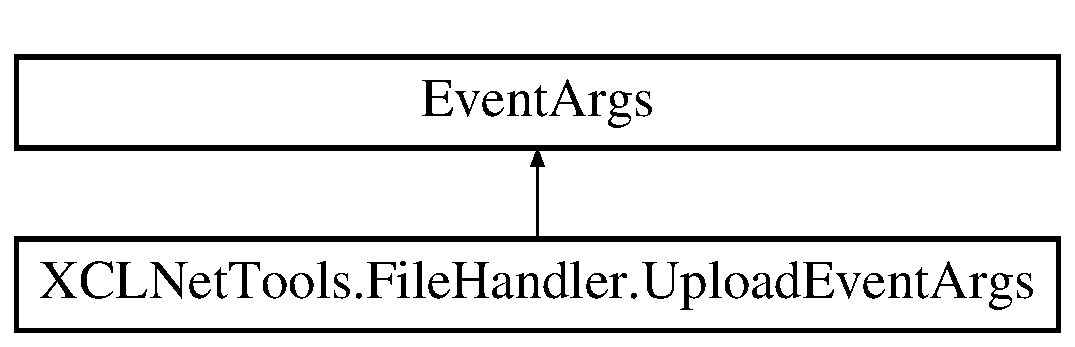
\includegraphics[height=2.000000cm]{class_x_c_l_net_tools_1_1_file_handler_1_1_upload_event_args}
\end{center}
\end{figure}
\subsection*{属性}
\begin{DoxyCompactItemize}
\item 
int \hyperlink{class_x_c_l_net_tools_1_1_file_handler_1_1_upload_event_args_aeb753c87413d86d610121060635794e1}{Bytes\+Sent}\hspace{0.3cm}{\ttfamily  \mbox{[}get, set\mbox{]}}
\begin{DoxyCompactList}\small\item\em 已发送的字节数 \end{DoxyCompactList}\item 
int \hyperlink{class_x_c_l_net_tools_1_1_file_handler_1_1_upload_event_args_a874a8bc16016a3d11eb9aa52f9670eb4}{Total\+Bytes}\hspace{0.3cm}{\ttfamily  \mbox{[}get, set\mbox{]}}
\begin{DoxyCompactList}\small\item\em 总字节数 \end{DoxyCompactList}\end{DoxyCompactItemize}


\subsection{详细描述}
上传数据参数 



在文件 Http\+Proc.\+cs 第 23 行定义.



\subsection{属性说明}
\index{X\+C\+L\+Net\+Tools\+::\+File\+Handler\+::\+Upload\+Event\+Args@{X\+C\+L\+Net\+Tools\+::\+File\+Handler\+::\+Upload\+Event\+Args}!Bytes\+Sent@{Bytes\+Sent}}
\index{Bytes\+Sent@{Bytes\+Sent}!X\+C\+L\+Net\+Tools\+::\+File\+Handler\+::\+Upload\+Event\+Args@{X\+C\+L\+Net\+Tools\+::\+File\+Handler\+::\+Upload\+Event\+Args}}
\subsubsection[{\texorpdfstring{Bytes\+Sent}{BytesSent}}]{\setlength{\rightskip}{0pt plus 5cm}int X\+C\+L\+Net\+Tools.\+File\+Handler.\+Upload\+Event\+Args.\+Bytes\+Sent\hspace{0.3cm}{\ttfamily [get]}, {\ttfamily [set]}}\hypertarget{class_x_c_l_net_tools_1_1_file_handler_1_1_upload_event_args_aeb753c87413d86d610121060635794e1}{}\label{class_x_c_l_net_tools_1_1_file_handler_1_1_upload_event_args_aeb753c87413d86d610121060635794e1}


已发送的字节数 



在文件 Http\+Proc.\+cs 第 32 行定义.

\index{X\+C\+L\+Net\+Tools\+::\+File\+Handler\+::\+Upload\+Event\+Args@{X\+C\+L\+Net\+Tools\+::\+File\+Handler\+::\+Upload\+Event\+Args}!Total\+Bytes@{Total\+Bytes}}
\index{Total\+Bytes@{Total\+Bytes}!X\+C\+L\+Net\+Tools\+::\+File\+Handler\+::\+Upload\+Event\+Args@{X\+C\+L\+Net\+Tools\+::\+File\+Handler\+::\+Upload\+Event\+Args}}
\subsubsection[{\texorpdfstring{Total\+Bytes}{TotalBytes}}]{\setlength{\rightskip}{0pt plus 5cm}int X\+C\+L\+Net\+Tools.\+File\+Handler.\+Upload\+Event\+Args.\+Total\+Bytes\hspace{0.3cm}{\ttfamily [get]}, {\ttfamily [set]}}\hypertarget{class_x_c_l_net_tools_1_1_file_handler_1_1_upload_event_args_a874a8bc16016a3d11eb9aa52f9670eb4}{}\label{class_x_c_l_net_tools_1_1_file_handler_1_1_upload_event_args_a874a8bc16016a3d11eb9aa52f9670eb4}


总字节数 



在文件 Http\+Proc.\+cs 第 41 行定义.



该类的文档由以下文件生成\+:\begin{DoxyCompactItemize}
\item 
E\+:/\+Git\+Hub/\+X\+C\+L\+Net\+Tools/\+X\+C\+L\+Net\+Tools/\+File\+Handler/\hyperlink{_http_proc_8cs}{Http\+Proc.\+cs}\end{DoxyCompactItemize}

\hypertarget{class_x_c_l_net_tools_1_1_file_handler_1_1_web_client}{}\section{X\+C\+L\+Net\+Tools.\+File\+Handler.\+Web\+Client类 参考}
\label{class_x_c_l_net_tools_1_1_file_handler_1_1_web_client}\index{X\+C\+L\+Net\+Tools.\+File\+Handler.\+Web\+Client@{X\+C\+L\+Net\+Tools.\+File\+Handler.\+Web\+Client}}


\hyperlink{class_x_c_l_net_tools_1_1_file_handler_1_1_web_client}{Web\+Client}  


\subsection*{Public 成员函数}
\begin{DoxyCompactItemize}
\item 
\hyperlink{class_x_c_l_net_tools_1_1_file_handler_1_1_web_client_a8f3cbaf1baf5d142caab2f6c9cc04a7f}{Web\+Client} ()
\begin{DoxyCompactList}\small\item\em 创建\+Web\+Client的实例 \end{DoxyCompactList}\item 
string \hyperlink{class_x_c_l_net_tools_1_1_file_handler_1_1_web_client_a504910f5e28a6fa620853f069d3c756b}{Get\+Html} (string url)
\begin{DoxyCompactList}\small\item\em 获取网页源代码 \end{DoxyCompactList}\item 
void \hyperlink{class_x_c_l_net_tools_1_1_file_handler_1_1_web_client_ace80aaf94d3e0c6eceb3ad182b8de947}{Download\+File} (string url, string filename)
\begin{DoxyCompactList}\small\item\em 下载文件 \end{DoxyCompactList}\item 
byte \mbox{[}$\,$\mbox{]} \hyperlink{class_x_c_l_net_tools_1_1_file_handler_1_1_web_client_a7208770077f210c3dd7bee2b34f0a4eb}{Get\+Data} (string url)
\begin{DoxyCompactList}\small\item\em 从指定\+U\+R\+L下载数据 \end{DoxyCompactList}\item 
string \hyperlink{class_x_c_l_net_tools_1_1_file_handler_1_1_web_client_ab2497ff9ed5a5b867362b7bc0b38edb1}{Post} (string url, string post\+Data)
\begin{DoxyCompactList}\small\item\em 向指定\+U\+R\+L发送文本数据 \end{DoxyCompactList}\item 
string \hyperlink{class_x_c_l_net_tools_1_1_file_handler_1_1_web_client_ad799cba2f787fba4c0ca4fc6e86ee831}{Post} (string url, byte\mbox{[}$\,$\mbox{]} post\+Data)
\begin{DoxyCompactList}\small\item\em 向指定\+U\+R\+L发送字节数据 \end{DoxyCompactList}\item 
string \hyperlink{class_x_c_l_net_tools_1_1_file_handler_1_1_web_client_ab1556a7a601a8425c7d6bcecb09d6cf2}{Post} (string url, \hyperlink{class_x_c_l_net_tools_1_1_file_handler_1_1_multipart_form}{Multipart\+Form} mulitpart\+Form)
\begin{DoxyCompactList}\small\item\em 向指定网址发送mulitpart编码的数据 \end{DoxyCompactList}\end{DoxyCompactItemize}
\subsection*{属性}
\begin{DoxyCompactItemize}
\item 
int \hyperlink{class_x_c_l_net_tools_1_1_file_handler_1_1_web_client_a192f27c95b8274758ca9d68c620de7c3}{Buffer\+Size}\hspace{0.3cm}{\ttfamily  \mbox{[}get, set\mbox{]}}
\begin{DoxyCompactList}\small\item\em 设置发送和接收的数据缓冲大小 \end{DoxyCompactList}\item 
Web\+Header\+Collection \hyperlink{class_x_c_l_net_tools_1_1_file_handler_1_1_web_client_a3d00d3457c23ce30274af963f4cab6bb}{Response\+Headers}\hspace{0.3cm}{\ttfamily  \mbox{[}get\mbox{]}}
\begin{DoxyCompactList}\small\item\em 获取响应头集合 \end{DoxyCompactList}\item 
Web\+Header\+Collection \hyperlink{class_x_c_l_net_tools_1_1_file_handler_1_1_web_client_a89d4bf2af70a2a0991904b1b61c8dd1d}{Request\+Headers}\hspace{0.3cm}{\ttfamily  \mbox{[}get\mbox{]}}
\begin{DoxyCompactList}\small\item\em 获取请求头集合 \end{DoxyCompactList}\item 
Web\+Proxy \hyperlink{class_x_c_l_net_tools_1_1_file_handler_1_1_web_client_ac2f17eefdc2372eb01a6be915d19c0ba}{Proxy}\hspace{0.3cm}{\ttfamily  \mbox{[}get, set\mbox{]}}
\begin{DoxyCompactList}\small\item\em 获取或设置代理 \end{DoxyCompactList}\item 
Encoding \hyperlink{class_x_c_l_net_tools_1_1_file_handler_1_1_web_client_a9bd02ab7f0198d34a44487c5d8c02f19}{Encoding}\hspace{0.3cm}{\ttfamily  \mbox{[}get, set\mbox{]}}
\begin{DoxyCompactList}\small\item\em 获取或设置请求与响应的文本编码方式 \end{DoxyCompactList}\item 
string \hyperlink{class_x_c_l_net_tools_1_1_file_handler_1_1_web_client_a67e90e96bd067171c16cb84d75f66c3a}{Resp\+Html}\hspace{0.3cm}{\ttfamily  \mbox{[}get, set\mbox{]}}
\begin{DoxyCompactList}\small\item\em 获取或设置响应的html代码 \end{DoxyCompactList}\item 
Cookie\+Container \hyperlink{class_x_c_l_net_tools_1_1_file_handler_1_1_web_client_adeaa1201074e43df3743d76ea77cf06e}{Cookie\+Container}\hspace{0.3cm}{\ttfamily  \mbox{[}get, set\mbox{]}}
\begin{DoxyCompactList}\small\item\em 获取或设置与请求关联的\+Cookie容器 \end{DoxyCompactList}\end{DoxyCompactItemize}
\subsection*{事件}
\begin{DoxyCompactItemize}
\item 
Event\+Handler$<$ \hyperlink{class_x_c_l_net_tools_1_1_file_handler_1_1_upload_event_args}{Upload\+Event\+Args} $>$ \hyperlink{class_x_c_l_net_tools_1_1_file_handler_1_1_web_client_abe950fa329508b4c52e3181aeb97585f}{Upload\+Progress\+Changed}
\begin{DoxyCompactList}\small\item\em 上传事件 \end{DoxyCompactList}\item 
Event\+Handler$<$ \hyperlink{class_x_c_l_net_tools_1_1_file_handler_1_1_download_event_args}{Download\+Event\+Args} $>$ \hyperlink{class_x_c_l_net_tools_1_1_file_handler_1_1_web_client_aa1e50d608381b728356547eff9f80213}{Download\+Progress\+Changed}
\begin{DoxyCompactList}\small\item\em 下载事件 \end{DoxyCompactList}\end{DoxyCompactItemize}


\subsection{详细描述}
\hyperlink{class_x_c_l_net_tools_1_1_file_handler_1_1_web_client}{Web\+Client} 



在文件 Http\+Proc.\+cs 第 87 行定义.



\subsection{构造及析构函数说明}
\mbox{\Hypertarget{class_x_c_l_net_tools_1_1_file_handler_1_1_web_client_a8f3cbaf1baf5d142caab2f6c9cc04a7f}\label{class_x_c_l_net_tools_1_1_file_handler_1_1_web_client_a8f3cbaf1baf5d142caab2f6c9cc04a7f}} 
\index{X\+C\+L\+Net\+Tools\+::\+File\+Handler\+::\+Web\+Client@{X\+C\+L\+Net\+Tools\+::\+File\+Handler\+::\+Web\+Client}!Web\+Client@{Web\+Client}}
\index{Web\+Client@{Web\+Client}!X\+C\+L\+Net\+Tools\+::\+File\+Handler\+::\+Web\+Client@{X\+C\+L\+Net\+Tools\+::\+File\+Handler\+::\+Web\+Client}}
\subsubsection{\texorpdfstring{Web\+Client()}{WebClient()}}
{\footnotesize\ttfamily X\+C\+L\+Net\+Tools.\+File\+Handler.\+Web\+Client.\+Web\+Client (\begin{DoxyParamCaption}{ }\end{DoxyParamCaption})}



创建\+Web\+Client的实例 



在文件 Http\+Proc.\+cs 第 115 行定义.



\subsection{成员函数说明}
\mbox{\Hypertarget{class_x_c_l_net_tools_1_1_file_handler_1_1_web_client_ace80aaf94d3e0c6eceb3ad182b8de947}\label{class_x_c_l_net_tools_1_1_file_handler_1_1_web_client_ace80aaf94d3e0c6eceb3ad182b8de947}} 
\index{X\+C\+L\+Net\+Tools\+::\+File\+Handler\+::\+Web\+Client@{X\+C\+L\+Net\+Tools\+::\+File\+Handler\+::\+Web\+Client}!Download\+File@{Download\+File}}
\index{Download\+File@{Download\+File}!X\+C\+L\+Net\+Tools\+::\+File\+Handler\+::\+Web\+Client@{X\+C\+L\+Net\+Tools\+::\+File\+Handler\+::\+Web\+Client}}
\subsubsection{\texorpdfstring{Download\+File()}{DownloadFile()}}
{\footnotesize\ttfamily void X\+C\+L\+Net\+Tools.\+File\+Handler.\+Web\+Client.\+Download\+File (\begin{DoxyParamCaption}\item[{string}]{url,  }\item[{string}]{filename }\end{DoxyParamCaption})}



下载文件 


\begin{DoxyParams}{参数}
{\em url} & 文件\+U\+R\+L地址\\
\hline
{\em filename} & 文件保存完整路径\\
\hline
\end{DoxyParams}


在文件 Http\+Proc.\+cs 第 199 行定义.

\mbox{\Hypertarget{class_x_c_l_net_tools_1_1_file_handler_1_1_web_client_a7208770077f210c3dd7bee2b34f0a4eb}\label{class_x_c_l_net_tools_1_1_file_handler_1_1_web_client_a7208770077f210c3dd7bee2b34f0a4eb}} 
\index{X\+C\+L\+Net\+Tools\+::\+File\+Handler\+::\+Web\+Client@{X\+C\+L\+Net\+Tools\+::\+File\+Handler\+::\+Web\+Client}!Get\+Data@{Get\+Data}}
\index{Get\+Data@{Get\+Data}!X\+C\+L\+Net\+Tools\+::\+File\+Handler\+::\+Web\+Client@{X\+C\+L\+Net\+Tools\+::\+File\+Handler\+::\+Web\+Client}}
\subsubsection{\texorpdfstring{Get\+Data()}{GetData()}}
{\footnotesize\ttfamily byte \mbox{[}$\,$\mbox{]} X\+C\+L\+Net\+Tools.\+File\+Handler.\+Web\+Client.\+Get\+Data (\begin{DoxyParamCaption}\item[{string}]{url }\end{DoxyParamCaption})}



从指定\+U\+R\+L下载数据 


\begin{DoxyParams}{参数}
{\em url} & 网址\\
\hline
\end{DoxyParams}
\begin{DoxyReturn}{返回}

\end{DoxyReturn}


在文件 Http\+Proc.\+cs 第 220 行定义.

\mbox{\Hypertarget{class_x_c_l_net_tools_1_1_file_handler_1_1_web_client_a504910f5e28a6fa620853f069d3c756b}\label{class_x_c_l_net_tools_1_1_file_handler_1_1_web_client_a504910f5e28a6fa620853f069d3c756b}} 
\index{X\+C\+L\+Net\+Tools\+::\+File\+Handler\+::\+Web\+Client@{X\+C\+L\+Net\+Tools\+::\+File\+Handler\+::\+Web\+Client}!Get\+Html@{Get\+Html}}
\index{Get\+Html@{Get\+Html}!X\+C\+L\+Net\+Tools\+::\+File\+Handler\+::\+Web\+Client@{X\+C\+L\+Net\+Tools\+::\+File\+Handler\+::\+Web\+Client}}
\subsubsection{\texorpdfstring{Get\+Html()}{GetHtml()}}
{\footnotesize\ttfamily string X\+C\+L\+Net\+Tools.\+File\+Handler.\+Web\+Client.\+Get\+Html (\begin{DoxyParamCaption}\item[{string}]{url }\end{DoxyParamCaption})}



获取网页源代码 


\begin{DoxyParams}{参数}
{\em url} & 网址\\
\hline
\end{DoxyParams}
\begin{DoxyReturn}{返回}

\end{DoxyReturn}


在文件 Http\+Proc.\+cs 第 187 行定义.

\mbox{\Hypertarget{class_x_c_l_net_tools_1_1_file_handler_1_1_web_client_ab2497ff9ed5a5b867362b7bc0b38edb1}\label{class_x_c_l_net_tools_1_1_file_handler_1_1_web_client_ab2497ff9ed5a5b867362b7bc0b38edb1}} 
\index{X\+C\+L\+Net\+Tools\+::\+File\+Handler\+::\+Web\+Client@{X\+C\+L\+Net\+Tools\+::\+File\+Handler\+::\+Web\+Client}!Post@{Post}}
\index{Post@{Post}!X\+C\+L\+Net\+Tools\+::\+File\+Handler\+::\+Web\+Client@{X\+C\+L\+Net\+Tools\+::\+File\+Handler\+::\+Web\+Client}}
\subsubsection{\texorpdfstring{Post()}{Post()}\hspace{0.1cm}{\footnotesize\ttfamily [1/3]}}
{\footnotesize\ttfamily string X\+C\+L\+Net\+Tools.\+File\+Handler.\+Web\+Client.\+Post (\begin{DoxyParamCaption}\item[{string}]{url,  }\item[{string}]{post\+Data }\end{DoxyParamCaption})}



向指定\+U\+R\+L发送文本数据 


\begin{DoxyParams}{参数}
{\em url} & 网址\\
\hline
{\em post\+Data} & urlencode编码的文本数据\\
\hline
\end{DoxyParams}
\begin{DoxyReturn}{返回}

\end{DoxyReturn}


在文件 Http\+Proc.\+cs 第 232 行定义.

\mbox{\Hypertarget{class_x_c_l_net_tools_1_1_file_handler_1_1_web_client_ad799cba2f787fba4c0ca4fc6e86ee831}\label{class_x_c_l_net_tools_1_1_file_handler_1_1_web_client_ad799cba2f787fba4c0ca4fc6e86ee831}} 
\index{X\+C\+L\+Net\+Tools\+::\+File\+Handler\+::\+Web\+Client@{X\+C\+L\+Net\+Tools\+::\+File\+Handler\+::\+Web\+Client}!Post@{Post}}
\index{Post@{Post}!X\+C\+L\+Net\+Tools\+::\+File\+Handler\+::\+Web\+Client@{X\+C\+L\+Net\+Tools\+::\+File\+Handler\+::\+Web\+Client}}
\subsubsection{\texorpdfstring{Post()}{Post()}\hspace{0.1cm}{\footnotesize\ttfamily [2/3]}}
{\footnotesize\ttfamily string X\+C\+L\+Net\+Tools.\+File\+Handler.\+Web\+Client.\+Post (\begin{DoxyParamCaption}\item[{string}]{url,  }\item[{byte \mbox{[}$\,$\mbox{]}}]{post\+Data }\end{DoxyParamCaption})}



向指定\+U\+R\+L发送字节数据 


\begin{DoxyParams}{参数}
{\em url} & 网址\\
\hline
{\em post\+Data} & 发送的字节数组\\
\hline
\end{DoxyParams}
\begin{DoxyReturn}{返回}

\end{DoxyReturn}


在文件 Http\+Proc.\+cs 第 244 行定义.

\mbox{\Hypertarget{class_x_c_l_net_tools_1_1_file_handler_1_1_web_client_ab1556a7a601a8425c7d6bcecb09d6cf2}\label{class_x_c_l_net_tools_1_1_file_handler_1_1_web_client_ab1556a7a601a8425c7d6bcecb09d6cf2}} 
\index{X\+C\+L\+Net\+Tools\+::\+File\+Handler\+::\+Web\+Client@{X\+C\+L\+Net\+Tools\+::\+File\+Handler\+::\+Web\+Client}!Post@{Post}}
\index{Post@{Post}!X\+C\+L\+Net\+Tools\+::\+File\+Handler\+::\+Web\+Client@{X\+C\+L\+Net\+Tools\+::\+File\+Handler\+::\+Web\+Client}}
\subsubsection{\texorpdfstring{Post()}{Post()}\hspace{0.1cm}{\footnotesize\ttfamily [3/3]}}
{\footnotesize\ttfamily string X\+C\+L\+Net\+Tools.\+File\+Handler.\+Web\+Client.\+Post (\begin{DoxyParamCaption}\item[{string}]{url,  }\item[{\hyperlink{class_x_c_l_net_tools_1_1_file_handler_1_1_multipart_form}{Multipart\+Form}}]{mulitpart\+Form }\end{DoxyParamCaption})}



向指定网址发送mulitpart编码的数据 


\begin{DoxyParams}{参数}
{\em url} & 网址\\
\hline
{\em mulitpart\+Form} & mulitpart form data\\
\hline
\end{DoxyParams}
\begin{DoxyReturn}{返回}

\end{DoxyReturn}


在文件 Http\+Proc.\+cs 第 261 行定义.



\subsection{属性说明}
\mbox{\Hypertarget{class_x_c_l_net_tools_1_1_file_handler_1_1_web_client_a192f27c95b8274758ca9d68c620de7c3}\label{class_x_c_l_net_tools_1_1_file_handler_1_1_web_client_a192f27c95b8274758ca9d68c620de7c3}} 
\index{X\+C\+L\+Net\+Tools\+::\+File\+Handler\+::\+Web\+Client@{X\+C\+L\+Net\+Tools\+::\+File\+Handler\+::\+Web\+Client}!Buffer\+Size@{Buffer\+Size}}
\index{Buffer\+Size@{Buffer\+Size}!X\+C\+L\+Net\+Tools\+::\+File\+Handler\+::\+Web\+Client@{X\+C\+L\+Net\+Tools\+::\+File\+Handler\+::\+Web\+Client}}
\subsubsection{\texorpdfstring{Buffer\+Size}{BufferSize}}
{\footnotesize\ttfamily int X\+C\+L\+Net\+Tools.\+File\+Handler.\+Web\+Client.\+Buffer\+Size\hspace{0.3cm}{\ttfamily [get]}, {\ttfamily [set]}}



设置发送和接收的数据缓冲大小 



在文件 Http\+Proc.\+cs 第 125 行定义.

\mbox{\Hypertarget{class_x_c_l_net_tools_1_1_file_handler_1_1_web_client_adeaa1201074e43df3743d76ea77cf06e}\label{class_x_c_l_net_tools_1_1_file_handler_1_1_web_client_adeaa1201074e43df3743d76ea77cf06e}} 
\index{X\+C\+L\+Net\+Tools\+::\+File\+Handler\+::\+Web\+Client@{X\+C\+L\+Net\+Tools\+::\+File\+Handler\+::\+Web\+Client}!Cookie\+Container@{Cookie\+Container}}
\index{Cookie\+Container@{Cookie\+Container}!X\+C\+L\+Net\+Tools\+::\+File\+Handler\+::\+Web\+Client@{X\+C\+L\+Net\+Tools\+::\+File\+Handler\+::\+Web\+Client}}
\subsubsection{\texorpdfstring{Cookie\+Container}{CookieContainer}}
{\footnotesize\ttfamily Cookie\+Container X\+C\+L\+Net\+Tools.\+File\+Handler.\+Web\+Client.\+Cookie\+Container\hspace{0.3cm}{\ttfamily [get]}, {\ttfamily [set]}}



获取或设置与请求关联的\+Cookie容器 



在文件 Http\+Proc.\+cs 第 177 行定义.

\mbox{\Hypertarget{class_x_c_l_net_tools_1_1_file_handler_1_1_web_client_a9bd02ab7f0198d34a44487c5d8c02f19}\label{class_x_c_l_net_tools_1_1_file_handler_1_1_web_client_a9bd02ab7f0198d34a44487c5d8c02f19}} 
\index{X\+C\+L\+Net\+Tools\+::\+File\+Handler\+::\+Web\+Client@{X\+C\+L\+Net\+Tools\+::\+File\+Handler\+::\+Web\+Client}!Encoding@{Encoding}}
\index{Encoding@{Encoding}!X\+C\+L\+Net\+Tools\+::\+File\+Handler\+::\+Web\+Client@{X\+C\+L\+Net\+Tools\+::\+File\+Handler\+::\+Web\+Client}}
\subsubsection{\texorpdfstring{Encoding}{Encoding}}
{\footnotesize\ttfamily Encoding X\+C\+L\+Net\+Tools.\+File\+Handler.\+Web\+Client.\+Encoding\hspace{0.3cm}{\ttfamily [get]}, {\ttfamily [set]}}



获取或设置请求与响应的文本编码方式 



在文件 Http\+Proc.\+cs 第 159 行定义.

\mbox{\Hypertarget{class_x_c_l_net_tools_1_1_file_handler_1_1_web_client_ac2f17eefdc2372eb01a6be915d19c0ba}\label{class_x_c_l_net_tools_1_1_file_handler_1_1_web_client_ac2f17eefdc2372eb01a6be915d19c0ba}} 
\index{X\+C\+L\+Net\+Tools\+::\+File\+Handler\+::\+Web\+Client@{X\+C\+L\+Net\+Tools\+::\+File\+Handler\+::\+Web\+Client}!Proxy@{Proxy}}
\index{Proxy@{Proxy}!X\+C\+L\+Net\+Tools\+::\+File\+Handler\+::\+Web\+Client@{X\+C\+L\+Net\+Tools\+::\+File\+Handler\+::\+Web\+Client}}
\subsubsection{\texorpdfstring{Proxy}{Proxy}}
{\footnotesize\ttfamily Web\+Proxy X\+C\+L\+Net\+Tools.\+File\+Handler.\+Web\+Client.\+Proxy\hspace{0.3cm}{\ttfamily [get]}, {\ttfamily [set]}}



获取或设置代理 



在文件 Http\+Proc.\+cs 第 150 行定义.

\mbox{\Hypertarget{class_x_c_l_net_tools_1_1_file_handler_1_1_web_client_a89d4bf2af70a2a0991904b1b61c8dd1d}\label{class_x_c_l_net_tools_1_1_file_handler_1_1_web_client_a89d4bf2af70a2a0991904b1b61c8dd1d}} 
\index{X\+C\+L\+Net\+Tools\+::\+File\+Handler\+::\+Web\+Client@{X\+C\+L\+Net\+Tools\+::\+File\+Handler\+::\+Web\+Client}!Request\+Headers@{Request\+Headers}}
\index{Request\+Headers@{Request\+Headers}!X\+C\+L\+Net\+Tools\+::\+File\+Handler\+::\+Web\+Client@{X\+C\+L\+Net\+Tools\+::\+File\+Handler\+::\+Web\+Client}}
\subsubsection{\texorpdfstring{Request\+Headers}{RequestHeaders}}
{\footnotesize\ttfamily Web\+Header\+Collection X\+C\+L\+Net\+Tools.\+File\+Handler.\+Web\+Client.\+Request\+Headers\hspace{0.3cm}{\ttfamily [get]}}



获取请求头集合 



在文件 Http\+Proc.\+cs 第 142 行定义.

\mbox{\Hypertarget{class_x_c_l_net_tools_1_1_file_handler_1_1_web_client_a67e90e96bd067171c16cb84d75f66c3a}\label{class_x_c_l_net_tools_1_1_file_handler_1_1_web_client_a67e90e96bd067171c16cb84d75f66c3a}} 
\index{X\+C\+L\+Net\+Tools\+::\+File\+Handler\+::\+Web\+Client@{X\+C\+L\+Net\+Tools\+::\+File\+Handler\+::\+Web\+Client}!Resp\+Html@{Resp\+Html}}
\index{Resp\+Html@{Resp\+Html}!X\+C\+L\+Net\+Tools\+::\+File\+Handler\+::\+Web\+Client@{X\+C\+L\+Net\+Tools\+::\+File\+Handler\+::\+Web\+Client}}
\subsubsection{\texorpdfstring{Resp\+Html}{RespHtml}}
{\footnotesize\ttfamily string X\+C\+L\+Net\+Tools.\+File\+Handler.\+Web\+Client.\+Resp\+Html\hspace{0.3cm}{\ttfamily [get]}, {\ttfamily [set]}}



获取或设置响应的html代码 



在文件 Http\+Proc.\+cs 第 168 行定义.

\mbox{\Hypertarget{class_x_c_l_net_tools_1_1_file_handler_1_1_web_client_a3d00d3457c23ce30274af963f4cab6bb}\label{class_x_c_l_net_tools_1_1_file_handler_1_1_web_client_a3d00d3457c23ce30274af963f4cab6bb}} 
\index{X\+C\+L\+Net\+Tools\+::\+File\+Handler\+::\+Web\+Client@{X\+C\+L\+Net\+Tools\+::\+File\+Handler\+::\+Web\+Client}!Response\+Headers@{Response\+Headers}}
\index{Response\+Headers@{Response\+Headers}!X\+C\+L\+Net\+Tools\+::\+File\+Handler\+::\+Web\+Client@{X\+C\+L\+Net\+Tools\+::\+File\+Handler\+::\+Web\+Client}}
\subsubsection{\texorpdfstring{Response\+Headers}{ResponseHeaders}}
{\footnotesize\ttfamily Web\+Header\+Collection X\+C\+L\+Net\+Tools.\+File\+Handler.\+Web\+Client.\+Response\+Headers\hspace{0.3cm}{\ttfamily [get]}}



获取响应头集合 



在文件 Http\+Proc.\+cs 第 134 行定义.



\subsection{事件说明}
\mbox{\Hypertarget{class_x_c_l_net_tools_1_1_file_handler_1_1_web_client_aa1e50d608381b728356547eff9f80213}\label{class_x_c_l_net_tools_1_1_file_handler_1_1_web_client_aa1e50d608381b728356547eff9f80213}} 
\index{X\+C\+L\+Net\+Tools\+::\+File\+Handler\+::\+Web\+Client@{X\+C\+L\+Net\+Tools\+::\+File\+Handler\+::\+Web\+Client}!Download\+Progress\+Changed@{Download\+Progress\+Changed}}
\index{Download\+Progress\+Changed@{Download\+Progress\+Changed}!X\+C\+L\+Net\+Tools\+::\+File\+Handler\+::\+Web\+Client@{X\+C\+L\+Net\+Tools\+::\+File\+Handler\+::\+Web\+Client}}
\subsubsection{\texorpdfstring{Download\+Progress\+Changed}{DownloadProgressChanged}}
{\footnotesize\ttfamily Event\+Handler$<$\hyperlink{class_x_c_l_net_tools_1_1_file_handler_1_1_download_event_args}{Download\+Event\+Args}$>$ X\+C\+L\+Net\+Tools.\+File\+Handler.\+Web\+Client.\+Download\+Progress\+Changed}



下载事件 



在文件 Http\+Proc.\+cs 第 105 行定义.

\mbox{\Hypertarget{class_x_c_l_net_tools_1_1_file_handler_1_1_web_client_abe950fa329508b4c52e3181aeb97585f}\label{class_x_c_l_net_tools_1_1_file_handler_1_1_web_client_abe950fa329508b4c52e3181aeb97585f}} 
\index{X\+C\+L\+Net\+Tools\+::\+File\+Handler\+::\+Web\+Client@{X\+C\+L\+Net\+Tools\+::\+File\+Handler\+::\+Web\+Client}!Upload\+Progress\+Changed@{Upload\+Progress\+Changed}}
\index{Upload\+Progress\+Changed@{Upload\+Progress\+Changed}!X\+C\+L\+Net\+Tools\+::\+File\+Handler\+::\+Web\+Client@{X\+C\+L\+Net\+Tools\+::\+File\+Handler\+::\+Web\+Client}}
\subsubsection{\texorpdfstring{Upload\+Progress\+Changed}{UploadProgressChanged}}
{\footnotesize\ttfamily Event\+Handler$<$\hyperlink{class_x_c_l_net_tools_1_1_file_handler_1_1_upload_event_args}{Upload\+Event\+Args}$>$ X\+C\+L\+Net\+Tools.\+File\+Handler.\+Web\+Client.\+Upload\+Progress\+Changed}



上传事件 



在文件 Http\+Proc.\+cs 第 100 行定义.



该类的文档由以下文件生成\+:\begin{DoxyCompactItemize}
\item 
D\+:/\+My\+Data/\+Git\+Hub/\+X\+C\+L\+Net\+Tools/\+X\+C\+L\+Net\+Tools/\+File\+Handler/\hyperlink{_http_proc_8cs}{Http\+Proc.\+cs}\end{DoxyCompactItemize}

\chapter{文件说明}
\hypertarget{_cache_class_8cs}{}\section{D\+:/\+My\+Data/\+Git\+Hub/\+X\+C\+L\+Net\+Tools/\+X\+C\+L\+Net\+Tools/\+Cache/\+Cache\+Class.cs 文件参考}
\label{_cache_class_8cs}\index{D\+:/\+My\+Data/\+Git\+Hub/\+X\+C\+L\+Net\+Tools/\+X\+C\+L\+Net\+Tools/\+Cache/\+Cache\+Class.\+cs@{D\+:/\+My\+Data/\+Git\+Hub/\+X\+C\+L\+Net\+Tools/\+X\+C\+L\+Net\+Tools/\+Cache/\+Cache\+Class.\+cs}}
\subsection*{类}
\begin{DoxyCompactItemize}
\item 
class \hyperlink{class_x_c_l_net_tools_1_1_cache_1_1_cache_class}{X\+C\+L\+Net\+Tools.\+Cache.\+Cache\+Class}
\begin{DoxyCompactList}\small\item\em 缓存相关的操作类 \end{DoxyCompactList}\end{DoxyCompactItemize}
\subsection*{命名空间}
\begin{DoxyCompactItemize}
\item 
namespace \hyperlink{namespace_x_c_l_net_tools_1_1_cache}{X\+C\+L\+Net\+Tools.\+Cache}
\end{DoxyCompactItemize}

\hypertarget{_consts_8cs}{}\section{D\+:/\+My\+Data/\+Git\+Hub/\+X\+C\+L\+Net\+Tools/\+X\+C\+L\+Net\+Tools/\+Common/\+Consts.cs 文件参考}
\label{_consts_8cs}\index{D\+:/\+My\+Data/\+Git\+Hub/\+X\+C\+L\+Net\+Tools/\+X\+C\+L\+Net\+Tools/\+Common/\+Consts.\+cs@{D\+:/\+My\+Data/\+Git\+Hub/\+X\+C\+L\+Net\+Tools/\+X\+C\+L\+Net\+Tools/\+Common/\+Consts.\+cs}}
\subsection*{类}
\begin{DoxyCompactItemize}
\item 
class {\bfseries X\+C\+L\+Net\+Tools.\+Common.\+Consts}
\begin{DoxyCompactList}\small\item\em 常量 \end{DoxyCompactList}\end{DoxyCompactItemize}
\subsection*{命名空间}
\begin{DoxyCompactItemize}
\item 
namespace \hyperlink{namespace_x_c_l_net_tools_1_1_common}{X\+C\+L\+Net\+Tools.\+Common}
\end{DoxyCompactItemize}

\hypertarget{_data_type_convert_8cs}{}\section{D\+:/\+My\+Data/\+Git\+Hub/\+X\+C\+L\+Net\+Tools/\+X\+C\+L\+Net\+Tools/\+Common/\+Data\+Type\+Convert.cs 文件参考}
\label{_data_type_convert_8cs}\index{D\+:/\+My\+Data/\+Git\+Hub/\+X\+C\+L\+Net\+Tools/\+X\+C\+L\+Net\+Tools/\+Common/\+Data\+Type\+Convert.\+cs@{D\+:/\+My\+Data/\+Git\+Hub/\+X\+C\+L\+Net\+Tools/\+X\+C\+L\+Net\+Tools/\+Common/\+Data\+Type\+Convert.\+cs}}
\subsection*{类}
\begin{DoxyCompactItemize}
\item 
class \hyperlink{class_x_c_l_net_tools_1_1_common_1_1_data_type_convert}{X\+C\+L\+Net\+Tools.\+Common.\+Data\+Type\+Convert}
\begin{DoxyCompactList}\small\item\em C\+::数据类型转换 \end{DoxyCompactList}\end{DoxyCompactItemize}
\subsection*{命名空间}
\begin{DoxyCompactItemize}
\item 
namespace \hyperlink{namespace_x_c_l_net_tools_1_1_common}{X\+C\+L\+Net\+Tools.\+Common}
\end{DoxyCompactItemize}

\hypertarget{_g_zip_helper_8cs}{}\section{D\+:/\+My\+Data/\+Git\+Hub/\+X\+C\+L\+Net\+Tools/\+X\+C\+L\+Net\+Tools/\+Common/\+G\+Zip\+Helper.cs 文件参考}
\label{_g_zip_helper_8cs}\index{D\+:/\+My\+Data/\+Git\+Hub/\+X\+C\+L\+Net\+Tools/\+X\+C\+L\+Net\+Tools/\+Common/\+G\+Zip\+Helper.\+cs@{D\+:/\+My\+Data/\+Git\+Hub/\+X\+C\+L\+Net\+Tools/\+X\+C\+L\+Net\+Tools/\+Common/\+G\+Zip\+Helper.\+cs}}
\subsection*{类}
\begin{DoxyCompactItemize}
\item 
class \hyperlink{class_x_c_l_net_tools_1_1_common_1_1_g_zip_helper}{X\+C\+L\+Net\+Tools.\+Common.\+G\+Zip\+Helper}
\begin{DoxyCompactList}\small\item\em gzip相关 \end{DoxyCompactList}\end{DoxyCompactItemize}
\subsection*{命名空间}
\begin{DoxyCompactItemize}
\item 
namespace \hyperlink{namespace_x_c_l_net_tools_1_1_common}{X\+C\+L\+Net\+Tools.\+Common}
\end{DoxyCompactItemize}

\hypertarget{_i_p_helper_8cs}{}\section{D\+:/\+My\+Data/\+Git\+Hub/\+X\+C\+L\+Net\+Tools/\+X\+C\+L\+Net\+Tools/\+Common/\+I\+P\+Helper.cs 文件参考}
\label{_i_p_helper_8cs}\index{D\+:/\+My\+Data/\+Git\+Hub/\+X\+C\+L\+Net\+Tools/\+X\+C\+L\+Net\+Tools/\+Common/\+I\+P\+Helper.\+cs@{D\+:/\+My\+Data/\+Git\+Hub/\+X\+C\+L\+Net\+Tools/\+X\+C\+L\+Net\+Tools/\+Common/\+I\+P\+Helper.\+cs}}
\subsection*{类}
\begin{DoxyCompactItemize}
\item 
class {\bfseries X\+C\+L\+Net\+Tools.\+Common.\+I\+P\+Helper}
\begin{DoxyCompactList}\small\item\em I\+P处理 \end{DoxyCompactList}\end{DoxyCompactItemize}
\subsection*{命名空间}
\begin{DoxyCompactItemize}
\item 
namespace \hyperlink{namespace_x_c_l_net_tools_1_1_common}{X\+C\+L\+Net\+Tools.\+Common}
\end{DoxyCompactItemize}

\hypertarget{_switch_control_8cs}{}\section{D\+:/\+My\+Data/\+Git\+Hub/\+X\+C\+L\+Net\+Tools/\+X\+C\+L\+Net\+Tools/\+Common/\+Switch\+Control.cs 文件参考}
\label{_switch_control_8cs}\index{D\+:/\+My\+Data/\+Git\+Hub/\+X\+C\+L\+Net\+Tools/\+X\+C\+L\+Net\+Tools/\+Common/\+Switch\+Control.\+cs@{D\+:/\+My\+Data/\+Git\+Hub/\+X\+C\+L\+Net\+Tools/\+X\+C\+L\+Net\+Tools/\+Common/\+Switch\+Control.\+cs}}
\subsection*{类}
\begin{DoxyCompactItemize}
\item 
class \hyperlink{class_x_c_l_net_tools_1_1_common_1_1_switch_control}{X\+C\+L\+Net\+Tools.\+Common.\+Switch\+Control}
\begin{DoxyCompactList}\small\item\em 开关控制 \end{DoxyCompactList}\end{DoxyCompactItemize}
\subsection*{命名空间}
\begin{DoxyCompactItemize}
\item 
namespace \hyperlink{namespace_x_c_l_net_tools_1_1_common}{X\+C\+L\+Net\+Tools.\+Common}
\end{DoxyCompactItemize}

\hypertarget{_control_2_html_control_2_lib_8cs}{}\section{D\+:/\+My\+Data/\+Git\+Hub/\+X\+C\+L\+Net\+Tools/\+X\+C\+L\+Net\+Tools/\+Control/\+Html\+Control/\+Lib.cs 文件参考}
\label{_control_2_html_control_2_lib_8cs}\index{D\+:/\+My\+Data/\+Git\+Hub/\+X\+C\+L\+Net\+Tools/\+X\+C\+L\+Net\+Tools/\+Control/\+Html\+Control/\+Lib.\+cs@{D\+:/\+My\+Data/\+Git\+Hub/\+X\+C\+L\+Net\+Tools/\+X\+C\+L\+Net\+Tools/\+Control/\+Html\+Control/\+Lib.\+cs}}
\subsection*{类}
\begin{DoxyCompactItemize}
\item 
class {\bfseries X\+C\+L\+Net\+Tools.\+Control.\+Html\+Control.\+Lib}
\begin{DoxyCompactList}\small\item\em 原生html控件操作类 \end{DoxyCompactList}\end{DoxyCompactItemize}
\subsection*{命名空间}
\begin{DoxyCompactItemize}
\item 
namespace \hyperlink{namespace_x_c_l_net_tools_1_1_control_1_1_html_control}{X\+C\+L\+Net\+Tools.\+Control.\+Html\+Control}
\end{DoxyCompactItemize}

\hypertarget{_control_2_mx_graph_2_lib_8cs}{}\section{D\+:/\+My\+Data/\+Git\+Hub/\+X\+C\+L\+Net\+Tools/\+X\+C\+L\+Net\+Tools/\+Control/\+Mx\+Graph/\+Lib.cs 文件参考}
\label{_control_2_mx_graph_2_lib_8cs}\index{D\+:/\+My\+Data/\+Git\+Hub/\+X\+C\+L\+Net\+Tools/\+X\+C\+L\+Net\+Tools/\+Control/\+Mx\+Graph/\+Lib.\+cs@{D\+:/\+My\+Data/\+Git\+Hub/\+X\+C\+L\+Net\+Tools/\+X\+C\+L\+Net\+Tools/\+Control/\+Mx\+Graph/\+Lib.\+cs}}
\subsection*{类}
\begin{DoxyCompactItemize}
\item 
class \hyperlink{class_x_c_l_net_tools_1_1_control_1_1_mx_graph_1_1_lib}{X\+C\+L\+Net\+Tools.\+Control.\+Mx\+Graph.\+Lib}
\begin{DoxyCompactList}\small\item\em Mx\+Graph操作类 \end{DoxyCompactList}\end{DoxyCompactItemize}
\subsection*{命名空间}
\begin{DoxyCompactItemize}
\item 
namespace \hyperlink{namespace_x_c_l_net_tools_1_1_control_1_1_mx_graph}{X\+C\+L\+Net\+Tools.\+Control.\+Mx\+Graph}
\end{DoxyCompactItemize}

\hypertarget{_control_2_server_control_2_lib_8cs}{}\section{D\+:/\+My\+Data/\+Git\+Hub/\+X\+C\+L\+Net\+Tools/\+X\+C\+L\+Net\+Tools/\+Control/\+Server\+Control/\+Lib.cs 文件参考}
\label{_control_2_server_control_2_lib_8cs}\index{D\+:/\+My\+Data/\+Git\+Hub/\+X\+C\+L\+Net\+Tools/\+X\+C\+L\+Net\+Tools/\+Control/\+Server\+Control/\+Lib.\+cs@{D\+:/\+My\+Data/\+Git\+Hub/\+X\+C\+L\+Net\+Tools/\+X\+C\+L\+Net\+Tools/\+Control/\+Server\+Control/\+Lib.\+cs}}
\subsection*{类}
\begin{DoxyCompactItemize}
\item 
class \hyperlink{class_x_c_l_net_tools_1_1_control_1_1_server_control_1_1_lib}{X\+C\+L\+Net\+Tools.\+Control.\+Server\+Control.\+Lib}
\begin{DoxyCompactList}\small\item\em 服务器控件操作相关 \end{DoxyCompactList}\end{DoxyCompactItemize}
\subsection*{命名空间}
\begin{DoxyCompactItemize}
\item 
namespace \hyperlink{namespace_x_c_l_net_tools_1_1_control_1_1_server_control}{X\+C\+L\+Net\+Tools.\+Control.\+Server\+Control}
\end{DoxyCompactItemize}

\hypertarget{_encode_2_lib_8cs}{\section{D\-:/\-My\-Data/\-My\-Git/\-Git\-Hub/\-X\-C\-L\-Net\-Tools/\-X\-C\-L\-Net\-Tools/\-Encode/\-Lib.cs 文件参考}
\label{_encode_2_lib_8cs}\index{D\-:/\-My\-Data/\-My\-Git/\-Git\-Hub/\-X\-C\-L\-Net\-Tools/\-X\-C\-L\-Net\-Tools/\-Encode/\-Lib.\-cs@{D\-:/\-My\-Data/\-My\-Git/\-Git\-Hub/\-X\-C\-L\-Net\-Tools/\-X\-C\-L\-Net\-Tools/\-Encode/\-Lib.\-cs}}
}
\subsection*{类}
\begin{DoxyCompactItemize}
\item 
class \hyperlink{class_x_c_l_net_tools_1_1_encode_1_1_lib}{X\-C\-L\-Net\-Tools.\-Encode.\-Lib}
\begin{DoxyCompactList}\small\item\em 其它相关 \end{DoxyCompactList}\end{DoxyCompactItemize}
\subsection*{命名空间}
\begin{DoxyCompactItemize}
\item 
package \hyperlink{namespace_x_c_l_net_tools_1_1_encode}{X\-C\-L\-Net\-Tools.\-Encode}
\end{DoxyCompactItemize}

\hypertarget{_serialize_2_lib_8cs}{}\section{D\+:/\+My\+Data/\+Git\+Hub/\+X\+C\+L\+Net\+Tools/\+X\+C\+L\+Net\+Tools/\+Serialize/\+Lib.cs 文件参考}
\label{_serialize_2_lib_8cs}\index{D\+:/\+My\+Data/\+Git\+Hub/\+X\+C\+L\+Net\+Tools/\+X\+C\+L\+Net\+Tools/\+Serialize/\+Lib.\+cs@{D\+:/\+My\+Data/\+Git\+Hub/\+X\+C\+L\+Net\+Tools/\+X\+C\+L\+Net\+Tools/\+Serialize/\+Lib.\+cs}}
\subsection*{类}
\begin{DoxyCompactItemize}
\item 
class {\bfseries X\+C\+L\+Net\+Tools.\+Serialize.\+Lib}
\begin{DoxyCompactList}\small\item\em 其它对象序列化相关 \end{DoxyCompactList}\end{DoxyCompactItemize}
\subsection*{命名空间}
\begin{DoxyCompactItemize}
\item 
namespace \hyperlink{namespace_x_c_l_net_tools_1_1_serialize}{X\+C\+L\+Net\+Tools.\+Serialize}
\end{DoxyCompactItemize}

\hypertarget{_asp_net_pager_info_8cs}{}\section{E\+:/\+Git\+Hub/\+X\+C\+L\+Net\+Tools/\+X\+C\+L\+Net\+Tools/\+Control/\+Pagination/\+Asp\+Net\+Pager\+Info.cs 文件参考}
\label{_asp_net_pager_info_8cs}\index{E\+:/\+Git\+Hub/\+X\+C\+L\+Net\+Tools/\+X\+C\+L\+Net\+Tools/\+Control/\+Pagination/\+Asp\+Net\+Pager\+Info.\+cs@{E\+:/\+Git\+Hub/\+X\+C\+L\+Net\+Tools/\+X\+C\+L\+Net\+Tools/\+Control/\+Pagination/\+Asp\+Net\+Pager\+Info.\+cs}}
\subsection*{类}
\begin{DoxyCompactItemize}
\item 
class \hyperlink{class_x_c_l_net_tools_1_1_control_1_1_pagination_1_1_asp_net_pager_info}{X\+C\+L\+Net\+Tools.\+Control.\+Pagination.\+Asp\+Net\+Pager\+Info}
\begin{DoxyCompactList}\small\item\em Asp\+Net\+Pager分页 分页控件来源:http\+://www.webdiyer.\+com/aspnetpager/ \end{DoxyCompactList}\end{DoxyCompactItemize}
\subsection*{命名空间}
\begin{DoxyCompactItemize}
\item 
namespace \hyperlink{namespace_x_c_l_net_tools_1_1_control_1_1_pagination}{X\+C\+L\+Net\+Tools.\+Control.\+Pagination}
\end{DoxyCompactItemize}

\hypertarget{_base_pagination_8cs}{}\section{E\+:/\+Git\+Hub/\+X\+C\+L\+Net\+Tools/\+X\+C\+L\+Net\+Tools/\+Control/\+Pagination/\+Base\+Pagination.cs 文件参考}
\label{_base_pagination_8cs}\index{E\+:/\+Git\+Hub/\+X\+C\+L\+Net\+Tools/\+X\+C\+L\+Net\+Tools/\+Control/\+Pagination/\+Base\+Pagination.\+cs@{E\+:/\+Git\+Hub/\+X\+C\+L\+Net\+Tools/\+X\+C\+L\+Net\+Tools/\+Control/\+Pagination/\+Base\+Pagination.\+cs}}
\subsection*{类}
\begin{DoxyCompactItemize}
\item 
class \hyperlink{class_x_c_l_net_tools_1_1_control_1_1_pagination_1_1_base_pagination}{X\+C\+L\+Net\+Tools.\+Control.\+Pagination.\+Base\+Pagination$<$ T $>$}
\begin{DoxyCompactList}\small\item\em 分页抽象类 \end{DoxyCompactList}\end{DoxyCompactItemize}
\subsection*{命名空间}
\begin{DoxyCompactItemize}
\item 
namespace \hyperlink{namespace_x_c_l_net_tools_1_1_control_1_1_pagination}{X\+C\+L\+Net\+Tools.\+Control.\+Pagination}
\end{DoxyCompactItemize}

\hypertarget{_access_helper_8cs}{}\section{D\+:/\+My\+Data/\+Git\+Hub/\+X\+C\+L\+Net\+Tools/\+X\+C\+L\+Net\+Tools/\+Data\+Base/\+Access/\+Access\+Helper.cs 文件参考}
\label{_access_helper_8cs}\index{D\+:/\+My\+Data/\+Git\+Hub/\+X\+C\+L\+Net\+Tools/\+X\+C\+L\+Net\+Tools/\+Data\+Base/\+Access/\+Access\+Helper.\+cs@{D\+:/\+My\+Data/\+Git\+Hub/\+X\+C\+L\+Net\+Tools/\+X\+C\+L\+Net\+Tools/\+Data\+Base/\+Access/\+Access\+Helper.\+cs}}
\subsection*{类}
\begin{DoxyCompactItemize}
\item 
class \hyperlink{class_x_c_l_net_tools_1_1_data_base_1_1_access_1_1_access_helper}{X\+C\+L\+Net\+Tools.\+Data\+Base.\+Access.\+Access\+Helper}
\begin{DoxyCompactList}\small\item\em Access数据库操作类 \end{DoxyCompactList}\end{DoxyCompactItemize}
\subsection*{命名空间}
\begin{DoxyCompactItemize}
\item 
namespace \hyperlink{namespace_x_c_l_net_tools_1_1_data_base_1_1_access}{X\+C\+L\+Net\+Tools.\+Data\+Base.\+Access}
\end{DoxyCompactItemize}

\hypertarget{_sql_helper_8cs}{}\section{D\+:/\+My\+Data/\+Git\+Hub/\+X\+C\+L\+Net\+Tools/\+X\+C\+L\+Net\+Tools/\+Data\+Base/\+M\+S\+S\+Q\+L/\+Sql\+Helper.cs 文件参考}
\label{_sql_helper_8cs}\index{D\+:/\+My\+Data/\+Git\+Hub/\+X\+C\+L\+Net\+Tools/\+X\+C\+L\+Net\+Tools/\+Data\+Base/\+M\+S\+S\+Q\+L/\+Sql\+Helper.\+cs@{D\+:/\+My\+Data/\+Git\+Hub/\+X\+C\+L\+Net\+Tools/\+X\+C\+L\+Net\+Tools/\+Data\+Base/\+M\+S\+S\+Q\+L/\+Sql\+Helper.\+cs}}
\subsection*{类}
\begin{DoxyCompactItemize}
\item 
class \hyperlink{class_x_c_l_net_tools_1_1_data_base_1_1_m_s_s_q_l_1_1_sql_helper}{X\+C\+L\+Net\+Tools.\+Data\+Base.\+M\+S\+S\+Q\+L.\+Sql\+Helper}
\begin{DoxyCompactList}\small\item\em 微软\+S\+Q\+L\+Helper \end{DoxyCompactList}\end{DoxyCompactItemize}
\subsection*{命名空间}
\begin{DoxyCompactItemize}
\item 
namespace \hyperlink{namespace_x_c_l_net_tools_1_1_data_base_1_1_m_s_s_q_l}{X\+C\+L\+Net\+Tools.\+Data\+Base.\+M\+S\+S\+QL}
\end{DoxyCompactItemize}

\hypertarget{_sql_helper_parameter_cache_8cs}{}\section{D\+:/\+My\+Data/\+Git\+Hub/\+X\+C\+L\+Net\+Tools/\+X\+C\+L\+Net\+Tools/\+Data\+Base/\+M\+S\+S\+Q\+L/\+Sql\+Helper\+Parameter\+Cache.cs 文件参考}
\label{_sql_helper_parameter_cache_8cs}\index{D\+:/\+My\+Data/\+Git\+Hub/\+X\+C\+L\+Net\+Tools/\+X\+C\+L\+Net\+Tools/\+Data\+Base/\+M\+S\+S\+Q\+L/\+Sql\+Helper\+Parameter\+Cache.\+cs@{D\+:/\+My\+Data/\+Git\+Hub/\+X\+C\+L\+Net\+Tools/\+X\+C\+L\+Net\+Tools/\+Data\+Base/\+M\+S\+S\+Q\+L/\+Sql\+Helper\+Parameter\+Cache.\+cs}}
\subsection*{类}
\begin{DoxyCompactItemize}
\item 
class \hyperlink{class_x_c_l_net_tools_1_1_data_base_1_1_m_s_s_q_l_1_1_sql_helper_parameter_cache}{X\+C\+L\+Net\+Tools.\+Data\+Base.\+M\+S\+S\+Q\+L.\+Sql\+Helper\+Parameter\+Cache}
\begin{DoxyCompactList}\small\item\em Sql\+Helper\+Parameter\+Cache提供缓存存储过程参数,并能够在运行时从存储过程中探索参数. \end{DoxyCompactList}\end{DoxyCompactItemize}
\subsection*{命名空间}
\begin{DoxyCompactItemize}
\item 
namespace \hyperlink{namespace_x_c_l_net_tools_1_1_data_base_1_1_m_s_s_q_l}{X\+C\+L\+Net\+Tools.\+Data\+Base.\+M\+S\+S\+QL}
\end{DoxyCompactItemize}

\hypertarget{_redis_helper_8cs}{\section{D\-:/\-My\-Data/\-My\-Git/\-Git\-Hub/\-X\-C\-L\-Net\-Tools/\-X\-C\-L\-Net\-Tools/\-Data\-Base/\-Redis/\-Redis\-Helper.cs 文件参考}
\label{_redis_helper_8cs}\index{D\-:/\-My\-Data/\-My\-Git/\-Git\-Hub/\-X\-C\-L\-Net\-Tools/\-X\-C\-L\-Net\-Tools/\-Data\-Base/\-Redis/\-Redis\-Helper.\-cs@{D\-:/\-My\-Data/\-My\-Git/\-Git\-Hub/\-X\-C\-L\-Net\-Tools/\-X\-C\-L\-Net\-Tools/\-Data\-Base/\-Redis/\-Redis\-Helper.\-cs}}
}
\subsection*{类}
\begin{DoxyCompactItemize}
\item 
class \hyperlink{class_x_c_l_net_tools_1_1_data_base_1_1_redis_1_1_redis_helper}{X\-C\-L\-Net\-Tools.\-Data\-Base.\-Redis.\-Redis\-Helper}
\begin{DoxyCompactList}\small\item\em Redis帮助类 \end{DoxyCompactList}\end{DoxyCompactItemize}
\subsection*{命名空间}
\begin{DoxyCompactItemize}
\item 
package \hyperlink{namespace_x_c_l_net_tools_1_1_data_base_1_1_redis}{X\-C\-L\-Net\-Tools.\-Data\-Base.\-Redis}
\end{DoxyCompactItemize}

\hypertarget{_s_q_lite_helper_8cs}{\section{D\-:/\-My\-Data/\-My\-Git/\-Git\-Hub/\-X\-C\-L\-Net\-Tools/\-X\-C\-L\-Net\-Tools/\-Data\-Base/\-S\-Q\-Lite/\-S\-Q\-Lite\-Helper.cs 文件参考}
\label{_s_q_lite_helper_8cs}\index{D\-:/\-My\-Data/\-My\-Git/\-Git\-Hub/\-X\-C\-L\-Net\-Tools/\-X\-C\-L\-Net\-Tools/\-Data\-Base/\-S\-Q\-Lite/\-S\-Q\-Lite\-Helper.\-cs@{D\-:/\-My\-Data/\-My\-Git/\-Git\-Hub/\-X\-C\-L\-Net\-Tools/\-X\-C\-L\-Net\-Tools/\-Data\-Base/\-S\-Q\-Lite/\-S\-Q\-Lite\-Helper.\-cs}}
}
\subsection*{类}
\begin{DoxyCompactItemize}
\item 
class \hyperlink{class_x_c_l_net_tools_1_1_data_base_1_1_s_q_lite_1_1_s_q_lite_helper}{X\-C\-L\-Net\-Tools.\-Data\-Base.\-S\-Q\-Lite.\-S\-Q\-Lite\-Helper}
\begin{DoxyCompactList}\small\item\em \hyperlink{namespace_x_c_l_net_tools_1_1_data_base_1_1_s_q_lite}{S\-Q\-Lite} 公共库 \end{DoxyCompactList}\end{DoxyCompactItemize}
\subsection*{命名空间}
\begin{DoxyCompactItemize}
\item 
package \hyperlink{namespace_x_c_l_net_tools_1_1_data_base_1_1_s_q_lite}{X\-C\-L\-Net\-Tools.\-Data\-Base.\-S\-Q\-Lite}
\end{DoxyCompactItemize}

\hypertarget{_s_q_l_library_8cs}{\section{D\-:/\-My\-Data/\-My\-Git/\-Git\-Hub/\-X\-C\-L\-Net\-Tools/\-X\-C\-L\-Net\-Tools/\-Data\-Base/\-S\-Q\-L\-Library.cs 文件参考}
\label{_s_q_l_library_8cs}\index{D\-:/\-My\-Data/\-My\-Git/\-Git\-Hub/\-X\-C\-L\-Net\-Tools/\-X\-C\-L\-Net\-Tools/\-Data\-Base/\-S\-Q\-L\-Library.\-cs@{D\-:/\-My\-Data/\-My\-Git/\-Git\-Hub/\-X\-C\-L\-Net\-Tools/\-X\-C\-L\-Net\-Tools/\-Data\-Base/\-S\-Q\-L\-Library.\-cs}}
}
\subsection*{类}
\begin{DoxyCompactItemize}
\item 
class \hyperlink{class_x_c_l_net_tools_1_1_data_base_1_1_s_q_l_library}{X\-C\-L\-Net\-Tools.\-Data\-Base.\-S\-Q\-L\-Library}
\begin{DoxyCompactList}\small\item\em sql处理类 \end{DoxyCompactList}\end{DoxyCompactItemize}
\subsection*{命名空间}
\begin{DoxyCompactItemize}
\item 
package \hyperlink{namespace_x_c_l_net_tools_1_1_data_base}{X\-C\-L\-Net\-Tools.\-Data\-Base}
\end{DoxyCompactItemize}

\hypertarget{_data_reader_helper_8cs}{}\section{D\+:/\+My\+Data/\+Git\+Hub/\+X\+C\+L\+Net\+Tools/\+X\+C\+L\+Net\+Tools/\+Data\+Source/\+Data\+Reader\+Helper.cs 文件参考}
\label{_data_reader_helper_8cs}\index{D\+:/\+My\+Data/\+Git\+Hub/\+X\+C\+L\+Net\+Tools/\+X\+C\+L\+Net\+Tools/\+Data\+Source/\+Data\+Reader\+Helper.\+cs@{D\+:/\+My\+Data/\+Git\+Hub/\+X\+C\+L\+Net\+Tools/\+X\+C\+L\+Net\+Tools/\+Data\+Source/\+Data\+Reader\+Helper.\+cs}}
\subsection*{类}
\begin{DoxyCompactItemize}
\item 
class {\bfseries X\+C\+L\+Net\+Tools.\+Data\+Source.\+Data\+Reader\+Helper}
\begin{DoxyCompactList}\small\item\em Data\+Reader帮助类 \end{DoxyCompactList}\end{DoxyCompactItemize}
\subsection*{命名空间}
\begin{DoxyCompactItemize}
\item 
namespace \hyperlink{namespace_x_c_l_net_tools_1_1_data_source}{X\+C\+L\+Net\+Tools.\+Data\+Source}
\end{DoxyCompactItemize}

\hypertarget{_data_table_helper_8cs}{}\section{D\+:/\+My\+Data/\+Git\+Hub/\+X\+C\+L\+Net\+Tools/\+X\+C\+L\+Net\+Tools/\+Data\+Source/\+Data\+Table\+Helper.cs 文件参考}
\label{_data_table_helper_8cs}\index{D\+:/\+My\+Data/\+Git\+Hub/\+X\+C\+L\+Net\+Tools/\+X\+C\+L\+Net\+Tools/\+Data\+Source/\+Data\+Table\+Helper.\+cs@{D\+:/\+My\+Data/\+Git\+Hub/\+X\+C\+L\+Net\+Tools/\+X\+C\+L\+Net\+Tools/\+Data\+Source/\+Data\+Table\+Helper.\+cs}}
\subsection*{类}
\begin{DoxyCompactItemize}
\item 
class {\bfseries X\+C\+L\+Net\+Tools.\+Data\+Source.\+Data\+Table\+Helper}
\begin{DoxyCompactList}\small\item\em datatable相关 \end{DoxyCompactList}\end{DoxyCompactItemize}
\subsection*{命名空间}
\begin{DoxyCompactItemize}
\item 
namespace \hyperlink{namespace_x_c_l_net_tools_1_1_data_source}{X\+C\+L\+Net\+Tools.\+Data\+Source}
\end{DoxyCompactItemize}

\hypertarget{_base64_8cs}{}\section{D\+:/\+My\+Data/\+Git\+Hub/\+X\+C\+L\+Net\+Tools/\+X\+C\+L\+Net\+Tools/\+Encode/\+Base64.cs 文件参考}
\label{_base64_8cs}\index{D\+:/\+My\+Data/\+Git\+Hub/\+X\+C\+L\+Net\+Tools/\+X\+C\+L\+Net\+Tools/\+Encode/\+Base64.\+cs@{D\+:/\+My\+Data/\+Git\+Hub/\+X\+C\+L\+Net\+Tools/\+X\+C\+L\+Net\+Tools/\+Encode/\+Base64.\+cs}}
\subsection*{类}
\begin{DoxyCompactItemize}
\item 
class {\bfseries X\+C\+L\+Net\+Tools.\+Encode.\+Base64}
\begin{DoxyCompactList}\small\item\em base64相关 \end{DoxyCompactList}\end{DoxyCompactItemize}
\subsection*{命名空间}
\begin{DoxyCompactItemize}
\item 
namespace \hyperlink{namespace_x_c_l_net_tools_1_1_encode}{X\+C\+L\+Net\+Tools.\+Encode}
\end{DoxyCompactItemize}

\hypertarget{_hex_8cs}{}\section{E\+:/\+Git\+Hub/\+X\+C\+L\+Net\+Tools/\+X\+C\+L\+Net\+Tools/\+Encode/\+Hex.cs 文件参考}
\label{_hex_8cs}\index{E\+:/\+Git\+Hub/\+X\+C\+L\+Net\+Tools/\+X\+C\+L\+Net\+Tools/\+Encode/\+Hex.\+cs@{E\+:/\+Git\+Hub/\+X\+C\+L\+Net\+Tools/\+X\+C\+L\+Net\+Tools/\+Encode/\+Hex.\+cs}}
\subsection*{类}
\begin{DoxyCompactItemize}
\item 
class \hyperlink{class_x_c_l_net_tools_1_1_encode_1_1_hex}{X\+C\+L\+Net\+Tools.\+Encode.\+Hex}
\begin{DoxyCompactList}\small\item\em 十六进制处理 \end{DoxyCompactList}\end{DoxyCompactItemize}
\subsection*{命名空间}
\begin{DoxyCompactItemize}
\item 
namespace \hyperlink{namespace_x_c_l_net_tools_1_1_encode}{X\+C\+L\+Net\+Tools.\+Encode}
\end{DoxyCompactItemize}

\hypertarget{_unicode_8cs}{}\section{D\+:/\+My\+Data/\+Git\+Hub/\+X\+C\+L\+Net\+Tools/\+X\+C\+L\+Net\+Tools/\+Encode/\+Unicode.cs 文件参考}
\label{_unicode_8cs}\index{D\+:/\+My\+Data/\+Git\+Hub/\+X\+C\+L\+Net\+Tools/\+X\+C\+L\+Net\+Tools/\+Encode/\+Unicode.\+cs@{D\+:/\+My\+Data/\+Git\+Hub/\+X\+C\+L\+Net\+Tools/\+X\+C\+L\+Net\+Tools/\+Encode/\+Unicode.\+cs}}
\subsection*{类}
\begin{DoxyCompactItemize}
\item 
class {\bfseries X\+C\+L\+Net\+Tools.\+Encode.\+Unicode}
\begin{DoxyCompactList}\small\item\em Unicode相关 \end{DoxyCompactList}\end{DoxyCompactItemize}
\subsection*{命名空间}
\begin{DoxyCompactItemize}
\item 
namespace \hyperlink{namespace_x_c_l_net_tools_1_1_encode}{X\+C\+L\+Net\+Tools.\+Encode}
\end{DoxyCompactItemize}

\hypertarget{_a_e_s_encrypt_8cs}{}\section{E\+:/\+Git\+Hub/\+X\+C\+L\+Net\+Tools/\+X\+C\+L\+Net\+Tools/\+Encrypt/\+A\+E\+S\+Encrypt.cs 文件参考}
\label{_a_e_s_encrypt_8cs}\index{E\+:/\+Git\+Hub/\+X\+C\+L\+Net\+Tools/\+X\+C\+L\+Net\+Tools/\+Encrypt/\+A\+E\+S\+Encrypt.\+cs@{E\+:/\+Git\+Hub/\+X\+C\+L\+Net\+Tools/\+X\+C\+L\+Net\+Tools/\+Encrypt/\+A\+E\+S\+Encrypt.\+cs}}
\subsection*{类}
\begin{DoxyCompactItemize}
\item 
class \hyperlink{class_x_c_l_net_tools_1_1_encrypt_1_1_a_e_s_encrypt}{X\+C\+L\+Net\+Tools.\+Encrypt.\+A\+E\+S\+Encrypt}
\begin{DoxyCompactList}\small\item\em A\+E\+S加密解密类 \end{DoxyCompactList}\end{DoxyCompactItemize}
\subsection*{命名空间}
\begin{DoxyCompactItemize}
\item 
namespace \hyperlink{namespace_x_c_l_net_tools_1_1_encrypt}{X\+C\+L\+Net\+Tools.\+Encrypt}
\end{DoxyCompactItemize}

\hypertarget{_d_e_s_encrypt_8cs}{}\section{E\+:/\+Git\+Hub/\+X\+C\+L\+Net\+Tools/\+X\+C\+L\+Net\+Tools/\+Encrypt/\+D\+E\+S\+Encrypt.cs 文件参考}
\label{_d_e_s_encrypt_8cs}\index{E\+:/\+Git\+Hub/\+X\+C\+L\+Net\+Tools/\+X\+C\+L\+Net\+Tools/\+Encrypt/\+D\+E\+S\+Encrypt.\+cs@{E\+:/\+Git\+Hub/\+X\+C\+L\+Net\+Tools/\+X\+C\+L\+Net\+Tools/\+Encrypt/\+D\+E\+S\+Encrypt.\+cs}}
\subsection*{类}
\begin{DoxyCompactItemize}
\item 
class \hyperlink{class_x_c_l_net_tools_1_1_encrypt_1_1_d_e_s_encrypt}{X\+C\+L\+Net\+Tools.\+Encrypt.\+D\+E\+S\+Encrypt}
\begin{DoxyCompactList}\small\item\em D\+E\+S加密/解密类。 \end{DoxyCompactList}\end{DoxyCompactItemize}
\subsection*{命名空间}
\begin{DoxyCompactItemize}
\item 
namespace \hyperlink{namespace_x_c_l_net_tools_1_1_encrypt}{X\+C\+L\+Net\+Tools.\+Encrypt}
\end{DoxyCompactItemize}

\hypertarget{_hash_encode_8cs}{}\section{D\+:/\+My\+Data/\+Git\+Hub/\+X\+C\+L\+Net\+Tools/\+X\+C\+L\+Net\+Tools/\+Encrypt/\+Hash\+Encode.cs 文件参考}
\label{_hash_encode_8cs}\index{D\+:/\+My\+Data/\+Git\+Hub/\+X\+C\+L\+Net\+Tools/\+X\+C\+L\+Net\+Tools/\+Encrypt/\+Hash\+Encode.\+cs@{D\+:/\+My\+Data/\+Git\+Hub/\+X\+C\+L\+Net\+Tools/\+X\+C\+L\+Net\+Tools/\+Encrypt/\+Hash\+Encode.\+cs}}
\subsection*{类}
\begin{DoxyCompactItemize}
\item 
class \hyperlink{class_x_c_l_net_tools_1_1_encrypt_1_1_hash_encode}{X\+C\+L\+Net\+Tools.\+Encrypt.\+Hash\+Encode}
\begin{DoxyCompactList}\small\item\em 得到随机安全码(哈希加密)。 \end{DoxyCompactList}\end{DoxyCompactItemize}
\subsection*{命名空间}
\begin{DoxyCompactItemize}
\item 
namespace \hyperlink{namespace_x_c_l_net_tools_1_1_encrypt}{X\+C\+L\+Net\+Tools.\+Encrypt}
\end{DoxyCompactItemize}

\hypertarget{_m_d5_8cs}{\section{D\-:/\-My\-Data/\-My\-Git/\-Git\-Hub/\-X\-C\-L\-Net\-Tools/\-X\-C\-L\-Net\-Tools/\-Encrypt/\-M\-D5.cs 文件参考}
\label{_m_d5_8cs}\index{D\-:/\-My\-Data/\-My\-Git/\-Git\-Hub/\-X\-C\-L\-Net\-Tools/\-X\-C\-L\-Net\-Tools/\-Encrypt/\-M\-D5.\-cs@{D\-:/\-My\-Data/\-My\-Git/\-Git\-Hub/\-X\-C\-L\-Net\-Tools/\-X\-C\-L\-Net\-Tools/\-Encrypt/\-M\-D5.\-cs}}
}
\subsection*{类}
\begin{DoxyCompactItemize}
\item 
class \hyperlink{class_x_c_l_net_tools_1_1_encrypt_1_1_m_d5}{X\-C\-L\-Net\-Tools.\-Encrypt.\-M\-D5}
\begin{DoxyCompactList}\small\item\em md5相关 \end{DoxyCompactList}\end{DoxyCompactItemize}
\subsection*{命名空间}
\begin{DoxyCompactItemize}
\item 
package \hyperlink{namespace_x_c_l_net_tools_1_1_encrypt}{X\-C\-L\-Net\-Tools.\-Encrypt}
\end{DoxyCompactItemize}

\hypertarget{_r_s_a_cryption_8cs}{\section{D\-:/\-My\-Data/\-My\-Git/\-Git\-Hub/\-X\-C\-L\-Net\-Tools/\-X\-C\-L\-Net\-Tools/\-Encrypt/\-R\-S\-A\-Cryption.cs 文件参考}
\label{_r_s_a_cryption_8cs}\index{D\-:/\-My\-Data/\-My\-Git/\-Git\-Hub/\-X\-C\-L\-Net\-Tools/\-X\-C\-L\-Net\-Tools/\-Encrypt/\-R\-S\-A\-Cryption.\-cs@{D\-:/\-My\-Data/\-My\-Git/\-Git\-Hub/\-X\-C\-L\-Net\-Tools/\-X\-C\-L\-Net\-Tools/\-Encrypt/\-R\-S\-A\-Cryption.\-cs}}
}
\subsection*{类}
\begin{DoxyCompactItemize}
\item 
class \hyperlink{class_x_c_l_net_tools_1_1_encrypt_1_1_r_s_a_cryption}{X\-C\-L\-Net\-Tools.\-Encrypt.\-R\-S\-A\-Cryption}
\begin{DoxyCompactList}\small\item\em R\-S\-A加密解密及\-R\-S\-A签名和验证 \end{DoxyCompactList}\end{DoxyCompactItemize}
\subsection*{命名空间}
\begin{DoxyCompactItemize}
\item 
package \hyperlink{namespace_x_c_l_net_tools_1_1_encrypt}{X\-C\-L\-Net\-Tools.\-Encrypt}
\end{DoxyCompactItemize}

\hypertarget{_bookmark_entity_8cs}{}\section{D\+:/\+My\+Data/\+Git\+Hub/\+X\+C\+L\+Net\+Tools/\+X\+C\+L\+Net\+Tools/\+Entity/\+Bookmark\+Entity.cs 文件参考}
\label{_bookmark_entity_8cs}\index{D\+:/\+My\+Data/\+Git\+Hub/\+X\+C\+L\+Net\+Tools/\+X\+C\+L\+Net\+Tools/\+Entity/\+Bookmark\+Entity.\+cs@{D\+:/\+My\+Data/\+Git\+Hub/\+X\+C\+L\+Net\+Tools/\+X\+C\+L\+Net\+Tools/\+Entity/\+Bookmark\+Entity.\+cs}}
\subsection*{类}
\begin{DoxyCompactItemize}
\item 
class \hyperlink{class_x_c_l_net_tools_1_1_entity_1_1_bookmark_entity}{X\+C\+L\+Net\+Tools.\+Entity.\+Bookmark\+Entity}
\begin{DoxyCompactList}\small\item\em 浏览器书签实体 \end{DoxyCompactList}\end{DoxyCompactItemize}
\subsection*{命名空间}
\begin{DoxyCompactItemize}
\item 
namespace \hyperlink{namespace_x_c_l_net_tools_1_1_entity}{X\+C\+L\+Net\+Tools.\+Entity}
\end{DoxyCompactItemize}

\hypertarget{_tree_item_8cs}{}\section{D\+:/\+My\+Data/\+Git\+Hub/\+X\+C\+L\+Net\+Tools/\+X\+C\+L\+Net\+Tools/\+Entity/\+Easy\+U\+I/\+Tree\+Item.cs 文件参考}
\label{_tree_item_8cs}\index{D\+:/\+My\+Data/\+Git\+Hub/\+X\+C\+L\+Net\+Tools/\+X\+C\+L\+Net\+Tools/\+Entity/\+Easy\+U\+I/\+Tree\+Item.\+cs@{D\+:/\+My\+Data/\+Git\+Hub/\+X\+C\+L\+Net\+Tools/\+X\+C\+L\+Net\+Tools/\+Entity/\+Easy\+U\+I/\+Tree\+Item.\+cs}}
\subsection*{类}
\begin{DoxyCompactItemize}
\item 
class \hyperlink{class_system_1_1_runtime_1_1_compiler_services_1_1_extension_attribute}{System.\+Runtime.\+Compiler\+Services.\+Extension\+Attribute}
\begin{DoxyCompactList}\small\item\em 扩展属性 \end{DoxyCompactList}\item 
class \hyperlink{class_x_c_l_net_tools_1_1_entity_1_1_easy_u_i_1_1_tree_item}{X\+C\+L\+Net\+Tools.\+Entity.\+Easy\+U\+I.\+Tree\+Item}
\begin{DoxyCompactList}\small\item\em tree的每项(注意大小写,此js插件中是小写) \end{DoxyCompactList}\end{DoxyCompactItemize}
\subsection*{命名空间}
\begin{DoxyCompactItemize}
\item 
namespace \hyperlink{namespace_system_1_1_runtime_1_1_compiler_services}{System.\+Runtime.\+Compiler\+Services}
\item 
namespace \hyperlink{namespace_x_c_l_net_tools_1_1_entity_1_1_easy_u_i}{X\+C\+L\+Net\+Tools.\+Entity.\+Easy\+UI}
\end{DoxyCompactItemize}

\hypertarget{_enum_field_model_8cs}{}\section{D\+:/\+My\+Data/\+Git\+Hub/\+X\+C\+L\+Net\+Tools/\+X\+C\+L\+Net\+Tools/\+Entity/\+Enum/\+Enum\+Field\+Model.cs 文件参考}
\label{_enum_field_model_8cs}\index{D\+:/\+My\+Data/\+Git\+Hub/\+X\+C\+L\+Net\+Tools/\+X\+C\+L\+Net\+Tools/\+Entity/\+Enum/\+Enum\+Field\+Model.\+cs@{D\+:/\+My\+Data/\+Git\+Hub/\+X\+C\+L\+Net\+Tools/\+X\+C\+L\+Net\+Tools/\+Entity/\+Enum/\+Enum\+Field\+Model.\+cs}}
\subsection*{类}
\begin{DoxyCompactItemize}
\item 
class \hyperlink{class_x_c_l_net_tools_1_1_entity_1_1_enum_1_1_enum_field_model}{X\+C\+L\+Net\+Tools.\+Entity.\+Enum.\+Enum\+Field\+Model}
\begin{DoxyCompactList}\small\item\em Enum项model \end{DoxyCompactList}\end{DoxyCompactItemize}
\subsection*{命名空间}
\begin{DoxyCompactItemize}
\item 
namespace \hyperlink{namespace_x_c_l_net_tools_1_1_entity_1_1_enum}{X\+C\+L\+Net\+Tools.\+Entity.\+Enum}
\end{DoxyCompactItemize}

\hypertarget{_enum_field_t_model_8cs}{}\section{E\+:/\+Git\+Hub/\+X\+C\+L\+Net\+Tools/\+X\+C\+L\+Net\+Tools/\+Entity/\+Enum/\+Enum\+Field\+T\+Model.cs 文件参考}
\label{_enum_field_t_model_8cs}\index{E\+:/\+Git\+Hub/\+X\+C\+L\+Net\+Tools/\+X\+C\+L\+Net\+Tools/\+Entity/\+Enum/\+Enum\+Field\+T\+Model.\+cs@{E\+:/\+Git\+Hub/\+X\+C\+L\+Net\+Tools/\+X\+C\+L\+Net\+Tools/\+Entity/\+Enum/\+Enum\+Field\+T\+Model.\+cs}}
\subsection*{类}
\begin{DoxyCompactItemize}
\item 
class \hyperlink{class_x_c_l_net_tools_1_1_entity_1_1_enum_1_1_enum_field_t_model}{X\+C\+L\+Net\+Tools.\+Entity.\+Enum.\+Enum\+Field\+T\+Model$<$ T $>$}
\begin{DoxyCompactList}\small\item\em 枚举model \end{DoxyCompactList}\end{DoxyCompactItemize}
\subsection*{命名空间}
\begin{DoxyCompactItemize}
\item 
namespace \hyperlink{namespace_x_c_l_net_tools_1_1_entity_1_1_enum}{X\+C\+L\+Net\+Tools.\+Entity.\+Enum}
\end{DoxyCompactItemize}

\hypertarget{_file_info_entity_8cs}{\section{D\-:/\-My\-Data/\-My\-Git/\-Git\-Hub/\-X\-C\-L\-Net\-Tools/\-X\-C\-L\-Net\-Tools/\-Entity/\-File\-Info\-Entity.cs 文件参考}
\label{_file_info_entity_8cs}\index{D\-:/\-My\-Data/\-My\-Git/\-Git\-Hub/\-X\-C\-L\-Net\-Tools/\-X\-C\-L\-Net\-Tools/\-Entity/\-File\-Info\-Entity.\-cs@{D\-:/\-My\-Data/\-My\-Git/\-Git\-Hub/\-X\-C\-L\-Net\-Tools/\-X\-C\-L\-Net\-Tools/\-Entity/\-File\-Info\-Entity.\-cs}}
}
\subsection*{类}
\begin{DoxyCompactItemize}
\item 
class \hyperlink{class_x_c_l_net_tools_1_1_entity_1_1_file_info_entity}{X\-C\-L\-Net\-Tools.\-Entity.\-File\-Info\-Entity}
\begin{DoxyCompactList}\small\item\em 文件信息实体 \end{DoxyCompactList}\end{DoxyCompactItemize}
\subsection*{命名空间}
\begin{DoxyCompactItemize}
\item 
package \hyperlink{namespace_x_c_l_net_tools_1_1_entity}{X\-C\-L\-Net\-Tools.\-Entity}
\end{DoxyCompactItemize}

\hypertarget{_http_item_8cs}{}\section{E\+:/\+Git\+Hub/\+X\+C\+L\+Net\+Tools/\+X\+C\+L\+Net\+Tools/\+Entity/\+Http/\+Http\+Item.cs 文件参考}
\label{_http_item_8cs}\index{E\+:/\+Git\+Hub/\+X\+C\+L\+Net\+Tools/\+X\+C\+L\+Net\+Tools/\+Entity/\+Http/\+Http\+Item.\+cs@{E\+:/\+Git\+Hub/\+X\+C\+L\+Net\+Tools/\+X\+C\+L\+Net\+Tools/\+Entity/\+Http/\+Http\+Item.\+cs}}
\subsection*{类}
\begin{DoxyCompactItemize}
\item 
class \hyperlink{class_x_c_l_net_tools_1_1_entity_1_1_http_1_1_http_item}{X\+C\+L\+Net\+Tools.\+Entity.\+Http.\+Http\+Item}
\begin{DoxyCompactList}\small\item\em Http请求参考类 \end{DoxyCompactList}\end{DoxyCompactItemize}
\subsection*{命名空间}
\begin{DoxyCompactItemize}
\item 
namespace \hyperlink{namespace_x_c_l_net_tools_1_1_entity_1_1_http}{X\+C\+L\+Net\+Tools.\+Entity.\+Http}
\end{DoxyCompactItemize}

\hypertarget{_http_result_8cs}{}\section{D\+:/\+My\+Data/\+Git\+Hub/\+X\+C\+L\+Net\+Tools/\+X\+C\+L\+Net\+Tools/\+Entity/\+Http/\+Http\+Result.cs 文件参考}
\label{_http_result_8cs}\index{D\+:/\+My\+Data/\+Git\+Hub/\+X\+C\+L\+Net\+Tools/\+X\+C\+L\+Net\+Tools/\+Entity/\+Http/\+Http\+Result.\+cs@{D\+:/\+My\+Data/\+Git\+Hub/\+X\+C\+L\+Net\+Tools/\+X\+C\+L\+Net\+Tools/\+Entity/\+Http/\+Http\+Result.\+cs}}
\subsection*{类}
\begin{DoxyCompactItemize}
\item 
class \hyperlink{class_x_c_l_net_tools_1_1_entity_1_1_http_1_1_http_result}{X\+C\+L\+Net\+Tools.\+Entity.\+Http.\+Http\+Result}
\begin{DoxyCompactList}\small\item\em Http返回参数类 \end{DoxyCompactList}\end{DoxyCompactItemize}
\subsection*{命名空间}
\begin{DoxyCompactItemize}
\item 
namespace \hyperlink{namespace_x_c_l_net_tools_1_1_entity_1_1_http}{X\+C\+L\+Net\+Tools.\+Entity.\+Http}
\end{DoxyCompactItemize}

\hypertarget{_key_value_8cs}{\section{D\-:/\-My\-Data/\-My\-Git/\-Git\-Hub/\-X\-C\-L\-Net\-Tools/\-X\-C\-L\-Net\-Tools/\-Entity/\-Key\-Value.cs 文件参考}
\label{_key_value_8cs}\index{D\-:/\-My\-Data/\-My\-Git/\-Git\-Hub/\-X\-C\-L\-Net\-Tools/\-X\-C\-L\-Net\-Tools/\-Entity/\-Key\-Value.\-cs@{D\-:/\-My\-Data/\-My\-Git/\-Git\-Hub/\-X\-C\-L\-Net\-Tools/\-X\-C\-L\-Net\-Tools/\-Entity/\-Key\-Value.\-cs}}
}
\subsection*{类}
\begin{DoxyCompactItemize}
\item 
class \hyperlink{class_x_c_l_net_tools_1_1_entity_1_1_key_value}{X\-C\-L\-Net\-Tools.\-Entity.\-Key\-Value}
\begin{DoxyCompactList}\small\item\em 键值类 \end{DoxyCompactList}\end{DoxyCompactItemize}
\subsection*{命名空间}
\begin{DoxyCompactItemize}
\item 
package \hyperlink{namespace_x_c_l_net_tools_1_1_entity}{X\-C\-L\-Net\-Tools.\-Entity}
\end{DoxyCompactItemize}

\hypertarget{_json_msg_8cs}{\section{D\-:/\-My\-Data/\-My\-Git/\-Git\-Hub/\-X\-C\-L\-Net\-Tools/\-X\-C\-L\-Net\-Tools/\-Entity/\-Message/\-Json\-Msg.cs 文件参考}
\label{_json_msg_8cs}\index{D\-:/\-My\-Data/\-My\-Git/\-Git\-Hub/\-X\-C\-L\-Net\-Tools/\-X\-C\-L\-Net\-Tools/\-Entity/\-Message/\-Json\-Msg.\-cs@{D\-:/\-My\-Data/\-My\-Git/\-Git\-Hub/\-X\-C\-L\-Net\-Tools/\-X\-C\-L\-Net\-Tools/\-Entity/\-Message/\-Json\-Msg.\-cs}}
}
\subsection*{类}
\begin{DoxyCompactItemize}
\item 
class \hyperlink{class_x_c_l_net_tools_1_1_entity_1_1_message_1_1_json_msg}{X\-C\-L\-Net\-Tools.\-Entity.\-Message.\-Json\-Msg}
\begin{DoxyCompactList}\small\item\em json消息信息 \end{DoxyCompactList}\end{DoxyCompactItemize}
\subsection*{命名空间}
\begin{DoxyCompactItemize}
\item 
package \hyperlink{namespace_x_c_l_net_tools_1_1_entity_1_1_message}{X\-C\-L\-Net\-Tools.\-Entity.\-Message}
\end{DoxyCompactItemize}

\hypertarget{_json_msg_body_8cs}{}\section{D\+:/\+My\+Data/\+Git\+Hub/\+X\+C\+L\+Net\+Tools/\+X\+C\+L\+Net\+Tools/\+Entity/\+Message/\+Json\+Msg\+Body.cs 文件参考}
\label{_json_msg_body_8cs}\index{D\+:/\+My\+Data/\+Git\+Hub/\+X\+C\+L\+Net\+Tools/\+X\+C\+L\+Net\+Tools/\+Entity/\+Message/\+Json\+Msg\+Body.\+cs@{D\+:/\+My\+Data/\+Git\+Hub/\+X\+C\+L\+Net\+Tools/\+X\+C\+L\+Net\+Tools/\+Entity/\+Message/\+Json\+Msg\+Body.\+cs}}
\subsection*{类}
\begin{DoxyCompactItemize}
\item 
class \hyperlink{class_x_c_l_net_tools_1_1_entity_1_1_message_1_1_json_msg_body}{X\+C\+L\+Net\+Tools.\+Entity.\+Message.\+Json\+Msg\+Body}
\begin{DoxyCompactList}\small\item\em json消息正文信息 \end{DoxyCompactList}\end{DoxyCompactItemize}
\subsection*{命名空间}
\begin{DoxyCompactItemize}
\item 
namespace \hyperlink{namespace_x_c_l_net_tools_1_1_entity_1_1_message}{X\+C\+L\+Net\+Tools.\+Entity.\+Message}
\end{DoxyCompactItemize}

\hypertarget{_json_msg_head_8cs}{}\section{D\+:/\+My\+Data/\+Git\+Hub/\+X\+C\+L\+Net\+Tools/\+X\+C\+L\+Net\+Tools/\+Entity/\+Message/\+Json\+Msg\+Head.cs 文件参考}
\label{_json_msg_head_8cs}\index{D\+:/\+My\+Data/\+Git\+Hub/\+X\+C\+L\+Net\+Tools/\+X\+C\+L\+Net\+Tools/\+Entity/\+Message/\+Json\+Msg\+Head.\+cs@{D\+:/\+My\+Data/\+Git\+Hub/\+X\+C\+L\+Net\+Tools/\+X\+C\+L\+Net\+Tools/\+Entity/\+Message/\+Json\+Msg\+Head.\+cs}}
\subsection*{类}
\begin{DoxyCompactItemize}
\item 
class \hyperlink{class_x_c_l_net_tools_1_1_entity_1_1_message_1_1_json_msg_head}{X\+C\+L\+Net\+Tools.\+Entity.\+Message.\+Json\+Msg\+Head}
\begin{DoxyCompactList}\small\item\em json消息头信息 \end{DoxyCompactList}\end{DoxyCompactItemize}
\subsection*{命名空间}
\begin{DoxyCompactItemize}
\item 
namespace \hyperlink{namespace_x_c_l_net_tools_1_1_entity_1_1_message}{X\+C\+L\+Net\+Tools.\+Entity.\+Message}
\end{DoxyCompactItemize}

\hypertarget{_method_result_8cs}{}\section{D\+:/\+My\+Data/\+Git\+Hub/\+X\+C\+L\+Net\+Tools/\+X\+C\+L\+Net\+Tools/\+Entity/\+Method\+Result.cs 文件参考}
\label{_method_result_8cs}\index{D\+:/\+My\+Data/\+Git\+Hub/\+X\+C\+L\+Net\+Tools/\+X\+C\+L\+Net\+Tools/\+Entity/\+Method\+Result.\+cs@{D\+:/\+My\+Data/\+Git\+Hub/\+X\+C\+L\+Net\+Tools/\+X\+C\+L\+Net\+Tools/\+Entity/\+Method\+Result.\+cs}}
\subsection*{类}
\begin{DoxyCompactItemize}
\item 
class \hyperlink{class_x_c_l_net_tools_1_1_entity_1_1_method_result}{X\+C\+L\+Net\+Tools.\+Entity.\+Method\+Result$<$ T\+Result $>$}
\begin{DoxyCompactList}\small\item\em 方法返回值实体,主要是方便一个方法输出多个信息时使用,同时也减少使用out返回结果信息 \end{DoxyCompactList}\item 
class \hyperlink{class_x_c_l_net_tools_1_1_entity_1_1_method_result}{X\+C\+L\+Net\+Tools.\+Entity.\+Method\+Result$<$ T\+Result, T\+Data $>$}
\begin{DoxyCompactList}\small\item\em 方法返回值实体,主要是方便一个方法输出多个信息时使用,同时也减少使用out返回结果信息 \end{DoxyCompactList}\end{DoxyCompactItemize}
\subsection*{命名空间}
\begin{DoxyCompactItemize}
\item 
namespace \hyperlink{namespace_x_c_l_net_tools_1_1_entity}{X\+C\+L\+Net\+Tools.\+Entity}
\end{DoxyCompactItemize}

\hypertarget{_out_put_class_8cs}{}\section{D\+:/\+My\+Data/\+Git\+Hub/\+X\+C\+L\+Net\+Tools/\+X\+C\+L\+Net\+Tools/\+Entity/\+Office/\+Excel\+Handler/\+Out\+Put\+Class.cs 文件参考}
\label{_out_put_class_8cs}\index{D\+:/\+My\+Data/\+Git\+Hub/\+X\+C\+L\+Net\+Tools/\+X\+C\+L\+Net\+Tools/\+Entity/\+Office/\+Excel\+Handler/\+Out\+Put\+Class.\+cs@{D\+:/\+My\+Data/\+Git\+Hub/\+X\+C\+L\+Net\+Tools/\+X\+C\+L\+Net\+Tools/\+Entity/\+Office/\+Excel\+Handler/\+Out\+Put\+Class.\+cs}}
\subsection*{类}
\begin{DoxyCompactItemize}
\item 
class \hyperlink{class_x_c_l_net_tools_1_1_entity_1_1_office_1_1_excel_handler_1_1_out_put_class}{X\+C\+L\+Net\+Tools.\+Entity.\+Office.\+Excel\+Handler.\+Out\+Put\+Class}
\begin{DoxyCompactList}\small\item\em 导出字段实体类(数据源中的每个数据表中的字段名与导出后的文件实际显示的字段名的对应关系) \end{DoxyCompactList}\end{DoxyCompactItemize}
\subsection*{命名空间}
\begin{DoxyCompactItemize}
\item 
namespace \hyperlink{namespace_x_c_l_net_tools_1_1_entity_1_1_office_1_1_excel_handler}{X\+C\+L\+Net\+Tools.\+Entity.\+Office.\+Excel\+Handler}
\end{DoxyCompactItemize}

\hypertarget{_out_put_field_8cs}{\section{D\-:/\-My\-Data/\-My\-Git/\-Git\-Hub/\-X\-C\-L\-Net\-Tools/\-X\-C\-L\-Net\-Tools/\-Entity/\-Office/\-Excel\-Handler/\-Out\-Put\-Field.cs 文件参考}
\label{_out_put_field_8cs}\index{D\-:/\-My\-Data/\-My\-Git/\-Git\-Hub/\-X\-C\-L\-Net\-Tools/\-X\-C\-L\-Net\-Tools/\-Entity/\-Office/\-Excel\-Handler/\-Out\-Put\-Field.\-cs@{D\-:/\-My\-Data/\-My\-Git/\-Git\-Hub/\-X\-C\-L\-Net\-Tools/\-X\-C\-L\-Net\-Tools/\-Entity/\-Office/\-Excel\-Handler/\-Out\-Put\-Field.\-cs}}
}
\subsection*{类}
\begin{DoxyCompactItemize}
\item 
class \hyperlink{class_x_c_l_net_tools_1_1_entity_1_1_office_1_1_excel_handler_1_1_out_put_field}{X\-C\-L\-Net\-Tools.\-Entity.\-Office.\-Excel\-Handler.\-Out\-Put\-Field}
\begin{DoxyCompactList}\small\item\em 要导出的字段类 \end{DoxyCompactList}\end{DoxyCompactItemize}
\subsection*{命名空间}
\begin{DoxyCompactItemize}
\item 
package \hyperlink{namespace_x_c_l_net_tools_1_1_entity_1_1_office_1_1_excel_handler}{X\-C\-L\-Net\-Tools.\-Entity.\-Office.\-Excel\-Handler}
\end{DoxyCompactItemize}

\hypertarget{_out_put_param_class_8cs}{\section{D\-:/\-My\-Data/\-My\-Git/\-Git\-Hub/\-X\-C\-L\-Net\-Tools/\-X\-C\-L\-Net\-Tools/\-Entity/\-Data\-Handler/\-Out\-Put\-Param\-Class.cs 文件参考}
\label{_out_put_param_class_8cs}\index{D\-:/\-My\-Data/\-My\-Git/\-Git\-Hub/\-X\-C\-L\-Net\-Tools/\-X\-C\-L\-Net\-Tools/\-Entity/\-Data\-Handler/\-Out\-Put\-Param\-Class.\-cs@{D\-:/\-My\-Data/\-My\-Git/\-Git\-Hub/\-X\-C\-L\-Net\-Tools/\-X\-C\-L\-Net\-Tools/\-Entity/\-Data\-Handler/\-Out\-Put\-Param\-Class.\-cs}}
}
\subsection*{类}
\begin{DoxyCompactItemize}
\item 
class \hyperlink{class_x_c_l_net_tools_1_1_entity_1_1_data_handler_1_1_out_put_param_class}{X\-C\-L\-Net\-Tools.\-Entity.\-Data\-Handler.\-Out\-Put\-Param\-Class}
\begin{DoxyCompactList}\small\item\em 导出参数类 \end{DoxyCompactList}\end{DoxyCompactItemize}
\subsection*{命名空间}
\begin{DoxyCompactItemize}
\item 
package \hyperlink{namespace_x_c_l_net_tools_1_1_entity_1_1_data_handler}{X\-C\-L\-Net\-Tools.\-Entity.\-Data\-Handler}
\end{DoxyCompactItemize}

\hypertarget{_pager_info_8cs}{}\section{D\+:/\+My\+Data/\+Git\+Hub/\+X\+C\+L\+Net\+Tools/\+X\+C\+L\+Net\+Tools/\+Entity/\+Pager\+Info.cs 文件参考}
\label{_pager_info_8cs}\index{D\+:/\+My\+Data/\+Git\+Hub/\+X\+C\+L\+Net\+Tools/\+X\+C\+L\+Net\+Tools/\+Entity/\+Pager\+Info.\+cs@{D\+:/\+My\+Data/\+Git\+Hub/\+X\+C\+L\+Net\+Tools/\+X\+C\+L\+Net\+Tools/\+Entity/\+Pager\+Info.\+cs}}
\subsection*{类}
\begin{DoxyCompactItemize}
\item 
class \hyperlink{class_x_c_l_net_tools_1_1_entity_1_1_pager_info}{X\+C\+L\+Net\+Tools.\+Entity.\+Pager\+Info}
\begin{DoxyCompactList}\small\item\em 分页信息model \end{DoxyCompactList}\item 
class \hyperlink{class_x_c_l_net_tools_1_1_entity_1_1_pager_info_simple}{X\+C\+L\+Net\+Tools.\+Entity.\+Pager\+Info\+Simple}
\begin{DoxyCompactList}\small\item\em 分页信息简易model \end{DoxyCompactList}\end{DoxyCompactItemize}
\subsection*{命名空间}
\begin{DoxyCompactItemize}
\item 
namespace \hyperlink{namespace_x_c_l_net_tools_1_1_entity}{X\+C\+L\+Net\+Tools.\+Entity}
\end{DoxyCompactItemize}

\hypertarget{_set_option_entity_8cs}{\section{D\-:/\-My\-Data/\-My\-Git/\-Git\-Hub/\-X\-C\-L\-Net\-Tools/\-X\-C\-L\-Net\-Tools/\-Entity/\-Set\-Option\-Entity.cs 文件参考}
\label{_set_option_entity_8cs}\index{D\-:/\-My\-Data/\-My\-Git/\-Git\-Hub/\-X\-C\-L\-Net\-Tools/\-X\-C\-L\-Net\-Tools/\-Entity/\-Set\-Option\-Entity.\-cs@{D\-:/\-My\-Data/\-My\-Git/\-Git\-Hub/\-X\-C\-L\-Net\-Tools/\-X\-C\-L\-Net\-Tools/\-Entity/\-Set\-Option\-Entity.\-cs}}
}
\subsection*{类}
\begin{DoxyCompactItemize}
\item 
class \hyperlink{class_x_c_l_net_tools_1_1_entity_1_1_set_option_entity}{X\-C\-L\-Net\-Tools.\-Entity.\-Set\-Option\-Entity}
\begin{DoxyCompactList}\small\item\em 生成select的option时的选项 \end{DoxyCompactList}\end{DoxyCompactItemize}
\subsection*{命名空间}
\begin{DoxyCompactItemize}
\item 
package \hyperlink{namespace_x_c_l_net_tools_1_1_entity}{X\-C\-L\-Net\-Tools.\-Entity}
\end{DoxyCompactItemize}

\hypertarget{_sql_pager_condition_entity_8cs}{}\section{D\+:/\+My\+Data/\+Git\+Hub/\+X\+C\+L\+Net\+Tools/\+X\+C\+L\+Net\+Tools/\+Entity/\+Sql\+Pager\+Condition\+Entity.cs 文件参考}
\label{_sql_pager_condition_entity_8cs}\index{D\+:/\+My\+Data/\+Git\+Hub/\+X\+C\+L\+Net\+Tools/\+X\+C\+L\+Net\+Tools/\+Entity/\+Sql\+Pager\+Condition\+Entity.\+cs@{D\+:/\+My\+Data/\+Git\+Hub/\+X\+C\+L\+Net\+Tools/\+X\+C\+L\+Net\+Tools/\+Entity/\+Sql\+Pager\+Condition\+Entity.\+cs}}
\subsection*{类}
\begin{DoxyCompactItemize}
\item 
class \hyperlink{class_x_c_l_net_tools_1_1_entity_1_1_sql_pager_condition_entity}{X\+C\+L\+Net\+Tools.\+Entity.\+Sql\+Pager\+Condition\+Entity}
\begin{DoxyCompactList}\small\item\em sql 分页条件实体 \end{DoxyCompactList}\end{DoxyCompactItemize}
\subsection*{命名空间}
\begin{DoxyCompactItemize}
\item 
namespace \hyperlink{namespace_x_c_l_net_tools_1_1_entity}{X\+C\+L\+Net\+Tools.\+Entity}
\end{DoxyCompactItemize}

\hypertarget{_static_resource_8cs}{\section{D\-:/\-My\-Data/\-My\-Git/\-Git\-Hub/\-X\-C\-L\-Net\-Tools/\-X\-C\-L\-Net\-Tools/\-Entity/\-Static\-Resource.cs 文件参考}
\label{_static_resource_8cs}\index{D\-:/\-My\-Data/\-My\-Git/\-Git\-Hub/\-X\-C\-L\-Net\-Tools/\-X\-C\-L\-Net\-Tools/\-Entity/\-Static\-Resource.\-cs@{D\-:/\-My\-Data/\-My\-Git/\-Git\-Hub/\-X\-C\-L\-Net\-Tools/\-X\-C\-L\-Net\-Tools/\-Entity/\-Static\-Resource.\-cs}}
}
\subsection*{类}
\begin{DoxyCompactItemize}
\item 
class \hyperlink{class_x_c_l_net_tools_1_1_entity_1_1_static_resource_config}{X\-C\-L\-Net\-Tools.\-Entity.\-Static\-Resource\-Config}
\begin{DoxyCompactList}\small\item\em 静态文件配置 \end{DoxyCompactList}\item 
class \hyperlink{class_x_c_l_net_tools_1_1_entity_1_1_static_resource}{X\-C\-L\-Net\-Tools.\-Entity.\-Static\-Resource}
\begin{DoxyCompactList}\small\item\em 静态资源model \end{DoxyCompactList}\end{DoxyCompactItemize}
\subsection*{命名空间}
\begin{DoxyCompactItemize}
\item 
package \hyperlink{namespace_x_c_l_net_tools_1_1_entity}{X\-C\-L\-Net\-Tools.\-Entity}
\end{DoxyCompactItemize}

\hypertarget{_sub_time_8cs}{}\section{E\+:/\+Git\+Hub/\+X\+C\+L\+Net\+Tools/\+X\+C\+L\+Net\+Tools/\+Entity/\+Sub\+Time.cs 文件参考}
\label{_sub_time_8cs}\index{E\+:/\+Git\+Hub/\+X\+C\+L\+Net\+Tools/\+X\+C\+L\+Net\+Tools/\+Entity/\+Sub\+Time.\+cs@{E\+:/\+Git\+Hub/\+X\+C\+L\+Net\+Tools/\+X\+C\+L\+Net\+Tools/\+Entity/\+Sub\+Time.\+cs}}
\subsection*{类}
\begin{DoxyCompactItemize}
\item 
class \hyperlink{class_x_c_l_net_tools_1_1_entity_1_1_sub_time}{X\+C\+L\+Net\+Tools.\+Entity.\+Sub\+Time}
\begin{DoxyCompactList}\small\item\em 时间差的类 \end{DoxyCompactList}\end{DoxyCompactItemize}
\subsection*{命名空间}
\begin{DoxyCompactItemize}
\item 
namespace \hyperlink{namespace_x_c_l_net_tools_1_1_entity}{X\+C\+L\+Net\+Tools.\+Entity}
\end{DoxyCompactItemize}

\hypertarget{_text_value_8cs}{}\section{E\+:/\+Git\+Hub/\+X\+C\+L\+Net\+Tools/\+X\+C\+L\+Net\+Tools/\+Entity/\+Text\+Value.cs 文件参考}
\label{_text_value_8cs}\index{E\+:/\+Git\+Hub/\+X\+C\+L\+Net\+Tools/\+X\+C\+L\+Net\+Tools/\+Entity/\+Text\+Value.\+cs@{E\+:/\+Git\+Hub/\+X\+C\+L\+Net\+Tools/\+X\+C\+L\+Net\+Tools/\+Entity/\+Text\+Value.\+cs}}
\subsection*{类}
\begin{DoxyCompactItemize}
\item 
class \hyperlink{class_x_c_l_net_tools_1_1_entity_1_1_text_value}{X\+C\+L\+Net\+Tools.\+Entity.\+Text\+Value}
\begin{DoxyCompactList}\small\item\em 键值类 \end{DoxyCompactList}\end{DoxyCompactItemize}
\subsection*{命名空间}
\begin{DoxyCompactItemize}
\item 
namespace \hyperlink{namespace_x_c_l_net_tools_1_1_entity}{X\+C\+L\+Net\+Tools.\+Entity}
\end{DoxyCompactItemize}

\hypertarget{_common_enum_8cs}{}\section{E\+:/\+Git\+Hub/\+X\+C\+L\+Net\+Tools/\+X\+C\+L\+Net\+Tools/\+Enum/\+Common\+Enum.cs 文件参考}
\label{_common_enum_8cs}\index{E\+:/\+Git\+Hub/\+X\+C\+L\+Net\+Tools/\+X\+C\+L\+Net\+Tools/\+Enum/\+Common\+Enum.\+cs@{E\+:/\+Git\+Hub/\+X\+C\+L\+Net\+Tools/\+X\+C\+L\+Net\+Tools/\+Enum/\+Common\+Enum.\+cs}}
\subsection*{类}
\begin{DoxyCompactItemize}
\item 
class \hyperlink{class_x_c_l_net_tools_1_1_enum_1_1_common_enum}{X\+C\+L\+Net\+Tools.\+Enum.\+Common\+Enum}
\begin{DoxyCompactList}\small\item\em 常用枚举常量 \end{DoxyCompactList}\end{DoxyCompactItemize}
\subsection*{命名空间}
\begin{DoxyCompactItemize}
\item 
namespace \hyperlink{namespace_x_c_l_net_tools_1_1_enum}{X\+C\+L\+Net\+Tools.\+Enum}
\end{DoxyCompactItemize}

\hypertarget{_enum_helper_8cs}{}\section{D\+:/\+My\+Data/\+Git\+Hub/\+X\+C\+L\+Net\+Tools/\+X\+C\+L\+Net\+Tools/\+Enum/\+Enum\+Helper.cs 文件参考}
\label{_enum_helper_8cs}\index{D\+:/\+My\+Data/\+Git\+Hub/\+X\+C\+L\+Net\+Tools/\+X\+C\+L\+Net\+Tools/\+Enum/\+Enum\+Helper.\+cs@{D\+:/\+My\+Data/\+Git\+Hub/\+X\+C\+L\+Net\+Tools/\+X\+C\+L\+Net\+Tools/\+Enum/\+Enum\+Helper.\+cs}}
\subsection*{类}
\begin{DoxyCompactItemize}
\item 
class \hyperlink{class_x_c_l_net_tools_1_1_enum_1_1_enum_helper}{X\+C\+L\+Net\+Tools.\+Enum.\+Enum\+Helper}
\begin{DoxyCompactList}\small\item\em 枚举帮助类 \end{DoxyCompactList}\end{DoxyCompactItemize}
\subsection*{命名空间}
\begin{DoxyCompactItemize}
\item 
namespace \hyperlink{namespace_x_c_l_net_tools_1_1_enum}{X\+C\+L\+Net\+Tools.\+Enum}
\end{DoxyCompactItemize}

\hypertarget{_bookmark_8cs}{\section{D\-:/\-My\-Data/\-My\-Git/\-Git\-Hub/\-X\-C\-L\-Net\-Tools/\-X\-C\-L\-Net\-Tools/\-File\-Handler/\-Bookmark.cs 文件参考}
\label{_bookmark_8cs}\index{D\-:/\-My\-Data/\-My\-Git/\-Git\-Hub/\-X\-C\-L\-Net\-Tools/\-X\-C\-L\-Net\-Tools/\-File\-Handler/\-Bookmark.\-cs@{D\-:/\-My\-Data/\-My\-Git/\-Git\-Hub/\-X\-C\-L\-Net\-Tools/\-X\-C\-L\-Net\-Tools/\-File\-Handler/\-Bookmark.\-cs}}
}
\subsection*{类}
\begin{DoxyCompactItemize}
\item 
class \hyperlink{class_x_c_l_net_tools_1_1_file_handler_1_1_bookmark}{X\-C\-L\-Net\-Tools.\-File\-Handler.\-Bookmark}
\begin{DoxyCompactList}\small\item\em 浏览器书签文件操作类 \end{DoxyCompactList}\end{DoxyCompactItemize}
\subsection*{命名空间}
\begin{DoxyCompactItemize}
\item 
package \hyperlink{namespace_x_c_l_net_tools_1_1_file_handler}{X\-C\-L\-Net\-Tools.\-File\-Handler}
\end{DoxyCompactItemize}

\hypertarget{_com_file_8cs}{}\section{E\+:/\+Git\+Hub/\+X\+C\+L\+Net\+Tools/\+X\+C\+L\+Net\+Tools/\+File\+Handler/\+Com\+File.cs 文件参考}
\label{_com_file_8cs}\index{E\+:/\+Git\+Hub/\+X\+C\+L\+Net\+Tools/\+X\+C\+L\+Net\+Tools/\+File\+Handler/\+Com\+File.\+cs@{E\+:/\+Git\+Hub/\+X\+C\+L\+Net\+Tools/\+X\+C\+L\+Net\+Tools/\+File\+Handler/\+Com\+File.\+cs}}
\subsection*{类}
\begin{DoxyCompactItemize}
\item 
class \hyperlink{class_x_c_l_net_tools_1_1_file_handler_1_1_com_file}{X\+C\+L\+Net\+Tools.\+File\+Handler.\+Com\+File}
\begin{DoxyCompactList}\small\item\em 文件操作公共类 \end{DoxyCompactList}\end{DoxyCompactItemize}
\subsection*{命名空间}
\begin{DoxyCompactItemize}
\item 
namespace \hyperlink{namespace_x_c_l_net_tools_1_1_file_handler}{X\+C\+L\+Net\+Tools.\+File\+Handler}
\end{DoxyCompactItemize}

\hypertarget{_file_directory_8cs}{}\section{E\+:/\+Git\+Hub/\+X\+C\+L\+Net\+Tools/\+X\+C\+L\+Net\+Tools/\+File\+Handler/\+File\+Directory.cs 文件参考}
\label{_file_directory_8cs}\index{E\+:/\+Git\+Hub/\+X\+C\+L\+Net\+Tools/\+X\+C\+L\+Net\+Tools/\+File\+Handler/\+File\+Directory.\+cs@{E\+:/\+Git\+Hub/\+X\+C\+L\+Net\+Tools/\+X\+C\+L\+Net\+Tools/\+File\+Handler/\+File\+Directory.\+cs}}
\subsection*{类}
\begin{DoxyCompactItemize}
\item 
class \hyperlink{class_x_c_l_net_tools_1_1_file_handler_1_1_file_directory}{X\+C\+L\+Net\+Tools.\+File\+Handler.\+File\+Directory}
\begin{DoxyCompactList}\small\item\em 文件目录操作类 \end{DoxyCompactList}\end{DoxyCompactItemize}
\subsection*{命名空间}
\begin{DoxyCompactItemize}
\item 
namespace \hyperlink{namespace_x_c_l_net_tools_1_1_file_handler}{X\+C\+L\+Net\+Tools.\+File\+Handler}
\end{DoxyCompactItemize}

\hypertarget{_http_proc_8cs}{}\section{E\+:/\+Git\+Hub/\+X\+C\+L\+Net\+Tools/\+X\+C\+L\+Net\+Tools/\+File\+Handler/\+Http\+Proc.cs 文件参考}
\label{_http_proc_8cs}\index{E\+:/\+Git\+Hub/\+X\+C\+L\+Net\+Tools/\+X\+C\+L\+Net\+Tools/\+File\+Handler/\+Http\+Proc.\+cs@{E\+:/\+Git\+Hub/\+X\+C\+L\+Net\+Tools/\+X\+C\+L\+Net\+Tools/\+File\+Handler/\+Http\+Proc.\+cs}}
\subsection*{类}
\begin{DoxyCompactItemize}
\item 
class \hyperlink{class_x_c_l_net_tools_1_1_file_handler_1_1_upload_event_args}{X\+C\+L\+Net\+Tools.\+File\+Handler.\+Upload\+Event\+Args}
\begin{DoxyCompactList}\small\item\em 上传数据参数 \end{DoxyCompactList}\item 
class \hyperlink{class_x_c_l_net_tools_1_1_file_handler_1_1_download_event_args}{X\+C\+L\+Net\+Tools.\+File\+Handler.\+Download\+Event\+Args}
\begin{DoxyCompactList}\small\item\em 下载数据参数 \end{DoxyCompactList}\item 
class \hyperlink{class_x_c_l_net_tools_1_1_file_handler_1_1_web_client}{X\+C\+L\+Net\+Tools.\+File\+Handler.\+Web\+Client}
\begin{DoxyCompactList}\small\item\em \hyperlink{class_x_c_l_net_tools_1_1_file_handler_1_1_web_client}{Web\+Client} \end{DoxyCompactList}\item 
class \hyperlink{class_x_c_l_net_tools_1_1_file_handler_1_1_multipart_form}{X\+C\+L\+Net\+Tools.\+File\+Handler.\+Multipart\+Form}
\begin{DoxyCompactList}\small\item\em 对文件和文本数据进行\+Multipart形式的编码 \end{DoxyCompactList}\end{DoxyCompactItemize}
\subsection*{命名空间}
\begin{DoxyCompactItemize}
\item 
namespace \hyperlink{namespace_x_c_l_net_tools_1_1_file_handler}{X\+C\+L\+Net\+Tools.\+File\+Handler}
\end{DoxyCompactItemize}

\hypertarget{_img_lib_8cs}{}\section{E\+:/\+Git\+Hub/\+X\+C\+L\+Net\+Tools/\+X\+C\+L\+Net\+Tools/\+File\+Handler/\+Img\+Lib.cs 文件参考}
\label{_img_lib_8cs}\index{E\+:/\+Git\+Hub/\+X\+C\+L\+Net\+Tools/\+X\+C\+L\+Net\+Tools/\+File\+Handler/\+Img\+Lib.\+cs@{E\+:/\+Git\+Hub/\+X\+C\+L\+Net\+Tools/\+X\+C\+L\+Net\+Tools/\+File\+Handler/\+Img\+Lib.\+cs}}
\subsection*{类}
\begin{DoxyCompactItemize}
\item 
class \hyperlink{class_x_c_l_net_tools_1_1_file_handler_1_1_img_lib}{X\+C\+L\+Net\+Tools.\+File\+Handler.\+Img\+Lib}
\begin{DoxyCompactList}\small\item\em 图片相关 \end{DoxyCompactList}\end{DoxyCompactItemize}
\subsection*{命名空间}
\begin{DoxyCompactItemize}
\item 
namespace \hyperlink{namespace_x_c_l_net_tools_1_1_file_handler}{X\+C\+L\+Net\+Tools.\+File\+Handler}
\end{DoxyCompactItemize}

\hypertarget{_i_n_i_file_8cs}{}\section{D\+:/\+My\+Data/\+Git\+Hub/\+X\+C\+L\+Net\+Tools/\+X\+C\+L\+Net\+Tools/\+File\+Handler/\+I\+N\+I\+File.cs 文件参考}
\label{_i_n_i_file_8cs}\index{D\+:/\+My\+Data/\+Git\+Hub/\+X\+C\+L\+Net\+Tools/\+X\+C\+L\+Net\+Tools/\+File\+Handler/\+I\+N\+I\+File.\+cs@{D\+:/\+My\+Data/\+Git\+Hub/\+X\+C\+L\+Net\+Tools/\+X\+C\+L\+Net\+Tools/\+File\+Handler/\+I\+N\+I\+File.\+cs}}
\subsection*{类}
\begin{DoxyCompactItemize}
\item 
class \hyperlink{class_x_c_l_net_tools_1_1_file_handler_1_1_i_n_i_file}{X\+C\+L\+Net\+Tools.\+File\+Handler.\+I\+N\+I\+File}
\begin{DoxyCompactList}\small\item\em I\+N\+I文件读写类。 \end{DoxyCompactList}\end{DoxyCompactItemize}
\subsection*{命名空间}
\begin{DoxyCompactItemize}
\item 
namespace \hyperlink{namespace_x_c_l_net_tools_1_1_file_handler}{X\+C\+L\+Net\+Tools.\+File\+Handler}
\end{DoxyCompactItemize}

\hypertarget{_verification_code_8cs}{}\section{E\+:/\+Git\+Hub/\+X\+C\+L\+Net\+Tools/\+X\+C\+L\+Net\+Tools/\+File\+Handler/\+Verification\+Code.cs 文件参考}
\label{_verification_code_8cs}\index{E\+:/\+Git\+Hub/\+X\+C\+L\+Net\+Tools/\+X\+C\+L\+Net\+Tools/\+File\+Handler/\+Verification\+Code.\+cs@{E\+:/\+Git\+Hub/\+X\+C\+L\+Net\+Tools/\+X\+C\+L\+Net\+Tools/\+File\+Handler/\+Verification\+Code.\+cs}}
\subsection*{类}
\begin{DoxyCompactItemize}
\item 
class \hyperlink{class_x_c_l_net_tools_1_1_file_handler_1_1_verification_code}{X\+C\+L\+Net\+Tools.\+File\+Handler.\+Verification\+Code}
\begin{DoxyCompactList}\small\item\em 验证码相关 \end{DoxyCompactList}\end{DoxyCompactItemize}
\subsection*{命名空间}
\begin{DoxyCompactItemize}
\item 
namespace \hyperlink{namespace_x_c_l_net_tools_1_1_file_handler}{X\+C\+L\+Net\+Tools.\+File\+Handler}
\end{DoxyCompactItemize}

\hypertarget{_zip_helper_8cs}{}\section{E\+:/\+Git\+Hub/\+X\+C\+L\+Net\+Tools/\+X\+C\+L\+Net\+Tools/\+File\+Handler/\+Zip\+Helper.cs 文件参考}
\label{_zip_helper_8cs}\index{E\+:/\+Git\+Hub/\+X\+C\+L\+Net\+Tools/\+X\+C\+L\+Net\+Tools/\+File\+Handler/\+Zip\+Helper.\+cs@{E\+:/\+Git\+Hub/\+X\+C\+L\+Net\+Tools/\+X\+C\+L\+Net\+Tools/\+File\+Handler/\+Zip\+Helper.\+cs}}
\subsection*{类}
\begin{DoxyCompactItemize}
\item 
class \hyperlink{class_x_c_l_net_tools_1_1_file_handler_1_1_zip_helper}{X\+C\+L\+Net\+Tools.\+File\+Handler.\+Zip\+Helper}
\begin{DoxyCompactList}\small\item\em 文件的压缩与解压缩 \end{DoxyCompactList}\end{DoxyCompactItemize}
\subsection*{命名空间}
\begin{DoxyCompactItemize}
\item 
namespace \hyperlink{namespace_x_c_l_net_tools_1_1_file_handler}{X\+C\+L\+Net\+Tools.\+File\+Handler}
\end{DoxyCompactItemize}

\hypertarget{_f_t_p_client_8cs}{}\section{E\+:/\+Git\+Hub/\+X\+C\+L\+Net\+Tools/\+X\+C\+L\+Net\+Tools/\+F\+T\+P/\+F\+T\+P\+Client.cs 文件参考}
\label{_f_t_p_client_8cs}\index{E\+:/\+Git\+Hub/\+X\+C\+L\+Net\+Tools/\+X\+C\+L\+Net\+Tools/\+F\+T\+P/\+F\+T\+P\+Client.\+cs@{E\+:/\+Git\+Hub/\+X\+C\+L\+Net\+Tools/\+X\+C\+L\+Net\+Tools/\+F\+T\+P/\+F\+T\+P\+Client.\+cs}}
\subsection*{类}
\begin{DoxyCompactItemize}
\item 
class \hyperlink{class_x_c_l_net_tools_1_1_f_t_p_1_1_f_t_p_client}{X\+C\+L\+Net\+Tools.\+F\+T\+P.\+F\+T\+P\+Client}
\begin{DoxyCompactList}\small\item\em F\+T\+P操作客户端类 \begin{DoxySeeAlso}{参见}
http\+://www.\+cnblogs.\+com/sufei/archive/2012/12/09/2810197.\+html


\end{DoxySeeAlso}
\end{DoxyCompactList}\end{DoxyCompactItemize}
\subsection*{命名空间}
\begin{DoxyCompactItemize}
\item 
namespace \hyperlink{namespace_x_c_l_net_tools_1_1_f_t_p}{X\+C\+L\+Net\+Tools.\+F\+TP}
\end{DoxyCompactItemize}

\hypertarget{_extension_8cs}{\section{D\-:/\-My\-Data/\-My\-Git/\-Git\-Hub/\-X\-C\-L\-Net\-Tools/\-X\-C\-L\-Net\-Tools/\-Generic/\-Extension.cs 文件参考}
\label{_extension_8cs}\index{D\-:/\-My\-Data/\-My\-Git/\-Git\-Hub/\-X\-C\-L\-Net\-Tools/\-X\-C\-L\-Net\-Tools/\-Generic/\-Extension.\-cs@{D\-:/\-My\-Data/\-My\-Git/\-Git\-Hub/\-X\-C\-L\-Net\-Tools/\-X\-C\-L\-Net\-Tools/\-Generic/\-Extension.\-cs}}
}
\subsection*{类}
\begin{DoxyCompactItemize}
\item 
class {\bfseries X\-C\-L\-Net\-Tools.\-Generic.\-Extension}
\begin{DoxyCompactList}\small\item\em 泛型扩展方法 \end{DoxyCompactList}\end{DoxyCompactItemize}
\subsection*{命名空间}
\begin{DoxyCompactItemize}
\item 
package \hyperlink{namespace_x_c_l_net_tools_1_1_generic}{X\-C\-L\-Net\-Tools.\-Generic}
\end{DoxyCompactItemize}

\hypertarget{_list_helper_8cs}{}\section{D\+:/\+My\+Data/\+Git\+Hub/\+X\+C\+L\+Net\+Tools/\+X\+C\+L\+Net\+Tools/\+Generic/\+List\+Helper.cs 文件参考}
\label{_list_helper_8cs}\index{D\+:/\+My\+Data/\+Git\+Hub/\+X\+C\+L\+Net\+Tools/\+X\+C\+L\+Net\+Tools/\+Generic/\+List\+Helper.\+cs@{D\+:/\+My\+Data/\+Git\+Hub/\+X\+C\+L\+Net\+Tools/\+X\+C\+L\+Net\+Tools/\+Generic/\+List\+Helper.\+cs}}
\subsection*{类}
\begin{DoxyCompactItemize}
\item 
class {\bfseries X\+C\+L\+Net\+Tools.\+Generic.\+List\+Helper}
\begin{DoxyCompactList}\small\item\em List操作类 \end{DoxyCompactList}\end{DoxyCompactItemize}
\subsection*{命名空间}
\begin{DoxyCompactItemize}
\item 
namespace \hyperlink{namespace_x_c_l_net_tools_1_1_generic}{X\+C\+L\+Net\+Tools.\+Generic}
\end{DoxyCompactItemize}

\hypertarget{_cookie_helper_8cs}{}\section{D\+:/\+My\+Data/\+Git\+Hub/\+X\+C\+L\+Net\+Tools/\+X\+C\+L\+Net\+Tools/\+Http/\+Cookie\+Helper.cs 文件参考}
\label{_cookie_helper_8cs}\index{D\+:/\+My\+Data/\+Git\+Hub/\+X\+C\+L\+Net\+Tools/\+X\+C\+L\+Net\+Tools/\+Http/\+Cookie\+Helper.\+cs@{D\+:/\+My\+Data/\+Git\+Hub/\+X\+C\+L\+Net\+Tools/\+X\+C\+L\+Net\+Tools/\+Http/\+Cookie\+Helper.\+cs}}
\subsection*{类}
\begin{DoxyCompactItemize}
\item 
class {\bfseries X\+C\+L\+Net\+Tools.\+Http.\+Cookie\+Helper}
\begin{DoxyCompactList}\small\item\em Cookie操作帮助类 \end{DoxyCompactList}\end{DoxyCompactItemize}
\subsection*{命名空间}
\begin{DoxyCompactItemize}
\item 
namespace \hyperlink{namespace_x_c_l_net_tools_1_1_http}{X\+C\+L\+Net\+Tools.\+Http}
\end{DoxyCompactItemize}

\hypertarget{_http_helper_8cs}{\section{D\-:/\-My\-Data/\-My\-Git/\-Git\-Hub/\-X\-C\-L\-Net\-Tools/\-X\-C\-L\-Net\-Tools/\-Http/\-Http\-Helper.cs 文件参考}
\label{_http_helper_8cs}\index{D\-:/\-My\-Data/\-My\-Git/\-Git\-Hub/\-X\-C\-L\-Net\-Tools/\-X\-C\-L\-Net\-Tools/\-Http/\-Http\-Helper.\-cs@{D\-:/\-My\-Data/\-My\-Git/\-Git\-Hub/\-X\-C\-L\-Net\-Tools/\-X\-C\-L\-Net\-Tools/\-Http/\-Http\-Helper.\-cs}}
}
\subsection*{类}
\begin{DoxyCompactItemize}
\item 
class \hyperlink{class_x_c_l_net_tools_1_1_http_1_1_http_helper}{X\-C\-L\-Net\-Tools.\-Http.\-Http\-Helper}
\begin{DoxyCompactList}\small\item\em Http连接操作帮助类 \end{DoxyCompactList}\end{DoxyCompactItemize}
\subsection*{命名空间}
\begin{DoxyCompactItemize}
\item 
package \hyperlink{namespace_x_c_l_net_tools_1_1_http}{X\-C\-L\-Net\-Tools.\-Http}
\end{DoxyCompactItemize}
\subsection*{枚举}
\begin{DoxyCompactItemize}
\item 
enum \hyperlink{namespace_x_c_l_net_tools_1_1_http_a3216524397972f7d0c5733b123216e9e}{X\-C\-L\-Net\-Tools.\-Http.\-Result\-Type} \{ \hyperlink{namespace_x_c_l_net_tools_1_1_http_a3216524397972f7d0c5733b123216e9ea27118326006d3829667a400ad23d5d98}{X\-C\-L\-Net\-Tools.\-Http.\-Result\-Type.\-String}, 
\hyperlink{namespace_x_c_l_net_tools_1_1_http_a3216524397972f7d0c5733b123216e9eaa245c3230debe5c956484ecc6fa93877}{X\-C\-L\-Net\-Tools.\-Http.\-Result\-Type.\-Byte}
 \}
\begin{DoxyCompactList}\small\item\em 返回类型 \end{DoxyCompactList}\item 
enum \hyperlink{namespace_x_c_l_net_tools_1_1_http_ad73fffd49af2087d4f5c0a954d15d08c}{X\-C\-L\-Net\-Tools.\-Http.\-Post\-Data\-Type} \{ \hyperlink{namespace_x_c_l_net_tools_1_1_http_ad73fffd49af2087d4f5c0a954d15d08ca27118326006d3829667a400ad23d5d98}{X\-C\-L\-Net\-Tools.\-Http.\-Post\-Data\-Type.\-String}, 
\hyperlink{namespace_x_c_l_net_tools_1_1_http_ad73fffd49af2087d4f5c0a954d15d08caa245c3230debe5c956484ecc6fa93877}{X\-C\-L\-Net\-Tools.\-Http.\-Post\-Data\-Type.\-Byte}, 
\hyperlink{namespace_x_c_l_net_tools_1_1_http_ad73fffd49af2087d4f5c0a954d15d08ca2fb403e71d8ade2ba79af3f6c4695d09}{X\-C\-L\-Net\-Tools.\-Http.\-Post\-Data\-Type.\-File\-Path}
 \}
\begin{DoxyCompactList}\small\item\em Post的数据格式默认为string \end{DoxyCompactList}\end{DoxyCompactItemize}

\hypertarget{_jscript_8cs}{}\section{D\+:/\+My\+Data/\+Git\+Hub/\+X\+C\+L\+Net\+Tools/\+X\+C\+L\+Net\+Tools/\+Javascript/\+Jscript.cs 文件参考}
\label{_jscript_8cs}\index{D\+:/\+My\+Data/\+Git\+Hub/\+X\+C\+L\+Net\+Tools/\+X\+C\+L\+Net\+Tools/\+Javascript/\+Jscript.\+cs@{D\+:/\+My\+Data/\+Git\+Hub/\+X\+C\+L\+Net\+Tools/\+X\+C\+L\+Net\+Tools/\+Javascript/\+Jscript.\+cs}}
\subsection*{类}
\begin{DoxyCompactItemize}
\item 
class {\bfseries X\+C\+L\+Net\+Tools.\+Javascript.\+Jscript}
\begin{DoxyCompactList}\small\item\em 一些常用的\+Js调用 \end{DoxyCompactList}\end{DoxyCompactItemize}
\subsection*{命名空间}
\begin{DoxyCompactItemize}
\item 
namespace \hyperlink{namespace_x_c_l_net_tools_1_1_javascript}{X\+C\+L\+Net\+Tools.\+Javascript}
\end{DoxyCompactItemize}

\hypertarget{_c_n_8cs}{}\section{D\+:/\+My\+Data/\+Git\+Hub/\+X\+C\+L\+Net\+Tools/\+X\+C\+L\+Net\+Tools/\+Language/\+CN.cs 文件参考}
\label{_c_n_8cs}\index{D\+:/\+My\+Data/\+Git\+Hub/\+X\+C\+L\+Net\+Tools/\+X\+C\+L\+Net\+Tools/\+Language/\+C\+N.\+cs@{D\+:/\+My\+Data/\+Git\+Hub/\+X\+C\+L\+Net\+Tools/\+X\+C\+L\+Net\+Tools/\+Language/\+C\+N.\+cs}}
\subsection*{类}
\begin{DoxyCompactItemize}
\item 
class {\bfseries X\+C\+L\+Net\+Tools.\+Language.\+CN}
\begin{DoxyCompactList}\small\item\em 中文处理 \end{DoxyCompactList}\end{DoxyCompactItemize}
\subsection*{命名空间}
\begin{DoxyCompactItemize}
\item 
namespace \hyperlink{namespace_x_c_l_net_tools_1_1_language}{X\+C\+L\+Net\+Tools.\+Language}
\end{DoxyCompactItemize}

\hypertarget{_log_8cs}{}\section{D\+:/\+My\+Data/\+Git\+Hub/\+X\+C\+L\+Net\+Tools/\+X\+C\+L\+Net\+Tools/\+Message/\+Log.cs 文件参考}
\label{_log_8cs}\index{D\+:/\+My\+Data/\+Git\+Hub/\+X\+C\+L\+Net\+Tools/\+X\+C\+L\+Net\+Tools/\+Message/\+Log.\+cs@{D\+:/\+My\+Data/\+Git\+Hub/\+X\+C\+L\+Net\+Tools/\+X\+C\+L\+Net\+Tools/\+Message/\+Log.\+cs}}
\subsection*{类}
\begin{DoxyCompactItemize}
\item 
class {\bfseries X\+C\+L\+Net\+Tools.\+Message.\+Log}
\begin{DoxyCompactList}\small\item\em 消息日志 \end{DoxyCompactList}\end{DoxyCompactItemize}
\subsection*{命名空间}
\begin{DoxyCompactItemize}
\item 
namespace \hyperlink{namespace_x_c_l_net_tools_1_1_message}{X\+C\+L\+Net\+Tools.\+Message}
\end{DoxyCompactItemize}

\hypertarget{_message_model_8cs}{\section{D\-:/\-My\-Data/\-My\-Git/\-Git\-Hub/\-X\-C\-L\-Net\-Tools/\-X\-C\-L\-Net\-Tools/\-Message/\-Message\-Model.cs 文件参考}
\label{_message_model_8cs}\index{D\-:/\-My\-Data/\-My\-Git/\-Git\-Hub/\-X\-C\-L\-Net\-Tools/\-X\-C\-L\-Net\-Tools/\-Message/\-Message\-Model.\-cs@{D\-:/\-My\-Data/\-My\-Git/\-Git\-Hub/\-X\-C\-L\-Net\-Tools/\-X\-C\-L\-Net\-Tools/\-Message/\-Message\-Model.\-cs}}
}
\subsection*{类}
\begin{DoxyCompactItemize}
\item 
class \hyperlink{class_x_c_l_net_tools_1_1_message_1_1_message_model}{X\-C\-L\-Net\-Tools.\-Message.\-Message\-Model}
\begin{DoxyCompactList}\small\item\em 消息提示实体类(用于json属性) \end{DoxyCompactList}\end{DoxyCompactItemize}
\subsection*{命名空间}
\begin{DoxyCompactItemize}
\item 
package \hyperlink{namespace_x_c_l_net_tools_1_1_message}{X\-C\-L\-Net\-Tools.\-Message}
\end{DoxyCompactItemize}

\hypertarget{_error_http_module_8cs}{}\section{E\+:/\+Git\+Hub/\+X\+C\+L\+Net\+Tools/\+X\+C\+L\+Net\+Tools/\+Message/\+Error/\+Error\+Http\+Module.cs 文件参考}
\label{_error_http_module_8cs}\index{E\+:/\+Git\+Hub/\+X\+C\+L\+Net\+Tools/\+X\+C\+L\+Net\+Tools/\+Message/\+Error/\+Error\+Http\+Module.\+cs@{E\+:/\+Git\+Hub/\+X\+C\+L\+Net\+Tools/\+X\+C\+L\+Net\+Tools/\+Message/\+Error/\+Error\+Http\+Module.\+cs}}
\subsection*{类}
\begin{DoxyCompactItemize}
\item 
class \hyperlink{class_x_c_l_net_tools_1_1_message_1_1_error_1_1_error_http_module}{X\+C\+L\+Net\+Tools.\+Message.\+Error.\+Error\+Http\+Module}
\begin{DoxyCompactList}\small\item\em 异常处理 \end{DoxyCompactList}\end{DoxyCompactItemize}
\subsection*{命名空间}
\begin{DoxyCompactItemize}
\item 
namespace \hyperlink{namespace_x_c_l_net_tools_1_1_message_1_1_error}{X\+C\+L\+Net\+Tools.\+Message.\+Error}
\end{DoxyCompactItemize}

\hypertarget{_json_result_format_8cs}{}\section{D\+:/\+My\+Data/\+Git\+Hub/\+X\+C\+L\+Net\+Tools/\+X\+C\+L\+Net\+Tools/\+M\+V\+C/\+Json\+Result\+Format.cs 文件参考}
\label{_json_result_format_8cs}\index{D\+:/\+My\+Data/\+Git\+Hub/\+X\+C\+L\+Net\+Tools/\+X\+C\+L\+Net\+Tools/\+M\+V\+C/\+Json\+Result\+Format.\+cs@{D\+:/\+My\+Data/\+Git\+Hub/\+X\+C\+L\+Net\+Tools/\+X\+C\+L\+Net\+Tools/\+M\+V\+C/\+Json\+Result\+Format.\+cs}}
\subsection*{类}
\begin{DoxyCompactItemize}
\item 
class \hyperlink{class_x_c_l_net_tools_1_1_m_v_c_1_1_json_result_format}{X\+C\+L\+Net\+Tools.\+M\+V\+C.\+Json\+Result\+Format}
\begin{DoxyCompactList}\small\item\em 带时间格式的json\+Result \end{DoxyCompactList}\end{DoxyCompactItemize}
\subsection*{命名空间}
\begin{DoxyCompactItemize}
\item 
namespace \hyperlink{namespace_x_c_l_net_tools_1_1_m_v_c}{X\+C\+L\+Net\+Tools.\+M\+VC}
\end{DoxyCompactItemize}

\hypertarget{_data_to_excel_8cs}{}\section{E\+:/\+Git\+Hub/\+X\+C\+L\+Net\+Tools/\+X\+C\+L\+Net\+Tools/\+Office/\+Excel\+Handler/\+Data\+To\+Excel.cs 文件参考}
\label{_data_to_excel_8cs}\index{E\+:/\+Git\+Hub/\+X\+C\+L\+Net\+Tools/\+X\+C\+L\+Net\+Tools/\+Office/\+Excel\+Handler/\+Data\+To\+Excel.\+cs@{E\+:/\+Git\+Hub/\+X\+C\+L\+Net\+Tools/\+X\+C\+L\+Net\+Tools/\+Office/\+Excel\+Handler/\+Data\+To\+Excel.\+cs}}
\subsection*{类}
\begin{DoxyCompactItemize}
\item 
class \hyperlink{class_x_c_l_net_tools_1_1_office_1_1_excel_handler_1_1_data_to_excel}{X\+C\+L\+Net\+Tools.\+Office.\+Excel\+Handler.\+Data\+To\+Excel}
\begin{DoxyCompactList}\small\item\em 操作\+E\+X\+C\+E\+L导出数据报表的类 \end{DoxyCompactList}\end{DoxyCompactItemize}
\subsection*{命名空间}
\begin{DoxyCompactItemize}
\item 
namespace \hyperlink{namespace_x_c_l_net_tools_1_1_office_1_1_excel_handler}{X\+C\+L\+Net\+Tools.\+Office.\+Excel\+Handler}
\end{DoxyCompactItemize}

\hypertarget{_excel_helper_8cs}{}\section{E\+:/\+Git\+Hub/\+X\+C\+L\+Net\+Tools/\+X\+C\+L\+Net\+Tools/\+Office/\+Excel\+Handler/\+Excel\+Helper.cs 文件参考}
\label{_excel_helper_8cs}\index{E\+:/\+Git\+Hub/\+X\+C\+L\+Net\+Tools/\+X\+C\+L\+Net\+Tools/\+Office/\+Excel\+Handler/\+Excel\+Helper.\+cs@{E\+:/\+Git\+Hub/\+X\+C\+L\+Net\+Tools/\+X\+C\+L\+Net\+Tools/\+Office/\+Excel\+Handler/\+Excel\+Helper.\+cs}}
\subsection*{类}
\begin{DoxyCompactItemize}
\item 
class \hyperlink{class_x_c_l_net_tools_1_1_office_1_1_excel_handler_1_1_excel_helper}{X\+C\+L\+Net\+Tools.\+Office.\+Excel\+Handler.\+Excel\+Helper}
\begin{DoxyCompactList}\small\item\em 旧版的excel操作(基于excel.\+dll),建议不要使用此类(用aspose.\+cells) \end{DoxyCompactList}\end{DoxyCompactItemize}
\subsection*{命名空间}
\begin{DoxyCompactItemize}
\item 
namespace \hyperlink{namespace_x_c_l_net_tools_1_1_office_1_1_excel_handler}{X\+C\+L\+Net\+Tools.\+Office.\+Excel\+Handler}
\end{DoxyCompactItemize}

\hypertarget{_excel_to_data_8cs}{\section{D\-:/\-My\-Data/\-My\-Git/\-Git\-Hub/\-X\-C\-L\-Net\-Tools/\-X\-C\-L\-Net\-Tools/\-Office/\-Excel\-Handler/\-Excel\-To\-Data.cs 文件参考}
\label{_excel_to_data_8cs}\index{D\-:/\-My\-Data/\-My\-Git/\-Git\-Hub/\-X\-C\-L\-Net\-Tools/\-X\-C\-L\-Net\-Tools/\-Office/\-Excel\-Handler/\-Excel\-To\-Data.\-cs@{D\-:/\-My\-Data/\-My\-Git/\-Git\-Hub/\-X\-C\-L\-Net\-Tools/\-X\-C\-L\-Net\-Tools/\-Office/\-Excel\-Handler/\-Excel\-To\-Data.\-cs}}
}
\subsection*{类}
\begin{DoxyCompactItemize}
\item 
class \hyperlink{class_x_c_l_net_tools_1_1_office_1_1_excel_handler_1_1_excel_to_data}{X\-C\-L\-Net\-Tools.\-Office.\-Excel\-Handler.\-Excel\-To\-Data}
\begin{DoxyCompactList}\small\item\em excel读取类 \end{DoxyCompactList}\end{DoxyCompactItemize}
\subsection*{命名空间}
\begin{DoxyCompactItemize}
\item 
package \hyperlink{namespace_x_c_l_net_tools_1_1_office_1_1_excel_handler}{X\-C\-L\-Net\-Tools.\-Office.\-Excel\-Handler}
\end{DoxyCompactItemize}

\hypertarget{_assembly_info_8cs}{\section{D\-:/\-My\-Data/\-My\-Git/\-Git\-Hub/\-X\-C\-L\-Net\-Tools/\-X\-C\-L\-Net\-Tools/\-Properties/\-Assembly\-Info.cs 文件参考}
\label{_assembly_info_8cs}\index{D\-:/\-My\-Data/\-My\-Git/\-Git\-Hub/\-X\-C\-L\-Net\-Tools/\-X\-C\-L\-Net\-Tools/\-Properties/\-Assembly\-Info.\-cs@{D\-:/\-My\-Data/\-My\-Git/\-Git\-Hub/\-X\-C\-L\-Net\-Tools/\-X\-C\-L\-Net\-Tools/\-Properties/\-Assembly\-Info.\-cs}}
}

\hypertarget{_j_s_o_n_8cs}{}\section{D\+:/\+My\+Data/\+Git\+Hub/\+X\+C\+L\+Net\+Tools/\+X\+C\+L\+Net\+Tools/\+Serialize/\+J\+S\+ON.cs 文件参考}
\label{_j_s_o_n_8cs}\index{D\+:/\+My\+Data/\+Git\+Hub/\+X\+C\+L\+Net\+Tools/\+X\+C\+L\+Net\+Tools/\+Serialize/\+J\+S\+O\+N.\+cs@{D\+:/\+My\+Data/\+Git\+Hub/\+X\+C\+L\+Net\+Tools/\+X\+C\+L\+Net\+Tools/\+Serialize/\+J\+S\+O\+N.\+cs}}
\subsection*{类}
\begin{DoxyCompactItemize}
\item 
class {\bfseries X\+C\+L\+Net\+Tools.\+Serialize.\+J\+S\+ON}
\begin{DoxyCompactList}\small\item\em J\+S\+O\+N序列化相关 \end{DoxyCompactList}\end{DoxyCompactItemize}
\subsection*{命名空间}
\begin{DoxyCompactItemize}
\item 
namespace \hyperlink{namespace_x_c_l_net_tools_1_1_serialize}{X\+C\+L\+Net\+Tools.\+Serialize}
\end{DoxyCompactItemize}

\hypertarget{_lit_json_8cs}{}\section{E\+:/\+Git\+Hub/\+X\+C\+L\+Net\+Tools/\+X\+C\+L\+Net\+Tools/\+Serialize/\+Lit\+Json.cs 文件参考}
\label{_lit_json_8cs}\index{E\+:/\+Git\+Hub/\+X\+C\+L\+Net\+Tools/\+X\+C\+L\+Net\+Tools/\+Serialize/\+Lit\+Json.\+cs@{E\+:/\+Git\+Hub/\+X\+C\+L\+Net\+Tools/\+X\+C\+L\+Net\+Tools/\+Serialize/\+Lit\+Json.\+cs}}
\subsection*{类}
\begin{DoxyCompactItemize}
\item 
class \hyperlink{class_x_c_l_net_tools_1_1_serialize_1_1_lit_json}{X\+C\+L\+Net\+Tools.\+Serialize.\+Lit\+Json}
\begin{DoxyCompactList}\small\item\em Lit\+Json帮助类 \end{DoxyCompactList}\end{DoxyCompactItemize}
\subsection*{命名空间}
\begin{DoxyCompactItemize}
\item 
namespace \hyperlink{namespace_x_c_l_net_tools_1_1_serialize}{X\+C\+L\+Net\+Tools.\+Serialize}
\end{DoxyCompactItemize}

\hypertarget{_x_m_l_8cs}{}\section{D\+:/\+My\+Data/\+Git\+Hub/\+X\+C\+L\+Net\+Tools/\+X\+C\+L\+Net\+Tools/\+Serialize/\+X\+ML.cs 文件参考}
\label{_x_m_l_8cs}\index{D\+:/\+My\+Data/\+Git\+Hub/\+X\+C\+L\+Net\+Tools/\+X\+C\+L\+Net\+Tools/\+Serialize/\+X\+M\+L.\+cs@{D\+:/\+My\+Data/\+Git\+Hub/\+X\+C\+L\+Net\+Tools/\+X\+C\+L\+Net\+Tools/\+Serialize/\+X\+M\+L.\+cs}}
\subsection*{类}
\begin{DoxyCompactItemize}
\item 
class \hyperlink{class_x_c_l_net_tools_1_1_serialize_1_1_x_m_l}{X\+C\+L\+Net\+Tools.\+Serialize.\+X\+ML}
\begin{DoxyCompactList}\small\item\em xml序列化相关 \end{DoxyCompactList}\end{DoxyCompactItemize}
\subsection*{命名空间}
\begin{DoxyCompactItemize}
\item 
namespace \hyperlink{namespace_x_c_l_net_tools_1_1_serialize}{X\+C\+L\+Net\+Tools.\+Serialize}
\end{DoxyCompactItemize}

\hypertarget{_common_8cs}{}\section{E\+:/\+Git\+Hub/\+X\+C\+L\+Net\+Tools/\+X\+C\+L\+Net\+Tools/\+String\+Hander/\+Common.cs 文件参考}
\label{_common_8cs}\index{E\+:/\+Git\+Hub/\+X\+C\+L\+Net\+Tools/\+X\+C\+L\+Net\+Tools/\+String\+Hander/\+Common.\+cs@{E\+:/\+Git\+Hub/\+X\+C\+L\+Net\+Tools/\+X\+C\+L\+Net\+Tools/\+String\+Hander/\+Common.\+cs}}
\subsection*{类}
\begin{DoxyCompactItemize}
\item 
class \hyperlink{class_x_c_l_net_tools_1_1_string_hander_1_1_common}{X\+C\+L\+Net\+Tools.\+String\+Hander.\+Common}
\begin{DoxyCompactList}\small\item\em 公用类 \end{DoxyCompactList}\end{DoxyCompactItemize}
\subsection*{命名空间}
\begin{DoxyCompactItemize}
\item 
namespace \hyperlink{namespace_x_c_l_net_tools_1_1_string_hander}{X\+C\+L\+Net\+Tools.\+String\+Hander}
\end{DoxyCompactItemize}

\hypertarget{_data_check_8cs}{}\section{D\+:/\+My\+Data/\+Git\+Hub/\+X\+C\+L\+Net\+Tools/\+X\+C\+L\+Net\+Tools/\+String\+Hander/\+Data\+Check.cs 文件参考}
\label{_data_check_8cs}\index{D\+:/\+My\+Data/\+Git\+Hub/\+X\+C\+L\+Net\+Tools/\+X\+C\+L\+Net\+Tools/\+String\+Hander/\+Data\+Check.\+cs@{D\+:/\+My\+Data/\+Git\+Hub/\+X\+C\+L\+Net\+Tools/\+X\+C\+L\+Net\+Tools/\+String\+Hander/\+Data\+Check.\+cs}}
\subsection*{类}
\begin{DoxyCompactItemize}
\item 
class {\bfseries X\+C\+L\+Net\+Tools.\+String\+Hander.\+Data\+Check}
\begin{DoxyCompactList}\small\item\em 页面数据校验类 \end{DoxyCompactList}\end{DoxyCompactItemize}
\subsection*{命名空间}
\begin{DoxyCompactItemize}
\item 
namespace \hyperlink{namespace_x_c_l_net_tools_1_1_string_hander}{X\+C\+L\+Net\+Tools.\+String\+Hander}
\end{DoxyCompactItemize}

\hypertarget{_date_helper_8cs}{\section{D\-:/\-My\-Data/\-My\-Git/\-Git\-Hub/\-X\-C\-L\-Net\-Tools/\-X\-C\-L\-Net\-Tools/\-String\-Hander/\-Date\-Helper.cs 文件参考}
\label{_date_helper_8cs}\index{D\-:/\-My\-Data/\-My\-Git/\-Git\-Hub/\-X\-C\-L\-Net\-Tools/\-X\-C\-L\-Net\-Tools/\-String\-Hander/\-Date\-Helper.\-cs@{D\-:/\-My\-Data/\-My\-Git/\-Git\-Hub/\-X\-C\-L\-Net\-Tools/\-X\-C\-L\-Net\-Tools/\-String\-Hander/\-Date\-Helper.\-cs}}
}
\subsection*{类}
\begin{DoxyCompactItemize}
\item 
class {\bfseries X\-C\-L\-Net\-Tools.\-String\-Hander.\-Date\-Helper}
\begin{DoxyCompactList}\small\item\em 日期时间处理相关 \end{DoxyCompactList}\end{DoxyCompactItemize}
\subsection*{命名空间}
\begin{DoxyCompactItemize}
\item 
package \hyperlink{namespace_x_c_l_net_tools_1_1_string_hander}{X\-C\-L\-Net\-Tools.\-String\-Hander}
\end{DoxyCompactItemize}

\hypertarget{_form_helper_8cs}{}\section{E\+:/\+Git\+Hub/\+X\+C\+L\+Net\+Tools/\+X\+C\+L\+Net\+Tools/\+String\+Hander/\+Form\+Helper.cs 文件参考}
\label{_form_helper_8cs}\index{E\+:/\+Git\+Hub/\+X\+C\+L\+Net\+Tools/\+X\+C\+L\+Net\+Tools/\+String\+Hander/\+Form\+Helper.\+cs@{E\+:/\+Git\+Hub/\+X\+C\+L\+Net\+Tools/\+X\+C\+L\+Net\+Tools/\+String\+Hander/\+Form\+Helper.\+cs}}
\subsection*{类}
\begin{DoxyCompactItemize}
\item 
class \hyperlink{class_x_c_l_net_tools_1_1_string_hander_1_1_form_helper}{X\+C\+L\+Net\+Tools.\+String\+Hander.\+Form\+Helper}
\begin{DoxyCompactList}\small\item\em form表单相关 \end{DoxyCompactList}\end{DoxyCompactItemize}
\subsection*{命名空间}
\begin{DoxyCompactItemize}
\item 
namespace \hyperlink{namespace_x_c_l_net_tools_1_1_string_hander}{X\+C\+L\+Net\+Tools.\+String\+Hander}
\end{DoxyCompactItemize}

\hypertarget{_random_helper_8cs}{}\section{E\+:/\+Git\+Hub/\+X\+C\+L\+Net\+Tools/\+X\+C\+L\+Net\+Tools/\+String\+Hander/\+Random\+Helper.cs 文件参考}
\label{_random_helper_8cs}\index{E\+:/\+Git\+Hub/\+X\+C\+L\+Net\+Tools/\+X\+C\+L\+Net\+Tools/\+String\+Hander/\+Random\+Helper.\+cs@{E\+:/\+Git\+Hub/\+X\+C\+L\+Net\+Tools/\+X\+C\+L\+Net\+Tools/\+String\+Hander/\+Random\+Helper.\+cs}}
\subsection*{类}
\begin{DoxyCompactItemize}
\item 
class \hyperlink{class_x_c_l_net_tools_1_1_string_hander_1_1_random_helper}{X\+C\+L\+Net\+Tools.\+String\+Hander.\+Random\+Helper}
\begin{DoxyCompactList}\small\item\em 随机数操作类 \end{DoxyCompactList}\end{DoxyCompactItemize}
\subsection*{命名空间}
\begin{DoxyCompactItemize}
\item 
namespace \hyperlink{namespace_x_c_l_net_tools_1_1_string_hander}{X\+C\+L\+Net\+Tools.\+String\+Hander}
\end{DoxyCompactItemize}

\hypertarget{_r_m_b_8cs}{}\section{D\+:/\+My\+Data/\+Git\+Hub/\+X\+C\+L\+Net\+Tools/\+X\+C\+L\+Net\+Tools/\+String\+Hander/\+R\+MB.cs 文件参考}
\label{_r_m_b_8cs}\index{D\+:/\+My\+Data/\+Git\+Hub/\+X\+C\+L\+Net\+Tools/\+X\+C\+L\+Net\+Tools/\+String\+Hander/\+R\+M\+B.\+cs@{D\+:/\+My\+Data/\+Git\+Hub/\+X\+C\+L\+Net\+Tools/\+X\+C\+L\+Net\+Tools/\+String\+Hander/\+R\+M\+B.\+cs}}
\subsection*{类}
\begin{DoxyCompactItemize}
\item 
class {\bfseries X\+C\+L\+Net\+Tools.\+String\+Hander.\+Rmb}
\begin{DoxyCompactList}\small\item\em Rmb 的摘要说明。 \end{DoxyCompactList}\end{DoxyCompactItemize}
\subsection*{命名空间}
\begin{DoxyCompactItemize}
\item 
namespace \hyperlink{namespace_x_c_l_net_tools_1_1_string_hander}{X\+C\+L\+Net\+Tools.\+String\+Hander}
\end{DoxyCompactItemize}

\hypertarget{_url_oper_8cs}{}\section{D\+:/\+My\+Data/\+Git\+Hub/\+X\+C\+L\+Net\+Tools/\+X\+C\+L\+Net\+Tools/\+String\+Hander/\+Url\+Oper.cs 文件参考}
\label{_url_oper_8cs}\index{D\+:/\+My\+Data/\+Git\+Hub/\+X\+C\+L\+Net\+Tools/\+X\+C\+L\+Net\+Tools/\+String\+Hander/\+Url\+Oper.\+cs@{D\+:/\+My\+Data/\+Git\+Hub/\+X\+C\+L\+Net\+Tools/\+X\+C\+L\+Net\+Tools/\+String\+Hander/\+Url\+Oper.\+cs}}
\subsection*{类}
\begin{DoxyCompactItemize}
\item 
class {\bfseries X\+C\+L\+Net\+Tools.\+String\+Hander.\+Url\+Oper}
\begin{DoxyCompactList}\small\item\em U\+R\+L的操作类 \end{DoxyCompactList}\end{DoxyCompactItemize}
\subsection*{命名空间}
\begin{DoxyCompactItemize}
\item 
namespace \hyperlink{namespace_x_c_l_net_tools_1_1_string_hander}{X\+C\+L\+Net\+Tools.\+String\+Hander}
\end{DoxyCompactItemize}

\hypertarget{_config_class_8cs}{}\section{D\+:/\+My\+Data/\+Git\+Hub/\+X\+C\+L\+Net\+Tools/\+X\+C\+L\+Net\+Tools/\+X\+M\+L/\+Config\+Class.cs 文件参考}
\label{_config_class_8cs}\index{D\+:/\+My\+Data/\+Git\+Hub/\+X\+C\+L\+Net\+Tools/\+X\+C\+L\+Net\+Tools/\+X\+M\+L/\+Config\+Class.\+cs@{D\+:/\+My\+Data/\+Git\+Hub/\+X\+C\+L\+Net\+Tools/\+X\+C\+L\+Net\+Tools/\+X\+M\+L/\+Config\+Class.\+cs}}
\subsection*{类}
\begin{DoxyCompactItemize}
\item 
class {\bfseries X\+C\+L\+Net\+Tools.\+X\+M\+L.\+Config\+Class}
\begin{DoxyCompactList}\small\item\em Web.\+config 操作类 \end{DoxyCompactList}\end{DoxyCompactItemize}
\subsection*{命名空间}
\begin{DoxyCompactItemize}
\item 
namespace \hyperlink{namespace_x_c_l_net_tools_1_1_x_m_l}{X\+C\+L\+Net\+Tools.\+X\+ML}
\end{DoxyCompactItemize}

\hypertarget{_x_m_l_helper_8cs}{}\section{D\+:/\+My\+Data/\+Git\+Hub/\+X\+C\+L\+Net\+Tools/\+X\+C\+L\+Net\+Tools/\+X\+M\+L/\+X\+M\+L\+Helper.cs 文件参考}
\label{_x_m_l_helper_8cs}\index{D\+:/\+My\+Data/\+Git\+Hub/\+X\+C\+L\+Net\+Tools/\+X\+C\+L\+Net\+Tools/\+X\+M\+L/\+X\+M\+L\+Helper.\+cs@{D\+:/\+My\+Data/\+Git\+Hub/\+X\+C\+L\+Net\+Tools/\+X\+C\+L\+Net\+Tools/\+X\+M\+L/\+X\+M\+L\+Helper.\+cs}}
\subsection*{类}
\begin{DoxyCompactItemize}
\item 
class \hyperlink{class_x_c_l_net_tools_1_1_x_m_l_1_1_x_m_l_helper}{X\+C\+L\+Net\+Tools.\+X\+M\+L.\+X\+M\+L\+Helper}
\begin{DoxyCompactList}\small\item\em \hyperlink{class_x_c_l_net_tools_1_1_x_m_l_1_1_x_m_l_helper}{X\+M\+L\+Helper} X\+M\+L文档操作管理器 \end{DoxyCompactList}\end{DoxyCompactItemize}
\subsection*{命名空间}
\begin{DoxyCompactItemize}
\item 
namespace \hyperlink{namespace_x_c_l_net_tools_1_1_x_m_l}{X\+C\+L\+Net\+Tools.\+X\+ML}
\end{DoxyCompactItemize}

%--- End generated contents ---

% Index
\backmatter
\newpage
\phantomsection
\clearemptydoublepage
\addcontentsline{toc}{chapter}{索引}
\printindex

\end{document}
